\documentclass[10pt]{beamer}

% Packages ------------------------------------------------------------------- %

% Set the language of the document (e.g. title, section, abstract, …)
\usepackage[english]{babel}

% Theme
\usetheme{metropolis}

% Finer control on caption formatting
\usepackage{caption}

% Handle appendix numbering
\usepackage{appendixnumberbeamer}

% Math related packages
\usepackage{amsfonts}
\usepackage{amsmath}
\usepackage{amssymb}
\usepackage{bm}
\usepackage{mathtools}

% Checkmark and X mark
\usepackage{pifont}

% Inspect layout dimensions
\usepackage{layouts}

% Include graphics
\usepackage{graphicx}

% Include diagrams in tikz
\usepackage{tikzit}

% import tikzstyle
\input{metropolis.tikzstyles}


% Custom commands ------------------------------------------------------------- %

% use := for "is defined to be equal to"
% http://projekte.dante.de/DanteFAQ/Symbole#20
\mathchardef\ordinarycolon\mathcode`\:
\mathcode`\:=\string"8000
\begingroup \catcode`\:=\active
  \gdef:{\mathrel{\mathop\ordinarycolon}}
\endgroup

% Checkmark and X mark
\newcommand{\cmark}{\ding{51}}%
\newcommand{\xmark}{\ding{55}}%


% Build Options -------------------------------------------------------------- %

\setbeameroption{hide notes} % Only slides
% \setbeameroption{show only notes} % Only notes
% \setbeameroption{show notes on second screen=right}


% Title ---------------------------------------------------------------------- %

\title{Semantic Transfer Learning (½ Thesis)}

%TODO: add prof or Dr
\author{
  \textit{Author:} \ \textbf{Simone~\textsc{Bertolotto}} \\
  \textit{Supervisors:} \
    \textbf{André~\textsc{Panisson}}\inst{1 2} \&
    \textbf{Alan~\textsc{Perotti}}\inst{2}
    \vspace{1em}
}

\date{\today}

\institute{
  \inst{1}\textsc{Unito --- Dipartimento di Fisica dei Sistemi Complessi} \\
  \inst{2}\textsc{CENTAI Institute}
}


% Slides --------------------------------------------------------------------- %

\begin{document}

  \begin{frame}
    \titlepage
    \note{Buongiorno, sono Simone Bertolotto e oggi presento la prima parte
    della tesi di laurea svolta presso CENTAI institute, un istituto di ricerca
    torinese. I relatori sono il professor André Panisson e il
    dottor Alan Perotti.}
  \end{frame}

  \section{Introduction}
  \begin{frame}{Introduction | Framework}
  \begin{center}
    \huge{Models for images classification\\}
    \only<1>{\huge{ignore\\}}
    \only<2>{\huge{\alert{exploit}\\}}
    \huge{relationships between classes}
  \end{center}
  \note[item]{I modelli per la classificatione di immagini generamente ignorano
  le relazioni tra le classi.}
  \note[item]{NEXT}
  \note[item]{Noi abbiamo studiato e sviluppato modelli che
  invece le sfruttano.}
\end{frame}

\begin{frame}{Introduction | Framework}
  \tikzfig{figures/framework}
  \vspace{1.5em}
  \pause
  \begin{center}
    \large{We fix $\psi$ and play with $\phi$ and $\mathcal{L}$}
  \end{center}

  \note[item]{Un modello per la classificatione di immagini è un funzione
  $\psi_\theta$ che prende come input un'immagine e restituisce un vettore di
  output. La classe associata all'immagine è convertita da testo a numeri dalla
  funzione $\phi$ producendo il vettore di encoding. La funzione di Loss
  $\mathcal{L}$ quantifica con un numero la dissimilarità tra output del
  modello e corrispondente encoding, minimizzarla significa avviciare l'output
  del modello alla codifica della classe corretta e quindi migliorare la
  classificazione del modello. L'argoritmo di backpropagation minimizza in modo
  iterativo $\mathcal{L}$ agendo sui i parametri del modello $\theta$.}
  \note[item]{Generalmente si sperimenta modificando l'architettura del modello
  ovvero cambiando la forma funzionale di $\psi$.}
  \note[item]{NEXT}
  \note[item]{Noi invece abbiamo fissato $\psi$ e variato $\phi$ e
  $\mathcal{L}$.}
\end{frame}

\begin{frame}{Introduction | One-hot Enconding}
  \begin{align*}
    \phi &:
    \mathcal{C} \rightarrow {\left\{0, 1\right\}}^{|\mathcal{C}|} :
    c_i \mapsto \phi \, (c_i)
    \quad &\text{where}& \quad
    {\phi \, (c_i)}_j := \delta_{i,j} \\
    \psi_\theta &:
    \mathcal{X} \rightarrow {\left[0, 1\right]}^{|\mathcal{C}|} :
    x \mapsto \psi_\theta \, (x)
    \quad &\text{where}& \quad 
    \sum_{j=1}^{|\mathcal{C}|} {\psi_\theta \, (x)}_j = 1
  \end{align*}

  \metroset{block=fill}
  \begin{block}{Example}
    \begin{align*}
      \mathcal{C} &= [
        &\texttt{lemon} &,  &\texttt{pear} &,  &\texttt{apple} &,
        &\texttt{dog} &, &\texttt{cat} &, &\texttt{car} &\
      ] \\
      \phi\,\left(\texttt{apple}\right) &= [
        & 0 &, & 0 &, & 1 &,
        & 0 &, & 0 &, & 0 &\
      ] \\
      \psi_\theta \,\left(x\right) &= [
        & 0.2 &, & 0.3 &, & 0.1 &,
        & 0.15 &, & 0.05 &, & 0.2 &\
      ]
    \end{align*}

    \note[item]{La più semplice e diffusa funzione di encoding è One-hot
    encoding, una funzione $\phi$ che mappa dalla lista delle classi a un
    vettore binario le cui componenti sono nulle ad eccezione di quella il cui
    indice coincide con l'indice della classe mappata.}
    \note[item]{Introducendo un esempio che ci accompagnerà nel proseguio, se
    le classi del dataset sono "limone", "pera", "mela", "cane", "gatto" e
    "auto", $\phi(\texttt{apple})$, l'encoding della classe "mela", sarà un
    vettore di zeri con un "uno" nella terza componente.}
    \note[item]{Il modello mappa invece dallo spazio delle immagini a una
    "probability mass function" sull'iniseme delle classi.}
    \note[item]{L'indice della componente maggiore del output è la classe
    predetta dal modello.}
    \note[item]{Inizialmente non c'è correlazione tra input e classe predetta,
    in quanto in parametri sono inizializzati in modo casuale. Solo in seguito
    ad un processo di training è possibile produrre una corretta
    classificazione.}
  \end{block}


\end{frame}

\begin{frame}{Introduction | Cross Entropy}

  \begin{equation*}
    \mathcal{L} \, \left(p, q\right) := - q \cdot \log p
    \quad \Longrightarrow \quad
    \mathcal{L} \, \left(\psi_\theta(x), \phi(c_i)\right) =
    - \log \left({\psi_\theta(x)}_i\right)
  \end{equation*}

  \pause
  \only<2>{
    \vspace{-0.0cm}
    %% Creator: Matplotlib, PGF backend
%%
%% To include the figure in your LaTeX document, write
%%   \input{<filename>.pgf}
%%
%% Make sure the required packages are loaded in your preamble
%%   \usepackage{pgf}
%%
%% Also ensure that all the required font packages are loaded; for instance,
%% the lmodern package is sometimes necessary when using math font.
%%   \usepackage{lmodern}
%%
%% Figures using additional raster images can only be included by \input if
%% they are in the same directory as the main LaTeX file. For loading figures
%% from other directories you can use the `import` package
%%   \usepackage{import}
%%
%% and then include the figures with
%%   \import{<path to file>}{<filename>.pgf}
%%
%% Matplotlib used the following preamble
%%   
%%   \usepackage{fontspec}
%%   \setmainfont{DejaVuSerif.ttf}[Path=\detokenize{/Users/simo/.local/share/virtualenvs/master-thesis-code/lib/python3.10/site-packages/matplotlib/mpl-data/fonts/ttf/}]
%%   \setsansfont{DejaVuSans.ttf}[Path=\detokenize{/Users/simo/.local/share/virtualenvs/master-thesis-code/lib/python3.10/site-packages/matplotlib/mpl-data/fonts/ttf/}]
%%   \setmonofont{DejaVuSansMono.ttf}[Path=\detokenize{/Users/simo/.local/share/virtualenvs/master-thesis-code/lib/python3.10/site-packages/matplotlib/mpl-data/fonts/ttf/}]
%%   \makeatletter\@ifpackageloaded{underscore}{}{\usepackage[strings]{underscore}}\makeatother
%%
\begingroup%
\makeatletter%
\begin{pgfpicture}%
\pgfpathrectangle{\pgfpointorigin}{\pgfqpoint{4.251970in}{2.100000in}}%
\pgfusepath{use as bounding box, clip}%
\begin{pgfscope}%
\pgfsetbuttcap%
\pgfsetmiterjoin%
\definecolor{currentfill}{rgb}{0.980392,0.980392,0.980392}%
\pgfsetfillcolor{currentfill}%
\pgfsetlinewidth{0.000000pt}%
\definecolor{currentstroke}{rgb}{1.000000,1.000000,1.000000}%
\pgfsetstrokecolor{currentstroke}%
\pgfsetdash{}{0pt}%
\pgfpathmoveto{\pgfqpoint{0.000000in}{0.000000in}}%
\pgfpathlineto{\pgfqpoint{4.251970in}{0.000000in}}%
\pgfpathlineto{\pgfqpoint{4.251970in}{2.100000in}}%
\pgfpathlineto{\pgfqpoint{0.000000in}{2.100000in}}%
\pgfpathlineto{\pgfqpoint{0.000000in}{0.000000in}}%
\pgfpathclose%
\pgfusepath{fill}%
\end{pgfscope}%
\begin{pgfscope}%
\pgfsetbuttcap%
\pgfsetmiterjoin%
\definecolor{currentfill}{rgb}{0.917647,0.917647,0.949020}%
\pgfsetfillcolor{currentfill}%
\pgfsetlinewidth{0.000000pt}%
\definecolor{currentstroke}{rgb}{0.000000,0.000000,0.000000}%
\pgfsetstrokecolor{currentstroke}%
\pgfsetstrokeopacity{0.000000}%
\pgfsetdash{}{0pt}%
\pgfpathmoveto{\pgfqpoint{0.439176in}{0.313488in}}%
\pgfpathlineto{\pgfqpoint{4.101970in}{0.313488in}}%
\pgfpathlineto{\pgfqpoint{4.101970in}{1.950000in}}%
\pgfpathlineto{\pgfqpoint{0.439176in}{1.950000in}}%
\pgfpathlineto{\pgfqpoint{0.439176in}{0.313488in}}%
\pgfpathclose%
\pgfusepath{fill}%
\end{pgfscope}%
\begin{pgfscope}%
\definecolor{textcolor}{rgb}{0.137255,0.215686,0.231373}%
\pgfsetstrokecolor{textcolor}%
\pgfsetfillcolor{textcolor}%
\pgftext[x=0.792771in,y=0.174599in,,base]{\color{textcolor}\sffamily\fontsize{8.000000}{9.600000}\selectfont \texttt{lemon}}%
\end{pgfscope}%
\begin{pgfscope}%
\definecolor{textcolor}{rgb}{0.137255,0.215686,0.231373}%
\pgfsetstrokecolor{textcolor}%
\pgfsetfillcolor{textcolor}%
\pgftext[x=1.427021in,y=0.174599in,,base]{\color{textcolor}\sffamily\fontsize{8.000000}{9.600000}\selectfont \texttt{pear}}%
\end{pgfscope}%
\begin{pgfscope}%
\definecolor{textcolor}{rgb}{0.137255,0.215686,0.231373}%
\pgfsetstrokecolor{textcolor}%
\pgfsetfillcolor{textcolor}%
\pgftext[x=2.061271in,y=0.174599in,,base]{\color{textcolor}\sffamily\fontsize{8.000000}{9.600000}\selectfont \texttt{apple}}%
\end{pgfscope}%
\begin{pgfscope}%
\definecolor{textcolor}{rgb}{0.137255,0.215686,0.231373}%
\pgfsetstrokecolor{textcolor}%
\pgfsetfillcolor{textcolor}%
\pgftext[x=2.695521in,y=0.174599in,,base]{\color{textcolor}\sffamily\fontsize{8.000000}{9.600000}\selectfont \texttt{dog}}%
\end{pgfscope}%
\begin{pgfscope}%
\definecolor{textcolor}{rgb}{0.137255,0.215686,0.231373}%
\pgfsetstrokecolor{textcolor}%
\pgfsetfillcolor{textcolor}%
\pgftext[x=3.329771in,y=0.174599in,,base]{\color{textcolor}\sffamily\fontsize{8.000000}{9.600000}\selectfont \texttt{cat}}%
\end{pgfscope}%
\begin{pgfscope}%
\definecolor{textcolor}{rgb}{0.137255,0.215686,0.231373}%
\pgfsetstrokecolor{textcolor}%
\pgfsetfillcolor{textcolor}%
\pgftext[x=3.964021in,y=0.174599in,,base]{\color{textcolor}\sffamily\fontsize{8.000000}{9.600000}\selectfont \texttt{car}}%
\end{pgfscope}%
\begin{pgfscope}%
\definecolor{textcolor}{rgb}{0.137255,0.215686,0.231373}%
\pgfsetstrokecolor{textcolor}%
\pgfsetfillcolor{textcolor}%
\pgftext[x=0.149436in, y=0.271279in, left, base]{\color{textcolor}\sffamily\fontsize{8.000000}{9.600000}\selectfont \(\displaystyle {0.0}\)}%
\end{pgfscope}%
\begin{pgfscope}%
\definecolor{textcolor}{rgb}{0.137255,0.215686,0.231373}%
\pgfsetstrokecolor{textcolor}%
\pgfsetfillcolor{textcolor}%
\pgftext[x=0.149436in, y=0.568826in, left, base]{\color{textcolor}\sffamily\fontsize{8.000000}{9.600000}\selectfont \(\displaystyle {0.2}\)}%
\end{pgfscope}%
\begin{pgfscope}%
\definecolor{textcolor}{rgb}{0.137255,0.215686,0.231373}%
\pgfsetstrokecolor{textcolor}%
\pgfsetfillcolor{textcolor}%
\pgftext[x=0.149436in, y=0.866374in, left, base]{\color{textcolor}\sffamily\fontsize{8.000000}{9.600000}\selectfont \(\displaystyle {0.4}\)}%
\end{pgfscope}%
\begin{pgfscope}%
\definecolor{textcolor}{rgb}{0.137255,0.215686,0.231373}%
\pgfsetstrokecolor{textcolor}%
\pgfsetfillcolor{textcolor}%
\pgftext[x=0.149436in, y=1.163922in, left, base]{\color{textcolor}\sffamily\fontsize{8.000000}{9.600000}\selectfont \(\displaystyle {0.6}\)}%
\end{pgfscope}%
\begin{pgfscope}%
\definecolor{textcolor}{rgb}{0.137255,0.215686,0.231373}%
\pgfsetstrokecolor{textcolor}%
\pgfsetfillcolor{textcolor}%
\pgftext[x=0.149436in, y=1.461469in, left, base]{\color{textcolor}\sffamily\fontsize{8.000000}{9.600000}\selectfont \(\displaystyle {0.8}\)}%
\end{pgfscope}%
\begin{pgfscope}%
\definecolor{textcolor}{rgb}{0.137255,0.215686,0.231373}%
\pgfsetstrokecolor{textcolor}%
\pgfsetfillcolor{textcolor}%
\pgftext[x=0.149436in, y=1.759017in, left, base]{\color{textcolor}\sffamily\fontsize{8.000000}{9.600000}\selectfont \(\displaystyle {1.0}\)}%
\end{pgfscope}%
\begin{pgfscope}%
\pgfpathrectangle{\pgfqpoint{0.439176in}{0.313488in}}{\pgfqpoint{3.662794in}{1.636512in}}%
\pgfusepath{clip}%
\pgfsetbuttcap%
\pgfsetmiterjoin%
\definecolor{currentfill}{rgb}{0.623529,0.780392,1.000000}%
\pgfsetfillcolor{currentfill}%
\pgfsetlinewidth{1.505625pt}%
\definecolor{currentstroke}{rgb}{0.298039,0.447059,0.690196}%
\pgfsetstrokecolor{currentstroke}%
\pgfsetdash{}{0pt}%
\pgfpathmoveto{\pgfqpoint{2.089812in}{0.313488in}}%
\pgfpathlineto{\pgfqpoint{2.248374in}{0.313488in}}%
\pgfpathlineto{\pgfqpoint{2.248374in}{1.801226in}}%
\pgfpathlineto{\pgfqpoint{2.089812in}{1.801226in}}%
\pgfpathlineto{\pgfqpoint{2.089812in}{0.313488in}}%
\pgfpathclose%
\pgfusepath{stroke,fill}%
\end{pgfscope}%
\begin{pgfscope}%
\pgfpathrectangle{\pgfqpoint{0.439176in}{0.313488in}}{\pgfqpoint{3.662794in}{1.636512in}}%
\pgfusepath{clip}%
\pgfsetbuttcap%
\pgfsetmiterjoin%
\definecolor{currentfill}{rgb}{1.000000,0.756863,0.529412}%
\pgfsetfillcolor{currentfill}%
\pgfsetlinewidth{1.505625pt}%
\definecolor{currentstroke}{rgb}{0.921569,0.505882,0.105882}%
\pgfsetstrokecolor{currentstroke}%
\pgfsetdash{}{0pt}%
\pgfpathmoveto{\pgfqpoint{0.605667in}{0.313488in}}%
\pgfpathlineto{\pgfqpoint{0.764229in}{0.313488in}}%
\pgfpathlineto{\pgfqpoint{0.764229in}{0.611036in}}%
\pgfpathlineto{\pgfqpoint{0.605667in}{0.611036in}}%
\pgfpathlineto{\pgfqpoint{0.605667in}{0.313488in}}%
\pgfpathclose%
\pgfusepath{stroke,fill}%
\end{pgfscope}%
\begin{pgfscope}%
\pgfpathrectangle{\pgfqpoint{0.439176in}{0.313488in}}{\pgfqpoint{3.662794in}{1.636512in}}%
\pgfusepath{clip}%
\pgfsetbuttcap%
\pgfsetmiterjoin%
\definecolor{currentfill}{rgb}{1.000000,0.756863,0.529412}%
\pgfsetfillcolor{currentfill}%
\pgfsetlinewidth{1.505625pt}%
\definecolor{currentstroke}{rgb}{0.921569,0.505882,0.105882}%
\pgfsetstrokecolor{currentstroke}%
\pgfsetdash{}{0pt}%
\pgfpathmoveto{\pgfqpoint{1.239917in}{0.313488in}}%
\pgfpathlineto{\pgfqpoint{1.398479in}{0.313488in}}%
\pgfpathlineto{\pgfqpoint{1.398479in}{0.759809in}}%
\pgfpathlineto{\pgfqpoint{1.239917in}{0.759809in}}%
\pgfpathlineto{\pgfqpoint{1.239917in}{0.313488in}}%
\pgfpathclose%
\pgfusepath{stroke,fill}%
\end{pgfscope}%
\begin{pgfscope}%
\pgfpathrectangle{\pgfqpoint{0.439176in}{0.313488in}}{\pgfqpoint{3.662794in}{1.636512in}}%
\pgfusepath{clip}%
\pgfsetbuttcap%
\pgfsetmiterjoin%
\definecolor{currentfill}{rgb}{1.000000,0.756863,0.529412}%
\pgfsetfillcolor{currentfill}%
\pgfsetlinewidth{1.505625pt}%
\definecolor{currentstroke}{rgb}{0.921569,0.505882,0.105882}%
\pgfsetstrokecolor{currentstroke}%
\pgfsetdash{}{0pt}%
\pgfpathmoveto{\pgfqpoint{1.874167in}{0.313488in}}%
\pgfpathlineto{\pgfqpoint{2.032729in}{0.313488in}}%
\pgfpathlineto{\pgfqpoint{2.032729in}{0.462262in}}%
\pgfpathlineto{\pgfqpoint{1.874167in}{0.462262in}}%
\pgfpathlineto{\pgfqpoint{1.874167in}{0.313488in}}%
\pgfpathclose%
\pgfusepath{stroke,fill}%
\end{pgfscope}%
\begin{pgfscope}%
\pgfpathrectangle{\pgfqpoint{0.439176in}{0.313488in}}{\pgfqpoint{3.662794in}{1.636512in}}%
\pgfusepath{clip}%
\pgfsetbuttcap%
\pgfsetmiterjoin%
\definecolor{currentfill}{rgb}{1.000000,0.756863,0.529412}%
\pgfsetfillcolor{currentfill}%
\pgfsetlinewidth{1.505625pt}%
\definecolor{currentstroke}{rgb}{0.921569,0.505882,0.105882}%
\pgfsetstrokecolor{currentstroke}%
\pgfsetdash{}{0pt}%
\pgfpathmoveto{\pgfqpoint{2.508417in}{0.313488in}}%
\pgfpathlineto{\pgfqpoint{2.666979in}{0.313488in}}%
\pgfpathlineto{\pgfqpoint{2.666979in}{0.536649in}}%
\pgfpathlineto{\pgfqpoint{2.508417in}{0.536649in}}%
\pgfpathlineto{\pgfqpoint{2.508417in}{0.313488in}}%
\pgfpathclose%
\pgfusepath{stroke,fill}%
\end{pgfscope}%
\begin{pgfscope}%
\pgfpathrectangle{\pgfqpoint{0.439176in}{0.313488in}}{\pgfqpoint{3.662794in}{1.636512in}}%
\pgfusepath{clip}%
\pgfsetbuttcap%
\pgfsetmiterjoin%
\definecolor{currentfill}{rgb}{1.000000,0.756863,0.529412}%
\pgfsetfillcolor{currentfill}%
\pgfsetlinewidth{1.505625pt}%
\definecolor{currentstroke}{rgb}{0.921569,0.505882,0.105882}%
\pgfsetstrokecolor{currentstroke}%
\pgfsetdash{}{0pt}%
\pgfpathmoveto{\pgfqpoint{3.142667in}{0.313488in}}%
\pgfpathlineto{\pgfqpoint{3.301229in}{0.313488in}}%
\pgfpathlineto{\pgfqpoint{3.301229in}{0.387875in}}%
\pgfpathlineto{\pgfqpoint{3.142667in}{0.387875in}}%
\pgfpathlineto{\pgfqpoint{3.142667in}{0.313488in}}%
\pgfpathclose%
\pgfusepath{stroke,fill}%
\end{pgfscope}%
\begin{pgfscope}%
\pgfpathrectangle{\pgfqpoint{0.439176in}{0.313488in}}{\pgfqpoint{3.662794in}{1.636512in}}%
\pgfusepath{clip}%
\pgfsetbuttcap%
\pgfsetmiterjoin%
\definecolor{currentfill}{rgb}{1.000000,0.756863,0.529412}%
\pgfsetfillcolor{currentfill}%
\pgfsetlinewidth{1.505625pt}%
\definecolor{currentstroke}{rgb}{0.921569,0.505882,0.105882}%
\pgfsetstrokecolor{currentstroke}%
\pgfsetdash{}{0pt}%
\pgfpathmoveto{\pgfqpoint{3.776917in}{0.313488in}}%
\pgfpathlineto{\pgfqpoint{3.935479in}{0.313488in}}%
\pgfpathlineto{\pgfqpoint{3.935479in}{0.611036in}}%
\pgfpathlineto{\pgfqpoint{3.776917in}{0.611036in}}%
\pgfpathlineto{\pgfqpoint{3.776917in}{0.313488in}}%
\pgfpathclose%
\pgfusepath{stroke,fill}%
\end{pgfscope}%
\begin{pgfscope}%
\pgfsetrectcap%
\pgfsetmiterjoin%
\pgfsetlinewidth{1.003750pt}%
\definecolor{currentstroke}{rgb}{0.917647,0.917647,0.949020}%
\pgfsetstrokecolor{currentstroke}%
\pgfsetdash{}{0pt}%
\pgfpathmoveto{\pgfqpoint{0.439176in}{0.313488in}}%
\pgfpathlineto{\pgfqpoint{0.439176in}{1.950000in}}%
\pgfusepath{stroke}%
\end{pgfscope}%
\begin{pgfscope}%
\pgfsetrectcap%
\pgfsetmiterjoin%
\pgfsetlinewidth{1.003750pt}%
\definecolor{currentstroke}{rgb}{0.917647,0.917647,0.949020}%
\pgfsetstrokecolor{currentstroke}%
\pgfsetdash{}{0pt}%
\pgfpathmoveto{\pgfqpoint{4.101970in}{0.313488in}}%
\pgfpathlineto{\pgfqpoint{4.101970in}{1.950000in}}%
\pgfusepath{stroke}%
\end{pgfscope}%
\begin{pgfscope}%
\pgfsetrectcap%
\pgfsetmiterjoin%
\pgfsetlinewidth{1.003750pt}%
\definecolor{currentstroke}{rgb}{0.917647,0.917647,0.949020}%
\pgfsetstrokecolor{currentstroke}%
\pgfsetdash{}{0pt}%
\pgfpathmoveto{\pgfqpoint{0.439176in}{0.313488in}}%
\pgfpathlineto{\pgfqpoint{4.101970in}{0.313488in}}%
\pgfusepath{stroke}%
\end{pgfscope}%
\begin{pgfscope}%
\pgfsetrectcap%
\pgfsetmiterjoin%
\pgfsetlinewidth{1.003750pt}%
\definecolor{currentstroke}{rgb}{0.917647,0.917647,0.949020}%
\pgfsetstrokecolor{currentstroke}%
\pgfsetdash{}{0pt}%
\pgfpathmoveto{\pgfqpoint{0.439176in}{1.950000in}}%
\pgfpathlineto{\pgfqpoint{4.101970in}{1.950000in}}%
\pgfusepath{stroke}%
\end{pgfscope}%
\begin{pgfscope}%
\pgfsetbuttcap%
\pgfsetmiterjoin%
\definecolor{currentfill}{rgb}{1.000000,0.756863,0.529412}%
\pgfsetfillcolor{currentfill}%
\pgfsetlinewidth{1.505625pt}%
\definecolor{currentstroke}{rgb}{0.921569,0.505882,0.105882}%
\pgfsetstrokecolor{currentstroke}%
\pgfsetdash{}{0pt}%
\pgfpathmoveto{\pgfqpoint{2.932915in}{1.719477in}}%
\pgfpathlineto{\pgfqpoint{3.210693in}{1.719477in}}%
\pgfpathlineto{\pgfqpoint{3.210693in}{1.816699in}}%
\pgfpathlineto{\pgfqpoint{2.932915in}{1.816699in}}%
\pgfpathlineto{\pgfqpoint{2.932915in}{1.719477in}}%
\pgfpathclose%
\pgfusepath{stroke,fill}%
\end{pgfscope}%
\begin{pgfscope}%
\definecolor{textcolor}{rgb}{0.137255,0.215686,0.231373}%
\pgfsetstrokecolor{textcolor}%
\pgfsetfillcolor{textcolor}%
\pgftext[x=3.321804in,y=1.719477in,left,base]{\color{textcolor}\sffamily\fontsize{10.000000}{12.000000}\selectfont \(\displaystyle \psi_\theta\,\left(x\right)\)}%
\end{pgfscope}%
\begin{pgfscope}%
\pgfsetbuttcap%
\pgfsetmiterjoin%
\definecolor{currentfill}{rgb}{0.623529,0.780392,1.000000}%
\pgfsetfillcolor{currentfill}%
\pgfsetlinewidth{1.505625pt}%
\definecolor{currentstroke}{rgb}{0.298039,0.447059,0.690196}%
\pgfsetstrokecolor{currentstroke}%
\pgfsetdash{}{0pt}%
\pgfpathmoveto{\pgfqpoint{2.932915in}{1.509041in}}%
\pgfpathlineto{\pgfqpoint{3.210693in}{1.509041in}}%
\pgfpathlineto{\pgfqpoint{3.210693in}{1.606263in}}%
\pgfpathlineto{\pgfqpoint{2.932915in}{1.606263in}}%
\pgfpathlineto{\pgfqpoint{2.932915in}{1.509041in}}%
\pgfpathclose%
\pgfusepath{stroke,fill}%
\end{pgfscope}%
\begin{pgfscope}%
\definecolor{textcolor}{rgb}{0.137255,0.215686,0.231373}%
\pgfsetstrokecolor{textcolor}%
\pgfsetfillcolor{textcolor}%
\pgftext[x=3.321804in,y=1.509041in,left,base]{\color{textcolor}\sffamily\fontsize{10.000000}{12.000000}\selectfont \(\displaystyle \phi\,\left(\texttt{apple}\right)\)}%
\end{pgfscope}%
\end{pgfpicture}%
\makeatother%
\endgroup%

  }
  \only<3>{
    \vspace{-0.0cm}
    %% Creator: Matplotlib, PGF backend
%%
%% To include the figure in your LaTeX document, write
%%   \input{<filename>.pgf}
%%
%% Make sure the required packages are loaded in your preamble
%%   \usepackage{pgf}
%%
%% Also ensure that all the required font packages are loaded; for instance,
%% the lmodern package is sometimes necessary when using math font.
%%   \usepackage{lmodern}
%%
%% Figures using additional raster images can only be included by \input if
%% they are in the same directory as the main LaTeX file. For loading figures
%% from other directories you can use the `import` package
%%   \usepackage{import}
%%
%% and then include the figures with
%%   \import{<path to file>}{<filename>.pgf}
%%
%% Matplotlib used the following preamble
%%   
%%   \usepackage{fontspec}
%%   \setmainfont{DejaVuSerif.ttf}[Path=\detokenize{/Users/simo/.local/share/virtualenvs/master-thesis-code/lib/python3.10/site-packages/matplotlib/mpl-data/fonts/ttf/}]
%%   \setsansfont{DejaVuSans.ttf}[Path=\detokenize{/Users/simo/.local/share/virtualenvs/master-thesis-code/lib/python3.10/site-packages/matplotlib/mpl-data/fonts/ttf/}]
%%   \setmonofont{DejaVuSansMono.ttf}[Path=\detokenize{/Users/simo/.local/share/virtualenvs/master-thesis-code/lib/python3.10/site-packages/matplotlib/mpl-data/fonts/ttf/}]
%%   \makeatletter\@ifpackageloaded{underscore}{}{\usepackage[strings]{underscore}}\makeatother
%%
\begingroup%
\makeatletter%
\begin{pgfpicture}%
\pgfpathrectangle{\pgfpointorigin}{\pgfqpoint{4.251970in}{2.100000in}}%
\pgfusepath{use as bounding box, clip}%
\begin{pgfscope}%
\pgfsetbuttcap%
\pgfsetmiterjoin%
\definecolor{currentfill}{rgb}{0.980392,0.980392,0.980392}%
\pgfsetfillcolor{currentfill}%
\pgfsetlinewidth{0.000000pt}%
\definecolor{currentstroke}{rgb}{1.000000,1.000000,1.000000}%
\pgfsetstrokecolor{currentstroke}%
\pgfsetdash{}{0pt}%
\pgfpathmoveto{\pgfqpoint{0.000000in}{0.000000in}}%
\pgfpathlineto{\pgfqpoint{4.251970in}{0.000000in}}%
\pgfpathlineto{\pgfqpoint{4.251970in}{2.100000in}}%
\pgfpathlineto{\pgfqpoint{0.000000in}{2.100000in}}%
\pgfpathlineto{\pgfqpoint{0.000000in}{0.000000in}}%
\pgfpathclose%
\pgfusepath{fill}%
\end{pgfscope}%
\begin{pgfscope}%
\pgfsetbuttcap%
\pgfsetmiterjoin%
\definecolor{currentfill}{rgb}{0.917647,0.917647,0.949020}%
\pgfsetfillcolor{currentfill}%
\pgfsetlinewidth{0.000000pt}%
\definecolor{currentstroke}{rgb}{0.000000,0.000000,0.000000}%
\pgfsetstrokecolor{currentstroke}%
\pgfsetstrokeopacity{0.000000}%
\pgfsetdash{}{0pt}%
\pgfpathmoveto{\pgfqpoint{0.439176in}{0.313488in}}%
\pgfpathlineto{\pgfqpoint{4.101970in}{0.313488in}}%
\pgfpathlineto{\pgfqpoint{4.101970in}{1.950000in}}%
\pgfpathlineto{\pgfqpoint{0.439176in}{1.950000in}}%
\pgfpathlineto{\pgfqpoint{0.439176in}{0.313488in}}%
\pgfpathclose%
\pgfusepath{fill}%
\end{pgfscope}%
\begin{pgfscope}%
\definecolor{textcolor}{rgb}{0.137255,0.215686,0.231373}%
\pgfsetstrokecolor{textcolor}%
\pgfsetfillcolor{textcolor}%
\pgftext[x=0.792771in,y=0.174599in,,base]{\color{textcolor}\sffamily\fontsize{8.000000}{9.600000}\selectfont \texttt{lemon}}%
\end{pgfscope}%
\begin{pgfscope}%
\definecolor{textcolor}{rgb}{0.137255,0.215686,0.231373}%
\pgfsetstrokecolor{textcolor}%
\pgfsetfillcolor{textcolor}%
\pgftext[x=1.427021in,y=0.174599in,,base]{\color{textcolor}\sffamily\fontsize{8.000000}{9.600000}\selectfont \texttt{pear}}%
\end{pgfscope}%
\begin{pgfscope}%
\definecolor{textcolor}{rgb}{0.137255,0.215686,0.231373}%
\pgfsetstrokecolor{textcolor}%
\pgfsetfillcolor{textcolor}%
\pgftext[x=2.061271in,y=0.174599in,,base]{\color{textcolor}\sffamily\fontsize{8.000000}{9.600000}\selectfont \texttt{apple}}%
\end{pgfscope}%
\begin{pgfscope}%
\definecolor{textcolor}{rgb}{0.137255,0.215686,0.231373}%
\pgfsetstrokecolor{textcolor}%
\pgfsetfillcolor{textcolor}%
\pgftext[x=2.695521in,y=0.174599in,,base]{\color{textcolor}\sffamily\fontsize{8.000000}{9.600000}\selectfont \texttt{dog}}%
\end{pgfscope}%
\begin{pgfscope}%
\definecolor{textcolor}{rgb}{0.137255,0.215686,0.231373}%
\pgfsetstrokecolor{textcolor}%
\pgfsetfillcolor{textcolor}%
\pgftext[x=3.329771in,y=0.174599in,,base]{\color{textcolor}\sffamily\fontsize{8.000000}{9.600000}\selectfont \texttt{cat}}%
\end{pgfscope}%
\begin{pgfscope}%
\definecolor{textcolor}{rgb}{0.137255,0.215686,0.231373}%
\pgfsetstrokecolor{textcolor}%
\pgfsetfillcolor{textcolor}%
\pgftext[x=3.964021in,y=0.174599in,,base]{\color{textcolor}\sffamily\fontsize{8.000000}{9.600000}\selectfont \texttt{car}}%
\end{pgfscope}%
\begin{pgfscope}%
\definecolor{textcolor}{rgb}{0.137255,0.215686,0.231373}%
\pgfsetstrokecolor{textcolor}%
\pgfsetfillcolor{textcolor}%
\pgftext[x=0.149436in, y=0.271279in, left, base]{\color{textcolor}\sffamily\fontsize{8.000000}{9.600000}\selectfont \(\displaystyle {0.0}\)}%
\end{pgfscope}%
\begin{pgfscope}%
\definecolor{textcolor}{rgb}{0.137255,0.215686,0.231373}%
\pgfsetstrokecolor{textcolor}%
\pgfsetfillcolor{textcolor}%
\pgftext[x=0.149436in, y=0.568826in, left, base]{\color{textcolor}\sffamily\fontsize{8.000000}{9.600000}\selectfont \(\displaystyle {0.2}\)}%
\end{pgfscope}%
\begin{pgfscope}%
\definecolor{textcolor}{rgb}{0.137255,0.215686,0.231373}%
\pgfsetstrokecolor{textcolor}%
\pgfsetfillcolor{textcolor}%
\pgftext[x=0.149436in, y=0.866374in, left, base]{\color{textcolor}\sffamily\fontsize{8.000000}{9.600000}\selectfont \(\displaystyle {0.4}\)}%
\end{pgfscope}%
\begin{pgfscope}%
\definecolor{textcolor}{rgb}{0.137255,0.215686,0.231373}%
\pgfsetstrokecolor{textcolor}%
\pgfsetfillcolor{textcolor}%
\pgftext[x=0.149436in, y=1.163922in, left, base]{\color{textcolor}\sffamily\fontsize{8.000000}{9.600000}\selectfont \(\displaystyle {0.6}\)}%
\end{pgfscope}%
\begin{pgfscope}%
\definecolor{textcolor}{rgb}{0.137255,0.215686,0.231373}%
\pgfsetstrokecolor{textcolor}%
\pgfsetfillcolor{textcolor}%
\pgftext[x=0.149436in, y=1.461469in, left, base]{\color{textcolor}\sffamily\fontsize{8.000000}{9.600000}\selectfont \(\displaystyle {0.8}\)}%
\end{pgfscope}%
\begin{pgfscope}%
\definecolor{textcolor}{rgb}{0.137255,0.215686,0.231373}%
\pgfsetstrokecolor{textcolor}%
\pgfsetfillcolor{textcolor}%
\pgftext[x=0.149436in, y=1.759017in, left, base]{\color{textcolor}\sffamily\fontsize{8.000000}{9.600000}\selectfont \(\displaystyle {1.0}\)}%
\end{pgfscope}%
\begin{pgfscope}%
\pgfpathrectangle{\pgfqpoint{0.439176in}{0.313488in}}{\pgfqpoint{3.662794in}{1.636512in}}%
\pgfusepath{clip}%
\pgfsetbuttcap%
\pgfsetmiterjoin%
\definecolor{currentfill}{rgb}{0.623529,0.780392,1.000000}%
\pgfsetfillcolor{currentfill}%
\pgfsetlinewidth{1.505625pt}%
\definecolor{currentstroke}{rgb}{0.298039,0.447059,0.690196}%
\pgfsetstrokecolor{currentstroke}%
\pgfsetdash{}{0pt}%
\pgfpathmoveto{\pgfqpoint{2.089812in}{0.313488in}}%
\pgfpathlineto{\pgfqpoint{2.248374in}{0.313488in}}%
\pgfpathlineto{\pgfqpoint{2.248374in}{1.801226in}}%
\pgfpathlineto{\pgfqpoint{2.089812in}{1.801226in}}%
\pgfpathlineto{\pgfqpoint{2.089812in}{0.313488in}}%
\pgfpathclose%
\pgfusepath{stroke,fill}%
\end{pgfscope}%
\begin{pgfscope}%
\pgfpathrectangle{\pgfqpoint{0.439176in}{0.313488in}}{\pgfqpoint{3.662794in}{1.636512in}}%
\pgfusepath{clip}%
\pgfsetbuttcap%
\pgfsetmiterjoin%
\definecolor{currentfill}{rgb}{1.000000,0.756863,0.529412}%
\pgfsetfillcolor{currentfill}%
\pgfsetlinewidth{1.505625pt}%
\definecolor{currentstroke}{rgb}{0.921569,0.505882,0.105882}%
\pgfsetstrokecolor{currentstroke}%
\pgfsetdash{}{0pt}%
\pgfpathmoveto{\pgfqpoint{0.605667in}{0.313488in}}%
\pgfpathlineto{\pgfqpoint{0.764229in}{0.313488in}}%
\pgfpathlineto{\pgfqpoint{0.764229in}{0.462262in}}%
\pgfpathlineto{\pgfqpoint{0.605667in}{0.462262in}}%
\pgfpathlineto{\pgfqpoint{0.605667in}{0.313488in}}%
\pgfpathclose%
\pgfusepath{stroke,fill}%
\end{pgfscope}%
\begin{pgfscope}%
\pgfpathrectangle{\pgfqpoint{0.439176in}{0.313488in}}{\pgfqpoint{3.662794in}{1.636512in}}%
\pgfusepath{clip}%
\pgfsetbuttcap%
\pgfsetmiterjoin%
\definecolor{currentfill}{rgb}{1.000000,0.756863,0.529412}%
\pgfsetfillcolor{currentfill}%
\pgfsetlinewidth{1.505625pt}%
\definecolor{currentstroke}{rgb}{0.921569,0.505882,0.105882}%
\pgfsetstrokecolor{currentstroke}%
\pgfsetdash{}{0pt}%
\pgfpathmoveto{\pgfqpoint{1.239917in}{0.313488in}}%
\pgfpathlineto{\pgfqpoint{1.398479in}{0.313488in}}%
\pgfpathlineto{\pgfqpoint{1.398479in}{0.536649in}}%
\pgfpathlineto{\pgfqpoint{1.239917in}{0.536649in}}%
\pgfpathlineto{\pgfqpoint{1.239917in}{0.313488in}}%
\pgfpathclose%
\pgfusepath{stroke,fill}%
\end{pgfscope}%
\begin{pgfscope}%
\pgfpathrectangle{\pgfqpoint{0.439176in}{0.313488in}}{\pgfqpoint{3.662794in}{1.636512in}}%
\pgfusepath{clip}%
\pgfsetbuttcap%
\pgfsetmiterjoin%
\definecolor{currentfill}{rgb}{1.000000,0.756863,0.529412}%
\pgfsetfillcolor{currentfill}%
\pgfsetlinewidth{1.505625pt}%
\definecolor{currentstroke}{rgb}{0.921569,0.505882,0.105882}%
\pgfsetstrokecolor{currentstroke}%
\pgfsetdash{}{0pt}%
\pgfpathmoveto{\pgfqpoint{1.874167in}{0.313488in}}%
\pgfpathlineto{\pgfqpoint{2.032729in}{0.313488in}}%
\pgfpathlineto{\pgfqpoint{2.032729in}{0.908583in}}%
\pgfpathlineto{\pgfqpoint{1.874167in}{0.908583in}}%
\pgfpathlineto{\pgfqpoint{1.874167in}{0.313488in}}%
\pgfpathclose%
\pgfusepath{stroke,fill}%
\end{pgfscope}%
\begin{pgfscope}%
\pgfpathrectangle{\pgfqpoint{0.439176in}{0.313488in}}{\pgfqpoint{3.662794in}{1.636512in}}%
\pgfusepath{clip}%
\pgfsetbuttcap%
\pgfsetmiterjoin%
\definecolor{currentfill}{rgb}{1.000000,0.756863,0.529412}%
\pgfsetfillcolor{currentfill}%
\pgfsetlinewidth{1.505625pt}%
\definecolor{currentstroke}{rgb}{0.921569,0.505882,0.105882}%
\pgfsetstrokecolor{currentstroke}%
\pgfsetdash{}{0pt}%
\pgfpathmoveto{\pgfqpoint{2.508417in}{0.313488in}}%
\pgfpathlineto{\pgfqpoint{2.666979in}{0.313488in}}%
\pgfpathlineto{\pgfqpoint{2.666979in}{0.536649in}}%
\pgfpathlineto{\pgfqpoint{2.508417in}{0.536649in}}%
\pgfpathlineto{\pgfqpoint{2.508417in}{0.313488in}}%
\pgfpathclose%
\pgfusepath{stroke,fill}%
\end{pgfscope}%
\begin{pgfscope}%
\pgfpathrectangle{\pgfqpoint{0.439176in}{0.313488in}}{\pgfqpoint{3.662794in}{1.636512in}}%
\pgfusepath{clip}%
\pgfsetbuttcap%
\pgfsetmiterjoin%
\definecolor{currentfill}{rgb}{1.000000,0.756863,0.529412}%
\pgfsetfillcolor{currentfill}%
\pgfsetlinewidth{1.505625pt}%
\definecolor{currentstroke}{rgb}{0.921569,0.505882,0.105882}%
\pgfsetstrokecolor{currentstroke}%
\pgfsetdash{}{0pt}%
\pgfpathmoveto{\pgfqpoint{3.142667in}{0.313488in}}%
\pgfpathlineto{\pgfqpoint{3.301229in}{0.313488in}}%
\pgfpathlineto{\pgfqpoint{3.301229in}{0.387875in}}%
\pgfpathlineto{\pgfqpoint{3.142667in}{0.387875in}}%
\pgfpathlineto{\pgfqpoint{3.142667in}{0.313488in}}%
\pgfpathclose%
\pgfusepath{stroke,fill}%
\end{pgfscope}%
\begin{pgfscope}%
\pgfpathrectangle{\pgfqpoint{0.439176in}{0.313488in}}{\pgfqpoint{3.662794in}{1.636512in}}%
\pgfusepath{clip}%
\pgfsetbuttcap%
\pgfsetmiterjoin%
\definecolor{currentfill}{rgb}{1.000000,0.756863,0.529412}%
\pgfsetfillcolor{currentfill}%
\pgfsetlinewidth{1.505625pt}%
\definecolor{currentstroke}{rgb}{0.921569,0.505882,0.105882}%
\pgfsetstrokecolor{currentstroke}%
\pgfsetdash{}{0pt}%
\pgfpathmoveto{\pgfqpoint{3.776917in}{0.313488in}}%
\pgfpathlineto{\pgfqpoint{3.935479in}{0.313488in}}%
\pgfpathlineto{\pgfqpoint{3.935479in}{0.536649in}}%
\pgfpathlineto{\pgfqpoint{3.776917in}{0.536649in}}%
\pgfpathlineto{\pgfqpoint{3.776917in}{0.313488in}}%
\pgfpathclose%
\pgfusepath{stroke,fill}%
\end{pgfscope}%
\begin{pgfscope}%
\pgfsetrectcap%
\pgfsetmiterjoin%
\pgfsetlinewidth{1.003750pt}%
\definecolor{currentstroke}{rgb}{0.917647,0.917647,0.949020}%
\pgfsetstrokecolor{currentstroke}%
\pgfsetdash{}{0pt}%
\pgfpathmoveto{\pgfqpoint{0.439176in}{0.313488in}}%
\pgfpathlineto{\pgfqpoint{0.439176in}{1.950000in}}%
\pgfusepath{stroke}%
\end{pgfscope}%
\begin{pgfscope}%
\pgfsetrectcap%
\pgfsetmiterjoin%
\pgfsetlinewidth{1.003750pt}%
\definecolor{currentstroke}{rgb}{0.917647,0.917647,0.949020}%
\pgfsetstrokecolor{currentstroke}%
\pgfsetdash{}{0pt}%
\pgfpathmoveto{\pgfqpoint{4.101970in}{0.313488in}}%
\pgfpathlineto{\pgfqpoint{4.101970in}{1.950000in}}%
\pgfusepath{stroke}%
\end{pgfscope}%
\begin{pgfscope}%
\pgfsetrectcap%
\pgfsetmiterjoin%
\pgfsetlinewidth{1.003750pt}%
\definecolor{currentstroke}{rgb}{0.917647,0.917647,0.949020}%
\pgfsetstrokecolor{currentstroke}%
\pgfsetdash{}{0pt}%
\pgfpathmoveto{\pgfqpoint{0.439176in}{0.313488in}}%
\pgfpathlineto{\pgfqpoint{4.101970in}{0.313488in}}%
\pgfusepath{stroke}%
\end{pgfscope}%
\begin{pgfscope}%
\pgfsetrectcap%
\pgfsetmiterjoin%
\pgfsetlinewidth{1.003750pt}%
\definecolor{currentstroke}{rgb}{0.917647,0.917647,0.949020}%
\pgfsetstrokecolor{currentstroke}%
\pgfsetdash{}{0pt}%
\pgfpathmoveto{\pgfqpoint{0.439176in}{1.950000in}}%
\pgfpathlineto{\pgfqpoint{4.101970in}{1.950000in}}%
\pgfusepath{stroke}%
\end{pgfscope}%
\begin{pgfscope}%
\pgfsetbuttcap%
\pgfsetmiterjoin%
\definecolor{currentfill}{rgb}{1.000000,0.756863,0.529412}%
\pgfsetfillcolor{currentfill}%
\pgfsetlinewidth{1.505625pt}%
\definecolor{currentstroke}{rgb}{0.921569,0.505882,0.105882}%
\pgfsetstrokecolor{currentstroke}%
\pgfsetdash{}{0pt}%
\pgfpathmoveto{\pgfqpoint{2.932915in}{1.719477in}}%
\pgfpathlineto{\pgfqpoint{3.210693in}{1.719477in}}%
\pgfpathlineto{\pgfqpoint{3.210693in}{1.816699in}}%
\pgfpathlineto{\pgfqpoint{2.932915in}{1.816699in}}%
\pgfpathlineto{\pgfqpoint{2.932915in}{1.719477in}}%
\pgfpathclose%
\pgfusepath{stroke,fill}%
\end{pgfscope}%
\begin{pgfscope}%
\definecolor{textcolor}{rgb}{0.137255,0.215686,0.231373}%
\pgfsetstrokecolor{textcolor}%
\pgfsetfillcolor{textcolor}%
\pgftext[x=3.321804in,y=1.719477in,left,base]{\color{textcolor}\sffamily\fontsize{10.000000}{12.000000}\selectfont \(\displaystyle \psi_\theta\,\left(x\right)\)}%
\end{pgfscope}%
\begin{pgfscope}%
\pgfsetbuttcap%
\pgfsetmiterjoin%
\definecolor{currentfill}{rgb}{0.623529,0.780392,1.000000}%
\pgfsetfillcolor{currentfill}%
\pgfsetlinewidth{1.505625pt}%
\definecolor{currentstroke}{rgb}{0.298039,0.447059,0.690196}%
\pgfsetstrokecolor{currentstroke}%
\pgfsetdash{}{0pt}%
\pgfpathmoveto{\pgfqpoint{2.932915in}{1.509041in}}%
\pgfpathlineto{\pgfqpoint{3.210693in}{1.509041in}}%
\pgfpathlineto{\pgfqpoint{3.210693in}{1.606263in}}%
\pgfpathlineto{\pgfqpoint{2.932915in}{1.606263in}}%
\pgfpathlineto{\pgfqpoint{2.932915in}{1.509041in}}%
\pgfpathclose%
\pgfusepath{stroke,fill}%
\end{pgfscope}%
\begin{pgfscope}%
\definecolor{textcolor}{rgb}{0.137255,0.215686,0.231373}%
\pgfsetstrokecolor{textcolor}%
\pgfsetfillcolor{textcolor}%
\pgftext[x=3.321804in,y=1.509041in,left,base]{\color{textcolor}\sffamily\fontsize{10.000000}{12.000000}\selectfont \(\displaystyle \phi\,\left(\texttt{apple}\right)\)}%
\end{pgfscope}%
\end{pgfpicture}%
\makeatother%
\endgroup%

  }
  \only<4>{
    \vspace{-0.0cm}
    %% Creator: Matplotlib, PGF backend
%%
%% To include the figure in your LaTeX document, write
%%   \input{<filename>.pgf}
%%
%% Make sure the required packages are loaded in your preamble
%%   \usepackage{pgf}
%%
%% Also ensure that all the required font packages are loaded; for instance,
%% the lmodern package is sometimes necessary when using math font.
%%   \usepackage{lmodern}
%%
%% Figures using additional raster images can only be included by \input if
%% they are in the same directory as the main LaTeX file. For loading figures
%% from other directories you can use the `import` package
%%   \usepackage{import}
%%
%% and then include the figures with
%%   \import{<path to file>}{<filename>.pgf}
%%
%% Matplotlib used the following preamble
%%   
%%   \usepackage{fontspec}
%%   \setmainfont{DejaVuSerif.ttf}[Path=\detokenize{/Users/simo/.local/share/virtualenvs/master-thesis-code/lib/python3.10/site-packages/matplotlib/mpl-data/fonts/ttf/}]
%%   \setsansfont{DejaVuSans.ttf}[Path=\detokenize{/Users/simo/.local/share/virtualenvs/master-thesis-code/lib/python3.10/site-packages/matplotlib/mpl-data/fonts/ttf/}]
%%   \setmonofont{DejaVuSansMono.ttf}[Path=\detokenize{/Users/simo/.local/share/virtualenvs/master-thesis-code/lib/python3.10/site-packages/matplotlib/mpl-data/fonts/ttf/}]
%%   \makeatletter\@ifpackageloaded{underscore}{}{\usepackage[strings]{underscore}}\makeatother
%%
\begingroup%
\makeatletter%
\begin{pgfpicture}%
\pgfpathrectangle{\pgfpointorigin}{\pgfqpoint{4.251970in}{2.100000in}}%
\pgfusepath{use as bounding box, clip}%
\begin{pgfscope}%
\pgfsetbuttcap%
\pgfsetmiterjoin%
\definecolor{currentfill}{rgb}{0.980392,0.980392,0.980392}%
\pgfsetfillcolor{currentfill}%
\pgfsetlinewidth{0.000000pt}%
\definecolor{currentstroke}{rgb}{1.000000,1.000000,1.000000}%
\pgfsetstrokecolor{currentstroke}%
\pgfsetdash{}{0pt}%
\pgfpathmoveto{\pgfqpoint{0.000000in}{0.000000in}}%
\pgfpathlineto{\pgfqpoint{4.251970in}{0.000000in}}%
\pgfpathlineto{\pgfqpoint{4.251970in}{2.100000in}}%
\pgfpathlineto{\pgfqpoint{0.000000in}{2.100000in}}%
\pgfpathlineto{\pgfqpoint{0.000000in}{0.000000in}}%
\pgfpathclose%
\pgfusepath{fill}%
\end{pgfscope}%
\begin{pgfscope}%
\pgfsetbuttcap%
\pgfsetmiterjoin%
\definecolor{currentfill}{rgb}{0.917647,0.917647,0.949020}%
\pgfsetfillcolor{currentfill}%
\pgfsetlinewidth{0.000000pt}%
\definecolor{currentstroke}{rgb}{0.000000,0.000000,0.000000}%
\pgfsetstrokecolor{currentstroke}%
\pgfsetstrokeopacity{0.000000}%
\pgfsetdash{}{0pt}%
\pgfpathmoveto{\pgfqpoint{0.439176in}{0.313488in}}%
\pgfpathlineto{\pgfqpoint{4.101970in}{0.313488in}}%
\pgfpathlineto{\pgfqpoint{4.101970in}{1.950000in}}%
\pgfpathlineto{\pgfqpoint{0.439176in}{1.950000in}}%
\pgfpathlineto{\pgfqpoint{0.439176in}{0.313488in}}%
\pgfpathclose%
\pgfusepath{fill}%
\end{pgfscope}%
\begin{pgfscope}%
\definecolor{textcolor}{rgb}{0.137255,0.215686,0.231373}%
\pgfsetstrokecolor{textcolor}%
\pgfsetfillcolor{textcolor}%
\pgftext[x=0.792771in,y=0.174599in,,base]{\color{textcolor}\sffamily\fontsize{8.000000}{9.600000}\selectfont \texttt{lemon}}%
\end{pgfscope}%
\begin{pgfscope}%
\definecolor{textcolor}{rgb}{0.137255,0.215686,0.231373}%
\pgfsetstrokecolor{textcolor}%
\pgfsetfillcolor{textcolor}%
\pgftext[x=1.427021in,y=0.174599in,,base]{\color{textcolor}\sffamily\fontsize{8.000000}{9.600000}\selectfont \texttt{pear}}%
\end{pgfscope}%
\begin{pgfscope}%
\definecolor{textcolor}{rgb}{0.137255,0.215686,0.231373}%
\pgfsetstrokecolor{textcolor}%
\pgfsetfillcolor{textcolor}%
\pgftext[x=2.061271in,y=0.174599in,,base]{\color{textcolor}\sffamily\fontsize{8.000000}{9.600000}\selectfont \texttt{apple}}%
\end{pgfscope}%
\begin{pgfscope}%
\definecolor{textcolor}{rgb}{0.137255,0.215686,0.231373}%
\pgfsetstrokecolor{textcolor}%
\pgfsetfillcolor{textcolor}%
\pgftext[x=2.695521in,y=0.174599in,,base]{\color{textcolor}\sffamily\fontsize{8.000000}{9.600000}\selectfont \texttt{dog}}%
\end{pgfscope}%
\begin{pgfscope}%
\definecolor{textcolor}{rgb}{0.137255,0.215686,0.231373}%
\pgfsetstrokecolor{textcolor}%
\pgfsetfillcolor{textcolor}%
\pgftext[x=3.329771in,y=0.174599in,,base]{\color{textcolor}\sffamily\fontsize{8.000000}{9.600000}\selectfont \texttt{cat}}%
\end{pgfscope}%
\begin{pgfscope}%
\definecolor{textcolor}{rgb}{0.137255,0.215686,0.231373}%
\pgfsetstrokecolor{textcolor}%
\pgfsetfillcolor{textcolor}%
\pgftext[x=3.964021in,y=0.174599in,,base]{\color{textcolor}\sffamily\fontsize{8.000000}{9.600000}\selectfont \texttt{car}}%
\end{pgfscope}%
\begin{pgfscope}%
\definecolor{textcolor}{rgb}{0.137255,0.215686,0.231373}%
\pgfsetstrokecolor{textcolor}%
\pgfsetfillcolor{textcolor}%
\pgftext[x=0.149436in, y=0.271279in, left, base]{\color{textcolor}\sffamily\fontsize{8.000000}{9.600000}\selectfont \(\displaystyle {0.0}\)}%
\end{pgfscope}%
\begin{pgfscope}%
\definecolor{textcolor}{rgb}{0.137255,0.215686,0.231373}%
\pgfsetstrokecolor{textcolor}%
\pgfsetfillcolor{textcolor}%
\pgftext[x=0.149436in, y=0.568826in, left, base]{\color{textcolor}\sffamily\fontsize{8.000000}{9.600000}\selectfont \(\displaystyle {0.2}\)}%
\end{pgfscope}%
\begin{pgfscope}%
\definecolor{textcolor}{rgb}{0.137255,0.215686,0.231373}%
\pgfsetstrokecolor{textcolor}%
\pgfsetfillcolor{textcolor}%
\pgftext[x=0.149436in, y=0.866374in, left, base]{\color{textcolor}\sffamily\fontsize{8.000000}{9.600000}\selectfont \(\displaystyle {0.4}\)}%
\end{pgfscope}%
\begin{pgfscope}%
\definecolor{textcolor}{rgb}{0.137255,0.215686,0.231373}%
\pgfsetstrokecolor{textcolor}%
\pgfsetfillcolor{textcolor}%
\pgftext[x=0.149436in, y=1.163922in, left, base]{\color{textcolor}\sffamily\fontsize{8.000000}{9.600000}\selectfont \(\displaystyle {0.6}\)}%
\end{pgfscope}%
\begin{pgfscope}%
\definecolor{textcolor}{rgb}{0.137255,0.215686,0.231373}%
\pgfsetstrokecolor{textcolor}%
\pgfsetfillcolor{textcolor}%
\pgftext[x=0.149436in, y=1.461469in, left, base]{\color{textcolor}\sffamily\fontsize{8.000000}{9.600000}\selectfont \(\displaystyle {0.8}\)}%
\end{pgfscope}%
\begin{pgfscope}%
\definecolor{textcolor}{rgb}{0.137255,0.215686,0.231373}%
\pgfsetstrokecolor{textcolor}%
\pgfsetfillcolor{textcolor}%
\pgftext[x=0.149436in, y=1.759017in, left, base]{\color{textcolor}\sffamily\fontsize{8.000000}{9.600000}\selectfont \(\displaystyle {1.0}\)}%
\end{pgfscope}%
\begin{pgfscope}%
\pgfpathrectangle{\pgfqpoint{0.439176in}{0.313488in}}{\pgfqpoint{3.662794in}{1.636512in}}%
\pgfusepath{clip}%
\pgfsetbuttcap%
\pgfsetmiterjoin%
\definecolor{currentfill}{rgb}{0.623529,0.780392,1.000000}%
\pgfsetfillcolor{currentfill}%
\pgfsetlinewidth{1.505625pt}%
\definecolor{currentstroke}{rgb}{0.298039,0.447059,0.690196}%
\pgfsetstrokecolor{currentstroke}%
\pgfsetdash{}{0pt}%
\pgfpathmoveto{\pgfqpoint{2.089812in}{0.313488in}}%
\pgfpathlineto{\pgfqpoint{2.248374in}{0.313488in}}%
\pgfpathlineto{\pgfqpoint{2.248374in}{1.801226in}}%
\pgfpathlineto{\pgfqpoint{2.089812in}{1.801226in}}%
\pgfpathlineto{\pgfqpoint{2.089812in}{0.313488in}}%
\pgfpathclose%
\pgfusepath{stroke,fill}%
\end{pgfscope}%
\begin{pgfscope}%
\pgfpathrectangle{\pgfqpoint{0.439176in}{0.313488in}}{\pgfqpoint{3.662794in}{1.636512in}}%
\pgfusepath{clip}%
\pgfsetbuttcap%
\pgfsetmiterjoin%
\definecolor{currentfill}{rgb}{1.000000,0.756863,0.529412}%
\pgfsetfillcolor{currentfill}%
\pgfsetlinewidth{1.505625pt}%
\definecolor{currentstroke}{rgb}{0.921569,0.505882,0.105882}%
\pgfsetstrokecolor{currentstroke}%
\pgfsetdash{}{0pt}%
\pgfpathmoveto{\pgfqpoint{0.605667in}{0.313488in}}%
\pgfpathlineto{\pgfqpoint{0.764229in}{0.313488in}}%
\pgfpathlineto{\pgfqpoint{0.764229in}{0.328365in}}%
\pgfpathlineto{\pgfqpoint{0.605667in}{0.328365in}}%
\pgfpathlineto{\pgfqpoint{0.605667in}{0.313488in}}%
\pgfpathclose%
\pgfusepath{stroke,fill}%
\end{pgfscope}%
\begin{pgfscope}%
\pgfpathrectangle{\pgfqpoint{0.439176in}{0.313488in}}{\pgfqpoint{3.662794in}{1.636512in}}%
\pgfusepath{clip}%
\pgfsetbuttcap%
\pgfsetmiterjoin%
\definecolor{currentfill}{rgb}{1.000000,0.756863,0.529412}%
\pgfsetfillcolor{currentfill}%
\pgfsetlinewidth{1.505625pt}%
\definecolor{currentstroke}{rgb}{0.921569,0.505882,0.105882}%
\pgfsetstrokecolor{currentstroke}%
\pgfsetdash{}{0pt}%
\pgfpathmoveto{\pgfqpoint{1.239917in}{0.313488in}}%
\pgfpathlineto{\pgfqpoint{1.398479in}{0.313488in}}%
\pgfpathlineto{\pgfqpoint{1.398479in}{0.343243in}}%
\pgfpathlineto{\pgfqpoint{1.239917in}{0.343243in}}%
\pgfpathlineto{\pgfqpoint{1.239917in}{0.313488in}}%
\pgfpathclose%
\pgfusepath{stroke,fill}%
\end{pgfscope}%
\begin{pgfscope}%
\pgfpathrectangle{\pgfqpoint{0.439176in}{0.313488in}}{\pgfqpoint{3.662794in}{1.636512in}}%
\pgfusepath{clip}%
\pgfsetbuttcap%
\pgfsetmiterjoin%
\definecolor{currentfill}{rgb}{1.000000,0.756863,0.529412}%
\pgfsetfillcolor{currentfill}%
\pgfsetlinewidth{1.505625pt}%
\definecolor{currentstroke}{rgb}{0.921569,0.505882,0.105882}%
\pgfsetstrokecolor{currentstroke}%
\pgfsetdash{}{0pt}%
\pgfpathmoveto{\pgfqpoint{1.874167in}{0.313488in}}%
\pgfpathlineto{\pgfqpoint{2.032729in}{0.313488in}}%
\pgfpathlineto{\pgfqpoint{2.032729in}{1.578065in}}%
\pgfpathlineto{\pgfqpoint{1.874167in}{1.578065in}}%
\pgfpathlineto{\pgfqpoint{1.874167in}{0.313488in}}%
\pgfpathclose%
\pgfusepath{stroke,fill}%
\end{pgfscope}%
\begin{pgfscope}%
\pgfpathrectangle{\pgfqpoint{0.439176in}{0.313488in}}{\pgfqpoint{3.662794in}{1.636512in}}%
\pgfusepath{clip}%
\pgfsetbuttcap%
\pgfsetmiterjoin%
\definecolor{currentfill}{rgb}{1.000000,0.756863,0.529412}%
\pgfsetfillcolor{currentfill}%
\pgfsetlinewidth{1.505625pt}%
\definecolor{currentstroke}{rgb}{0.921569,0.505882,0.105882}%
\pgfsetstrokecolor{currentstroke}%
\pgfsetdash{}{0pt}%
\pgfpathmoveto{\pgfqpoint{2.508417in}{0.313488in}}%
\pgfpathlineto{\pgfqpoint{2.666979in}{0.313488in}}%
\pgfpathlineto{\pgfqpoint{2.666979in}{0.402752in}}%
\pgfpathlineto{\pgfqpoint{2.508417in}{0.402752in}}%
\pgfpathlineto{\pgfqpoint{2.508417in}{0.313488in}}%
\pgfpathclose%
\pgfusepath{stroke,fill}%
\end{pgfscope}%
\begin{pgfscope}%
\pgfpathrectangle{\pgfqpoint{0.439176in}{0.313488in}}{\pgfqpoint{3.662794in}{1.636512in}}%
\pgfusepath{clip}%
\pgfsetbuttcap%
\pgfsetmiterjoin%
\definecolor{currentfill}{rgb}{1.000000,0.756863,0.529412}%
\pgfsetfillcolor{currentfill}%
\pgfsetlinewidth{1.505625pt}%
\definecolor{currentstroke}{rgb}{0.921569,0.505882,0.105882}%
\pgfsetstrokecolor{currentstroke}%
\pgfsetdash{}{0pt}%
\pgfpathmoveto{\pgfqpoint{3.142667in}{0.313488in}}%
\pgfpathlineto{\pgfqpoint{3.301229in}{0.313488in}}%
\pgfpathlineto{\pgfqpoint{3.301229in}{0.328365in}}%
\pgfpathlineto{\pgfqpoint{3.142667in}{0.328365in}}%
\pgfpathlineto{\pgfqpoint{3.142667in}{0.313488in}}%
\pgfpathclose%
\pgfusepath{stroke,fill}%
\end{pgfscope}%
\begin{pgfscope}%
\pgfpathrectangle{\pgfqpoint{0.439176in}{0.313488in}}{\pgfqpoint{3.662794in}{1.636512in}}%
\pgfusepath{clip}%
\pgfsetbuttcap%
\pgfsetmiterjoin%
\definecolor{currentfill}{rgb}{1.000000,0.756863,0.529412}%
\pgfsetfillcolor{currentfill}%
\pgfsetlinewidth{1.505625pt}%
\definecolor{currentstroke}{rgb}{0.921569,0.505882,0.105882}%
\pgfsetstrokecolor{currentstroke}%
\pgfsetdash{}{0pt}%
\pgfpathmoveto{\pgfqpoint{3.776917in}{0.313488in}}%
\pgfpathlineto{\pgfqpoint{3.935479in}{0.313488in}}%
\pgfpathlineto{\pgfqpoint{3.935479in}{0.387875in}}%
\pgfpathlineto{\pgfqpoint{3.776917in}{0.387875in}}%
\pgfpathlineto{\pgfqpoint{3.776917in}{0.313488in}}%
\pgfpathclose%
\pgfusepath{stroke,fill}%
\end{pgfscope}%
\begin{pgfscope}%
\pgfsetrectcap%
\pgfsetmiterjoin%
\pgfsetlinewidth{1.003750pt}%
\definecolor{currentstroke}{rgb}{0.917647,0.917647,0.949020}%
\pgfsetstrokecolor{currentstroke}%
\pgfsetdash{}{0pt}%
\pgfpathmoveto{\pgfqpoint{0.439176in}{0.313488in}}%
\pgfpathlineto{\pgfqpoint{0.439176in}{1.950000in}}%
\pgfusepath{stroke}%
\end{pgfscope}%
\begin{pgfscope}%
\pgfsetrectcap%
\pgfsetmiterjoin%
\pgfsetlinewidth{1.003750pt}%
\definecolor{currentstroke}{rgb}{0.917647,0.917647,0.949020}%
\pgfsetstrokecolor{currentstroke}%
\pgfsetdash{}{0pt}%
\pgfpathmoveto{\pgfqpoint{4.101970in}{0.313488in}}%
\pgfpathlineto{\pgfqpoint{4.101970in}{1.950000in}}%
\pgfusepath{stroke}%
\end{pgfscope}%
\begin{pgfscope}%
\pgfsetrectcap%
\pgfsetmiterjoin%
\pgfsetlinewidth{1.003750pt}%
\definecolor{currentstroke}{rgb}{0.917647,0.917647,0.949020}%
\pgfsetstrokecolor{currentstroke}%
\pgfsetdash{}{0pt}%
\pgfpathmoveto{\pgfqpoint{0.439176in}{0.313488in}}%
\pgfpathlineto{\pgfqpoint{4.101970in}{0.313488in}}%
\pgfusepath{stroke}%
\end{pgfscope}%
\begin{pgfscope}%
\pgfsetrectcap%
\pgfsetmiterjoin%
\pgfsetlinewidth{1.003750pt}%
\definecolor{currentstroke}{rgb}{0.917647,0.917647,0.949020}%
\pgfsetstrokecolor{currentstroke}%
\pgfsetdash{}{0pt}%
\pgfpathmoveto{\pgfqpoint{0.439176in}{1.950000in}}%
\pgfpathlineto{\pgfqpoint{4.101970in}{1.950000in}}%
\pgfusepath{stroke}%
\end{pgfscope}%
\begin{pgfscope}%
\pgfsetbuttcap%
\pgfsetmiterjoin%
\definecolor{currentfill}{rgb}{1.000000,0.756863,0.529412}%
\pgfsetfillcolor{currentfill}%
\pgfsetlinewidth{1.505625pt}%
\definecolor{currentstroke}{rgb}{0.921569,0.505882,0.105882}%
\pgfsetstrokecolor{currentstroke}%
\pgfsetdash{}{0pt}%
\pgfpathmoveto{\pgfqpoint{2.932915in}{1.719477in}}%
\pgfpathlineto{\pgfqpoint{3.210693in}{1.719477in}}%
\pgfpathlineto{\pgfqpoint{3.210693in}{1.816699in}}%
\pgfpathlineto{\pgfqpoint{2.932915in}{1.816699in}}%
\pgfpathlineto{\pgfqpoint{2.932915in}{1.719477in}}%
\pgfpathclose%
\pgfusepath{stroke,fill}%
\end{pgfscope}%
\begin{pgfscope}%
\definecolor{textcolor}{rgb}{0.137255,0.215686,0.231373}%
\pgfsetstrokecolor{textcolor}%
\pgfsetfillcolor{textcolor}%
\pgftext[x=3.321804in,y=1.719477in,left,base]{\color{textcolor}\sffamily\fontsize{10.000000}{12.000000}\selectfont \(\displaystyle \psi_\theta\,\left(x\right)\)}%
\end{pgfscope}%
\begin{pgfscope}%
\pgfsetbuttcap%
\pgfsetmiterjoin%
\definecolor{currentfill}{rgb}{0.623529,0.780392,1.000000}%
\pgfsetfillcolor{currentfill}%
\pgfsetlinewidth{1.505625pt}%
\definecolor{currentstroke}{rgb}{0.298039,0.447059,0.690196}%
\pgfsetstrokecolor{currentstroke}%
\pgfsetdash{}{0pt}%
\pgfpathmoveto{\pgfqpoint{2.932915in}{1.509041in}}%
\pgfpathlineto{\pgfqpoint{3.210693in}{1.509041in}}%
\pgfpathlineto{\pgfqpoint{3.210693in}{1.606263in}}%
\pgfpathlineto{\pgfqpoint{2.932915in}{1.606263in}}%
\pgfpathlineto{\pgfqpoint{2.932915in}{1.509041in}}%
\pgfpathclose%
\pgfusepath{stroke,fill}%
\end{pgfscope}%
\begin{pgfscope}%
\definecolor{textcolor}{rgb}{0.137255,0.215686,0.231373}%
\pgfsetstrokecolor{textcolor}%
\pgfsetfillcolor{textcolor}%
\pgftext[x=3.321804in,y=1.509041in,left,base]{\color{textcolor}\sffamily\fontsize{10.000000}{12.000000}\selectfont \(\displaystyle \phi\,\left(\texttt{apple}\right)\)}%
\end{pgfscope}%
\end{pgfpicture}%
\makeatother%
\endgroup%

  }

  \note[item]{Una funzione di Loss largamente impiegata nel training di modelli
  è la Cross Entropy. Definita per $p$ e $q$ distribuzioni di probabilità, è
  meno di prodotto scalare tra $q$ e il logaritmo di $p$. Nel nostro caso $p$
  è l'output del modello e $q$ l'encoding della classe.}
  \note[item]{Se $\phi$ è One-hot encoding solo una componente di $p$ da
  contributo, quella associata alla classe corretta}
  \note[item]{NEXT}
  \note[item]{Minimizzare $\mathcal{L}$ corrisponde ad alzare la probabilità
  relativa alla classe corretta e causa della normalizzazione di $\psi$ le
  probabilità associate alle altre classi saranno necessariamente ridotte.}
  \note[item]{NEXT, NEXT}
\end{frame}


  \section{Hierarchical Encodings}
  \begin{frame}{Hierarchical Encondings}
  Hierarchical encodings are derived from \alert{hierarchical trees}.

  \metroset{block=fill}
  \begin{block}{Example}
    \begin{align*}
      \mathcal{C} &= [
        &\texttt{lemon} &,  &\texttt{pear} &,  &\texttt{apple} &,
        &\texttt{dog} &, &\texttt{cat} &, &\texttt{car} &\
      ]
    \end{align*}
    \tikzfig{figures/02/hierarchical_tree}
  \end{block}

  \note[item]{Una gererchia tra le classi è un'informazione che possiamo
  sfruttare per costruire una funzione di encoding che tenga conto delle
  relazioni tra queste.}
  \note[item]{Un modo di rappresentare una gerachia è con una struttura ad
  albero.}
  \note[item]{Limone, pera e mela sono frutti, cane e gatto animali mentre l'auto è
  un veicolo. Frutti e animali sono presenti in natura, i veicoli sono
  oggetti artificiali.}
  \note[item]{Questo è un esempio di gerarchia dalla quale possiamo
  derivare un embedding gerarchico.}
\end{frame}

\begin{frame}{Hierarchical Encondings}
  \begin{columns}
    \column{0.7\textwidth}
    \only<1>{\tikzfig{figures/02/lca}}
    \only<2>{\tikzfig{figures/02/similarity}}
    \only<3>{\tikzfig{figures/02/probability}}
    \only<4>{\tikzfig{figures/02/probability_apple}}

    \column{0.3\textwidth}
    \begin{enumerate}[<+- | alert@+>]
      \item distance
      \item similarity
      \item probability
    \end{enumerate}
  \end{columns}

  \note[item]{Iniziamo costruendo una matrice di distanza tra le classi per
  esempio usando l'altezza dell'ultimo antenato comune. Ogni classe ha distanza
  0 da se stessa. I frutti hanno distanza 1 tra loro, 2 con gli animali e 3,
  distanza massima con i veicoli.}
  \note[item]{Dalla distanza construiamo una matrice di similarità. 1 -
  distanza normalizzata. Le classi avranno similarità 1 con se stesse e 0 con
  quelle con cui non hanno niente in comune.}
  \note[item]{Infine, otteniamo una probability mass function sulle classi
  applicando la softmax lungo le righe. E ora ogni righa corrisponde
  all'encoding di una classe.}
  \note[item]{NEXT}
  \note[item]{Consideriamo l'encoding per la classe "mela".}
\end{frame}

\begin{frame}{Hierarchical Encondings}
  \only<1>{
    \centering
    similarity $\longrightarrow$ probability
    \vspace{-0.0cm}
    %% Creator: Matplotlib, PGF backend
%%
%% To include the figure in your LaTeX document, write
%%   \input{<filename>.pgf}
%%
%% Make sure the required packages are loaded in your preamble
%%   \usepackage{pgf}
%%
%% Also ensure that all the required font packages are loaded; for instance,
%% the lmodern package is sometimes necessary when using math font.
%%   \usepackage{lmodern}
%%
%% Figures using additional raster images can only be included by \input if
%% they are in the same directory as the main LaTeX file. For loading figures
%% from other directories you can use the `import` package
%%   \usepackage{import}
%%
%% and then include the figures with
%%   \import{<path to file>}{<filename>.pgf}
%%
%% Matplotlib used the following preamble
%%   
%%   \usepackage{fontspec}
%%   \setmainfont{DejaVuSerif.ttf}[Path=\detokenize{/Users/simo/.local/share/virtualenvs/master-thesis-code/lib/python3.10/site-packages/matplotlib/mpl-data/fonts/ttf/}]
%%   \setsansfont{DejaVuSans.ttf}[Path=\detokenize{/Users/simo/.local/share/virtualenvs/master-thesis-code/lib/python3.10/site-packages/matplotlib/mpl-data/fonts/ttf/}]
%%   \setmonofont{DejaVuSansMono.ttf}[Path=\detokenize{/Users/simo/.local/share/virtualenvs/master-thesis-code/lib/python3.10/site-packages/matplotlib/mpl-data/fonts/ttf/}]
%%   \makeatletter\@ifpackageloaded{underscore}{}{\usepackage[strings]{underscore}}\makeatother
%%
\begingroup%
\makeatletter%
\begin{pgfpicture}%
\pgfpathrectangle{\pgfpointorigin}{\pgfqpoint{4.251970in}{2.400000in}}%
\pgfusepath{use as bounding box, clip}%
\begin{pgfscope}%
\pgfsetbuttcap%
\pgfsetmiterjoin%
\definecolor{currentfill}{rgb}{0.980392,0.980392,0.980392}%
\pgfsetfillcolor{currentfill}%
\pgfsetlinewidth{0.000000pt}%
\definecolor{currentstroke}{rgb}{1.000000,1.000000,1.000000}%
\pgfsetstrokecolor{currentstroke}%
\pgfsetdash{}{0pt}%
\pgfpathmoveto{\pgfqpoint{0.000000in}{0.000000in}}%
\pgfpathlineto{\pgfqpoint{4.251970in}{0.000000in}}%
\pgfpathlineto{\pgfqpoint{4.251970in}{2.400000in}}%
\pgfpathlineto{\pgfqpoint{0.000000in}{2.400000in}}%
\pgfpathlineto{\pgfqpoint{0.000000in}{0.000000in}}%
\pgfpathclose%
\pgfusepath{fill}%
\end{pgfscope}%
\begin{pgfscope}%
\pgfsetbuttcap%
\pgfsetmiterjoin%
\definecolor{currentfill}{rgb}{0.917647,0.917647,0.949020}%
\pgfsetfillcolor{currentfill}%
\pgfsetlinewidth{0.000000pt}%
\definecolor{currentstroke}{rgb}{0.000000,0.000000,0.000000}%
\pgfsetstrokecolor{currentstroke}%
\pgfsetstrokeopacity{0.000000}%
\pgfsetdash{}{0pt}%
\pgfpathmoveto{\pgfqpoint{0.439176in}{0.313488in}}%
\pgfpathlineto{\pgfqpoint{4.101970in}{0.313488in}}%
\pgfpathlineto{\pgfqpoint{4.101970in}{2.250000in}}%
\pgfpathlineto{\pgfqpoint{0.439176in}{2.250000in}}%
\pgfpathlineto{\pgfqpoint{0.439176in}{0.313488in}}%
\pgfpathclose%
\pgfusepath{fill}%
\end{pgfscope}%
\begin{pgfscope}%
\definecolor{textcolor}{rgb}{0.137255,0.215686,0.231373}%
\pgfsetstrokecolor{textcolor}%
\pgfsetfillcolor{textcolor}%
\pgftext[x=0.835309in,y=0.174599in,,base]{\color{textcolor}\sffamily\fontsize{8.000000}{9.600000}\selectfont \texttt{lemon}}%
\end{pgfscope}%
\begin{pgfscope}%
\definecolor{textcolor}{rgb}{0.137255,0.215686,0.231373}%
\pgfsetstrokecolor{textcolor}%
\pgfsetfillcolor{textcolor}%
\pgftext[x=1.409415in,y=0.174599in,,base]{\color{textcolor}\sffamily\fontsize{8.000000}{9.600000}\selectfont \texttt{pear}}%
\end{pgfscope}%
\begin{pgfscope}%
\definecolor{textcolor}{rgb}{0.137255,0.215686,0.231373}%
\pgfsetstrokecolor{textcolor}%
\pgfsetfillcolor{textcolor}%
\pgftext[x=1.983520in,y=0.174599in,,base]{\color{textcolor}\sffamily\fontsize{8.000000}{9.600000}\selectfont \texttt{apple}}%
\end{pgfscope}%
\begin{pgfscope}%
\definecolor{textcolor}{rgb}{0.137255,0.215686,0.231373}%
\pgfsetstrokecolor{textcolor}%
\pgfsetfillcolor{textcolor}%
\pgftext[x=2.557626in,y=0.174599in,,base]{\color{textcolor}\sffamily\fontsize{8.000000}{9.600000}\selectfont \texttt{dog}}%
\end{pgfscope}%
\begin{pgfscope}%
\definecolor{textcolor}{rgb}{0.137255,0.215686,0.231373}%
\pgfsetstrokecolor{textcolor}%
\pgfsetfillcolor{textcolor}%
\pgftext[x=3.131732in,y=0.174599in,,base]{\color{textcolor}\sffamily\fontsize{8.000000}{9.600000}\selectfont \texttt{cat}}%
\end{pgfscope}%
\begin{pgfscope}%
\definecolor{textcolor}{rgb}{0.137255,0.215686,0.231373}%
\pgfsetstrokecolor{textcolor}%
\pgfsetfillcolor{textcolor}%
\pgftext[x=3.705837in,y=0.174599in,,base]{\color{textcolor}\sffamily\fontsize{8.000000}{9.600000}\selectfont \texttt{car}}%
\end{pgfscope}%
\begin{pgfscope}%
\definecolor{textcolor}{rgb}{0.137255,0.215686,0.231373}%
\pgfsetstrokecolor{textcolor}%
\pgfsetfillcolor{textcolor}%
\pgftext[x=0.149436in, y=0.271279in, left, base]{\color{textcolor}\sffamily\fontsize{8.000000}{9.600000}\selectfont \(\displaystyle {0.0}\)}%
\end{pgfscope}%
\begin{pgfscope}%
\definecolor{textcolor}{rgb}{0.137255,0.215686,0.231373}%
\pgfsetstrokecolor{textcolor}%
\pgfsetfillcolor{textcolor}%
\pgftext[x=0.149436in, y=0.623372in, left, base]{\color{textcolor}\sffamily\fontsize{8.000000}{9.600000}\selectfont \(\displaystyle {0.2}\)}%
\end{pgfscope}%
\begin{pgfscope}%
\definecolor{textcolor}{rgb}{0.137255,0.215686,0.231373}%
\pgfsetstrokecolor{textcolor}%
\pgfsetfillcolor{textcolor}%
\pgftext[x=0.149436in, y=0.975465in, left, base]{\color{textcolor}\sffamily\fontsize{8.000000}{9.600000}\selectfont \(\displaystyle {0.4}\)}%
\end{pgfscope}%
\begin{pgfscope}%
\definecolor{textcolor}{rgb}{0.137255,0.215686,0.231373}%
\pgfsetstrokecolor{textcolor}%
\pgfsetfillcolor{textcolor}%
\pgftext[x=0.149436in, y=1.327558in, left, base]{\color{textcolor}\sffamily\fontsize{8.000000}{9.600000}\selectfont \(\displaystyle {0.6}\)}%
\end{pgfscope}%
\begin{pgfscope}%
\definecolor{textcolor}{rgb}{0.137255,0.215686,0.231373}%
\pgfsetstrokecolor{textcolor}%
\pgfsetfillcolor{textcolor}%
\pgftext[x=0.149436in, y=1.679651in, left, base]{\color{textcolor}\sffamily\fontsize{8.000000}{9.600000}\selectfont \(\displaystyle {0.8}\)}%
\end{pgfscope}%
\begin{pgfscope}%
\definecolor{textcolor}{rgb}{0.137255,0.215686,0.231373}%
\pgfsetstrokecolor{textcolor}%
\pgfsetfillcolor{textcolor}%
\pgftext[x=0.149436in, y=2.031744in, left, base]{\color{textcolor}\sffamily\fontsize{8.000000}{9.600000}\selectfont \(\displaystyle {1.0}\)}%
\end{pgfscope}%
\begin{pgfscope}%
\pgfpathrectangle{\pgfqpoint{0.439176in}{0.313488in}}{\pgfqpoint{3.662794in}{1.936512in}}%
\pgfusepath{clip}%
\pgfsetbuttcap%
\pgfsetmiterjoin%
\definecolor{currentfill}{rgb}{0.623529,0.780392,1.000000}%
\pgfsetfillcolor{currentfill}%
\pgfsetlinewidth{1.505625pt}%
\definecolor{currentstroke}{rgb}{0.298039,0.447059,0.690196}%
\pgfsetstrokecolor{currentstroke}%
\pgfsetdash{}{0pt}%
\pgfpathmoveto{\pgfqpoint{0.605667in}{0.313488in}}%
\pgfpathlineto{\pgfqpoint{1.064951in}{0.313488in}}%
\pgfpathlineto{\pgfqpoint{1.064951in}{0.643034in}}%
\pgfpathlineto{\pgfqpoint{0.605667in}{0.643034in}}%
\pgfpathlineto{\pgfqpoint{0.605667in}{0.313488in}}%
\pgfpathclose%
\pgfusepath{stroke,fill}%
\end{pgfscope}%
\begin{pgfscope}%
\pgfpathrectangle{\pgfqpoint{0.439176in}{0.313488in}}{\pgfqpoint{3.662794in}{1.936512in}}%
\pgfusepath{clip}%
\pgfsetbuttcap%
\pgfsetmiterjoin%
\definecolor{currentfill}{rgb}{0.623529,0.780392,1.000000}%
\pgfsetfillcolor{currentfill}%
\pgfsetlinewidth{1.505625pt}%
\definecolor{currentstroke}{rgb}{0.298039,0.447059,0.690196}%
\pgfsetstrokecolor{currentstroke}%
\pgfsetdash{}{0pt}%
\pgfpathmoveto{\pgfqpoint{1.179772in}{0.313488in}}%
\pgfpathlineto{\pgfqpoint{1.639057in}{0.313488in}}%
\pgfpathlineto{\pgfqpoint{1.639057in}{0.643034in}}%
\pgfpathlineto{\pgfqpoint{1.179772in}{0.643034in}}%
\pgfpathlineto{\pgfqpoint{1.179772in}{0.313488in}}%
\pgfpathclose%
\pgfusepath{stroke,fill}%
\end{pgfscope}%
\begin{pgfscope}%
\pgfpathrectangle{\pgfqpoint{0.439176in}{0.313488in}}{\pgfqpoint{3.662794in}{1.936512in}}%
\pgfusepath{clip}%
\pgfsetbuttcap%
\pgfsetmiterjoin%
\definecolor{currentfill}{rgb}{0.623529,0.780392,1.000000}%
\pgfsetfillcolor{currentfill}%
\pgfsetlinewidth{1.505625pt}%
\definecolor{currentstroke}{rgb}{0.298039,0.447059,0.690196}%
\pgfsetstrokecolor{currentstroke}%
\pgfsetdash{}{0pt}%
\pgfpathmoveto{\pgfqpoint{1.753878in}{0.313488in}}%
\pgfpathlineto{\pgfqpoint{2.213163in}{0.313488in}}%
\pgfpathlineto{\pgfqpoint{2.213163in}{0.773407in}}%
\pgfpathlineto{\pgfqpoint{1.753878in}{0.773407in}}%
\pgfpathlineto{\pgfqpoint{1.753878in}{0.313488in}}%
\pgfpathclose%
\pgfusepath{stroke,fill}%
\end{pgfscope}%
\begin{pgfscope}%
\pgfpathrectangle{\pgfqpoint{0.439176in}{0.313488in}}{\pgfqpoint{3.662794in}{1.936512in}}%
\pgfusepath{clip}%
\pgfsetbuttcap%
\pgfsetmiterjoin%
\definecolor{currentfill}{rgb}{0.623529,0.780392,1.000000}%
\pgfsetfillcolor{currentfill}%
\pgfsetlinewidth{1.505625pt}%
\definecolor{currentstroke}{rgb}{0.298039,0.447059,0.690196}%
\pgfsetstrokecolor{currentstroke}%
\pgfsetdash{}{0pt}%
\pgfpathmoveto{\pgfqpoint{2.327984in}{0.313488in}}%
\pgfpathlineto{\pgfqpoint{2.787268in}{0.313488in}}%
\pgfpathlineto{\pgfqpoint{2.787268in}{0.549618in}}%
\pgfpathlineto{\pgfqpoint{2.327984in}{0.549618in}}%
\pgfpathlineto{\pgfqpoint{2.327984in}{0.313488in}}%
\pgfpathclose%
\pgfusepath{stroke,fill}%
\end{pgfscope}%
\begin{pgfscope}%
\pgfpathrectangle{\pgfqpoint{0.439176in}{0.313488in}}{\pgfqpoint{3.662794in}{1.936512in}}%
\pgfusepath{clip}%
\pgfsetbuttcap%
\pgfsetmiterjoin%
\definecolor{currentfill}{rgb}{0.623529,0.780392,1.000000}%
\pgfsetfillcolor{currentfill}%
\pgfsetlinewidth{1.505625pt}%
\definecolor{currentstroke}{rgb}{0.298039,0.447059,0.690196}%
\pgfsetstrokecolor{currentstroke}%
\pgfsetdash{}{0pt}%
\pgfpathmoveto{\pgfqpoint{2.902089in}{0.313488in}}%
\pgfpathlineto{\pgfqpoint{3.361374in}{0.313488in}}%
\pgfpathlineto{\pgfqpoint{3.361374in}{0.549618in}}%
\pgfpathlineto{\pgfqpoint{2.902089in}{0.549618in}}%
\pgfpathlineto{\pgfqpoint{2.902089in}{0.313488in}}%
\pgfpathclose%
\pgfusepath{stroke,fill}%
\end{pgfscope}%
\begin{pgfscope}%
\pgfpathrectangle{\pgfqpoint{0.439176in}{0.313488in}}{\pgfqpoint{3.662794in}{1.936512in}}%
\pgfusepath{clip}%
\pgfsetbuttcap%
\pgfsetmiterjoin%
\definecolor{currentfill}{rgb}{0.623529,0.780392,1.000000}%
\pgfsetfillcolor{currentfill}%
\pgfsetlinewidth{1.505625pt}%
\definecolor{currentstroke}{rgb}{0.298039,0.447059,0.690196}%
\pgfsetstrokecolor{currentstroke}%
\pgfsetdash{}{0pt}%
\pgfpathmoveto{\pgfqpoint{3.476195in}{0.313488in}}%
\pgfpathlineto{\pgfqpoint{3.935479in}{0.313488in}}%
\pgfpathlineto{\pgfqpoint{3.935479in}{0.482683in}}%
\pgfpathlineto{\pgfqpoint{3.476195in}{0.482683in}}%
\pgfpathlineto{\pgfqpoint{3.476195in}{0.313488in}}%
\pgfpathclose%
\pgfusepath{stroke,fill}%
\end{pgfscope}%
\begin{pgfscope}%
\pgfsetrectcap%
\pgfsetmiterjoin%
\pgfsetlinewidth{1.003750pt}%
\definecolor{currentstroke}{rgb}{0.917647,0.917647,0.949020}%
\pgfsetstrokecolor{currentstroke}%
\pgfsetdash{}{0pt}%
\pgfpathmoveto{\pgfqpoint{0.439176in}{0.313488in}}%
\pgfpathlineto{\pgfqpoint{0.439176in}{2.250000in}}%
\pgfusepath{stroke}%
\end{pgfscope}%
\begin{pgfscope}%
\pgfsetrectcap%
\pgfsetmiterjoin%
\pgfsetlinewidth{1.003750pt}%
\definecolor{currentstroke}{rgb}{0.917647,0.917647,0.949020}%
\pgfsetstrokecolor{currentstroke}%
\pgfsetdash{}{0pt}%
\pgfpathmoveto{\pgfqpoint{4.101970in}{0.313488in}}%
\pgfpathlineto{\pgfqpoint{4.101970in}{2.250000in}}%
\pgfusepath{stroke}%
\end{pgfscope}%
\begin{pgfscope}%
\pgfsetrectcap%
\pgfsetmiterjoin%
\pgfsetlinewidth{1.003750pt}%
\definecolor{currentstroke}{rgb}{0.917647,0.917647,0.949020}%
\pgfsetstrokecolor{currentstroke}%
\pgfsetdash{}{0pt}%
\pgfpathmoveto{\pgfqpoint{0.439176in}{0.313488in}}%
\pgfpathlineto{\pgfqpoint{4.101970in}{0.313488in}}%
\pgfusepath{stroke}%
\end{pgfscope}%
\begin{pgfscope}%
\pgfsetrectcap%
\pgfsetmiterjoin%
\pgfsetlinewidth{1.003750pt}%
\definecolor{currentstroke}{rgb}{0.917647,0.917647,0.949020}%
\pgfsetstrokecolor{currentstroke}%
\pgfsetdash{}{0pt}%
\pgfpathmoveto{\pgfqpoint{0.439176in}{2.250000in}}%
\pgfpathlineto{\pgfqpoint{4.101970in}{2.250000in}}%
\pgfusepath{stroke}%
\end{pgfscope}%
\begin{pgfscope}%
\pgfsetbuttcap%
\pgfsetmiterjoin%
\definecolor{currentfill}{rgb}{0.623529,0.780392,1.000000}%
\pgfsetfillcolor{currentfill}%
\pgfsetlinewidth{1.505625pt}%
\definecolor{currentstroke}{rgb}{0.298039,0.447059,0.690196}%
\pgfsetstrokecolor{currentstroke}%
\pgfsetdash{}{0pt}%
\pgfpathmoveto{\pgfqpoint{2.932915in}{2.018731in}}%
\pgfpathlineto{\pgfqpoint{3.210693in}{2.018731in}}%
\pgfpathlineto{\pgfqpoint{3.210693in}{2.115953in}}%
\pgfpathlineto{\pgfqpoint{2.932915in}{2.115953in}}%
\pgfpathlineto{\pgfqpoint{2.932915in}{2.018731in}}%
\pgfpathclose%
\pgfusepath{stroke,fill}%
\end{pgfscope}%
\begin{pgfscope}%
\definecolor{textcolor}{rgb}{0.137255,0.215686,0.231373}%
\pgfsetstrokecolor{textcolor}%
\pgfsetfillcolor{textcolor}%
\pgftext[x=3.321804in,y=2.018731in,left,base]{\color{textcolor}\sffamily\fontsize{10.000000}{12.000000}\selectfont \(\displaystyle \phi\,\left(\texttt{apple}\right)\)}%
\end{pgfscope}%
\end{pgfpicture}%
\makeatother%
\endgroup%

  }
  \only<2>{
    \centering
    similarity + hyperparam $\longrightarrow$ probability
    \vspace{-0.0cm}
    %% Creator: Matplotlib, PGF backend
%%
%% To include the figure in your LaTeX document, write
%%   \input{<filename>.pgf}
%%
%% Make sure the required packages are loaded in your preamble
%%   \usepackage{pgf}
%%
%% Also ensure that all the required font packages are loaded; for instance,
%% the lmodern package is sometimes necessary when using math font.
%%   \usepackage{lmodern}
%%
%% Figures using additional raster images can only be included by \input if
%% they are in the same directory as the main LaTeX file. For loading figures
%% from other directories you can use the `import` package
%%   \usepackage{import}
%%
%% and then include the figures with
%%   \import{<path to file>}{<filename>.pgf}
%%
%% Matplotlib used the following preamble
%%   
%%   \usepackage{fontspec}
%%   \setmainfont{DejaVuSerif.ttf}[Path=\detokenize{/Users/simo/.local/share/virtualenvs/master-thesis-code/lib/python3.10/site-packages/matplotlib/mpl-data/fonts/ttf/}]
%%   \setsansfont{DejaVuSans.ttf}[Path=\detokenize{/Users/simo/.local/share/virtualenvs/master-thesis-code/lib/python3.10/site-packages/matplotlib/mpl-data/fonts/ttf/}]
%%   \setmonofont{DejaVuSansMono.ttf}[Path=\detokenize{/Users/simo/.local/share/virtualenvs/master-thesis-code/lib/python3.10/site-packages/matplotlib/mpl-data/fonts/ttf/}]
%%   \makeatletter\@ifpackageloaded{underscore}{}{\usepackage[strings]{underscore}}\makeatother
%%
\begingroup%
\makeatletter%
\begin{pgfpicture}%
\pgfpathrectangle{\pgfpointorigin}{\pgfqpoint{4.251970in}{2.400000in}}%
\pgfusepath{use as bounding box, clip}%
\begin{pgfscope}%
\pgfsetbuttcap%
\pgfsetmiterjoin%
\definecolor{currentfill}{rgb}{0.980392,0.980392,0.980392}%
\pgfsetfillcolor{currentfill}%
\pgfsetlinewidth{0.000000pt}%
\definecolor{currentstroke}{rgb}{1.000000,1.000000,1.000000}%
\pgfsetstrokecolor{currentstroke}%
\pgfsetdash{}{0pt}%
\pgfpathmoveto{\pgfqpoint{0.000000in}{0.000000in}}%
\pgfpathlineto{\pgfqpoint{4.251970in}{0.000000in}}%
\pgfpathlineto{\pgfqpoint{4.251970in}{2.400000in}}%
\pgfpathlineto{\pgfqpoint{0.000000in}{2.400000in}}%
\pgfpathlineto{\pgfqpoint{0.000000in}{0.000000in}}%
\pgfpathclose%
\pgfusepath{fill}%
\end{pgfscope}%
\begin{pgfscope}%
\pgfsetbuttcap%
\pgfsetmiterjoin%
\definecolor{currentfill}{rgb}{0.917647,0.917647,0.949020}%
\pgfsetfillcolor{currentfill}%
\pgfsetlinewidth{0.000000pt}%
\definecolor{currentstroke}{rgb}{0.000000,0.000000,0.000000}%
\pgfsetstrokecolor{currentstroke}%
\pgfsetstrokeopacity{0.000000}%
\pgfsetdash{}{0pt}%
\pgfpathmoveto{\pgfqpoint{0.439176in}{0.313488in}}%
\pgfpathlineto{\pgfqpoint{4.101970in}{0.313488in}}%
\pgfpathlineto{\pgfqpoint{4.101970in}{2.250000in}}%
\pgfpathlineto{\pgfqpoint{0.439176in}{2.250000in}}%
\pgfpathlineto{\pgfqpoint{0.439176in}{0.313488in}}%
\pgfpathclose%
\pgfusepath{fill}%
\end{pgfscope}%
\begin{pgfscope}%
\definecolor{textcolor}{rgb}{0.137255,0.215686,0.231373}%
\pgfsetstrokecolor{textcolor}%
\pgfsetfillcolor{textcolor}%
\pgftext[x=0.684948in,y=0.174599in,,base]{\color{textcolor}\sffamily\fontsize{8.000000}{9.600000}\selectfont \texttt{lemon}}%
\end{pgfscope}%
\begin{pgfscope}%
\definecolor{textcolor}{rgb}{0.137255,0.215686,0.231373}%
\pgfsetstrokecolor{textcolor}%
\pgfsetfillcolor{textcolor}%
\pgftext[x=1.319198in,y=0.174599in,,base]{\color{textcolor}\sffamily\fontsize{8.000000}{9.600000}\selectfont \texttt{pear}}%
\end{pgfscope}%
\begin{pgfscope}%
\definecolor{textcolor}{rgb}{0.137255,0.215686,0.231373}%
\pgfsetstrokecolor{textcolor}%
\pgfsetfillcolor{textcolor}%
\pgftext[x=1.953448in,y=0.174599in,,base]{\color{textcolor}\sffamily\fontsize{8.000000}{9.600000}\selectfont \texttt{apple}}%
\end{pgfscope}%
\begin{pgfscope}%
\definecolor{textcolor}{rgb}{0.137255,0.215686,0.231373}%
\pgfsetstrokecolor{textcolor}%
\pgfsetfillcolor{textcolor}%
\pgftext[x=2.587698in,y=0.174599in,,base]{\color{textcolor}\sffamily\fontsize{8.000000}{9.600000}\selectfont \texttt{dog}}%
\end{pgfscope}%
\begin{pgfscope}%
\definecolor{textcolor}{rgb}{0.137255,0.215686,0.231373}%
\pgfsetstrokecolor{textcolor}%
\pgfsetfillcolor{textcolor}%
\pgftext[x=3.221948in,y=0.174599in,,base]{\color{textcolor}\sffamily\fontsize{8.000000}{9.600000}\selectfont \texttt{cat}}%
\end{pgfscope}%
\begin{pgfscope}%
\definecolor{textcolor}{rgb}{0.137255,0.215686,0.231373}%
\pgfsetstrokecolor{textcolor}%
\pgfsetfillcolor{textcolor}%
\pgftext[x=3.856198in,y=0.174599in,,base]{\color{textcolor}\sffamily\fontsize{8.000000}{9.600000}\selectfont \texttt{car}}%
\end{pgfscope}%
\begin{pgfscope}%
\definecolor{textcolor}{rgb}{0.137255,0.215686,0.231373}%
\pgfsetstrokecolor{textcolor}%
\pgfsetfillcolor{textcolor}%
\pgftext[x=0.149436in, y=0.271279in, left, base]{\color{textcolor}\sffamily\fontsize{8.000000}{9.600000}\selectfont \(\displaystyle {0.0}\)}%
\end{pgfscope}%
\begin{pgfscope}%
\definecolor{textcolor}{rgb}{0.137255,0.215686,0.231373}%
\pgfsetstrokecolor{textcolor}%
\pgfsetfillcolor{textcolor}%
\pgftext[x=0.149436in, y=0.623372in, left, base]{\color{textcolor}\sffamily\fontsize{8.000000}{9.600000}\selectfont \(\displaystyle {0.2}\)}%
\end{pgfscope}%
\begin{pgfscope}%
\definecolor{textcolor}{rgb}{0.137255,0.215686,0.231373}%
\pgfsetstrokecolor{textcolor}%
\pgfsetfillcolor{textcolor}%
\pgftext[x=0.149436in, y=0.975465in, left, base]{\color{textcolor}\sffamily\fontsize{8.000000}{9.600000}\selectfont \(\displaystyle {0.4}\)}%
\end{pgfscope}%
\begin{pgfscope}%
\definecolor{textcolor}{rgb}{0.137255,0.215686,0.231373}%
\pgfsetstrokecolor{textcolor}%
\pgfsetfillcolor{textcolor}%
\pgftext[x=0.149436in, y=1.327558in, left, base]{\color{textcolor}\sffamily\fontsize{8.000000}{9.600000}\selectfont \(\displaystyle {0.6}\)}%
\end{pgfscope}%
\begin{pgfscope}%
\definecolor{textcolor}{rgb}{0.137255,0.215686,0.231373}%
\pgfsetstrokecolor{textcolor}%
\pgfsetfillcolor{textcolor}%
\pgftext[x=0.149436in, y=1.679651in, left, base]{\color{textcolor}\sffamily\fontsize{8.000000}{9.600000}\selectfont \(\displaystyle {0.8}\)}%
\end{pgfscope}%
\begin{pgfscope}%
\definecolor{textcolor}{rgb}{0.137255,0.215686,0.231373}%
\pgfsetstrokecolor{textcolor}%
\pgfsetfillcolor{textcolor}%
\pgftext[x=0.149436in, y=2.031744in, left, base]{\color{textcolor}\sffamily\fontsize{8.000000}{9.600000}\selectfont \(\displaystyle {1.0}\)}%
\end{pgfscope}%
\begin{pgfscope}%
\pgfpathrectangle{\pgfqpoint{0.439176in}{0.313488in}}{\pgfqpoint{3.662794in}{1.936512in}}%
\pgfusepath{clip}%
\pgfsetbuttcap%
\pgfsetmiterjoin%
\definecolor{currentfill}{rgb}{0.623529,0.780392,1.000000}%
\pgfsetfillcolor{currentfill}%
\pgfsetlinewidth{1.505625pt}%
\definecolor{currentstroke}{rgb}{0.298039,0.447059,0.690196}%
\pgfsetstrokecolor{currentstroke}%
\pgfsetdash{}{0pt}%
\pgfpathmoveto{\pgfqpoint{0.605667in}{0.313488in}}%
\pgfpathlineto{\pgfqpoint{0.764229in}{0.313488in}}%
\pgfpathlineto{\pgfqpoint{0.764229in}{0.588976in}}%
\pgfpathlineto{\pgfqpoint{0.605667in}{0.588976in}}%
\pgfpathlineto{\pgfqpoint{0.605667in}{0.313488in}}%
\pgfpathclose%
\pgfusepath{stroke,fill}%
\end{pgfscope}%
\begin{pgfscope}%
\pgfpathrectangle{\pgfqpoint{0.439176in}{0.313488in}}{\pgfqpoint{3.662794in}{1.936512in}}%
\pgfusepath{clip}%
\pgfsetbuttcap%
\pgfsetmiterjoin%
\definecolor{currentfill}{rgb}{0.623529,0.780392,1.000000}%
\pgfsetfillcolor{currentfill}%
\pgfsetlinewidth{1.505625pt}%
\definecolor{currentstroke}{rgb}{0.298039,0.447059,0.690196}%
\pgfsetstrokecolor{currentstroke}%
\pgfsetdash{}{0pt}%
\pgfpathmoveto{\pgfqpoint{1.239917in}{0.313488in}}%
\pgfpathlineto{\pgfqpoint{1.398479in}{0.313488in}}%
\pgfpathlineto{\pgfqpoint{1.398479in}{0.588976in}}%
\pgfpathlineto{\pgfqpoint{1.239917in}{0.588976in}}%
\pgfpathlineto{\pgfqpoint{1.239917in}{0.313488in}}%
\pgfpathclose%
\pgfusepath{stroke,fill}%
\end{pgfscope}%
\begin{pgfscope}%
\pgfpathrectangle{\pgfqpoint{0.439176in}{0.313488in}}{\pgfqpoint{3.662794in}{1.936512in}}%
\pgfusepath{clip}%
\pgfsetbuttcap%
\pgfsetmiterjoin%
\definecolor{currentfill}{rgb}{0.623529,0.780392,1.000000}%
\pgfsetfillcolor{currentfill}%
\pgfsetlinewidth{1.505625pt}%
\definecolor{currentstroke}{rgb}{0.298039,0.447059,0.690196}%
\pgfsetstrokecolor{currentstroke}%
\pgfsetdash{}{0pt}%
\pgfpathmoveto{\pgfqpoint{1.874167in}{0.313488in}}%
\pgfpathlineto{\pgfqpoint{2.032729in}{0.313488in}}%
\pgfpathlineto{\pgfqpoint{2.032729in}{1.358599in}}%
\pgfpathlineto{\pgfqpoint{1.874167in}{1.358599in}}%
\pgfpathlineto{\pgfqpoint{1.874167in}{0.313488in}}%
\pgfpathclose%
\pgfusepath{stroke,fill}%
\end{pgfscope}%
\begin{pgfscope}%
\pgfpathrectangle{\pgfqpoint{0.439176in}{0.313488in}}{\pgfqpoint{3.662794in}{1.936512in}}%
\pgfusepath{clip}%
\pgfsetbuttcap%
\pgfsetmiterjoin%
\definecolor{currentfill}{rgb}{0.623529,0.780392,1.000000}%
\pgfsetfillcolor{currentfill}%
\pgfsetlinewidth{1.505625pt}%
\definecolor{currentstroke}{rgb}{0.298039,0.447059,0.690196}%
\pgfsetstrokecolor{currentstroke}%
\pgfsetdash{}{0pt}%
\pgfpathmoveto{\pgfqpoint{2.508417in}{0.313488in}}%
\pgfpathlineto{\pgfqpoint{2.666979in}{0.313488in}}%
\pgfpathlineto{\pgfqpoint{2.666979in}{0.386106in}}%
\pgfpathlineto{\pgfqpoint{2.508417in}{0.386106in}}%
\pgfpathlineto{\pgfqpoint{2.508417in}{0.313488in}}%
\pgfpathclose%
\pgfusepath{stroke,fill}%
\end{pgfscope}%
\begin{pgfscope}%
\pgfpathrectangle{\pgfqpoint{0.439176in}{0.313488in}}{\pgfqpoint{3.662794in}{1.936512in}}%
\pgfusepath{clip}%
\pgfsetbuttcap%
\pgfsetmiterjoin%
\definecolor{currentfill}{rgb}{0.623529,0.780392,1.000000}%
\pgfsetfillcolor{currentfill}%
\pgfsetlinewidth{1.505625pt}%
\definecolor{currentstroke}{rgb}{0.298039,0.447059,0.690196}%
\pgfsetstrokecolor{currentstroke}%
\pgfsetdash{}{0pt}%
\pgfpathmoveto{\pgfqpoint{3.142667in}{0.313488in}}%
\pgfpathlineto{\pgfqpoint{3.301229in}{0.313488in}}%
\pgfpathlineto{\pgfqpoint{3.301229in}{0.386106in}}%
\pgfpathlineto{\pgfqpoint{3.142667in}{0.386106in}}%
\pgfpathlineto{\pgfqpoint{3.142667in}{0.313488in}}%
\pgfpathclose%
\pgfusepath{stroke,fill}%
\end{pgfscope}%
\begin{pgfscope}%
\pgfpathrectangle{\pgfqpoint{0.439176in}{0.313488in}}{\pgfqpoint{3.662794in}{1.936512in}}%
\pgfusepath{clip}%
\pgfsetbuttcap%
\pgfsetmiterjoin%
\definecolor{currentfill}{rgb}{0.623529,0.780392,1.000000}%
\pgfsetfillcolor{currentfill}%
\pgfsetlinewidth{1.505625pt}%
\definecolor{currentstroke}{rgb}{0.298039,0.447059,0.690196}%
\pgfsetstrokecolor{currentstroke}%
\pgfsetdash{}{0pt}%
\pgfpathmoveto{\pgfqpoint{3.776917in}{0.313488in}}%
\pgfpathlineto{\pgfqpoint{3.935479in}{0.313488in}}%
\pgfpathlineto{\pgfqpoint{3.935479in}{0.332630in}}%
\pgfpathlineto{\pgfqpoint{3.776917in}{0.332630in}}%
\pgfpathlineto{\pgfqpoint{3.776917in}{0.313488in}}%
\pgfpathclose%
\pgfusepath{stroke,fill}%
\end{pgfscope}%
\begin{pgfscope}%
\pgfsetrectcap%
\pgfsetmiterjoin%
\pgfsetlinewidth{1.003750pt}%
\definecolor{currentstroke}{rgb}{0.917647,0.917647,0.949020}%
\pgfsetstrokecolor{currentstroke}%
\pgfsetdash{}{0pt}%
\pgfpathmoveto{\pgfqpoint{0.439176in}{0.313488in}}%
\pgfpathlineto{\pgfqpoint{0.439176in}{2.250000in}}%
\pgfusepath{stroke}%
\end{pgfscope}%
\begin{pgfscope}%
\pgfsetrectcap%
\pgfsetmiterjoin%
\pgfsetlinewidth{1.003750pt}%
\definecolor{currentstroke}{rgb}{0.917647,0.917647,0.949020}%
\pgfsetstrokecolor{currentstroke}%
\pgfsetdash{}{0pt}%
\pgfpathmoveto{\pgfqpoint{4.101970in}{0.313488in}}%
\pgfpathlineto{\pgfqpoint{4.101970in}{2.250000in}}%
\pgfusepath{stroke}%
\end{pgfscope}%
\begin{pgfscope}%
\pgfsetrectcap%
\pgfsetmiterjoin%
\pgfsetlinewidth{1.003750pt}%
\definecolor{currentstroke}{rgb}{0.917647,0.917647,0.949020}%
\pgfsetstrokecolor{currentstroke}%
\pgfsetdash{}{0pt}%
\pgfpathmoveto{\pgfqpoint{0.439176in}{0.313488in}}%
\pgfpathlineto{\pgfqpoint{4.101970in}{0.313488in}}%
\pgfusepath{stroke}%
\end{pgfscope}%
\begin{pgfscope}%
\pgfsetrectcap%
\pgfsetmiterjoin%
\pgfsetlinewidth{1.003750pt}%
\definecolor{currentstroke}{rgb}{0.917647,0.917647,0.949020}%
\pgfsetstrokecolor{currentstroke}%
\pgfsetdash{}{0pt}%
\pgfpathmoveto{\pgfqpoint{0.439176in}{2.250000in}}%
\pgfpathlineto{\pgfqpoint{4.101970in}{2.250000in}}%
\pgfusepath{stroke}%
\end{pgfscope}%
\begin{pgfscope}%
\pgfsetbuttcap%
\pgfsetmiterjoin%
\definecolor{currentfill}{rgb}{0.623529,0.780392,1.000000}%
\pgfsetfillcolor{currentfill}%
\pgfsetlinewidth{1.505625pt}%
\definecolor{currentstroke}{rgb}{0.298039,0.447059,0.690196}%
\pgfsetstrokecolor{currentstroke}%
\pgfsetdash{}{0pt}%
\pgfpathmoveto{\pgfqpoint{2.932915in}{2.018731in}}%
\pgfpathlineto{\pgfqpoint{3.210693in}{2.018731in}}%
\pgfpathlineto{\pgfqpoint{3.210693in}{2.115953in}}%
\pgfpathlineto{\pgfqpoint{2.932915in}{2.115953in}}%
\pgfpathlineto{\pgfqpoint{2.932915in}{2.018731in}}%
\pgfpathclose%
\pgfusepath{stroke,fill}%
\end{pgfscope}%
\begin{pgfscope}%
\definecolor{textcolor}{rgb}{0.137255,0.215686,0.231373}%
\pgfsetstrokecolor{textcolor}%
\pgfsetfillcolor{textcolor}%
\pgftext[x=3.321804in,y=2.018731in,left,base]{\color{textcolor}\sffamily\fontsize{10.000000}{12.000000}\selectfont \(\displaystyle \phi\,\left(\texttt{apple}\right)\)}%
\end{pgfscope}%
\end{pgfpicture}%
\makeatother%
\endgroup%

  }
  \only<3>{
    \centering
    $\mathcal{L} = - \phi\left(\texttt{apple}\right) \cdot \log \psi_\theta\left(x\right)$
    \vspace{-0.0cm}
    %% Creator: Matplotlib, PGF backend
%%
%% To include the figure in your LaTeX document, write
%%   \input{<filename>.pgf}
%%
%% Make sure the required packages are loaded in your preamble
%%   \usepackage{pgf}
%%
%% Also ensure that all the required font packages are loaded; for instance,
%% the lmodern package is sometimes necessary when using math font.
%%   \usepackage{lmodern}
%%
%% Figures using additional raster images can only be included by \input if
%% they are in the same directory as the main LaTeX file. For loading figures
%% from other directories you can use the `import` package
%%   \usepackage{import}
%%
%% and then include the figures with
%%   \import{<path to file>}{<filename>.pgf}
%%
%% Matplotlib used the following preamble
%%   
%%   \usepackage{fontspec}
%%   \setmainfont{DejaVuSerif.ttf}[Path=\detokenize{/Users/simo/.local/share/virtualenvs/master-thesis-code/lib/python3.10/site-packages/matplotlib/mpl-data/fonts/ttf/}]
%%   \setsansfont{DejaVuSans.ttf}[Path=\detokenize{/Users/simo/.local/share/virtualenvs/master-thesis-code/lib/python3.10/site-packages/matplotlib/mpl-data/fonts/ttf/}]
%%   \setmonofont{DejaVuSansMono.ttf}[Path=\detokenize{/Users/simo/.local/share/virtualenvs/master-thesis-code/lib/python3.10/site-packages/matplotlib/mpl-data/fonts/ttf/}]
%%   \makeatletter\@ifpackageloaded{underscore}{}{\usepackage[strings]{underscore}}\makeatother
%%
\begingroup%
\makeatletter%
\begin{pgfpicture}%
\pgfpathrectangle{\pgfpointorigin}{\pgfqpoint{4.251970in}{2.400000in}}%
\pgfusepath{use as bounding box, clip}%
\begin{pgfscope}%
\pgfsetbuttcap%
\pgfsetmiterjoin%
\definecolor{currentfill}{rgb}{0.980392,0.980392,0.980392}%
\pgfsetfillcolor{currentfill}%
\pgfsetlinewidth{0.000000pt}%
\definecolor{currentstroke}{rgb}{1.000000,1.000000,1.000000}%
\pgfsetstrokecolor{currentstroke}%
\pgfsetdash{}{0pt}%
\pgfpathmoveto{\pgfqpoint{0.000000in}{0.000000in}}%
\pgfpathlineto{\pgfqpoint{4.251970in}{0.000000in}}%
\pgfpathlineto{\pgfqpoint{4.251970in}{2.400000in}}%
\pgfpathlineto{\pgfqpoint{0.000000in}{2.400000in}}%
\pgfpathlineto{\pgfqpoint{0.000000in}{0.000000in}}%
\pgfpathclose%
\pgfusepath{fill}%
\end{pgfscope}%
\begin{pgfscope}%
\pgfsetbuttcap%
\pgfsetmiterjoin%
\definecolor{currentfill}{rgb}{0.917647,0.917647,0.949020}%
\pgfsetfillcolor{currentfill}%
\pgfsetlinewidth{0.000000pt}%
\definecolor{currentstroke}{rgb}{0.000000,0.000000,0.000000}%
\pgfsetstrokecolor{currentstroke}%
\pgfsetstrokeopacity{0.000000}%
\pgfsetdash{}{0pt}%
\pgfpathmoveto{\pgfqpoint{0.439176in}{0.313488in}}%
\pgfpathlineto{\pgfqpoint{4.101970in}{0.313488in}}%
\pgfpathlineto{\pgfqpoint{4.101970in}{2.250000in}}%
\pgfpathlineto{\pgfqpoint{0.439176in}{2.250000in}}%
\pgfpathlineto{\pgfqpoint{0.439176in}{0.313488in}}%
\pgfpathclose%
\pgfusepath{fill}%
\end{pgfscope}%
\begin{pgfscope}%
\definecolor{textcolor}{rgb}{0.137255,0.215686,0.231373}%
\pgfsetstrokecolor{textcolor}%
\pgfsetfillcolor{textcolor}%
\pgftext[x=0.835309in,y=0.174599in,,base]{\color{textcolor}\sffamily\fontsize{8.000000}{9.600000}\selectfont \texttt{lemon}}%
\end{pgfscope}%
\begin{pgfscope}%
\definecolor{textcolor}{rgb}{0.137255,0.215686,0.231373}%
\pgfsetstrokecolor{textcolor}%
\pgfsetfillcolor{textcolor}%
\pgftext[x=1.409415in,y=0.174599in,,base]{\color{textcolor}\sffamily\fontsize{8.000000}{9.600000}\selectfont \texttt{pear}}%
\end{pgfscope}%
\begin{pgfscope}%
\definecolor{textcolor}{rgb}{0.137255,0.215686,0.231373}%
\pgfsetstrokecolor{textcolor}%
\pgfsetfillcolor{textcolor}%
\pgftext[x=1.983520in,y=0.174599in,,base]{\color{textcolor}\sffamily\fontsize{8.000000}{9.600000}\selectfont \texttt{apple}}%
\end{pgfscope}%
\begin{pgfscope}%
\definecolor{textcolor}{rgb}{0.137255,0.215686,0.231373}%
\pgfsetstrokecolor{textcolor}%
\pgfsetfillcolor{textcolor}%
\pgftext[x=2.557626in,y=0.174599in,,base]{\color{textcolor}\sffamily\fontsize{8.000000}{9.600000}\selectfont \texttt{dog}}%
\end{pgfscope}%
\begin{pgfscope}%
\definecolor{textcolor}{rgb}{0.137255,0.215686,0.231373}%
\pgfsetstrokecolor{textcolor}%
\pgfsetfillcolor{textcolor}%
\pgftext[x=3.131732in,y=0.174599in,,base]{\color{textcolor}\sffamily\fontsize{8.000000}{9.600000}\selectfont \texttt{cat}}%
\end{pgfscope}%
\begin{pgfscope}%
\definecolor{textcolor}{rgb}{0.137255,0.215686,0.231373}%
\pgfsetstrokecolor{textcolor}%
\pgfsetfillcolor{textcolor}%
\pgftext[x=3.705837in,y=0.174599in,,base]{\color{textcolor}\sffamily\fontsize{8.000000}{9.600000}\selectfont \texttt{car}}%
\end{pgfscope}%
\begin{pgfscope}%
\definecolor{textcolor}{rgb}{0.137255,0.215686,0.231373}%
\pgfsetstrokecolor{textcolor}%
\pgfsetfillcolor{textcolor}%
\pgftext[x=0.149436in, y=0.271279in, left, base]{\color{textcolor}\sffamily\fontsize{8.000000}{9.600000}\selectfont \(\displaystyle {0.0}\)}%
\end{pgfscope}%
\begin{pgfscope}%
\definecolor{textcolor}{rgb}{0.137255,0.215686,0.231373}%
\pgfsetstrokecolor{textcolor}%
\pgfsetfillcolor{textcolor}%
\pgftext[x=0.149436in, y=0.623372in, left, base]{\color{textcolor}\sffamily\fontsize{8.000000}{9.600000}\selectfont \(\displaystyle {0.2}\)}%
\end{pgfscope}%
\begin{pgfscope}%
\definecolor{textcolor}{rgb}{0.137255,0.215686,0.231373}%
\pgfsetstrokecolor{textcolor}%
\pgfsetfillcolor{textcolor}%
\pgftext[x=0.149436in, y=0.975465in, left, base]{\color{textcolor}\sffamily\fontsize{8.000000}{9.600000}\selectfont \(\displaystyle {0.4}\)}%
\end{pgfscope}%
\begin{pgfscope}%
\definecolor{textcolor}{rgb}{0.137255,0.215686,0.231373}%
\pgfsetstrokecolor{textcolor}%
\pgfsetfillcolor{textcolor}%
\pgftext[x=0.149436in, y=1.327558in, left, base]{\color{textcolor}\sffamily\fontsize{8.000000}{9.600000}\selectfont \(\displaystyle {0.6}\)}%
\end{pgfscope}%
\begin{pgfscope}%
\definecolor{textcolor}{rgb}{0.137255,0.215686,0.231373}%
\pgfsetstrokecolor{textcolor}%
\pgfsetfillcolor{textcolor}%
\pgftext[x=0.149436in, y=1.679651in, left, base]{\color{textcolor}\sffamily\fontsize{8.000000}{9.600000}\selectfont \(\displaystyle {0.8}\)}%
\end{pgfscope}%
\begin{pgfscope}%
\definecolor{textcolor}{rgb}{0.137255,0.215686,0.231373}%
\pgfsetstrokecolor{textcolor}%
\pgfsetfillcolor{textcolor}%
\pgftext[x=0.149436in, y=2.031744in, left, base]{\color{textcolor}\sffamily\fontsize{8.000000}{9.600000}\selectfont \(\displaystyle {1.0}\)}%
\end{pgfscope}%
\begin{pgfscope}%
\pgfpathrectangle{\pgfqpoint{0.439176in}{0.313488in}}{\pgfqpoint{3.662794in}{1.936512in}}%
\pgfusepath{clip}%
\pgfsetbuttcap%
\pgfsetmiterjoin%
\definecolor{currentfill}{rgb}{0.623529,0.780392,1.000000}%
\pgfsetfillcolor{currentfill}%
\pgfsetlinewidth{1.505625pt}%
\definecolor{currentstroke}{rgb}{0.298039,0.447059,0.690196}%
\pgfsetstrokecolor{currentstroke}%
\pgfsetdash{}{0pt}%
\pgfpathmoveto{\pgfqpoint{0.605667in}{0.313488in}}%
\pgfpathlineto{\pgfqpoint{1.064951in}{0.313488in}}%
\pgfpathlineto{\pgfqpoint{1.064951in}{0.588976in}}%
\pgfpathlineto{\pgfqpoint{0.605667in}{0.588976in}}%
\pgfpathlineto{\pgfqpoint{0.605667in}{0.313488in}}%
\pgfpathclose%
\pgfusepath{stroke,fill}%
\end{pgfscope}%
\begin{pgfscope}%
\pgfpathrectangle{\pgfqpoint{0.439176in}{0.313488in}}{\pgfqpoint{3.662794in}{1.936512in}}%
\pgfusepath{clip}%
\pgfsetbuttcap%
\pgfsetmiterjoin%
\definecolor{currentfill}{rgb}{0.623529,0.780392,1.000000}%
\pgfsetfillcolor{currentfill}%
\pgfsetlinewidth{1.505625pt}%
\definecolor{currentstroke}{rgb}{0.298039,0.447059,0.690196}%
\pgfsetstrokecolor{currentstroke}%
\pgfsetdash{}{0pt}%
\pgfpathmoveto{\pgfqpoint{1.179772in}{0.313488in}}%
\pgfpathlineto{\pgfqpoint{1.639057in}{0.313488in}}%
\pgfpathlineto{\pgfqpoint{1.639057in}{0.588976in}}%
\pgfpathlineto{\pgfqpoint{1.179772in}{0.588976in}}%
\pgfpathlineto{\pgfqpoint{1.179772in}{0.313488in}}%
\pgfpathclose%
\pgfusepath{stroke,fill}%
\end{pgfscope}%
\begin{pgfscope}%
\pgfpathrectangle{\pgfqpoint{0.439176in}{0.313488in}}{\pgfqpoint{3.662794in}{1.936512in}}%
\pgfusepath{clip}%
\pgfsetbuttcap%
\pgfsetmiterjoin%
\definecolor{currentfill}{rgb}{0.623529,0.780392,1.000000}%
\pgfsetfillcolor{currentfill}%
\pgfsetlinewidth{1.505625pt}%
\definecolor{currentstroke}{rgb}{0.298039,0.447059,0.690196}%
\pgfsetstrokecolor{currentstroke}%
\pgfsetdash{}{0pt}%
\pgfpathmoveto{\pgfqpoint{1.753878in}{0.313488in}}%
\pgfpathlineto{\pgfqpoint{2.213163in}{0.313488in}}%
\pgfpathlineto{\pgfqpoint{2.213163in}{1.358599in}}%
\pgfpathlineto{\pgfqpoint{1.753878in}{1.358599in}}%
\pgfpathlineto{\pgfqpoint{1.753878in}{0.313488in}}%
\pgfpathclose%
\pgfusepath{stroke,fill}%
\end{pgfscope}%
\begin{pgfscope}%
\pgfpathrectangle{\pgfqpoint{0.439176in}{0.313488in}}{\pgfqpoint{3.662794in}{1.936512in}}%
\pgfusepath{clip}%
\pgfsetbuttcap%
\pgfsetmiterjoin%
\definecolor{currentfill}{rgb}{0.623529,0.780392,1.000000}%
\pgfsetfillcolor{currentfill}%
\pgfsetlinewidth{1.505625pt}%
\definecolor{currentstroke}{rgb}{0.298039,0.447059,0.690196}%
\pgfsetstrokecolor{currentstroke}%
\pgfsetdash{}{0pt}%
\pgfpathmoveto{\pgfqpoint{2.327984in}{0.313488in}}%
\pgfpathlineto{\pgfqpoint{2.787268in}{0.313488in}}%
\pgfpathlineto{\pgfqpoint{2.787268in}{0.386106in}}%
\pgfpathlineto{\pgfqpoint{2.327984in}{0.386106in}}%
\pgfpathlineto{\pgfqpoint{2.327984in}{0.313488in}}%
\pgfpathclose%
\pgfusepath{stroke,fill}%
\end{pgfscope}%
\begin{pgfscope}%
\pgfpathrectangle{\pgfqpoint{0.439176in}{0.313488in}}{\pgfqpoint{3.662794in}{1.936512in}}%
\pgfusepath{clip}%
\pgfsetbuttcap%
\pgfsetmiterjoin%
\definecolor{currentfill}{rgb}{0.623529,0.780392,1.000000}%
\pgfsetfillcolor{currentfill}%
\pgfsetlinewidth{1.505625pt}%
\definecolor{currentstroke}{rgb}{0.298039,0.447059,0.690196}%
\pgfsetstrokecolor{currentstroke}%
\pgfsetdash{}{0pt}%
\pgfpathmoveto{\pgfqpoint{2.902089in}{0.313488in}}%
\pgfpathlineto{\pgfqpoint{3.361374in}{0.313488in}}%
\pgfpathlineto{\pgfqpoint{3.361374in}{0.386106in}}%
\pgfpathlineto{\pgfqpoint{2.902089in}{0.386106in}}%
\pgfpathlineto{\pgfqpoint{2.902089in}{0.313488in}}%
\pgfpathclose%
\pgfusepath{stroke,fill}%
\end{pgfscope}%
\begin{pgfscope}%
\pgfpathrectangle{\pgfqpoint{0.439176in}{0.313488in}}{\pgfqpoint{3.662794in}{1.936512in}}%
\pgfusepath{clip}%
\pgfsetbuttcap%
\pgfsetmiterjoin%
\definecolor{currentfill}{rgb}{0.623529,0.780392,1.000000}%
\pgfsetfillcolor{currentfill}%
\pgfsetlinewidth{1.505625pt}%
\definecolor{currentstroke}{rgb}{0.298039,0.447059,0.690196}%
\pgfsetstrokecolor{currentstroke}%
\pgfsetdash{}{0pt}%
\pgfpathmoveto{\pgfqpoint{3.476195in}{0.313488in}}%
\pgfpathlineto{\pgfqpoint{3.935479in}{0.313488in}}%
\pgfpathlineto{\pgfqpoint{3.935479in}{0.332630in}}%
\pgfpathlineto{\pgfqpoint{3.476195in}{0.332630in}}%
\pgfpathlineto{\pgfqpoint{3.476195in}{0.313488in}}%
\pgfpathclose%
\pgfusepath{stroke,fill}%
\end{pgfscope}%
\begin{pgfscope}%
\pgfpathrectangle{\pgfqpoint{0.439176in}{0.313488in}}{\pgfqpoint{3.662794in}{1.936512in}}%
\pgfusepath{clip}%
\pgfsetbuttcap%
\pgfsetmiterjoin%
\definecolor{currentfill}{rgb}{1.000000,0.756863,0.529412}%
\pgfsetfillcolor{currentfill}%
\pgfsetlinewidth{1.505625pt}%
\definecolor{currentstroke}{rgb}{0.921569,0.505882,0.105882}%
\pgfsetstrokecolor{currentstroke}%
\pgfsetdash{}{0pt}%
\pgfpathmoveto{\pgfqpoint{0.605667in}{0.313488in}}%
\pgfpathlineto{\pgfqpoint{1.064951in}{0.313488in}}%
\pgfpathlineto{\pgfqpoint{1.064951in}{0.665581in}}%
\pgfpathlineto{\pgfqpoint{0.605667in}{0.665581in}}%
\pgfpathlineto{\pgfqpoint{0.605667in}{0.313488in}}%
\pgfpathclose%
\pgfusepath{stroke,fill}%
\end{pgfscope}%
\begin{pgfscope}%
\pgfpathrectangle{\pgfqpoint{0.439176in}{0.313488in}}{\pgfqpoint{3.662794in}{1.936512in}}%
\pgfusepath{clip}%
\pgfsetbuttcap%
\pgfsetmiterjoin%
\definecolor{currentfill}{rgb}{1.000000,0.756863,0.529412}%
\pgfsetfillcolor{currentfill}%
\pgfsetlinewidth{1.505625pt}%
\definecolor{currentstroke}{rgb}{0.921569,0.505882,0.105882}%
\pgfsetstrokecolor{currentstroke}%
\pgfsetdash{}{0pt}%
\pgfpathmoveto{\pgfqpoint{1.179772in}{0.313488in}}%
\pgfpathlineto{\pgfqpoint{1.639057in}{0.313488in}}%
\pgfpathlineto{\pgfqpoint{1.639057in}{0.841628in}}%
\pgfpathlineto{\pgfqpoint{1.179772in}{0.841628in}}%
\pgfpathlineto{\pgfqpoint{1.179772in}{0.313488in}}%
\pgfpathclose%
\pgfusepath{stroke,fill}%
\end{pgfscope}%
\begin{pgfscope}%
\pgfpathrectangle{\pgfqpoint{0.439176in}{0.313488in}}{\pgfqpoint{3.662794in}{1.936512in}}%
\pgfusepath{clip}%
\pgfsetbuttcap%
\pgfsetmiterjoin%
\definecolor{currentfill}{rgb}{1.000000,0.756863,0.529412}%
\pgfsetfillcolor{currentfill}%
\pgfsetlinewidth{1.505625pt}%
\definecolor{currentstroke}{rgb}{0.921569,0.505882,0.105882}%
\pgfsetstrokecolor{currentstroke}%
\pgfsetdash{}{0pt}%
\pgfpathmoveto{\pgfqpoint{1.753878in}{0.313488in}}%
\pgfpathlineto{\pgfqpoint{2.213163in}{0.313488in}}%
\pgfpathlineto{\pgfqpoint{2.213163in}{0.489534in}}%
\pgfpathlineto{\pgfqpoint{1.753878in}{0.489534in}}%
\pgfpathlineto{\pgfqpoint{1.753878in}{0.313488in}}%
\pgfpathclose%
\pgfusepath{stroke,fill}%
\end{pgfscope}%
\begin{pgfscope}%
\pgfpathrectangle{\pgfqpoint{0.439176in}{0.313488in}}{\pgfqpoint{3.662794in}{1.936512in}}%
\pgfusepath{clip}%
\pgfsetbuttcap%
\pgfsetmiterjoin%
\definecolor{currentfill}{rgb}{1.000000,0.756863,0.529412}%
\pgfsetfillcolor{currentfill}%
\pgfsetlinewidth{1.505625pt}%
\definecolor{currentstroke}{rgb}{0.921569,0.505882,0.105882}%
\pgfsetstrokecolor{currentstroke}%
\pgfsetdash{}{0pt}%
\pgfpathmoveto{\pgfqpoint{2.327984in}{0.313488in}}%
\pgfpathlineto{\pgfqpoint{2.787268in}{0.313488in}}%
\pgfpathlineto{\pgfqpoint{2.787268in}{0.577558in}}%
\pgfpathlineto{\pgfqpoint{2.327984in}{0.577558in}}%
\pgfpathlineto{\pgfqpoint{2.327984in}{0.313488in}}%
\pgfpathclose%
\pgfusepath{stroke,fill}%
\end{pgfscope}%
\begin{pgfscope}%
\pgfpathrectangle{\pgfqpoint{0.439176in}{0.313488in}}{\pgfqpoint{3.662794in}{1.936512in}}%
\pgfusepath{clip}%
\pgfsetbuttcap%
\pgfsetmiterjoin%
\definecolor{currentfill}{rgb}{1.000000,0.756863,0.529412}%
\pgfsetfillcolor{currentfill}%
\pgfsetlinewidth{1.505625pt}%
\definecolor{currentstroke}{rgb}{0.921569,0.505882,0.105882}%
\pgfsetstrokecolor{currentstroke}%
\pgfsetdash{}{0pt}%
\pgfpathmoveto{\pgfqpoint{2.902089in}{0.313488in}}%
\pgfpathlineto{\pgfqpoint{3.361374in}{0.313488in}}%
\pgfpathlineto{\pgfqpoint{3.361374in}{0.401511in}}%
\pgfpathlineto{\pgfqpoint{2.902089in}{0.401511in}}%
\pgfpathlineto{\pgfqpoint{2.902089in}{0.313488in}}%
\pgfpathclose%
\pgfusepath{stroke,fill}%
\end{pgfscope}%
\begin{pgfscope}%
\pgfpathrectangle{\pgfqpoint{0.439176in}{0.313488in}}{\pgfqpoint{3.662794in}{1.936512in}}%
\pgfusepath{clip}%
\pgfsetbuttcap%
\pgfsetmiterjoin%
\definecolor{currentfill}{rgb}{1.000000,0.756863,0.529412}%
\pgfsetfillcolor{currentfill}%
\pgfsetlinewidth{1.505625pt}%
\definecolor{currentstroke}{rgb}{0.921569,0.505882,0.105882}%
\pgfsetstrokecolor{currentstroke}%
\pgfsetdash{}{0pt}%
\pgfpathmoveto{\pgfqpoint{3.476195in}{0.313488in}}%
\pgfpathlineto{\pgfqpoint{3.935479in}{0.313488in}}%
\pgfpathlineto{\pgfqpoint{3.935479in}{0.665581in}}%
\pgfpathlineto{\pgfqpoint{3.476195in}{0.665581in}}%
\pgfpathlineto{\pgfqpoint{3.476195in}{0.313488in}}%
\pgfpathclose%
\pgfusepath{stroke,fill}%
\end{pgfscope}%
\begin{pgfscope}%
\pgfsetrectcap%
\pgfsetmiterjoin%
\pgfsetlinewidth{1.003750pt}%
\definecolor{currentstroke}{rgb}{0.917647,0.917647,0.949020}%
\pgfsetstrokecolor{currentstroke}%
\pgfsetdash{}{0pt}%
\pgfpathmoveto{\pgfqpoint{0.439176in}{0.313488in}}%
\pgfpathlineto{\pgfqpoint{0.439176in}{2.250000in}}%
\pgfusepath{stroke}%
\end{pgfscope}%
\begin{pgfscope}%
\pgfsetrectcap%
\pgfsetmiterjoin%
\pgfsetlinewidth{1.003750pt}%
\definecolor{currentstroke}{rgb}{0.917647,0.917647,0.949020}%
\pgfsetstrokecolor{currentstroke}%
\pgfsetdash{}{0pt}%
\pgfpathmoveto{\pgfqpoint{4.101970in}{0.313488in}}%
\pgfpathlineto{\pgfqpoint{4.101970in}{2.250000in}}%
\pgfusepath{stroke}%
\end{pgfscope}%
\begin{pgfscope}%
\pgfsetrectcap%
\pgfsetmiterjoin%
\pgfsetlinewidth{1.003750pt}%
\definecolor{currentstroke}{rgb}{0.917647,0.917647,0.949020}%
\pgfsetstrokecolor{currentstroke}%
\pgfsetdash{}{0pt}%
\pgfpathmoveto{\pgfqpoint{0.439176in}{0.313488in}}%
\pgfpathlineto{\pgfqpoint{4.101970in}{0.313488in}}%
\pgfusepath{stroke}%
\end{pgfscope}%
\begin{pgfscope}%
\pgfsetrectcap%
\pgfsetmiterjoin%
\pgfsetlinewidth{1.003750pt}%
\definecolor{currentstroke}{rgb}{0.917647,0.917647,0.949020}%
\pgfsetstrokecolor{currentstroke}%
\pgfsetdash{}{0pt}%
\pgfpathmoveto{\pgfqpoint{0.439176in}{2.250000in}}%
\pgfpathlineto{\pgfqpoint{4.101970in}{2.250000in}}%
\pgfusepath{stroke}%
\end{pgfscope}%
\begin{pgfscope}%
\pgfsetbuttcap%
\pgfsetmiterjoin%
\definecolor{currentfill}{rgb}{1.000000,0.756863,0.529412}%
\pgfsetfillcolor{currentfill}%
\pgfsetlinewidth{1.505625pt}%
\definecolor{currentstroke}{rgb}{0.921569,0.505882,0.105882}%
\pgfsetstrokecolor{currentstroke}%
\pgfsetdash{}{0pt}%
\pgfpathmoveto{\pgfqpoint{2.932915in}{2.019477in}}%
\pgfpathlineto{\pgfqpoint{3.210693in}{2.019477in}}%
\pgfpathlineto{\pgfqpoint{3.210693in}{2.116699in}}%
\pgfpathlineto{\pgfqpoint{2.932915in}{2.116699in}}%
\pgfpathlineto{\pgfqpoint{2.932915in}{2.019477in}}%
\pgfpathclose%
\pgfusepath{stroke,fill}%
\end{pgfscope}%
\begin{pgfscope}%
\definecolor{textcolor}{rgb}{0.137255,0.215686,0.231373}%
\pgfsetstrokecolor{textcolor}%
\pgfsetfillcolor{textcolor}%
\pgftext[x=3.321804in,y=2.019477in,left,base]{\color{textcolor}\sffamily\fontsize{10.000000}{12.000000}\selectfont \(\displaystyle \psi_\theta\,\left(x\right)\)}%
\end{pgfscope}%
\begin{pgfscope}%
\pgfsetbuttcap%
\pgfsetmiterjoin%
\definecolor{currentfill}{rgb}{0.623529,0.780392,1.000000}%
\pgfsetfillcolor{currentfill}%
\pgfsetlinewidth{1.505625pt}%
\definecolor{currentstroke}{rgb}{0.298039,0.447059,0.690196}%
\pgfsetstrokecolor{currentstroke}%
\pgfsetdash{}{0pt}%
\pgfpathmoveto{\pgfqpoint{2.932915in}{1.809041in}}%
\pgfpathlineto{\pgfqpoint{3.210693in}{1.809041in}}%
\pgfpathlineto{\pgfqpoint{3.210693in}{1.906263in}}%
\pgfpathlineto{\pgfqpoint{2.932915in}{1.906263in}}%
\pgfpathlineto{\pgfqpoint{2.932915in}{1.809041in}}%
\pgfpathclose%
\pgfusepath{stroke,fill}%
\end{pgfscope}%
\begin{pgfscope}%
\definecolor{textcolor}{rgb}{0.137255,0.215686,0.231373}%
\pgfsetstrokecolor{textcolor}%
\pgfsetfillcolor{textcolor}%
\pgftext[x=3.321804in,y=1.809041in,left,base]{\color{textcolor}\sffamily\fontsize{10.000000}{12.000000}\selectfont \(\displaystyle \phi\,\left(\texttt{apple}\right)\)}%
\end{pgfscope}%
\end{pgfpicture}%
\makeatother%
\endgroup%

  }
  \only<4>{
    \centering
    $\mathcal{L} = - \phi\left(\texttt{apple}\right) \cdot \log \psi_\theta\left(x\right)$
    \vspace{-0.0cm}
    %% Creator: Matplotlib, PGF backend
%%
%% To include the figure in your LaTeX document, write
%%   \input{<filename>.pgf}
%%
%% Make sure the required packages are loaded in your preamble
%%   \usepackage{pgf}
%%
%% Also ensure that all the required font packages are loaded; for instance,
%% the lmodern package is sometimes necessary when using math font.
%%   \usepackage{lmodern}
%%
%% Figures using additional raster images can only be included by \input if
%% they are in the same directory as the main LaTeX file. For loading figures
%% from other directories you can use the `import` package
%%   \usepackage{import}
%%
%% and then include the figures with
%%   \import{<path to file>}{<filename>.pgf}
%%
%% Matplotlib used the following preamble
%%   
%%   \usepackage{fontspec}
%%   \setmainfont{DejaVuSerif.ttf}[Path=\detokenize{/Users/simo/.local/share/virtualenvs/master-thesis-code/lib/python3.10/site-packages/matplotlib/mpl-data/fonts/ttf/}]
%%   \setsansfont{DejaVuSans.ttf}[Path=\detokenize{/Users/simo/.local/share/virtualenvs/master-thesis-code/lib/python3.10/site-packages/matplotlib/mpl-data/fonts/ttf/}]
%%   \setmonofont{DejaVuSansMono.ttf}[Path=\detokenize{/Users/simo/.local/share/virtualenvs/master-thesis-code/lib/python3.10/site-packages/matplotlib/mpl-data/fonts/ttf/}]
%%   \makeatletter\@ifpackageloaded{underscore}{}{\usepackage[strings]{underscore}}\makeatother
%%
\begingroup%
\makeatletter%
\begin{pgfpicture}%
\pgfpathrectangle{\pgfpointorigin}{\pgfqpoint{4.251970in}{2.400000in}}%
\pgfusepath{use as bounding box, clip}%
\begin{pgfscope}%
\pgfsetbuttcap%
\pgfsetmiterjoin%
\definecolor{currentfill}{rgb}{0.980392,0.980392,0.980392}%
\pgfsetfillcolor{currentfill}%
\pgfsetlinewidth{0.000000pt}%
\definecolor{currentstroke}{rgb}{1.000000,1.000000,1.000000}%
\pgfsetstrokecolor{currentstroke}%
\pgfsetdash{}{0pt}%
\pgfpathmoveto{\pgfqpoint{0.000000in}{0.000000in}}%
\pgfpathlineto{\pgfqpoint{4.251970in}{0.000000in}}%
\pgfpathlineto{\pgfqpoint{4.251970in}{2.400000in}}%
\pgfpathlineto{\pgfqpoint{0.000000in}{2.400000in}}%
\pgfpathlineto{\pgfqpoint{0.000000in}{0.000000in}}%
\pgfpathclose%
\pgfusepath{fill}%
\end{pgfscope}%
\begin{pgfscope}%
\pgfsetbuttcap%
\pgfsetmiterjoin%
\definecolor{currentfill}{rgb}{0.917647,0.917647,0.949020}%
\pgfsetfillcolor{currentfill}%
\pgfsetlinewidth{0.000000pt}%
\definecolor{currentstroke}{rgb}{0.000000,0.000000,0.000000}%
\pgfsetstrokecolor{currentstroke}%
\pgfsetstrokeopacity{0.000000}%
\pgfsetdash{}{0pt}%
\pgfpathmoveto{\pgfqpoint{0.439176in}{0.313488in}}%
\pgfpathlineto{\pgfqpoint{4.101970in}{0.313488in}}%
\pgfpathlineto{\pgfqpoint{4.101970in}{2.250000in}}%
\pgfpathlineto{\pgfqpoint{0.439176in}{2.250000in}}%
\pgfpathlineto{\pgfqpoint{0.439176in}{0.313488in}}%
\pgfpathclose%
\pgfusepath{fill}%
\end{pgfscope}%
\begin{pgfscope}%
\definecolor{textcolor}{rgb}{0.137255,0.215686,0.231373}%
\pgfsetstrokecolor{textcolor}%
\pgfsetfillcolor{textcolor}%
\pgftext[x=0.835309in,y=0.174599in,,base]{\color{textcolor}\sffamily\fontsize{8.000000}{9.600000}\selectfont \texttt{lemon}}%
\end{pgfscope}%
\begin{pgfscope}%
\definecolor{textcolor}{rgb}{0.137255,0.215686,0.231373}%
\pgfsetstrokecolor{textcolor}%
\pgfsetfillcolor{textcolor}%
\pgftext[x=1.409415in,y=0.174599in,,base]{\color{textcolor}\sffamily\fontsize{8.000000}{9.600000}\selectfont \texttt{pear}}%
\end{pgfscope}%
\begin{pgfscope}%
\definecolor{textcolor}{rgb}{0.137255,0.215686,0.231373}%
\pgfsetstrokecolor{textcolor}%
\pgfsetfillcolor{textcolor}%
\pgftext[x=1.983520in,y=0.174599in,,base]{\color{textcolor}\sffamily\fontsize{8.000000}{9.600000}\selectfont \texttt{apple}}%
\end{pgfscope}%
\begin{pgfscope}%
\definecolor{textcolor}{rgb}{0.137255,0.215686,0.231373}%
\pgfsetstrokecolor{textcolor}%
\pgfsetfillcolor{textcolor}%
\pgftext[x=2.557626in,y=0.174599in,,base]{\color{textcolor}\sffamily\fontsize{8.000000}{9.600000}\selectfont \texttt{dog}}%
\end{pgfscope}%
\begin{pgfscope}%
\definecolor{textcolor}{rgb}{0.137255,0.215686,0.231373}%
\pgfsetstrokecolor{textcolor}%
\pgfsetfillcolor{textcolor}%
\pgftext[x=3.131732in,y=0.174599in,,base]{\color{textcolor}\sffamily\fontsize{8.000000}{9.600000}\selectfont \texttt{cat}}%
\end{pgfscope}%
\begin{pgfscope}%
\definecolor{textcolor}{rgb}{0.137255,0.215686,0.231373}%
\pgfsetstrokecolor{textcolor}%
\pgfsetfillcolor{textcolor}%
\pgftext[x=3.705837in,y=0.174599in,,base]{\color{textcolor}\sffamily\fontsize{8.000000}{9.600000}\selectfont \texttt{car}}%
\end{pgfscope}%
\begin{pgfscope}%
\definecolor{textcolor}{rgb}{0.137255,0.215686,0.231373}%
\pgfsetstrokecolor{textcolor}%
\pgfsetfillcolor{textcolor}%
\pgftext[x=0.149436in, y=0.271279in, left, base]{\color{textcolor}\sffamily\fontsize{8.000000}{9.600000}\selectfont \(\displaystyle {0.0}\)}%
\end{pgfscope}%
\begin{pgfscope}%
\definecolor{textcolor}{rgb}{0.137255,0.215686,0.231373}%
\pgfsetstrokecolor{textcolor}%
\pgfsetfillcolor{textcolor}%
\pgftext[x=0.149436in, y=0.623372in, left, base]{\color{textcolor}\sffamily\fontsize{8.000000}{9.600000}\selectfont \(\displaystyle {0.2}\)}%
\end{pgfscope}%
\begin{pgfscope}%
\definecolor{textcolor}{rgb}{0.137255,0.215686,0.231373}%
\pgfsetstrokecolor{textcolor}%
\pgfsetfillcolor{textcolor}%
\pgftext[x=0.149436in, y=0.975465in, left, base]{\color{textcolor}\sffamily\fontsize{8.000000}{9.600000}\selectfont \(\displaystyle {0.4}\)}%
\end{pgfscope}%
\begin{pgfscope}%
\definecolor{textcolor}{rgb}{0.137255,0.215686,0.231373}%
\pgfsetstrokecolor{textcolor}%
\pgfsetfillcolor{textcolor}%
\pgftext[x=0.149436in, y=1.327558in, left, base]{\color{textcolor}\sffamily\fontsize{8.000000}{9.600000}\selectfont \(\displaystyle {0.6}\)}%
\end{pgfscope}%
\begin{pgfscope}%
\definecolor{textcolor}{rgb}{0.137255,0.215686,0.231373}%
\pgfsetstrokecolor{textcolor}%
\pgfsetfillcolor{textcolor}%
\pgftext[x=0.149436in, y=1.679651in, left, base]{\color{textcolor}\sffamily\fontsize{8.000000}{9.600000}\selectfont \(\displaystyle {0.8}\)}%
\end{pgfscope}%
\begin{pgfscope}%
\definecolor{textcolor}{rgb}{0.137255,0.215686,0.231373}%
\pgfsetstrokecolor{textcolor}%
\pgfsetfillcolor{textcolor}%
\pgftext[x=0.149436in, y=2.031744in, left, base]{\color{textcolor}\sffamily\fontsize{8.000000}{9.600000}\selectfont \(\displaystyle {1.0}\)}%
\end{pgfscope}%
\begin{pgfscope}%
\pgfpathrectangle{\pgfqpoint{0.439176in}{0.313488in}}{\pgfqpoint{3.662794in}{1.936512in}}%
\pgfusepath{clip}%
\pgfsetbuttcap%
\pgfsetmiterjoin%
\definecolor{currentfill}{rgb}{0.623529,0.780392,1.000000}%
\pgfsetfillcolor{currentfill}%
\pgfsetlinewidth{1.505625pt}%
\definecolor{currentstroke}{rgb}{0.298039,0.447059,0.690196}%
\pgfsetstrokecolor{currentstroke}%
\pgfsetdash{}{0pt}%
\pgfpathmoveto{\pgfqpoint{0.605667in}{0.313488in}}%
\pgfpathlineto{\pgfqpoint{1.064951in}{0.313488in}}%
\pgfpathlineto{\pgfqpoint{1.064951in}{0.588976in}}%
\pgfpathlineto{\pgfqpoint{0.605667in}{0.588976in}}%
\pgfpathlineto{\pgfqpoint{0.605667in}{0.313488in}}%
\pgfpathclose%
\pgfusepath{stroke,fill}%
\end{pgfscope}%
\begin{pgfscope}%
\pgfpathrectangle{\pgfqpoint{0.439176in}{0.313488in}}{\pgfqpoint{3.662794in}{1.936512in}}%
\pgfusepath{clip}%
\pgfsetbuttcap%
\pgfsetmiterjoin%
\definecolor{currentfill}{rgb}{0.623529,0.780392,1.000000}%
\pgfsetfillcolor{currentfill}%
\pgfsetlinewidth{1.505625pt}%
\definecolor{currentstroke}{rgb}{0.298039,0.447059,0.690196}%
\pgfsetstrokecolor{currentstroke}%
\pgfsetdash{}{0pt}%
\pgfpathmoveto{\pgfqpoint{1.179772in}{0.313488in}}%
\pgfpathlineto{\pgfqpoint{1.639057in}{0.313488in}}%
\pgfpathlineto{\pgfqpoint{1.639057in}{0.588976in}}%
\pgfpathlineto{\pgfqpoint{1.179772in}{0.588976in}}%
\pgfpathlineto{\pgfqpoint{1.179772in}{0.313488in}}%
\pgfpathclose%
\pgfusepath{stroke,fill}%
\end{pgfscope}%
\begin{pgfscope}%
\pgfpathrectangle{\pgfqpoint{0.439176in}{0.313488in}}{\pgfqpoint{3.662794in}{1.936512in}}%
\pgfusepath{clip}%
\pgfsetbuttcap%
\pgfsetmiterjoin%
\definecolor{currentfill}{rgb}{0.623529,0.780392,1.000000}%
\pgfsetfillcolor{currentfill}%
\pgfsetlinewidth{1.505625pt}%
\definecolor{currentstroke}{rgb}{0.298039,0.447059,0.690196}%
\pgfsetstrokecolor{currentstroke}%
\pgfsetdash{}{0pt}%
\pgfpathmoveto{\pgfqpoint{1.753878in}{0.313488in}}%
\pgfpathlineto{\pgfqpoint{2.213163in}{0.313488in}}%
\pgfpathlineto{\pgfqpoint{2.213163in}{1.358599in}}%
\pgfpathlineto{\pgfqpoint{1.753878in}{1.358599in}}%
\pgfpathlineto{\pgfqpoint{1.753878in}{0.313488in}}%
\pgfpathclose%
\pgfusepath{stroke,fill}%
\end{pgfscope}%
\begin{pgfscope}%
\pgfpathrectangle{\pgfqpoint{0.439176in}{0.313488in}}{\pgfqpoint{3.662794in}{1.936512in}}%
\pgfusepath{clip}%
\pgfsetbuttcap%
\pgfsetmiterjoin%
\definecolor{currentfill}{rgb}{0.623529,0.780392,1.000000}%
\pgfsetfillcolor{currentfill}%
\pgfsetlinewidth{1.505625pt}%
\definecolor{currentstroke}{rgb}{0.298039,0.447059,0.690196}%
\pgfsetstrokecolor{currentstroke}%
\pgfsetdash{}{0pt}%
\pgfpathmoveto{\pgfqpoint{2.327984in}{0.313488in}}%
\pgfpathlineto{\pgfqpoint{2.787268in}{0.313488in}}%
\pgfpathlineto{\pgfqpoint{2.787268in}{0.386106in}}%
\pgfpathlineto{\pgfqpoint{2.327984in}{0.386106in}}%
\pgfpathlineto{\pgfqpoint{2.327984in}{0.313488in}}%
\pgfpathclose%
\pgfusepath{stroke,fill}%
\end{pgfscope}%
\begin{pgfscope}%
\pgfpathrectangle{\pgfqpoint{0.439176in}{0.313488in}}{\pgfqpoint{3.662794in}{1.936512in}}%
\pgfusepath{clip}%
\pgfsetbuttcap%
\pgfsetmiterjoin%
\definecolor{currentfill}{rgb}{0.623529,0.780392,1.000000}%
\pgfsetfillcolor{currentfill}%
\pgfsetlinewidth{1.505625pt}%
\definecolor{currentstroke}{rgb}{0.298039,0.447059,0.690196}%
\pgfsetstrokecolor{currentstroke}%
\pgfsetdash{}{0pt}%
\pgfpathmoveto{\pgfqpoint{2.902089in}{0.313488in}}%
\pgfpathlineto{\pgfqpoint{3.361374in}{0.313488in}}%
\pgfpathlineto{\pgfqpoint{3.361374in}{0.386106in}}%
\pgfpathlineto{\pgfqpoint{2.902089in}{0.386106in}}%
\pgfpathlineto{\pgfqpoint{2.902089in}{0.313488in}}%
\pgfpathclose%
\pgfusepath{stroke,fill}%
\end{pgfscope}%
\begin{pgfscope}%
\pgfpathrectangle{\pgfqpoint{0.439176in}{0.313488in}}{\pgfqpoint{3.662794in}{1.936512in}}%
\pgfusepath{clip}%
\pgfsetbuttcap%
\pgfsetmiterjoin%
\definecolor{currentfill}{rgb}{0.623529,0.780392,1.000000}%
\pgfsetfillcolor{currentfill}%
\pgfsetlinewidth{1.505625pt}%
\definecolor{currentstroke}{rgb}{0.298039,0.447059,0.690196}%
\pgfsetstrokecolor{currentstroke}%
\pgfsetdash{}{0pt}%
\pgfpathmoveto{\pgfqpoint{3.476195in}{0.313488in}}%
\pgfpathlineto{\pgfqpoint{3.935479in}{0.313488in}}%
\pgfpathlineto{\pgfqpoint{3.935479in}{0.332630in}}%
\pgfpathlineto{\pgfqpoint{3.476195in}{0.332630in}}%
\pgfpathlineto{\pgfqpoint{3.476195in}{0.313488in}}%
\pgfpathclose%
\pgfusepath{stroke,fill}%
\end{pgfscope}%
\begin{pgfscope}%
\pgfpathrectangle{\pgfqpoint{0.439176in}{0.313488in}}{\pgfqpoint{3.662794in}{1.936512in}}%
\pgfusepath{clip}%
\pgfsetbuttcap%
\pgfsetmiterjoin%
\definecolor{currentfill}{rgb}{1.000000,0.756863,0.529412}%
\pgfsetfillcolor{currentfill}%
\pgfsetlinewidth{1.505625pt}%
\definecolor{currentstroke}{rgb}{0.921569,0.505882,0.105882}%
\pgfsetstrokecolor{currentstroke}%
\pgfsetdash{}{0pt}%
\pgfpathmoveto{\pgfqpoint{0.605667in}{0.313488in}}%
\pgfpathlineto{\pgfqpoint{1.064951in}{0.313488in}}%
\pgfpathlineto{\pgfqpoint{1.064951in}{0.524744in}}%
\pgfpathlineto{\pgfqpoint{0.605667in}{0.524744in}}%
\pgfpathlineto{\pgfqpoint{0.605667in}{0.313488in}}%
\pgfpathclose%
\pgfusepath{stroke,fill}%
\end{pgfscope}%
\begin{pgfscope}%
\pgfpathrectangle{\pgfqpoint{0.439176in}{0.313488in}}{\pgfqpoint{3.662794in}{1.936512in}}%
\pgfusepath{clip}%
\pgfsetbuttcap%
\pgfsetmiterjoin%
\definecolor{currentfill}{rgb}{1.000000,0.756863,0.529412}%
\pgfsetfillcolor{currentfill}%
\pgfsetlinewidth{1.505625pt}%
\definecolor{currentstroke}{rgb}{0.921569,0.505882,0.105882}%
\pgfsetstrokecolor{currentstroke}%
\pgfsetdash{}{0pt}%
\pgfpathmoveto{\pgfqpoint{1.179772in}{0.313488in}}%
\pgfpathlineto{\pgfqpoint{1.639057in}{0.313488in}}%
\pgfpathlineto{\pgfqpoint{1.639057in}{0.665581in}}%
\pgfpathlineto{\pgfqpoint{1.179772in}{0.665581in}}%
\pgfpathlineto{\pgfqpoint{1.179772in}{0.313488in}}%
\pgfpathclose%
\pgfusepath{stroke,fill}%
\end{pgfscope}%
\begin{pgfscope}%
\pgfpathrectangle{\pgfqpoint{0.439176in}{0.313488in}}{\pgfqpoint{3.662794in}{1.936512in}}%
\pgfusepath{clip}%
\pgfsetbuttcap%
\pgfsetmiterjoin%
\definecolor{currentfill}{rgb}{1.000000,0.756863,0.529412}%
\pgfsetfillcolor{currentfill}%
\pgfsetlinewidth{1.505625pt}%
\definecolor{currentstroke}{rgb}{0.921569,0.505882,0.105882}%
\pgfsetstrokecolor{currentstroke}%
\pgfsetdash{}{0pt}%
\pgfpathmoveto{\pgfqpoint{1.753878in}{0.313488in}}%
\pgfpathlineto{\pgfqpoint{2.213163in}{0.313488in}}%
\pgfpathlineto{\pgfqpoint{2.213163in}{1.281744in}}%
\pgfpathlineto{\pgfqpoint{1.753878in}{1.281744in}}%
\pgfpathlineto{\pgfqpoint{1.753878in}{0.313488in}}%
\pgfpathclose%
\pgfusepath{stroke,fill}%
\end{pgfscope}%
\begin{pgfscope}%
\pgfpathrectangle{\pgfqpoint{0.439176in}{0.313488in}}{\pgfqpoint{3.662794in}{1.936512in}}%
\pgfusepath{clip}%
\pgfsetbuttcap%
\pgfsetmiterjoin%
\definecolor{currentfill}{rgb}{1.000000,0.756863,0.529412}%
\pgfsetfillcolor{currentfill}%
\pgfsetlinewidth{1.505625pt}%
\definecolor{currentstroke}{rgb}{0.921569,0.505882,0.105882}%
\pgfsetstrokecolor{currentstroke}%
\pgfsetdash{}{0pt}%
\pgfpathmoveto{\pgfqpoint{2.327984in}{0.313488in}}%
\pgfpathlineto{\pgfqpoint{2.787268in}{0.313488in}}%
\pgfpathlineto{\pgfqpoint{2.787268in}{0.489534in}}%
\pgfpathlineto{\pgfqpoint{2.327984in}{0.489534in}}%
\pgfpathlineto{\pgfqpoint{2.327984in}{0.313488in}}%
\pgfpathclose%
\pgfusepath{stroke,fill}%
\end{pgfscope}%
\begin{pgfscope}%
\pgfpathrectangle{\pgfqpoint{0.439176in}{0.313488in}}{\pgfqpoint{3.662794in}{1.936512in}}%
\pgfusepath{clip}%
\pgfsetbuttcap%
\pgfsetmiterjoin%
\definecolor{currentfill}{rgb}{1.000000,0.756863,0.529412}%
\pgfsetfillcolor{currentfill}%
\pgfsetlinewidth{1.505625pt}%
\definecolor{currentstroke}{rgb}{0.921569,0.505882,0.105882}%
\pgfsetstrokecolor{currentstroke}%
\pgfsetdash{}{0pt}%
\pgfpathmoveto{\pgfqpoint{2.902089in}{0.313488in}}%
\pgfpathlineto{\pgfqpoint{3.361374in}{0.313488in}}%
\pgfpathlineto{\pgfqpoint{3.361374in}{0.348697in}}%
\pgfpathlineto{\pgfqpoint{2.902089in}{0.348697in}}%
\pgfpathlineto{\pgfqpoint{2.902089in}{0.313488in}}%
\pgfpathclose%
\pgfusepath{stroke,fill}%
\end{pgfscope}%
\begin{pgfscope}%
\pgfpathrectangle{\pgfqpoint{0.439176in}{0.313488in}}{\pgfqpoint{3.662794in}{1.936512in}}%
\pgfusepath{clip}%
\pgfsetbuttcap%
\pgfsetmiterjoin%
\definecolor{currentfill}{rgb}{1.000000,0.756863,0.529412}%
\pgfsetfillcolor{currentfill}%
\pgfsetlinewidth{1.505625pt}%
\definecolor{currentstroke}{rgb}{0.921569,0.505882,0.105882}%
\pgfsetstrokecolor{currentstroke}%
\pgfsetdash{}{0pt}%
\pgfpathmoveto{\pgfqpoint{3.476195in}{0.313488in}}%
\pgfpathlineto{\pgfqpoint{3.935479in}{0.313488in}}%
\pgfpathlineto{\pgfqpoint{3.935479in}{0.327572in}}%
\pgfpathlineto{\pgfqpoint{3.476195in}{0.327572in}}%
\pgfpathlineto{\pgfqpoint{3.476195in}{0.313488in}}%
\pgfpathclose%
\pgfusepath{stroke,fill}%
\end{pgfscope}%
\begin{pgfscope}%
\pgfsetrectcap%
\pgfsetmiterjoin%
\pgfsetlinewidth{1.003750pt}%
\definecolor{currentstroke}{rgb}{0.917647,0.917647,0.949020}%
\pgfsetstrokecolor{currentstroke}%
\pgfsetdash{}{0pt}%
\pgfpathmoveto{\pgfqpoint{0.439176in}{0.313488in}}%
\pgfpathlineto{\pgfqpoint{0.439176in}{2.250000in}}%
\pgfusepath{stroke}%
\end{pgfscope}%
\begin{pgfscope}%
\pgfsetrectcap%
\pgfsetmiterjoin%
\pgfsetlinewidth{1.003750pt}%
\definecolor{currentstroke}{rgb}{0.917647,0.917647,0.949020}%
\pgfsetstrokecolor{currentstroke}%
\pgfsetdash{}{0pt}%
\pgfpathmoveto{\pgfqpoint{4.101970in}{0.313488in}}%
\pgfpathlineto{\pgfqpoint{4.101970in}{2.250000in}}%
\pgfusepath{stroke}%
\end{pgfscope}%
\begin{pgfscope}%
\pgfsetrectcap%
\pgfsetmiterjoin%
\pgfsetlinewidth{1.003750pt}%
\definecolor{currentstroke}{rgb}{0.917647,0.917647,0.949020}%
\pgfsetstrokecolor{currentstroke}%
\pgfsetdash{}{0pt}%
\pgfpathmoveto{\pgfqpoint{0.439176in}{0.313488in}}%
\pgfpathlineto{\pgfqpoint{4.101970in}{0.313488in}}%
\pgfusepath{stroke}%
\end{pgfscope}%
\begin{pgfscope}%
\pgfsetrectcap%
\pgfsetmiterjoin%
\pgfsetlinewidth{1.003750pt}%
\definecolor{currentstroke}{rgb}{0.917647,0.917647,0.949020}%
\pgfsetstrokecolor{currentstroke}%
\pgfsetdash{}{0pt}%
\pgfpathmoveto{\pgfqpoint{0.439176in}{2.250000in}}%
\pgfpathlineto{\pgfqpoint{4.101970in}{2.250000in}}%
\pgfusepath{stroke}%
\end{pgfscope}%
\begin{pgfscope}%
\pgfsetbuttcap%
\pgfsetmiterjoin%
\definecolor{currentfill}{rgb}{1.000000,0.756863,0.529412}%
\pgfsetfillcolor{currentfill}%
\pgfsetlinewidth{1.505625pt}%
\definecolor{currentstroke}{rgb}{0.921569,0.505882,0.105882}%
\pgfsetstrokecolor{currentstroke}%
\pgfsetdash{}{0pt}%
\pgfpathmoveto{\pgfqpoint{2.932915in}{2.019477in}}%
\pgfpathlineto{\pgfqpoint{3.210693in}{2.019477in}}%
\pgfpathlineto{\pgfqpoint{3.210693in}{2.116699in}}%
\pgfpathlineto{\pgfqpoint{2.932915in}{2.116699in}}%
\pgfpathlineto{\pgfqpoint{2.932915in}{2.019477in}}%
\pgfpathclose%
\pgfusepath{stroke,fill}%
\end{pgfscope}%
\begin{pgfscope}%
\definecolor{textcolor}{rgb}{0.137255,0.215686,0.231373}%
\pgfsetstrokecolor{textcolor}%
\pgfsetfillcolor{textcolor}%
\pgftext[x=3.321804in,y=2.019477in,left,base]{\color{textcolor}\sffamily\fontsize{10.000000}{12.000000}\selectfont \(\displaystyle \psi_\theta\,\left(x\right)\)}%
\end{pgfscope}%
\begin{pgfscope}%
\pgfsetbuttcap%
\pgfsetmiterjoin%
\definecolor{currentfill}{rgb}{0.623529,0.780392,1.000000}%
\pgfsetfillcolor{currentfill}%
\pgfsetlinewidth{1.505625pt}%
\definecolor{currentstroke}{rgb}{0.298039,0.447059,0.690196}%
\pgfsetstrokecolor{currentstroke}%
\pgfsetdash{}{0pt}%
\pgfpathmoveto{\pgfqpoint{2.932915in}{1.809041in}}%
\pgfpathlineto{\pgfqpoint{3.210693in}{1.809041in}}%
\pgfpathlineto{\pgfqpoint{3.210693in}{1.906263in}}%
\pgfpathlineto{\pgfqpoint{2.932915in}{1.906263in}}%
\pgfpathlineto{\pgfqpoint{2.932915in}{1.809041in}}%
\pgfpathclose%
\pgfusepath{stroke,fill}%
\end{pgfscope}%
\begin{pgfscope}%
\definecolor{textcolor}{rgb}{0.137255,0.215686,0.231373}%
\pgfsetstrokecolor{textcolor}%
\pgfsetfillcolor{textcolor}%
\pgftext[x=3.321804in,y=1.809041in,left,base]{\color{textcolor}\sffamily\fontsize{10.000000}{12.000000}\selectfont \(\displaystyle \phi\,\left(\texttt{apple}\right)\)}%
\end{pgfscope}%
\end{pgfpicture}%
\makeatother%
\endgroup%

  }
 
  \note[item]{Il risulato della softmax è una distruibuzione di probabilità in
    cui non è particolarmente evidente la classe di partenza e ciò ostacola il
    training.}
  \note[item]{NEXT}
  \note[item]{Per ovviare a questo problema possiamo introdurre un
    iperparamentro che riscalando le similarià procude un encoding che risulta
    più efficiace nel training.}
  \note[item]{NEXT}
  \note[item]{Come prima partiamo da una inizializzazione casuale del modello e
    usiamo la cross entropy come funzione di loss.}
  \note[item]{NEXT}
  \note[item]{Stavolta, tutte le componenti di $\psi$ contribuiscono e, agendo
    i paramentri $\theta$, sono aumentate o ridotte per allinersi all'encoding.}
\end{frame}

\begin{frame}{Hierarchical Encondings}
  \begin{figure}
    \centering
    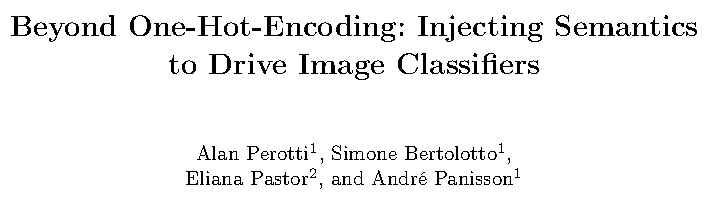
\includegraphics[width=.8\linewidth]{figures/02/paper_title.pdf}
  \end{figure}
  \begin{figure}
    \centering
    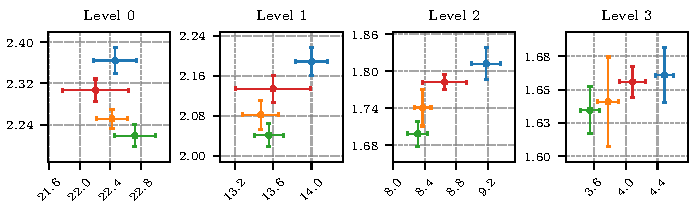
\includegraphics[width=.8\linewidth]{figures/02/paper_errors.pdf}
  \end{figure}
  \begin{figure}
    \centering
    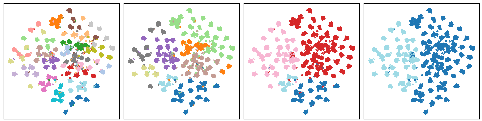
\includegraphics[width=.8\linewidth]{figures/02/paper_features.pdf}
  \end{figure}

  \note{\scriptsize{Questa tecnica per sfruttare le reazioni tra classi usando un
    esplicita gerarchia, è stata già descritta in alcune pubblicazioni.
    Una di queste è un articolo che sarà presentato a xAI 2023.}}
  \note[item]{Abbiamo applicato una simile tecnica per produrre un embedding
    gerarchico e confrontato le performance con quelle ottenute da modelli
    che sfruttano e non la gerachica tra le classi.}
  \note[item]{Per performance intendiamo la quatità di errori, asse orizzontale, e
    la qualità degli errori, asse verticale, a diversi livelli della gerarchica.
    Questi plots saranno ripresi in seguito.}
  \note[item]{Abbiamo inoltre studiato la disposizione spaziale dei features
    vectors, ovvero come sono organizzati nello spazio i vettori del penultimo
    livello del modello associati alle varie immaginni}
  \note[item]{Proiettarli nel piano dà un'indicazione su quali immagini il
    modello pensa siano simili. Ciò che ci attendiamo è la comparsa di cluster
    relativi alle varie classi.}
  \note[item]{Abbiamo usato delle metriche di clustering per quantificare il
    raggruppamento dei features vectors e capire quali modelli producevano una
    rappresentazione interna più strutturata.}
  \note[item]{Un limite di tale approccio è la necessità di avere o poter
    costruire una gerarchica tra le classi. Uno degli approcci presentati supera
    tale limite ricavando gli encoding dai word embeddings delle classi. Ma ciò
    introduce un altri problemi, non tutte le parole hanno un'embedding e una
    parola può avere diversi un significati.}
  \note[item]{Da qui l'idea dei descriptions encodings.}
\end{frame}


  \section{Description Encodings}
  \begin{frame}{Description Encodings}
  Recipe:
  \begin{enumerate}
    \item Use Language Model (e.g. chatGPT) to \alert{generate descriptions}\\
      for each class.
    \item Use Embedding Model (e.g. BERT-like) to \alert{generate embeddings}\\
      for each description.
    \item Use Dimensionality Reduction (e.g. t-SNE) to \alert{generate encodings}\\
      for each embedding.
  \end{enumerate}

    \note[item]{La ricetta per generarli è la seguente.}
  \note[item]{"Uno": usare modelli generativi di testo per produrre
    delle descrizioni delle classi.}
  \note[item]{"Due": usate modelli di embeddings che convertano le descrizioni
    testuali in un vettore di numeri reali detto embeddings. Descrizioni simili
    avranno embeddings simili.}
  \note[item]{"Tre": usare un algoritmo di riduzione della dimensionalità
    mappare gli embeddings in uno spazio di dimensionalità inferiore. Inoltre
    agendo sugli iperparametri di tali algoritmi e possibile modificare la
    distiribuzione spaziale, preservando le relazioni di similarità.}
  \note[item]{Il risulato sono i Description Encodings.}
\end{frame}

\begin{frame}{Description Encodings}
  \begin{itemize}
    \item \texttt{lemon}: \emph{\small``Lemons are \alert{oval-shaped} fruits
      known for their \alert{bright yellow} color and acidic juice.''}
    \item \texttt{pear}: \emph{\small``Pears are fruits a with \alert{rounded
      bottom} and a narrower, \alert{elongated top}.''}
    \item \texttt{apple}: \emph{\small``Apples are \alert{round} fruits that
      come in a variety of colors, including \alert{red}, \alert{green}, and
      \alert{yellow}.''}
  \end{itemize}
  \note[item]{Queste sono esempi di parti di descrizioni di alcune delle
    classi ottenute da un modello generativo.}
  \note[item]{I limoni sono frutti ovali di un giallo brillante, le pere
    hanno la base rotonda e la parte superiore allungata, le mele sono
    tondeggianti rosse, verdi e gialle. Tutte carattiristiche che aiutano a
    distingure visivamente le diverse classi.}
\end{frame}

\begin{frame}{Description Encodings}
  \begin{columns}
    \column{0.65\textwidth}
    \tikzfig{figures/03/embeddings}

    \column{0.35\textwidth}
    \textbf{\textsc{Desideratum}}\\
    \vspace{0.2cm}
    \emph{Distinctive features in the descriptions translate to
    a hierarchy-like structure in the encodings space}
  \end{columns}

  \note[item]{Dalle descrizioni passiamo agli embedding e da questi agli
    encoding. Questa è una rappresentazione 2D semplificata degli encoding.}
  \note[item]{La speranza è che le caratteristiche distintive presenti nelle
    descrizioni si traducano in una struttura gerarchica nello spazio degli
    encoding. Ciò è una conferma che i descriptions encoding riescono a
    ricavare una gerarchia tra le classi dal significato delle descrizioni.}
  \note[item]{Tuttavia gerarchia e similarità tra classi sono concetti
    soggettivi e non necessariamente collegati.}
  \note[item]{Come misura di similarità tra due encodings utilizziamo l'angolo
    tra i due vettori. Mela e pera sono più simili di mela e cane.}
\end{frame}

\begin{frame}{Description Encodings}
  \begin{columns}
    \column{0.65\textwidth}
    \only<1>{\tikzfig{figures/03/encoding_apple_1}}
    \only<2>{\tikzfig{figures/03/encoding_apple_2}}

    \column{0.35\textwidth}
    Align $\psi_\theta$ to $\phi$ with
    \alert{Cosine Distance}.
    \begin{align*}
      \phi &:
      \mathcal{C} \rightarrow \mathbb{R}^{d} \\
      \psi_\theta &:
      \mathcal{X} \rightarrow \mathbb{R}^{d}
    \end{align*}
    \begin{equation*}
      \mathcal{L} := 1 -
      \frac{
        \psi_\theta \cdot \phi
      }{
        \left|\psi_\theta\right|_2
        \left|\phi\right|_2
      }
    \end{equation*}
  \end{columns}

  \note[item]{Consideriamo l'encoding per mela (in blu) e l'output del
    modello non addestrato (arancione).}
  \note[item]{Ora $\phi$ mappa dall'inisieme delle classi a $\mathbb{R}^d$ dove
    la dimensione $d$ e stabilita dall'algoritmo di riduzione di
    dimensionalità. $\mathbb{R}^d$ è anche lo spazio degli output del modello
    che non sono più distribuzioni di probabilità ma semplici vettori con
    componeti reali.}
  \note[item]{Il training consiste nel modificare i parametri $\theta$ in modo
    tale da allineare l'output all'encoding, quindi minimizzare l'angolo compreso.}
  \note[item]{NEXT}
  \note[item]{In questo caso la funzione di loss è la Cosine Distance.}
  \note[item]{La classe predetta dal modello sarà quindi quella associata al
    vettore di encoding più vicino all'output del modello.}
\end{frame}

\begin{frame}{Encondings Comparison}
  \begin{block}{\textsc{One-hot Encoding + Cross Entropy Loss}}
    \begin{itemize}
      \item[\cmark] Battle tested
      \item[\xmark] Ignore classes similarities
    \end{itemize}
  \end{block}
  \begin{block}{\textsc{Hierarchical Encoding + Cross Entropy Loss}}
    \begin{itemize}
      \item[\cmark] Exploit classes similarities
      \item[\xmark] Require a hierarchy
    \end{itemize}
  \end{block}
  \begin{block}{\textsc{Description Encoding + Cosine Distance Loss}}
    \begin{itemize}
      \item[\cmark] Exploit classes similarities
      \item[\cmark] Do not require a hierarchy
    \end{itemize}
  \end{block}

  \note[item]{Riassumendo. One-hot encoding è largamente utilizzato e dà buoni
  risulati. È semplice da implementare e non necessita di informazione extra.
  Tuttavia non tiene conto delle relazioni tra le cassi con la conseguenza che
  scambiare una mela con una pera è equivalente a scambiare una mela con un
  automobile.}
  \note[item]{Hierarchical encoding è una codifica che sfrutta le relazioni tra
  classi basandosi su un'esplicita gerarchia. È quindi applicaile a quei dataset
  per i quali esite o è possibile costruire una gerarchia. Sperimentalmente si
  verifica che è sensibile agli iperparametri conivolti e alla scelta delle
  funzioni che costruiscono le distanze e le probabilità.}
  \note[item]{Infine i modelli che fanno uso di Description Encodings sfruttano
  la relazioni tra classi senza richedere una gerarchica. Costruiscono tali
  relazioni basandosi le conoscenze semantiche apprese dai modelli generativi e
  di embeddings.}
\end{frame}


  \section{Experiments}
  \begin{frame}{Experiments | Datasets}
  \begin{columns}
    \begin{column}{0.35\textwidth}
      \alert{{\large CIFAR-100}}
      \begin{itemize}
        \item 100 classes
        \item 6 hierarchy levels
      \end{itemize}
    \end{column}
    \begin{column}{0.2\textwidth}
      \begin{figure}
        \centering
        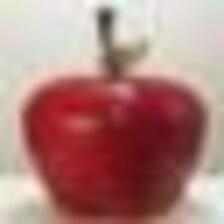
\includegraphics[width=.7\linewidth]{figures/CIFAR100/example_1.jpg}
        \captionsetup{labelformat=empty, justification=centering, font=scriptsize}
        \caption{\emph{Apple}}
      \end{figure}
    \end{column}
    \begin{column}{0.2\textwidth}
      \begin{figure}
        \centering
        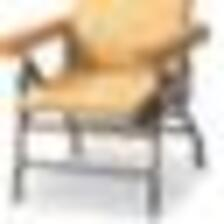
\includegraphics[width=.7\linewidth]{figures/CIFAR100/example_2.jpg}
        \captionsetup{labelformat=empty, justification=centering, font=scriptsize}
        \caption{\emph{Chair}}
      \end{figure}
    \end{column}
    \begin{column}{0.2\textwidth}
      \begin{figure}
        \centering
        
\includegraphics[width=.7\linewidth]{figures/CIFAR100/example_3.jpg}
        \captionsetup{labelformat=empty, justification=centering, font=scriptsize}
        \caption{\emph{Lobster}}
      \end{figure}
    \end{column}
  \end{columns}

  \rule{\linewidth}{0.4pt}

  \begin{columns}
    \begin{column}{0.35\textwidth}
      \alert{{\large iNaturalist19}}
      \begin{itemize}
        \item 1010 classes
        \item 8 hierarchy levels
      \end{itemize}
    \end{column}
    \begin{column}{0.2\textwidth}
      \begin{figure}
        \centering
        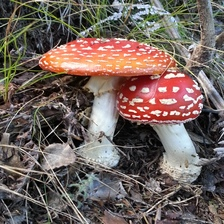
\includegraphics[width=.7\linewidth]{figures/iNaturalist19/example_1.jpg}
        \captionsetup{labelformat=empty, justification=centering, font=scriptsize}
        \caption{\emph{Amanita Muscaria}}
      \end{figure}
    \end{column}
    \begin{column}{0.2\textwidth}
      \begin{figure}
        \centering
        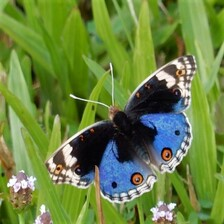
\includegraphics[width=.7\linewidth]{figures/iNaturalist19/example_2.jpg}
        \captionsetup{labelformat=empty, justification=centering, font=scriptsize}
        \caption{\emph{Junonia Orithya}}
      \end{figure}
    \end{column}
    \begin{column}{0.2\textwidth}
      \begin{figure}
        \centering
        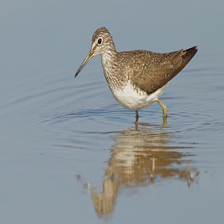
\includegraphics[width=.7\linewidth]{figures/iNaturalist19/example_3.jpg}
        \captionsetup{labelformat=empty, justification=centering, font=scriptsize}
        \caption{\emph{Tringa Ochropus}}
      \end{figure}
    \end{column}
  \end{columns}

  \rule{\linewidth}{0.4pt}

  \begin{columns}
    \begin{column}{0.35\textwidth}
      \alert{{\large tieredImageNet}}
      \begin{itemize}
        \item 608 classes
        \item 13 hierarchy levels
      \end{itemize}
    \end{column}
    \begin{column}{0.2\textwidth}
      \begin{figure}
        \centering
        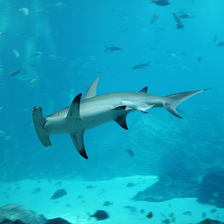
\includegraphics[width=.7\linewidth]{figures/tieredImageNet/example_1.jpg}
        \captionsetup{labelformat=empty, justification=centering, font=scriptsize}
        \caption{\emph{Hammerhead}}
      \end{figure}
    \end{column}
    \begin{column}{0.2\textwidth}
      \begin{figure}
        \centering
        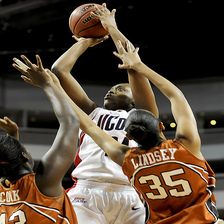
\includegraphics[width=.7\linewidth]{figures/tieredImageNet/example_2.jpg}
        \captionsetup{labelformat=empty, justification=centering, font=scriptsize}
        \caption{\emph{Basketball}}
      \end{figure}
    \end{column}
    \begin{column}{0.2\textwidth}
      \begin{figure}
        \centering
        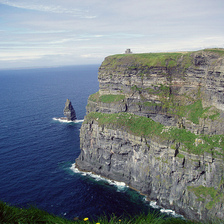
\includegraphics[width=.7\linewidth]{figures/tieredImageNet/example_3.jpg}
        \captionsetup{labelformat=empty, justification=centering, font=scriptsize}
        \caption{\emph{Cliff}}
      \end{figure}
    \end{column}
  \end{columns}

  \note[item]{I datasets utilizzati negli esperimenti sono CIFAR-100,
    iNaturalist19, tieredImageNet.}
  \note[item]{CIFAR-100 è un dataset di immagini a bassa risoluzione, 100
    classi per le quali è definita una gerarchia a 6 livelli. }
  \note[item]{iNaturaluralist sono foto di soggetti nautarali e le etichette
    associate sono il nome scientifico. 1010 classi e gerarchia a 8 livelli}
  \note[item]{tieredImageNet è un sotto insieme di ImageNet, 608 classi e 13
    livelli di gerarchia.}
  \note[item]{Questi dataset muniti di gerarchia sono tra i più utilizzati
    nella classificazione di immagini e danno modo di testare i modelli sotto
    diversi aspetti: diversa risoluzione delle immagini, diversa lingua per i
    nomi delle classi, diversi soggetti, diverso numero di classi.}
\end{frame}


\begin{frame}{Experiments | Metrics}
  Let $\bm{M}$ be the \alert{confusion matrix} \\
  and $\bm{D}$ the \alert{distances matrix} previously introduced.
  \vspace{0.5cm}
  \begin{spreadlines}{15pt}
  \begin{align*}
    \text{Error Rate} &:=
      \frac{\sum \bm{M} - \text{tr} \, \bm{M}}{\sum \bm{M}} \\
    \text{Hierarchical Distance} &:=
      \frac{\sum \bm{M} \odot \bm{D}}{\sum \bm{M}} \\
    \text{Hierarchical Distance Mistake} &:=
      \frac{\sum \bm{M} \odot \bm{D}}{\sum \bm{M} - \text{tr} \, \bm{M}}
  \end{align*}
  \end{spreadlines}

  \note[Item]{Per misurare le performance del modello abbiamo fatto riscorso a
  3 metriche: Error Rate, Hierarchical Distance e Hierarchical Distance Mistake.}
  \note[item]{Queste possono essere definite a partire dalla matrice di
  confusione M e dalla matrice delle distanze D (tipo quella precedentemente
  introdotta).}
  \note[item]{L'Error Rate è il numero di errori commessi diviso il numero di
  esempi nel dataset di Test.}
  \note[item]{Hierarchical Distance la si ottiene moltiplicando M con D elemento
  per elemento, sommando le entrate della matrice risultante e dividendo per il
  totale degli esempi.}
  \note[item]{In Hierarchical distance Mistake nel denominatore è il numero di errori.}
  \note[item]{Error Rate è un indicatore di quanti errori il modello commette,
  mentre Hierarchical Distance Mistake quantifica la gravità di tali errori
  utilizzando come pesi le distanze nella gerarchia.}
\end{frame}


\begin{frame}{Experiments | CIFAR100 --- Performance}
  %% Creator: Matplotlib, PGF backend
%%
%% To include the figure in your LaTeX document, write
%%   \input{<filename>.pgf}
%%
%% Make sure the required packages are loaded in your preamble
%%   \usepackage{pgf}
%%
%% Also ensure that all the required font packages are loaded; for instance,
%% the lmodern package is sometimes necessary when using math font.
%%   \usepackage{lmodern}
%%
%% Figures using additional raster images can only be included by \input if
%% they are in the same directory as the main LaTeX file. For loading figures
%% from other directories you can use the `import` package
%%   \usepackage{import}
%%
%% and then include the figures with
%%   \import{<path to file>}{<filename>.pgf}
%%
%% Matplotlib used the following preamble
%%   
%%   \usepackage{fontspec}
%%   \setmainfont{DejaVuSerif.ttf}[Path=\detokenize{/Users/simo/.local/share/virtualenvs/master-thesis-code/lib/python3.10/site-packages/matplotlib/mpl-data/fonts/ttf/}]
%%   \setsansfont{DejaVuSans.ttf}[Path=\detokenize{/Users/simo/.local/share/virtualenvs/master-thesis-code/lib/python3.10/site-packages/matplotlib/mpl-data/fonts/ttf/}]
%%   \setmonofont{DejaVuSansMono.ttf}[Path=\detokenize{/Users/simo/.local/share/virtualenvs/master-thesis-code/lib/python3.10/site-packages/matplotlib/mpl-data/fonts/ttf/}]
%%   \makeatletter\@ifpackageloaded{underscore}{}{\usepackage[strings]{underscore}}\makeatother
%%
\begingroup%
\makeatletter%
\begin{pgfpicture}%
\pgfpathrectangle{\pgfpointorigin}{\pgfqpoint{4.251970in}{2.627862in}}%
\pgfusepath{use as bounding box, clip}%
\begin{pgfscope}%
\pgfsetbuttcap%
\pgfsetmiterjoin%
\definecolor{currentfill}{rgb}{0.980392,0.980392,0.980392}%
\pgfsetfillcolor{currentfill}%
\pgfsetlinewidth{0.000000pt}%
\definecolor{currentstroke}{rgb}{1.000000,1.000000,1.000000}%
\pgfsetstrokecolor{currentstroke}%
\pgfsetdash{}{0pt}%
\pgfpathmoveto{\pgfqpoint{0.000000in}{0.000000in}}%
\pgfpathlineto{\pgfqpoint{4.251970in}{0.000000in}}%
\pgfpathlineto{\pgfqpoint{4.251970in}{2.627862in}}%
\pgfpathlineto{\pgfqpoint{0.000000in}{2.627862in}}%
\pgfpathlineto{\pgfqpoint{0.000000in}{0.000000in}}%
\pgfpathclose%
\pgfusepath{fill}%
\end{pgfscope}%
\begin{pgfscope}%
\pgfsetbuttcap%
\pgfsetmiterjoin%
\definecolor{currentfill}{rgb}{0.917647,0.917647,0.949020}%
\pgfsetfillcolor{currentfill}%
\pgfsetlinewidth{0.000000pt}%
\definecolor{currentstroke}{rgb}{0.000000,0.000000,0.000000}%
\pgfsetstrokecolor{currentstroke}%
\pgfsetstrokeopacity{0.000000}%
\pgfsetdash{}{0pt}%
\pgfpathmoveto{\pgfqpoint{0.956688in}{0.387285in}}%
\pgfpathlineto{\pgfqpoint{2.790353in}{0.387285in}}%
\pgfpathlineto{\pgfqpoint{2.790353in}{2.390228in}}%
\pgfpathlineto{\pgfqpoint{0.956688in}{2.390228in}}%
\pgfpathlineto{\pgfqpoint{0.956688in}{0.387285in}}%
\pgfpathclose%
\pgfusepath{fill}%
\end{pgfscope}%
\begin{pgfscope}%
\definecolor{textcolor}{rgb}{0.137255,0.215686,0.231373}%
\pgfsetstrokecolor{textcolor}%
\pgfsetfillcolor{textcolor}%
\pgftext[x=1.160428in,y=0.248396in,,top]{\color{textcolor}\sffamily\fontsize{8.000000}{9.600000}\selectfont 27.0}%
\end{pgfscope}%
\begin{pgfscope}%
\definecolor{textcolor}{rgb}{0.137255,0.215686,0.231373}%
\pgfsetstrokecolor{textcolor}%
\pgfsetfillcolor{textcolor}%
\pgftext[x=1.466039in,y=0.248396in,,top]{\color{textcolor}\sffamily\fontsize{8.000000}{9.600000}\selectfont 27.3}%
\end{pgfscope}%
\begin{pgfscope}%
\definecolor{textcolor}{rgb}{0.137255,0.215686,0.231373}%
\pgfsetstrokecolor{textcolor}%
\pgfsetfillcolor{textcolor}%
\pgftext[x=1.771650in,y=0.248396in,,top]{\color{textcolor}\sffamily\fontsize{8.000000}{9.600000}\selectfont 27.6}%
\end{pgfscope}%
\begin{pgfscope}%
\definecolor{textcolor}{rgb}{0.137255,0.215686,0.231373}%
\pgfsetstrokecolor{textcolor}%
\pgfsetfillcolor{textcolor}%
\pgftext[x=2.077261in,y=0.248396in,,top]{\color{textcolor}\sffamily\fontsize{8.000000}{9.600000}\selectfont 27.9}%
\end{pgfscope}%
\begin{pgfscope}%
\definecolor{textcolor}{rgb}{0.137255,0.215686,0.231373}%
\pgfsetstrokecolor{textcolor}%
\pgfsetfillcolor{textcolor}%
\pgftext[x=2.382872in,y=0.248396in,,top]{\color{textcolor}\sffamily\fontsize{8.000000}{9.600000}\selectfont 28.2}%
\end{pgfscope}%
\begin{pgfscope}%
\definecolor{textcolor}{rgb}{0.137255,0.215686,0.231373}%
\pgfsetstrokecolor{textcolor}%
\pgfsetfillcolor{textcolor}%
\pgftext[x=2.790353in,y=0.248396in,,top]{\color{textcolor}\sffamily\fontsize{8.000000}{9.600000}\selectfont Error \%}%
\end{pgfscope}%
\begin{pgfscope}%
\definecolor{textcolor}{rgb}{0.137255,0.215686,0.231373}%
\pgfsetstrokecolor{textcolor}%
\pgfsetfillcolor{textcolor}%
\pgftext[x=0.570403in, y=0.499149in, left, base]{\color{textcolor}\sffamily\fontsize{8.000000}{9.600000}\selectfont 2.26}%
\end{pgfscope}%
\begin{pgfscope}%
\definecolor{textcolor}{rgb}{0.137255,0.215686,0.231373}%
\pgfsetstrokecolor{textcolor}%
\pgfsetfillcolor{textcolor}%
\pgftext[x=0.570403in, y=0.807294in, left, base]{\color{textcolor}\sffamily\fontsize{8.000000}{9.600000}\selectfont 2.30}%
\end{pgfscope}%
\begin{pgfscope}%
\definecolor{textcolor}{rgb}{0.137255,0.215686,0.231373}%
\pgfsetstrokecolor{textcolor}%
\pgfsetfillcolor{textcolor}%
\pgftext[x=0.570403in, y=1.115439in, left, base]{\color{textcolor}\sffamily\fontsize{8.000000}{9.600000}\selectfont 2.34}%
\end{pgfscope}%
\begin{pgfscope}%
\definecolor{textcolor}{rgb}{0.137255,0.215686,0.231373}%
\pgfsetstrokecolor{textcolor}%
\pgfsetfillcolor{textcolor}%
\pgftext[x=0.570403in, y=1.423583in, left, base]{\color{textcolor}\sffamily\fontsize{8.000000}{9.600000}\selectfont 2.38}%
\end{pgfscope}%
\begin{pgfscope}%
\definecolor{textcolor}{rgb}{0.137255,0.215686,0.231373}%
\pgfsetstrokecolor{textcolor}%
\pgfsetfillcolor{textcolor}%
\pgftext[x=0.570403in, y=1.731728in, left, base]{\color{textcolor}\sffamily\fontsize{8.000000}{9.600000}\selectfont 2.42}%
\end{pgfscope}%
\begin{pgfscope}%
\definecolor{textcolor}{rgb}{0.137255,0.215686,0.231373}%
\pgfsetstrokecolor{textcolor}%
\pgfsetfillcolor{textcolor}%
\pgftext[x=0.570403in, y=2.039873in, left, base]{\color{textcolor}\sffamily\fontsize{8.000000}{9.600000}\selectfont 2.46}%
\end{pgfscope}%
\begin{pgfscope}%
\definecolor{textcolor}{rgb}{0.137255,0.215686,0.231373}%
\pgfsetstrokecolor{textcolor}%
\pgfsetfillcolor{textcolor}%
\pgftext[x=0.155581in, y=2.401783in, left, base]{\color{textcolor}\sffamily\fontsize{8.000000}{9.600000}\selectfont Hierarchical}%
\end{pgfscope}%
\begin{pgfscope}%
\definecolor{textcolor}{rgb}{0.137255,0.215686,0.231373}%
\pgfsetstrokecolor{textcolor}%
\pgfsetfillcolor{textcolor}%
\pgftext[x=0.095142in, y=2.277370in, left, base]{\color{textcolor}\sffamily\fontsize{8.000000}{9.600000}\selectfont dist. mistake}%
\end{pgfscope}%
\begin{pgfscope}%
\pgfpathrectangle{\pgfqpoint{0.956688in}{0.387285in}}{\pgfqpoint{1.833666in}{2.002942in}}%
\pgfusepath{clip}%
\pgfsetbuttcap%
\pgfsetroundjoin%
\pgfsetlinewidth{0.752812pt}%
\definecolor{currentstroke}{rgb}{0.298039,0.447059,0.690196}%
\pgfsetstrokecolor{currentstroke}%
\pgfsetdash{}{0pt}%
\pgfpathmoveto{\pgfqpoint{1.807951in}{1.911346in}}%
\pgfpathlineto{\pgfqpoint{2.660332in}{1.911346in}}%
\pgfusepath{stroke}%
\end{pgfscope}%
\begin{pgfscope}%
\pgfpathrectangle{\pgfqpoint{0.956688in}{0.387285in}}{\pgfqpoint{1.833666in}{2.002942in}}%
\pgfusepath{clip}%
\pgfsetbuttcap%
\pgfsetroundjoin%
\pgfsetlinewidth{0.752812pt}%
\definecolor{currentstroke}{rgb}{0.298039,0.447059,0.690196}%
\pgfsetstrokecolor{currentstroke}%
\pgfsetdash{}{0pt}%
\pgfpathmoveto{\pgfqpoint{2.234141in}{1.789100in}}%
\pgfpathlineto{\pgfqpoint{2.234141in}{2.033592in}}%
\pgfusepath{stroke}%
\end{pgfscope}%
\begin{pgfscope}%
\pgfpathrectangle{\pgfqpoint{0.956688in}{0.387285in}}{\pgfqpoint{1.833666in}{2.002942in}}%
\pgfusepath{clip}%
\pgfsetbuttcap%
\pgfsetroundjoin%
\pgfsetlinewidth{0.752812pt}%
\definecolor{currentstroke}{rgb}{0.921569,0.505882,0.105882}%
\pgfsetstrokecolor{currentstroke}%
\pgfsetdash{}{0pt}%
\pgfpathmoveto{\pgfqpoint{1.609789in}{0.685162in}}%
\pgfpathlineto{\pgfqpoint{2.263571in}{0.685162in}}%
\pgfusepath{stroke}%
\end{pgfscope}%
\begin{pgfscope}%
\pgfpathrectangle{\pgfqpoint{0.956688in}{0.387285in}}{\pgfqpoint{1.833666in}{2.002942in}}%
\pgfusepath{clip}%
\pgfsetbuttcap%
\pgfsetroundjoin%
\pgfsetlinewidth{0.752812pt}%
\definecolor{currentstroke}{rgb}{0.921569,0.505882,0.105882}%
\pgfsetstrokecolor{currentstroke}%
\pgfsetdash{}{0pt}%
\pgfpathmoveto{\pgfqpoint{1.936680in}{0.605056in}}%
\pgfpathlineto{\pgfqpoint{1.936680in}{0.765268in}}%
\pgfusepath{stroke}%
\end{pgfscope}%
\begin{pgfscope}%
\pgfpathrectangle{\pgfqpoint{0.956688in}{0.387285in}}{\pgfqpoint{1.833666in}{2.002942in}}%
\pgfusepath{clip}%
\pgfsetbuttcap%
\pgfsetroundjoin%
\pgfsetlinewidth{0.752812pt}%
\definecolor{currentstroke}{rgb}{0.078431,0.690196,0.239216}%
\pgfsetstrokecolor{currentstroke}%
\pgfsetdash{}{0pt}%
\pgfpathmoveto{\pgfqpoint{1.283327in}{1.024880in}}%
\pgfpathlineto{\pgfqpoint{2.084756in}{1.024880in}}%
\pgfusepath{stroke}%
\end{pgfscope}%
\begin{pgfscope}%
\pgfpathrectangle{\pgfqpoint{0.956688in}{0.387285in}}{\pgfqpoint{1.833666in}{2.002942in}}%
\pgfusepath{clip}%
\pgfsetbuttcap%
\pgfsetroundjoin%
\pgfsetlinewidth{0.752812pt}%
\definecolor{currentstroke}{rgb}{0.078431,0.690196,0.239216}%
\pgfsetstrokecolor{currentstroke}%
\pgfsetdash{}{0pt}%
\pgfpathmoveto{\pgfqpoint{1.684042in}{0.841201in}}%
\pgfpathlineto{\pgfqpoint{1.684042in}{1.208559in}}%
\pgfusepath{stroke}%
\end{pgfscope}%
\begin{pgfscope}%
\pgfpathrectangle{\pgfqpoint{0.956688in}{0.387285in}}{\pgfqpoint{1.833666in}{2.002942in}}%
\pgfusepath{clip}%
\pgfsetbuttcap%
\pgfsetroundjoin%
\definecolor{currentfill}{rgb}{0.298039,0.447059,0.690196}%
\pgfsetfillcolor{currentfill}%
\pgfsetlinewidth{0.000000pt}%
\definecolor{currentstroke}{rgb}{0.298039,0.447059,0.690196}%
\pgfsetstrokecolor{currentstroke}%
\pgfsetdash{}{0pt}%
\pgfsys@defobject{currentmarker}{\pgfqpoint{-0.048611in}{-0.048611in}}{\pgfqpoint{0.048611in}{0.048611in}}{%
\pgfpathmoveto{\pgfqpoint{0.000000in}{-0.048611in}}%
\pgfpathcurveto{\pgfqpoint{0.012892in}{-0.048611in}}{\pgfqpoint{0.025257in}{-0.043489in}}{\pgfqpoint{0.034373in}{-0.034373in}}%
\pgfpathcurveto{\pgfqpoint{0.043489in}{-0.025257in}}{\pgfqpoint{0.048611in}{-0.012892in}}{\pgfqpoint{0.048611in}{0.000000in}}%
\pgfpathcurveto{\pgfqpoint{0.048611in}{0.012892in}}{\pgfqpoint{0.043489in}{0.025257in}}{\pgfqpoint{0.034373in}{0.034373in}}%
\pgfpathcurveto{\pgfqpoint{0.025257in}{0.043489in}}{\pgfqpoint{0.012892in}{0.048611in}}{\pgfqpoint{0.000000in}{0.048611in}}%
\pgfpathcurveto{\pgfqpoint{-0.012892in}{0.048611in}}{\pgfqpoint{-0.025257in}{0.043489in}}{\pgfqpoint{-0.034373in}{0.034373in}}%
\pgfpathcurveto{\pgfqpoint{-0.043489in}{0.025257in}}{\pgfqpoint{-0.048611in}{0.012892in}}{\pgfqpoint{-0.048611in}{0.000000in}}%
\pgfpathcurveto{\pgfqpoint{-0.048611in}{-0.012892in}}{\pgfqpoint{-0.043489in}{-0.025257in}}{\pgfqpoint{-0.034373in}{-0.034373in}}%
\pgfpathcurveto{\pgfqpoint{-0.025257in}{-0.043489in}}{\pgfqpoint{-0.012892in}{-0.048611in}}{\pgfqpoint{0.000000in}{-0.048611in}}%
\pgfpathlineto{\pgfqpoint{0.000000in}{-0.048611in}}%
\pgfpathclose%
\pgfusepath{fill}%
}%
\begin{pgfscope}%
\pgfsys@transformshift{2.234141in}{1.911346in}%
\pgfsys@useobject{currentmarker}{}%
\end{pgfscope}%
\end{pgfscope}%
\begin{pgfscope}%
\pgfpathrectangle{\pgfqpoint{0.956688in}{0.387285in}}{\pgfqpoint{1.833666in}{2.002942in}}%
\pgfusepath{clip}%
\pgfsetbuttcap%
\pgfsetroundjoin%
\definecolor{currentfill}{rgb}{0.921569,0.505882,0.105882}%
\pgfsetfillcolor{currentfill}%
\pgfsetlinewidth{0.000000pt}%
\definecolor{currentstroke}{rgb}{0.921569,0.505882,0.105882}%
\pgfsetstrokecolor{currentstroke}%
\pgfsetdash{}{0pt}%
\pgfsys@defobject{currentmarker}{\pgfqpoint{-0.048611in}{-0.048611in}}{\pgfqpoint{0.048611in}{0.048611in}}{%
\pgfpathmoveto{\pgfqpoint{0.000000in}{-0.048611in}}%
\pgfpathcurveto{\pgfqpoint{0.012892in}{-0.048611in}}{\pgfqpoint{0.025257in}{-0.043489in}}{\pgfqpoint{0.034373in}{-0.034373in}}%
\pgfpathcurveto{\pgfqpoint{0.043489in}{-0.025257in}}{\pgfqpoint{0.048611in}{-0.012892in}}{\pgfqpoint{0.048611in}{0.000000in}}%
\pgfpathcurveto{\pgfqpoint{0.048611in}{0.012892in}}{\pgfqpoint{0.043489in}{0.025257in}}{\pgfqpoint{0.034373in}{0.034373in}}%
\pgfpathcurveto{\pgfqpoint{0.025257in}{0.043489in}}{\pgfqpoint{0.012892in}{0.048611in}}{\pgfqpoint{0.000000in}{0.048611in}}%
\pgfpathcurveto{\pgfqpoint{-0.012892in}{0.048611in}}{\pgfqpoint{-0.025257in}{0.043489in}}{\pgfqpoint{-0.034373in}{0.034373in}}%
\pgfpathcurveto{\pgfqpoint{-0.043489in}{0.025257in}}{\pgfqpoint{-0.048611in}{0.012892in}}{\pgfqpoint{-0.048611in}{0.000000in}}%
\pgfpathcurveto{\pgfqpoint{-0.048611in}{-0.012892in}}{\pgfqpoint{-0.043489in}{-0.025257in}}{\pgfqpoint{-0.034373in}{-0.034373in}}%
\pgfpathcurveto{\pgfqpoint{-0.025257in}{-0.043489in}}{\pgfqpoint{-0.012892in}{-0.048611in}}{\pgfqpoint{0.000000in}{-0.048611in}}%
\pgfpathlineto{\pgfqpoint{0.000000in}{-0.048611in}}%
\pgfpathclose%
\pgfusepath{fill}%
}%
\begin{pgfscope}%
\pgfsys@transformshift{1.936680in}{0.685162in}%
\pgfsys@useobject{currentmarker}{}%
\end{pgfscope}%
\end{pgfscope}%
\begin{pgfscope}%
\pgfpathrectangle{\pgfqpoint{0.956688in}{0.387285in}}{\pgfqpoint{1.833666in}{2.002942in}}%
\pgfusepath{clip}%
\pgfsetbuttcap%
\pgfsetroundjoin%
\definecolor{currentfill}{rgb}{0.078431,0.690196,0.239216}%
\pgfsetfillcolor{currentfill}%
\pgfsetlinewidth{0.000000pt}%
\definecolor{currentstroke}{rgb}{0.078431,0.690196,0.239216}%
\pgfsetstrokecolor{currentstroke}%
\pgfsetdash{}{0pt}%
\pgfsys@defobject{currentmarker}{\pgfqpoint{-0.048611in}{-0.048611in}}{\pgfqpoint{0.048611in}{0.048611in}}{%
\pgfpathmoveto{\pgfqpoint{0.000000in}{-0.048611in}}%
\pgfpathcurveto{\pgfqpoint{0.012892in}{-0.048611in}}{\pgfqpoint{0.025257in}{-0.043489in}}{\pgfqpoint{0.034373in}{-0.034373in}}%
\pgfpathcurveto{\pgfqpoint{0.043489in}{-0.025257in}}{\pgfqpoint{0.048611in}{-0.012892in}}{\pgfqpoint{0.048611in}{0.000000in}}%
\pgfpathcurveto{\pgfqpoint{0.048611in}{0.012892in}}{\pgfqpoint{0.043489in}{0.025257in}}{\pgfqpoint{0.034373in}{0.034373in}}%
\pgfpathcurveto{\pgfqpoint{0.025257in}{0.043489in}}{\pgfqpoint{0.012892in}{0.048611in}}{\pgfqpoint{0.000000in}{0.048611in}}%
\pgfpathcurveto{\pgfqpoint{-0.012892in}{0.048611in}}{\pgfqpoint{-0.025257in}{0.043489in}}{\pgfqpoint{-0.034373in}{0.034373in}}%
\pgfpathcurveto{\pgfqpoint{-0.043489in}{0.025257in}}{\pgfqpoint{-0.048611in}{0.012892in}}{\pgfqpoint{-0.048611in}{0.000000in}}%
\pgfpathcurveto{\pgfqpoint{-0.048611in}{-0.012892in}}{\pgfqpoint{-0.043489in}{-0.025257in}}{\pgfqpoint{-0.034373in}{-0.034373in}}%
\pgfpathcurveto{\pgfqpoint{-0.025257in}{-0.043489in}}{\pgfqpoint{-0.012892in}{-0.048611in}}{\pgfqpoint{0.000000in}{-0.048611in}}%
\pgfpathlineto{\pgfqpoint{0.000000in}{-0.048611in}}%
\pgfpathclose%
\pgfusepath{fill}%
}%
\begin{pgfscope}%
\pgfsys@transformshift{1.684042in}{1.024880in}%
\pgfsys@useobject{currentmarker}{}%
\end{pgfscope}%
\end{pgfscope}%
\begin{pgfscope}%
\pgfsetrectcap%
\pgfsetmiterjoin%
\pgfsetlinewidth{1.003750pt}%
\definecolor{currentstroke}{rgb}{0.917647,0.917647,0.949020}%
\pgfsetstrokecolor{currentstroke}%
\pgfsetdash{}{0pt}%
\pgfpathmoveto{\pgfqpoint{0.956688in}{0.387285in}}%
\pgfpathlineto{\pgfqpoint{0.956688in}{2.390228in}}%
\pgfusepath{stroke}%
\end{pgfscope}%
\begin{pgfscope}%
\pgfsetrectcap%
\pgfsetmiterjoin%
\pgfsetlinewidth{1.003750pt}%
\definecolor{currentstroke}{rgb}{0.917647,0.917647,0.949020}%
\pgfsetstrokecolor{currentstroke}%
\pgfsetdash{}{0pt}%
\pgfpathmoveto{\pgfqpoint{2.790353in}{0.387285in}}%
\pgfpathlineto{\pgfqpoint{2.790353in}{2.390228in}}%
\pgfusepath{stroke}%
\end{pgfscope}%
\begin{pgfscope}%
\pgfsetrectcap%
\pgfsetmiterjoin%
\pgfsetlinewidth{1.003750pt}%
\definecolor{currentstroke}{rgb}{0.917647,0.917647,0.949020}%
\pgfsetstrokecolor{currentstroke}%
\pgfsetdash{}{0pt}%
\pgfpathmoveto{\pgfqpoint{0.956688in}{0.387285in}}%
\pgfpathlineto{\pgfqpoint{2.790353in}{0.387285in}}%
\pgfusepath{stroke}%
\end{pgfscope}%
\begin{pgfscope}%
\pgfsetrectcap%
\pgfsetmiterjoin%
\pgfsetlinewidth{1.003750pt}%
\definecolor{currentstroke}{rgb}{0.917647,0.917647,0.949020}%
\pgfsetstrokecolor{currentstroke}%
\pgfsetdash{}{0pt}%
\pgfpathmoveto{\pgfqpoint{0.956688in}{2.390228in}}%
\pgfpathlineto{\pgfqpoint{2.790353in}{2.390228in}}%
\pgfusepath{stroke}%
\end{pgfscope}%
\begin{pgfscope}%
\pgfsetbuttcap%
\pgfsetroundjoin%
\definecolor{currentfill}{rgb}{0.298039,0.447059,0.690196}%
\pgfsetfillcolor{currentfill}%
\pgfsetlinewidth{0.000000pt}%
\definecolor{currentstroke}{rgb}{0.298039,0.447059,0.690196}%
\pgfsetstrokecolor{currentstroke}%
\pgfsetdash{}{0pt}%
\pgfsys@defobject{currentmarker}{\pgfqpoint{-0.048611in}{-0.048611in}}{\pgfqpoint{0.048611in}{0.048611in}}{%
\pgfpathmoveto{\pgfqpoint{0.000000in}{-0.048611in}}%
\pgfpathcurveto{\pgfqpoint{0.012892in}{-0.048611in}}{\pgfqpoint{0.025257in}{-0.043489in}}{\pgfqpoint{0.034373in}{-0.034373in}}%
\pgfpathcurveto{\pgfqpoint{0.043489in}{-0.025257in}}{\pgfqpoint{0.048611in}{-0.012892in}}{\pgfqpoint{0.048611in}{0.000000in}}%
\pgfpathcurveto{\pgfqpoint{0.048611in}{0.012892in}}{\pgfqpoint{0.043489in}{0.025257in}}{\pgfqpoint{0.034373in}{0.034373in}}%
\pgfpathcurveto{\pgfqpoint{0.025257in}{0.043489in}}{\pgfqpoint{0.012892in}{0.048611in}}{\pgfqpoint{0.000000in}{0.048611in}}%
\pgfpathcurveto{\pgfqpoint{-0.012892in}{0.048611in}}{\pgfqpoint{-0.025257in}{0.043489in}}{\pgfqpoint{-0.034373in}{0.034373in}}%
\pgfpathcurveto{\pgfqpoint{-0.043489in}{0.025257in}}{\pgfqpoint{-0.048611in}{0.012892in}}{\pgfqpoint{-0.048611in}{0.000000in}}%
\pgfpathcurveto{\pgfqpoint{-0.048611in}{-0.012892in}}{\pgfqpoint{-0.043489in}{-0.025257in}}{\pgfqpoint{-0.034373in}{-0.034373in}}%
\pgfpathcurveto{\pgfqpoint{-0.025257in}{-0.043489in}}{\pgfqpoint{-0.012892in}{-0.048611in}}{\pgfqpoint{0.000000in}{-0.048611in}}%
\pgfpathlineto{\pgfqpoint{0.000000in}{-0.048611in}}%
\pgfpathclose%
\pgfusepath{fill}%
}%
\begin{pgfscope}%
\pgfsys@transformshift{3.001464in}{1.784047in}%
\pgfsys@useobject{currentmarker}{}%
\end{pgfscope}%
\end{pgfscope}%
\begin{pgfscope}%
\definecolor{textcolor}{rgb}{0.137255,0.215686,0.231373}%
\pgfsetstrokecolor{textcolor}%
\pgfsetfillcolor{textcolor}%
\pgftext[x=3.201464in, y=1.818921in, left, base]{\color{textcolor}\sffamily\fontsize{8.000000}{9.600000}\selectfont One-hot enc.}%
\end{pgfscope}%
\begin{pgfscope}%
\definecolor{textcolor}{rgb}{0.137255,0.215686,0.231373}%
\pgfsetstrokecolor{textcolor}%
\pgfsetfillcolor{textcolor}%
\pgftext[x=3.201464in, y=1.694507in, left, base]{\color{textcolor}\sffamily\fontsize{8.000000}{9.600000}\selectfont Cross Entropy}%
\end{pgfscope}%
\begin{pgfscope}%
\pgfsetbuttcap%
\pgfsetroundjoin%
\definecolor{currentfill}{rgb}{0.921569,0.505882,0.105882}%
\pgfsetfillcolor{currentfill}%
\pgfsetlinewidth{0.000000pt}%
\definecolor{currentstroke}{rgb}{0.921569,0.505882,0.105882}%
\pgfsetstrokecolor{currentstroke}%
\pgfsetdash{}{0pt}%
\pgfsys@defobject{currentmarker}{\pgfqpoint{-0.048611in}{-0.048611in}}{\pgfqpoint{0.048611in}{0.048611in}}{%
\pgfpathmoveto{\pgfqpoint{0.000000in}{-0.048611in}}%
\pgfpathcurveto{\pgfqpoint{0.012892in}{-0.048611in}}{\pgfqpoint{0.025257in}{-0.043489in}}{\pgfqpoint{0.034373in}{-0.034373in}}%
\pgfpathcurveto{\pgfqpoint{0.043489in}{-0.025257in}}{\pgfqpoint{0.048611in}{-0.012892in}}{\pgfqpoint{0.048611in}{0.000000in}}%
\pgfpathcurveto{\pgfqpoint{0.048611in}{0.012892in}}{\pgfqpoint{0.043489in}{0.025257in}}{\pgfqpoint{0.034373in}{0.034373in}}%
\pgfpathcurveto{\pgfqpoint{0.025257in}{0.043489in}}{\pgfqpoint{0.012892in}{0.048611in}}{\pgfqpoint{0.000000in}{0.048611in}}%
\pgfpathcurveto{\pgfqpoint{-0.012892in}{0.048611in}}{\pgfqpoint{-0.025257in}{0.043489in}}{\pgfqpoint{-0.034373in}{0.034373in}}%
\pgfpathcurveto{\pgfqpoint{-0.043489in}{0.025257in}}{\pgfqpoint{-0.048611in}{0.012892in}}{\pgfqpoint{-0.048611in}{0.000000in}}%
\pgfpathcurveto{\pgfqpoint{-0.048611in}{-0.012892in}}{\pgfqpoint{-0.043489in}{-0.025257in}}{\pgfqpoint{-0.034373in}{-0.034373in}}%
\pgfpathcurveto{\pgfqpoint{-0.025257in}{-0.043489in}}{\pgfqpoint{-0.012892in}{-0.048611in}}{\pgfqpoint{0.000000in}{-0.048611in}}%
\pgfpathlineto{\pgfqpoint{0.000000in}{-0.048611in}}%
\pgfpathclose%
\pgfusepath{fill}%
}%
\begin{pgfscope}%
\pgfsys@transformshift{3.001464in}{1.385436in}%
\pgfsys@useobject{currentmarker}{}%
\end{pgfscope}%
\end{pgfscope}%
\begin{pgfscope}%
\definecolor{textcolor}{rgb}{0.137255,0.215686,0.231373}%
\pgfsetstrokecolor{textcolor}%
\pgfsetfillcolor{textcolor}%
\pgftext[x=3.201464in, y=1.420310in, left, base]{\color{textcolor}\sffamily\fontsize{8.000000}{9.600000}\selectfont Hierarchical enc.}%
\end{pgfscope}%
\begin{pgfscope}%
\definecolor{textcolor}{rgb}{0.137255,0.215686,0.231373}%
\pgfsetstrokecolor{textcolor}%
\pgfsetfillcolor{textcolor}%
\pgftext[x=3.201464in, y=1.295896in, left, base]{\color{textcolor}\sffamily\fontsize{8.000000}{9.600000}\selectfont Cross Entropy}%
\end{pgfscope}%
\begin{pgfscope}%
\pgfsetbuttcap%
\pgfsetroundjoin%
\definecolor{currentfill}{rgb}{0.078431,0.690196,0.239216}%
\pgfsetfillcolor{currentfill}%
\pgfsetlinewidth{0.000000pt}%
\definecolor{currentstroke}{rgb}{0.078431,0.690196,0.239216}%
\pgfsetstrokecolor{currentstroke}%
\pgfsetdash{}{0pt}%
\pgfsys@defobject{currentmarker}{\pgfqpoint{-0.048611in}{-0.048611in}}{\pgfqpoint{0.048611in}{0.048611in}}{%
\pgfpathmoveto{\pgfqpoint{0.000000in}{-0.048611in}}%
\pgfpathcurveto{\pgfqpoint{0.012892in}{-0.048611in}}{\pgfqpoint{0.025257in}{-0.043489in}}{\pgfqpoint{0.034373in}{-0.034373in}}%
\pgfpathcurveto{\pgfqpoint{0.043489in}{-0.025257in}}{\pgfqpoint{0.048611in}{-0.012892in}}{\pgfqpoint{0.048611in}{0.000000in}}%
\pgfpathcurveto{\pgfqpoint{0.048611in}{0.012892in}}{\pgfqpoint{0.043489in}{0.025257in}}{\pgfqpoint{0.034373in}{0.034373in}}%
\pgfpathcurveto{\pgfqpoint{0.025257in}{0.043489in}}{\pgfqpoint{0.012892in}{0.048611in}}{\pgfqpoint{0.000000in}{0.048611in}}%
\pgfpathcurveto{\pgfqpoint{-0.012892in}{0.048611in}}{\pgfqpoint{-0.025257in}{0.043489in}}{\pgfqpoint{-0.034373in}{0.034373in}}%
\pgfpathcurveto{\pgfqpoint{-0.043489in}{0.025257in}}{\pgfqpoint{-0.048611in}{0.012892in}}{\pgfqpoint{-0.048611in}{0.000000in}}%
\pgfpathcurveto{\pgfqpoint{-0.048611in}{-0.012892in}}{\pgfqpoint{-0.043489in}{-0.025257in}}{\pgfqpoint{-0.034373in}{-0.034373in}}%
\pgfpathcurveto{\pgfqpoint{-0.025257in}{-0.043489in}}{\pgfqpoint{-0.012892in}{-0.048611in}}{\pgfqpoint{0.000000in}{-0.048611in}}%
\pgfpathlineto{\pgfqpoint{0.000000in}{-0.048611in}}%
\pgfpathclose%
\pgfusepath{fill}%
}%
\begin{pgfscope}%
\pgfsys@transformshift{3.001464in}{0.986825in}%
\pgfsys@useobject{currentmarker}{}%
\end{pgfscope}%
\end{pgfscope}%
\begin{pgfscope}%
\definecolor{textcolor}{rgb}{0.137255,0.215686,0.231373}%
\pgfsetstrokecolor{textcolor}%
\pgfsetfillcolor{textcolor}%
\pgftext[x=3.201464in, y=1.021699in, left, base]{\color{textcolor}\sffamily\fontsize{8.000000}{9.600000}\selectfont Description enc.}%
\end{pgfscope}%
\begin{pgfscope}%
\definecolor{textcolor}{rgb}{0.137255,0.215686,0.231373}%
\pgfsetstrokecolor{textcolor}%
\pgfsetfillcolor{textcolor}%
\pgftext[x=3.201464in, y=0.897285in, left, base]{\color{textcolor}\sffamily\fontsize{8.000000}{9.600000}\selectfont Cosine Distance}%
\end{pgfscope}%
\end{pgfpicture}%
\makeatother%
\endgroup%


  \note[item]{Usando Error rate e Hierarchical Distance Mistake is può
    costruire il seguente scatter plot}
  \note[item]{Più un modello è a destra più errori commette, più è in alto più
    gli errori saranno gravi.}
  \note[item]{Questi sono i risultati ottenuti per CIFAR100 e i modelli che
    sfruttano la gerarchia commettono errori meno gravi.}
\end{frame}

\begin{frame}{Experiments | CIFAR100 --- Description Encodings}
  %% Creator: Matplotlib, PGF backend
%%
%% To include the figure in your LaTeX document, write
%%   \input{<filename>.pgf}
%%
%% Make sure the required packages are loaded in your preamble
%%   \usepackage{pgf}
%%
%% Also ensure that all the required font packages are loaded; for instance,
%% the lmodern package is sometimes necessary when using math font.
%%   \usepackage{lmodern}
%%
%% Figures using additional raster images can only be included by \input if
%% they are in the same directory as the main LaTeX file. For loading figures
%% from other directories you can use the `import` package
%%   \usepackage{import}
%%
%% and then include the figures with
%%   \import{<path to file>}{<filename>.pgf}
%%
%% Matplotlib used the following preamble
%%   
%%   \usepackage{fontspec}
%%   \setmainfont{DejaVuSerif.ttf}[Path=\detokenize{/Users/simo/.local/share/virtualenvs/master-thesis-code/lib/python3.10/site-packages/matplotlib/mpl-data/fonts/ttf/}]
%%   \setsansfont{DejaVuSans.ttf}[Path=\detokenize{/Users/simo/.local/share/virtualenvs/master-thesis-code/lib/python3.10/site-packages/matplotlib/mpl-data/fonts/ttf/}]
%%   \setmonofont{DejaVuSansMono.ttf}[Path=\detokenize{/Users/simo/.local/share/virtualenvs/master-thesis-code/lib/python3.10/site-packages/matplotlib/mpl-data/fonts/ttf/}]
%%   \makeatletter\@ifpackageloaded{underscore}{}{\usepackage[strings]{underscore}}\makeatother
%%
\begingroup%
\makeatletter%
\begin{pgfpicture}%
\pgfpathrectangle{\pgfpointorigin}{\pgfqpoint{4.251970in}{2.627862in}}%
\pgfusepath{use as bounding box, clip}%
\begin{pgfscope}%
\pgfsetbuttcap%
\pgfsetmiterjoin%
\definecolor{currentfill}{rgb}{0.980392,0.980392,0.980392}%
\pgfsetfillcolor{currentfill}%
\pgfsetlinewidth{0.000000pt}%
\definecolor{currentstroke}{rgb}{1.000000,1.000000,1.000000}%
\pgfsetstrokecolor{currentstroke}%
\pgfsetdash{}{0pt}%
\pgfpathmoveto{\pgfqpoint{0.000000in}{0.000000in}}%
\pgfpathlineto{\pgfqpoint{4.251970in}{0.000000in}}%
\pgfpathlineto{\pgfqpoint{4.251970in}{2.627862in}}%
\pgfpathlineto{\pgfqpoint{0.000000in}{2.627862in}}%
\pgfpathlineto{\pgfqpoint{0.000000in}{0.000000in}}%
\pgfpathclose%
\pgfusepath{fill}%
\end{pgfscope}%
\begin{pgfscope}%
\pgfsetbuttcap%
\pgfsetmiterjoin%
\definecolor{currentfill}{rgb}{0.917647,0.917647,0.949020}%
\pgfsetfillcolor{currentfill}%
\pgfsetlinewidth{0.000000pt}%
\definecolor{currentstroke}{rgb}{0.000000,0.000000,0.000000}%
\pgfsetstrokecolor{currentstroke}%
\pgfsetstrokeopacity{0.000000}%
\pgfsetdash{}{0pt}%
\pgfpathmoveto{\pgfqpoint{0.150000in}{0.163259in}}%
\pgfpathlineto{\pgfqpoint{2.423623in}{0.163259in}}%
\pgfpathlineto{\pgfqpoint{2.423623in}{2.464603in}}%
\pgfpathlineto{\pgfqpoint{0.150000in}{2.464603in}}%
\pgfpathlineto{\pgfqpoint{0.150000in}{0.163259in}}%
\pgfpathclose%
\pgfusepath{fill}%
\end{pgfscope}%
\begin{pgfscope}%
\pgfpathrectangle{\pgfqpoint{0.150000in}{0.163259in}}{\pgfqpoint{2.273623in}{2.301344in}}%
\pgfusepath{clip}%
\pgfsetbuttcap%
\pgfsetroundjoin%
\definecolor{currentfill}{rgb}{0.200000,0.133333,0.533333}%
\pgfsetfillcolor{currentfill}%
\pgfsetlinewidth{0.301125pt}%
\definecolor{currentstroke}{rgb}{0.200000,0.133333,0.533333}%
\pgfsetstrokecolor{currentstroke}%
\pgfsetdash{}{0pt}%
\pgfpathmoveto{\pgfqpoint{1.570181in}{0.638042in}}%
\pgfpathcurveto{\pgfqpoint{1.578418in}{0.638042in}}{\pgfqpoint{1.586318in}{0.641314in}}{\pgfqpoint{1.592142in}{0.647138in}}%
\pgfpathcurveto{\pgfqpoint{1.597966in}{0.652962in}}{\pgfqpoint{1.601238in}{0.660862in}}{\pgfqpoint{1.601238in}{0.669098in}}%
\pgfpathcurveto{\pgfqpoint{1.601238in}{0.677335in}}{\pgfqpoint{1.597966in}{0.685235in}}{\pgfqpoint{1.592142in}{0.691059in}}%
\pgfpathcurveto{\pgfqpoint{1.586318in}{0.696883in}}{\pgfqpoint{1.578418in}{0.700155in}}{\pgfqpoint{1.570181in}{0.700155in}}%
\pgfpathcurveto{\pgfqpoint{1.561945in}{0.700155in}}{\pgfqpoint{1.554045in}{0.696883in}}{\pgfqpoint{1.548221in}{0.691059in}}%
\pgfpathcurveto{\pgfqpoint{1.542397in}{0.685235in}}{\pgfqpoint{1.539125in}{0.677335in}}{\pgfqpoint{1.539125in}{0.669098in}}%
\pgfpathcurveto{\pgfqpoint{1.539125in}{0.660862in}}{\pgfqpoint{1.542397in}{0.652962in}}{\pgfqpoint{1.548221in}{0.647138in}}%
\pgfpathcurveto{\pgfqpoint{1.554045in}{0.641314in}}{\pgfqpoint{1.561945in}{0.638042in}}{\pgfqpoint{1.570181in}{0.638042in}}%
\pgfpathlineto{\pgfqpoint{1.570181in}{0.638042in}}%
\pgfpathclose%
\pgfusepath{stroke,fill}%
\end{pgfscope}%
\begin{pgfscope}%
\pgfpathrectangle{\pgfqpoint{0.150000in}{0.163259in}}{\pgfqpoint{2.273623in}{2.301344in}}%
\pgfusepath{clip}%
\pgfsetbuttcap%
\pgfsetroundjoin%
\definecolor{currentfill}{rgb}{0.400000,0.600000,0.800000}%
\pgfsetfillcolor{currentfill}%
\pgfsetlinewidth{0.301125pt}%
\definecolor{currentstroke}{rgb}{0.400000,0.600000,0.800000}%
\pgfsetstrokecolor{currentstroke}%
\pgfsetdash{}{0pt}%
\pgfpathmoveto{\pgfqpoint{0.253773in}{1.503012in}}%
\pgfpathcurveto{\pgfqpoint{0.262010in}{1.503012in}}{\pgfqpoint{0.269910in}{1.506285in}}{\pgfqpoint{0.275734in}{1.512108in}}%
\pgfpathcurveto{\pgfqpoint{0.281558in}{1.517932in}}{\pgfqpoint{0.284830in}{1.525832in}}{\pgfqpoint{0.284830in}{1.534069in}}%
\pgfpathcurveto{\pgfqpoint{0.284830in}{1.542305in}}{\pgfqpoint{0.281558in}{1.550205in}}{\pgfqpoint{0.275734in}{1.556029in}}%
\pgfpathcurveto{\pgfqpoint{0.269910in}{1.561853in}}{\pgfqpoint{0.262010in}{1.565125in}}{\pgfqpoint{0.253773in}{1.565125in}}%
\pgfpathcurveto{\pgfqpoint{0.245537in}{1.565125in}}{\pgfqpoint{0.237637in}{1.561853in}}{\pgfqpoint{0.231813in}{1.556029in}}%
\pgfpathcurveto{\pgfqpoint{0.225989in}{1.550205in}}{\pgfqpoint{0.222717in}{1.542305in}}{\pgfqpoint{0.222717in}{1.534069in}}%
\pgfpathcurveto{\pgfqpoint{0.222717in}{1.525832in}}{\pgfqpoint{0.225989in}{1.517932in}}{\pgfqpoint{0.231813in}{1.512108in}}%
\pgfpathcurveto{\pgfqpoint{0.237637in}{1.506285in}}{\pgfqpoint{0.245537in}{1.503012in}}{\pgfqpoint{0.253773in}{1.503012in}}%
\pgfpathlineto{\pgfqpoint{0.253773in}{1.503012in}}%
\pgfpathclose%
\pgfusepath{stroke,fill}%
\end{pgfscope}%
\begin{pgfscope}%
\pgfpathrectangle{\pgfqpoint{0.150000in}{0.163259in}}{\pgfqpoint{2.273623in}{2.301344in}}%
\pgfusepath{clip}%
\pgfsetbuttcap%
\pgfsetroundjoin%
\definecolor{currentfill}{rgb}{0.533333,0.800000,0.933333}%
\pgfsetfillcolor{currentfill}%
\pgfsetlinewidth{0.301125pt}%
\definecolor{currentstroke}{rgb}{0.533333,0.800000,0.933333}%
\pgfsetstrokecolor{currentstroke}%
\pgfsetdash{}{0pt}%
\pgfpathmoveto{\pgfqpoint{1.578441in}{2.273265in}}%
\pgfpathcurveto{\pgfqpoint{1.586678in}{2.273265in}}{\pgfqpoint{1.594578in}{2.276537in}}{\pgfqpoint{1.600402in}{2.282361in}}%
\pgfpathcurveto{\pgfqpoint{1.606225in}{2.288185in}}{\pgfqpoint{1.609498in}{2.296085in}}{\pgfqpoint{1.609498in}{2.304321in}}%
\pgfpathcurveto{\pgfqpoint{1.609498in}{2.312557in}}{\pgfqpoint{1.606225in}{2.320457in}}{\pgfqpoint{1.600402in}{2.326281in}}%
\pgfpathcurveto{\pgfqpoint{1.594578in}{2.332105in}}{\pgfqpoint{1.586678in}{2.335378in}}{\pgfqpoint{1.578441in}{2.335378in}}%
\pgfpathcurveto{\pgfqpoint{1.570205in}{2.335378in}}{\pgfqpoint{1.562305in}{2.332105in}}{\pgfqpoint{1.556481in}{2.326281in}}%
\pgfpathcurveto{\pgfqpoint{1.550657in}{2.320457in}}{\pgfqpoint{1.547385in}{2.312557in}}{\pgfqpoint{1.547385in}{2.304321in}}%
\pgfpathcurveto{\pgfqpoint{1.547385in}{2.296085in}}{\pgfqpoint{1.550657in}{2.288185in}}{\pgfqpoint{1.556481in}{2.282361in}}%
\pgfpathcurveto{\pgfqpoint{1.562305in}{2.276537in}}{\pgfqpoint{1.570205in}{2.273265in}}{\pgfqpoint{1.578441in}{2.273265in}}%
\pgfpathlineto{\pgfqpoint{1.578441in}{2.273265in}}%
\pgfpathclose%
\pgfusepath{stroke,fill}%
\end{pgfscope}%
\begin{pgfscope}%
\pgfpathrectangle{\pgfqpoint{0.150000in}{0.163259in}}{\pgfqpoint{2.273623in}{2.301344in}}%
\pgfusepath{clip}%
\pgfsetbuttcap%
\pgfsetroundjoin%
\definecolor{currentfill}{rgb}{0.533333,0.800000,0.933333}%
\pgfsetfillcolor{currentfill}%
\pgfsetlinewidth{0.301125pt}%
\definecolor{currentstroke}{rgb}{0.533333,0.800000,0.933333}%
\pgfsetstrokecolor{currentstroke}%
\pgfsetdash{}{0pt}%
\pgfpathmoveto{\pgfqpoint{0.752267in}{1.854931in}}%
\pgfpathcurveto{\pgfqpoint{0.760504in}{1.854931in}}{\pgfqpoint{0.768404in}{1.858203in}}{\pgfqpoint{0.774228in}{1.864027in}}%
\pgfpathcurveto{\pgfqpoint{0.780052in}{1.869851in}}{\pgfqpoint{0.783324in}{1.877751in}}{\pgfqpoint{0.783324in}{1.885987in}}%
\pgfpathcurveto{\pgfqpoint{0.783324in}{1.894223in}}{\pgfqpoint{0.780052in}{1.902123in}}{\pgfqpoint{0.774228in}{1.907947in}}%
\pgfpathcurveto{\pgfqpoint{0.768404in}{1.913771in}}{\pgfqpoint{0.760504in}{1.917044in}}{\pgfqpoint{0.752267in}{1.917044in}}%
\pgfpathcurveto{\pgfqpoint{0.744031in}{1.917044in}}{\pgfqpoint{0.736131in}{1.913771in}}{\pgfqpoint{0.730307in}{1.907947in}}%
\pgfpathcurveto{\pgfqpoint{0.724483in}{1.902123in}}{\pgfqpoint{0.721211in}{1.894223in}}{\pgfqpoint{0.721211in}{1.885987in}}%
\pgfpathcurveto{\pgfqpoint{0.721211in}{1.877751in}}{\pgfqpoint{0.724483in}{1.869851in}}{\pgfqpoint{0.730307in}{1.864027in}}%
\pgfpathcurveto{\pgfqpoint{0.736131in}{1.858203in}}{\pgfqpoint{0.744031in}{1.854931in}}{\pgfqpoint{0.752267in}{1.854931in}}%
\pgfpathlineto{\pgfqpoint{0.752267in}{1.854931in}}%
\pgfpathclose%
\pgfusepath{stroke,fill}%
\end{pgfscope}%
\begin{pgfscope}%
\pgfpathrectangle{\pgfqpoint{0.150000in}{0.163259in}}{\pgfqpoint{2.273623in}{2.301344in}}%
\pgfusepath{clip}%
\pgfsetbuttcap%
\pgfsetroundjoin%
\definecolor{currentfill}{rgb}{0.400000,0.600000,0.800000}%
\pgfsetfillcolor{currentfill}%
\pgfsetlinewidth{0.301125pt}%
\definecolor{currentstroke}{rgb}{0.400000,0.600000,0.800000}%
\pgfsetstrokecolor{currentstroke}%
\pgfsetdash{}{0pt}%
\pgfpathmoveto{\pgfqpoint{0.693475in}{1.683400in}}%
\pgfpathcurveto{\pgfqpoint{0.701711in}{1.683400in}}{\pgfqpoint{0.709611in}{1.686673in}}{\pgfqpoint{0.715435in}{1.692497in}}%
\pgfpathcurveto{\pgfqpoint{0.721259in}{1.698321in}}{\pgfqpoint{0.724531in}{1.706221in}}{\pgfqpoint{0.724531in}{1.714457in}}%
\pgfpathcurveto{\pgfqpoint{0.724531in}{1.722693in}}{\pgfqpoint{0.721259in}{1.730593in}}{\pgfqpoint{0.715435in}{1.736417in}}%
\pgfpathcurveto{\pgfqpoint{0.709611in}{1.742241in}}{\pgfqpoint{0.701711in}{1.745513in}}{\pgfqpoint{0.693475in}{1.745513in}}%
\pgfpathcurveto{\pgfqpoint{0.685239in}{1.745513in}}{\pgfqpoint{0.677339in}{1.742241in}}{\pgfqpoint{0.671515in}{1.736417in}}%
\pgfpathcurveto{\pgfqpoint{0.665691in}{1.730593in}}{\pgfqpoint{0.662418in}{1.722693in}}{\pgfqpoint{0.662418in}{1.714457in}}%
\pgfpathcurveto{\pgfqpoint{0.662418in}{1.706221in}}{\pgfqpoint{0.665691in}{1.698321in}}{\pgfqpoint{0.671515in}{1.692497in}}%
\pgfpathcurveto{\pgfqpoint{0.677339in}{1.686673in}}{\pgfqpoint{0.685239in}{1.683400in}}{\pgfqpoint{0.693475in}{1.683400in}}%
\pgfpathlineto{\pgfqpoint{0.693475in}{1.683400in}}%
\pgfpathclose%
\pgfusepath{stroke,fill}%
\end{pgfscope}%
\begin{pgfscope}%
\pgfpathrectangle{\pgfqpoint{0.150000in}{0.163259in}}{\pgfqpoint{2.273623in}{2.301344in}}%
\pgfusepath{clip}%
\pgfsetbuttcap%
\pgfsetroundjoin%
\definecolor{currentfill}{rgb}{0.066667,0.466667,0.200000}%
\pgfsetfillcolor{currentfill}%
\pgfsetlinewidth{0.301125pt}%
\definecolor{currentstroke}{rgb}{0.066667,0.466667,0.200000}%
\pgfsetstrokecolor{currentstroke}%
\pgfsetdash{}{0pt}%
\pgfpathmoveto{\pgfqpoint{2.058853in}{1.165754in}}%
\pgfpathcurveto{\pgfqpoint{2.067089in}{1.165754in}}{\pgfqpoint{2.074989in}{1.169026in}}{\pgfqpoint{2.080813in}{1.174850in}}%
\pgfpathcurveto{\pgfqpoint{2.086637in}{1.180674in}}{\pgfqpoint{2.089909in}{1.188574in}}{\pgfqpoint{2.089909in}{1.196810in}}%
\pgfpathcurveto{\pgfqpoint{2.089909in}{1.205047in}}{\pgfqpoint{2.086637in}{1.212947in}}{\pgfqpoint{2.080813in}{1.218771in}}%
\pgfpathcurveto{\pgfqpoint{2.074989in}{1.224594in}}{\pgfqpoint{2.067089in}{1.227867in}}{\pgfqpoint{2.058853in}{1.227867in}}%
\pgfpathcurveto{\pgfqpoint{2.050616in}{1.227867in}}{\pgfqpoint{2.042716in}{1.224594in}}{\pgfqpoint{2.036892in}{1.218771in}}%
\pgfpathcurveto{\pgfqpoint{2.031068in}{1.212947in}}{\pgfqpoint{2.027796in}{1.205047in}}{\pgfqpoint{2.027796in}{1.196810in}}%
\pgfpathcurveto{\pgfqpoint{2.027796in}{1.188574in}}{\pgfqpoint{2.031068in}{1.180674in}}{\pgfqpoint{2.036892in}{1.174850in}}%
\pgfpathcurveto{\pgfqpoint{2.042716in}{1.169026in}}{\pgfqpoint{2.050616in}{1.165754in}}{\pgfqpoint{2.058853in}{1.165754in}}%
\pgfpathlineto{\pgfqpoint{2.058853in}{1.165754in}}%
\pgfpathclose%
\pgfusepath{stroke,fill}%
\end{pgfscope}%
\begin{pgfscope}%
\pgfpathrectangle{\pgfqpoint{0.150000in}{0.163259in}}{\pgfqpoint{2.273623in}{2.301344in}}%
\pgfusepath{clip}%
\pgfsetbuttcap%
\pgfsetroundjoin%
\definecolor{currentfill}{rgb}{0.600000,0.600000,0.200000}%
\pgfsetfillcolor{currentfill}%
\pgfsetlinewidth{0.301125pt}%
\definecolor{currentstroke}{rgb}{0.600000,0.600000,0.200000}%
\pgfsetstrokecolor{currentstroke}%
\pgfsetdash{}{0pt}%
\pgfpathmoveto{\pgfqpoint{0.987960in}{0.674615in}}%
\pgfpathcurveto{\pgfqpoint{0.996196in}{0.674615in}}{\pgfqpoint{1.004096in}{0.677887in}}{\pgfqpoint{1.009920in}{0.683711in}}%
\pgfpathcurveto{\pgfqpoint{1.015744in}{0.689535in}}{\pgfqpoint{1.019017in}{0.697435in}}{\pgfqpoint{1.019017in}{0.705672in}}%
\pgfpathcurveto{\pgfqpoint{1.019017in}{0.713908in}}{\pgfqpoint{1.015744in}{0.721808in}}{\pgfqpoint{1.009920in}{0.727632in}}%
\pgfpathcurveto{\pgfqpoint{1.004096in}{0.733456in}}{\pgfqpoint{0.996196in}{0.736728in}}{\pgfqpoint{0.987960in}{0.736728in}}%
\pgfpathcurveto{\pgfqpoint{0.979724in}{0.736728in}}{\pgfqpoint{0.971824in}{0.733456in}}{\pgfqpoint{0.966000in}{0.727632in}}%
\pgfpathcurveto{\pgfqpoint{0.960176in}{0.721808in}}{\pgfqpoint{0.956904in}{0.713908in}}{\pgfqpoint{0.956904in}{0.705672in}}%
\pgfpathcurveto{\pgfqpoint{0.956904in}{0.697435in}}{\pgfqpoint{0.960176in}{0.689535in}}{\pgfqpoint{0.966000in}{0.683711in}}%
\pgfpathcurveto{\pgfqpoint{0.971824in}{0.677887in}}{\pgfqpoint{0.979724in}{0.674615in}}{\pgfqpoint{0.987960in}{0.674615in}}%
\pgfpathlineto{\pgfqpoint{0.987960in}{0.674615in}}%
\pgfpathclose%
\pgfusepath{stroke,fill}%
\end{pgfscope}%
\begin{pgfscope}%
\pgfpathrectangle{\pgfqpoint{0.150000in}{0.163259in}}{\pgfqpoint{2.273623in}{2.301344in}}%
\pgfusepath{clip}%
\pgfsetbuttcap%
\pgfsetroundjoin%
\definecolor{currentfill}{rgb}{0.600000,0.600000,0.200000}%
\pgfsetfillcolor{currentfill}%
\pgfsetlinewidth{0.301125pt}%
\definecolor{currentstroke}{rgb}{0.600000,0.600000,0.200000}%
\pgfsetstrokecolor{currentstroke}%
\pgfsetdash{}{0pt}%
\pgfpathmoveto{\pgfqpoint{0.924877in}{0.743385in}}%
\pgfpathcurveto{\pgfqpoint{0.933113in}{0.743385in}}{\pgfqpoint{0.941013in}{0.746657in}}{\pgfqpoint{0.946837in}{0.752481in}}%
\pgfpathcurveto{\pgfqpoint{0.952661in}{0.758305in}}{\pgfqpoint{0.955933in}{0.766205in}}{\pgfqpoint{0.955933in}{0.774441in}}%
\pgfpathcurveto{\pgfqpoint{0.955933in}{0.782678in}}{\pgfqpoint{0.952661in}{0.790578in}}{\pgfqpoint{0.946837in}{0.796402in}}%
\pgfpathcurveto{\pgfqpoint{0.941013in}{0.802226in}}{\pgfqpoint{0.933113in}{0.805498in}}{\pgfqpoint{0.924877in}{0.805498in}}%
\pgfpathcurveto{\pgfqpoint{0.916641in}{0.805498in}}{\pgfqpoint{0.908741in}{0.802226in}}{\pgfqpoint{0.902917in}{0.796402in}}%
\pgfpathcurveto{\pgfqpoint{0.897093in}{0.790578in}}{\pgfqpoint{0.893820in}{0.782678in}}{\pgfqpoint{0.893820in}{0.774441in}}%
\pgfpathcurveto{\pgfqpoint{0.893820in}{0.766205in}}{\pgfqpoint{0.897093in}{0.758305in}}{\pgfqpoint{0.902917in}{0.752481in}}%
\pgfpathcurveto{\pgfqpoint{0.908741in}{0.746657in}}{\pgfqpoint{0.916641in}{0.743385in}}{\pgfqpoint{0.924877in}{0.743385in}}%
\pgfpathlineto{\pgfqpoint{0.924877in}{0.743385in}}%
\pgfpathclose%
\pgfusepath{stroke,fill}%
\end{pgfscope}%
\begin{pgfscope}%
\pgfpathrectangle{\pgfqpoint{0.150000in}{0.163259in}}{\pgfqpoint{2.273623in}{2.301344in}}%
\pgfusepath{clip}%
\pgfsetbuttcap%
\pgfsetroundjoin%
\definecolor{currentfill}{rgb}{0.866667,0.800000,0.466667}%
\pgfsetfillcolor{currentfill}%
\pgfsetlinewidth{0.301125pt}%
\definecolor{currentstroke}{rgb}{0.866667,0.800000,0.466667}%
\pgfsetstrokecolor{currentstroke}%
\pgfsetdash{}{0pt}%
\pgfpathmoveto{\pgfqpoint{2.133120in}{2.058554in}}%
\pgfpathcurveto{\pgfqpoint{2.141356in}{2.058554in}}{\pgfqpoint{2.149256in}{2.061826in}}{\pgfqpoint{2.155080in}{2.067650in}}%
\pgfpathcurveto{\pgfqpoint{2.160904in}{2.073474in}}{\pgfqpoint{2.164176in}{2.081374in}}{\pgfqpoint{2.164176in}{2.089611in}}%
\pgfpathcurveto{\pgfqpoint{2.164176in}{2.097847in}}{\pgfqpoint{2.160904in}{2.105747in}}{\pgfqpoint{2.155080in}{2.111571in}}%
\pgfpathcurveto{\pgfqpoint{2.149256in}{2.117395in}}{\pgfqpoint{2.141356in}{2.120667in}}{\pgfqpoint{2.133120in}{2.120667in}}%
\pgfpathcurveto{\pgfqpoint{2.124884in}{2.120667in}}{\pgfqpoint{2.116984in}{2.117395in}}{\pgfqpoint{2.111160in}{2.111571in}}%
\pgfpathcurveto{\pgfqpoint{2.105336in}{2.105747in}}{\pgfqpoint{2.102063in}{2.097847in}}{\pgfqpoint{2.102063in}{2.089611in}}%
\pgfpathcurveto{\pgfqpoint{2.102063in}{2.081374in}}{\pgfqpoint{2.105336in}{2.073474in}}{\pgfqpoint{2.111160in}{2.067650in}}%
\pgfpathcurveto{\pgfqpoint{2.116984in}{2.061826in}}{\pgfqpoint{2.124884in}{2.058554in}}{\pgfqpoint{2.133120in}{2.058554in}}%
\pgfpathlineto{\pgfqpoint{2.133120in}{2.058554in}}%
\pgfpathclose%
\pgfusepath{stroke,fill}%
\end{pgfscope}%
\begin{pgfscope}%
\pgfpathrectangle{\pgfqpoint{0.150000in}{0.163259in}}{\pgfqpoint{2.273623in}{2.301344in}}%
\pgfusepath{clip}%
\pgfsetbuttcap%
\pgfsetroundjoin%
\definecolor{currentfill}{rgb}{0.066667,0.466667,0.200000}%
\pgfsetfillcolor{currentfill}%
\pgfsetlinewidth{0.301125pt}%
\definecolor{currentstroke}{rgb}{0.066667,0.466667,0.200000}%
\pgfsetstrokecolor{currentstroke}%
\pgfsetdash{}{0pt}%
\pgfpathmoveto{\pgfqpoint{2.320276in}{0.803923in}}%
\pgfpathcurveto{\pgfqpoint{2.328513in}{0.803923in}}{\pgfqpoint{2.336413in}{0.807196in}}{\pgfqpoint{2.342237in}{0.813020in}}%
\pgfpathcurveto{\pgfqpoint{2.348061in}{0.818843in}}{\pgfqpoint{2.351333in}{0.826744in}}{\pgfqpoint{2.351333in}{0.834980in}}%
\pgfpathcurveto{\pgfqpoint{2.351333in}{0.843216in}}{\pgfqpoint{2.348061in}{0.851116in}}{\pgfqpoint{2.342237in}{0.856940in}}%
\pgfpathcurveto{\pgfqpoint{2.336413in}{0.862764in}}{\pgfqpoint{2.328513in}{0.866036in}}{\pgfqpoint{2.320276in}{0.866036in}}%
\pgfpathcurveto{\pgfqpoint{2.312040in}{0.866036in}}{\pgfqpoint{2.304140in}{0.862764in}}{\pgfqpoint{2.298316in}{0.856940in}}%
\pgfpathcurveto{\pgfqpoint{2.292492in}{0.851116in}}{\pgfqpoint{2.289220in}{0.843216in}}{\pgfqpoint{2.289220in}{0.834980in}}%
\pgfpathcurveto{\pgfqpoint{2.289220in}{0.826744in}}{\pgfqpoint{2.292492in}{0.818843in}}{\pgfqpoint{2.298316in}{0.813020in}}%
\pgfpathcurveto{\pgfqpoint{2.304140in}{0.807196in}}{\pgfqpoint{2.312040in}{0.803923in}}{\pgfqpoint{2.320276in}{0.803923in}}%
\pgfpathlineto{\pgfqpoint{2.320276in}{0.803923in}}%
\pgfpathclose%
\pgfusepath{stroke,fill}%
\end{pgfscope}%
\begin{pgfscope}%
\pgfpathrectangle{\pgfqpoint{0.150000in}{0.163259in}}{\pgfqpoint{2.273623in}{2.301344in}}%
\pgfusepath{clip}%
\pgfsetbuttcap%
\pgfsetroundjoin%
\definecolor{currentfill}{rgb}{0.066667,0.466667,0.200000}%
\pgfsetfillcolor{currentfill}%
\pgfsetlinewidth{0.301125pt}%
\definecolor{currentstroke}{rgb}{0.066667,0.466667,0.200000}%
\pgfsetstrokecolor{currentstroke}%
\pgfsetdash{}{0pt}%
\pgfpathmoveto{\pgfqpoint{2.193779in}{0.811541in}}%
\pgfpathcurveto{\pgfqpoint{2.202015in}{0.811541in}}{\pgfqpoint{2.209915in}{0.814814in}}{\pgfqpoint{2.215739in}{0.820638in}}%
\pgfpathcurveto{\pgfqpoint{2.221563in}{0.826461in}}{\pgfqpoint{2.224835in}{0.834362in}}{\pgfqpoint{2.224835in}{0.842598in}}%
\pgfpathcurveto{\pgfqpoint{2.224835in}{0.850834in}}{\pgfqpoint{2.221563in}{0.858734in}}{\pgfqpoint{2.215739in}{0.864558in}}%
\pgfpathcurveto{\pgfqpoint{2.209915in}{0.870382in}}{\pgfqpoint{2.202015in}{0.873654in}}{\pgfqpoint{2.193779in}{0.873654in}}%
\pgfpathcurveto{\pgfqpoint{2.185543in}{0.873654in}}{\pgfqpoint{2.177643in}{0.870382in}}{\pgfqpoint{2.171819in}{0.864558in}}%
\pgfpathcurveto{\pgfqpoint{2.165995in}{0.858734in}}{\pgfqpoint{2.162722in}{0.850834in}}{\pgfqpoint{2.162722in}{0.842598in}}%
\pgfpathcurveto{\pgfqpoint{2.162722in}{0.834362in}}{\pgfqpoint{2.165995in}{0.826461in}}{\pgfqpoint{2.171819in}{0.820638in}}%
\pgfpathcurveto{\pgfqpoint{2.177643in}{0.814814in}}{\pgfqpoint{2.185543in}{0.811541in}}{\pgfqpoint{2.193779in}{0.811541in}}%
\pgfpathlineto{\pgfqpoint{2.193779in}{0.811541in}}%
\pgfpathclose%
\pgfusepath{stroke,fill}%
\end{pgfscope}%
\begin{pgfscope}%
\pgfpathrectangle{\pgfqpoint{0.150000in}{0.163259in}}{\pgfqpoint{2.273623in}{2.301344in}}%
\pgfusepath{clip}%
\pgfsetbuttcap%
\pgfsetroundjoin%
\definecolor{currentfill}{rgb}{0.533333,0.800000,0.933333}%
\pgfsetfillcolor{currentfill}%
\pgfsetlinewidth{0.301125pt}%
\definecolor{currentstroke}{rgb}{0.533333,0.800000,0.933333}%
\pgfsetstrokecolor{currentstroke}%
\pgfsetdash{}{0pt}%
\pgfpathmoveto{\pgfqpoint{1.548403in}{2.199532in}}%
\pgfpathcurveto{\pgfqpoint{1.556640in}{2.199532in}}{\pgfqpoint{1.564540in}{2.202804in}}{\pgfqpoint{1.570364in}{2.208628in}}%
\pgfpathcurveto{\pgfqpoint{1.576187in}{2.214452in}}{\pgfqpoint{1.579460in}{2.222352in}}{\pgfqpoint{1.579460in}{2.230588in}}%
\pgfpathcurveto{\pgfqpoint{1.579460in}{2.238825in}}{\pgfqpoint{1.576187in}{2.246725in}}{\pgfqpoint{1.570364in}{2.252549in}}%
\pgfpathcurveto{\pgfqpoint{1.564540in}{2.258373in}}{\pgfqpoint{1.556640in}{2.261645in}}{\pgfqpoint{1.548403in}{2.261645in}}%
\pgfpathcurveto{\pgfqpoint{1.540167in}{2.261645in}}{\pgfqpoint{1.532267in}{2.258373in}}{\pgfqpoint{1.526443in}{2.252549in}}%
\pgfpathcurveto{\pgfqpoint{1.520619in}{2.246725in}}{\pgfqpoint{1.517347in}{2.238825in}}{\pgfqpoint{1.517347in}{2.230588in}}%
\pgfpathcurveto{\pgfqpoint{1.517347in}{2.222352in}}{\pgfqpoint{1.520619in}{2.214452in}}{\pgfqpoint{1.526443in}{2.208628in}}%
\pgfpathcurveto{\pgfqpoint{1.532267in}{2.202804in}}{\pgfqpoint{1.540167in}{2.199532in}}{\pgfqpoint{1.548403in}{2.199532in}}%
\pgfpathlineto{\pgfqpoint{1.548403in}{2.199532in}}%
\pgfpathclose%
\pgfusepath{stroke,fill}%
\end{pgfscope}%
\begin{pgfscope}%
\pgfpathrectangle{\pgfqpoint{0.150000in}{0.163259in}}{\pgfqpoint{2.273623in}{2.301344in}}%
\pgfusepath{clip}%
\pgfsetbuttcap%
\pgfsetroundjoin%
\definecolor{currentfill}{rgb}{0.800000,0.400000,0.466667}%
\pgfsetfillcolor{currentfill}%
\pgfsetlinewidth{0.301125pt}%
\definecolor{currentstroke}{rgb}{0.800000,0.400000,0.466667}%
\pgfsetstrokecolor{currentstroke}%
\pgfsetdash{}{0pt}%
\pgfpathmoveto{\pgfqpoint{1.952072in}{1.620795in}}%
\pgfpathcurveto{\pgfqpoint{1.960309in}{1.620795in}}{\pgfqpoint{1.968209in}{1.624067in}}{\pgfqpoint{1.974033in}{1.629891in}}%
\pgfpathcurveto{\pgfqpoint{1.979857in}{1.635715in}}{\pgfqpoint{1.983129in}{1.643615in}}{\pgfqpoint{1.983129in}{1.651851in}}%
\pgfpathcurveto{\pgfqpoint{1.983129in}{1.660087in}}{\pgfqpoint{1.979857in}{1.667987in}}{\pgfqpoint{1.974033in}{1.673811in}}%
\pgfpathcurveto{\pgfqpoint{1.968209in}{1.679635in}}{\pgfqpoint{1.960309in}{1.682908in}}{\pgfqpoint{1.952072in}{1.682908in}}%
\pgfpathcurveto{\pgfqpoint{1.943836in}{1.682908in}}{\pgfqpoint{1.935936in}{1.679635in}}{\pgfqpoint{1.930112in}{1.673811in}}%
\pgfpathcurveto{\pgfqpoint{1.924288in}{1.667987in}}{\pgfqpoint{1.921016in}{1.660087in}}{\pgfqpoint{1.921016in}{1.651851in}}%
\pgfpathcurveto{\pgfqpoint{1.921016in}{1.643615in}}{\pgfqpoint{1.924288in}{1.635715in}}{\pgfqpoint{1.930112in}{1.629891in}}%
\pgfpathcurveto{\pgfqpoint{1.935936in}{1.624067in}}{\pgfqpoint{1.943836in}{1.620795in}}{\pgfqpoint{1.952072in}{1.620795in}}%
\pgfpathlineto{\pgfqpoint{1.952072in}{1.620795in}}%
\pgfpathclose%
\pgfusepath{stroke,fill}%
\end{pgfscope}%
\begin{pgfscope}%
\pgfpathrectangle{\pgfqpoint{0.150000in}{0.163259in}}{\pgfqpoint{2.273623in}{2.301344in}}%
\pgfusepath{clip}%
\pgfsetbuttcap%
\pgfsetroundjoin%
\definecolor{currentfill}{rgb}{0.866667,0.800000,0.466667}%
\pgfsetfillcolor{currentfill}%
\pgfsetlinewidth{0.301125pt}%
\definecolor{currentstroke}{rgb}{0.866667,0.800000,0.466667}%
\pgfsetstrokecolor{currentstroke}%
\pgfsetdash{}{0pt}%
\pgfpathmoveto{\pgfqpoint{2.071756in}{1.824827in}}%
\pgfpathcurveto{\pgfqpoint{2.079992in}{1.824827in}}{\pgfqpoint{2.087892in}{1.828100in}}{\pgfqpoint{2.093716in}{1.833924in}}%
\pgfpathcurveto{\pgfqpoint{2.099540in}{1.839748in}}{\pgfqpoint{2.102813in}{1.847648in}}{\pgfqpoint{2.102813in}{1.855884in}}%
\pgfpathcurveto{\pgfqpoint{2.102813in}{1.864120in}}{\pgfqpoint{2.099540in}{1.872020in}}{\pgfqpoint{2.093716in}{1.877844in}}%
\pgfpathcurveto{\pgfqpoint{2.087892in}{1.883668in}}{\pgfqpoint{2.079992in}{1.886940in}}{\pgfqpoint{2.071756in}{1.886940in}}%
\pgfpathcurveto{\pgfqpoint{2.063520in}{1.886940in}}{\pgfqpoint{2.055620in}{1.883668in}}{\pgfqpoint{2.049796in}{1.877844in}}%
\pgfpathcurveto{\pgfqpoint{2.043972in}{1.872020in}}{\pgfqpoint{2.040700in}{1.864120in}}{\pgfqpoint{2.040700in}{1.855884in}}%
\pgfpathcurveto{\pgfqpoint{2.040700in}{1.847648in}}{\pgfqpoint{2.043972in}{1.839748in}}{\pgfqpoint{2.049796in}{1.833924in}}%
\pgfpathcurveto{\pgfqpoint{2.055620in}{1.828100in}}{\pgfqpoint{2.063520in}{1.824827in}}{\pgfqpoint{2.071756in}{1.824827in}}%
\pgfpathlineto{\pgfqpoint{2.071756in}{1.824827in}}%
\pgfpathclose%
\pgfusepath{stroke,fill}%
\end{pgfscope}%
\begin{pgfscope}%
\pgfpathrectangle{\pgfqpoint{0.150000in}{0.163259in}}{\pgfqpoint{2.273623in}{2.301344in}}%
\pgfusepath{clip}%
\pgfsetbuttcap%
\pgfsetroundjoin%
\definecolor{currentfill}{rgb}{0.600000,0.600000,0.200000}%
\pgfsetfillcolor{currentfill}%
\pgfsetlinewidth{0.301125pt}%
\definecolor{currentstroke}{rgb}{0.600000,0.600000,0.200000}%
\pgfsetstrokecolor{currentstroke}%
\pgfsetdash{}{0pt}%
\pgfpathmoveto{\pgfqpoint{0.920229in}{0.590825in}}%
\pgfpathcurveto{\pgfqpoint{0.928465in}{0.590825in}}{\pgfqpoint{0.936365in}{0.594098in}}{\pgfqpoint{0.942189in}{0.599922in}}%
\pgfpathcurveto{\pgfqpoint{0.948013in}{0.605745in}}{\pgfqpoint{0.951286in}{0.613646in}}{\pgfqpoint{0.951286in}{0.621882in}}%
\pgfpathcurveto{\pgfqpoint{0.951286in}{0.630118in}}{\pgfqpoint{0.948013in}{0.638018in}}{\pgfqpoint{0.942189in}{0.643842in}}%
\pgfpathcurveto{\pgfqpoint{0.936365in}{0.649666in}}{\pgfqpoint{0.928465in}{0.652938in}}{\pgfqpoint{0.920229in}{0.652938in}}%
\pgfpathcurveto{\pgfqpoint{0.911993in}{0.652938in}}{\pgfqpoint{0.904093in}{0.649666in}}{\pgfqpoint{0.898269in}{0.643842in}}%
\pgfpathcurveto{\pgfqpoint{0.892445in}{0.638018in}}{\pgfqpoint{0.889173in}{0.630118in}}{\pgfqpoint{0.889173in}{0.621882in}}%
\pgfpathcurveto{\pgfqpoint{0.889173in}{0.613646in}}{\pgfqpoint{0.892445in}{0.605745in}}{\pgfqpoint{0.898269in}{0.599922in}}%
\pgfpathcurveto{\pgfqpoint{0.904093in}{0.594098in}}{\pgfqpoint{0.911993in}{0.590825in}}{\pgfqpoint{0.920229in}{0.590825in}}%
\pgfpathlineto{\pgfqpoint{0.920229in}{0.590825in}}%
\pgfpathclose%
\pgfusepath{stroke,fill}%
\end{pgfscope}%
\begin{pgfscope}%
\pgfpathrectangle{\pgfqpoint{0.150000in}{0.163259in}}{\pgfqpoint{2.273623in}{2.301344in}}%
\pgfusepath{clip}%
\pgfsetbuttcap%
\pgfsetroundjoin%
\definecolor{currentfill}{rgb}{0.533333,0.800000,0.933333}%
\pgfsetfillcolor{currentfill}%
\pgfsetlinewidth{0.301125pt}%
\definecolor{currentstroke}{rgb}{0.533333,0.800000,0.933333}%
\pgfsetstrokecolor{currentstroke}%
\pgfsetdash{}{0pt}%
\pgfpathmoveto{\pgfqpoint{0.631498in}{2.186520in}}%
\pgfpathcurveto{\pgfqpoint{0.639734in}{2.186520in}}{\pgfqpoint{0.647634in}{2.189793in}}{\pgfqpoint{0.653458in}{2.195616in}}%
\pgfpathcurveto{\pgfqpoint{0.659282in}{2.201440in}}{\pgfqpoint{0.662554in}{2.209340in}}{\pgfqpoint{0.662554in}{2.217577in}}%
\pgfpathcurveto{\pgfqpoint{0.662554in}{2.225813in}}{\pgfqpoint{0.659282in}{2.233713in}}{\pgfqpoint{0.653458in}{2.239537in}}%
\pgfpathcurveto{\pgfqpoint{0.647634in}{2.245361in}}{\pgfqpoint{0.639734in}{2.248633in}}{\pgfqpoint{0.631498in}{2.248633in}}%
\pgfpathcurveto{\pgfqpoint{0.623261in}{2.248633in}}{\pgfqpoint{0.615361in}{2.245361in}}{\pgfqpoint{0.609537in}{2.239537in}}%
\pgfpathcurveto{\pgfqpoint{0.603713in}{2.233713in}}{\pgfqpoint{0.600441in}{2.225813in}}{\pgfqpoint{0.600441in}{2.217577in}}%
\pgfpathcurveto{\pgfqpoint{0.600441in}{2.209340in}}{\pgfqpoint{0.603713in}{2.201440in}}{\pgfqpoint{0.609537in}{2.195616in}}%
\pgfpathcurveto{\pgfqpoint{0.615361in}{2.189793in}}{\pgfqpoint{0.623261in}{2.186520in}}{\pgfqpoint{0.631498in}{2.186520in}}%
\pgfpathlineto{\pgfqpoint{0.631498in}{2.186520in}}%
\pgfpathclose%
\pgfusepath{stroke,fill}%
\end{pgfscope}%
\begin{pgfscope}%
\pgfpathrectangle{\pgfqpoint{0.150000in}{0.163259in}}{\pgfqpoint{2.273623in}{2.301344in}}%
\pgfusepath{clip}%
\pgfsetbuttcap%
\pgfsetroundjoin%
\definecolor{currentfill}{rgb}{0.066667,0.466667,0.200000}%
\pgfsetfillcolor{currentfill}%
\pgfsetlinewidth{0.301125pt}%
\definecolor{currentstroke}{rgb}{0.066667,0.466667,0.200000}%
\pgfsetstrokecolor{currentstroke}%
\pgfsetdash{}{0pt}%
\pgfpathmoveto{\pgfqpoint{2.316559in}{0.720081in}}%
\pgfpathcurveto{\pgfqpoint{2.324795in}{0.720081in}}{\pgfqpoint{2.332695in}{0.723353in}}{\pgfqpoint{2.338519in}{0.729177in}}%
\pgfpathcurveto{\pgfqpoint{2.344343in}{0.735001in}}{\pgfqpoint{2.347615in}{0.742901in}}{\pgfqpoint{2.347615in}{0.751137in}}%
\pgfpathcurveto{\pgfqpoint{2.347615in}{0.759374in}}{\pgfqpoint{2.344343in}{0.767274in}}{\pgfqpoint{2.338519in}{0.773098in}}%
\pgfpathcurveto{\pgfqpoint{2.332695in}{0.778922in}}{\pgfqpoint{2.324795in}{0.782194in}}{\pgfqpoint{2.316559in}{0.782194in}}%
\pgfpathcurveto{\pgfqpoint{2.308322in}{0.782194in}}{\pgfqpoint{2.300422in}{0.778922in}}{\pgfqpoint{2.294598in}{0.773098in}}%
\pgfpathcurveto{\pgfqpoint{2.288774in}{0.767274in}}{\pgfqpoint{2.285502in}{0.759374in}}{\pgfqpoint{2.285502in}{0.751137in}}%
\pgfpathcurveto{\pgfqpoint{2.285502in}{0.742901in}}{\pgfqpoint{2.288774in}{0.735001in}}{\pgfqpoint{2.294598in}{0.729177in}}%
\pgfpathcurveto{\pgfqpoint{2.300422in}{0.723353in}}{\pgfqpoint{2.308322in}{0.720081in}}{\pgfqpoint{2.316559in}{0.720081in}}%
\pgfpathlineto{\pgfqpoint{2.316559in}{0.720081in}}%
\pgfpathclose%
\pgfusepath{stroke,fill}%
\end{pgfscope}%
\begin{pgfscope}%
\pgfpathrectangle{\pgfqpoint{0.150000in}{0.163259in}}{\pgfqpoint{2.273623in}{2.301344in}}%
\pgfusepath{clip}%
\pgfsetbuttcap%
\pgfsetroundjoin%
\definecolor{currentfill}{rgb}{0.800000,0.400000,0.466667}%
\pgfsetfillcolor{currentfill}%
\pgfsetlinewidth{0.301125pt}%
\definecolor{currentstroke}{rgb}{0.800000,0.400000,0.466667}%
\pgfsetstrokecolor{currentstroke}%
\pgfsetdash{}{0pt}%
\pgfpathmoveto{\pgfqpoint{1.920169in}{1.415565in}}%
\pgfpathcurveto{\pgfqpoint{1.928405in}{1.415565in}}{\pgfqpoint{1.936305in}{1.418838in}}{\pgfqpoint{1.942129in}{1.424661in}}%
\pgfpathcurveto{\pgfqpoint{1.947953in}{1.430485in}}{\pgfqpoint{1.951225in}{1.438385in}}{\pgfqpoint{1.951225in}{1.446622in}}%
\pgfpathcurveto{\pgfqpoint{1.951225in}{1.454858in}}{\pgfqpoint{1.947953in}{1.462758in}}{\pgfqpoint{1.942129in}{1.468582in}}%
\pgfpathcurveto{\pgfqpoint{1.936305in}{1.474406in}}{\pgfqpoint{1.928405in}{1.477678in}}{\pgfqpoint{1.920169in}{1.477678in}}%
\pgfpathcurveto{\pgfqpoint{1.911932in}{1.477678in}}{\pgfqpoint{1.904032in}{1.474406in}}{\pgfqpoint{1.898208in}{1.468582in}}%
\pgfpathcurveto{\pgfqpoint{1.892384in}{1.462758in}}{\pgfqpoint{1.889112in}{1.454858in}}{\pgfqpoint{1.889112in}{1.446622in}}%
\pgfpathcurveto{\pgfqpoint{1.889112in}{1.438385in}}{\pgfqpoint{1.892384in}{1.430485in}}{\pgfqpoint{1.898208in}{1.424661in}}%
\pgfpathcurveto{\pgfqpoint{1.904032in}{1.418838in}}{\pgfqpoint{1.911932in}{1.415565in}}{\pgfqpoint{1.920169in}{1.415565in}}%
\pgfpathlineto{\pgfqpoint{1.920169in}{1.415565in}}%
\pgfpathclose%
\pgfusepath{stroke,fill}%
\end{pgfscope}%
\begin{pgfscope}%
\pgfpathrectangle{\pgfqpoint{0.150000in}{0.163259in}}{\pgfqpoint{2.273623in}{2.301344in}}%
\pgfusepath{clip}%
\pgfsetbuttcap%
\pgfsetroundjoin%
\definecolor{currentfill}{rgb}{0.600000,0.600000,0.200000}%
\pgfsetfillcolor{currentfill}%
\pgfsetlinewidth{0.301125pt}%
\definecolor{currentstroke}{rgb}{0.600000,0.600000,0.200000}%
\pgfsetstrokecolor{currentstroke}%
\pgfsetdash{}{0pt}%
\pgfpathmoveto{\pgfqpoint{0.873068in}{0.577770in}}%
\pgfpathcurveto{\pgfqpoint{0.881304in}{0.577770in}}{\pgfqpoint{0.889204in}{0.581043in}}{\pgfqpoint{0.895028in}{0.586867in}}%
\pgfpathcurveto{\pgfqpoint{0.900852in}{0.592691in}}{\pgfqpoint{0.904124in}{0.600591in}}{\pgfqpoint{0.904124in}{0.608827in}}%
\pgfpathcurveto{\pgfqpoint{0.904124in}{0.617063in}}{\pgfqpoint{0.900852in}{0.624963in}}{\pgfqpoint{0.895028in}{0.630787in}}%
\pgfpathcurveto{\pgfqpoint{0.889204in}{0.636611in}}{\pgfqpoint{0.881304in}{0.639883in}}{\pgfqpoint{0.873068in}{0.639883in}}%
\pgfpathcurveto{\pgfqpoint{0.864832in}{0.639883in}}{\pgfqpoint{0.856931in}{0.636611in}}{\pgfqpoint{0.851108in}{0.630787in}}%
\pgfpathcurveto{\pgfqpoint{0.845284in}{0.624963in}}{\pgfqpoint{0.842011in}{0.617063in}}{\pgfqpoint{0.842011in}{0.608827in}}%
\pgfpathcurveto{\pgfqpoint{0.842011in}{0.600591in}}{\pgfqpoint{0.845284in}{0.592691in}}{\pgfqpoint{0.851108in}{0.586867in}}%
\pgfpathcurveto{\pgfqpoint{0.856931in}{0.581043in}}{\pgfqpoint{0.864832in}{0.577770in}}{\pgfqpoint{0.873068in}{0.577770in}}%
\pgfpathlineto{\pgfqpoint{0.873068in}{0.577770in}}%
\pgfpathclose%
\pgfusepath{stroke,fill}%
\end{pgfscope}%
\begin{pgfscope}%
\pgfpathrectangle{\pgfqpoint{0.150000in}{0.163259in}}{\pgfqpoint{2.273623in}{2.301344in}}%
\pgfusepath{clip}%
\pgfsetbuttcap%
\pgfsetroundjoin%
\definecolor{currentfill}{rgb}{0.533333,0.800000,0.933333}%
\pgfsetfillcolor{currentfill}%
\pgfsetlinewidth{0.301125pt}%
\definecolor{currentstroke}{rgb}{0.533333,0.800000,0.933333}%
\pgfsetstrokecolor{currentstroke}%
\pgfsetdash{}{0pt}%
\pgfpathmoveto{\pgfqpoint{0.537913in}{2.192262in}}%
\pgfpathcurveto{\pgfqpoint{0.546150in}{2.192262in}}{\pgfqpoint{0.554050in}{2.195534in}}{\pgfqpoint{0.559874in}{2.201358in}}%
\pgfpathcurveto{\pgfqpoint{0.565698in}{2.207182in}}{\pgfqpoint{0.568970in}{2.215082in}}{\pgfqpoint{0.568970in}{2.223318in}}%
\pgfpathcurveto{\pgfqpoint{0.568970in}{2.231554in}}{\pgfqpoint{0.565698in}{2.239455in}}{\pgfqpoint{0.559874in}{2.245278in}}%
\pgfpathcurveto{\pgfqpoint{0.554050in}{2.251102in}}{\pgfqpoint{0.546150in}{2.254375in}}{\pgfqpoint{0.537913in}{2.254375in}}%
\pgfpathcurveto{\pgfqpoint{0.529677in}{2.254375in}}{\pgfqpoint{0.521777in}{2.251102in}}{\pgfqpoint{0.515953in}{2.245278in}}%
\pgfpathcurveto{\pgfqpoint{0.510129in}{2.239455in}}{\pgfqpoint{0.506857in}{2.231554in}}{\pgfqpoint{0.506857in}{2.223318in}}%
\pgfpathcurveto{\pgfqpoint{0.506857in}{2.215082in}}{\pgfqpoint{0.510129in}{2.207182in}}{\pgfqpoint{0.515953in}{2.201358in}}%
\pgfpathcurveto{\pgfqpoint{0.521777in}{2.195534in}}{\pgfqpoint{0.529677in}{2.192262in}}{\pgfqpoint{0.537913in}{2.192262in}}%
\pgfpathlineto{\pgfqpoint{0.537913in}{2.192262in}}%
\pgfpathclose%
\pgfusepath{stroke,fill}%
\end{pgfscope}%
\begin{pgfscope}%
\pgfpathrectangle{\pgfqpoint{0.150000in}{0.163259in}}{\pgfqpoint{2.273623in}{2.301344in}}%
\pgfusepath{clip}%
\pgfsetbuttcap%
\pgfsetroundjoin%
\definecolor{currentfill}{rgb}{0.066667,0.466667,0.200000}%
\pgfsetfillcolor{currentfill}%
\pgfsetlinewidth{0.301125pt}%
\definecolor{currentstroke}{rgb}{0.066667,0.466667,0.200000}%
\pgfsetstrokecolor{currentstroke}%
\pgfsetdash{}{0pt}%
\pgfpathmoveto{\pgfqpoint{2.040436in}{1.034324in}}%
\pgfpathcurveto{\pgfqpoint{2.048673in}{1.034324in}}{\pgfqpoint{2.056573in}{1.037597in}}{\pgfqpoint{2.062397in}{1.043421in}}%
\pgfpathcurveto{\pgfqpoint{2.068220in}{1.049244in}}{\pgfqpoint{2.071493in}{1.057144in}}{\pgfqpoint{2.071493in}{1.065381in}}%
\pgfpathcurveto{\pgfqpoint{2.071493in}{1.073617in}}{\pgfqpoint{2.068220in}{1.081517in}}{\pgfqpoint{2.062397in}{1.087341in}}%
\pgfpathcurveto{\pgfqpoint{2.056573in}{1.093165in}}{\pgfqpoint{2.048673in}{1.096437in}}{\pgfqpoint{2.040436in}{1.096437in}}%
\pgfpathcurveto{\pgfqpoint{2.032200in}{1.096437in}}{\pgfqpoint{2.024300in}{1.093165in}}{\pgfqpoint{2.018476in}{1.087341in}}%
\pgfpathcurveto{\pgfqpoint{2.012652in}{1.081517in}}{\pgfqpoint{2.009380in}{1.073617in}}{\pgfqpoint{2.009380in}{1.065381in}}%
\pgfpathcurveto{\pgfqpoint{2.009380in}{1.057144in}}{\pgfqpoint{2.012652in}{1.049244in}}{\pgfqpoint{2.018476in}{1.043421in}}%
\pgfpathcurveto{\pgfqpoint{2.024300in}{1.037597in}}{\pgfqpoint{2.032200in}{1.034324in}}{\pgfqpoint{2.040436in}{1.034324in}}%
\pgfpathlineto{\pgfqpoint{2.040436in}{1.034324in}}%
\pgfpathclose%
\pgfusepath{stroke,fill}%
\end{pgfscope}%
\begin{pgfscope}%
\pgfpathrectangle{\pgfqpoint{0.150000in}{0.163259in}}{\pgfqpoint{2.273623in}{2.301344in}}%
\pgfusepath{clip}%
\pgfsetbuttcap%
\pgfsetroundjoin%
\definecolor{currentfill}{rgb}{0.533333,0.800000,0.933333}%
\pgfsetfillcolor{currentfill}%
\pgfsetlinewidth{0.301125pt}%
\definecolor{currentstroke}{rgb}{0.533333,0.800000,0.933333}%
\pgfsetstrokecolor{currentstroke}%
\pgfsetdash{}{0pt}%
\pgfpathmoveto{\pgfqpoint{0.771303in}{2.328940in}}%
\pgfpathcurveto{\pgfqpoint{0.779539in}{2.328940in}}{\pgfqpoint{0.787439in}{2.332212in}}{\pgfqpoint{0.793263in}{2.338036in}}%
\pgfpathcurveto{\pgfqpoint{0.799087in}{2.343860in}}{\pgfqpoint{0.802359in}{2.351760in}}{\pgfqpoint{0.802359in}{2.359996in}}%
\pgfpathcurveto{\pgfqpoint{0.802359in}{2.368233in}}{\pgfqpoint{0.799087in}{2.376133in}}{\pgfqpoint{0.793263in}{2.381957in}}%
\pgfpathcurveto{\pgfqpoint{0.787439in}{2.387781in}}{\pgfqpoint{0.779539in}{2.391053in}}{\pgfqpoint{0.771303in}{2.391053in}}%
\pgfpathcurveto{\pgfqpoint{0.763066in}{2.391053in}}{\pgfqpoint{0.755166in}{2.387781in}}{\pgfqpoint{0.749342in}{2.381957in}}%
\pgfpathcurveto{\pgfqpoint{0.743519in}{2.376133in}}{\pgfqpoint{0.740246in}{2.368233in}}{\pgfqpoint{0.740246in}{2.359996in}}%
\pgfpathcurveto{\pgfqpoint{0.740246in}{2.351760in}}{\pgfqpoint{0.743519in}{2.343860in}}{\pgfqpoint{0.749342in}{2.338036in}}%
\pgfpathcurveto{\pgfqpoint{0.755166in}{2.332212in}}{\pgfqpoint{0.763066in}{2.328940in}}{\pgfqpoint{0.771303in}{2.328940in}}%
\pgfpathlineto{\pgfqpoint{0.771303in}{2.328940in}}%
\pgfpathclose%
\pgfusepath{stroke,fill}%
\end{pgfscope}%
\begin{pgfscope}%
\pgfpathrectangle{\pgfqpoint{0.150000in}{0.163259in}}{\pgfqpoint{2.273623in}{2.301344in}}%
\pgfusepath{clip}%
\pgfsetbuttcap%
\pgfsetroundjoin%
\definecolor{currentfill}{rgb}{0.066667,0.466667,0.200000}%
\pgfsetfillcolor{currentfill}%
\pgfsetlinewidth{0.301125pt}%
\definecolor{currentstroke}{rgb}{0.066667,0.466667,0.200000}%
\pgfsetstrokecolor{currentstroke}%
\pgfsetdash{}{0pt}%
\pgfpathmoveto{\pgfqpoint{2.240205in}{1.225194in}}%
\pgfpathcurveto{\pgfqpoint{2.248441in}{1.225194in}}{\pgfqpoint{2.256341in}{1.228466in}}{\pgfqpoint{2.262165in}{1.234290in}}%
\pgfpathcurveto{\pgfqpoint{2.267989in}{1.240114in}}{\pgfqpoint{2.271262in}{1.248014in}}{\pgfqpoint{2.271262in}{1.256250in}}%
\pgfpathcurveto{\pgfqpoint{2.271262in}{1.264486in}}{\pgfqpoint{2.267989in}{1.272386in}}{\pgfqpoint{2.262165in}{1.278210in}}%
\pgfpathcurveto{\pgfqpoint{2.256341in}{1.284034in}}{\pgfqpoint{2.248441in}{1.287307in}}{\pgfqpoint{2.240205in}{1.287307in}}%
\pgfpathcurveto{\pgfqpoint{2.231969in}{1.287307in}}{\pgfqpoint{2.224069in}{1.284034in}}{\pgfqpoint{2.218245in}{1.278210in}}%
\pgfpathcurveto{\pgfqpoint{2.212421in}{1.272386in}}{\pgfqpoint{2.209149in}{1.264486in}}{\pgfqpoint{2.209149in}{1.256250in}}%
\pgfpathcurveto{\pgfqpoint{2.209149in}{1.248014in}}{\pgfqpoint{2.212421in}{1.240114in}}{\pgfqpoint{2.218245in}{1.234290in}}%
\pgfpathcurveto{\pgfqpoint{2.224069in}{1.228466in}}{\pgfqpoint{2.231969in}{1.225194in}}{\pgfqpoint{2.240205in}{1.225194in}}%
\pgfpathlineto{\pgfqpoint{2.240205in}{1.225194in}}%
\pgfpathclose%
\pgfusepath{stroke,fill}%
\end{pgfscope}%
\begin{pgfscope}%
\pgfpathrectangle{\pgfqpoint{0.150000in}{0.163259in}}{\pgfqpoint{2.273623in}{2.301344in}}%
\pgfusepath{clip}%
\pgfsetbuttcap%
\pgfsetroundjoin%
\definecolor{currentfill}{rgb}{0.533333,0.133333,0.333333}%
\pgfsetfillcolor{currentfill}%
\pgfsetlinewidth{0.301125pt}%
\definecolor{currentstroke}{rgb}{0.533333,0.133333,0.333333}%
\pgfsetstrokecolor{currentstroke}%
\pgfsetdash{}{0pt}%
\pgfpathmoveto{\pgfqpoint{1.613005in}{1.534430in}}%
\pgfpathcurveto{\pgfqpoint{1.621242in}{1.534430in}}{\pgfqpoint{1.629142in}{1.537703in}}{\pgfqpoint{1.634966in}{1.543526in}}%
\pgfpathcurveto{\pgfqpoint{1.640789in}{1.549350in}}{\pgfqpoint{1.644062in}{1.557250in}}{\pgfqpoint{1.644062in}{1.565487in}}%
\pgfpathcurveto{\pgfqpoint{1.644062in}{1.573723in}}{\pgfqpoint{1.640789in}{1.581623in}}{\pgfqpoint{1.634966in}{1.587447in}}%
\pgfpathcurveto{\pgfqpoint{1.629142in}{1.593271in}}{\pgfqpoint{1.621242in}{1.596543in}}{\pgfqpoint{1.613005in}{1.596543in}}%
\pgfpathcurveto{\pgfqpoint{1.604769in}{1.596543in}}{\pgfqpoint{1.596869in}{1.593271in}}{\pgfqpoint{1.591045in}{1.587447in}}%
\pgfpathcurveto{\pgfqpoint{1.585221in}{1.581623in}}{\pgfqpoint{1.581949in}{1.573723in}}{\pgfqpoint{1.581949in}{1.565487in}}%
\pgfpathcurveto{\pgfqpoint{1.581949in}{1.557250in}}{\pgfqpoint{1.585221in}{1.549350in}}{\pgfqpoint{1.591045in}{1.543526in}}%
\pgfpathcurveto{\pgfqpoint{1.596869in}{1.537703in}}{\pgfqpoint{1.604769in}{1.534430in}}{\pgfqpoint{1.613005in}{1.534430in}}%
\pgfpathlineto{\pgfqpoint{1.613005in}{1.534430in}}%
\pgfpathclose%
\pgfusepath{stroke,fill}%
\end{pgfscope}%
\begin{pgfscope}%
\pgfpathrectangle{\pgfqpoint{0.150000in}{0.163259in}}{\pgfqpoint{2.273623in}{2.301344in}}%
\pgfusepath{clip}%
\pgfsetbuttcap%
\pgfsetroundjoin%
\definecolor{currentfill}{rgb}{0.600000,0.600000,0.200000}%
\pgfsetfillcolor{currentfill}%
\pgfsetlinewidth{0.301125pt}%
\definecolor{currentstroke}{rgb}{0.600000,0.600000,0.200000}%
\pgfsetstrokecolor{currentstroke}%
\pgfsetdash{}{0pt}%
\pgfpathmoveto{\pgfqpoint{0.902582in}{0.827183in}}%
\pgfpathcurveto{\pgfqpoint{0.910819in}{0.827183in}}{\pgfqpoint{0.918719in}{0.830456in}}{\pgfqpoint{0.924543in}{0.836279in}}%
\pgfpathcurveto{\pgfqpoint{0.930367in}{0.842103in}}{\pgfqpoint{0.933639in}{0.850003in}}{\pgfqpoint{0.933639in}{0.858240in}}%
\pgfpathcurveto{\pgfqpoint{0.933639in}{0.866476in}}{\pgfqpoint{0.930367in}{0.874376in}}{\pgfqpoint{0.924543in}{0.880200in}}%
\pgfpathcurveto{\pgfqpoint{0.918719in}{0.886024in}}{\pgfqpoint{0.910819in}{0.889296in}}{\pgfqpoint{0.902582in}{0.889296in}}%
\pgfpathcurveto{\pgfqpoint{0.894346in}{0.889296in}}{\pgfqpoint{0.886446in}{0.886024in}}{\pgfqpoint{0.880622in}{0.880200in}}%
\pgfpathcurveto{\pgfqpoint{0.874798in}{0.874376in}}{\pgfqpoint{0.871526in}{0.866476in}}{\pgfqpoint{0.871526in}{0.858240in}}%
\pgfpathcurveto{\pgfqpoint{0.871526in}{0.850003in}}{\pgfqpoint{0.874798in}{0.842103in}}{\pgfqpoint{0.880622in}{0.836279in}}%
\pgfpathcurveto{\pgfqpoint{0.886446in}{0.830456in}}{\pgfqpoint{0.894346in}{0.827183in}}{\pgfqpoint{0.902582in}{0.827183in}}%
\pgfpathlineto{\pgfqpoint{0.902582in}{0.827183in}}%
\pgfpathclose%
\pgfusepath{stroke,fill}%
\end{pgfscope}%
\begin{pgfscope}%
\pgfpathrectangle{\pgfqpoint{0.150000in}{0.163259in}}{\pgfqpoint{2.273623in}{2.301344in}}%
\pgfusepath{clip}%
\pgfsetbuttcap%
\pgfsetroundjoin%
\definecolor{currentfill}{rgb}{0.066667,0.466667,0.200000}%
\pgfsetfillcolor{currentfill}%
\pgfsetlinewidth{0.301125pt}%
\definecolor{currentstroke}{rgb}{0.066667,0.466667,0.200000}%
\pgfsetstrokecolor{currentstroke}%
\pgfsetdash{}{0pt}%
\pgfpathmoveto{\pgfqpoint{2.009970in}{1.060926in}}%
\pgfpathcurveto{\pgfqpoint{2.018206in}{1.060926in}}{\pgfqpoint{2.026106in}{1.064199in}}{\pgfqpoint{2.031930in}{1.070023in}}%
\pgfpathcurveto{\pgfqpoint{2.037754in}{1.075847in}}{\pgfqpoint{2.041026in}{1.083747in}}{\pgfqpoint{2.041026in}{1.091983in}}%
\pgfpathcurveto{\pgfqpoint{2.041026in}{1.100219in}}{\pgfqpoint{2.037754in}{1.108119in}}{\pgfqpoint{2.031930in}{1.113943in}}%
\pgfpathcurveto{\pgfqpoint{2.026106in}{1.119767in}}{\pgfqpoint{2.018206in}{1.123039in}}{\pgfqpoint{2.009970in}{1.123039in}}%
\pgfpathcurveto{\pgfqpoint{2.001734in}{1.123039in}}{\pgfqpoint{1.993834in}{1.119767in}}{\pgfqpoint{1.988010in}{1.113943in}}%
\pgfpathcurveto{\pgfqpoint{1.982186in}{1.108119in}}{\pgfqpoint{1.978913in}{1.100219in}}{\pgfqpoint{1.978913in}{1.091983in}}%
\pgfpathcurveto{\pgfqpoint{1.978913in}{1.083747in}}{\pgfqpoint{1.982186in}{1.075847in}}{\pgfqpoint{1.988010in}{1.070023in}}%
\pgfpathcurveto{\pgfqpoint{1.993834in}{1.064199in}}{\pgfqpoint{2.001734in}{1.060926in}}{\pgfqpoint{2.009970in}{1.060926in}}%
\pgfpathlineto{\pgfqpoint{2.009970in}{1.060926in}}%
\pgfpathclose%
\pgfusepath{stroke,fill}%
\end{pgfscope}%
\begin{pgfscope}%
\pgfpathrectangle{\pgfqpoint{0.150000in}{0.163259in}}{\pgfqpoint{2.273623in}{2.301344in}}%
\pgfusepath{clip}%
\pgfsetbuttcap%
\pgfsetroundjoin%
\definecolor{currentfill}{rgb}{0.600000,0.600000,0.200000}%
\pgfsetfillcolor{currentfill}%
\pgfsetlinewidth{0.301125pt}%
\definecolor{currentstroke}{rgb}{0.600000,0.600000,0.200000}%
\pgfsetstrokecolor{currentstroke}%
\pgfsetdash{}{0pt}%
\pgfpathmoveto{\pgfqpoint{0.731754in}{1.007516in}}%
\pgfpathcurveto{\pgfqpoint{0.739990in}{1.007516in}}{\pgfqpoint{0.747890in}{1.010788in}}{\pgfqpoint{0.753714in}{1.016612in}}%
\pgfpathcurveto{\pgfqpoint{0.759538in}{1.022436in}}{\pgfqpoint{0.762810in}{1.030336in}}{\pgfqpoint{0.762810in}{1.038572in}}%
\pgfpathcurveto{\pgfqpoint{0.762810in}{1.046809in}}{\pgfqpoint{0.759538in}{1.054709in}}{\pgfqpoint{0.753714in}{1.060533in}}%
\pgfpathcurveto{\pgfqpoint{0.747890in}{1.066357in}}{\pgfqpoint{0.739990in}{1.069629in}}{\pgfqpoint{0.731754in}{1.069629in}}%
\pgfpathcurveto{\pgfqpoint{0.723518in}{1.069629in}}{\pgfqpoint{0.715618in}{1.066357in}}{\pgfqpoint{0.709794in}{1.060533in}}%
\pgfpathcurveto{\pgfqpoint{0.703970in}{1.054709in}}{\pgfqpoint{0.700697in}{1.046809in}}{\pgfqpoint{0.700697in}{1.038572in}}%
\pgfpathcurveto{\pgfqpoint{0.700697in}{1.030336in}}{\pgfqpoint{0.703970in}{1.022436in}}{\pgfqpoint{0.709794in}{1.016612in}}%
\pgfpathcurveto{\pgfqpoint{0.715618in}{1.010788in}}{\pgfqpoint{0.723518in}{1.007516in}}{\pgfqpoint{0.731754in}{1.007516in}}%
\pgfpathlineto{\pgfqpoint{0.731754in}{1.007516in}}%
\pgfpathclose%
\pgfusepath{stroke,fill}%
\end{pgfscope}%
\begin{pgfscope}%
\pgfpathrectangle{\pgfqpoint{0.150000in}{0.163259in}}{\pgfqpoint{2.273623in}{2.301344in}}%
\pgfusepath{clip}%
\pgfsetbuttcap%
\pgfsetroundjoin%
\definecolor{currentfill}{rgb}{0.600000,0.600000,0.200000}%
\pgfsetfillcolor{currentfill}%
\pgfsetlinewidth{0.301125pt}%
\definecolor{currentstroke}{rgb}{0.600000,0.600000,0.200000}%
\pgfsetstrokecolor{currentstroke}%
\pgfsetdash{}{0pt}%
\pgfpathmoveto{\pgfqpoint{0.472915in}{1.173988in}}%
\pgfpathcurveto{\pgfqpoint{0.481151in}{1.173988in}}{\pgfqpoint{0.489051in}{1.177260in}}{\pgfqpoint{0.494875in}{1.183084in}}%
\pgfpathcurveto{\pgfqpoint{0.500699in}{1.188908in}}{\pgfqpoint{0.503971in}{1.196808in}}{\pgfqpoint{0.503971in}{1.205044in}}%
\pgfpathcurveto{\pgfqpoint{0.503971in}{1.213280in}}{\pgfqpoint{0.500699in}{1.221180in}}{\pgfqpoint{0.494875in}{1.227004in}}%
\pgfpathcurveto{\pgfqpoint{0.489051in}{1.232828in}}{\pgfqpoint{0.481151in}{1.236101in}}{\pgfqpoint{0.472915in}{1.236101in}}%
\pgfpathcurveto{\pgfqpoint{0.464679in}{1.236101in}}{\pgfqpoint{0.456779in}{1.232828in}}{\pgfqpoint{0.450955in}{1.227004in}}%
\pgfpathcurveto{\pgfqpoint{0.445131in}{1.221180in}}{\pgfqpoint{0.441858in}{1.213280in}}{\pgfqpoint{0.441858in}{1.205044in}}%
\pgfpathcurveto{\pgfqpoint{0.441858in}{1.196808in}}{\pgfqpoint{0.445131in}{1.188908in}}{\pgfqpoint{0.450955in}{1.183084in}}%
\pgfpathcurveto{\pgfqpoint{0.456779in}{1.177260in}}{\pgfqpoint{0.464679in}{1.173988in}}{\pgfqpoint{0.472915in}{1.173988in}}%
\pgfpathlineto{\pgfqpoint{0.472915in}{1.173988in}}%
\pgfpathclose%
\pgfusepath{stroke,fill}%
\end{pgfscope}%
\begin{pgfscope}%
\pgfpathrectangle{\pgfqpoint{0.150000in}{0.163259in}}{\pgfqpoint{2.273623in}{2.301344in}}%
\pgfusepath{clip}%
\pgfsetbuttcap%
\pgfsetroundjoin%
\definecolor{currentfill}{rgb}{0.066667,0.466667,0.200000}%
\pgfsetfillcolor{currentfill}%
\pgfsetlinewidth{0.301125pt}%
\definecolor{currentstroke}{rgb}{0.066667,0.466667,0.200000}%
\pgfsetstrokecolor{currentstroke}%
\pgfsetdash{}{0pt}%
\pgfpathmoveto{\pgfqpoint{2.260709in}{0.813118in}}%
\pgfpathcurveto{\pgfqpoint{2.268946in}{0.813118in}}{\pgfqpoint{2.276846in}{0.816390in}}{\pgfqpoint{2.282670in}{0.822214in}}%
\pgfpathcurveto{\pgfqpoint{2.288494in}{0.828038in}}{\pgfqpoint{2.291766in}{0.835938in}}{\pgfqpoint{2.291766in}{0.844175in}}%
\pgfpathcurveto{\pgfqpoint{2.291766in}{0.852411in}}{\pgfqpoint{2.288494in}{0.860311in}}{\pgfqpoint{2.282670in}{0.866135in}}%
\pgfpathcurveto{\pgfqpoint{2.276846in}{0.871959in}}{\pgfqpoint{2.268946in}{0.875231in}}{\pgfqpoint{2.260709in}{0.875231in}}%
\pgfpathcurveto{\pgfqpoint{2.252473in}{0.875231in}}{\pgfqpoint{2.244573in}{0.871959in}}{\pgfqpoint{2.238749in}{0.866135in}}%
\pgfpathcurveto{\pgfqpoint{2.232925in}{0.860311in}}{\pgfqpoint{2.229653in}{0.852411in}}{\pgfqpoint{2.229653in}{0.844175in}}%
\pgfpathcurveto{\pgfqpoint{2.229653in}{0.835938in}}{\pgfqpoint{2.232925in}{0.828038in}}{\pgfqpoint{2.238749in}{0.822214in}}%
\pgfpathcurveto{\pgfqpoint{2.244573in}{0.816390in}}{\pgfqpoint{2.252473in}{0.813118in}}{\pgfqpoint{2.260709in}{0.813118in}}%
\pgfpathlineto{\pgfqpoint{2.260709in}{0.813118in}}%
\pgfpathclose%
\pgfusepath{stroke,fill}%
\end{pgfscope}%
\begin{pgfscope}%
\pgfpathrectangle{\pgfqpoint{0.150000in}{0.163259in}}{\pgfqpoint{2.273623in}{2.301344in}}%
\pgfusepath{clip}%
\pgfsetbuttcap%
\pgfsetroundjoin%
\definecolor{currentfill}{rgb}{0.600000,0.600000,0.200000}%
\pgfsetfillcolor{currentfill}%
\pgfsetlinewidth{0.301125pt}%
\definecolor{currentstroke}{rgb}{0.600000,0.600000,0.200000}%
\pgfsetstrokecolor{currentstroke}%
\pgfsetdash{}{0pt}%
\pgfpathmoveto{\pgfqpoint{0.427454in}{1.024576in}}%
\pgfpathcurveto{\pgfqpoint{0.435690in}{1.024576in}}{\pgfqpoint{0.443590in}{1.027849in}}{\pgfqpoint{0.449414in}{1.033673in}}%
\pgfpathcurveto{\pgfqpoint{0.455238in}{1.039497in}}{\pgfqpoint{0.458510in}{1.047397in}}{\pgfqpoint{0.458510in}{1.055633in}}%
\pgfpathcurveto{\pgfqpoint{0.458510in}{1.063869in}}{\pgfqpoint{0.455238in}{1.071769in}}{\pgfqpoint{0.449414in}{1.077593in}}%
\pgfpathcurveto{\pgfqpoint{0.443590in}{1.083417in}}{\pgfqpoint{0.435690in}{1.086689in}}{\pgfqpoint{0.427454in}{1.086689in}}%
\pgfpathcurveto{\pgfqpoint{0.419217in}{1.086689in}}{\pgfqpoint{0.411317in}{1.083417in}}{\pgfqpoint{0.405493in}{1.077593in}}%
\pgfpathcurveto{\pgfqpoint{0.399669in}{1.071769in}}{\pgfqpoint{0.396397in}{1.063869in}}{\pgfqpoint{0.396397in}{1.055633in}}%
\pgfpathcurveto{\pgfqpoint{0.396397in}{1.047397in}}{\pgfqpoint{0.399669in}{1.039497in}}{\pgfqpoint{0.405493in}{1.033673in}}%
\pgfpathcurveto{\pgfqpoint{0.411317in}{1.027849in}}{\pgfqpoint{0.419217in}{1.024576in}}{\pgfqpoint{0.427454in}{1.024576in}}%
\pgfpathlineto{\pgfqpoint{0.427454in}{1.024576in}}%
\pgfpathclose%
\pgfusepath{stroke,fill}%
\end{pgfscope}%
\begin{pgfscope}%
\pgfpathrectangle{\pgfqpoint{0.150000in}{0.163259in}}{\pgfqpoint{2.273623in}{2.301344in}}%
\pgfusepath{clip}%
\pgfsetbuttcap%
\pgfsetroundjoin%
\definecolor{currentfill}{rgb}{0.400000,0.600000,0.800000}%
\pgfsetfillcolor{currentfill}%
\pgfsetlinewidth{0.301125pt}%
\definecolor{currentstroke}{rgb}{0.400000,0.600000,0.800000}%
\pgfsetstrokecolor{currentstroke}%
\pgfsetdash{}{0pt}%
\pgfpathmoveto{\pgfqpoint{0.433263in}{1.745181in}}%
\pgfpathcurveto{\pgfqpoint{0.441499in}{1.745181in}}{\pgfqpoint{0.449399in}{1.748453in}}{\pgfqpoint{0.455223in}{1.754277in}}%
\pgfpathcurveto{\pgfqpoint{0.461047in}{1.760101in}}{\pgfqpoint{0.464319in}{1.768001in}}{\pgfqpoint{0.464319in}{1.776237in}}%
\pgfpathcurveto{\pgfqpoint{0.464319in}{1.784474in}}{\pgfqpoint{0.461047in}{1.792374in}}{\pgfqpoint{0.455223in}{1.798198in}}%
\pgfpathcurveto{\pgfqpoint{0.449399in}{1.804022in}}{\pgfqpoint{0.441499in}{1.807294in}}{\pgfqpoint{0.433263in}{1.807294in}}%
\pgfpathcurveto{\pgfqpoint{0.425027in}{1.807294in}}{\pgfqpoint{0.417127in}{1.804022in}}{\pgfqpoint{0.411303in}{1.798198in}}%
\pgfpathcurveto{\pgfqpoint{0.405479in}{1.792374in}}{\pgfqpoint{0.402206in}{1.784474in}}{\pgfqpoint{0.402206in}{1.776237in}}%
\pgfpathcurveto{\pgfqpoint{0.402206in}{1.768001in}}{\pgfqpoint{0.405479in}{1.760101in}}{\pgfqpoint{0.411303in}{1.754277in}}%
\pgfpathcurveto{\pgfqpoint{0.417127in}{1.748453in}}{\pgfqpoint{0.425027in}{1.745181in}}{\pgfqpoint{0.433263in}{1.745181in}}%
\pgfpathlineto{\pgfqpoint{0.433263in}{1.745181in}}%
\pgfpathclose%
\pgfusepath{stroke,fill}%
\end{pgfscope}%
\begin{pgfscope}%
\pgfpathrectangle{\pgfqpoint{0.150000in}{0.163259in}}{\pgfqpoint{2.273623in}{2.301344in}}%
\pgfusepath{clip}%
\pgfsetbuttcap%
\pgfsetroundjoin%
\definecolor{currentfill}{rgb}{0.533333,0.800000,0.933333}%
\pgfsetfillcolor{currentfill}%
\pgfsetlinewidth{0.301125pt}%
\definecolor{currentstroke}{rgb}{0.533333,0.800000,0.933333}%
\pgfsetstrokecolor{currentstroke}%
\pgfsetdash{}{0pt}%
\pgfpathmoveto{\pgfqpoint{0.695966in}{2.261358in}}%
\pgfpathcurveto{\pgfqpoint{0.704203in}{2.261358in}}{\pgfqpoint{0.712103in}{2.264630in}}{\pgfqpoint{0.717927in}{2.270454in}}%
\pgfpathcurveto{\pgfqpoint{0.723751in}{2.276278in}}{\pgfqpoint{0.727023in}{2.284178in}}{\pgfqpoint{0.727023in}{2.292414in}}%
\pgfpathcurveto{\pgfqpoint{0.727023in}{2.300650in}}{\pgfqpoint{0.723751in}{2.308550in}}{\pgfqpoint{0.717927in}{2.314374in}}%
\pgfpathcurveto{\pgfqpoint{0.712103in}{2.320198in}}{\pgfqpoint{0.704203in}{2.323471in}}{\pgfqpoint{0.695966in}{2.323471in}}%
\pgfpathcurveto{\pgfqpoint{0.687730in}{2.323471in}}{\pgfqpoint{0.679830in}{2.320198in}}{\pgfqpoint{0.674006in}{2.314374in}}%
\pgfpathcurveto{\pgfqpoint{0.668182in}{2.308550in}}{\pgfqpoint{0.664910in}{2.300650in}}{\pgfqpoint{0.664910in}{2.292414in}}%
\pgfpathcurveto{\pgfqpoint{0.664910in}{2.284178in}}{\pgfqpoint{0.668182in}{2.276278in}}{\pgfqpoint{0.674006in}{2.270454in}}%
\pgfpathcurveto{\pgfqpoint{0.679830in}{2.264630in}}{\pgfqpoint{0.687730in}{2.261358in}}{\pgfqpoint{0.695966in}{2.261358in}}%
\pgfpathlineto{\pgfqpoint{0.695966in}{2.261358in}}%
\pgfpathclose%
\pgfusepath{stroke,fill}%
\end{pgfscope}%
\begin{pgfscope}%
\pgfpathrectangle{\pgfqpoint{0.150000in}{0.163259in}}{\pgfqpoint{2.273623in}{2.301344in}}%
\pgfusepath{clip}%
\pgfsetbuttcap%
\pgfsetroundjoin%
\definecolor{currentfill}{rgb}{0.400000,0.600000,0.800000}%
\pgfsetfillcolor{currentfill}%
\pgfsetlinewidth{0.301125pt}%
\definecolor{currentstroke}{rgb}{0.400000,0.600000,0.800000}%
\pgfsetstrokecolor{currentstroke}%
\pgfsetdash{}{0pt}%
\pgfpathmoveto{\pgfqpoint{0.296879in}{1.374554in}}%
\pgfpathcurveto{\pgfqpoint{0.305115in}{1.374554in}}{\pgfqpoint{0.313016in}{1.377826in}}{\pgfqpoint{0.318839in}{1.383650in}}%
\pgfpathcurveto{\pgfqpoint{0.324663in}{1.389474in}}{\pgfqpoint{0.327936in}{1.397374in}}{\pgfqpoint{0.327936in}{1.405610in}}%
\pgfpathcurveto{\pgfqpoint{0.327936in}{1.413846in}}{\pgfqpoint{0.324663in}{1.421746in}}{\pgfqpoint{0.318839in}{1.427570in}}%
\pgfpathcurveto{\pgfqpoint{0.313016in}{1.433394in}}{\pgfqpoint{0.305115in}{1.436667in}}{\pgfqpoint{0.296879in}{1.436667in}}%
\pgfpathcurveto{\pgfqpoint{0.288643in}{1.436667in}}{\pgfqpoint{0.280743in}{1.433394in}}{\pgfqpoint{0.274919in}{1.427570in}}%
\pgfpathcurveto{\pgfqpoint{0.269095in}{1.421746in}}{\pgfqpoint{0.265823in}{1.413846in}}{\pgfqpoint{0.265823in}{1.405610in}}%
\pgfpathcurveto{\pgfqpoint{0.265823in}{1.397374in}}{\pgfqpoint{0.269095in}{1.389474in}}{\pgfqpoint{0.274919in}{1.383650in}}%
\pgfpathcurveto{\pgfqpoint{0.280743in}{1.377826in}}{\pgfqpoint{0.288643in}{1.374554in}}{\pgfqpoint{0.296879in}{1.374554in}}%
\pgfpathlineto{\pgfqpoint{0.296879in}{1.374554in}}%
\pgfpathclose%
\pgfusepath{stroke,fill}%
\end{pgfscope}%
\begin{pgfscope}%
\pgfpathrectangle{\pgfqpoint{0.150000in}{0.163259in}}{\pgfqpoint{2.273623in}{2.301344in}}%
\pgfusepath{clip}%
\pgfsetbuttcap%
\pgfsetroundjoin%
\definecolor{currentfill}{rgb}{0.533333,0.133333,0.333333}%
\pgfsetfillcolor{currentfill}%
\pgfsetlinewidth{0.301125pt}%
\definecolor{currentstroke}{rgb}{0.533333,0.133333,0.333333}%
\pgfsetstrokecolor{currentstroke}%
\pgfsetdash{}{0pt}%
\pgfpathmoveto{\pgfqpoint{1.511840in}{1.192786in}}%
\pgfpathcurveto{\pgfqpoint{1.520076in}{1.192786in}}{\pgfqpoint{1.527977in}{1.196058in}}{\pgfqpoint{1.533800in}{1.201882in}}%
\pgfpathcurveto{\pgfqpoint{1.539624in}{1.207706in}}{\pgfqpoint{1.542897in}{1.215606in}}{\pgfqpoint{1.542897in}{1.223842in}}%
\pgfpathcurveto{\pgfqpoint{1.542897in}{1.232078in}}{\pgfqpoint{1.539624in}{1.239979in}}{\pgfqpoint{1.533800in}{1.245802in}}%
\pgfpathcurveto{\pgfqpoint{1.527977in}{1.251626in}}{\pgfqpoint{1.520076in}{1.254899in}}{\pgfqpoint{1.511840in}{1.254899in}}%
\pgfpathcurveto{\pgfqpoint{1.503604in}{1.254899in}}{\pgfqpoint{1.495704in}{1.251626in}}{\pgfqpoint{1.489880in}{1.245802in}}%
\pgfpathcurveto{\pgfqpoint{1.484056in}{1.239979in}}{\pgfqpoint{1.480784in}{1.232078in}}{\pgfqpoint{1.480784in}{1.223842in}}%
\pgfpathcurveto{\pgfqpoint{1.480784in}{1.215606in}}{\pgfqpoint{1.484056in}{1.207706in}}{\pgfqpoint{1.489880in}{1.201882in}}%
\pgfpathcurveto{\pgfqpoint{1.495704in}{1.196058in}}{\pgfqpoint{1.503604in}{1.192786in}}{\pgfqpoint{1.511840in}{1.192786in}}%
\pgfpathlineto{\pgfqpoint{1.511840in}{1.192786in}}%
\pgfpathclose%
\pgfusepath{stroke,fill}%
\end{pgfscope}%
\begin{pgfscope}%
\pgfpathrectangle{\pgfqpoint{0.150000in}{0.163259in}}{\pgfqpoint{2.273623in}{2.301344in}}%
\pgfusepath{clip}%
\pgfsetbuttcap%
\pgfsetroundjoin%
\definecolor{currentfill}{rgb}{0.533333,0.800000,0.933333}%
\pgfsetfillcolor{currentfill}%
\pgfsetlinewidth{0.301125pt}%
\definecolor{currentstroke}{rgb}{0.533333,0.800000,0.933333}%
\pgfsetstrokecolor{currentstroke}%
\pgfsetdash{}{0pt}%
\pgfpathmoveto{\pgfqpoint{0.884520in}{1.827460in}}%
\pgfpathcurveto{\pgfqpoint{0.892756in}{1.827460in}}{\pgfqpoint{0.900656in}{1.830732in}}{\pgfqpoint{0.906480in}{1.836556in}}%
\pgfpathcurveto{\pgfqpoint{0.912304in}{1.842380in}}{\pgfqpoint{0.915577in}{1.850280in}}{\pgfqpoint{0.915577in}{1.858517in}}%
\pgfpathcurveto{\pgfqpoint{0.915577in}{1.866753in}}{\pgfqpoint{0.912304in}{1.874653in}}{\pgfqpoint{0.906480in}{1.880477in}}%
\pgfpathcurveto{\pgfqpoint{0.900656in}{1.886301in}}{\pgfqpoint{0.892756in}{1.889573in}}{\pgfqpoint{0.884520in}{1.889573in}}%
\pgfpathcurveto{\pgfqpoint{0.876284in}{1.889573in}}{\pgfqpoint{0.868384in}{1.886301in}}{\pgfqpoint{0.862560in}{1.880477in}}%
\pgfpathcurveto{\pgfqpoint{0.856736in}{1.874653in}}{\pgfqpoint{0.853464in}{1.866753in}}{\pgfqpoint{0.853464in}{1.858517in}}%
\pgfpathcurveto{\pgfqpoint{0.853464in}{1.850280in}}{\pgfqpoint{0.856736in}{1.842380in}}{\pgfqpoint{0.862560in}{1.836556in}}%
\pgfpathcurveto{\pgfqpoint{0.868384in}{1.830732in}}{\pgfqpoint{0.876284in}{1.827460in}}{\pgfqpoint{0.884520in}{1.827460in}}%
\pgfpathlineto{\pgfqpoint{0.884520in}{1.827460in}}%
\pgfpathclose%
\pgfusepath{stroke,fill}%
\end{pgfscope}%
\begin{pgfscope}%
\pgfpathrectangle{\pgfqpoint{0.150000in}{0.163259in}}{\pgfqpoint{2.273623in}{2.301344in}}%
\pgfusepath{clip}%
\pgfsetbuttcap%
\pgfsetroundjoin%
\definecolor{currentfill}{rgb}{0.533333,0.800000,0.933333}%
\pgfsetfillcolor{currentfill}%
\pgfsetlinewidth{0.301125pt}%
\definecolor{currentstroke}{rgb}{0.533333,0.800000,0.933333}%
\pgfsetstrokecolor{currentstroke}%
\pgfsetdash{}{0pt}%
\pgfpathmoveto{\pgfqpoint{1.613261in}{2.118877in}}%
\pgfpathcurveto{\pgfqpoint{1.621497in}{2.118877in}}{\pgfqpoint{1.629397in}{2.122149in}}{\pgfqpoint{1.635221in}{2.127973in}}%
\pgfpathcurveto{\pgfqpoint{1.641045in}{2.133797in}}{\pgfqpoint{1.644317in}{2.141697in}}{\pgfqpoint{1.644317in}{2.149934in}}%
\pgfpathcurveto{\pgfqpoint{1.644317in}{2.158170in}}{\pgfqpoint{1.641045in}{2.166070in}}{\pgfqpoint{1.635221in}{2.171894in}}%
\pgfpathcurveto{\pgfqpoint{1.629397in}{2.177718in}}{\pgfqpoint{1.621497in}{2.180990in}}{\pgfqpoint{1.613261in}{2.180990in}}%
\pgfpathcurveto{\pgfqpoint{1.605024in}{2.180990in}}{\pgfqpoint{1.597124in}{2.177718in}}{\pgfqpoint{1.591300in}{2.171894in}}%
\pgfpathcurveto{\pgfqpoint{1.585476in}{2.166070in}}{\pgfqpoint{1.582204in}{2.158170in}}{\pgfqpoint{1.582204in}{2.149934in}}%
\pgfpathcurveto{\pgfqpoint{1.582204in}{2.141697in}}{\pgfqpoint{1.585476in}{2.133797in}}{\pgfqpoint{1.591300in}{2.127973in}}%
\pgfpathcurveto{\pgfqpoint{1.597124in}{2.122149in}}{\pgfqpoint{1.605024in}{2.118877in}}{\pgfqpoint{1.613261in}{2.118877in}}%
\pgfpathlineto{\pgfqpoint{1.613261in}{2.118877in}}%
\pgfpathclose%
\pgfusepath{stroke,fill}%
\end{pgfscope}%
\begin{pgfscope}%
\pgfpathrectangle{\pgfqpoint{0.150000in}{0.163259in}}{\pgfqpoint{2.273623in}{2.301344in}}%
\pgfusepath{clip}%
\pgfsetbuttcap%
\pgfsetroundjoin%
\definecolor{currentfill}{rgb}{0.533333,0.800000,0.933333}%
\pgfsetfillcolor{currentfill}%
\pgfsetlinewidth{0.301125pt}%
\definecolor{currentstroke}{rgb}{0.533333,0.800000,0.933333}%
\pgfsetstrokecolor{currentstroke}%
\pgfsetdash{}{0pt}%
\pgfpathmoveto{\pgfqpoint{1.064606in}{1.714377in}}%
\pgfpathcurveto{\pgfqpoint{1.072843in}{1.714377in}}{\pgfqpoint{1.080743in}{1.717649in}}{\pgfqpoint{1.086567in}{1.723473in}}%
\pgfpathcurveto{\pgfqpoint{1.092391in}{1.729297in}}{\pgfqpoint{1.095663in}{1.737197in}}{\pgfqpoint{1.095663in}{1.745433in}}%
\pgfpathcurveto{\pgfqpoint{1.095663in}{1.753669in}}{\pgfqpoint{1.092391in}{1.761569in}}{\pgfqpoint{1.086567in}{1.767393in}}%
\pgfpathcurveto{\pgfqpoint{1.080743in}{1.773217in}}{\pgfqpoint{1.072843in}{1.776490in}}{\pgfqpoint{1.064606in}{1.776490in}}%
\pgfpathcurveto{\pgfqpoint{1.056370in}{1.776490in}}{\pgfqpoint{1.048470in}{1.773217in}}{\pgfqpoint{1.042646in}{1.767393in}}%
\pgfpathcurveto{\pgfqpoint{1.036822in}{1.761569in}}{\pgfqpoint{1.033550in}{1.753669in}}{\pgfqpoint{1.033550in}{1.745433in}}%
\pgfpathcurveto{\pgfqpoint{1.033550in}{1.737197in}}{\pgfqpoint{1.036822in}{1.729297in}}{\pgfqpoint{1.042646in}{1.723473in}}%
\pgfpathcurveto{\pgfqpoint{1.048470in}{1.717649in}}{\pgfqpoint{1.056370in}{1.714377in}}{\pgfqpoint{1.064606in}{1.714377in}}%
\pgfpathlineto{\pgfqpoint{1.064606in}{1.714377in}}%
\pgfpathclose%
\pgfusepath{stroke,fill}%
\end{pgfscope}%
\begin{pgfscope}%
\pgfpathrectangle{\pgfqpoint{0.150000in}{0.163259in}}{\pgfqpoint{2.273623in}{2.301344in}}%
\pgfusepath{clip}%
\pgfsetbuttcap%
\pgfsetroundjoin%
\definecolor{currentfill}{rgb}{0.800000,0.400000,0.466667}%
\pgfsetfillcolor{currentfill}%
\pgfsetlinewidth{0.301125pt}%
\definecolor{currentstroke}{rgb}{0.800000,0.400000,0.466667}%
\pgfsetstrokecolor{currentstroke}%
\pgfsetdash{}{0pt}%
\pgfpathmoveto{\pgfqpoint{1.963537in}{1.347727in}}%
\pgfpathcurveto{\pgfqpoint{1.971773in}{1.347727in}}{\pgfqpoint{1.979673in}{1.351000in}}{\pgfqpoint{1.985497in}{1.356824in}}%
\pgfpathcurveto{\pgfqpoint{1.991321in}{1.362648in}}{\pgfqpoint{1.994593in}{1.370548in}}{\pgfqpoint{1.994593in}{1.378784in}}%
\pgfpathcurveto{\pgfqpoint{1.994593in}{1.387020in}}{\pgfqpoint{1.991321in}{1.394920in}}{\pgfqpoint{1.985497in}{1.400744in}}%
\pgfpathcurveto{\pgfqpoint{1.979673in}{1.406568in}}{\pgfqpoint{1.971773in}{1.409840in}}{\pgfqpoint{1.963537in}{1.409840in}}%
\pgfpathcurveto{\pgfqpoint{1.955300in}{1.409840in}}{\pgfqpoint{1.947400in}{1.406568in}}{\pgfqpoint{1.941576in}{1.400744in}}%
\pgfpathcurveto{\pgfqpoint{1.935753in}{1.394920in}}{\pgfqpoint{1.932480in}{1.387020in}}{\pgfqpoint{1.932480in}{1.378784in}}%
\pgfpathcurveto{\pgfqpoint{1.932480in}{1.370548in}}{\pgfqpoint{1.935753in}{1.362648in}}{\pgfqpoint{1.941576in}{1.356824in}}%
\pgfpathcurveto{\pgfqpoint{1.947400in}{1.351000in}}{\pgfqpoint{1.955300in}{1.347727in}}{\pgfqpoint{1.963537in}{1.347727in}}%
\pgfpathlineto{\pgfqpoint{1.963537in}{1.347727in}}%
\pgfpathclose%
\pgfusepath{stroke,fill}%
\end{pgfscope}%
\begin{pgfscope}%
\pgfpathrectangle{\pgfqpoint{0.150000in}{0.163259in}}{\pgfqpoint{2.273623in}{2.301344in}}%
\pgfusepath{clip}%
\pgfsetbuttcap%
\pgfsetroundjoin%
\definecolor{currentfill}{rgb}{0.533333,0.800000,0.933333}%
\pgfsetfillcolor{currentfill}%
\pgfsetlinewidth{0.301125pt}%
\definecolor{currentstroke}{rgb}{0.533333,0.800000,0.933333}%
\pgfsetstrokecolor{currentstroke}%
\pgfsetdash{}{0pt}%
\pgfpathmoveto{\pgfqpoint{0.713590in}{2.029899in}}%
\pgfpathcurveto{\pgfqpoint{0.721826in}{2.029899in}}{\pgfqpoint{0.729726in}{2.033172in}}{\pgfqpoint{0.735550in}{2.038996in}}%
\pgfpathcurveto{\pgfqpoint{0.741374in}{2.044820in}}{\pgfqpoint{0.744646in}{2.052720in}}{\pgfqpoint{0.744646in}{2.060956in}}%
\pgfpathcurveto{\pgfqpoint{0.744646in}{2.069192in}}{\pgfqpoint{0.741374in}{2.077092in}}{\pgfqpoint{0.735550in}{2.082916in}}%
\pgfpathcurveto{\pgfqpoint{0.729726in}{2.088740in}}{\pgfqpoint{0.721826in}{2.092012in}}{\pgfqpoint{0.713590in}{2.092012in}}%
\pgfpathcurveto{\pgfqpoint{0.705353in}{2.092012in}}{\pgfqpoint{0.697453in}{2.088740in}}{\pgfqpoint{0.691629in}{2.082916in}}%
\pgfpathcurveto{\pgfqpoint{0.685806in}{2.077092in}}{\pgfqpoint{0.682533in}{2.069192in}}{\pgfqpoint{0.682533in}{2.060956in}}%
\pgfpathcurveto{\pgfqpoint{0.682533in}{2.052720in}}{\pgfqpoint{0.685806in}{2.044820in}}{\pgfqpoint{0.691629in}{2.038996in}}%
\pgfpathcurveto{\pgfqpoint{0.697453in}{2.033172in}}{\pgfqpoint{0.705353in}{2.029899in}}{\pgfqpoint{0.713590in}{2.029899in}}%
\pgfpathlineto{\pgfqpoint{0.713590in}{2.029899in}}%
\pgfpathclose%
\pgfusepath{stroke,fill}%
\end{pgfscope}%
\begin{pgfscope}%
\pgfpathrectangle{\pgfqpoint{0.150000in}{0.163259in}}{\pgfqpoint{2.273623in}{2.301344in}}%
\pgfusepath{clip}%
\pgfsetbuttcap%
\pgfsetroundjoin%
\definecolor{currentfill}{rgb}{0.066667,0.466667,0.200000}%
\pgfsetfillcolor{currentfill}%
\pgfsetlinewidth{0.301125pt}%
\definecolor{currentstroke}{rgb}{0.066667,0.466667,0.200000}%
\pgfsetstrokecolor{currentstroke}%
\pgfsetdash{}{0pt}%
\pgfpathmoveto{\pgfqpoint{2.304793in}{1.376775in}}%
\pgfpathcurveto{\pgfqpoint{2.313029in}{1.376775in}}{\pgfqpoint{2.320929in}{1.380047in}}{\pgfqpoint{2.326753in}{1.385871in}}%
\pgfpathcurveto{\pgfqpoint{2.332577in}{1.391695in}}{\pgfqpoint{2.335849in}{1.399595in}}{\pgfqpoint{2.335849in}{1.407832in}}%
\pgfpathcurveto{\pgfqpoint{2.335849in}{1.416068in}}{\pgfqpoint{2.332577in}{1.423968in}}{\pgfqpoint{2.326753in}{1.429792in}}%
\pgfpathcurveto{\pgfqpoint{2.320929in}{1.435616in}}{\pgfqpoint{2.313029in}{1.438888in}}{\pgfqpoint{2.304793in}{1.438888in}}%
\pgfpathcurveto{\pgfqpoint{2.296557in}{1.438888in}}{\pgfqpoint{2.288657in}{1.435616in}}{\pgfqpoint{2.282833in}{1.429792in}}%
\pgfpathcurveto{\pgfqpoint{2.277009in}{1.423968in}}{\pgfqpoint{2.273736in}{1.416068in}}{\pgfqpoint{2.273736in}{1.407832in}}%
\pgfpathcurveto{\pgfqpoint{2.273736in}{1.399595in}}{\pgfqpoint{2.277009in}{1.391695in}}{\pgfqpoint{2.282833in}{1.385871in}}%
\pgfpathcurveto{\pgfqpoint{2.288657in}{1.380047in}}{\pgfqpoint{2.296557in}{1.376775in}}{\pgfqpoint{2.304793in}{1.376775in}}%
\pgfpathlineto{\pgfqpoint{2.304793in}{1.376775in}}%
\pgfpathclose%
\pgfusepath{stroke,fill}%
\end{pgfscope}%
\begin{pgfscope}%
\pgfpathrectangle{\pgfqpoint{0.150000in}{0.163259in}}{\pgfqpoint{2.273623in}{2.301344in}}%
\pgfusepath{clip}%
\pgfsetbuttcap%
\pgfsetroundjoin%
\definecolor{currentfill}{rgb}{0.066667,0.466667,0.200000}%
\pgfsetfillcolor{currentfill}%
\pgfsetlinewidth{0.301125pt}%
\definecolor{currentstroke}{rgb}{0.066667,0.466667,0.200000}%
\pgfsetstrokecolor{currentstroke}%
\pgfsetdash{}{0pt}%
\pgfpathmoveto{\pgfqpoint{2.312735in}{1.078530in}}%
\pgfpathcurveto{\pgfqpoint{2.320972in}{1.078530in}}{\pgfqpoint{2.328872in}{1.081802in}}{\pgfqpoint{2.334696in}{1.087626in}}%
\pgfpathcurveto{\pgfqpoint{2.340520in}{1.093450in}}{\pgfqpoint{2.343792in}{1.101350in}}{\pgfqpoint{2.343792in}{1.109586in}}%
\pgfpathcurveto{\pgfqpoint{2.343792in}{1.117823in}}{\pgfqpoint{2.340520in}{1.125723in}}{\pgfqpoint{2.334696in}{1.131546in}}%
\pgfpathcurveto{\pgfqpoint{2.328872in}{1.137370in}}{\pgfqpoint{2.320972in}{1.140643in}}{\pgfqpoint{2.312735in}{1.140643in}}%
\pgfpathcurveto{\pgfqpoint{2.304499in}{1.140643in}}{\pgfqpoint{2.296599in}{1.137370in}}{\pgfqpoint{2.290775in}{1.131546in}}%
\pgfpathcurveto{\pgfqpoint{2.284951in}{1.125723in}}{\pgfqpoint{2.281679in}{1.117823in}}{\pgfqpoint{2.281679in}{1.109586in}}%
\pgfpathcurveto{\pgfqpoint{2.281679in}{1.101350in}}{\pgfqpoint{2.284951in}{1.093450in}}{\pgfqpoint{2.290775in}{1.087626in}}%
\pgfpathcurveto{\pgfqpoint{2.296599in}{1.081802in}}{\pgfqpoint{2.304499in}{1.078530in}}{\pgfqpoint{2.312735in}{1.078530in}}%
\pgfpathlineto{\pgfqpoint{2.312735in}{1.078530in}}%
\pgfpathclose%
\pgfusepath{stroke,fill}%
\end{pgfscope}%
\begin{pgfscope}%
\pgfpathrectangle{\pgfqpoint{0.150000in}{0.163259in}}{\pgfqpoint{2.273623in}{2.301344in}}%
\pgfusepath{clip}%
\pgfsetbuttcap%
\pgfsetroundjoin%
\definecolor{currentfill}{rgb}{0.866667,0.800000,0.466667}%
\pgfsetfillcolor{currentfill}%
\pgfsetlinewidth{0.301125pt}%
\definecolor{currentstroke}{rgb}{0.866667,0.800000,0.466667}%
\pgfsetstrokecolor{currentstroke}%
\pgfsetdash{}{0pt}%
\pgfpathmoveto{\pgfqpoint{2.257934in}{2.001848in}}%
\pgfpathcurveto{\pgfqpoint{2.266170in}{2.001848in}}{\pgfqpoint{2.274070in}{2.005120in}}{\pgfqpoint{2.279894in}{2.010944in}}%
\pgfpathcurveto{\pgfqpoint{2.285718in}{2.016768in}}{\pgfqpoint{2.288991in}{2.024668in}}{\pgfqpoint{2.288991in}{2.032905in}}%
\pgfpathcurveto{\pgfqpoint{2.288991in}{2.041141in}}{\pgfqpoint{2.285718in}{2.049041in}}{\pgfqpoint{2.279894in}{2.054865in}}%
\pgfpathcurveto{\pgfqpoint{2.274070in}{2.060689in}}{\pgfqpoint{2.266170in}{2.063961in}}{\pgfqpoint{2.257934in}{2.063961in}}%
\pgfpathcurveto{\pgfqpoint{2.249698in}{2.063961in}}{\pgfqpoint{2.241798in}{2.060689in}}{\pgfqpoint{2.235974in}{2.054865in}}%
\pgfpathcurveto{\pgfqpoint{2.230150in}{2.049041in}}{\pgfqpoint{2.226878in}{2.041141in}}{\pgfqpoint{2.226878in}{2.032905in}}%
\pgfpathcurveto{\pgfqpoint{2.226878in}{2.024668in}}{\pgfqpoint{2.230150in}{2.016768in}}{\pgfqpoint{2.235974in}{2.010944in}}%
\pgfpathcurveto{\pgfqpoint{2.241798in}{2.005120in}}{\pgfqpoint{2.249698in}{2.001848in}}{\pgfqpoint{2.257934in}{2.001848in}}%
\pgfpathlineto{\pgfqpoint{2.257934in}{2.001848in}}%
\pgfpathclose%
\pgfusepath{stroke,fill}%
\end{pgfscope}%
\begin{pgfscope}%
\pgfpathrectangle{\pgfqpoint{0.150000in}{0.163259in}}{\pgfqpoint{2.273623in}{2.301344in}}%
\pgfusepath{clip}%
\pgfsetbuttcap%
\pgfsetroundjoin%
\definecolor{currentfill}{rgb}{0.533333,0.800000,0.933333}%
\pgfsetfillcolor{currentfill}%
\pgfsetlinewidth{0.301125pt}%
\definecolor{currentstroke}{rgb}{0.533333,0.800000,0.933333}%
\pgfsetstrokecolor{currentstroke}%
\pgfsetdash{}{0pt}%
\pgfpathmoveto{\pgfqpoint{0.896025in}{2.239101in}}%
\pgfpathcurveto{\pgfqpoint{0.904261in}{2.239101in}}{\pgfqpoint{0.912161in}{2.242374in}}{\pgfqpoint{0.917985in}{2.248198in}}%
\pgfpathcurveto{\pgfqpoint{0.923809in}{2.254021in}}{\pgfqpoint{0.927082in}{2.261922in}}{\pgfqpoint{0.927082in}{2.270158in}}%
\pgfpathcurveto{\pgfqpoint{0.927082in}{2.278394in}}{\pgfqpoint{0.923809in}{2.286294in}}{\pgfqpoint{0.917985in}{2.292118in}}%
\pgfpathcurveto{\pgfqpoint{0.912161in}{2.297942in}}{\pgfqpoint{0.904261in}{2.301214in}}{\pgfqpoint{0.896025in}{2.301214in}}%
\pgfpathcurveto{\pgfqpoint{0.887789in}{2.301214in}}{\pgfqpoint{0.879889in}{2.297942in}}{\pgfqpoint{0.874065in}{2.292118in}}%
\pgfpathcurveto{\pgfqpoint{0.868241in}{2.286294in}}{\pgfqpoint{0.864969in}{2.278394in}}{\pgfqpoint{0.864969in}{2.270158in}}%
\pgfpathcurveto{\pgfqpoint{0.864969in}{2.261922in}}{\pgfqpoint{0.868241in}{2.254021in}}{\pgfqpoint{0.874065in}{2.248198in}}%
\pgfpathcurveto{\pgfqpoint{0.879889in}{2.242374in}}{\pgfqpoint{0.887789in}{2.239101in}}{\pgfqpoint{0.896025in}{2.239101in}}%
\pgfpathlineto{\pgfqpoint{0.896025in}{2.239101in}}%
\pgfpathclose%
\pgfusepath{stroke,fill}%
\end{pgfscope}%
\begin{pgfscope}%
\pgfpathrectangle{\pgfqpoint{0.150000in}{0.163259in}}{\pgfqpoint{2.273623in}{2.301344in}}%
\pgfusepath{clip}%
\pgfsetbuttcap%
\pgfsetroundjoin%
\definecolor{currentfill}{rgb}{0.533333,0.800000,0.933333}%
\pgfsetfillcolor{currentfill}%
\pgfsetlinewidth{0.301125pt}%
\definecolor{currentstroke}{rgb}{0.533333,0.800000,0.933333}%
\pgfsetstrokecolor{currentstroke}%
\pgfsetdash{}{0pt}%
\pgfpathmoveto{\pgfqpoint{0.861626in}{2.183630in}}%
\pgfpathcurveto{\pgfqpoint{0.869862in}{2.183630in}}{\pgfqpoint{0.877762in}{2.186903in}}{\pgfqpoint{0.883586in}{2.192727in}}%
\pgfpathcurveto{\pgfqpoint{0.889410in}{2.198550in}}{\pgfqpoint{0.892682in}{2.206451in}}{\pgfqpoint{0.892682in}{2.214687in}}%
\pgfpathcurveto{\pgfqpoint{0.892682in}{2.222923in}}{\pgfqpoint{0.889410in}{2.230823in}}{\pgfqpoint{0.883586in}{2.236647in}}%
\pgfpathcurveto{\pgfqpoint{0.877762in}{2.242471in}}{\pgfqpoint{0.869862in}{2.245743in}}{\pgfqpoint{0.861626in}{2.245743in}}%
\pgfpathcurveto{\pgfqpoint{0.853390in}{2.245743in}}{\pgfqpoint{0.845490in}{2.242471in}}{\pgfqpoint{0.839666in}{2.236647in}}%
\pgfpathcurveto{\pgfqpoint{0.833842in}{2.230823in}}{\pgfqpoint{0.830569in}{2.222923in}}{\pgfqpoint{0.830569in}{2.214687in}}%
\pgfpathcurveto{\pgfqpoint{0.830569in}{2.206451in}}{\pgfqpoint{0.833842in}{2.198550in}}{\pgfqpoint{0.839666in}{2.192727in}}%
\pgfpathcurveto{\pgfqpoint{0.845490in}{2.186903in}}{\pgfqpoint{0.853390in}{2.183630in}}{\pgfqpoint{0.861626in}{2.183630in}}%
\pgfpathlineto{\pgfqpoint{0.861626in}{2.183630in}}%
\pgfpathclose%
\pgfusepath{stroke,fill}%
\end{pgfscope}%
\begin{pgfscope}%
\pgfpathrectangle{\pgfqpoint{0.150000in}{0.163259in}}{\pgfqpoint{2.273623in}{2.301344in}}%
\pgfusepath{clip}%
\pgfsetbuttcap%
\pgfsetroundjoin%
\definecolor{currentfill}{rgb}{0.600000,0.600000,0.200000}%
\pgfsetfillcolor{currentfill}%
\pgfsetlinewidth{0.301125pt}%
\definecolor{currentstroke}{rgb}{0.600000,0.600000,0.200000}%
\pgfsetstrokecolor{currentstroke}%
\pgfsetdash{}{0pt}%
\pgfpathmoveto{\pgfqpoint{0.504427in}{1.021308in}}%
\pgfpathcurveto{\pgfqpoint{0.512663in}{1.021308in}}{\pgfqpoint{0.520563in}{1.024580in}}{\pgfqpoint{0.526387in}{1.030404in}}%
\pgfpathcurveto{\pgfqpoint{0.532211in}{1.036228in}}{\pgfqpoint{0.535483in}{1.044128in}}{\pgfqpoint{0.535483in}{1.052364in}}%
\pgfpathcurveto{\pgfqpoint{0.535483in}{1.060601in}}{\pgfqpoint{0.532211in}{1.068501in}}{\pgfqpoint{0.526387in}{1.074324in}}%
\pgfpathcurveto{\pgfqpoint{0.520563in}{1.080148in}}{\pgfqpoint{0.512663in}{1.083421in}}{\pgfqpoint{0.504427in}{1.083421in}}%
\pgfpathcurveto{\pgfqpoint{0.496190in}{1.083421in}}{\pgfqpoint{0.488290in}{1.080148in}}{\pgfqpoint{0.482466in}{1.074324in}}%
\pgfpathcurveto{\pgfqpoint{0.476643in}{1.068501in}}{\pgfqpoint{0.473370in}{1.060601in}}{\pgfqpoint{0.473370in}{1.052364in}}%
\pgfpathcurveto{\pgfqpoint{0.473370in}{1.044128in}}{\pgfqpoint{0.476643in}{1.036228in}}{\pgfqpoint{0.482466in}{1.030404in}}%
\pgfpathcurveto{\pgfqpoint{0.488290in}{1.024580in}}{\pgfqpoint{0.496190in}{1.021308in}}{\pgfqpoint{0.504427in}{1.021308in}}%
\pgfpathlineto{\pgfqpoint{0.504427in}{1.021308in}}%
\pgfpathclose%
\pgfusepath{stroke,fill}%
\end{pgfscope}%
\begin{pgfscope}%
\pgfpathrectangle{\pgfqpoint{0.150000in}{0.163259in}}{\pgfqpoint{2.273623in}{2.301344in}}%
\pgfusepath{clip}%
\pgfsetbuttcap%
\pgfsetroundjoin%
\definecolor{currentfill}{rgb}{0.600000,0.600000,0.200000}%
\pgfsetfillcolor{currentfill}%
\pgfsetlinewidth{0.301125pt}%
\definecolor{currentstroke}{rgb}{0.600000,0.600000,0.200000}%
\pgfsetstrokecolor{currentstroke}%
\pgfsetdash{}{0pt}%
\pgfpathmoveto{\pgfqpoint{0.709034in}{1.017410in}}%
\pgfpathcurveto{\pgfqpoint{0.717270in}{1.017410in}}{\pgfqpoint{0.725170in}{1.020683in}}{\pgfqpoint{0.730994in}{1.026507in}}%
\pgfpathcurveto{\pgfqpoint{0.736818in}{1.032331in}}{\pgfqpoint{0.740090in}{1.040231in}}{\pgfqpoint{0.740090in}{1.048467in}}%
\pgfpathcurveto{\pgfqpoint{0.740090in}{1.056703in}}{\pgfqpoint{0.736818in}{1.064603in}}{\pgfqpoint{0.730994in}{1.070427in}}%
\pgfpathcurveto{\pgfqpoint{0.725170in}{1.076251in}}{\pgfqpoint{0.717270in}{1.079523in}}{\pgfqpoint{0.709034in}{1.079523in}}%
\pgfpathcurveto{\pgfqpoint{0.700797in}{1.079523in}}{\pgfqpoint{0.692897in}{1.076251in}}{\pgfqpoint{0.687073in}{1.070427in}}%
\pgfpathcurveto{\pgfqpoint{0.681250in}{1.064603in}}{\pgfqpoint{0.677977in}{1.056703in}}{\pgfqpoint{0.677977in}{1.048467in}}%
\pgfpathcurveto{\pgfqpoint{0.677977in}{1.040231in}}{\pgfqpoint{0.681250in}{1.032331in}}{\pgfqpoint{0.687073in}{1.026507in}}%
\pgfpathcurveto{\pgfqpoint{0.692897in}{1.020683in}}{\pgfqpoint{0.700797in}{1.017410in}}{\pgfqpoint{0.709034in}{1.017410in}}%
\pgfpathlineto{\pgfqpoint{0.709034in}{1.017410in}}%
\pgfpathclose%
\pgfusepath{stroke,fill}%
\end{pgfscope}%
\begin{pgfscope}%
\pgfpathrectangle{\pgfqpoint{0.150000in}{0.163259in}}{\pgfqpoint{2.273623in}{2.301344in}}%
\pgfusepath{clip}%
\pgfsetbuttcap%
\pgfsetroundjoin%
\definecolor{currentfill}{rgb}{0.533333,0.800000,0.933333}%
\pgfsetfillcolor{currentfill}%
\pgfsetlinewidth{0.301125pt}%
\definecolor{currentstroke}{rgb}{0.533333,0.800000,0.933333}%
\pgfsetstrokecolor{currentstroke}%
\pgfsetdash{}{0pt}%
\pgfpathmoveto{\pgfqpoint{1.516570in}{2.119986in}}%
\pgfpathcurveto{\pgfqpoint{1.524806in}{2.119986in}}{\pgfqpoint{1.532707in}{2.123259in}}{\pgfqpoint{1.538530in}{2.129083in}}%
\pgfpathcurveto{\pgfqpoint{1.544354in}{2.134906in}}{\pgfqpoint{1.547627in}{2.142807in}}{\pgfqpoint{1.547627in}{2.151043in}}%
\pgfpathcurveto{\pgfqpoint{1.547627in}{2.159279in}}{\pgfqpoint{1.544354in}{2.167179in}}{\pgfqpoint{1.538530in}{2.173003in}}%
\pgfpathcurveto{\pgfqpoint{1.532707in}{2.178827in}}{\pgfqpoint{1.524806in}{2.182099in}}{\pgfqpoint{1.516570in}{2.182099in}}%
\pgfpathcurveto{\pgfqpoint{1.508334in}{2.182099in}}{\pgfqpoint{1.500434in}{2.178827in}}{\pgfqpoint{1.494610in}{2.173003in}}%
\pgfpathcurveto{\pgfqpoint{1.488786in}{2.167179in}}{\pgfqpoint{1.485514in}{2.159279in}}{\pgfqpoint{1.485514in}{2.151043in}}%
\pgfpathcurveto{\pgfqpoint{1.485514in}{2.142807in}}{\pgfqpoint{1.488786in}{2.134906in}}{\pgfqpoint{1.494610in}{2.129083in}}%
\pgfpathcurveto{\pgfqpoint{1.500434in}{2.123259in}}{\pgfqpoint{1.508334in}{2.119986in}}{\pgfqpoint{1.516570in}{2.119986in}}%
\pgfpathlineto{\pgfqpoint{1.516570in}{2.119986in}}%
\pgfpathclose%
\pgfusepath{stroke,fill}%
\end{pgfscope}%
\begin{pgfscope}%
\pgfpathrectangle{\pgfqpoint{0.150000in}{0.163259in}}{\pgfqpoint{2.273623in}{2.301344in}}%
\pgfusepath{clip}%
\pgfsetbuttcap%
\pgfsetroundjoin%
\definecolor{currentfill}{rgb}{0.200000,0.133333,0.533333}%
\pgfsetfillcolor{currentfill}%
\pgfsetlinewidth{0.301125pt}%
\definecolor{currentstroke}{rgb}{0.200000,0.133333,0.533333}%
\pgfsetstrokecolor{currentstroke}%
\pgfsetdash{}{0pt}%
\pgfpathmoveto{\pgfqpoint{1.452823in}{0.924918in}}%
\pgfpathcurveto{\pgfqpoint{1.461059in}{0.924918in}}{\pgfqpoint{1.468959in}{0.928191in}}{\pgfqpoint{1.474783in}{0.934014in}}%
\pgfpathcurveto{\pgfqpoint{1.480607in}{0.939838in}}{\pgfqpoint{1.483880in}{0.947738in}}{\pgfqpoint{1.483880in}{0.955975in}}%
\pgfpathcurveto{\pgfqpoint{1.483880in}{0.964211in}}{\pgfqpoint{1.480607in}{0.972111in}}{\pgfqpoint{1.474783in}{0.977935in}}%
\pgfpathcurveto{\pgfqpoint{1.468959in}{0.983759in}}{\pgfqpoint{1.461059in}{0.987031in}}{\pgfqpoint{1.452823in}{0.987031in}}%
\pgfpathcurveto{\pgfqpoint{1.444587in}{0.987031in}}{\pgfqpoint{1.436687in}{0.983759in}}{\pgfqpoint{1.430863in}{0.977935in}}%
\pgfpathcurveto{\pgfqpoint{1.425039in}{0.972111in}}{\pgfqpoint{1.421767in}{0.964211in}}{\pgfqpoint{1.421767in}{0.955975in}}%
\pgfpathcurveto{\pgfqpoint{1.421767in}{0.947738in}}{\pgfqpoint{1.425039in}{0.939838in}}{\pgfqpoint{1.430863in}{0.934014in}}%
\pgfpathcurveto{\pgfqpoint{1.436687in}{0.928191in}}{\pgfqpoint{1.444587in}{0.924918in}}{\pgfqpoint{1.452823in}{0.924918in}}%
\pgfpathlineto{\pgfqpoint{1.452823in}{0.924918in}}%
\pgfpathclose%
\pgfusepath{stroke,fill}%
\end{pgfscope}%
\begin{pgfscope}%
\pgfpathrectangle{\pgfqpoint{0.150000in}{0.163259in}}{\pgfqpoint{2.273623in}{2.301344in}}%
\pgfusepath{clip}%
\pgfsetbuttcap%
\pgfsetroundjoin%
\definecolor{currentfill}{rgb}{0.866667,0.800000,0.466667}%
\pgfsetfillcolor{currentfill}%
\pgfsetlinewidth{0.301125pt}%
\definecolor{currentstroke}{rgb}{0.866667,0.800000,0.466667}%
\pgfsetstrokecolor{currentstroke}%
\pgfsetdash{}{0pt}%
\pgfpathmoveto{\pgfqpoint{2.157441in}{2.067777in}}%
\pgfpathcurveto{\pgfqpoint{2.165677in}{2.067777in}}{\pgfqpoint{2.173577in}{2.071049in}}{\pgfqpoint{2.179401in}{2.076873in}}%
\pgfpathcurveto{\pgfqpoint{2.185225in}{2.082697in}}{\pgfqpoint{2.188498in}{2.090597in}}{\pgfqpoint{2.188498in}{2.098833in}}%
\pgfpathcurveto{\pgfqpoint{2.188498in}{2.107069in}}{\pgfqpoint{2.185225in}{2.114969in}}{\pgfqpoint{2.179401in}{2.120793in}}%
\pgfpathcurveto{\pgfqpoint{2.173577in}{2.126617in}}{\pgfqpoint{2.165677in}{2.129890in}}{\pgfqpoint{2.157441in}{2.129890in}}%
\pgfpathcurveto{\pgfqpoint{2.149205in}{2.129890in}}{\pgfqpoint{2.141305in}{2.126617in}}{\pgfqpoint{2.135481in}{2.120793in}}%
\pgfpathcurveto{\pgfqpoint{2.129657in}{2.114969in}}{\pgfqpoint{2.126385in}{2.107069in}}{\pgfqpoint{2.126385in}{2.098833in}}%
\pgfpathcurveto{\pgfqpoint{2.126385in}{2.090597in}}{\pgfqpoint{2.129657in}{2.082697in}}{\pgfqpoint{2.135481in}{2.076873in}}%
\pgfpathcurveto{\pgfqpoint{2.141305in}{2.071049in}}{\pgfqpoint{2.149205in}{2.067777in}}{\pgfqpoint{2.157441in}{2.067777in}}%
\pgfpathlineto{\pgfqpoint{2.157441in}{2.067777in}}%
\pgfpathclose%
\pgfusepath{stroke,fill}%
\end{pgfscope}%
\begin{pgfscope}%
\pgfpathrectangle{\pgfqpoint{0.150000in}{0.163259in}}{\pgfqpoint{2.273623in}{2.301344in}}%
\pgfusepath{clip}%
\pgfsetbuttcap%
\pgfsetroundjoin%
\definecolor{currentfill}{rgb}{0.533333,0.133333,0.333333}%
\pgfsetfillcolor{currentfill}%
\pgfsetlinewidth{0.301125pt}%
\definecolor{currentstroke}{rgb}{0.533333,0.133333,0.333333}%
\pgfsetstrokecolor{currentstroke}%
\pgfsetdash{}{0pt}%
\pgfpathmoveto{\pgfqpoint{1.695433in}{1.514348in}}%
\pgfpathcurveto{\pgfqpoint{1.703670in}{1.514348in}}{\pgfqpoint{1.711570in}{1.517620in}}{\pgfqpoint{1.717394in}{1.523444in}}%
\pgfpathcurveto{\pgfqpoint{1.723218in}{1.529268in}}{\pgfqpoint{1.726490in}{1.537168in}}{\pgfqpoint{1.726490in}{1.545404in}}%
\pgfpathcurveto{\pgfqpoint{1.726490in}{1.553641in}}{\pgfqpoint{1.723218in}{1.561541in}}{\pgfqpoint{1.717394in}{1.567365in}}%
\pgfpathcurveto{\pgfqpoint{1.711570in}{1.573189in}}{\pgfqpoint{1.703670in}{1.576461in}}{\pgfqpoint{1.695433in}{1.576461in}}%
\pgfpathcurveto{\pgfqpoint{1.687197in}{1.576461in}}{\pgfqpoint{1.679297in}{1.573189in}}{\pgfqpoint{1.673473in}{1.567365in}}%
\pgfpathcurveto{\pgfqpoint{1.667649in}{1.561541in}}{\pgfqpoint{1.664377in}{1.553641in}}{\pgfqpoint{1.664377in}{1.545404in}}%
\pgfpathcurveto{\pgfqpoint{1.664377in}{1.537168in}}{\pgfqpoint{1.667649in}{1.529268in}}{\pgfqpoint{1.673473in}{1.523444in}}%
\pgfpathcurveto{\pgfqpoint{1.679297in}{1.517620in}}{\pgfqpoint{1.687197in}{1.514348in}}{\pgfqpoint{1.695433in}{1.514348in}}%
\pgfpathlineto{\pgfqpoint{1.695433in}{1.514348in}}%
\pgfpathclose%
\pgfusepath{stroke,fill}%
\end{pgfscope}%
\begin{pgfscope}%
\pgfpathrectangle{\pgfqpoint{0.150000in}{0.163259in}}{\pgfqpoint{2.273623in}{2.301344in}}%
\pgfusepath{clip}%
\pgfsetbuttcap%
\pgfsetroundjoin%
\definecolor{currentfill}{rgb}{0.533333,0.800000,0.933333}%
\pgfsetfillcolor{currentfill}%
\pgfsetlinewidth{0.301125pt}%
\definecolor{currentstroke}{rgb}{0.533333,0.800000,0.933333}%
\pgfsetstrokecolor{currentstroke}%
\pgfsetdash{}{0pt}%
\pgfpathmoveto{\pgfqpoint{1.048541in}{1.655744in}}%
\pgfpathcurveto{\pgfqpoint{1.056778in}{1.655744in}}{\pgfqpoint{1.064678in}{1.659016in}}{\pgfqpoint{1.070502in}{1.664840in}}%
\pgfpathcurveto{\pgfqpoint{1.076325in}{1.670664in}}{\pgfqpoint{1.079598in}{1.678564in}}{\pgfqpoint{1.079598in}{1.686800in}}%
\pgfpathcurveto{\pgfqpoint{1.079598in}{1.695037in}}{\pgfqpoint{1.076325in}{1.702937in}}{\pgfqpoint{1.070502in}{1.708761in}}%
\pgfpathcurveto{\pgfqpoint{1.064678in}{1.714585in}}{\pgfqpoint{1.056778in}{1.717857in}}{\pgfqpoint{1.048541in}{1.717857in}}%
\pgfpathcurveto{\pgfqpoint{1.040305in}{1.717857in}}{\pgfqpoint{1.032405in}{1.714585in}}{\pgfqpoint{1.026581in}{1.708761in}}%
\pgfpathcurveto{\pgfqpoint{1.020757in}{1.702937in}}{\pgfqpoint{1.017485in}{1.695037in}}{\pgfqpoint{1.017485in}{1.686800in}}%
\pgfpathcurveto{\pgfqpoint{1.017485in}{1.678564in}}{\pgfqpoint{1.020757in}{1.670664in}}{\pgfqpoint{1.026581in}{1.664840in}}%
\pgfpathcurveto{\pgfqpoint{1.032405in}{1.659016in}}{\pgfqpoint{1.040305in}{1.655744in}}{\pgfqpoint{1.048541in}{1.655744in}}%
\pgfpathlineto{\pgfqpoint{1.048541in}{1.655744in}}%
\pgfpathclose%
\pgfusepath{stroke,fill}%
\end{pgfscope}%
\begin{pgfscope}%
\pgfpathrectangle{\pgfqpoint{0.150000in}{0.163259in}}{\pgfqpoint{2.273623in}{2.301344in}}%
\pgfusepath{clip}%
\pgfsetbuttcap%
\pgfsetroundjoin%
\definecolor{currentfill}{rgb}{0.200000,0.133333,0.533333}%
\pgfsetfillcolor{currentfill}%
\pgfsetlinewidth{0.301125pt}%
\definecolor{currentstroke}{rgb}{0.200000,0.133333,0.533333}%
\pgfsetstrokecolor{currentstroke}%
\pgfsetdash{}{0pt}%
\pgfpathmoveto{\pgfqpoint{1.348329in}{0.673670in}}%
\pgfpathcurveto{\pgfqpoint{1.356565in}{0.673670in}}{\pgfqpoint{1.364465in}{0.676942in}}{\pgfqpoint{1.370289in}{0.682766in}}%
\pgfpathcurveto{\pgfqpoint{1.376113in}{0.688590in}}{\pgfqpoint{1.379385in}{0.696490in}}{\pgfqpoint{1.379385in}{0.704726in}}%
\pgfpathcurveto{\pgfqpoint{1.379385in}{0.712963in}}{\pgfqpoint{1.376113in}{0.720863in}}{\pgfqpoint{1.370289in}{0.726687in}}%
\pgfpathcurveto{\pgfqpoint{1.364465in}{0.732511in}}{\pgfqpoint{1.356565in}{0.735783in}}{\pgfqpoint{1.348329in}{0.735783in}}%
\pgfpathcurveto{\pgfqpoint{1.340092in}{0.735783in}}{\pgfqpoint{1.332192in}{0.732511in}}{\pgfqpoint{1.326368in}{0.726687in}}%
\pgfpathcurveto{\pgfqpoint{1.320544in}{0.720863in}}{\pgfqpoint{1.317272in}{0.712963in}}{\pgfqpoint{1.317272in}{0.704726in}}%
\pgfpathcurveto{\pgfqpoint{1.317272in}{0.696490in}}{\pgfqpoint{1.320544in}{0.688590in}}{\pgfqpoint{1.326368in}{0.682766in}}%
\pgfpathcurveto{\pgfqpoint{1.332192in}{0.676942in}}{\pgfqpoint{1.340092in}{0.673670in}}{\pgfqpoint{1.348329in}{0.673670in}}%
\pgfpathlineto{\pgfqpoint{1.348329in}{0.673670in}}%
\pgfpathclose%
\pgfusepath{stroke,fill}%
\end{pgfscope}%
\begin{pgfscope}%
\pgfpathrectangle{\pgfqpoint{0.150000in}{0.163259in}}{\pgfqpoint{2.273623in}{2.301344in}}%
\pgfusepath{clip}%
\pgfsetbuttcap%
\pgfsetroundjoin%
\definecolor{currentfill}{rgb}{0.200000,0.133333,0.533333}%
\pgfsetfillcolor{currentfill}%
\pgfsetlinewidth{0.301125pt}%
\definecolor{currentstroke}{rgb}{0.200000,0.133333,0.533333}%
\pgfsetstrokecolor{currentstroke}%
\pgfsetdash{}{0pt}%
\pgfpathmoveto{\pgfqpoint{1.471979in}{1.016146in}}%
\pgfpathcurveto{\pgfqpoint{1.480215in}{1.016146in}}{\pgfqpoint{1.488115in}{1.019419in}}{\pgfqpoint{1.493939in}{1.025243in}}%
\pgfpathcurveto{\pgfqpoint{1.499763in}{1.031067in}}{\pgfqpoint{1.503035in}{1.038967in}}{\pgfqpoint{1.503035in}{1.047203in}}%
\pgfpathcurveto{\pgfqpoint{1.503035in}{1.055439in}}{\pgfqpoint{1.499763in}{1.063339in}}{\pgfqpoint{1.493939in}{1.069163in}}%
\pgfpathcurveto{\pgfqpoint{1.488115in}{1.074987in}}{\pgfqpoint{1.480215in}{1.078259in}}{\pgfqpoint{1.471979in}{1.078259in}}%
\pgfpathcurveto{\pgfqpoint{1.463743in}{1.078259in}}{\pgfqpoint{1.455843in}{1.074987in}}{\pgfqpoint{1.450019in}{1.069163in}}%
\pgfpathcurveto{\pgfqpoint{1.444195in}{1.063339in}}{\pgfqpoint{1.440922in}{1.055439in}}{\pgfqpoint{1.440922in}{1.047203in}}%
\pgfpathcurveto{\pgfqpoint{1.440922in}{1.038967in}}{\pgfqpoint{1.444195in}{1.031067in}}{\pgfqpoint{1.450019in}{1.025243in}}%
\pgfpathcurveto{\pgfqpoint{1.455843in}{1.019419in}}{\pgfqpoint{1.463743in}{1.016146in}}{\pgfqpoint{1.471979in}{1.016146in}}%
\pgfpathlineto{\pgfqpoint{1.471979in}{1.016146in}}%
\pgfpathclose%
\pgfusepath{stroke,fill}%
\end{pgfscope}%
\begin{pgfscope}%
\pgfpathrectangle{\pgfqpoint{0.150000in}{0.163259in}}{\pgfqpoint{2.273623in}{2.301344in}}%
\pgfusepath{clip}%
\pgfsetbuttcap%
\pgfsetroundjoin%
\definecolor{currentfill}{rgb}{0.200000,0.133333,0.533333}%
\pgfsetfillcolor{currentfill}%
\pgfsetlinewidth{0.301125pt}%
\definecolor{currentstroke}{rgb}{0.200000,0.133333,0.533333}%
\pgfsetstrokecolor{currentstroke}%
\pgfsetdash{}{0pt}%
\pgfpathmoveto{\pgfqpoint{1.614318in}{0.553252in}}%
\pgfpathcurveto{\pgfqpoint{1.622554in}{0.553252in}}{\pgfqpoint{1.630454in}{0.556524in}}{\pgfqpoint{1.636278in}{0.562348in}}%
\pgfpathcurveto{\pgfqpoint{1.642102in}{0.568172in}}{\pgfqpoint{1.645374in}{0.576072in}}{\pgfqpoint{1.645374in}{0.584309in}}%
\pgfpathcurveto{\pgfqpoint{1.645374in}{0.592545in}}{\pgfqpoint{1.642102in}{0.600445in}}{\pgfqpoint{1.636278in}{0.606269in}}%
\pgfpathcurveto{\pgfqpoint{1.630454in}{0.612093in}}{\pgfqpoint{1.622554in}{0.615365in}}{\pgfqpoint{1.614318in}{0.615365in}}%
\pgfpathcurveto{\pgfqpoint{1.606081in}{0.615365in}}{\pgfqpoint{1.598181in}{0.612093in}}{\pgfqpoint{1.592357in}{0.606269in}}%
\pgfpathcurveto{\pgfqpoint{1.586534in}{0.600445in}}{\pgfqpoint{1.583261in}{0.592545in}}{\pgfqpoint{1.583261in}{0.584309in}}%
\pgfpathcurveto{\pgfqpoint{1.583261in}{0.576072in}}{\pgfqpoint{1.586534in}{0.568172in}}{\pgfqpoint{1.592357in}{0.562348in}}%
\pgfpathcurveto{\pgfqpoint{1.598181in}{0.556524in}}{\pgfqpoint{1.606081in}{0.553252in}}{\pgfqpoint{1.614318in}{0.553252in}}%
\pgfpathlineto{\pgfqpoint{1.614318in}{0.553252in}}%
\pgfpathclose%
\pgfusepath{stroke,fill}%
\end{pgfscope}%
\begin{pgfscope}%
\pgfpathrectangle{\pgfqpoint{0.150000in}{0.163259in}}{\pgfqpoint{2.273623in}{2.301344in}}%
\pgfusepath{clip}%
\pgfsetbuttcap%
\pgfsetroundjoin%
\definecolor{currentfill}{rgb}{0.200000,0.133333,0.533333}%
\pgfsetfillcolor{currentfill}%
\pgfsetlinewidth{0.301125pt}%
\definecolor{currentstroke}{rgb}{0.200000,0.133333,0.533333}%
\pgfsetstrokecolor{currentstroke}%
\pgfsetdash{}{0pt}%
\pgfpathmoveto{\pgfqpoint{1.378179in}{0.236809in}}%
\pgfpathcurveto{\pgfqpoint{1.386415in}{0.236809in}}{\pgfqpoint{1.394315in}{0.240081in}}{\pgfqpoint{1.400139in}{0.245905in}}%
\pgfpathcurveto{\pgfqpoint{1.405963in}{0.251729in}}{\pgfqpoint{1.409236in}{0.259629in}}{\pgfqpoint{1.409236in}{0.267866in}}%
\pgfpathcurveto{\pgfqpoint{1.409236in}{0.276102in}}{\pgfqpoint{1.405963in}{0.284002in}}{\pgfqpoint{1.400139in}{0.289826in}}%
\pgfpathcurveto{\pgfqpoint{1.394315in}{0.295650in}}{\pgfqpoint{1.386415in}{0.298922in}}{\pgfqpoint{1.378179in}{0.298922in}}%
\pgfpathcurveto{\pgfqpoint{1.369943in}{0.298922in}}{\pgfqpoint{1.362043in}{0.295650in}}{\pgfqpoint{1.356219in}{0.289826in}}%
\pgfpathcurveto{\pgfqpoint{1.350395in}{0.284002in}}{\pgfqpoint{1.347123in}{0.276102in}}{\pgfqpoint{1.347123in}{0.267866in}}%
\pgfpathcurveto{\pgfqpoint{1.347123in}{0.259629in}}{\pgfqpoint{1.350395in}{0.251729in}}{\pgfqpoint{1.356219in}{0.245905in}}%
\pgfpathcurveto{\pgfqpoint{1.362043in}{0.240081in}}{\pgfqpoint{1.369943in}{0.236809in}}{\pgfqpoint{1.378179in}{0.236809in}}%
\pgfpathlineto{\pgfqpoint{1.378179in}{0.236809in}}%
\pgfpathclose%
\pgfusepath{stroke,fill}%
\end{pgfscope}%
\begin{pgfscope}%
\pgfpathrectangle{\pgfqpoint{0.150000in}{0.163259in}}{\pgfqpoint{2.273623in}{2.301344in}}%
\pgfusepath{clip}%
\pgfsetbuttcap%
\pgfsetroundjoin%
\definecolor{currentfill}{rgb}{0.400000,0.600000,0.800000}%
\pgfsetfillcolor{currentfill}%
\pgfsetlinewidth{0.301125pt}%
\definecolor{currentstroke}{rgb}{0.400000,0.600000,0.800000}%
\pgfsetstrokecolor{currentstroke}%
\pgfsetdash{}{0pt}%
\pgfpathmoveto{\pgfqpoint{0.603841in}{1.670898in}}%
\pgfpathcurveto{\pgfqpoint{0.612078in}{1.670898in}}{\pgfqpoint{0.619978in}{1.674171in}}{\pgfqpoint{0.625802in}{1.679995in}}%
\pgfpathcurveto{\pgfqpoint{0.631625in}{1.685819in}}{\pgfqpoint{0.634898in}{1.693719in}}{\pgfqpoint{0.634898in}{1.701955in}}%
\pgfpathcurveto{\pgfqpoint{0.634898in}{1.710191in}}{\pgfqpoint{0.631625in}{1.718091in}}{\pgfqpoint{0.625802in}{1.723915in}}%
\pgfpathcurveto{\pgfqpoint{0.619978in}{1.729739in}}{\pgfqpoint{0.612078in}{1.733011in}}{\pgfqpoint{0.603841in}{1.733011in}}%
\pgfpathcurveto{\pgfqpoint{0.595605in}{1.733011in}}{\pgfqpoint{0.587705in}{1.729739in}}{\pgfqpoint{0.581881in}{1.723915in}}%
\pgfpathcurveto{\pgfqpoint{0.576057in}{1.718091in}}{\pgfqpoint{0.572785in}{1.710191in}}{\pgfqpoint{0.572785in}{1.701955in}}%
\pgfpathcurveto{\pgfqpoint{0.572785in}{1.693719in}}{\pgfqpoint{0.576057in}{1.685819in}}{\pgfqpoint{0.581881in}{1.679995in}}%
\pgfpathcurveto{\pgfqpoint{0.587705in}{1.674171in}}{\pgfqpoint{0.595605in}{1.670898in}}{\pgfqpoint{0.603841in}{1.670898in}}%
\pgfpathlineto{\pgfqpoint{0.603841in}{1.670898in}}%
\pgfpathclose%
\pgfusepath{stroke,fill}%
\end{pgfscope}%
\begin{pgfscope}%
\pgfpathrectangle{\pgfqpoint{0.150000in}{0.163259in}}{\pgfqpoint{2.273623in}{2.301344in}}%
\pgfusepath{clip}%
\pgfsetbuttcap%
\pgfsetroundjoin%
\definecolor{currentfill}{rgb}{0.200000,0.133333,0.533333}%
\pgfsetfillcolor{currentfill}%
\pgfsetlinewidth{0.301125pt}%
\definecolor{currentstroke}{rgb}{0.200000,0.133333,0.533333}%
\pgfsetstrokecolor{currentstroke}%
\pgfsetdash{}{0pt}%
\pgfpathmoveto{\pgfqpoint{1.365451in}{0.967704in}}%
\pgfpathcurveto{\pgfqpoint{1.373687in}{0.967704in}}{\pgfqpoint{1.381587in}{0.970976in}}{\pgfqpoint{1.387411in}{0.976800in}}%
\pgfpathcurveto{\pgfqpoint{1.393235in}{0.982624in}}{\pgfqpoint{1.396508in}{0.990524in}}{\pgfqpoint{1.396508in}{0.998760in}}%
\pgfpathcurveto{\pgfqpoint{1.396508in}{1.006997in}}{\pgfqpoint{1.393235in}{1.014897in}}{\pgfqpoint{1.387411in}{1.020721in}}%
\pgfpathcurveto{\pgfqpoint{1.381587in}{1.026545in}}{\pgfqpoint{1.373687in}{1.029817in}}{\pgfqpoint{1.365451in}{1.029817in}}%
\pgfpathcurveto{\pgfqpoint{1.357215in}{1.029817in}}{\pgfqpoint{1.349315in}{1.026545in}}{\pgfqpoint{1.343491in}{1.020721in}}%
\pgfpathcurveto{\pgfqpoint{1.337667in}{1.014897in}}{\pgfqpoint{1.334395in}{1.006997in}}{\pgfqpoint{1.334395in}{0.998760in}}%
\pgfpathcurveto{\pgfqpoint{1.334395in}{0.990524in}}{\pgfqpoint{1.337667in}{0.982624in}}{\pgfqpoint{1.343491in}{0.976800in}}%
\pgfpathcurveto{\pgfqpoint{1.349315in}{0.970976in}}{\pgfqpoint{1.357215in}{0.967704in}}{\pgfqpoint{1.365451in}{0.967704in}}%
\pgfpathlineto{\pgfqpoint{1.365451in}{0.967704in}}%
\pgfpathclose%
\pgfusepath{stroke,fill}%
\end{pgfscope}%
\begin{pgfscope}%
\pgfpathrectangle{\pgfqpoint{0.150000in}{0.163259in}}{\pgfqpoint{2.273623in}{2.301344in}}%
\pgfusepath{clip}%
\pgfsetbuttcap%
\pgfsetroundjoin%
\definecolor{currentfill}{rgb}{0.200000,0.133333,0.533333}%
\pgfsetfillcolor{currentfill}%
\pgfsetlinewidth{0.301125pt}%
\definecolor{currentstroke}{rgb}{0.200000,0.133333,0.533333}%
\pgfsetstrokecolor{currentstroke}%
\pgfsetdash{}{0pt}%
\pgfpathmoveto{\pgfqpoint{1.553317in}{0.579357in}}%
\pgfpathcurveto{\pgfqpoint{1.561553in}{0.579357in}}{\pgfqpoint{1.569453in}{0.582630in}}{\pgfqpoint{1.575277in}{0.588454in}}%
\pgfpathcurveto{\pgfqpoint{1.581101in}{0.594277in}}{\pgfqpoint{1.584373in}{0.602177in}}{\pgfqpoint{1.584373in}{0.610414in}}%
\pgfpathcurveto{\pgfqpoint{1.584373in}{0.618650in}}{\pgfqpoint{1.581101in}{0.626550in}}{\pgfqpoint{1.575277in}{0.632374in}}%
\pgfpathcurveto{\pgfqpoint{1.569453in}{0.638198in}}{\pgfqpoint{1.561553in}{0.641470in}}{\pgfqpoint{1.553317in}{0.641470in}}%
\pgfpathcurveto{\pgfqpoint{1.545080in}{0.641470in}}{\pgfqpoint{1.537180in}{0.638198in}}{\pgfqpoint{1.531356in}{0.632374in}}%
\pgfpathcurveto{\pgfqpoint{1.525532in}{0.626550in}}{\pgfqpoint{1.522260in}{0.618650in}}{\pgfqpoint{1.522260in}{0.610414in}}%
\pgfpathcurveto{\pgfqpoint{1.522260in}{0.602177in}}{\pgfqpoint{1.525532in}{0.594277in}}{\pgfqpoint{1.531356in}{0.588454in}}%
\pgfpathcurveto{\pgfqpoint{1.537180in}{0.582630in}}{\pgfqpoint{1.545080in}{0.579357in}}{\pgfqpoint{1.553317in}{0.579357in}}%
\pgfpathlineto{\pgfqpoint{1.553317in}{0.579357in}}%
\pgfpathclose%
\pgfusepath{stroke,fill}%
\end{pgfscope}%
\begin{pgfscope}%
\pgfpathrectangle{\pgfqpoint{0.150000in}{0.163259in}}{\pgfqpoint{2.273623in}{2.301344in}}%
\pgfusepath{clip}%
\pgfsetbuttcap%
\pgfsetroundjoin%
\definecolor{currentfill}{rgb}{0.866667,0.800000,0.466667}%
\pgfsetfillcolor{currentfill}%
\pgfsetlinewidth{0.301125pt}%
\definecolor{currentstroke}{rgb}{0.866667,0.800000,0.466667}%
\pgfsetstrokecolor{currentstroke}%
\pgfsetdash{}{0pt}%
\pgfpathmoveto{\pgfqpoint{2.180231in}{1.766037in}}%
\pgfpathcurveto{\pgfqpoint{2.188467in}{1.766037in}}{\pgfqpoint{2.196367in}{1.769309in}}{\pgfqpoint{2.202191in}{1.775133in}}%
\pgfpathcurveto{\pgfqpoint{2.208015in}{1.780957in}}{\pgfqpoint{2.211288in}{1.788857in}}{\pgfqpoint{2.211288in}{1.797094in}}%
\pgfpathcurveto{\pgfqpoint{2.211288in}{1.805330in}}{\pgfqpoint{2.208015in}{1.813230in}}{\pgfqpoint{2.202191in}{1.819054in}}%
\pgfpathcurveto{\pgfqpoint{2.196367in}{1.824878in}}{\pgfqpoint{2.188467in}{1.828150in}}{\pgfqpoint{2.180231in}{1.828150in}}%
\pgfpathcurveto{\pgfqpoint{2.171995in}{1.828150in}}{\pgfqpoint{2.164095in}{1.824878in}}{\pgfqpoint{2.158271in}{1.819054in}}%
\pgfpathcurveto{\pgfqpoint{2.152447in}{1.813230in}}{\pgfqpoint{2.149175in}{1.805330in}}{\pgfqpoint{2.149175in}{1.797094in}}%
\pgfpathcurveto{\pgfqpoint{2.149175in}{1.788857in}}{\pgfqpoint{2.152447in}{1.780957in}}{\pgfqpoint{2.158271in}{1.775133in}}%
\pgfpathcurveto{\pgfqpoint{2.164095in}{1.769309in}}{\pgfqpoint{2.171995in}{1.766037in}}{\pgfqpoint{2.180231in}{1.766037in}}%
\pgfpathlineto{\pgfqpoint{2.180231in}{1.766037in}}%
\pgfpathclose%
\pgfusepath{stroke,fill}%
\end{pgfscope}%
\begin{pgfscope}%
\pgfpathrectangle{\pgfqpoint{0.150000in}{0.163259in}}{\pgfqpoint{2.273623in}{2.301344in}}%
\pgfusepath{clip}%
\pgfsetbuttcap%
\pgfsetroundjoin%
\definecolor{currentfill}{rgb}{0.200000,0.133333,0.533333}%
\pgfsetfillcolor{currentfill}%
\pgfsetlinewidth{0.301125pt}%
\definecolor{currentstroke}{rgb}{0.200000,0.133333,0.533333}%
\pgfsetstrokecolor{currentstroke}%
\pgfsetdash{}{0pt}%
\pgfpathmoveto{\pgfqpoint{1.387003in}{1.032926in}}%
\pgfpathcurveto{\pgfqpoint{1.395240in}{1.032926in}}{\pgfqpoint{1.403140in}{1.036198in}}{\pgfqpoint{1.408964in}{1.042022in}}%
\pgfpathcurveto{\pgfqpoint{1.414788in}{1.047846in}}{\pgfqpoint{1.418060in}{1.055746in}}{\pgfqpoint{1.418060in}{1.063982in}}%
\pgfpathcurveto{\pgfqpoint{1.418060in}{1.072219in}}{\pgfqpoint{1.414788in}{1.080119in}}{\pgfqpoint{1.408964in}{1.085943in}}%
\pgfpathcurveto{\pgfqpoint{1.403140in}{1.091767in}}{\pgfqpoint{1.395240in}{1.095039in}}{\pgfqpoint{1.387003in}{1.095039in}}%
\pgfpathcurveto{\pgfqpoint{1.378767in}{1.095039in}}{\pgfqpoint{1.370867in}{1.091767in}}{\pgfqpoint{1.365043in}{1.085943in}}%
\pgfpathcurveto{\pgfqpoint{1.359219in}{1.080119in}}{\pgfqpoint{1.355947in}{1.072219in}}{\pgfqpoint{1.355947in}{1.063982in}}%
\pgfpathcurveto{\pgfqpoint{1.355947in}{1.055746in}}{\pgfqpoint{1.359219in}{1.047846in}}{\pgfqpoint{1.365043in}{1.042022in}}%
\pgfpathcurveto{\pgfqpoint{1.370867in}{1.036198in}}{\pgfqpoint{1.378767in}{1.032926in}}{\pgfqpoint{1.387003in}{1.032926in}}%
\pgfpathlineto{\pgfqpoint{1.387003in}{1.032926in}}%
\pgfpathclose%
\pgfusepath{stroke,fill}%
\end{pgfscope}%
\begin{pgfscope}%
\pgfpathrectangle{\pgfqpoint{0.150000in}{0.163259in}}{\pgfqpoint{2.273623in}{2.301344in}}%
\pgfusepath{clip}%
\pgfsetbuttcap%
\pgfsetroundjoin%
\definecolor{currentfill}{rgb}{0.533333,0.133333,0.333333}%
\pgfsetfillcolor{currentfill}%
\pgfsetlinewidth{0.301125pt}%
\definecolor{currentstroke}{rgb}{0.533333,0.133333,0.333333}%
\pgfsetstrokecolor{currentstroke}%
\pgfsetdash{}{0pt}%
\pgfpathmoveto{\pgfqpoint{1.748114in}{1.587648in}}%
\pgfpathcurveto{\pgfqpoint{1.756350in}{1.587648in}}{\pgfqpoint{1.764250in}{1.590920in}}{\pgfqpoint{1.770074in}{1.596744in}}%
\pgfpathcurveto{\pgfqpoint{1.775898in}{1.602568in}}{\pgfqpoint{1.779170in}{1.610468in}}{\pgfqpoint{1.779170in}{1.618705in}}%
\pgfpathcurveto{\pgfqpoint{1.779170in}{1.626941in}}{\pgfqpoint{1.775898in}{1.634841in}}{\pgfqpoint{1.770074in}{1.640665in}}%
\pgfpathcurveto{\pgfqpoint{1.764250in}{1.646489in}}{\pgfqpoint{1.756350in}{1.649761in}}{\pgfqpoint{1.748114in}{1.649761in}}%
\pgfpathcurveto{\pgfqpoint{1.739878in}{1.649761in}}{\pgfqpoint{1.731978in}{1.646489in}}{\pgfqpoint{1.726154in}{1.640665in}}%
\pgfpathcurveto{\pgfqpoint{1.720330in}{1.634841in}}{\pgfqpoint{1.717057in}{1.626941in}}{\pgfqpoint{1.717057in}{1.618705in}}%
\pgfpathcurveto{\pgfqpoint{1.717057in}{1.610468in}}{\pgfqpoint{1.720330in}{1.602568in}}{\pgfqpoint{1.726154in}{1.596744in}}%
\pgfpathcurveto{\pgfqpoint{1.731978in}{1.590920in}}{\pgfqpoint{1.739878in}{1.587648in}}{\pgfqpoint{1.748114in}{1.587648in}}%
\pgfpathlineto{\pgfqpoint{1.748114in}{1.587648in}}%
\pgfpathclose%
\pgfusepath{stroke,fill}%
\end{pgfscope}%
\begin{pgfscope}%
\pgfpathrectangle{\pgfqpoint{0.150000in}{0.163259in}}{\pgfqpoint{2.273623in}{2.301344in}}%
\pgfusepath{clip}%
\pgfsetbuttcap%
\pgfsetroundjoin%
\definecolor{currentfill}{rgb}{0.066667,0.466667,0.200000}%
\pgfsetfillcolor{currentfill}%
\pgfsetlinewidth{0.301125pt}%
\definecolor{currentstroke}{rgb}{0.066667,0.466667,0.200000}%
\pgfsetstrokecolor{currentstroke}%
\pgfsetdash{}{0pt}%
\pgfpathmoveto{\pgfqpoint{2.149868in}{0.808806in}}%
\pgfpathcurveto{\pgfqpoint{2.158105in}{0.808806in}}{\pgfqpoint{2.166005in}{0.812079in}}{\pgfqpoint{2.171829in}{0.817903in}}%
\pgfpathcurveto{\pgfqpoint{2.177652in}{0.823727in}}{\pgfqpoint{2.180925in}{0.831627in}}{\pgfqpoint{2.180925in}{0.839863in}}%
\pgfpathcurveto{\pgfqpoint{2.180925in}{0.848099in}}{\pgfqpoint{2.177652in}{0.855999in}}{\pgfqpoint{2.171829in}{0.861823in}}%
\pgfpathcurveto{\pgfqpoint{2.166005in}{0.867647in}}{\pgfqpoint{2.158105in}{0.870919in}}{\pgfqpoint{2.149868in}{0.870919in}}%
\pgfpathcurveto{\pgfqpoint{2.141632in}{0.870919in}}{\pgfqpoint{2.133732in}{0.867647in}}{\pgfqpoint{2.127908in}{0.861823in}}%
\pgfpathcurveto{\pgfqpoint{2.122084in}{0.855999in}}{\pgfqpoint{2.118812in}{0.848099in}}{\pgfqpoint{2.118812in}{0.839863in}}%
\pgfpathcurveto{\pgfqpoint{2.118812in}{0.831627in}}{\pgfqpoint{2.122084in}{0.823727in}}{\pgfqpoint{2.127908in}{0.817903in}}%
\pgfpathcurveto{\pgfqpoint{2.133732in}{0.812079in}}{\pgfqpoint{2.141632in}{0.808806in}}{\pgfqpoint{2.149868in}{0.808806in}}%
\pgfpathlineto{\pgfqpoint{2.149868in}{0.808806in}}%
\pgfpathclose%
\pgfusepath{stroke,fill}%
\end{pgfscope}%
\begin{pgfscope}%
\pgfpathrectangle{\pgfqpoint{0.150000in}{0.163259in}}{\pgfqpoint{2.273623in}{2.301344in}}%
\pgfusepath{clip}%
\pgfsetbuttcap%
\pgfsetroundjoin%
\definecolor{currentfill}{rgb}{0.200000,0.133333,0.533333}%
\pgfsetfillcolor{currentfill}%
\pgfsetlinewidth{0.301125pt}%
\definecolor{currentstroke}{rgb}{0.200000,0.133333,0.533333}%
\pgfsetstrokecolor{currentstroke}%
\pgfsetdash{}{0pt}%
\pgfpathmoveto{\pgfqpoint{1.364318in}{0.428737in}}%
\pgfpathcurveto{\pgfqpoint{1.372554in}{0.428737in}}{\pgfqpoint{1.380454in}{0.432009in}}{\pgfqpoint{1.386278in}{0.437833in}}%
\pgfpathcurveto{\pgfqpoint{1.392102in}{0.443657in}}{\pgfqpoint{1.395374in}{0.451557in}}{\pgfqpoint{1.395374in}{0.459793in}}%
\pgfpathcurveto{\pgfqpoint{1.395374in}{0.468029in}}{\pgfqpoint{1.392102in}{0.475930in}}{\pgfqpoint{1.386278in}{0.481753in}}%
\pgfpathcurveto{\pgfqpoint{1.380454in}{0.487577in}}{\pgfqpoint{1.372554in}{0.490850in}}{\pgfqpoint{1.364318in}{0.490850in}}%
\pgfpathcurveto{\pgfqpoint{1.356082in}{0.490850in}}{\pgfqpoint{1.348182in}{0.487577in}}{\pgfqpoint{1.342358in}{0.481753in}}%
\pgfpathcurveto{\pgfqpoint{1.336534in}{0.475930in}}{\pgfqpoint{1.333261in}{0.468029in}}{\pgfqpoint{1.333261in}{0.459793in}}%
\pgfpathcurveto{\pgfqpoint{1.333261in}{0.451557in}}{\pgfqpoint{1.336534in}{0.443657in}}{\pgfqpoint{1.342358in}{0.437833in}}%
\pgfpathcurveto{\pgfqpoint{1.348182in}{0.432009in}}{\pgfqpoint{1.356082in}{0.428737in}}{\pgfqpoint{1.364318in}{0.428737in}}%
\pgfpathlineto{\pgfqpoint{1.364318in}{0.428737in}}%
\pgfpathclose%
\pgfusepath{stroke,fill}%
\end{pgfscope}%
\begin{pgfscope}%
\pgfpathrectangle{\pgfqpoint{0.150000in}{0.163259in}}{\pgfqpoint{2.273623in}{2.301344in}}%
\pgfusepath{clip}%
\pgfsetbuttcap%
\pgfsetroundjoin%
\definecolor{currentfill}{rgb}{0.533333,0.800000,0.933333}%
\pgfsetfillcolor{currentfill}%
\pgfsetlinewidth{0.301125pt}%
\definecolor{currentstroke}{rgb}{0.533333,0.800000,0.933333}%
\pgfsetstrokecolor{currentstroke}%
\pgfsetdash{}{0pt}%
\pgfpathmoveto{\pgfqpoint{0.783984in}{1.498959in}}%
\pgfpathcurveto{\pgfqpoint{0.792220in}{1.498959in}}{\pgfqpoint{0.800120in}{1.502232in}}{\pgfqpoint{0.805944in}{1.508055in}}%
\pgfpathcurveto{\pgfqpoint{0.811768in}{1.513879in}}{\pgfqpoint{0.815040in}{1.521779in}}{\pgfqpoint{0.815040in}{1.530016in}}%
\pgfpathcurveto{\pgfqpoint{0.815040in}{1.538252in}}{\pgfqpoint{0.811768in}{1.546152in}}{\pgfqpoint{0.805944in}{1.551976in}}%
\pgfpathcurveto{\pgfqpoint{0.800120in}{1.557800in}}{\pgfqpoint{0.792220in}{1.561072in}}{\pgfqpoint{0.783984in}{1.561072in}}%
\pgfpathcurveto{\pgfqpoint{0.775747in}{1.561072in}}{\pgfqpoint{0.767847in}{1.557800in}}{\pgfqpoint{0.762023in}{1.551976in}}%
\pgfpathcurveto{\pgfqpoint{0.756199in}{1.546152in}}{\pgfqpoint{0.752927in}{1.538252in}}{\pgfqpoint{0.752927in}{1.530016in}}%
\pgfpathcurveto{\pgfqpoint{0.752927in}{1.521779in}}{\pgfqpoint{0.756199in}{1.513879in}}{\pgfqpoint{0.762023in}{1.508055in}}%
\pgfpathcurveto{\pgfqpoint{0.767847in}{1.502232in}}{\pgfqpoint{0.775747in}{1.498959in}}{\pgfqpoint{0.783984in}{1.498959in}}%
\pgfpathlineto{\pgfqpoint{0.783984in}{1.498959in}}%
\pgfpathclose%
\pgfusepath{stroke,fill}%
\end{pgfscope}%
\begin{pgfscope}%
\pgfpathrectangle{\pgfqpoint{0.150000in}{0.163259in}}{\pgfqpoint{2.273623in}{2.301344in}}%
\pgfusepath{clip}%
\pgfsetbuttcap%
\pgfsetroundjoin%
\definecolor{currentfill}{rgb}{0.533333,0.800000,0.933333}%
\pgfsetfillcolor{currentfill}%
\pgfsetlinewidth{0.301125pt}%
\definecolor{currentstroke}{rgb}{0.533333,0.800000,0.933333}%
\pgfsetstrokecolor{currentstroke}%
\pgfsetdash{}{0pt}%
\pgfpathmoveto{\pgfqpoint{0.907346in}{1.648146in}}%
\pgfpathcurveto{\pgfqpoint{0.915582in}{1.648146in}}{\pgfqpoint{0.923482in}{1.651418in}}{\pgfqpoint{0.929306in}{1.657242in}}%
\pgfpathcurveto{\pgfqpoint{0.935130in}{1.663066in}}{\pgfqpoint{0.938402in}{1.670966in}}{\pgfqpoint{0.938402in}{1.679202in}}%
\pgfpathcurveto{\pgfqpoint{0.938402in}{1.687439in}}{\pgfqpoint{0.935130in}{1.695339in}}{\pgfqpoint{0.929306in}{1.701163in}}%
\pgfpathcurveto{\pgfqpoint{0.923482in}{1.706987in}}{\pgfqpoint{0.915582in}{1.710259in}}{\pgfqpoint{0.907346in}{1.710259in}}%
\pgfpathcurveto{\pgfqpoint{0.899110in}{1.710259in}}{\pgfqpoint{0.891210in}{1.706987in}}{\pgfqpoint{0.885386in}{1.701163in}}%
\pgfpathcurveto{\pgfqpoint{0.879562in}{1.695339in}}{\pgfqpoint{0.876289in}{1.687439in}}{\pgfqpoint{0.876289in}{1.679202in}}%
\pgfpathcurveto{\pgfqpoint{0.876289in}{1.670966in}}{\pgfqpoint{0.879562in}{1.663066in}}{\pgfqpoint{0.885386in}{1.657242in}}%
\pgfpathcurveto{\pgfqpoint{0.891210in}{1.651418in}}{\pgfqpoint{0.899110in}{1.648146in}}{\pgfqpoint{0.907346in}{1.648146in}}%
\pgfpathlineto{\pgfqpoint{0.907346in}{1.648146in}}%
\pgfpathclose%
\pgfusepath{stroke,fill}%
\end{pgfscope}%
\begin{pgfscope}%
\pgfpathrectangle{\pgfqpoint{0.150000in}{0.163259in}}{\pgfqpoint{2.273623in}{2.301344in}}%
\pgfusepath{clip}%
\pgfsetbuttcap%
\pgfsetroundjoin%
\definecolor{currentfill}{rgb}{0.533333,0.800000,0.933333}%
\pgfsetfillcolor{currentfill}%
\pgfsetlinewidth{0.301125pt}%
\definecolor{currentstroke}{rgb}{0.533333,0.800000,0.933333}%
\pgfsetstrokecolor{currentstroke}%
\pgfsetdash{}{0pt}%
\pgfpathmoveto{\pgfqpoint{0.994225in}{1.848661in}}%
\pgfpathcurveto{\pgfqpoint{1.002461in}{1.848661in}}{\pgfqpoint{1.010361in}{1.851933in}}{\pgfqpoint{1.016185in}{1.857757in}}%
\pgfpathcurveto{\pgfqpoint{1.022009in}{1.863581in}}{\pgfqpoint{1.025281in}{1.871481in}}{\pgfqpoint{1.025281in}{1.879718in}}%
\pgfpathcurveto{\pgfqpoint{1.025281in}{1.887954in}}{\pgfqpoint{1.022009in}{1.895854in}}{\pgfqpoint{1.016185in}{1.901678in}}%
\pgfpathcurveto{\pgfqpoint{1.010361in}{1.907502in}}{\pgfqpoint{1.002461in}{1.910774in}}{\pgfqpoint{0.994225in}{1.910774in}}%
\pgfpathcurveto{\pgfqpoint{0.985988in}{1.910774in}}{\pgfqpoint{0.978088in}{1.907502in}}{\pgfqpoint{0.972264in}{1.901678in}}%
\pgfpathcurveto{\pgfqpoint{0.966440in}{1.895854in}}{\pgfqpoint{0.963168in}{1.887954in}}{\pgfqpoint{0.963168in}{1.879718in}}%
\pgfpathcurveto{\pgfqpoint{0.963168in}{1.871481in}}{\pgfqpoint{0.966440in}{1.863581in}}{\pgfqpoint{0.972264in}{1.857757in}}%
\pgfpathcurveto{\pgfqpoint{0.978088in}{1.851933in}}{\pgfqpoint{0.985988in}{1.848661in}}{\pgfqpoint{0.994225in}{1.848661in}}%
\pgfpathlineto{\pgfqpoint{0.994225in}{1.848661in}}%
\pgfpathclose%
\pgfusepath{stroke,fill}%
\end{pgfscope}%
\begin{pgfscope}%
\pgfpathrectangle{\pgfqpoint{0.150000in}{0.163259in}}{\pgfqpoint{2.273623in}{2.301344in}}%
\pgfusepath{clip}%
\pgfsetbuttcap%
\pgfsetroundjoin%
\definecolor{currentfill}{rgb}{0.533333,0.800000,0.933333}%
\pgfsetfillcolor{currentfill}%
\pgfsetlinewidth{0.301125pt}%
\definecolor{currentstroke}{rgb}{0.533333,0.800000,0.933333}%
\pgfsetstrokecolor{currentstroke}%
\pgfsetdash{}{0pt}%
\pgfpathmoveto{\pgfqpoint{0.834864in}{1.700179in}}%
\pgfpathcurveto{\pgfqpoint{0.843101in}{1.700179in}}{\pgfqpoint{0.851001in}{1.703452in}}{\pgfqpoint{0.856825in}{1.709275in}}%
\pgfpathcurveto{\pgfqpoint{0.862649in}{1.715099in}}{\pgfqpoint{0.865921in}{1.722999in}}{\pgfqpoint{0.865921in}{1.731236in}}%
\pgfpathcurveto{\pgfqpoint{0.865921in}{1.739472in}}{\pgfqpoint{0.862649in}{1.747372in}}{\pgfqpoint{0.856825in}{1.753196in}}%
\pgfpathcurveto{\pgfqpoint{0.851001in}{1.759020in}}{\pgfqpoint{0.843101in}{1.762292in}}{\pgfqpoint{0.834864in}{1.762292in}}%
\pgfpathcurveto{\pgfqpoint{0.826628in}{1.762292in}}{\pgfqpoint{0.818728in}{1.759020in}}{\pgfqpoint{0.812904in}{1.753196in}}%
\pgfpathcurveto{\pgfqpoint{0.807080in}{1.747372in}}{\pgfqpoint{0.803808in}{1.739472in}}{\pgfqpoint{0.803808in}{1.731236in}}%
\pgfpathcurveto{\pgfqpoint{0.803808in}{1.722999in}}{\pgfqpoint{0.807080in}{1.715099in}}{\pgfqpoint{0.812904in}{1.709275in}}%
\pgfpathcurveto{\pgfqpoint{0.818728in}{1.703452in}}{\pgfqpoint{0.826628in}{1.700179in}}{\pgfqpoint{0.834864in}{1.700179in}}%
\pgfpathlineto{\pgfqpoint{0.834864in}{1.700179in}}%
\pgfpathclose%
\pgfusepath{stroke,fill}%
\end{pgfscope}%
\begin{pgfscope}%
\pgfpathrectangle{\pgfqpoint{0.150000in}{0.163259in}}{\pgfqpoint{2.273623in}{2.301344in}}%
\pgfusepath{clip}%
\pgfsetbuttcap%
\pgfsetroundjoin%
\definecolor{currentfill}{rgb}{0.400000,0.600000,0.800000}%
\pgfsetfillcolor{currentfill}%
\pgfsetlinewidth{0.301125pt}%
\definecolor{currentstroke}{rgb}{0.400000,0.600000,0.800000}%
\pgfsetstrokecolor{currentstroke}%
\pgfsetdash{}{0pt}%
\pgfpathmoveto{\pgfqpoint{0.363158in}{1.457277in}}%
\pgfpathcurveto{\pgfqpoint{0.371394in}{1.457277in}}{\pgfqpoint{0.379294in}{1.460549in}}{\pgfqpoint{0.385118in}{1.466373in}}%
\pgfpathcurveto{\pgfqpoint{0.390942in}{1.472197in}}{\pgfqpoint{0.394214in}{1.480097in}}{\pgfqpoint{0.394214in}{1.488334in}}%
\pgfpathcurveto{\pgfqpoint{0.394214in}{1.496570in}}{\pgfqpoint{0.390942in}{1.504470in}}{\pgfqpoint{0.385118in}{1.510294in}}%
\pgfpathcurveto{\pgfqpoint{0.379294in}{1.516118in}}{\pgfqpoint{0.371394in}{1.519390in}}{\pgfqpoint{0.363158in}{1.519390in}}%
\pgfpathcurveto{\pgfqpoint{0.354921in}{1.519390in}}{\pgfqpoint{0.347021in}{1.516118in}}{\pgfqpoint{0.341197in}{1.510294in}}%
\pgfpathcurveto{\pgfqpoint{0.335374in}{1.504470in}}{\pgfqpoint{0.332101in}{1.496570in}}{\pgfqpoint{0.332101in}{1.488334in}}%
\pgfpathcurveto{\pgfqpoint{0.332101in}{1.480097in}}{\pgfqpoint{0.335374in}{1.472197in}}{\pgfqpoint{0.341197in}{1.466373in}}%
\pgfpathcurveto{\pgfqpoint{0.347021in}{1.460549in}}{\pgfqpoint{0.354921in}{1.457277in}}{\pgfqpoint{0.363158in}{1.457277in}}%
\pgfpathlineto{\pgfqpoint{0.363158in}{1.457277in}}%
\pgfpathclose%
\pgfusepath{stroke,fill}%
\end{pgfscope}%
\begin{pgfscope}%
\pgfpathrectangle{\pgfqpoint{0.150000in}{0.163259in}}{\pgfqpoint{2.273623in}{2.301344in}}%
\pgfusepath{clip}%
\pgfsetbuttcap%
\pgfsetroundjoin%
\definecolor{currentfill}{rgb}{0.800000,0.400000,0.466667}%
\pgfsetfillcolor{currentfill}%
\pgfsetlinewidth{0.301125pt}%
\definecolor{currentstroke}{rgb}{0.800000,0.400000,0.466667}%
\pgfsetstrokecolor{currentstroke}%
\pgfsetdash{}{0pt}%
\pgfpathmoveto{\pgfqpoint{1.903285in}{1.751492in}}%
\pgfpathcurveto{\pgfqpoint{1.911522in}{1.751492in}}{\pgfqpoint{1.919422in}{1.754764in}}{\pgfqpoint{1.925246in}{1.760588in}}%
\pgfpathcurveto{\pgfqpoint{1.931070in}{1.766412in}}{\pgfqpoint{1.934342in}{1.774312in}}{\pgfqpoint{1.934342in}{1.782548in}}%
\pgfpathcurveto{\pgfqpoint{1.934342in}{1.790784in}}{\pgfqpoint{1.931070in}{1.798684in}}{\pgfqpoint{1.925246in}{1.804508in}}%
\pgfpathcurveto{\pgfqpoint{1.919422in}{1.810332in}}{\pgfqpoint{1.911522in}{1.813605in}}{\pgfqpoint{1.903285in}{1.813605in}}%
\pgfpathcurveto{\pgfqpoint{1.895049in}{1.813605in}}{\pgfqpoint{1.887149in}{1.810332in}}{\pgfqpoint{1.881325in}{1.804508in}}%
\pgfpathcurveto{\pgfqpoint{1.875501in}{1.798684in}}{\pgfqpoint{1.872229in}{1.790784in}}{\pgfqpoint{1.872229in}{1.782548in}}%
\pgfpathcurveto{\pgfqpoint{1.872229in}{1.774312in}}{\pgfqpoint{1.875501in}{1.766412in}}{\pgfqpoint{1.881325in}{1.760588in}}%
\pgfpathcurveto{\pgfqpoint{1.887149in}{1.754764in}}{\pgfqpoint{1.895049in}{1.751492in}}{\pgfqpoint{1.903285in}{1.751492in}}%
\pgfpathlineto{\pgfqpoint{1.903285in}{1.751492in}}%
\pgfpathclose%
\pgfusepath{stroke,fill}%
\end{pgfscope}%
\begin{pgfscope}%
\pgfpathrectangle{\pgfqpoint{0.150000in}{0.163259in}}{\pgfqpoint{2.273623in}{2.301344in}}%
\pgfusepath{clip}%
\pgfsetbuttcap%
\pgfsetroundjoin%
\definecolor{currentfill}{rgb}{0.866667,0.800000,0.466667}%
\pgfsetfillcolor{currentfill}%
\pgfsetlinewidth{0.301125pt}%
\definecolor{currentstroke}{rgb}{0.866667,0.800000,0.466667}%
\pgfsetstrokecolor{currentstroke}%
\pgfsetdash{}{0pt}%
\pgfpathmoveto{\pgfqpoint{1.989108in}{2.092128in}}%
\pgfpathcurveto{\pgfqpoint{1.997345in}{2.092128in}}{\pgfqpoint{2.005245in}{2.095400in}}{\pgfqpoint{2.011069in}{2.101224in}}%
\pgfpathcurveto{\pgfqpoint{2.016892in}{2.107048in}}{\pgfqpoint{2.020165in}{2.114948in}}{\pgfqpoint{2.020165in}{2.123184in}}%
\pgfpathcurveto{\pgfqpoint{2.020165in}{2.131420in}}{\pgfqpoint{2.016892in}{2.139320in}}{\pgfqpoint{2.011069in}{2.145144in}}%
\pgfpathcurveto{\pgfqpoint{2.005245in}{2.150968in}}{\pgfqpoint{1.997345in}{2.154241in}}{\pgfqpoint{1.989108in}{2.154241in}}%
\pgfpathcurveto{\pgfqpoint{1.980872in}{2.154241in}}{\pgfqpoint{1.972972in}{2.150968in}}{\pgfqpoint{1.967148in}{2.145144in}}%
\pgfpathcurveto{\pgfqpoint{1.961324in}{2.139320in}}{\pgfqpoint{1.958052in}{2.131420in}}{\pgfqpoint{1.958052in}{2.123184in}}%
\pgfpathcurveto{\pgfqpoint{1.958052in}{2.114948in}}{\pgfqpoint{1.961324in}{2.107048in}}{\pgfqpoint{1.967148in}{2.101224in}}%
\pgfpathcurveto{\pgfqpoint{1.972972in}{2.095400in}}{\pgfqpoint{1.980872in}{2.092128in}}{\pgfqpoint{1.989108in}{2.092128in}}%
\pgfpathlineto{\pgfqpoint{1.989108in}{2.092128in}}%
\pgfpathclose%
\pgfusepath{stroke,fill}%
\end{pgfscope}%
\begin{pgfscope}%
\pgfpathrectangle{\pgfqpoint{0.150000in}{0.163259in}}{\pgfqpoint{2.273623in}{2.301344in}}%
\pgfusepath{clip}%
\pgfsetbuttcap%
\pgfsetroundjoin%
\definecolor{currentfill}{rgb}{0.200000,0.133333,0.533333}%
\pgfsetfillcolor{currentfill}%
\pgfsetlinewidth{0.301125pt}%
\definecolor{currentstroke}{rgb}{0.200000,0.133333,0.533333}%
\pgfsetstrokecolor{currentstroke}%
\pgfsetdash{}{0pt}%
\pgfpathmoveto{\pgfqpoint{1.419959in}{0.297263in}}%
\pgfpathcurveto{\pgfqpoint{1.428195in}{0.297263in}}{\pgfqpoint{1.436095in}{0.300536in}}{\pgfqpoint{1.441919in}{0.306360in}}%
\pgfpathcurveto{\pgfqpoint{1.447743in}{0.312184in}}{\pgfqpoint{1.451015in}{0.320084in}}{\pgfqpoint{1.451015in}{0.328320in}}%
\pgfpathcurveto{\pgfqpoint{1.451015in}{0.336556in}}{\pgfqpoint{1.447743in}{0.344456in}}{\pgfqpoint{1.441919in}{0.350280in}}%
\pgfpathcurveto{\pgfqpoint{1.436095in}{0.356104in}}{\pgfqpoint{1.428195in}{0.359376in}}{\pgfqpoint{1.419959in}{0.359376in}}%
\pgfpathcurveto{\pgfqpoint{1.411723in}{0.359376in}}{\pgfqpoint{1.403823in}{0.356104in}}{\pgfqpoint{1.397999in}{0.350280in}}%
\pgfpathcurveto{\pgfqpoint{1.392175in}{0.344456in}}{\pgfqpoint{1.388902in}{0.336556in}}{\pgfqpoint{1.388902in}{0.328320in}}%
\pgfpathcurveto{\pgfqpoint{1.388902in}{0.320084in}}{\pgfqpoint{1.392175in}{0.312184in}}{\pgfqpoint{1.397999in}{0.306360in}}%
\pgfpathcurveto{\pgfqpoint{1.403823in}{0.300536in}}{\pgfqpoint{1.411723in}{0.297263in}}{\pgfqpoint{1.419959in}{0.297263in}}%
\pgfpathlineto{\pgfqpoint{1.419959in}{0.297263in}}%
\pgfpathclose%
\pgfusepath{stroke,fill}%
\end{pgfscope}%
\begin{pgfscope}%
\pgfpathrectangle{\pgfqpoint{0.150000in}{0.163259in}}{\pgfqpoint{2.273623in}{2.301344in}}%
\pgfusepath{clip}%
\pgfsetbuttcap%
\pgfsetroundjoin%
\definecolor{currentfill}{rgb}{0.533333,0.133333,0.333333}%
\pgfsetfillcolor{currentfill}%
\pgfsetlinewidth{0.301125pt}%
\definecolor{currentstroke}{rgb}{0.533333,0.133333,0.333333}%
\pgfsetstrokecolor{currentstroke}%
\pgfsetdash{}{0pt}%
\pgfpathmoveto{\pgfqpoint{1.552155in}{1.573603in}}%
\pgfpathcurveto{\pgfqpoint{1.560392in}{1.573603in}}{\pgfqpoint{1.568292in}{1.576875in}}{\pgfqpoint{1.574116in}{1.582699in}}%
\pgfpathcurveto{\pgfqpoint{1.579940in}{1.588523in}}{\pgfqpoint{1.583212in}{1.596423in}}{\pgfqpoint{1.583212in}{1.604659in}}%
\pgfpathcurveto{\pgfqpoint{1.583212in}{1.612896in}}{\pgfqpoint{1.579940in}{1.620796in}}{\pgfqpoint{1.574116in}{1.626620in}}%
\pgfpathcurveto{\pgfqpoint{1.568292in}{1.632444in}}{\pgfqpoint{1.560392in}{1.635716in}}{\pgfqpoint{1.552155in}{1.635716in}}%
\pgfpathcurveto{\pgfqpoint{1.543919in}{1.635716in}}{\pgfqpoint{1.536019in}{1.632444in}}{\pgfqpoint{1.530195in}{1.626620in}}%
\pgfpathcurveto{\pgfqpoint{1.524371in}{1.620796in}}{\pgfqpoint{1.521099in}{1.612896in}}{\pgfqpoint{1.521099in}{1.604659in}}%
\pgfpathcurveto{\pgfqpoint{1.521099in}{1.596423in}}{\pgfqpoint{1.524371in}{1.588523in}}{\pgfqpoint{1.530195in}{1.582699in}}%
\pgfpathcurveto{\pgfqpoint{1.536019in}{1.576875in}}{\pgfqpoint{1.543919in}{1.573603in}}{\pgfqpoint{1.552155in}{1.573603in}}%
\pgfpathlineto{\pgfqpoint{1.552155in}{1.573603in}}%
\pgfpathclose%
\pgfusepath{stroke,fill}%
\end{pgfscope}%
\begin{pgfscope}%
\pgfpathrectangle{\pgfqpoint{0.150000in}{0.163259in}}{\pgfqpoint{2.273623in}{2.301344in}}%
\pgfusepath{clip}%
\pgfsetbuttcap%
\pgfsetroundjoin%
\definecolor{currentfill}{rgb}{0.400000,0.600000,0.800000}%
\pgfsetfillcolor{currentfill}%
\pgfsetlinewidth{0.301125pt}%
\definecolor{currentstroke}{rgb}{0.400000,0.600000,0.800000}%
\pgfsetstrokecolor{currentstroke}%
\pgfsetdash{}{0pt}%
\pgfpathmoveto{\pgfqpoint{0.509697in}{1.708670in}}%
\pgfpathcurveto{\pgfqpoint{0.517934in}{1.708670in}}{\pgfqpoint{0.525834in}{1.711942in}}{\pgfqpoint{0.531658in}{1.717766in}}%
\pgfpathcurveto{\pgfqpoint{0.537482in}{1.723590in}}{\pgfqpoint{0.540754in}{1.731490in}}{\pgfqpoint{0.540754in}{1.739726in}}%
\pgfpathcurveto{\pgfqpoint{0.540754in}{1.747962in}}{\pgfqpoint{0.537482in}{1.755863in}}{\pgfqpoint{0.531658in}{1.761686in}}%
\pgfpathcurveto{\pgfqpoint{0.525834in}{1.767510in}}{\pgfqpoint{0.517934in}{1.770783in}}{\pgfqpoint{0.509697in}{1.770783in}}%
\pgfpathcurveto{\pgfqpoint{0.501461in}{1.770783in}}{\pgfqpoint{0.493561in}{1.767510in}}{\pgfqpoint{0.487737in}{1.761686in}}%
\pgfpathcurveto{\pgfqpoint{0.481913in}{1.755863in}}{\pgfqpoint{0.478641in}{1.747962in}}{\pgfqpoint{0.478641in}{1.739726in}}%
\pgfpathcurveto{\pgfqpoint{0.478641in}{1.731490in}}{\pgfqpoint{0.481913in}{1.723590in}}{\pgfqpoint{0.487737in}{1.717766in}}%
\pgfpathcurveto{\pgfqpoint{0.493561in}{1.711942in}}{\pgfqpoint{0.501461in}{1.708670in}}{\pgfqpoint{0.509697in}{1.708670in}}%
\pgfpathlineto{\pgfqpoint{0.509697in}{1.708670in}}%
\pgfpathclose%
\pgfusepath{stroke,fill}%
\end{pgfscope}%
\begin{pgfscope}%
\pgfpathrectangle{\pgfqpoint{0.150000in}{0.163259in}}{\pgfqpoint{2.273623in}{2.301344in}}%
\pgfusepath{clip}%
\pgfsetbuttcap%
\pgfsetroundjoin%
\definecolor{currentfill}{rgb}{0.400000,0.600000,0.800000}%
\pgfsetfillcolor{currentfill}%
\pgfsetlinewidth{0.301125pt}%
\definecolor{currentstroke}{rgb}{0.400000,0.600000,0.800000}%
\pgfsetstrokecolor{currentstroke}%
\pgfsetdash{}{0pt}%
\pgfpathmoveto{\pgfqpoint{0.402327in}{1.471520in}}%
\pgfpathcurveto{\pgfqpoint{0.410563in}{1.471520in}}{\pgfqpoint{0.418463in}{1.474792in}}{\pgfqpoint{0.424287in}{1.480616in}}%
\pgfpathcurveto{\pgfqpoint{0.430111in}{1.486440in}}{\pgfqpoint{0.433383in}{1.494340in}}{\pgfqpoint{0.433383in}{1.502577in}}%
\pgfpathcurveto{\pgfqpoint{0.433383in}{1.510813in}}{\pgfqpoint{0.430111in}{1.518713in}}{\pgfqpoint{0.424287in}{1.524537in}}%
\pgfpathcurveto{\pgfqpoint{0.418463in}{1.530361in}}{\pgfqpoint{0.410563in}{1.533633in}}{\pgfqpoint{0.402327in}{1.533633in}}%
\pgfpathcurveto{\pgfqpoint{0.394091in}{1.533633in}}{\pgfqpoint{0.386191in}{1.530361in}}{\pgfqpoint{0.380367in}{1.524537in}}%
\pgfpathcurveto{\pgfqpoint{0.374543in}{1.518713in}}{\pgfqpoint{0.371270in}{1.510813in}}{\pgfqpoint{0.371270in}{1.502577in}}%
\pgfpathcurveto{\pgfqpoint{0.371270in}{1.494340in}}{\pgfqpoint{0.374543in}{1.486440in}}{\pgfqpoint{0.380367in}{1.480616in}}%
\pgfpathcurveto{\pgfqpoint{0.386191in}{1.474792in}}{\pgfqpoint{0.394091in}{1.471520in}}{\pgfqpoint{0.402327in}{1.471520in}}%
\pgfpathlineto{\pgfqpoint{0.402327in}{1.471520in}}%
\pgfpathclose%
\pgfusepath{stroke,fill}%
\end{pgfscope}%
\begin{pgfscope}%
\pgfpathrectangle{\pgfqpoint{0.150000in}{0.163259in}}{\pgfqpoint{2.273623in}{2.301344in}}%
\pgfusepath{clip}%
\pgfsetbuttcap%
\pgfsetroundjoin%
\definecolor{currentfill}{rgb}{0.533333,0.800000,0.933333}%
\pgfsetfillcolor{currentfill}%
\pgfsetlinewidth{0.301125pt}%
\definecolor{currentstroke}{rgb}{0.533333,0.800000,0.933333}%
\pgfsetstrokecolor{currentstroke}%
\pgfsetdash{}{0pt}%
\pgfpathmoveto{\pgfqpoint{0.900535in}{1.446662in}}%
\pgfpathcurveto{\pgfqpoint{0.908771in}{1.446662in}}{\pgfqpoint{0.916671in}{1.449935in}}{\pgfqpoint{0.922495in}{1.455759in}}%
\pgfpathcurveto{\pgfqpoint{0.928319in}{1.461582in}}{\pgfqpoint{0.931591in}{1.469483in}}{\pgfqpoint{0.931591in}{1.477719in}}%
\pgfpathcurveto{\pgfqpoint{0.931591in}{1.485955in}}{\pgfqpoint{0.928319in}{1.493855in}}{\pgfqpoint{0.922495in}{1.499679in}}%
\pgfpathcurveto{\pgfqpoint{0.916671in}{1.505503in}}{\pgfqpoint{0.908771in}{1.508775in}}{\pgfqpoint{0.900535in}{1.508775in}}%
\pgfpathcurveto{\pgfqpoint{0.892298in}{1.508775in}}{\pgfqpoint{0.884398in}{1.505503in}}{\pgfqpoint{0.878574in}{1.499679in}}%
\pgfpathcurveto{\pgfqpoint{0.872750in}{1.493855in}}{\pgfqpoint{0.869478in}{1.485955in}}{\pgfqpoint{0.869478in}{1.477719in}}%
\pgfpathcurveto{\pgfqpoint{0.869478in}{1.469483in}}{\pgfqpoint{0.872750in}{1.461582in}}{\pgfqpoint{0.878574in}{1.455759in}}%
\pgfpathcurveto{\pgfqpoint{0.884398in}{1.449935in}}{\pgfqpoint{0.892298in}{1.446662in}}{\pgfqpoint{0.900535in}{1.446662in}}%
\pgfpathlineto{\pgfqpoint{0.900535in}{1.446662in}}%
\pgfpathclose%
\pgfusepath{stroke,fill}%
\end{pgfscope}%
\begin{pgfscope}%
\pgfpathrectangle{\pgfqpoint{0.150000in}{0.163259in}}{\pgfqpoint{2.273623in}{2.301344in}}%
\pgfusepath{clip}%
\pgfsetbuttcap%
\pgfsetroundjoin%
\definecolor{currentfill}{rgb}{0.533333,0.800000,0.933333}%
\pgfsetfillcolor{currentfill}%
\pgfsetlinewidth{0.301125pt}%
\definecolor{currentstroke}{rgb}{0.533333,0.800000,0.933333}%
\pgfsetstrokecolor{currentstroke}%
\pgfsetdash{}{0pt}%
\pgfpathmoveto{\pgfqpoint{0.849230in}{1.583580in}}%
\pgfpathcurveto{\pgfqpoint{0.857466in}{1.583580in}}{\pgfqpoint{0.865366in}{1.586852in}}{\pgfqpoint{0.871190in}{1.592676in}}%
\pgfpathcurveto{\pgfqpoint{0.877014in}{1.598500in}}{\pgfqpoint{0.880286in}{1.606400in}}{\pgfqpoint{0.880286in}{1.614636in}}%
\pgfpathcurveto{\pgfqpoint{0.880286in}{1.622872in}}{\pgfqpoint{0.877014in}{1.630772in}}{\pgfqpoint{0.871190in}{1.636596in}}%
\pgfpathcurveto{\pgfqpoint{0.865366in}{1.642420in}}{\pgfqpoint{0.857466in}{1.645693in}}{\pgfqpoint{0.849230in}{1.645693in}}%
\pgfpathcurveto{\pgfqpoint{0.840994in}{1.645693in}}{\pgfqpoint{0.833094in}{1.642420in}}{\pgfqpoint{0.827270in}{1.636596in}}%
\pgfpathcurveto{\pgfqpoint{0.821446in}{1.630772in}}{\pgfqpoint{0.818173in}{1.622872in}}{\pgfqpoint{0.818173in}{1.614636in}}%
\pgfpathcurveto{\pgfqpoint{0.818173in}{1.606400in}}{\pgfqpoint{0.821446in}{1.598500in}}{\pgfqpoint{0.827270in}{1.592676in}}%
\pgfpathcurveto{\pgfqpoint{0.833094in}{1.586852in}}{\pgfqpoint{0.840994in}{1.583580in}}{\pgfqpoint{0.849230in}{1.583580in}}%
\pgfpathlineto{\pgfqpoint{0.849230in}{1.583580in}}%
\pgfpathclose%
\pgfusepath{stroke,fill}%
\end{pgfscope}%
\begin{pgfscope}%
\pgfpathrectangle{\pgfqpoint{0.150000in}{0.163259in}}{\pgfqpoint{2.273623in}{2.301344in}}%
\pgfusepath{clip}%
\pgfsetbuttcap%
\pgfsetroundjoin%
\definecolor{currentfill}{rgb}{0.800000,0.400000,0.466667}%
\pgfsetfillcolor{currentfill}%
\pgfsetlinewidth{0.301125pt}%
\definecolor{currentstroke}{rgb}{0.800000,0.400000,0.466667}%
\pgfsetstrokecolor{currentstroke}%
\pgfsetdash{}{0pt}%
\pgfpathmoveto{\pgfqpoint{1.972046in}{1.478876in}}%
\pgfpathcurveto{\pgfqpoint{1.980282in}{1.478876in}}{\pgfqpoint{1.988182in}{1.482148in}}{\pgfqpoint{1.994006in}{1.487972in}}%
\pgfpathcurveto{\pgfqpoint{1.999830in}{1.493796in}}{\pgfqpoint{2.003102in}{1.501696in}}{\pgfqpoint{2.003102in}{1.509933in}}%
\pgfpathcurveto{\pgfqpoint{2.003102in}{1.518169in}}{\pgfqpoint{1.999830in}{1.526069in}}{\pgfqpoint{1.994006in}{1.531893in}}%
\pgfpathcurveto{\pgfqpoint{1.988182in}{1.537717in}}{\pgfqpoint{1.980282in}{1.540989in}}{\pgfqpoint{1.972046in}{1.540989in}}%
\pgfpathcurveto{\pgfqpoint{1.963810in}{1.540989in}}{\pgfqpoint{1.955910in}{1.537717in}}{\pgfqpoint{1.950086in}{1.531893in}}%
\pgfpathcurveto{\pgfqpoint{1.944262in}{1.526069in}}{\pgfqpoint{1.940989in}{1.518169in}}{\pgfqpoint{1.940989in}{1.509933in}}%
\pgfpathcurveto{\pgfqpoint{1.940989in}{1.501696in}}{\pgfqpoint{1.944262in}{1.493796in}}{\pgfqpoint{1.950086in}{1.487972in}}%
\pgfpathcurveto{\pgfqpoint{1.955910in}{1.482148in}}{\pgfqpoint{1.963810in}{1.478876in}}{\pgfqpoint{1.972046in}{1.478876in}}%
\pgfpathlineto{\pgfqpoint{1.972046in}{1.478876in}}%
\pgfpathclose%
\pgfusepath{stroke,fill}%
\end{pgfscope}%
\begin{pgfscope}%
\pgfpathrectangle{\pgfqpoint{0.150000in}{0.163259in}}{\pgfqpoint{2.273623in}{2.301344in}}%
\pgfusepath{clip}%
\pgfsetbuttcap%
\pgfsetroundjoin%
\definecolor{currentfill}{rgb}{0.600000,0.600000,0.200000}%
\pgfsetfillcolor{currentfill}%
\pgfsetlinewidth{0.301125pt}%
\definecolor{currentstroke}{rgb}{0.600000,0.600000,0.200000}%
\pgfsetstrokecolor{currentstroke}%
\pgfsetdash{}{0pt}%
\pgfpathmoveto{\pgfqpoint{0.618747in}{0.818541in}}%
\pgfpathcurveto{\pgfqpoint{0.626983in}{0.818541in}}{\pgfqpoint{0.634883in}{0.821814in}}{\pgfqpoint{0.640707in}{0.827637in}}%
\pgfpathcurveto{\pgfqpoint{0.646531in}{0.833461in}}{\pgfqpoint{0.649804in}{0.841361in}}{\pgfqpoint{0.649804in}{0.849598in}}%
\pgfpathcurveto{\pgfqpoint{0.649804in}{0.857834in}}{\pgfqpoint{0.646531in}{0.865734in}}{\pgfqpoint{0.640707in}{0.871558in}}%
\pgfpathcurveto{\pgfqpoint{0.634883in}{0.877382in}}{\pgfqpoint{0.626983in}{0.880654in}}{\pgfqpoint{0.618747in}{0.880654in}}%
\pgfpathcurveto{\pgfqpoint{0.610511in}{0.880654in}}{\pgfqpoint{0.602611in}{0.877382in}}{\pgfqpoint{0.596787in}{0.871558in}}%
\pgfpathcurveto{\pgfqpoint{0.590963in}{0.865734in}}{\pgfqpoint{0.587691in}{0.857834in}}{\pgfqpoint{0.587691in}{0.849598in}}%
\pgfpathcurveto{\pgfqpoint{0.587691in}{0.841361in}}{\pgfqpoint{0.590963in}{0.833461in}}{\pgfqpoint{0.596787in}{0.827637in}}%
\pgfpathcurveto{\pgfqpoint{0.602611in}{0.821814in}}{\pgfqpoint{0.610511in}{0.818541in}}{\pgfqpoint{0.618747in}{0.818541in}}%
\pgfpathlineto{\pgfqpoint{0.618747in}{0.818541in}}%
\pgfpathclose%
\pgfusepath{stroke,fill}%
\end{pgfscope}%
\begin{pgfscope}%
\pgfpathrectangle{\pgfqpoint{0.150000in}{0.163259in}}{\pgfqpoint{2.273623in}{2.301344in}}%
\pgfusepath{clip}%
\pgfsetbuttcap%
\pgfsetroundjoin%
\definecolor{currentfill}{rgb}{0.600000,0.600000,0.200000}%
\pgfsetfillcolor{currentfill}%
\pgfsetlinewidth{0.301125pt}%
\definecolor{currentstroke}{rgb}{0.600000,0.600000,0.200000}%
\pgfsetstrokecolor{currentstroke}%
\pgfsetdash{}{0pt}%
\pgfpathmoveto{\pgfqpoint{0.537236in}{1.098563in}}%
\pgfpathcurveto{\pgfqpoint{0.545472in}{1.098563in}}{\pgfqpoint{0.553372in}{1.101835in}}{\pgfqpoint{0.559196in}{1.107659in}}%
\pgfpathcurveto{\pgfqpoint{0.565020in}{1.113483in}}{\pgfqpoint{0.568292in}{1.121383in}}{\pgfqpoint{0.568292in}{1.129619in}}%
\pgfpathcurveto{\pgfqpoint{0.568292in}{1.137856in}}{\pgfqpoint{0.565020in}{1.145756in}}{\pgfqpoint{0.559196in}{1.151580in}}%
\pgfpathcurveto{\pgfqpoint{0.553372in}{1.157404in}}{\pgfqpoint{0.545472in}{1.160676in}}{\pgfqpoint{0.537236in}{1.160676in}}%
\pgfpathcurveto{\pgfqpoint{0.529000in}{1.160676in}}{\pgfqpoint{0.521100in}{1.157404in}}{\pgfqpoint{0.515276in}{1.151580in}}%
\pgfpathcurveto{\pgfqpoint{0.509452in}{1.145756in}}{\pgfqpoint{0.506179in}{1.137856in}}{\pgfqpoint{0.506179in}{1.129619in}}%
\pgfpathcurveto{\pgfqpoint{0.506179in}{1.121383in}}{\pgfqpoint{0.509452in}{1.113483in}}{\pgfqpoint{0.515276in}{1.107659in}}%
\pgfpathcurveto{\pgfqpoint{0.521100in}{1.101835in}}{\pgfqpoint{0.529000in}{1.098563in}}{\pgfqpoint{0.537236in}{1.098563in}}%
\pgfpathlineto{\pgfqpoint{0.537236in}{1.098563in}}%
\pgfpathclose%
\pgfusepath{stroke,fill}%
\end{pgfscope}%
\begin{pgfscope}%
\pgfpathrectangle{\pgfqpoint{0.150000in}{0.163259in}}{\pgfqpoint{2.273623in}{2.301344in}}%
\pgfusepath{clip}%
\pgfsetbuttcap%
\pgfsetroundjoin%
\definecolor{currentfill}{rgb}{0.600000,0.600000,0.200000}%
\pgfsetfillcolor{currentfill}%
\pgfsetlinewidth{0.301125pt}%
\definecolor{currentstroke}{rgb}{0.600000,0.600000,0.200000}%
\pgfsetstrokecolor{currentstroke}%
\pgfsetdash{}{0pt}%
\pgfpathmoveto{\pgfqpoint{0.868335in}{0.959751in}}%
\pgfpathcurveto{\pgfqpoint{0.876571in}{0.959751in}}{\pgfqpoint{0.884471in}{0.963024in}}{\pgfqpoint{0.890295in}{0.968848in}}%
\pgfpathcurveto{\pgfqpoint{0.896119in}{0.974672in}}{\pgfqpoint{0.899391in}{0.982572in}}{\pgfqpoint{0.899391in}{0.990808in}}%
\pgfpathcurveto{\pgfqpoint{0.899391in}{0.999044in}}{\pgfqpoint{0.896119in}{1.006944in}}{\pgfqpoint{0.890295in}{1.012768in}}%
\pgfpathcurveto{\pgfqpoint{0.884471in}{1.018592in}}{\pgfqpoint{0.876571in}{1.021864in}}{\pgfqpoint{0.868335in}{1.021864in}}%
\pgfpathcurveto{\pgfqpoint{0.860099in}{1.021864in}}{\pgfqpoint{0.852198in}{1.018592in}}{\pgfqpoint{0.846375in}{1.012768in}}%
\pgfpathcurveto{\pgfqpoint{0.840551in}{1.006944in}}{\pgfqpoint{0.837278in}{0.999044in}}{\pgfqpoint{0.837278in}{0.990808in}}%
\pgfpathcurveto{\pgfqpoint{0.837278in}{0.982572in}}{\pgfqpoint{0.840551in}{0.974672in}}{\pgfqpoint{0.846375in}{0.968848in}}%
\pgfpathcurveto{\pgfqpoint{0.852198in}{0.963024in}}{\pgfqpoint{0.860099in}{0.959751in}}{\pgfqpoint{0.868335in}{0.959751in}}%
\pgfpathlineto{\pgfqpoint{0.868335in}{0.959751in}}%
\pgfpathclose%
\pgfusepath{stroke,fill}%
\end{pgfscope}%
\begin{pgfscope}%
\pgfpathrectangle{\pgfqpoint{0.150000in}{0.163259in}}{\pgfqpoint{2.273623in}{2.301344in}}%
\pgfusepath{clip}%
\pgfsetbuttcap%
\pgfsetroundjoin%
\definecolor{currentfill}{rgb}{0.533333,0.800000,0.933333}%
\pgfsetfillcolor{currentfill}%
\pgfsetlinewidth{0.301125pt}%
\definecolor{currentstroke}{rgb}{0.533333,0.800000,0.933333}%
\pgfsetstrokecolor{currentstroke}%
\pgfsetdash{}{0pt}%
\pgfpathmoveto{\pgfqpoint{0.966614in}{1.523837in}}%
\pgfpathcurveto{\pgfqpoint{0.974851in}{1.523837in}}{\pgfqpoint{0.982751in}{1.527110in}}{\pgfqpoint{0.988575in}{1.532934in}}%
\pgfpathcurveto{\pgfqpoint{0.994399in}{1.538758in}}{\pgfqpoint{0.997671in}{1.546658in}}{\pgfqpoint{0.997671in}{1.554894in}}%
\pgfpathcurveto{\pgfqpoint{0.997671in}{1.563130in}}{\pgfqpoint{0.994399in}{1.571030in}}{\pgfqpoint{0.988575in}{1.576854in}}%
\pgfpathcurveto{\pgfqpoint{0.982751in}{1.582678in}}{\pgfqpoint{0.974851in}{1.585950in}}{\pgfqpoint{0.966614in}{1.585950in}}%
\pgfpathcurveto{\pgfqpoint{0.958378in}{1.585950in}}{\pgfqpoint{0.950478in}{1.582678in}}{\pgfqpoint{0.944654in}{1.576854in}}%
\pgfpathcurveto{\pgfqpoint{0.938830in}{1.571030in}}{\pgfqpoint{0.935558in}{1.563130in}}{\pgfqpoint{0.935558in}{1.554894in}}%
\pgfpathcurveto{\pgfqpoint{0.935558in}{1.546658in}}{\pgfqpoint{0.938830in}{1.538758in}}{\pgfqpoint{0.944654in}{1.532934in}}%
\pgfpathcurveto{\pgfqpoint{0.950478in}{1.527110in}}{\pgfqpoint{0.958378in}{1.523837in}}{\pgfqpoint{0.966614in}{1.523837in}}%
\pgfpathlineto{\pgfqpoint{0.966614in}{1.523837in}}%
\pgfpathclose%
\pgfusepath{stroke,fill}%
\end{pgfscope}%
\begin{pgfscope}%
\pgfpathrectangle{\pgfqpoint{0.150000in}{0.163259in}}{\pgfqpoint{2.273623in}{2.301344in}}%
\pgfusepath{clip}%
\pgfsetbuttcap%
\pgfsetroundjoin%
\definecolor{currentfill}{rgb}{0.866667,0.800000,0.466667}%
\pgfsetfillcolor{currentfill}%
\pgfsetlinewidth{0.301125pt}%
\definecolor{currentstroke}{rgb}{0.866667,0.800000,0.466667}%
\pgfsetstrokecolor{currentstroke}%
\pgfsetdash{}{0pt}%
\pgfpathmoveto{\pgfqpoint{1.989417in}{1.848374in}}%
\pgfpathcurveto{\pgfqpoint{1.997653in}{1.848374in}}{\pgfqpoint{2.005553in}{1.851646in}}{\pgfqpoint{2.011377in}{1.857470in}}%
\pgfpathcurveto{\pgfqpoint{2.017201in}{1.863294in}}{\pgfqpoint{2.020473in}{1.871194in}}{\pgfqpoint{2.020473in}{1.879430in}}%
\pgfpathcurveto{\pgfqpoint{2.020473in}{1.887667in}}{\pgfqpoint{2.017201in}{1.895567in}}{\pgfqpoint{2.011377in}{1.901391in}}%
\pgfpathcurveto{\pgfqpoint{2.005553in}{1.907215in}}{\pgfqpoint{1.997653in}{1.910487in}}{\pgfqpoint{1.989417in}{1.910487in}}%
\pgfpathcurveto{\pgfqpoint{1.981181in}{1.910487in}}{\pgfqpoint{1.973280in}{1.907215in}}{\pgfqpoint{1.967457in}{1.901391in}}%
\pgfpathcurveto{\pgfqpoint{1.961633in}{1.895567in}}{\pgfqpoint{1.958360in}{1.887667in}}{\pgfqpoint{1.958360in}{1.879430in}}%
\pgfpathcurveto{\pgfqpoint{1.958360in}{1.871194in}}{\pgfqpoint{1.961633in}{1.863294in}}{\pgfqpoint{1.967457in}{1.857470in}}%
\pgfpathcurveto{\pgfqpoint{1.973280in}{1.851646in}}{\pgfqpoint{1.981181in}{1.848374in}}{\pgfqpoint{1.989417in}{1.848374in}}%
\pgfpathlineto{\pgfqpoint{1.989417in}{1.848374in}}%
\pgfpathclose%
\pgfusepath{stroke,fill}%
\end{pgfscope}%
\begin{pgfscope}%
\pgfpathrectangle{\pgfqpoint{0.150000in}{0.163259in}}{\pgfqpoint{2.273623in}{2.301344in}}%
\pgfusepath{clip}%
\pgfsetbuttcap%
\pgfsetroundjoin%
\definecolor{currentfill}{rgb}{0.200000,0.133333,0.533333}%
\pgfsetfillcolor{currentfill}%
\pgfsetlinewidth{0.301125pt}%
\definecolor{currentstroke}{rgb}{0.200000,0.133333,0.533333}%
\pgfsetstrokecolor{currentstroke}%
\pgfsetdash{}{0pt}%
\pgfpathmoveto{\pgfqpoint{1.290622in}{0.361808in}}%
\pgfpathcurveto{\pgfqpoint{1.298858in}{0.361808in}}{\pgfqpoint{1.306758in}{0.365080in}}{\pgfqpoint{1.312582in}{0.370904in}}%
\pgfpathcurveto{\pgfqpoint{1.318406in}{0.376728in}}{\pgfqpoint{1.321679in}{0.384628in}}{\pgfqpoint{1.321679in}{0.392864in}}%
\pgfpathcurveto{\pgfqpoint{1.321679in}{0.401100in}}{\pgfqpoint{1.318406in}{0.409000in}}{\pgfqpoint{1.312582in}{0.414824in}}%
\pgfpathcurveto{\pgfqpoint{1.306758in}{0.420648in}}{\pgfqpoint{1.298858in}{0.423921in}}{\pgfqpoint{1.290622in}{0.423921in}}%
\pgfpathcurveto{\pgfqpoint{1.282386in}{0.423921in}}{\pgfqpoint{1.274486in}{0.420648in}}{\pgfqpoint{1.268662in}{0.414824in}}%
\pgfpathcurveto{\pgfqpoint{1.262838in}{0.409000in}}{\pgfqpoint{1.259566in}{0.401100in}}{\pgfqpoint{1.259566in}{0.392864in}}%
\pgfpathcurveto{\pgfqpoint{1.259566in}{0.384628in}}{\pgfqpoint{1.262838in}{0.376728in}}{\pgfqpoint{1.268662in}{0.370904in}}%
\pgfpathcurveto{\pgfqpoint{1.274486in}{0.365080in}}{\pgfqpoint{1.282386in}{0.361808in}}{\pgfqpoint{1.290622in}{0.361808in}}%
\pgfpathlineto{\pgfqpoint{1.290622in}{0.361808in}}%
\pgfpathclose%
\pgfusepath{stroke,fill}%
\end{pgfscope}%
\begin{pgfscope}%
\pgfpathrectangle{\pgfqpoint{0.150000in}{0.163259in}}{\pgfqpoint{2.273623in}{2.301344in}}%
\pgfusepath{clip}%
\pgfsetbuttcap%
\pgfsetroundjoin%
\definecolor{currentfill}{rgb}{0.200000,0.133333,0.533333}%
\pgfsetfillcolor{currentfill}%
\pgfsetlinewidth{0.301125pt}%
\definecolor{currentstroke}{rgb}{0.200000,0.133333,0.533333}%
\pgfsetstrokecolor{currentstroke}%
\pgfsetdash{}{0pt}%
\pgfpathmoveto{\pgfqpoint{1.483093in}{0.492810in}}%
\pgfpathcurveto{\pgfqpoint{1.491329in}{0.492810in}}{\pgfqpoint{1.499229in}{0.496082in}}{\pgfqpoint{1.505053in}{0.501906in}}%
\pgfpathcurveto{\pgfqpoint{1.510877in}{0.507730in}}{\pgfqpoint{1.514149in}{0.515630in}}{\pgfqpoint{1.514149in}{0.523866in}}%
\pgfpathcurveto{\pgfqpoint{1.514149in}{0.532102in}}{\pgfqpoint{1.510877in}{0.540002in}}{\pgfqpoint{1.505053in}{0.545826in}}%
\pgfpathcurveto{\pgfqpoint{1.499229in}{0.551650in}}{\pgfqpoint{1.491329in}{0.554923in}}{\pgfqpoint{1.483093in}{0.554923in}}%
\pgfpathcurveto{\pgfqpoint{1.474857in}{0.554923in}}{\pgfqpoint{1.466957in}{0.551650in}}{\pgfqpoint{1.461133in}{0.545826in}}%
\pgfpathcurveto{\pgfqpoint{1.455309in}{0.540002in}}{\pgfqpoint{1.452036in}{0.532102in}}{\pgfqpoint{1.452036in}{0.523866in}}%
\pgfpathcurveto{\pgfqpoint{1.452036in}{0.515630in}}{\pgfqpoint{1.455309in}{0.507730in}}{\pgfqpoint{1.461133in}{0.501906in}}%
\pgfpathcurveto{\pgfqpoint{1.466957in}{0.496082in}}{\pgfqpoint{1.474857in}{0.492810in}}{\pgfqpoint{1.483093in}{0.492810in}}%
\pgfpathlineto{\pgfqpoint{1.483093in}{0.492810in}}%
\pgfpathclose%
\pgfusepath{stroke,fill}%
\end{pgfscope}%
\begin{pgfscope}%
\pgfpathrectangle{\pgfqpoint{0.150000in}{0.163259in}}{\pgfqpoint{2.273623in}{2.301344in}}%
\pgfusepath{clip}%
\pgfsetbuttcap%
\pgfsetroundjoin%
\definecolor{currentfill}{rgb}{0.066667,0.466667,0.200000}%
\pgfsetfillcolor{currentfill}%
\pgfsetlinewidth{0.301125pt}%
\definecolor{currentstroke}{rgb}{0.066667,0.466667,0.200000}%
\pgfsetstrokecolor{currentstroke}%
\pgfsetdash{}{0pt}%
\pgfpathmoveto{\pgfqpoint{2.124853in}{1.020264in}}%
\pgfpathcurveto{\pgfqpoint{2.133089in}{1.020264in}}{\pgfqpoint{2.140989in}{1.023536in}}{\pgfqpoint{2.146813in}{1.029360in}}%
\pgfpathcurveto{\pgfqpoint{2.152637in}{1.035184in}}{\pgfqpoint{2.155910in}{1.043084in}}{\pgfqpoint{2.155910in}{1.051321in}}%
\pgfpathcurveto{\pgfqpoint{2.155910in}{1.059557in}}{\pgfqpoint{2.152637in}{1.067457in}}{\pgfqpoint{2.146813in}{1.073281in}}%
\pgfpathcurveto{\pgfqpoint{2.140989in}{1.079105in}}{\pgfqpoint{2.133089in}{1.082377in}}{\pgfqpoint{2.124853in}{1.082377in}}%
\pgfpathcurveto{\pgfqpoint{2.116617in}{1.082377in}}{\pgfqpoint{2.108717in}{1.079105in}}{\pgfqpoint{2.102893in}{1.073281in}}%
\pgfpathcurveto{\pgfqpoint{2.097069in}{1.067457in}}{\pgfqpoint{2.093797in}{1.059557in}}{\pgfqpoint{2.093797in}{1.051321in}}%
\pgfpathcurveto{\pgfqpoint{2.093797in}{1.043084in}}{\pgfqpoint{2.097069in}{1.035184in}}{\pgfqpoint{2.102893in}{1.029360in}}%
\pgfpathcurveto{\pgfqpoint{2.108717in}{1.023536in}}{\pgfqpoint{2.116617in}{1.020264in}}{\pgfqpoint{2.124853in}{1.020264in}}%
\pgfpathlineto{\pgfqpoint{2.124853in}{1.020264in}}%
\pgfpathclose%
\pgfusepath{stroke,fill}%
\end{pgfscope}%
\begin{pgfscope}%
\pgfpathrectangle{\pgfqpoint{0.150000in}{0.163259in}}{\pgfqpoint{2.273623in}{2.301344in}}%
\pgfusepath{clip}%
\pgfsetbuttcap%
\pgfsetroundjoin%
\definecolor{currentfill}{rgb}{0.866667,0.800000,0.466667}%
\pgfsetfillcolor{currentfill}%
\pgfsetlinewidth{0.301125pt}%
\definecolor{currentstroke}{rgb}{0.866667,0.800000,0.466667}%
\pgfsetstrokecolor{currentstroke}%
\pgfsetdash{}{0pt}%
\pgfpathmoveto{\pgfqpoint{2.268752in}{1.763228in}}%
\pgfpathcurveto{\pgfqpoint{2.276988in}{1.763228in}}{\pgfqpoint{2.284888in}{1.766500in}}{\pgfqpoint{2.290712in}{1.772324in}}%
\pgfpathcurveto{\pgfqpoint{2.296536in}{1.778148in}}{\pgfqpoint{2.299809in}{1.786048in}}{\pgfqpoint{2.299809in}{1.794284in}}%
\pgfpathcurveto{\pgfqpoint{2.299809in}{1.802520in}}{\pgfqpoint{2.296536in}{1.810421in}}{\pgfqpoint{2.290712in}{1.816244in}}%
\pgfpathcurveto{\pgfqpoint{2.284888in}{1.822068in}}{\pgfqpoint{2.276988in}{1.825341in}}{\pgfqpoint{2.268752in}{1.825341in}}%
\pgfpathcurveto{\pgfqpoint{2.260516in}{1.825341in}}{\pgfqpoint{2.252616in}{1.822068in}}{\pgfqpoint{2.246792in}{1.816244in}}%
\pgfpathcurveto{\pgfqpoint{2.240968in}{1.810421in}}{\pgfqpoint{2.237696in}{1.802520in}}{\pgfqpoint{2.237696in}{1.794284in}}%
\pgfpathcurveto{\pgfqpoint{2.237696in}{1.786048in}}{\pgfqpoint{2.240968in}{1.778148in}}{\pgfqpoint{2.246792in}{1.772324in}}%
\pgfpathcurveto{\pgfqpoint{2.252616in}{1.766500in}}{\pgfqpoint{2.260516in}{1.763228in}}{\pgfqpoint{2.268752in}{1.763228in}}%
\pgfpathlineto{\pgfqpoint{2.268752in}{1.763228in}}%
\pgfpathclose%
\pgfusepath{stroke,fill}%
\end{pgfscope}%
\begin{pgfscope}%
\pgfpathrectangle{\pgfqpoint{0.150000in}{0.163259in}}{\pgfqpoint{2.273623in}{2.301344in}}%
\pgfusepath{clip}%
\pgfsetbuttcap%
\pgfsetroundjoin%
\definecolor{currentfill}{rgb}{0.066667,0.466667,0.200000}%
\pgfsetfillcolor{currentfill}%
\pgfsetlinewidth{0.301125pt}%
\definecolor{currentstroke}{rgb}{0.066667,0.466667,0.200000}%
\pgfsetstrokecolor{currentstroke}%
\pgfsetdash{}{0pt}%
\pgfpathmoveto{\pgfqpoint{2.319193in}{1.305361in}}%
\pgfpathcurveto{\pgfqpoint{2.327430in}{1.305361in}}{\pgfqpoint{2.335330in}{1.308633in}}{\pgfqpoint{2.341154in}{1.314457in}}%
\pgfpathcurveto{\pgfqpoint{2.346978in}{1.320281in}}{\pgfqpoint{2.350250in}{1.328181in}}{\pgfqpoint{2.350250in}{1.336418in}}%
\pgfpathcurveto{\pgfqpoint{2.350250in}{1.344654in}}{\pgfqpoint{2.346978in}{1.352554in}}{\pgfqpoint{2.341154in}{1.358378in}}%
\pgfpathcurveto{\pgfqpoint{2.335330in}{1.364202in}}{\pgfqpoint{2.327430in}{1.367474in}}{\pgfqpoint{2.319193in}{1.367474in}}%
\pgfpathcurveto{\pgfqpoint{2.310957in}{1.367474in}}{\pgfqpoint{2.303057in}{1.364202in}}{\pgfqpoint{2.297233in}{1.358378in}}%
\pgfpathcurveto{\pgfqpoint{2.291409in}{1.352554in}}{\pgfqpoint{2.288137in}{1.344654in}}{\pgfqpoint{2.288137in}{1.336418in}}%
\pgfpathcurveto{\pgfqpoint{2.288137in}{1.328181in}}{\pgfqpoint{2.291409in}{1.320281in}}{\pgfqpoint{2.297233in}{1.314457in}}%
\pgfpathcurveto{\pgfqpoint{2.303057in}{1.308633in}}{\pgfqpoint{2.310957in}{1.305361in}}{\pgfqpoint{2.319193in}{1.305361in}}%
\pgfpathlineto{\pgfqpoint{2.319193in}{1.305361in}}%
\pgfpathclose%
\pgfusepath{stroke,fill}%
\end{pgfscope}%
\begin{pgfscope}%
\pgfpathrectangle{\pgfqpoint{0.150000in}{0.163259in}}{\pgfqpoint{2.273623in}{2.301344in}}%
\pgfusepath{clip}%
\pgfsetbuttcap%
\pgfsetroundjoin%
\definecolor{currentfill}{rgb}{0.066667,0.466667,0.200000}%
\pgfsetfillcolor{currentfill}%
\pgfsetlinewidth{0.301125pt}%
\definecolor{currentstroke}{rgb}{0.066667,0.466667,0.200000}%
\pgfsetstrokecolor{currentstroke}%
\pgfsetdash{}{0pt}%
\pgfpathmoveto{\pgfqpoint{2.318113in}{1.241208in}}%
\pgfpathcurveto{\pgfqpoint{2.326350in}{1.241208in}}{\pgfqpoint{2.334250in}{1.244481in}}{\pgfqpoint{2.340074in}{1.250304in}}%
\pgfpathcurveto{\pgfqpoint{2.345897in}{1.256128in}}{\pgfqpoint{2.349170in}{1.264028in}}{\pgfqpoint{2.349170in}{1.272265in}}%
\pgfpathcurveto{\pgfqpoint{2.349170in}{1.280501in}}{\pgfqpoint{2.345897in}{1.288401in}}{\pgfqpoint{2.340074in}{1.294225in}}%
\pgfpathcurveto{\pgfqpoint{2.334250in}{1.300049in}}{\pgfqpoint{2.326350in}{1.303321in}}{\pgfqpoint{2.318113in}{1.303321in}}%
\pgfpathcurveto{\pgfqpoint{2.309877in}{1.303321in}}{\pgfqpoint{2.301977in}{1.300049in}}{\pgfqpoint{2.296153in}{1.294225in}}%
\pgfpathcurveto{\pgfqpoint{2.290329in}{1.288401in}}{\pgfqpoint{2.287057in}{1.280501in}}{\pgfqpoint{2.287057in}{1.272265in}}%
\pgfpathcurveto{\pgfqpoint{2.287057in}{1.264028in}}{\pgfqpoint{2.290329in}{1.256128in}}{\pgfqpoint{2.296153in}{1.250304in}}%
\pgfpathcurveto{\pgfqpoint{2.301977in}{1.244481in}}{\pgfqpoint{2.309877in}{1.241208in}}{\pgfqpoint{2.318113in}{1.241208in}}%
\pgfpathlineto{\pgfqpoint{2.318113in}{1.241208in}}%
\pgfpathclose%
\pgfusepath{stroke,fill}%
\end{pgfscope}%
\begin{pgfscope}%
\pgfpathrectangle{\pgfqpoint{0.150000in}{0.163259in}}{\pgfqpoint{2.273623in}{2.301344in}}%
\pgfusepath{clip}%
\pgfsetbuttcap%
\pgfsetroundjoin%
\definecolor{currentfill}{rgb}{0.533333,0.800000,0.933333}%
\pgfsetfillcolor{currentfill}%
\pgfsetlinewidth{0.301125pt}%
\definecolor{currentstroke}{rgb}{0.533333,0.800000,0.933333}%
\pgfsetstrokecolor{currentstroke}%
\pgfsetdash{}{0pt}%
\pgfpathmoveto{\pgfqpoint{0.885005in}{2.140090in}}%
\pgfpathcurveto{\pgfqpoint{0.893241in}{2.140090in}}{\pgfqpoint{0.901141in}{2.143362in}}{\pgfqpoint{0.906965in}{2.149186in}}%
\pgfpathcurveto{\pgfqpoint{0.912789in}{2.155010in}}{\pgfqpoint{0.916061in}{2.162910in}}{\pgfqpoint{0.916061in}{2.171146in}}%
\pgfpathcurveto{\pgfqpoint{0.916061in}{2.179383in}}{\pgfqpoint{0.912789in}{2.187283in}}{\pgfqpoint{0.906965in}{2.193107in}}%
\pgfpathcurveto{\pgfqpoint{0.901141in}{2.198931in}}{\pgfqpoint{0.893241in}{2.202203in}}{\pgfqpoint{0.885005in}{2.202203in}}%
\pgfpathcurveto{\pgfqpoint{0.876768in}{2.202203in}}{\pgfqpoint{0.868868in}{2.198931in}}{\pgfqpoint{0.863044in}{2.193107in}}%
\pgfpathcurveto{\pgfqpoint{0.857221in}{2.187283in}}{\pgfqpoint{0.853948in}{2.179383in}}{\pgfqpoint{0.853948in}{2.171146in}}%
\pgfpathcurveto{\pgfqpoint{0.853948in}{2.162910in}}{\pgfqpoint{0.857221in}{2.155010in}}{\pgfqpoint{0.863044in}{2.149186in}}%
\pgfpathcurveto{\pgfqpoint{0.868868in}{2.143362in}}{\pgfqpoint{0.876768in}{2.140090in}}{\pgfqpoint{0.885005in}{2.140090in}}%
\pgfpathlineto{\pgfqpoint{0.885005in}{2.140090in}}%
\pgfpathclose%
\pgfusepath{stroke,fill}%
\end{pgfscope}%
\begin{pgfscope}%
\pgfpathrectangle{\pgfqpoint{0.150000in}{0.163259in}}{\pgfqpoint{2.273623in}{2.301344in}}%
\pgfusepath{clip}%
\pgfsetbuttcap%
\pgfsetroundjoin%
\definecolor{currentfill}{rgb}{0.866667,0.800000,0.466667}%
\pgfsetfillcolor{currentfill}%
\pgfsetlinewidth{0.301125pt}%
\definecolor{currentstroke}{rgb}{0.866667,0.800000,0.466667}%
\pgfsetstrokecolor{currentstroke}%
\pgfsetdash{}{0pt}%
\pgfpathmoveto{\pgfqpoint{2.203093in}{1.867168in}}%
\pgfpathcurveto{\pgfqpoint{2.211329in}{1.867168in}}{\pgfqpoint{2.219229in}{1.870440in}}{\pgfqpoint{2.225053in}{1.876264in}}%
\pgfpathcurveto{\pgfqpoint{2.230877in}{1.882088in}}{\pgfqpoint{2.234149in}{1.889988in}}{\pgfqpoint{2.234149in}{1.898225in}}%
\pgfpathcurveto{\pgfqpoint{2.234149in}{1.906461in}}{\pgfqpoint{2.230877in}{1.914361in}}{\pgfqpoint{2.225053in}{1.920185in}}%
\pgfpathcurveto{\pgfqpoint{2.219229in}{1.926009in}}{\pgfqpoint{2.211329in}{1.929281in}}{\pgfqpoint{2.203093in}{1.929281in}}%
\pgfpathcurveto{\pgfqpoint{2.194856in}{1.929281in}}{\pgfqpoint{2.186956in}{1.926009in}}{\pgfqpoint{2.181132in}{1.920185in}}%
\pgfpathcurveto{\pgfqpoint{2.175308in}{1.914361in}}{\pgfqpoint{2.172036in}{1.906461in}}{\pgfqpoint{2.172036in}{1.898225in}}%
\pgfpathcurveto{\pgfqpoint{2.172036in}{1.889988in}}{\pgfqpoint{2.175308in}{1.882088in}}{\pgfqpoint{2.181132in}{1.876264in}}%
\pgfpathcurveto{\pgfqpoint{2.186956in}{1.870440in}}{\pgfqpoint{2.194856in}{1.867168in}}{\pgfqpoint{2.203093in}{1.867168in}}%
\pgfpathlineto{\pgfqpoint{2.203093in}{1.867168in}}%
\pgfpathclose%
\pgfusepath{stroke,fill}%
\end{pgfscope}%
\begin{pgfscope}%
\pgfpathrectangle{\pgfqpoint{0.150000in}{0.163259in}}{\pgfqpoint{2.273623in}{2.301344in}}%
\pgfusepath{clip}%
\pgfsetbuttcap%
\pgfsetroundjoin%
\definecolor{currentfill}{rgb}{0.866667,0.800000,0.466667}%
\pgfsetfillcolor{currentfill}%
\pgfsetlinewidth{0.301125pt}%
\definecolor{currentstroke}{rgb}{0.866667,0.800000,0.466667}%
\pgfsetstrokecolor{currentstroke}%
\pgfsetdash{}{0pt}%
\pgfpathmoveto{\pgfqpoint{2.029257in}{1.914222in}}%
\pgfpathcurveto{\pgfqpoint{2.037493in}{1.914222in}}{\pgfqpoint{2.045394in}{1.917494in}}{\pgfqpoint{2.051217in}{1.923318in}}%
\pgfpathcurveto{\pgfqpoint{2.057041in}{1.929142in}}{\pgfqpoint{2.060314in}{1.937042in}}{\pgfqpoint{2.060314in}{1.945278in}}%
\pgfpathcurveto{\pgfqpoint{2.060314in}{1.953514in}}{\pgfqpoint{2.057041in}{1.961414in}}{\pgfqpoint{2.051217in}{1.967238in}}%
\pgfpathcurveto{\pgfqpoint{2.045394in}{1.973062in}}{\pgfqpoint{2.037493in}{1.976335in}}{\pgfqpoint{2.029257in}{1.976335in}}%
\pgfpathcurveto{\pgfqpoint{2.021021in}{1.976335in}}{\pgfqpoint{2.013121in}{1.973062in}}{\pgfqpoint{2.007297in}{1.967238in}}%
\pgfpathcurveto{\pgfqpoint{2.001473in}{1.961414in}}{\pgfqpoint{1.998201in}{1.953514in}}{\pgfqpoint{1.998201in}{1.945278in}}%
\pgfpathcurveto{\pgfqpoint{1.998201in}{1.937042in}}{\pgfqpoint{2.001473in}{1.929142in}}{\pgfqpoint{2.007297in}{1.923318in}}%
\pgfpathcurveto{\pgfqpoint{2.013121in}{1.917494in}}{\pgfqpoint{2.021021in}{1.914222in}}{\pgfqpoint{2.029257in}{1.914222in}}%
\pgfpathlineto{\pgfqpoint{2.029257in}{1.914222in}}%
\pgfpathclose%
\pgfusepath{stroke,fill}%
\end{pgfscope}%
\begin{pgfscope}%
\pgfpathrectangle{\pgfqpoint{0.150000in}{0.163259in}}{\pgfqpoint{2.273623in}{2.301344in}}%
\pgfusepath{clip}%
\pgfsetbuttcap%
\pgfsetroundjoin%
\definecolor{currentfill}{rgb}{0.400000,0.600000,0.800000}%
\pgfsetfillcolor{currentfill}%
\pgfsetlinewidth{0.301125pt}%
\definecolor{currentstroke}{rgb}{0.400000,0.600000,0.800000}%
\pgfsetstrokecolor{currentstroke}%
\pgfsetdash{}{0pt}%
\pgfpathmoveto{\pgfqpoint{0.253346in}{1.382600in}}%
\pgfpathcurveto{\pgfqpoint{0.261583in}{1.382600in}}{\pgfqpoint{0.269483in}{1.385872in}}{\pgfqpoint{0.275307in}{1.391696in}}%
\pgfpathcurveto{\pgfqpoint{0.281131in}{1.397520in}}{\pgfqpoint{0.284403in}{1.405420in}}{\pgfqpoint{0.284403in}{1.413656in}}%
\pgfpathcurveto{\pgfqpoint{0.284403in}{1.421893in}}{\pgfqpoint{0.281131in}{1.429793in}}{\pgfqpoint{0.275307in}{1.435617in}}%
\pgfpathcurveto{\pgfqpoint{0.269483in}{1.441441in}}{\pgfqpoint{0.261583in}{1.444713in}}{\pgfqpoint{0.253346in}{1.444713in}}%
\pgfpathcurveto{\pgfqpoint{0.245110in}{1.444713in}}{\pgfqpoint{0.237210in}{1.441441in}}{\pgfqpoint{0.231386in}{1.435617in}}%
\pgfpathcurveto{\pgfqpoint{0.225562in}{1.429793in}}{\pgfqpoint{0.222290in}{1.421893in}}{\pgfqpoint{0.222290in}{1.413656in}}%
\pgfpathcurveto{\pgfqpoint{0.222290in}{1.405420in}}{\pgfqpoint{0.225562in}{1.397520in}}{\pgfqpoint{0.231386in}{1.391696in}}%
\pgfpathcurveto{\pgfqpoint{0.237210in}{1.385872in}}{\pgfqpoint{0.245110in}{1.382600in}}{\pgfqpoint{0.253346in}{1.382600in}}%
\pgfpathlineto{\pgfqpoint{0.253346in}{1.382600in}}%
\pgfpathclose%
\pgfusepath{stroke,fill}%
\end{pgfscope}%
\begin{pgfscope}%
\pgfpathrectangle{\pgfqpoint{0.150000in}{0.163259in}}{\pgfqpoint{2.273623in}{2.301344in}}%
\pgfusepath{clip}%
\pgfsetbuttcap%
\pgfsetroundjoin%
\definecolor{currentfill}{rgb}{0.200000,0.133333,0.533333}%
\pgfsetfillcolor{currentfill}%
\pgfsetlinewidth{0.301125pt}%
\definecolor{currentstroke}{rgb}{0.200000,0.133333,0.533333}%
\pgfsetstrokecolor{currentstroke}%
\pgfsetdash{}{0pt}%
\pgfpathmoveto{\pgfqpoint{1.348629in}{0.306764in}}%
\pgfpathcurveto{\pgfqpoint{1.356865in}{0.306764in}}{\pgfqpoint{1.364765in}{0.310036in}}{\pgfqpoint{1.370589in}{0.315860in}}%
\pgfpathcurveto{\pgfqpoint{1.376413in}{0.321684in}}{\pgfqpoint{1.379685in}{0.329584in}}{\pgfqpoint{1.379685in}{0.337820in}}%
\pgfpathcurveto{\pgfqpoint{1.379685in}{0.346057in}}{\pgfqpoint{1.376413in}{0.353957in}}{\pgfqpoint{1.370589in}{0.359781in}}%
\pgfpathcurveto{\pgfqpoint{1.364765in}{0.365604in}}{\pgfqpoint{1.356865in}{0.368877in}}{\pgfqpoint{1.348629in}{0.368877in}}%
\pgfpathcurveto{\pgfqpoint{1.340393in}{0.368877in}}{\pgfqpoint{1.332493in}{0.365604in}}{\pgfqpoint{1.326669in}{0.359781in}}%
\pgfpathcurveto{\pgfqpoint{1.320845in}{0.353957in}}{\pgfqpoint{1.317572in}{0.346057in}}{\pgfqpoint{1.317572in}{0.337820in}}%
\pgfpathcurveto{\pgfqpoint{1.317572in}{0.329584in}}{\pgfqpoint{1.320845in}{0.321684in}}{\pgfqpoint{1.326669in}{0.315860in}}%
\pgfpathcurveto{\pgfqpoint{1.332493in}{0.310036in}}{\pgfqpoint{1.340393in}{0.306764in}}{\pgfqpoint{1.348629in}{0.306764in}}%
\pgfpathlineto{\pgfqpoint{1.348629in}{0.306764in}}%
\pgfpathclose%
\pgfusepath{stroke,fill}%
\end{pgfscope}%
\begin{pgfscope}%
\pgfpathrectangle{\pgfqpoint{0.150000in}{0.163259in}}{\pgfqpoint{2.273623in}{2.301344in}}%
\pgfusepath{clip}%
\pgfsetbuttcap%
\pgfsetroundjoin%
\definecolor{currentfill}{rgb}{0.600000,0.600000,0.200000}%
\pgfsetfillcolor{currentfill}%
\pgfsetlinewidth{0.301125pt}%
\definecolor{currentstroke}{rgb}{0.600000,0.600000,0.200000}%
\pgfsetstrokecolor{currentstroke}%
\pgfsetdash{}{0pt}%
\pgfpathmoveto{\pgfqpoint{0.531876in}{0.916740in}}%
\pgfpathcurveto{\pgfqpoint{0.540112in}{0.916740in}}{\pgfqpoint{0.548012in}{0.920012in}}{\pgfqpoint{0.553836in}{0.925836in}}%
\pgfpathcurveto{\pgfqpoint{0.559660in}{0.931660in}}{\pgfqpoint{0.562932in}{0.939560in}}{\pgfqpoint{0.562932in}{0.947796in}}%
\pgfpathcurveto{\pgfqpoint{0.562932in}{0.956033in}}{\pgfqpoint{0.559660in}{0.963933in}}{\pgfqpoint{0.553836in}{0.969757in}}%
\pgfpathcurveto{\pgfqpoint{0.548012in}{0.975581in}}{\pgfqpoint{0.540112in}{0.978853in}}{\pgfqpoint{0.531876in}{0.978853in}}%
\pgfpathcurveto{\pgfqpoint{0.523640in}{0.978853in}}{\pgfqpoint{0.515740in}{0.975581in}}{\pgfqpoint{0.509916in}{0.969757in}}%
\pgfpathcurveto{\pgfqpoint{0.504092in}{0.963933in}}{\pgfqpoint{0.500819in}{0.956033in}}{\pgfqpoint{0.500819in}{0.947796in}}%
\pgfpathcurveto{\pgfqpoint{0.500819in}{0.939560in}}{\pgfqpoint{0.504092in}{0.931660in}}{\pgfqpoint{0.509916in}{0.925836in}}%
\pgfpathcurveto{\pgfqpoint{0.515740in}{0.920012in}}{\pgfqpoint{0.523640in}{0.916740in}}{\pgfqpoint{0.531876in}{0.916740in}}%
\pgfpathlineto{\pgfqpoint{0.531876in}{0.916740in}}%
\pgfpathclose%
\pgfusepath{stroke,fill}%
\end{pgfscope}%
\begin{pgfscope}%
\pgfpathrectangle{\pgfqpoint{0.150000in}{0.163259in}}{\pgfqpoint{2.273623in}{2.301344in}}%
\pgfusepath{clip}%
\pgfsetbuttcap%
\pgfsetroundjoin%
\definecolor{currentfill}{rgb}{0.066667,0.466667,0.200000}%
\pgfsetfillcolor{currentfill}%
\pgfsetlinewidth{0.301125pt}%
\definecolor{currentstroke}{rgb}{0.066667,0.466667,0.200000}%
\pgfsetstrokecolor{currentstroke}%
\pgfsetdash{}{0pt}%
\pgfpathmoveto{\pgfqpoint{1.942084in}{1.124304in}}%
\pgfpathcurveto{\pgfqpoint{1.950320in}{1.124304in}}{\pgfqpoint{1.958220in}{1.127576in}}{\pgfqpoint{1.964044in}{1.133400in}}%
\pgfpathcurveto{\pgfqpoint{1.969868in}{1.139224in}}{\pgfqpoint{1.973141in}{1.147124in}}{\pgfqpoint{1.973141in}{1.155360in}}%
\pgfpathcurveto{\pgfqpoint{1.973141in}{1.163597in}}{\pgfqpoint{1.969868in}{1.171497in}}{\pgfqpoint{1.964044in}{1.177321in}}%
\pgfpathcurveto{\pgfqpoint{1.958220in}{1.183145in}}{\pgfqpoint{1.950320in}{1.186417in}}{\pgfqpoint{1.942084in}{1.186417in}}%
\pgfpathcurveto{\pgfqpoint{1.933848in}{1.186417in}}{\pgfqpoint{1.925948in}{1.183145in}}{\pgfqpoint{1.920124in}{1.177321in}}%
\pgfpathcurveto{\pgfqpoint{1.914300in}{1.171497in}}{\pgfqpoint{1.911028in}{1.163597in}}{\pgfqpoint{1.911028in}{1.155360in}}%
\pgfpathcurveto{\pgfqpoint{1.911028in}{1.147124in}}{\pgfqpoint{1.914300in}{1.139224in}}{\pgfqpoint{1.920124in}{1.133400in}}%
\pgfpathcurveto{\pgfqpoint{1.925948in}{1.127576in}}{\pgfqpoint{1.933848in}{1.124304in}}{\pgfqpoint{1.942084in}{1.124304in}}%
\pgfpathlineto{\pgfqpoint{1.942084in}{1.124304in}}%
\pgfpathclose%
\pgfusepath{stroke,fill}%
\end{pgfscope}%
\begin{pgfscope}%
\pgfpathrectangle{\pgfqpoint{0.150000in}{0.163259in}}{\pgfqpoint{2.273623in}{2.301344in}}%
\pgfusepath{clip}%
\pgfsetbuttcap%
\pgfsetroundjoin%
\definecolor{currentfill}{rgb}{0.400000,0.600000,0.800000}%
\pgfsetfillcolor{currentfill}%
\pgfsetlinewidth{0.301125pt}%
\definecolor{currentstroke}{rgb}{0.400000,0.600000,0.800000}%
\pgfsetstrokecolor{currentstroke}%
\pgfsetdash{}{0pt}%
\pgfpathmoveto{\pgfqpoint{0.457532in}{1.799867in}}%
\pgfpathcurveto{\pgfqpoint{0.465769in}{1.799867in}}{\pgfqpoint{0.473669in}{1.803139in}}{\pgfqpoint{0.479493in}{1.808963in}}%
\pgfpathcurveto{\pgfqpoint{0.485316in}{1.814787in}}{\pgfqpoint{0.488589in}{1.822687in}}{\pgfqpoint{0.488589in}{1.830923in}}%
\pgfpathcurveto{\pgfqpoint{0.488589in}{1.839159in}}{\pgfqpoint{0.485316in}{1.847059in}}{\pgfqpoint{0.479493in}{1.852883in}}%
\pgfpathcurveto{\pgfqpoint{0.473669in}{1.858707in}}{\pgfqpoint{0.465769in}{1.861980in}}{\pgfqpoint{0.457532in}{1.861980in}}%
\pgfpathcurveto{\pgfqpoint{0.449296in}{1.861980in}}{\pgfqpoint{0.441396in}{1.858707in}}{\pgfqpoint{0.435572in}{1.852883in}}%
\pgfpathcurveto{\pgfqpoint{0.429748in}{1.847059in}}{\pgfqpoint{0.426476in}{1.839159in}}{\pgfqpoint{0.426476in}{1.830923in}}%
\pgfpathcurveto{\pgfqpoint{0.426476in}{1.822687in}}{\pgfqpoint{0.429748in}{1.814787in}}{\pgfqpoint{0.435572in}{1.808963in}}%
\pgfpathcurveto{\pgfqpoint{0.441396in}{1.803139in}}{\pgfqpoint{0.449296in}{1.799867in}}{\pgfqpoint{0.457532in}{1.799867in}}%
\pgfpathlineto{\pgfqpoint{0.457532in}{1.799867in}}%
\pgfpathclose%
\pgfusepath{stroke,fill}%
\end{pgfscope}%
\begin{pgfscope}%
\pgfpathrectangle{\pgfqpoint{0.150000in}{0.163259in}}{\pgfqpoint{2.273623in}{2.301344in}}%
\pgfusepath{clip}%
\pgfsetbuttcap%
\pgfsetroundjoin%
\definecolor{currentfill}{rgb}{0.200000,0.133333,0.533333}%
\pgfsetfillcolor{currentfill}%
\pgfsetlinewidth{0.301125pt}%
\definecolor{currentstroke}{rgb}{0.200000,0.133333,0.533333}%
\pgfsetstrokecolor{currentstroke}%
\pgfsetdash{}{0pt}%
\pgfpathmoveto{\pgfqpoint{1.517902in}{0.977670in}}%
\pgfpathcurveto{\pgfqpoint{1.526138in}{0.977670in}}{\pgfqpoint{1.534038in}{0.980942in}}{\pgfqpoint{1.539862in}{0.986766in}}%
\pgfpathcurveto{\pgfqpoint{1.545686in}{0.992590in}}{\pgfqpoint{1.548958in}{1.000490in}}{\pgfqpoint{1.548958in}{1.008727in}}%
\pgfpathcurveto{\pgfqpoint{1.548958in}{1.016963in}}{\pgfqpoint{1.545686in}{1.024863in}}{\pgfqpoint{1.539862in}{1.030687in}}%
\pgfpathcurveto{\pgfqpoint{1.534038in}{1.036511in}}{\pgfqpoint{1.526138in}{1.039783in}}{\pgfqpoint{1.517902in}{1.039783in}}%
\pgfpathcurveto{\pgfqpoint{1.509665in}{1.039783in}}{\pgfqpoint{1.501765in}{1.036511in}}{\pgfqpoint{1.495941in}{1.030687in}}%
\pgfpathcurveto{\pgfqpoint{1.490117in}{1.024863in}}{\pgfqpoint{1.486845in}{1.016963in}}{\pgfqpoint{1.486845in}{1.008727in}}%
\pgfpathcurveto{\pgfqpoint{1.486845in}{1.000490in}}{\pgfqpoint{1.490117in}{0.992590in}}{\pgfqpoint{1.495941in}{0.986766in}}%
\pgfpathcurveto{\pgfqpoint{1.501765in}{0.980942in}}{\pgfqpoint{1.509665in}{0.977670in}}{\pgfqpoint{1.517902in}{0.977670in}}%
\pgfpathlineto{\pgfqpoint{1.517902in}{0.977670in}}%
\pgfpathclose%
\pgfusepath{stroke,fill}%
\end{pgfscope}%
\begin{pgfscope}%
\pgfpathrectangle{\pgfqpoint{0.150000in}{0.163259in}}{\pgfqpoint{2.273623in}{2.301344in}}%
\pgfusepath{clip}%
\pgfsetbuttcap%
\pgfsetroundjoin%
\definecolor{currentfill}{rgb}{0.533333,0.800000,0.933333}%
\pgfsetfillcolor{currentfill}%
\pgfsetlinewidth{0.301125pt}%
\definecolor{currentstroke}{rgb}{0.533333,0.800000,0.933333}%
\pgfsetstrokecolor{currentstroke}%
\pgfsetdash{}{0pt}%
\pgfpathmoveto{\pgfqpoint{0.838418in}{1.926926in}}%
\pgfpathcurveto{\pgfqpoint{0.846654in}{1.926926in}}{\pgfqpoint{0.854554in}{1.930198in}}{\pgfqpoint{0.860378in}{1.936022in}}%
\pgfpathcurveto{\pgfqpoint{0.866202in}{1.941846in}}{\pgfqpoint{0.869474in}{1.949746in}}{\pgfqpoint{0.869474in}{1.957982in}}%
\pgfpathcurveto{\pgfqpoint{0.869474in}{1.966218in}}{\pgfqpoint{0.866202in}{1.974118in}}{\pgfqpoint{0.860378in}{1.979942in}}%
\pgfpathcurveto{\pgfqpoint{0.854554in}{1.985766in}}{\pgfqpoint{0.846654in}{1.989039in}}{\pgfqpoint{0.838418in}{1.989039in}}%
\pgfpathcurveto{\pgfqpoint{0.830182in}{1.989039in}}{\pgfqpoint{0.822282in}{1.985766in}}{\pgfqpoint{0.816458in}{1.979942in}}%
\pgfpathcurveto{\pgfqpoint{0.810634in}{1.974118in}}{\pgfqpoint{0.807361in}{1.966218in}}{\pgfqpoint{0.807361in}{1.957982in}}%
\pgfpathcurveto{\pgfqpoint{0.807361in}{1.949746in}}{\pgfqpoint{0.810634in}{1.941846in}}{\pgfqpoint{0.816458in}{1.936022in}}%
\pgfpathcurveto{\pgfqpoint{0.822282in}{1.930198in}}{\pgfqpoint{0.830182in}{1.926926in}}{\pgfqpoint{0.838418in}{1.926926in}}%
\pgfpathlineto{\pgfqpoint{0.838418in}{1.926926in}}%
\pgfpathclose%
\pgfusepath{stroke,fill}%
\end{pgfscope}%
\begin{pgfscope}%
\pgfpathrectangle{\pgfqpoint{0.150000in}{0.163259in}}{\pgfqpoint{2.273623in}{2.301344in}}%
\pgfusepath{clip}%
\pgfsetbuttcap%
\pgfsetroundjoin%
\definecolor{currentfill}{rgb}{0.533333,0.800000,0.933333}%
\pgfsetfillcolor{currentfill}%
\pgfsetlinewidth{0.301125pt}%
\definecolor{currentstroke}{rgb}{0.533333,0.800000,0.933333}%
\pgfsetstrokecolor{currentstroke}%
\pgfsetdash{}{0pt}%
\pgfpathmoveto{\pgfqpoint{1.585638in}{2.052888in}}%
\pgfpathcurveto{\pgfqpoint{1.593874in}{2.052888in}}{\pgfqpoint{1.601774in}{2.056160in}}{\pgfqpoint{1.607598in}{2.061984in}}%
\pgfpathcurveto{\pgfqpoint{1.613422in}{2.067808in}}{\pgfqpoint{1.616694in}{2.075708in}}{\pgfqpoint{1.616694in}{2.083944in}}%
\pgfpathcurveto{\pgfqpoint{1.616694in}{2.092181in}}{\pgfqpoint{1.613422in}{2.100081in}}{\pgfqpoint{1.607598in}{2.105905in}}%
\pgfpathcurveto{\pgfqpoint{1.601774in}{2.111728in}}{\pgfqpoint{1.593874in}{2.115001in}}{\pgfqpoint{1.585638in}{2.115001in}}%
\pgfpathcurveto{\pgfqpoint{1.577401in}{2.115001in}}{\pgfqpoint{1.569501in}{2.111728in}}{\pgfqpoint{1.563677in}{2.105905in}}%
\pgfpathcurveto{\pgfqpoint{1.557853in}{2.100081in}}{\pgfqpoint{1.554581in}{2.092181in}}{\pgfqpoint{1.554581in}{2.083944in}}%
\pgfpathcurveto{\pgfqpoint{1.554581in}{2.075708in}}{\pgfqpoint{1.557853in}{2.067808in}}{\pgfqpoint{1.563677in}{2.061984in}}%
\pgfpathcurveto{\pgfqpoint{1.569501in}{2.056160in}}{\pgfqpoint{1.577401in}{2.052888in}}{\pgfqpoint{1.585638in}{2.052888in}}%
\pgfpathlineto{\pgfqpoint{1.585638in}{2.052888in}}%
\pgfpathclose%
\pgfusepath{stroke,fill}%
\end{pgfscope}%
\begin{pgfscope}%
\pgfpathrectangle{\pgfqpoint{0.150000in}{0.163259in}}{\pgfqpoint{2.273623in}{2.301344in}}%
\pgfusepath{clip}%
\pgfsetbuttcap%
\pgfsetroundjoin%
\definecolor{currentfill}{rgb}{0.600000,0.600000,0.200000}%
\pgfsetfillcolor{currentfill}%
\pgfsetlinewidth{0.301125pt}%
\definecolor{currentstroke}{rgb}{0.600000,0.600000,0.200000}%
\pgfsetstrokecolor{currentstroke}%
\pgfsetdash{}{0pt}%
\pgfpathmoveto{\pgfqpoint{0.726164in}{0.704978in}}%
\pgfpathcurveto{\pgfqpoint{0.734400in}{0.704978in}}{\pgfqpoint{0.742300in}{0.708250in}}{\pgfqpoint{0.748124in}{0.714074in}}%
\pgfpathcurveto{\pgfqpoint{0.753948in}{0.719898in}}{\pgfqpoint{0.757220in}{0.727798in}}{\pgfqpoint{0.757220in}{0.736035in}}%
\pgfpathcurveto{\pgfqpoint{0.757220in}{0.744271in}}{\pgfqpoint{0.753948in}{0.752171in}}{\pgfqpoint{0.748124in}{0.757995in}}%
\pgfpathcurveto{\pgfqpoint{0.742300in}{0.763819in}}{\pgfqpoint{0.734400in}{0.767091in}}{\pgfqpoint{0.726164in}{0.767091in}}%
\pgfpathcurveto{\pgfqpoint{0.717927in}{0.767091in}}{\pgfqpoint{0.710027in}{0.763819in}}{\pgfqpoint{0.704203in}{0.757995in}}%
\pgfpathcurveto{\pgfqpoint{0.698380in}{0.752171in}}{\pgfqpoint{0.695107in}{0.744271in}}{\pgfqpoint{0.695107in}{0.736035in}}%
\pgfpathcurveto{\pgfqpoint{0.695107in}{0.727798in}}{\pgfqpoint{0.698380in}{0.719898in}}{\pgfqpoint{0.704203in}{0.714074in}}%
\pgfpathcurveto{\pgfqpoint{0.710027in}{0.708250in}}{\pgfqpoint{0.717927in}{0.704978in}}{\pgfqpoint{0.726164in}{0.704978in}}%
\pgfpathlineto{\pgfqpoint{0.726164in}{0.704978in}}%
\pgfpathclose%
\pgfusepath{stroke,fill}%
\end{pgfscope}%
\begin{pgfscope}%
\pgfsetrectcap%
\pgfsetmiterjoin%
\pgfsetlinewidth{1.003750pt}%
\definecolor{currentstroke}{rgb}{0.917647,0.917647,0.949020}%
\pgfsetstrokecolor{currentstroke}%
\pgfsetdash{}{0pt}%
\pgfpathmoveto{\pgfqpoint{0.150000in}{0.163259in}}%
\pgfpathlineto{\pgfqpoint{0.150000in}{2.464603in}}%
\pgfusepath{stroke}%
\end{pgfscope}%
\begin{pgfscope}%
\pgfsetrectcap%
\pgfsetmiterjoin%
\pgfsetlinewidth{1.003750pt}%
\definecolor{currentstroke}{rgb}{0.917647,0.917647,0.949020}%
\pgfsetstrokecolor{currentstroke}%
\pgfsetdash{}{0pt}%
\pgfpathmoveto{\pgfqpoint{2.423623in}{0.163259in}}%
\pgfpathlineto{\pgfqpoint{2.423623in}{2.464603in}}%
\pgfusepath{stroke}%
\end{pgfscope}%
\begin{pgfscope}%
\pgfsetrectcap%
\pgfsetmiterjoin%
\pgfsetlinewidth{1.003750pt}%
\definecolor{currentstroke}{rgb}{0.917647,0.917647,0.949020}%
\pgfsetstrokecolor{currentstroke}%
\pgfsetdash{}{0pt}%
\pgfpathmoveto{\pgfqpoint{0.150000in}{0.163259in}}%
\pgfpathlineto{\pgfqpoint{2.423623in}{0.163259in}}%
\pgfusepath{stroke}%
\end{pgfscope}%
\begin{pgfscope}%
\pgfsetrectcap%
\pgfsetmiterjoin%
\pgfsetlinewidth{1.003750pt}%
\definecolor{currentstroke}{rgb}{0.917647,0.917647,0.949020}%
\pgfsetstrokecolor{currentstroke}%
\pgfsetdash{}{0pt}%
\pgfpathmoveto{\pgfqpoint{0.150000in}{2.464603in}}%
\pgfpathlineto{\pgfqpoint{2.423623in}{2.464603in}}%
\pgfusepath{stroke}%
\end{pgfscope}%
\begin{pgfscope}%
\pgfsetbuttcap%
\pgfsetroundjoin%
\definecolor{currentfill}{rgb}{0.200000,0.133333,0.533333}%
\pgfsetfillcolor{currentfill}%
\pgfsetlinewidth{0.000000pt}%
\definecolor{currentstroke}{rgb}{0.200000,0.133333,0.533333}%
\pgfsetstrokecolor{currentstroke}%
\pgfsetdash{}{0pt}%
\pgfsys@defobject{currentmarker}{\pgfqpoint{-0.048611in}{-0.048611in}}{\pgfqpoint{0.048611in}{0.048611in}}{%
\pgfpathmoveto{\pgfqpoint{0.000000in}{-0.048611in}}%
\pgfpathcurveto{\pgfqpoint{0.012892in}{-0.048611in}}{\pgfqpoint{0.025257in}{-0.043489in}}{\pgfqpoint{0.034373in}{-0.034373in}}%
\pgfpathcurveto{\pgfqpoint{0.043489in}{-0.025257in}}{\pgfqpoint{0.048611in}{-0.012892in}}{\pgfqpoint{0.048611in}{0.000000in}}%
\pgfpathcurveto{\pgfqpoint{0.048611in}{0.012892in}}{\pgfqpoint{0.043489in}{0.025257in}}{\pgfqpoint{0.034373in}{0.034373in}}%
\pgfpathcurveto{\pgfqpoint{0.025257in}{0.043489in}}{\pgfqpoint{0.012892in}{0.048611in}}{\pgfqpoint{0.000000in}{0.048611in}}%
\pgfpathcurveto{\pgfqpoint{-0.012892in}{0.048611in}}{\pgfqpoint{-0.025257in}{0.043489in}}{\pgfqpoint{-0.034373in}{0.034373in}}%
\pgfpathcurveto{\pgfqpoint{-0.043489in}{0.025257in}}{\pgfqpoint{-0.048611in}{0.012892in}}{\pgfqpoint{-0.048611in}{0.000000in}}%
\pgfpathcurveto{\pgfqpoint{-0.048611in}{-0.012892in}}{\pgfqpoint{-0.043489in}{-0.025257in}}{\pgfqpoint{-0.034373in}{-0.034373in}}%
\pgfpathcurveto{\pgfqpoint{-0.025257in}{-0.043489in}}{\pgfqpoint{-0.012892in}{-0.048611in}}{\pgfqpoint{0.000000in}{-0.048611in}}%
\pgfpathlineto{\pgfqpoint{0.000000in}{-0.048611in}}%
\pgfpathclose%
\pgfusepath{fill}%
}%
\begin{pgfscope}%
\pgfsys@transformshift{2.634734in}{2.281856in}%
\pgfsys@useobject{currentmarker}{}%
\end{pgfscope}%
\end{pgfscope}%
\begin{pgfscope}%
\definecolor{textcolor}{rgb}{0.137255,0.215686,0.231373}%
\pgfsetstrokecolor{textcolor}%
\pgfsetfillcolor{textcolor}%
\pgftext[x=2.834734in,y=2.242967in,left,base]{\color{textcolor}\sffamily\fontsize{8.000000}{9.600000}\selectfont Flora}%
\end{pgfscope}%
\begin{pgfscope}%
\pgfsetbuttcap%
\pgfsetroundjoin%
\definecolor{currentfill}{rgb}{0.400000,0.600000,0.800000}%
\pgfsetfillcolor{currentfill}%
\pgfsetlinewidth{0.000000pt}%
\definecolor{currentstroke}{rgb}{0.400000,0.600000,0.800000}%
\pgfsetstrokecolor{currentstroke}%
\pgfsetdash{}{0pt}%
\pgfsys@defobject{currentmarker}{\pgfqpoint{-0.048611in}{-0.048611in}}{\pgfqpoint{0.048611in}{0.048611in}}{%
\pgfpathmoveto{\pgfqpoint{0.000000in}{-0.048611in}}%
\pgfpathcurveto{\pgfqpoint{0.012892in}{-0.048611in}}{\pgfqpoint{0.025257in}{-0.043489in}}{\pgfqpoint{0.034373in}{-0.034373in}}%
\pgfpathcurveto{\pgfqpoint{0.043489in}{-0.025257in}}{\pgfqpoint{0.048611in}{-0.012892in}}{\pgfqpoint{0.048611in}{0.000000in}}%
\pgfpathcurveto{\pgfqpoint{0.048611in}{0.012892in}}{\pgfqpoint{0.043489in}{0.025257in}}{\pgfqpoint{0.034373in}{0.034373in}}%
\pgfpathcurveto{\pgfqpoint{0.025257in}{0.043489in}}{\pgfqpoint{0.012892in}{0.048611in}}{\pgfqpoint{0.000000in}{0.048611in}}%
\pgfpathcurveto{\pgfqpoint{-0.012892in}{0.048611in}}{\pgfqpoint{-0.025257in}{0.043489in}}{\pgfqpoint{-0.034373in}{0.034373in}}%
\pgfpathcurveto{\pgfqpoint{-0.043489in}{0.025257in}}{\pgfqpoint{-0.048611in}{0.012892in}}{\pgfqpoint{-0.048611in}{0.000000in}}%
\pgfpathcurveto{\pgfqpoint{-0.048611in}{-0.012892in}}{\pgfqpoint{-0.043489in}{-0.025257in}}{\pgfqpoint{-0.034373in}{-0.034373in}}%
\pgfpathcurveto{\pgfqpoint{-0.025257in}{-0.043489in}}{\pgfqpoint{-0.012892in}{-0.048611in}}{\pgfqpoint{0.000000in}{-0.048611in}}%
\pgfpathlineto{\pgfqpoint{0.000000in}{-0.048611in}}%
\pgfpathclose%
\pgfusepath{fill}%
}%
\begin{pgfscope}%
\pgfsys@transformshift{2.634734in}{2.007659in}%
\pgfsys@useobject{currentmarker}{}%
\end{pgfscope}%
\end{pgfscope}%
\begin{pgfscope}%
\definecolor{textcolor}{rgb}{0.137255,0.215686,0.231373}%
\pgfsetstrokecolor{textcolor}%
\pgfsetfillcolor{textcolor}%
\pgftext[x=2.834734in,y=1.968770in,left,base]{\color{textcolor}\sffamily\fontsize{8.000000}{9.600000}\selectfont Fishes \& Aq. Mammals}%
\end{pgfscope}%
\begin{pgfscope}%
\pgfsetbuttcap%
\pgfsetroundjoin%
\definecolor{currentfill}{rgb}{0.533333,0.800000,0.933333}%
\pgfsetfillcolor{currentfill}%
\pgfsetlinewidth{0.000000pt}%
\definecolor{currentstroke}{rgb}{0.533333,0.800000,0.933333}%
\pgfsetstrokecolor{currentstroke}%
\pgfsetdash{}{0pt}%
\pgfsys@defobject{currentmarker}{\pgfqpoint{-0.048611in}{-0.048611in}}{\pgfqpoint{0.048611in}{0.048611in}}{%
\pgfpathmoveto{\pgfqpoint{0.000000in}{-0.048611in}}%
\pgfpathcurveto{\pgfqpoint{0.012892in}{-0.048611in}}{\pgfqpoint{0.025257in}{-0.043489in}}{\pgfqpoint{0.034373in}{-0.034373in}}%
\pgfpathcurveto{\pgfqpoint{0.043489in}{-0.025257in}}{\pgfqpoint{0.048611in}{-0.012892in}}{\pgfqpoint{0.048611in}{0.000000in}}%
\pgfpathcurveto{\pgfqpoint{0.048611in}{0.012892in}}{\pgfqpoint{0.043489in}{0.025257in}}{\pgfqpoint{0.034373in}{0.034373in}}%
\pgfpathcurveto{\pgfqpoint{0.025257in}{0.043489in}}{\pgfqpoint{0.012892in}{0.048611in}}{\pgfqpoint{0.000000in}{0.048611in}}%
\pgfpathcurveto{\pgfqpoint{-0.012892in}{0.048611in}}{\pgfqpoint{-0.025257in}{0.043489in}}{\pgfqpoint{-0.034373in}{0.034373in}}%
\pgfpathcurveto{\pgfqpoint{-0.043489in}{0.025257in}}{\pgfqpoint{-0.048611in}{0.012892in}}{\pgfqpoint{-0.048611in}{0.000000in}}%
\pgfpathcurveto{\pgfqpoint{-0.048611in}{-0.012892in}}{\pgfqpoint{-0.043489in}{-0.025257in}}{\pgfqpoint{-0.034373in}{-0.034373in}}%
\pgfpathcurveto{\pgfqpoint{-0.025257in}{-0.043489in}}{\pgfqpoint{-0.012892in}{-0.048611in}}{\pgfqpoint{0.000000in}{-0.048611in}}%
\pgfpathlineto{\pgfqpoint{0.000000in}{-0.048611in}}%
\pgfpathclose%
\pgfusepath{fill}%
}%
\begin{pgfscope}%
\pgfsys@transformshift{2.634734in}{1.733462in}%
\pgfsys@useobject{currentmarker}{}%
\end{pgfscope}%
\end{pgfscope}%
\begin{pgfscope}%
\definecolor{textcolor}{rgb}{0.137255,0.215686,0.231373}%
\pgfsetstrokecolor{textcolor}%
\pgfsetfillcolor{textcolor}%
\pgftext[x=2.834734in,y=1.694573in,left,base]{\color{textcolor}\sffamily\fontsize{8.000000}{9.600000}\selectfont Terrestrial Mammals}%
\end{pgfscope}%
\begin{pgfscope}%
\pgfsetbuttcap%
\pgfsetroundjoin%
\definecolor{currentfill}{rgb}{0.066667,0.466667,0.200000}%
\pgfsetfillcolor{currentfill}%
\pgfsetlinewidth{0.000000pt}%
\definecolor{currentstroke}{rgb}{0.066667,0.466667,0.200000}%
\pgfsetstrokecolor{currentstroke}%
\pgfsetdash{}{0pt}%
\pgfsys@defobject{currentmarker}{\pgfqpoint{-0.048611in}{-0.048611in}}{\pgfqpoint{0.048611in}{0.048611in}}{%
\pgfpathmoveto{\pgfqpoint{0.000000in}{-0.048611in}}%
\pgfpathcurveto{\pgfqpoint{0.012892in}{-0.048611in}}{\pgfqpoint{0.025257in}{-0.043489in}}{\pgfqpoint{0.034373in}{-0.034373in}}%
\pgfpathcurveto{\pgfqpoint{0.043489in}{-0.025257in}}{\pgfqpoint{0.048611in}{-0.012892in}}{\pgfqpoint{0.048611in}{0.000000in}}%
\pgfpathcurveto{\pgfqpoint{0.048611in}{0.012892in}}{\pgfqpoint{0.043489in}{0.025257in}}{\pgfqpoint{0.034373in}{0.034373in}}%
\pgfpathcurveto{\pgfqpoint{0.025257in}{0.043489in}}{\pgfqpoint{0.012892in}{0.048611in}}{\pgfqpoint{0.000000in}{0.048611in}}%
\pgfpathcurveto{\pgfqpoint{-0.012892in}{0.048611in}}{\pgfqpoint{-0.025257in}{0.043489in}}{\pgfqpoint{-0.034373in}{0.034373in}}%
\pgfpathcurveto{\pgfqpoint{-0.043489in}{0.025257in}}{\pgfqpoint{-0.048611in}{0.012892in}}{\pgfqpoint{-0.048611in}{0.000000in}}%
\pgfpathcurveto{\pgfqpoint{-0.048611in}{-0.012892in}}{\pgfqpoint{-0.043489in}{-0.025257in}}{\pgfqpoint{-0.034373in}{-0.034373in}}%
\pgfpathcurveto{\pgfqpoint{-0.025257in}{-0.043489in}}{\pgfqpoint{-0.012892in}{-0.048611in}}{\pgfqpoint{0.000000in}{-0.048611in}}%
\pgfpathlineto{\pgfqpoint{0.000000in}{-0.048611in}}%
\pgfpathclose%
\pgfusepath{fill}%
}%
\begin{pgfscope}%
\pgfsys@transformshift{2.634734in}{1.459265in}%
\pgfsys@useobject{currentmarker}{}%
\end{pgfscope}%
\end{pgfscope}%
\begin{pgfscope}%
\definecolor{textcolor}{rgb}{0.137255,0.215686,0.231373}%
\pgfsetstrokecolor{textcolor}%
\pgfsetfillcolor{textcolor}%
\pgftext[x=2.834734in,y=1.420376in,left,base]{\color{textcolor}\sffamily\fontsize{8.000000}{9.600000}\selectfont Household Items}%
\end{pgfscope}%
\begin{pgfscope}%
\pgfsetbuttcap%
\pgfsetroundjoin%
\definecolor{currentfill}{rgb}{0.600000,0.600000,0.200000}%
\pgfsetfillcolor{currentfill}%
\pgfsetlinewidth{0.000000pt}%
\definecolor{currentstroke}{rgb}{0.600000,0.600000,0.200000}%
\pgfsetstrokecolor{currentstroke}%
\pgfsetdash{}{0pt}%
\pgfsys@defobject{currentmarker}{\pgfqpoint{-0.048611in}{-0.048611in}}{\pgfqpoint{0.048611in}{0.048611in}}{%
\pgfpathmoveto{\pgfqpoint{0.000000in}{-0.048611in}}%
\pgfpathcurveto{\pgfqpoint{0.012892in}{-0.048611in}}{\pgfqpoint{0.025257in}{-0.043489in}}{\pgfqpoint{0.034373in}{-0.034373in}}%
\pgfpathcurveto{\pgfqpoint{0.043489in}{-0.025257in}}{\pgfqpoint{0.048611in}{-0.012892in}}{\pgfqpoint{0.048611in}{0.000000in}}%
\pgfpathcurveto{\pgfqpoint{0.048611in}{0.012892in}}{\pgfqpoint{0.043489in}{0.025257in}}{\pgfqpoint{0.034373in}{0.034373in}}%
\pgfpathcurveto{\pgfqpoint{0.025257in}{0.043489in}}{\pgfqpoint{0.012892in}{0.048611in}}{\pgfqpoint{0.000000in}{0.048611in}}%
\pgfpathcurveto{\pgfqpoint{-0.012892in}{0.048611in}}{\pgfqpoint{-0.025257in}{0.043489in}}{\pgfqpoint{-0.034373in}{0.034373in}}%
\pgfpathcurveto{\pgfqpoint{-0.043489in}{0.025257in}}{\pgfqpoint{-0.048611in}{0.012892in}}{\pgfqpoint{-0.048611in}{0.000000in}}%
\pgfpathcurveto{\pgfqpoint{-0.048611in}{-0.012892in}}{\pgfqpoint{-0.043489in}{-0.025257in}}{\pgfqpoint{-0.034373in}{-0.034373in}}%
\pgfpathcurveto{\pgfqpoint{-0.025257in}{-0.043489in}}{\pgfqpoint{-0.012892in}{-0.048611in}}{\pgfqpoint{0.000000in}{-0.048611in}}%
\pgfpathlineto{\pgfqpoint{0.000000in}{-0.048611in}}%
\pgfpathclose%
\pgfusepath{fill}%
}%
\begin{pgfscope}%
\pgfsys@transformshift{2.634734in}{1.185068in}%
\pgfsys@useobject{currentmarker}{}%
\end{pgfscope}%
\end{pgfscope}%
\begin{pgfscope}%
\definecolor{textcolor}{rgb}{0.137255,0.215686,0.231373}%
\pgfsetstrokecolor{textcolor}%
\pgfsetfillcolor{textcolor}%
\pgftext[x=2.834734in,y=1.146179in,left,base]{\color{textcolor}\sffamily\fontsize{8.000000}{9.600000}\selectfont Non-Mammals}%
\end{pgfscope}%
\begin{pgfscope}%
\pgfsetbuttcap%
\pgfsetroundjoin%
\definecolor{currentfill}{rgb}{0.866667,0.800000,0.466667}%
\pgfsetfillcolor{currentfill}%
\pgfsetlinewidth{0.000000pt}%
\definecolor{currentstroke}{rgb}{0.866667,0.800000,0.466667}%
\pgfsetstrokecolor{currentstroke}%
\pgfsetdash{}{0pt}%
\pgfsys@defobject{currentmarker}{\pgfqpoint{-0.048611in}{-0.048611in}}{\pgfqpoint{0.048611in}{0.048611in}}{%
\pgfpathmoveto{\pgfqpoint{0.000000in}{-0.048611in}}%
\pgfpathcurveto{\pgfqpoint{0.012892in}{-0.048611in}}{\pgfqpoint{0.025257in}{-0.043489in}}{\pgfqpoint{0.034373in}{-0.034373in}}%
\pgfpathcurveto{\pgfqpoint{0.043489in}{-0.025257in}}{\pgfqpoint{0.048611in}{-0.012892in}}{\pgfqpoint{0.048611in}{0.000000in}}%
\pgfpathcurveto{\pgfqpoint{0.048611in}{0.012892in}}{\pgfqpoint{0.043489in}{0.025257in}}{\pgfqpoint{0.034373in}{0.034373in}}%
\pgfpathcurveto{\pgfqpoint{0.025257in}{0.043489in}}{\pgfqpoint{0.012892in}{0.048611in}}{\pgfqpoint{0.000000in}{0.048611in}}%
\pgfpathcurveto{\pgfqpoint{-0.012892in}{0.048611in}}{\pgfqpoint{-0.025257in}{0.043489in}}{\pgfqpoint{-0.034373in}{0.034373in}}%
\pgfpathcurveto{\pgfqpoint{-0.043489in}{0.025257in}}{\pgfqpoint{-0.048611in}{0.012892in}}{\pgfqpoint{-0.048611in}{0.000000in}}%
\pgfpathcurveto{\pgfqpoint{-0.048611in}{-0.012892in}}{\pgfqpoint{-0.043489in}{-0.025257in}}{\pgfqpoint{-0.034373in}{-0.034373in}}%
\pgfpathcurveto{\pgfqpoint{-0.025257in}{-0.043489in}}{\pgfqpoint{-0.012892in}{-0.048611in}}{\pgfqpoint{0.000000in}{-0.048611in}}%
\pgfpathlineto{\pgfqpoint{0.000000in}{-0.048611in}}%
\pgfpathclose%
\pgfusepath{fill}%
}%
\begin{pgfscope}%
\pgfsys@transformshift{2.634734in}{0.910871in}%
\pgfsys@useobject{currentmarker}{}%
\end{pgfscope}%
\end{pgfscope}%
\begin{pgfscope}%
\definecolor{textcolor}{rgb}{0.137255,0.215686,0.231373}%
\pgfsetstrokecolor{textcolor}%
\pgfsetfillcolor{textcolor}%
\pgftext[x=2.834734in,y=0.871982in,left,base]{\color{textcolor}\sffamily\fontsize{8.000000}{9.600000}\selectfont Vehicles}%
\end{pgfscope}%
\begin{pgfscope}%
\pgfsetbuttcap%
\pgfsetroundjoin%
\definecolor{currentfill}{rgb}{0.800000,0.400000,0.466667}%
\pgfsetfillcolor{currentfill}%
\pgfsetlinewidth{0.000000pt}%
\definecolor{currentstroke}{rgb}{0.800000,0.400000,0.466667}%
\pgfsetstrokecolor{currentstroke}%
\pgfsetdash{}{0pt}%
\pgfsys@defobject{currentmarker}{\pgfqpoint{-0.048611in}{-0.048611in}}{\pgfqpoint{0.048611in}{0.048611in}}{%
\pgfpathmoveto{\pgfqpoint{0.000000in}{-0.048611in}}%
\pgfpathcurveto{\pgfqpoint{0.012892in}{-0.048611in}}{\pgfqpoint{0.025257in}{-0.043489in}}{\pgfqpoint{0.034373in}{-0.034373in}}%
\pgfpathcurveto{\pgfqpoint{0.043489in}{-0.025257in}}{\pgfqpoint{0.048611in}{-0.012892in}}{\pgfqpoint{0.048611in}{0.000000in}}%
\pgfpathcurveto{\pgfqpoint{0.048611in}{0.012892in}}{\pgfqpoint{0.043489in}{0.025257in}}{\pgfqpoint{0.034373in}{0.034373in}}%
\pgfpathcurveto{\pgfqpoint{0.025257in}{0.043489in}}{\pgfqpoint{0.012892in}{0.048611in}}{\pgfqpoint{0.000000in}{0.048611in}}%
\pgfpathcurveto{\pgfqpoint{-0.012892in}{0.048611in}}{\pgfqpoint{-0.025257in}{0.043489in}}{\pgfqpoint{-0.034373in}{0.034373in}}%
\pgfpathcurveto{\pgfqpoint{-0.043489in}{0.025257in}}{\pgfqpoint{-0.048611in}{0.012892in}}{\pgfqpoint{-0.048611in}{0.000000in}}%
\pgfpathcurveto{\pgfqpoint{-0.048611in}{-0.012892in}}{\pgfqpoint{-0.043489in}{-0.025257in}}{\pgfqpoint{-0.034373in}{-0.034373in}}%
\pgfpathcurveto{\pgfqpoint{-0.025257in}{-0.043489in}}{\pgfqpoint{-0.012892in}{-0.048611in}}{\pgfqpoint{0.000000in}{-0.048611in}}%
\pgfpathlineto{\pgfqpoint{0.000000in}{-0.048611in}}%
\pgfpathclose%
\pgfusepath{fill}%
}%
\begin{pgfscope}%
\pgfsys@transformshift{2.634734in}{0.636674in}%
\pgfsys@useobject{currentmarker}{}%
\end{pgfscope}%
\end{pgfscope}%
\begin{pgfscope}%
\definecolor{textcolor}{rgb}{0.137255,0.215686,0.231373}%
\pgfsetstrokecolor{textcolor}%
\pgfsetfillcolor{textcolor}%
\pgftext[x=2.834734in,y=0.597785in,left,base]{\color{textcolor}\sffamily\fontsize{8.000000}{9.600000}\selectfont Buildings}%
\end{pgfscope}%
\begin{pgfscope}%
\pgfsetbuttcap%
\pgfsetroundjoin%
\definecolor{currentfill}{rgb}{0.533333,0.133333,0.333333}%
\pgfsetfillcolor{currentfill}%
\pgfsetlinewidth{0.000000pt}%
\definecolor{currentstroke}{rgb}{0.533333,0.133333,0.333333}%
\pgfsetstrokecolor{currentstroke}%
\pgfsetdash{}{0pt}%
\pgfsys@defobject{currentmarker}{\pgfqpoint{-0.048611in}{-0.048611in}}{\pgfqpoint{0.048611in}{0.048611in}}{%
\pgfpathmoveto{\pgfqpoint{0.000000in}{-0.048611in}}%
\pgfpathcurveto{\pgfqpoint{0.012892in}{-0.048611in}}{\pgfqpoint{0.025257in}{-0.043489in}}{\pgfqpoint{0.034373in}{-0.034373in}}%
\pgfpathcurveto{\pgfqpoint{0.043489in}{-0.025257in}}{\pgfqpoint{0.048611in}{-0.012892in}}{\pgfqpoint{0.048611in}{0.000000in}}%
\pgfpathcurveto{\pgfqpoint{0.048611in}{0.012892in}}{\pgfqpoint{0.043489in}{0.025257in}}{\pgfqpoint{0.034373in}{0.034373in}}%
\pgfpathcurveto{\pgfqpoint{0.025257in}{0.043489in}}{\pgfqpoint{0.012892in}{0.048611in}}{\pgfqpoint{0.000000in}{0.048611in}}%
\pgfpathcurveto{\pgfqpoint{-0.012892in}{0.048611in}}{\pgfqpoint{-0.025257in}{0.043489in}}{\pgfqpoint{-0.034373in}{0.034373in}}%
\pgfpathcurveto{\pgfqpoint{-0.043489in}{0.025257in}}{\pgfqpoint{-0.048611in}{0.012892in}}{\pgfqpoint{-0.048611in}{0.000000in}}%
\pgfpathcurveto{\pgfqpoint{-0.048611in}{-0.012892in}}{\pgfqpoint{-0.043489in}{-0.025257in}}{\pgfqpoint{-0.034373in}{-0.034373in}}%
\pgfpathcurveto{\pgfqpoint{-0.025257in}{-0.043489in}}{\pgfqpoint{-0.012892in}{-0.048611in}}{\pgfqpoint{0.000000in}{-0.048611in}}%
\pgfpathlineto{\pgfqpoint{0.000000in}{-0.048611in}}%
\pgfpathclose%
\pgfusepath{fill}%
}%
\begin{pgfscope}%
\pgfsys@transformshift{2.634734in}{0.362477in}%
\pgfsys@useobject{currentmarker}{}%
\end{pgfscope}%
\end{pgfscope}%
\begin{pgfscope}%
\definecolor{textcolor}{rgb}{0.137255,0.215686,0.231373}%
\pgfsetstrokecolor{textcolor}%
\pgfsetfillcolor{textcolor}%
\pgftext[x=2.834734in,y=0.323588in,left,base]{\color{textcolor}\sffamily\fontsize{8.000000}{9.600000}\selectfont Natural Landscapes}%
\end{pgfscope}%
\end{pgfpicture}%
\makeatother%
\endgroup%

  \note[item]{Si può anche verificare che per CIFAR100 la struttura gerachica è
    catturata con successo dai description encodings.}
  \note[item]{Proiettandoli nel piano e colorandoli con diversi colori associati a
    diverse classi del secondo livello della gerarchia emerge una chiara struttura.
    I description encodings di una stessa classe sono vicini tra loro e i
    colori nel plot rimangono separati.}
  \note[item]{Non solo, sono presenti informazioni non presenti nella gerarchia. I 5
    punti azzuro chiari separati del resto sono le classi "uomo", "donna",
    "ragazzo", "ragazza" e "bambino". Queste sono più vicine ai veicoli e alle
    costruzioni di quanto non lo siano gli altri mammiferi terrestri.}
  \note[item]{O ancora i mammiferi acquatici sono i 5 punti azzurro scuro più
    vicino ai mammiferi terrestri.}
\end{frame}

\begin{frame}{Experiments | CIFAR100 --- Description Encodings}
  %% Creator: Matplotlib, PGF backend
%%
%% To include the figure in your LaTeX document, write
%%   \input{<filename>.pgf}
%%
%% Make sure the required packages are loaded in your preamble
%%   \usepackage{pgf}
%%
%% Also ensure that all the required font packages are loaded; for instance,
%% the lmodern package is sometimes necessary when using math font.
%%   \usepackage{lmodern}
%%
%% Figures using additional raster images can only be included by \input if
%% they are in the same directory as the main LaTeX file. For loading figures
%% from other directories you can use the `import` package
%%   \usepackage{import}
%%
%% and then include the figures with
%%   \import{<path to file>}{<filename>.pgf}
%%
%% Matplotlib used the following preamble
%%   
%%   \usepackage{fontspec}
%%   \setmainfont{DejaVuSerif.ttf}[Path=\detokenize{/Users/simo/.local/share/virtualenvs/master-thesis-code/lib/python3.10/site-packages/matplotlib/mpl-data/fonts/ttf/}]
%%   \setsansfont{DejaVuSans.ttf}[Path=\detokenize{/Users/simo/.local/share/virtualenvs/master-thesis-code/lib/python3.10/site-packages/matplotlib/mpl-data/fonts/ttf/}]
%%   \setmonofont{DejaVuSansMono.ttf}[Path=\detokenize{/Users/simo/.local/share/virtualenvs/master-thesis-code/lib/python3.10/site-packages/matplotlib/mpl-data/fonts/ttf/}]
%%   \makeatletter\@ifpackageloaded{underscore}{}{\usepackage[strings]{underscore}}\makeatother
%%
\begingroup%
\makeatletter%
\begin{pgfpicture}%
\pgfpathrectangle{\pgfpointorigin}{\pgfqpoint{4.251970in}{2.627862in}}%
\pgfusepath{use as bounding box, clip}%
\begin{pgfscope}%
\pgfsetbuttcap%
\pgfsetmiterjoin%
\definecolor{currentfill}{rgb}{0.980392,0.980392,0.980392}%
\pgfsetfillcolor{currentfill}%
\pgfsetlinewidth{0.000000pt}%
\definecolor{currentstroke}{rgb}{1.000000,1.000000,1.000000}%
\pgfsetstrokecolor{currentstroke}%
\pgfsetdash{}{0pt}%
\pgfpathmoveto{\pgfqpoint{0.000000in}{0.000000in}}%
\pgfpathlineto{\pgfqpoint{4.251970in}{0.000000in}}%
\pgfpathlineto{\pgfqpoint{4.251970in}{2.627862in}}%
\pgfpathlineto{\pgfqpoint{0.000000in}{2.627862in}}%
\pgfpathlineto{\pgfqpoint{0.000000in}{0.000000in}}%
\pgfpathclose%
\pgfusepath{fill}%
\end{pgfscope}%
\begin{pgfscope}%
\pgfsetbuttcap%
\pgfsetmiterjoin%
\definecolor{currentfill}{rgb}{0.917647,0.917647,0.949020}%
\pgfsetfillcolor{currentfill}%
\pgfsetlinewidth{0.000000pt}%
\definecolor{currentstroke}{rgb}{0.000000,0.000000,0.000000}%
\pgfsetstrokecolor{currentstroke}%
\pgfsetstrokeopacity{0.000000}%
\pgfsetdash{}{0pt}%
\pgfpathmoveto{\pgfqpoint{0.150000in}{0.150000in}}%
\pgfpathlineto{\pgfqpoint{2.423623in}{0.150000in}}%
\pgfpathlineto{\pgfqpoint{2.423623in}{2.477862in}}%
\pgfpathlineto{\pgfqpoint{0.150000in}{2.477862in}}%
\pgfpathlineto{\pgfqpoint{0.150000in}{0.150000in}}%
\pgfpathclose%
\pgfusepath{fill}%
\end{pgfscope}%
\begin{pgfscope}%
\pgfpathrectangle{\pgfqpoint{0.150000in}{0.150000in}}{\pgfqpoint{2.273623in}{2.327862in}}%
\pgfusepath{clip}%
\pgfsetbuttcap%
\pgfsetroundjoin%
\definecolor{currentfill}{rgb}{0.200000,0.133333,0.533333}%
\pgfsetfillcolor{currentfill}%
\pgfsetlinewidth{0.301125pt}%
\definecolor{currentstroke}{rgb}{0.200000,0.133333,0.533333}%
\pgfsetstrokecolor{currentstroke}%
\pgfsetdash{}{0pt}%
\pgfpathmoveto{\pgfqpoint{1.570181in}{0.630612in}}%
\pgfpathcurveto{\pgfqpoint{1.578418in}{0.630612in}}{\pgfqpoint{1.586318in}{0.633884in}}{\pgfqpoint{1.592142in}{0.639708in}}%
\pgfpathcurveto{\pgfqpoint{1.597966in}{0.645532in}}{\pgfqpoint{1.601238in}{0.653432in}}{\pgfqpoint{1.601238in}{0.661668in}}%
\pgfpathcurveto{\pgfqpoint{1.601238in}{0.669904in}}{\pgfqpoint{1.597966in}{0.677804in}}{\pgfqpoint{1.592142in}{0.683628in}}%
\pgfpathcurveto{\pgfqpoint{1.586318in}{0.689452in}}{\pgfqpoint{1.578418in}{0.692725in}}{\pgfqpoint{1.570181in}{0.692725in}}%
\pgfpathcurveto{\pgfqpoint{1.561945in}{0.692725in}}{\pgfqpoint{1.554045in}{0.689452in}}{\pgfqpoint{1.548221in}{0.683628in}}%
\pgfpathcurveto{\pgfqpoint{1.542397in}{0.677804in}}{\pgfqpoint{1.539125in}{0.669904in}}{\pgfqpoint{1.539125in}{0.661668in}}%
\pgfpathcurveto{\pgfqpoint{1.539125in}{0.653432in}}{\pgfqpoint{1.542397in}{0.645532in}}{\pgfqpoint{1.548221in}{0.639708in}}%
\pgfpathcurveto{\pgfqpoint{1.554045in}{0.633884in}}{\pgfqpoint{1.561945in}{0.630612in}}{\pgfqpoint{1.570181in}{0.630612in}}%
\pgfpathlineto{\pgfqpoint{1.570181in}{0.630612in}}%
\pgfpathclose%
\pgfusepath{stroke,fill}%
\end{pgfscope}%
\begin{pgfscope}%
\pgfpathrectangle{\pgfqpoint{0.150000in}{0.150000in}}{\pgfqpoint{2.273623in}{2.327862in}}%
\pgfusepath{clip}%
\pgfsetbuttcap%
\pgfsetroundjoin%
\definecolor{currentfill}{rgb}{0.400000,0.600000,0.800000}%
\pgfsetfillcolor{currentfill}%
\pgfsetlinewidth{0.301125pt}%
\definecolor{currentstroke}{rgb}{0.400000,0.600000,0.800000}%
\pgfsetstrokecolor{currentstroke}%
\pgfsetdash{}{0pt}%
\pgfpathmoveto{\pgfqpoint{0.253773in}{1.505549in}}%
\pgfpathcurveto{\pgfqpoint{0.262010in}{1.505549in}}{\pgfqpoint{0.269910in}{1.508821in}}{\pgfqpoint{0.275734in}{1.514645in}}%
\pgfpathcurveto{\pgfqpoint{0.281558in}{1.520469in}}{\pgfqpoint{0.284830in}{1.528369in}}{\pgfqpoint{0.284830in}{1.536605in}}%
\pgfpathcurveto{\pgfqpoint{0.284830in}{1.544842in}}{\pgfqpoint{0.281558in}{1.552742in}}{\pgfqpoint{0.275734in}{1.558566in}}%
\pgfpathcurveto{\pgfqpoint{0.269910in}{1.564390in}}{\pgfqpoint{0.262010in}{1.567662in}}{\pgfqpoint{0.253773in}{1.567662in}}%
\pgfpathcurveto{\pgfqpoint{0.245537in}{1.567662in}}{\pgfqpoint{0.237637in}{1.564390in}}{\pgfqpoint{0.231813in}{1.558566in}}%
\pgfpathcurveto{\pgfqpoint{0.225989in}{1.552742in}}{\pgfqpoint{0.222717in}{1.544842in}}{\pgfqpoint{0.222717in}{1.536605in}}%
\pgfpathcurveto{\pgfqpoint{0.222717in}{1.528369in}}{\pgfqpoint{0.225989in}{1.520469in}}{\pgfqpoint{0.231813in}{1.514645in}}%
\pgfpathcurveto{\pgfqpoint{0.237637in}{1.508821in}}{\pgfqpoint{0.245537in}{1.505549in}}{\pgfqpoint{0.253773in}{1.505549in}}%
\pgfpathlineto{\pgfqpoint{0.253773in}{1.505549in}}%
\pgfpathclose%
\pgfusepath{stroke,fill}%
\end{pgfscope}%
\begin{pgfscope}%
\pgfpathrectangle{\pgfqpoint{0.150000in}{0.150000in}}{\pgfqpoint{2.273623in}{2.327862in}}%
\pgfusepath{clip}%
\pgfsetbuttcap%
\pgfsetroundjoin%
\definecolor{currentfill}{rgb}{0.400000,0.600000,0.800000}%
\pgfsetfillcolor{currentfill}%
\pgfsetlinewidth{0.301125pt}%
\definecolor{currentstroke}{rgb}{0.400000,0.600000,0.800000}%
\pgfsetstrokecolor{currentstroke}%
\pgfsetdash{}{0pt}%
\pgfpathmoveto{\pgfqpoint{1.578441in}{2.284677in}}%
\pgfpathcurveto{\pgfqpoint{1.586678in}{2.284677in}}{\pgfqpoint{1.594578in}{2.287949in}}{\pgfqpoint{1.600402in}{2.293773in}}%
\pgfpathcurveto{\pgfqpoint{1.606225in}{2.299597in}}{\pgfqpoint{1.609498in}{2.307497in}}{\pgfqpoint{1.609498in}{2.315733in}}%
\pgfpathcurveto{\pgfqpoint{1.609498in}{2.323969in}}{\pgfqpoint{1.606225in}{2.331870in}}{\pgfqpoint{1.600402in}{2.337693in}}%
\pgfpathcurveto{\pgfqpoint{1.594578in}{2.343517in}}{\pgfqpoint{1.586678in}{2.346790in}}{\pgfqpoint{1.578441in}{2.346790in}}%
\pgfpathcurveto{\pgfqpoint{1.570205in}{2.346790in}}{\pgfqpoint{1.562305in}{2.343517in}}{\pgfqpoint{1.556481in}{2.337693in}}%
\pgfpathcurveto{\pgfqpoint{1.550657in}{2.331870in}}{\pgfqpoint{1.547385in}{2.323969in}}{\pgfqpoint{1.547385in}{2.315733in}}%
\pgfpathcurveto{\pgfqpoint{1.547385in}{2.307497in}}{\pgfqpoint{1.550657in}{2.299597in}}{\pgfqpoint{1.556481in}{2.293773in}}%
\pgfpathcurveto{\pgfqpoint{1.562305in}{2.287949in}}{\pgfqpoint{1.570205in}{2.284677in}}{\pgfqpoint{1.578441in}{2.284677in}}%
\pgfpathlineto{\pgfqpoint{1.578441in}{2.284677in}}%
\pgfpathclose%
\pgfusepath{stroke,fill}%
\end{pgfscope}%
\begin{pgfscope}%
\pgfpathrectangle{\pgfqpoint{0.150000in}{0.150000in}}{\pgfqpoint{2.273623in}{2.327862in}}%
\pgfusepath{clip}%
\pgfsetbuttcap%
\pgfsetroundjoin%
\definecolor{currentfill}{rgb}{0.400000,0.600000,0.800000}%
\pgfsetfillcolor{currentfill}%
\pgfsetlinewidth{0.301125pt}%
\definecolor{currentstroke}{rgb}{0.400000,0.600000,0.800000}%
\pgfsetstrokecolor{currentstroke}%
\pgfsetdash{}{0pt}%
\pgfpathmoveto{\pgfqpoint{0.752267in}{1.861522in}}%
\pgfpathcurveto{\pgfqpoint{0.760504in}{1.861522in}}{\pgfqpoint{0.768404in}{1.864795in}}{\pgfqpoint{0.774228in}{1.870618in}}%
\pgfpathcurveto{\pgfqpoint{0.780052in}{1.876442in}}{\pgfqpoint{0.783324in}{1.884342in}}{\pgfqpoint{0.783324in}{1.892579in}}%
\pgfpathcurveto{\pgfqpoint{0.783324in}{1.900815in}}{\pgfqpoint{0.780052in}{1.908715in}}{\pgfqpoint{0.774228in}{1.914539in}}%
\pgfpathcurveto{\pgfqpoint{0.768404in}{1.920363in}}{\pgfqpoint{0.760504in}{1.923635in}}{\pgfqpoint{0.752267in}{1.923635in}}%
\pgfpathcurveto{\pgfqpoint{0.744031in}{1.923635in}}{\pgfqpoint{0.736131in}{1.920363in}}{\pgfqpoint{0.730307in}{1.914539in}}%
\pgfpathcurveto{\pgfqpoint{0.724483in}{1.908715in}}{\pgfqpoint{0.721211in}{1.900815in}}{\pgfqpoint{0.721211in}{1.892579in}}%
\pgfpathcurveto{\pgfqpoint{0.721211in}{1.884342in}}{\pgfqpoint{0.724483in}{1.876442in}}{\pgfqpoint{0.730307in}{1.870618in}}%
\pgfpathcurveto{\pgfqpoint{0.736131in}{1.864795in}}{\pgfqpoint{0.744031in}{1.861522in}}{\pgfqpoint{0.752267in}{1.861522in}}%
\pgfpathlineto{\pgfqpoint{0.752267in}{1.861522in}}%
\pgfpathclose%
\pgfusepath{stroke,fill}%
\end{pgfscope}%
\begin{pgfscope}%
\pgfpathrectangle{\pgfqpoint{0.150000in}{0.150000in}}{\pgfqpoint{2.273623in}{2.327862in}}%
\pgfusepath{clip}%
\pgfsetbuttcap%
\pgfsetroundjoin%
\definecolor{currentfill}{rgb}{0.400000,0.600000,0.800000}%
\pgfsetfillcolor{currentfill}%
\pgfsetlinewidth{0.301125pt}%
\definecolor{currentstroke}{rgb}{0.400000,0.600000,0.800000}%
\pgfsetstrokecolor{currentstroke}%
\pgfsetdash{}{0pt}%
\pgfpathmoveto{\pgfqpoint{0.693475in}{1.688016in}}%
\pgfpathcurveto{\pgfqpoint{0.701711in}{1.688016in}}{\pgfqpoint{0.709611in}{1.691288in}}{\pgfqpoint{0.715435in}{1.697112in}}%
\pgfpathcurveto{\pgfqpoint{0.721259in}{1.702936in}}{\pgfqpoint{0.724531in}{1.710836in}}{\pgfqpoint{0.724531in}{1.719072in}}%
\pgfpathcurveto{\pgfqpoint{0.724531in}{1.727308in}}{\pgfqpoint{0.721259in}{1.735208in}}{\pgfqpoint{0.715435in}{1.741032in}}%
\pgfpathcurveto{\pgfqpoint{0.709611in}{1.746856in}}{\pgfqpoint{0.701711in}{1.750129in}}{\pgfqpoint{0.693475in}{1.750129in}}%
\pgfpathcurveto{\pgfqpoint{0.685239in}{1.750129in}}{\pgfqpoint{0.677339in}{1.746856in}}{\pgfqpoint{0.671515in}{1.741032in}}%
\pgfpathcurveto{\pgfqpoint{0.665691in}{1.735208in}}{\pgfqpoint{0.662418in}{1.727308in}}{\pgfqpoint{0.662418in}{1.719072in}}%
\pgfpathcurveto{\pgfqpoint{0.662418in}{1.710836in}}{\pgfqpoint{0.665691in}{1.702936in}}{\pgfqpoint{0.671515in}{1.697112in}}%
\pgfpathcurveto{\pgfqpoint{0.677339in}{1.691288in}}{\pgfqpoint{0.685239in}{1.688016in}}{\pgfqpoint{0.693475in}{1.688016in}}%
\pgfpathlineto{\pgfqpoint{0.693475in}{1.688016in}}%
\pgfpathclose%
\pgfusepath{stroke,fill}%
\end{pgfscope}%
\begin{pgfscope}%
\pgfpathrectangle{\pgfqpoint{0.150000in}{0.150000in}}{\pgfqpoint{2.273623in}{2.327862in}}%
\pgfusepath{clip}%
\pgfsetbuttcap%
\pgfsetroundjoin%
\definecolor{currentfill}{rgb}{0.866667,0.800000,0.466667}%
\pgfsetfillcolor{currentfill}%
\pgfsetlinewidth{0.301125pt}%
\definecolor{currentstroke}{rgb}{0.866667,0.800000,0.466667}%
\pgfsetstrokecolor{currentstroke}%
\pgfsetdash{}{0pt}%
\pgfpathmoveto{\pgfqpoint{2.058853in}{1.164404in}}%
\pgfpathcurveto{\pgfqpoint{2.067089in}{1.164404in}}{\pgfqpoint{2.074989in}{1.167677in}}{\pgfqpoint{2.080813in}{1.173500in}}%
\pgfpathcurveto{\pgfqpoint{2.086637in}{1.179324in}}{\pgfqpoint{2.089909in}{1.187224in}}{\pgfqpoint{2.089909in}{1.195461in}}%
\pgfpathcurveto{\pgfqpoint{2.089909in}{1.203697in}}{\pgfqpoint{2.086637in}{1.211597in}}{\pgfqpoint{2.080813in}{1.217421in}}%
\pgfpathcurveto{\pgfqpoint{2.074989in}{1.223245in}}{\pgfqpoint{2.067089in}{1.226517in}}{\pgfqpoint{2.058853in}{1.226517in}}%
\pgfpathcurveto{\pgfqpoint{2.050616in}{1.226517in}}{\pgfqpoint{2.042716in}{1.223245in}}{\pgfqpoint{2.036892in}{1.217421in}}%
\pgfpathcurveto{\pgfqpoint{2.031068in}{1.211597in}}{\pgfqpoint{2.027796in}{1.203697in}}{\pgfqpoint{2.027796in}{1.195461in}}%
\pgfpathcurveto{\pgfqpoint{2.027796in}{1.187224in}}{\pgfqpoint{2.031068in}{1.179324in}}{\pgfqpoint{2.036892in}{1.173500in}}%
\pgfpathcurveto{\pgfqpoint{2.042716in}{1.167677in}}{\pgfqpoint{2.050616in}{1.164404in}}{\pgfqpoint{2.058853in}{1.164404in}}%
\pgfpathlineto{\pgfqpoint{2.058853in}{1.164404in}}%
\pgfpathclose%
\pgfusepath{stroke,fill}%
\end{pgfscope}%
\begin{pgfscope}%
\pgfpathrectangle{\pgfqpoint{0.150000in}{0.150000in}}{\pgfqpoint{2.273623in}{2.327862in}}%
\pgfusepath{clip}%
\pgfsetbuttcap%
\pgfsetroundjoin%
\definecolor{currentfill}{rgb}{0.400000,0.600000,0.800000}%
\pgfsetfillcolor{currentfill}%
\pgfsetlinewidth{0.301125pt}%
\definecolor{currentstroke}{rgb}{0.400000,0.600000,0.800000}%
\pgfsetstrokecolor{currentstroke}%
\pgfsetdash{}{0pt}%
\pgfpathmoveto{\pgfqpoint{0.987960in}{0.667606in}}%
\pgfpathcurveto{\pgfqpoint{0.996196in}{0.667606in}}{\pgfqpoint{1.004096in}{0.670879in}}{\pgfqpoint{1.009920in}{0.676703in}}%
\pgfpathcurveto{\pgfqpoint{1.015744in}{0.682526in}}{\pgfqpoint{1.019017in}{0.690427in}}{\pgfqpoint{1.019017in}{0.698663in}}%
\pgfpathcurveto{\pgfqpoint{1.019017in}{0.706899in}}{\pgfqpoint{1.015744in}{0.714799in}}{\pgfqpoint{1.009920in}{0.720623in}}%
\pgfpathcurveto{\pgfqpoint{1.004096in}{0.726447in}}{\pgfqpoint{0.996196in}{0.729719in}}{\pgfqpoint{0.987960in}{0.729719in}}%
\pgfpathcurveto{\pgfqpoint{0.979724in}{0.729719in}}{\pgfqpoint{0.971824in}{0.726447in}}{\pgfqpoint{0.966000in}{0.720623in}}%
\pgfpathcurveto{\pgfqpoint{0.960176in}{0.714799in}}{\pgfqpoint{0.956904in}{0.706899in}}{\pgfqpoint{0.956904in}{0.698663in}}%
\pgfpathcurveto{\pgfqpoint{0.956904in}{0.690427in}}{\pgfqpoint{0.960176in}{0.682526in}}{\pgfqpoint{0.966000in}{0.676703in}}%
\pgfpathcurveto{\pgfqpoint{0.971824in}{0.670879in}}{\pgfqpoint{0.979724in}{0.667606in}}{\pgfqpoint{0.987960in}{0.667606in}}%
\pgfpathlineto{\pgfqpoint{0.987960in}{0.667606in}}%
\pgfpathclose%
\pgfusepath{stroke,fill}%
\end{pgfscope}%
\begin{pgfscope}%
\pgfpathrectangle{\pgfqpoint{0.150000in}{0.150000in}}{\pgfqpoint{2.273623in}{2.327862in}}%
\pgfusepath{clip}%
\pgfsetbuttcap%
\pgfsetroundjoin%
\definecolor{currentfill}{rgb}{0.400000,0.600000,0.800000}%
\pgfsetfillcolor{currentfill}%
\pgfsetlinewidth{0.301125pt}%
\definecolor{currentstroke}{rgb}{0.400000,0.600000,0.800000}%
\pgfsetstrokecolor{currentstroke}%
\pgfsetdash{}{0pt}%
\pgfpathmoveto{\pgfqpoint{0.924877in}{0.737168in}}%
\pgfpathcurveto{\pgfqpoint{0.933113in}{0.737168in}}{\pgfqpoint{0.941013in}{0.740441in}}{\pgfqpoint{0.946837in}{0.746265in}}%
\pgfpathcurveto{\pgfqpoint{0.952661in}{0.752089in}}{\pgfqpoint{0.955933in}{0.759989in}}{\pgfqpoint{0.955933in}{0.768225in}}%
\pgfpathcurveto{\pgfqpoint{0.955933in}{0.776461in}}{\pgfqpoint{0.952661in}{0.784361in}}{\pgfqpoint{0.946837in}{0.790185in}}%
\pgfpathcurveto{\pgfqpoint{0.941013in}{0.796009in}}{\pgfqpoint{0.933113in}{0.799281in}}{\pgfqpoint{0.924877in}{0.799281in}}%
\pgfpathcurveto{\pgfqpoint{0.916641in}{0.799281in}}{\pgfqpoint{0.908741in}{0.796009in}}{\pgfqpoint{0.902917in}{0.790185in}}%
\pgfpathcurveto{\pgfqpoint{0.897093in}{0.784361in}}{\pgfqpoint{0.893820in}{0.776461in}}{\pgfqpoint{0.893820in}{0.768225in}}%
\pgfpathcurveto{\pgfqpoint{0.893820in}{0.759989in}}{\pgfqpoint{0.897093in}{0.752089in}}{\pgfqpoint{0.902917in}{0.746265in}}%
\pgfpathcurveto{\pgfqpoint{0.908741in}{0.740441in}}{\pgfqpoint{0.916641in}{0.737168in}}{\pgfqpoint{0.924877in}{0.737168in}}%
\pgfpathlineto{\pgfqpoint{0.924877in}{0.737168in}}%
\pgfpathclose%
\pgfusepath{stroke,fill}%
\end{pgfscope}%
\begin{pgfscope}%
\pgfpathrectangle{\pgfqpoint{0.150000in}{0.150000in}}{\pgfqpoint{2.273623in}{2.327862in}}%
\pgfusepath{clip}%
\pgfsetbuttcap%
\pgfsetroundjoin%
\definecolor{currentfill}{rgb}{0.866667,0.800000,0.466667}%
\pgfsetfillcolor{currentfill}%
\pgfsetlinewidth{0.301125pt}%
\definecolor{currentstroke}{rgb}{0.866667,0.800000,0.466667}%
\pgfsetstrokecolor{currentstroke}%
\pgfsetdash{}{0pt}%
\pgfpathmoveto{\pgfqpoint{2.133120in}{2.067492in}}%
\pgfpathcurveto{\pgfqpoint{2.141356in}{2.067492in}}{\pgfqpoint{2.149256in}{2.070764in}}{\pgfqpoint{2.155080in}{2.076588in}}%
\pgfpathcurveto{\pgfqpoint{2.160904in}{2.082412in}}{\pgfqpoint{2.164176in}{2.090312in}}{\pgfqpoint{2.164176in}{2.098549in}}%
\pgfpathcurveto{\pgfqpoint{2.164176in}{2.106785in}}{\pgfqpoint{2.160904in}{2.114685in}}{\pgfqpoint{2.155080in}{2.120509in}}%
\pgfpathcurveto{\pgfqpoint{2.149256in}{2.126333in}}{\pgfqpoint{2.141356in}{2.129605in}}{\pgfqpoint{2.133120in}{2.129605in}}%
\pgfpathcurveto{\pgfqpoint{2.124884in}{2.129605in}}{\pgfqpoint{2.116984in}{2.126333in}}{\pgfqpoint{2.111160in}{2.120509in}}%
\pgfpathcurveto{\pgfqpoint{2.105336in}{2.114685in}}{\pgfqpoint{2.102063in}{2.106785in}}{\pgfqpoint{2.102063in}{2.098549in}}%
\pgfpathcurveto{\pgfqpoint{2.102063in}{2.090312in}}{\pgfqpoint{2.105336in}{2.082412in}}{\pgfqpoint{2.111160in}{2.076588in}}%
\pgfpathcurveto{\pgfqpoint{2.116984in}{2.070764in}}{\pgfqpoint{2.124884in}{2.067492in}}{\pgfqpoint{2.133120in}{2.067492in}}%
\pgfpathlineto{\pgfqpoint{2.133120in}{2.067492in}}%
\pgfpathclose%
\pgfusepath{stroke,fill}%
\end{pgfscope}%
\begin{pgfscope}%
\pgfpathrectangle{\pgfqpoint{0.150000in}{0.150000in}}{\pgfqpoint{2.273623in}{2.327862in}}%
\pgfusepath{clip}%
\pgfsetbuttcap%
\pgfsetroundjoin%
\definecolor{currentfill}{rgb}{0.866667,0.800000,0.466667}%
\pgfsetfillcolor{currentfill}%
\pgfsetlinewidth{0.301125pt}%
\definecolor{currentstroke}{rgb}{0.866667,0.800000,0.466667}%
\pgfsetstrokecolor{currentstroke}%
\pgfsetdash{}{0pt}%
\pgfpathmoveto{\pgfqpoint{2.320276in}{0.798404in}}%
\pgfpathcurveto{\pgfqpoint{2.328513in}{0.798404in}}{\pgfqpoint{2.336413in}{0.801677in}}{\pgfqpoint{2.342237in}{0.807501in}}%
\pgfpathcurveto{\pgfqpoint{2.348061in}{0.813325in}}{\pgfqpoint{2.351333in}{0.821225in}}{\pgfqpoint{2.351333in}{0.829461in}}%
\pgfpathcurveto{\pgfqpoint{2.351333in}{0.837697in}}{\pgfqpoint{2.348061in}{0.845597in}}{\pgfqpoint{2.342237in}{0.851421in}}%
\pgfpathcurveto{\pgfqpoint{2.336413in}{0.857245in}}{\pgfqpoint{2.328513in}{0.860517in}}{\pgfqpoint{2.320276in}{0.860517in}}%
\pgfpathcurveto{\pgfqpoint{2.312040in}{0.860517in}}{\pgfqpoint{2.304140in}{0.857245in}}{\pgfqpoint{2.298316in}{0.851421in}}%
\pgfpathcurveto{\pgfqpoint{2.292492in}{0.845597in}}{\pgfqpoint{2.289220in}{0.837697in}}{\pgfqpoint{2.289220in}{0.829461in}}%
\pgfpathcurveto{\pgfqpoint{2.289220in}{0.821225in}}{\pgfqpoint{2.292492in}{0.813325in}}{\pgfqpoint{2.298316in}{0.807501in}}%
\pgfpathcurveto{\pgfqpoint{2.304140in}{0.801677in}}{\pgfqpoint{2.312040in}{0.798404in}}{\pgfqpoint{2.320276in}{0.798404in}}%
\pgfpathlineto{\pgfqpoint{2.320276in}{0.798404in}}%
\pgfpathclose%
\pgfusepath{stroke,fill}%
\end{pgfscope}%
\begin{pgfscope}%
\pgfpathrectangle{\pgfqpoint{0.150000in}{0.150000in}}{\pgfqpoint{2.273623in}{2.327862in}}%
\pgfusepath{clip}%
\pgfsetbuttcap%
\pgfsetroundjoin%
\definecolor{currentfill}{rgb}{0.866667,0.800000,0.466667}%
\pgfsetfillcolor{currentfill}%
\pgfsetlinewidth{0.301125pt}%
\definecolor{currentstroke}{rgb}{0.866667,0.800000,0.466667}%
\pgfsetstrokecolor{currentstroke}%
\pgfsetdash{}{0pt}%
\pgfpathmoveto{\pgfqpoint{2.193779in}{0.806110in}}%
\pgfpathcurveto{\pgfqpoint{2.202015in}{0.806110in}}{\pgfqpoint{2.209915in}{0.809382in}}{\pgfqpoint{2.215739in}{0.815206in}}%
\pgfpathcurveto{\pgfqpoint{2.221563in}{0.821030in}}{\pgfqpoint{2.224835in}{0.828930in}}{\pgfqpoint{2.224835in}{0.837167in}}%
\pgfpathcurveto{\pgfqpoint{2.224835in}{0.845403in}}{\pgfqpoint{2.221563in}{0.853303in}}{\pgfqpoint{2.215739in}{0.859127in}}%
\pgfpathcurveto{\pgfqpoint{2.209915in}{0.864951in}}{\pgfqpoint{2.202015in}{0.868223in}}{\pgfqpoint{2.193779in}{0.868223in}}%
\pgfpathcurveto{\pgfqpoint{2.185543in}{0.868223in}}{\pgfqpoint{2.177643in}{0.864951in}}{\pgfqpoint{2.171819in}{0.859127in}}%
\pgfpathcurveto{\pgfqpoint{2.165995in}{0.853303in}}{\pgfqpoint{2.162722in}{0.845403in}}{\pgfqpoint{2.162722in}{0.837167in}}%
\pgfpathcurveto{\pgfqpoint{2.162722in}{0.828930in}}{\pgfqpoint{2.165995in}{0.821030in}}{\pgfqpoint{2.171819in}{0.815206in}}%
\pgfpathcurveto{\pgfqpoint{2.177643in}{0.809382in}}{\pgfqpoint{2.185543in}{0.806110in}}{\pgfqpoint{2.193779in}{0.806110in}}%
\pgfpathlineto{\pgfqpoint{2.193779in}{0.806110in}}%
\pgfpathclose%
\pgfusepath{stroke,fill}%
\end{pgfscope}%
\begin{pgfscope}%
\pgfpathrectangle{\pgfqpoint{0.150000in}{0.150000in}}{\pgfqpoint{2.273623in}{2.327862in}}%
\pgfusepath{clip}%
\pgfsetbuttcap%
\pgfsetroundjoin%
\definecolor{currentfill}{rgb}{0.400000,0.600000,0.800000}%
\pgfsetfillcolor{currentfill}%
\pgfsetlinewidth{0.301125pt}%
\definecolor{currentstroke}{rgb}{0.400000,0.600000,0.800000}%
\pgfsetstrokecolor{currentstroke}%
\pgfsetdash{}{0pt}%
\pgfpathmoveto{\pgfqpoint{1.548403in}{2.210094in}}%
\pgfpathcurveto{\pgfqpoint{1.556640in}{2.210094in}}{\pgfqpoint{1.564540in}{2.213367in}}{\pgfqpoint{1.570364in}{2.219191in}}%
\pgfpathcurveto{\pgfqpoint{1.576187in}{2.225015in}}{\pgfqpoint{1.579460in}{2.232915in}}{\pgfqpoint{1.579460in}{2.241151in}}%
\pgfpathcurveto{\pgfqpoint{1.579460in}{2.249387in}}{\pgfqpoint{1.576187in}{2.257287in}}{\pgfqpoint{1.570364in}{2.263111in}}%
\pgfpathcurveto{\pgfqpoint{1.564540in}{2.268935in}}{\pgfqpoint{1.556640in}{2.272207in}}{\pgfqpoint{1.548403in}{2.272207in}}%
\pgfpathcurveto{\pgfqpoint{1.540167in}{2.272207in}}{\pgfqpoint{1.532267in}{2.268935in}}{\pgfqpoint{1.526443in}{2.263111in}}%
\pgfpathcurveto{\pgfqpoint{1.520619in}{2.257287in}}{\pgfqpoint{1.517347in}{2.249387in}}{\pgfqpoint{1.517347in}{2.241151in}}%
\pgfpathcurveto{\pgfqpoint{1.517347in}{2.232915in}}{\pgfqpoint{1.520619in}{2.225015in}}{\pgfqpoint{1.526443in}{2.219191in}}%
\pgfpathcurveto{\pgfqpoint{1.532267in}{2.213367in}}{\pgfqpoint{1.540167in}{2.210094in}}{\pgfqpoint{1.548403in}{2.210094in}}%
\pgfpathlineto{\pgfqpoint{1.548403in}{2.210094in}}%
\pgfpathclose%
\pgfusepath{stroke,fill}%
\end{pgfscope}%
\begin{pgfscope}%
\pgfpathrectangle{\pgfqpoint{0.150000in}{0.150000in}}{\pgfqpoint{2.273623in}{2.327862in}}%
\pgfusepath{clip}%
\pgfsetbuttcap%
\pgfsetroundjoin%
\definecolor{currentfill}{rgb}{0.866667,0.800000,0.466667}%
\pgfsetfillcolor{currentfill}%
\pgfsetlinewidth{0.301125pt}%
\definecolor{currentstroke}{rgb}{0.866667,0.800000,0.466667}%
\pgfsetstrokecolor{currentstroke}%
\pgfsetdash{}{0pt}%
\pgfpathmoveto{\pgfqpoint{1.952072in}{1.624688in}}%
\pgfpathcurveto{\pgfqpoint{1.960309in}{1.624688in}}{\pgfqpoint{1.968209in}{1.627961in}}{\pgfqpoint{1.974033in}{1.633785in}}%
\pgfpathcurveto{\pgfqpoint{1.979857in}{1.639609in}}{\pgfqpoint{1.983129in}{1.647509in}}{\pgfqpoint{1.983129in}{1.655745in}}%
\pgfpathcurveto{\pgfqpoint{1.983129in}{1.663981in}}{\pgfqpoint{1.979857in}{1.671881in}}{\pgfqpoint{1.974033in}{1.677705in}}%
\pgfpathcurveto{\pgfqpoint{1.968209in}{1.683529in}}{\pgfqpoint{1.960309in}{1.686801in}}{\pgfqpoint{1.952072in}{1.686801in}}%
\pgfpathcurveto{\pgfqpoint{1.943836in}{1.686801in}}{\pgfqpoint{1.935936in}{1.683529in}}{\pgfqpoint{1.930112in}{1.677705in}}%
\pgfpathcurveto{\pgfqpoint{1.924288in}{1.671881in}}{\pgfqpoint{1.921016in}{1.663981in}}{\pgfqpoint{1.921016in}{1.655745in}}%
\pgfpathcurveto{\pgfqpoint{1.921016in}{1.647509in}}{\pgfqpoint{1.924288in}{1.639609in}}{\pgfqpoint{1.930112in}{1.633785in}}%
\pgfpathcurveto{\pgfqpoint{1.935936in}{1.627961in}}{\pgfqpoint{1.943836in}{1.624688in}}{\pgfqpoint{1.952072in}{1.624688in}}%
\pgfpathlineto{\pgfqpoint{1.952072in}{1.624688in}}%
\pgfpathclose%
\pgfusepath{stroke,fill}%
\end{pgfscope}%
\begin{pgfscope}%
\pgfpathrectangle{\pgfqpoint{0.150000in}{0.150000in}}{\pgfqpoint{2.273623in}{2.327862in}}%
\pgfusepath{clip}%
\pgfsetbuttcap%
\pgfsetroundjoin%
\definecolor{currentfill}{rgb}{0.866667,0.800000,0.466667}%
\pgfsetfillcolor{currentfill}%
\pgfsetlinewidth{0.301125pt}%
\definecolor{currentstroke}{rgb}{0.866667,0.800000,0.466667}%
\pgfsetstrokecolor{currentstroke}%
\pgfsetdash{}{0pt}%
\pgfpathmoveto{\pgfqpoint{2.071756in}{1.831072in}}%
\pgfpathcurveto{\pgfqpoint{2.079992in}{1.831072in}}{\pgfqpoint{2.087892in}{1.834345in}}{\pgfqpoint{2.093716in}{1.840168in}}%
\pgfpathcurveto{\pgfqpoint{2.099540in}{1.845992in}}{\pgfqpoint{2.102813in}{1.853892in}}{\pgfqpoint{2.102813in}{1.862129in}}%
\pgfpathcurveto{\pgfqpoint{2.102813in}{1.870365in}}{\pgfqpoint{2.099540in}{1.878265in}}{\pgfqpoint{2.093716in}{1.884089in}}%
\pgfpathcurveto{\pgfqpoint{2.087892in}{1.889913in}}{\pgfqpoint{2.079992in}{1.893185in}}{\pgfqpoint{2.071756in}{1.893185in}}%
\pgfpathcurveto{\pgfqpoint{2.063520in}{1.893185in}}{\pgfqpoint{2.055620in}{1.889913in}}{\pgfqpoint{2.049796in}{1.884089in}}%
\pgfpathcurveto{\pgfqpoint{2.043972in}{1.878265in}}{\pgfqpoint{2.040700in}{1.870365in}}{\pgfqpoint{2.040700in}{1.862129in}}%
\pgfpathcurveto{\pgfqpoint{2.040700in}{1.853892in}}{\pgfqpoint{2.043972in}{1.845992in}}{\pgfqpoint{2.049796in}{1.840168in}}%
\pgfpathcurveto{\pgfqpoint{2.055620in}{1.834345in}}{\pgfqpoint{2.063520in}{1.831072in}}{\pgfqpoint{2.071756in}{1.831072in}}%
\pgfpathlineto{\pgfqpoint{2.071756in}{1.831072in}}%
\pgfpathclose%
\pgfusepath{stroke,fill}%
\end{pgfscope}%
\begin{pgfscope}%
\pgfpathrectangle{\pgfqpoint{0.150000in}{0.150000in}}{\pgfqpoint{2.273623in}{2.327862in}}%
\pgfusepath{clip}%
\pgfsetbuttcap%
\pgfsetroundjoin%
\definecolor{currentfill}{rgb}{0.400000,0.600000,0.800000}%
\pgfsetfillcolor{currentfill}%
\pgfsetlinewidth{0.301125pt}%
\definecolor{currentstroke}{rgb}{0.400000,0.600000,0.800000}%
\pgfsetstrokecolor{currentstroke}%
\pgfsetdash{}{0pt}%
\pgfpathmoveto{\pgfqpoint{0.920229in}{0.582851in}}%
\pgfpathcurveto{\pgfqpoint{0.928465in}{0.582851in}}{\pgfqpoint{0.936365in}{0.586123in}}{\pgfqpoint{0.942189in}{0.591947in}}%
\pgfpathcurveto{\pgfqpoint{0.948013in}{0.597771in}}{\pgfqpoint{0.951286in}{0.605671in}}{\pgfqpoint{0.951286in}{0.613907in}}%
\pgfpathcurveto{\pgfqpoint{0.951286in}{0.622144in}}{\pgfqpoint{0.948013in}{0.630044in}}{\pgfqpoint{0.942189in}{0.635868in}}%
\pgfpathcurveto{\pgfqpoint{0.936365in}{0.641692in}}{\pgfqpoint{0.928465in}{0.644964in}}{\pgfqpoint{0.920229in}{0.644964in}}%
\pgfpathcurveto{\pgfqpoint{0.911993in}{0.644964in}}{\pgfqpoint{0.904093in}{0.641692in}}{\pgfqpoint{0.898269in}{0.635868in}}%
\pgfpathcurveto{\pgfqpoint{0.892445in}{0.630044in}}{\pgfqpoint{0.889173in}{0.622144in}}{\pgfqpoint{0.889173in}{0.613907in}}%
\pgfpathcurveto{\pgfqpoint{0.889173in}{0.605671in}}{\pgfqpoint{0.892445in}{0.597771in}}{\pgfqpoint{0.898269in}{0.591947in}}%
\pgfpathcurveto{\pgfqpoint{0.904093in}{0.586123in}}{\pgfqpoint{0.911993in}{0.582851in}}{\pgfqpoint{0.920229in}{0.582851in}}%
\pgfpathlineto{\pgfqpoint{0.920229in}{0.582851in}}%
\pgfpathclose%
\pgfusepath{stroke,fill}%
\end{pgfscope}%
\begin{pgfscope}%
\pgfpathrectangle{\pgfqpoint{0.150000in}{0.150000in}}{\pgfqpoint{2.273623in}{2.327862in}}%
\pgfusepath{clip}%
\pgfsetbuttcap%
\pgfsetroundjoin%
\definecolor{currentfill}{rgb}{0.400000,0.600000,0.800000}%
\pgfsetfillcolor{currentfill}%
\pgfsetlinewidth{0.301125pt}%
\definecolor{currentstroke}{rgb}{0.400000,0.600000,0.800000}%
\pgfsetstrokecolor{currentstroke}%
\pgfsetdash{}{0pt}%
\pgfpathmoveto{\pgfqpoint{0.631498in}{2.196933in}}%
\pgfpathcurveto{\pgfqpoint{0.639734in}{2.196933in}}{\pgfqpoint{0.647634in}{2.200205in}}{\pgfqpoint{0.653458in}{2.206029in}}%
\pgfpathcurveto{\pgfqpoint{0.659282in}{2.211853in}}{\pgfqpoint{0.662554in}{2.219753in}}{\pgfqpoint{0.662554in}{2.227989in}}%
\pgfpathcurveto{\pgfqpoint{0.662554in}{2.236226in}}{\pgfqpoint{0.659282in}{2.244126in}}{\pgfqpoint{0.653458in}{2.249950in}}%
\pgfpathcurveto{\pgfqpoint{0.647634in}{2.255773in}}{\pgfqpoint{0.639734in}{2.259046in}}{\pgfqpoint{0.631498in}{2.259046in}}%
\pgfpathcurveto{\pgfqpoint{0.623261in}{2.259046in}}{\pgfqpoint{0.615361in}{2.255773in}}{\pgfqpoint{0.609537in}{2.249950in}}%
\pgfpathcurveto{\pgfqpoint{0.603713in}{2.244126in}}{\pgfqpoint{0.600441in}{2.236226in}}{\pgfqpoint{0.600441in}{2.227989in}}%
\pgfpathcurveto{\pgfqpoint{0.600441in}{2.219753in}}{\pgfqpoint{0.603713in}{2.211853in}}{\pgfqpoint{0.609537in}{2.206029in}}%
\pgfpathcurveto{\pgfqpoint{0.615361in}{2.200205in}}{\pgfqpoint{0.623261in}{2.196933in}}{\pgfqpoint{0.631498in}{2.196933in}}%
\pgfpathlineto{\pgfqpoint{0.631498in}{2.196933in}}%
\pgfpathclose%
\pgfusepath{stroke,fill}%
\end{pgfscope}%
\begin{pgfscope}%
\pgfpathrectangle{\pgfqpoint{0.150000in}{0.150000in}}{\pgfqpoint{2.273623in}{2.327862in}}%
\pgfusepath{clip}%
\pgfsetbuttcap%
\pgfsetroundjoin%
\definecolor{currentfill}{rgb}{0.866667,0.800000,0.466667}%
\pgfsetfillcolor{currentfill}%
\pgfsetlinewidth{0.301125pt}%
\definecolor{currentstroke}{rgb}{0.866667,0.800000,0.466667}%
\pgfsetstrokecolor{currentstroke}%
\pgfsetdash{}{0pt}%
\pgfpathmoveto{\pgfqpoint{2.316559in}{0.713596in}}%
\pgfpathcurveto{\pgfqpoint{2.324795in}{0.713596in}}{\pgfqpoint{2.332695in}{0.716868in}}{\pgfqpoint{2.338519in}{0.722692in}}%
\pgfpathcurveto{\pgfqpoint{2.344343in}{0.728516in}}{\pgfqpoint{2.347615in}{0.736416in}}{\pgfqpoint{2.347615in}{0.744653in}}%
\pgfpathcurveto{\pgfqpoint{2.347615in}{0.752889in}}{\pgfqpoint{2.344343in}{0.760789in}}{\pgfqpoint{2.338519in}{0.766613in}}%
\pgfpathcurveto{\pgfqpoint{2.332695in}{0.772437in}}{\pgfqpoint{2.324795in}{0.775709in}}{\pgfqpoint{2.316559in}{0.775709in}}%
\pgfpathcurveto{\pgfqpoint{2.308322in}{0.775709in}}{\pgfqpoint{2.300422in}{0.772437in}}{\pgfqpoint{2.294598in}{0.766613in}}%
\pgfpathcurveto{\pgfqpoint{2.288774in}{0.760789in}}{\pgfqpoint{2.285502in}{0.752889in}}{\pgfqpoint{2.285502in}{0.744653in}}%
\pgfpathcurveto{\pgfqpoint{2.285502in}{0.736416in}}{\pgfqpoint{2.288774in}{0.728516in}}{\pgfqpoint{2.294598in}{0.722692in}}%
\pgfpathcurveto{\pgfqpoint{2.300422in}{0.716868in}}{\pgfqpoint{2.308322in}{0.713596in}}{\pgfqpoint{2.316559in}{0.713596in}}%
\pgfpathlineto{\pgfqpoint{2.316559in}{0.713596in}}%
\pgfpathclose%
\pgfusepath{stroke,fill}%
\end{pgfscope}%
\begin{pgfscope}%
\pgfpathrectangle{\pgfqpoint{0.150000in}{0.150000in}}{\pgfqpoint{2.273623in}{2.327862in}}%
\pgfusepath{clip}%
\pgfsetbuttcap%
\pgfsetroundjoin%
\definecolor{currentfill}{rgb}{0.866667,0.800000,0.466667}%
\pgfsetfillcolor{currentfill}%
\pgfsetlinewidth{0.301125pt}%
\definecolor{currentstroke}{rgb}{0.866667,0.800000,0.466667}%
\pgfsetstrokecolor{currentstroke}%
\pgfsetdash{}{0pt}%
\pgfpathmoveto{\pgfqpoint{1.920169in}{1.417094in}}%
\pgfpathcurveto{\pgfqpoint{1.928405in}{1.417094in}}{\pgfqpoint{1.936305in}{1.420366in}}{\pgfqpoint{1.942129in}{1.426190in}}%
\pgfpathcurveto{\pgfqpoint{1.947953in}{1.432014in}}{\pgfqpoint{1.951225in}{1.439914in}}{\pgfqpoint{1.951225in}{1.448151in}}%
\pgfpathcurveto{\pgfqpoint{1.951225in}{1.456387in}}{\pgfqpoint{1.947953in}{1.464287in}}{\pgfqpoint{1.942129in}{1.470111in}}%
\pgfpathcurveto{\pgfqpoint{1.936305in}{1.475935in}}{\pgfqpoint{1.928405in}{1.479207in}}{\pgfqpoint{1.920169in}{1.479207in}}%
\pgfpathcurveto{\pgfqpoint{1.911932in}{1.479207in}}{\pgfqpoint{1.904032in}{1.475935in}}{\pgfqpoint{1.898208in}{1.470111in}}%
\pgfpathcurveto{\pgfqpoint{1.892384in}{1.464287in}}{\pgfqpoint{1.889112in}{1.456387in}}{\pgfqpoint{1.889112in}{1.448151in}}%
\pgfpathcurveto{\pgfqpoint{1.889112in}{1.439914in}}{\pgfqpoint{1.892384in}{1.432014in}}{\pgfqpoint{1.898208in}{1.426190in}}%
\pgfpathcurveto{\pgfqpoint{1.904032in}{1.420366in}}{\pgfqpoint{1.911932in}{1.417094in}}{\pgfqpoint{1.920169in}{1.417094in}}%
\pgfpathlineto{\pgfqpoint{1.920169in}{1.417094in}}%
\pgfpathclose%
\pgfusepath{stroke,fill}%
\end{pgfscope}%
\begin{pgfscope}%
\pgfpathrectangle{\pgfqpoint{0.150000in}{0.150000in}}{\pgfqpoint{2.273623in}{2.327862in}}%
\pgfusepath{clip}%
\pgfsetbuttcap%
\pgfsetroundjoin%
\definecolor{currentfill}{rgb}{0.400000,0.600000,0.800000}%
\pgfsetfillcolor{currentfill}%
\pgfsetlinewidth{0.301125pt}%
\definecolor{currentstroke}{rgb}{0.400000,0.600000,0.800000}%
\pgfsetstrokecolor{currentstroke}%
\pgfsetdash{}{0pt}%
\pgfpathmoveto{\pgfqpoint{0.873068in}{0.569646in}}%
\pgfpathcurveto{\pgfqpoint{0.881304in}{0.569646in}}{\pgfqpoint{0.889204in}{0.572918in}}{\pgfqpoint{0.895028in}{0.578742in}}%
\pgfpathcurveto{\pgfqpoint{0.900852in}{0.584566in}}{\pgfqpoint{0.904124in}{0.592466in}}{\pgfqpoint{0.904124in}{0.600702in}}%
\pgfpathcurveto{\pgfqpoint{0.904124in}{0.608938in}}{\pgfqpoint{0.900852in}{0.616838in}}{\pgfqpoint{0.895028in}{0.622662in}}%
\pgfpathcurveto{\pgfqpoint{0.889204in}{0.628486in}}{\pgfqpoint{0.881304in}{0.631759in}}{\pgfqpoint{0.873068in}{0.631759in}}%
\pgfpathcurveto{\pgfqpoint{0.864832in}{0.631759in}}{\pgfqpoint{0.856931in}{0.628486in}}{\pgfqpoint{0.851108in}{0.622662in}}%
\pgfpathcurveto{\pgfqpoint{0.845284in}{0.616838in}}{\pgfqpoint{0.842011in}{0.608938in}}{\pgfqpoint{0.842011in}{0.600702in}}%
\pgfpathcurveto{\pgfqpoint{0.842011in}{0.592466in}}{\pgfqpoint{0.845284in}{0.584566in}}{\pgfqpoint{0.851108in}{0.578742in}}%
\pgfpathcurveto{\pgfqpoint{0.856931in}{0.572918in}}{\pgfqpoint{0.864832in}{0.569646in}}{\pgfqpoint{0.873068in}{0.569646in}}%
\pgfpathlineto{\pgfqpoint{0.873068in}{0.569646in}}%
\pgfpathclose%
\pgfusepath{stroke,fill}%
\end{pgfscope}%
\begin{pgfscope}%
\pgfpathrectangle{\pgfqpoint{0.150000in}{0.150000in}}{\pgfqpoint{2.273623in}{2.327862in}}%
\pgfusepath{clip}%
\pgfsetbuttcap%
\pgfsetroundjoin%
\definecolor{currentfill}{rgb}{0.400000,0.600000,0.800000}%
\pgfsetfillcolor{currentfill}%
\pgfsetlinewidth{0.301125pt}%
\definecolor{currentstroke}{rgb}{0.400000,0.600000,0.800000}%
\pgfsetstrokecolor{currentstroke}%
\pgfsetdash{}{0pt}%
\pgfpathmoveto{\pgfqpoint{0.537913in}{2.202740in}}%
\pgfpathcurveto{\pgfqpoint{0.546150in}{2.202740in}}{\pgfqpoint{0.554050in}{2.206013in}}{\pgfqpoint{0.559874in}{2.211837in}}%
\pgfpathcurveto{\pgfqpoint{0.565698in}{2.217661in}}{\pgfqpoint{0.568970in}{2.225561in}}{\pgfqpoint{0.568970in}{2.233797in}}%
\pgfpathcurveto{\pgfqpoint{0.568970in}{2.242033in}}{\pgfqpoint{0.565698in}{2.249933in}}{\pgfqpoint{0.559874in}{2.255757in}}%
\pgfpathcurveto{\pgfqpoint{0.554050in}{2.261581in}}{\pgfqpoint{0.546150in}{2.264853in}}{\pgfqpoint{0.537913in}{2.264853in}}%
\pgfpathcurveto{\pgfqpoint{0.529677in}{2.264853in}}{\pgfqpoint{0.521777in}{2.261581in}}{\pgfqpoint{0.515953in}{2.255757in}}%
\pgfpathcurveto{\pgfqpoint{0.510129in}{2.249933in}}{\pgfqpoint{0.506857in}{2.242033in}}{\pgfqpoint{0.506857in}{2.233797in}}%
\pgfpathcurveto{\pgfqpoint{0.506857in}{2.225561in}}{\pgfqpoint{0.510129in}{2.217661in}}{\pgfqpoint{0.515953in}{2.211837in}}%
\pgfpathcurveto{\pgfqpoint{0.521777in}{2.206013in}}{\pgfqpoint{0.529677in}{2.202740in}}{\pgfqpoint{0.537913in}{2.202740in}}%
\pgfpathlineto{\pgfqpoint{0.537913in}{2.202740in}}%
\pgfpathclose%
\pgfusepath{stroke,fill}%
\end{pgfscope}%
\begin{pgfscope}%
\pgfpathrectangle{\pgfqpoint{0.150000in}{0.150000in}}{\pgfqpoint{2.273623in}{2.327862in}}%
\pgfusepath{clip}%
\pgfsetbuttcap%
\pgfsetroundjoin%
\definecolor{currentfill}{rgb}{0.866667,0.800000,0.466667}%
\pgfsetfillcolor{currentfill}%
\pgfsetlinewidth{0.301125pt}%
\definecolor{currentstroke}{rgb}{0.866667,0.800000,0.466667}%
\pgfsetstrokecolor{currentstroke}%
\pgfsetdash{}{0pt}%
\pgfpathmoveto{\pgfqpoint{2.040436in}{1.031460in}}%
\pgfpathcurveto{\pgfqpoint{2.048673in}{1.031460in}}{\pgfqpoint{2.056573in}{1.034733in}}{\pgfqpoint{2.062397in}{1.040557in}}%
\pgfpathcurveto{\pgfqpoint{2.068220in}{1.046380in}}{\pgfqpoint{2.071493in}{1.054280in}}{\pgfqpoint{2.071493in}{1.062517in}}%
\pgfpathcurveto{\pgfqpoint{2.071493in}{1.070753in}}{\pgfqpoint{2.068220in}{1.078653in}}{\pgfqpoint{2.062397in}{1.084477in}}%
\pgfpathcurveto{\pgfqpoint{2.056573in}{1.090301in}}{\pgfqpoint{2.048673in}{1.093573in}}{\pgfqpoint{2.040436in}{1.093573in}}%
\pgfpathcurveto{\pgfqpoint{2.032200in}{1.093573in}}{\pgfqpoint{2.024300in}{1.090301in}}{\pgfqpoint{2.018476in}{1.084477in}}%
\pgfpathcurveto{\pgfqpoint{2.012652in}{1.078653in}}{\pgfqpoint{2.009380in}{1.070753in}}{\pgfqpoint{2.009380in}{1.062517in}}%
\pgfpathcurveto{\pgfqpoint{2.009380in}{1.054280in}}{\pgfqpoint{2.012652in}{1.046380in}}{\pgfqpoint{2.018476in}{1.040557in}}%
\pgfpathcurveto{\pgfqpoint{2.024300in}{1.034733in}}{\pgfqpoint{2.032200in}{1.031460in}}{\pgfqpoint{2.040436in}{1.031460in}}%
\pgfpathlineto{\pgfqpoint{2.040436in}{1.031460in}}%
\pgfpathclose%
\pgfusepath{stroke,fill}%
\end{pgfscope}%
\begin{pgfscope}%
\pgfpathrectangle{\pgfqpoint{0.150000in}{0.150000in}}{\pgfqpoint{2.273623in}{2.327862in}}%
\pgfusepath{clip}%
\pgfsetbuttcap%
\pgfsetroundjoin%
\definecolor{currentfill}{rgb}{0.400000,0.600000,0.800000}%
\pgfsetfillcolor{currentfill}%
\pgfsetlinewidth{0.301125pt}%
\definecolor{currentstroke}{rgb}{0.400000,0.600000,0.800000}%
\pgfsetstrokecolor{currentstroke}%
\pgfsetdash{}{0pt}%
\pgfpathmoveto{\pgfqpoint{0.771303in}{2.340994in}}%
\pgfpathcurveto{\pgfqpoint{0.779539in}{2.340994in}}{\pgfqpoint{0.787439in}{2.344266in}}{\pgfqpoint{0.793263in}{2.350090in}}%
\pgfpathcurveto{\pgfqpoint{0.799087in}{2.355914in}}{\pgfqpoint{0.802359in}{2.363814in}}{\pgfqpoint{0.802359in}{2.372050in}}%
\pgfpathcurveto{\pgfqpoint{0.802359in}{2.380286in}}{\pgfqpoint{0.799087in}{2.388186in}}{\pgfqpoint{0.793263in}{2.394010in}}%
\pgfpathcurveto{\pgfqpoint{0.787439in}{2.399834in}}{\pgfqpoint{0.779539in}{2.403107in}}{\pgfqpoint{0.771303in}{2.403107in}}%
\pgfpathcurveto{\pgfqpoint{0.763066in}{2.403107in}}{\pgfqpoint{0.755166in}{2.399834in}}{\pgfqpoint{0.749342in}{2.394010in}}%
\pgfpathcurveto{\pgfqpoint{0.743519in}{2.388186in}}{\pgfqpoint{0.740246in}{2.380286in}}{\pgfqpoint{0.740246in}{2.372050in}}%
\pgfpathcurveto{\pgfqpoint{0.740246in}{2.363814in}}{\pgfqpoint{0.743519in}{2.355914in}}{\pgfqpoint{0.749342in}{2.350090in}}%
\pgfpathcurveto{\pgfqpoint{0.755166in}{2.344266in}}{\pgfqpoint{0.763066in}{2.340994in}}{\pgfqpoint{0.771303in}{2.340994in}}%
\pgfpathlineto{\pgfqpoint{0.771303in}{2.340994in}}%
\pgfpathclose%
\pgfusepath{stroke,fill}%
\end{pgfscope}%
\begin{pgfscope}%
\pgfpathrectangle{\pgfqpoint{0.150000in}{0.150000in}}{\pgfqpoint{2.273623in}{2.327862in}}%
\pgfusepath{clip}%
\pgfsetbuttcap%
\pgfsetroundjoin%
\definecolor{currentfill}{rgb}{0.866667,0.800000,0.466667}%
\pgfsetfillcolor{currentfill}%
\pgfsetlinewidth{0.301125pt}%
\definecolor{currentstroke}{rgb}{0.866667,0.800000,0.466667}%
\pgfsetstrokecolor{currentstroke}%
\pgfsetdash{}{0pt}%
\pgfpathmoveto{\pgfqpoint{2.240205in}{1.224529in}}%
\pgfpathcurveto{\pgfqpoint{2.248441in}{1.224529in}}{\pgfqpoint{2.256341in}{1.227801in}}{\pgfqpoint{2.262165in}{1.233625in}}%
\pgfpathcurveto{\pgfqpoint{2.267989in}{1.239449in}}{\pgfqpoint{2.271262in}{1.247349in}}{\pgfqpoint{2.271262in}{1.255585in}}%
\pgfpathcurveto{\pgfqpoint{2.271262in}{1.263822in}}{\pgfqpoint{2.267989in}{1.271722in}}{\pgfqpoint{2.262165in}{1.277546in}}%
\pgfpathcurveto{\pgfqpoint{2.256341in}{1.283370in}}{\pgfqpoint{2.248441in}{1.286642in}}{\pgfqpoint{2.240205in}{1.286642in}}%
\pgfpathcurveto{\pgfqpoint{2.231969in}{1.286642in}}{\pgfqpoint{2.224069in}{1.283370in}}{\pgfqpoint{2.218245in}{1.277546in}}%
\pgfpathcurveto{\pgfqpoint{2.212421in}{1.271722in}}{\pgfqpoint{2.209149in}{1.263822in}}{\pgfqpoint{2.209149in}{1.255585in}}%
\pgfpathcurveto{\pgfqpoint{2.209149in}{1.247349in}}{\pgfqpoint{2.212421in}{1.239449in}}{\pgfqpoint{2.218245in}{1.233625in}}%
\pgfpathcurveto{\pgfqpoint{2.224069in}{1.227801in}}{\pgfqpoint{2.231969in}{1.224529in}}{\pgfqpoint{2.240205in}{1.224529in}}%
\pgfpathlineto{\pgfqpoint{2.240205in}{1.224529in}}%
\pgfpathclose%
\pgfusepath{stroke,fill}%
\end{pgfscope}%
\begin{pgfscope}%
\pgfpathrectangle{\pgfqpoint{0.150000in}{0.150000in}}{\pgfqpoint{2.273623in}{2.327862in}}%
\pgfusepath{clip}%
\pgfsetbuttcap%
\pgfsetroundjoin%
\definecolor{currentfill}{rgb}{0.800000,0.400000,0.466667}%
\pgfsetfillcolor{currentfill}%
\pgfsetlinewidth{0.301125pt}%
\definecolor{currentstroke}{rgb}{0.800000,0.400000,0.466667}%
\pgfsetstrokecolor{currentstroke}%
\pgfsetdash{}{0pt}%
\pgfpathmoveto{\pgfqpoint{1.613005in}{1.537329in}}%
\pgfpathcurveto{\pgfqpoint{1.621242in}{1.537329in}}{\pgfqpoint{1.629142in}{1.540601in}}{\pgfqpoint{1.634966in}{1.546425in}}%
\pgfpathcurveto{\pgfqpoint{1.640789in}{1.552249in}}{\pgfqpoint{1.644062in}{1.560149in}}{\pgfqpoint{1.644062in}{1.568385in}}%
\pgfpathcurveto{\pgfqpoint{1.644062in}{1.576622in}}{\pgfqpoint{1.640789in}{1.584522in}}{\pgfqpoint{1.634966in}{1.590346in}}%
\pgfpathcurveto{\pgfqpoint{1.629142in}{1.596170in}}{\pgfqpoint{1.621242in}{1.599442in}}{\pgfqpoint{1.613005in}{1.599442in}}%
\pgfpathcurveto{\pgfqpoint{1.604769in}{1.599442in}}{\pgfqpoint{1.596869in}{1.596170in}}{\pgfqpoint{1.591045in}{1.590346in}}%
\pgfpathcurveto{\pgfqpoint{1.585221in}{1.584522in}}{\pgfqpoint{1.581949in}{1.576622in}}{\pgfqpoint{1.581949in}{1.568385in}}%
\pgfpathcurveto{\pgfqpoint{1.581949in}{1.560149in}}{\pgfqpoint{1.585221in}{1.552249in}}{\pgfqpoint{1.591045in}{1.546425in}}%
\pgfpathcurveto{\pgfqpoint{1.596869in}{1.540601in}}{\pgfqpoint{1.604769in}{1.537329in}}{\pgfqpoint{1.613005in}{1.537329in}}%
\pgfpathlineto{\pgfqpoint{1.613005in}{1.537329in}}%
\pgfpathclose%
\pgfusepath{stroke,fill}%
\end{pgfscope}%
\begin{pgfscope}%
\pgfpathrectangle{\pgfqpoint{0.150000in}{0.150000in}}{\pgfqpoint{2.273623in}{2.327862in}}%
\pgfusepath{clip}%
\pgfsetbuttcap%
\pgfsetroundjoin%
\definecolor{currentfill}{rgb}{0.400000,0.600000,0.800000}%
\pgfsetfillcolor{currentfill}%
\pgfsetlinewidth{0.301125pt}%
\definecolor{currentstroke}{rgb}{0.400000,0.600000,0.800000}%
\pgfsetstrokecolor{currentstroke}%
\pgfsetdash{}{0pt}%
\pgfpathmoveto{\pgfqpoint{0.902582in}{0.821932in}}%
\pgfpathcurveto{\pgfqpoint{0.910819in}{0.821932in}}{\pgfqpoint{0.918719in}{0.825205in}}{\pgfqpoint{0.924543in}{0.831029in}}%
\pgfpathcurveto{\pgfqpoint{0.930367in}{0.836853in}}{\pgfqpoint{0.933639in}{0.844753in}}{\pgfqpoint{0.933639in}{0.852989in}}%
\pgfpathcurveto{\pgfqpoint{0.933639in}{0.861225in}}{\pgfqpoint{0.930367in}{0.869125in}}{\pgfqpoint{0.924543in}{0.874949in}}%
\pgfpathcurveto{\pgfqpoint{0.918719in}{0.880773in}}{\pgfqpoint{0.910819in}{0.884045in}}{\pgfqpoint{0.902582in}{0.884045in}}%
\pgfpathcurveto{\pgfqpoint{0.894346in}{0.884045in}}{\pgfqpoint{0.886446in}{0.880773in}}{\pgfqpoint{0.880622in}{0.874949in}}%
\pgfpathcurveto{\pgfqpoint{0.874798in}{0.869125in}}{\pgfqpoint{0.871526in}{0.861225in}}{\pgfqpoint{0.871526in}{0.852989in}}%
\pgfpathcurveto{\pgfqpoint{0.871526in}{0.844753in}}{\pgfqpoint{0.874798in}{0.836853in}}{\pgfqpoint{0.880622in}{0.831029in}}%
\pgfpathcurveto{\pgfqpoint{0.886446in}{0.825205in}}{\pgfqpoint{0.894346in}{0.821932in}}{\pgfqpoint{0.902582in}{0.821932in}}%
\pgfpathlineto{\pgfqpoint{0.902582in}{0.821932in}}%
\pgfpathclose%
\pgfusepath{stroke,fill}%
\end{pgfscope}%
\begin{pgfscope}%
\pgfpathrectangle{\pgfqpoint{0.150000in}{0.150000in}}{\pgfqpoint{2.273623in}{2.327862in}}%
\pgfusepath{clip}%
\pgfsetbuttcap%
\pgfsetroundjoin%
\definecolor{currentfill}{rgb}{0.866667,0.800000,0.466667}%
\pgfsetfillcolor{currentfill}%
\pgfsetlinewidth{0.301125pt}%
\definecolor{currentstroke}{rgb}{0.866667,0.800000,0.466667}%
\pgfsetstrokecolor{currentstroke}%
\pgfsetdash{}{0pt}%
\pgfpathmoveto{\pgfqpoint{2.009970in}{1.058369in}}%
\pgfpathcurveto{\pgfqpoint{2.018206in}{1.058369in}}{\pgfqpoint{2.026106in}{1.061641in}}{\pgfqpoint{2.031930in}{1.067465in}}%
\pgfpathcurveto{\pgfqpoint{2.037754in}{1.073289in}}{\pgfqpoint{2.041026in}{1.081189in}}{\pgfqpoint{2.041026in}{1.089426in}}%
\pgfpathcurveto{\pgfqpoint{2.041026in}{1.097662in}}{\pgfqpoint{2.037754in}{1.105562in}}{\pgfqpoint{2.031930in}{1.111386in}}%
\pgfpathcurveto{\pgfqpoint{2.026106in}{1.117210in}}{\pgfqpoint{2.018206in}{1.120482in}}{\pgfqpoint{2.009970in}{1.120482in}}%
\pgfpathcurveto{\pgfqpoint{2.001734in}{1.120482in}}{\pgfqpoint{1.993834in}{1.117210in}}{\pgfqpoint{1.988010in}{1.111386in}}%
\pgfpathcurveto{\pgfqpoint{1.982186in}{1.105562in}}{\pgfqpoint{1.978913in}{1.097662in}}{\pgfqpoint{1.978913in}{1.089426in}}%
\pgfpathcurveto{\pgfqpoint{1.978913in}{1.081189in}}{\pgfqpoint{1.982186in}{1.073289in}}{\pgfqpoint{1.988010in}{1.067465in}}%
\pgfpathcurveto{\pgfqpoint{1.993834in}{1.061641in}}{\pgfqpoint{2.001734in}{1.058369in}}{\pgfqpoint{2.009970in}{1.058369in}}%
\pgfpathlineto{\pgfqpoint{2.009970in}{1.058369in}}%
\pgfpathclose%
\pgfusepath{stroke,fill}%
\end{pgfscope}%
\begin{pgfscope}%
\pgfpathrectangle{\pgfqpoint{0.150000in}{0.150000in}}{\pgfqpoint{2.273623in}{2.327862in}}%
\pgfusepath{clip}%
\pgfsetbuttcap%
\pgfsetroundjoin%
\definecolor{currentfill}{rgb}{0.400000,0.600000,0.800000}%
\pgfsetfillcolor{currentfill}%
\pgfsetlinewidth{0.301125pt}%
\definecolor{currentstroke}{rgb}{0.400000,0.600000,0.800000}%
\pgfsetstrokecolor{currentstroke}%
\pgfsetdash{}{0pt}%
\pgfpathmoveto{\pgfqpoint{0.731754in}{1.004343in}}%
\pgfpathcurveto{\pgfqpoint{0.739990in}{1.004343in}}{\pgfqpoint{0.747890in}{1.007615in}}{\pgfqpoint{0.753714in}{1.013439in}}%
\pgfpathcurveto{\pgfqpoint{0.759538in}{1.019263in}}{\pgfqpoint{0.762810in}{1.027163in}}{\pgfqpoint{0.762810in}{1.035400in}}%
\pgfpathcurveto{\pgfqpoint{0.762810in}{1.043636in}}{\pgfqpoint{0.759538in}{1.051536in}}{\pgfqpoint{0.753714in}{1.057360in}}%
\pgfpathcurveto{\pgfqpoint{0.747890in}{1.063184in}}{\pgfqpoint{0.739990in}{1.066456in}}{\pgfqpoint{0.731754in}{1.066456in}}%
\pgfpathcurveto{\pgfqpoint{0.723518in}{1.066456in}}{\pgfqpoint{0.715618in}{1.063184in}}{\pgfqpoint{0.709794in}{1.057360in}}%
\pgfpathcurveto{\pgfqpoint{0.703970in}{1.051536in}}{\pgfqpoint{0.700697in}{1.043636in}}{\pgfqpoint{0.700697in}{1.035400in}}%
\pgfpathcurveto{\pgfqpoint{0.700697in}{1.027163in}}{\pgfqpoint{0.703970in}{1.019263in}}{\pgfqpoint{0.709794in}{1.013439in}}%
\pgfpathcurveto{\pgfqpoint{0.715618in}{1.007615in}}{\pgfqpoint{0.723518in}{1.004343in}}{\pgfqpoint{0.731754in}{1.004343in}}%
\pgfpathlineto{\pgfqpoint{0.731754in}{1.004343in}}%
\pgfpathclose%
\pgfusepath{stroke,fill}%
\end{pgfscope}%
\begin{pgfscope}%
\pgfpathrectangle{\pgfqpoint{0.150000in}{0.150000in}}{\pgfqpoint{2.273623in}{2.327862in}}%
\pgfusepath{clip}%
\pgfsetbuttcap%
\pgfsetroundjoin%
\definecolor{currentfill}{rgb}{0.400000,0.600000,0.800000}%
\pgfsetfillcolor{currentfill}%
\pgfsetlinewidth{0.301125pt}%
\definecolor{currentstroke}{rgb}{0.400000,0.600000,0.800000}%
\pgfsetstrokecolor{currentstroke}%
\pgfsetdash{}{0pt}%
\pgfpathmoveto{\pgfqpoint{0.472915in}{1.172733in}}%
\pgfpathcurveto{\pgfqpoint{0.481151in}{1.172733in}}{\pgfqpoint{0.489051in}{1.176005in}}{\pgfqpoint{0.494875in}{1.181829in}}%
\pgfpathcurveto{\pgfqpoint{0.500699in}{1.187653in}}{\pgfqpoint{0.503971in}{1.195553in}}{\pgfqpoint{0.503971in}{1.203789in}}%
\pgfpathcurveto{\pgfqpoint{0.503971in}{1.212026in}}{\pgfqpoint{0.500699in}{1.219926in}}{\pgfqpoint{0.494875in}{1.225750in}}%
\pgfpathcurveto{\pgfqpoint{0.489051in}{1.231574in}}{\pgfqpoint{0.481151in}{1.234846in}}{\pgfqpoint{0.472915in}{1.234846in}}%
\pgfpathcurveto{\pgfqpoint{0.464679in}{1.234846in}}{\pgfqpoint{0.456779in}{1.231574in}}{\pgfqpoint{0.450955in}{1.225750in}}%
\pgfpathcurveto{\pgfqpoint{0.445131in}{1.219926in}}{\pgfqpoint{0.441858in}{1.212026in}}{\pgfqpoint{0.441858in}{1.203789in}}%
\pgfpathcurveto{\pgfqpoint{0.441858in}{1.195553in}}{\pgfqpoint{0.445131in}{1.187653in}}{\pgfqpoint{0.450955in}{1.181829in}}%
\pgfpathcurveto{\pgfqpoint{0.456779in}{1.176005in}}{\pgfqpoint{0.464679in}{1.172733in}}{\pgfqpoint{0.472915in}{1.172733in}}%
\pgfpathlineto{\pgfqpoint{0.472915in}{1.172733in}}%
\pgfpathclose%
\pgfusepath{stroke,fill}%
\end{pgfscope}%
\begin{pgfscope}%
\pgfpathrectangle{\pgfqpoint{0.150000in}{0.150000in}}{\pgfqpoint{2.273623in}{2.327862in}}%
\pgfusepath{clip}%
\pgfsetbuttcap%
\pgfsetroundjoin%
\definecolor{currentfill}{rgb}{0.866667,0.800000,0.466667}%
\pgfsetfillcolor{currentfill}%
\pgfsetlinewidth{0.301125pt}%
\definecolor{currentstroke}{rgb}{0.866667,0.800000,0.466667}%
\pgfsetstrokecolor{currentstroke}%
\pgfsetdash{}{0pt}%
\pgfpathmoveto{\pgfqpoint{2.260709in}{0.807705in}}%
\pgfpathcurveto{\pgfqpoint{2.268946in}{0.807705in}}{\pgfqpoint{2.276846in}{0.810977in}}{\pgfqpoint{2.282670in}{0.816801in}}%
\pgfpathcurveto{\pgfqpoint{2.288494in}{0.822625in}}{\pgfqpoint{2.291766in}{0.830525in}}{\pgfqpoint{2.291766in}{0.838762in}}%
\pgfpathcurveto{\pgfqpoint{2.291766in}{0.846998in}}{\pgfqpoint{2.288494in}{0.854898in}}{\pgfqpoint{2.282670in}{0.860722in}}%
\pgfpathcurveto{\pgfqpoint{2.276846in}{0.866546in}}{\pgfqpoint{2.268946in}{0.869818in}}{\pgfqpoint{2.260709in}{0.869818in}}%
\pgfpathcurveto{\pgfqpoint{2.252473in}{0.869818in}}{\pgfqpoint{2.244573in}{0.866546in}}{\pgfqpoint{2.238749in}{0.860722in}}%
\pgfpathcurveto{\pgfqpoint{2.232925in}{0.854898in}}{\pgfqpoint{2.229653in}{0.846998in}}{\pgfqpoint{2.229653in}{0.838762in}}%
\pgfpathcurveto{\pgfqpoint{2.229653in}{0.830525in}}{\pgfqpoint{2.232925in}{0.822625in}}{\pgfqpoint{2.238749in}{0.816801in}}%
\pgfpathcurveto{\pgfqpoint{2.244573in}{0.810977in}}{\pgfqpoint{2.252473in}{0.807705in}}{\pgfqpoint{2.260709in}{0.807705in}}%
\pgfpathlineto{\pgfqpoint{2.260709in}{0.807705in}}%
\pgfpathclose%
\pgfusepath{stroke,fill}%
\end{pgfscope}%
\begin{pgfscope}%
\pgfpathrectangle{\pgfqpoint{0.150000in}{0.150000in}}{\pgfqpoint{2.273623in}{2.327862in}}%
\pgfusepath{clip}%
\pgfsetbuttcap%
\pgfsetroundjoin%
\definecolor{currentfill}{rgb}{0.400000,0.600000,0.800000}%
\pgfsetfillcolor{currentfill}%
\pgfsetlinewidth{0.301125pt}%
\definecolor{currentstroke}{rgb}{0.400000,0.600000,0.800000}%
\pgfsetstrokecolor{currentstroke}%
\pgfsetdash{}{0pt}%
\pgfpathmoveto{\pgfqpoint{0.427454in}{1.021600in}}%
\pgfpathcurveto{\pgfqpoint{0.435690in}{1.021600in}}{\pgfqpoint{0.443590in}{1.024872in}}{\pgfqpoint{0.449414in}{1.030696in}}%
\pgfpathcurveto{\pgfqpoint{0.455238in}{1.036520in}}{\pgfqpoint{0.458510in}{1.044420in}}{\pgfqpoint{0.458510in}{1.052657in}}%
\pgfpathcurveto{\pgfqpoint{0.458510in}{1.060893in}}{\pgfqpoint{0.455238in}{1.068793in}}{\pgfqpoint{0.449414in}{1.074617in}}%
\pgfpathcurveto{\pgfqpoint{0.443590in}{1.080441in}}{\pgfqpoint{0.435690in}{1.083713in}}{\pgfqpoint{0.427454in}{1.083713in}}%
\pgfpathcurveto{\pgfqpoint{0.419217in}{1.083713in}}{\pgfqpoint{0.411317in}{1.080441in}}{\pgfqpoint{0.405493in}{1.074617in}}%
\pgfpathcurveto{\pgfqpoint{0.399669in}{1.068793in}}{\pgfqpoint{0.396397in}{1.060893in}}{\pgfqpoint{0.396397in}{1.052657in}}%
\pgfpathcurveto{\pgfqpoint{0.396397in}{1.044420in}}{\pgfqpoint{0.399669in}{1.036520in}}{\pgfqpoint{0.405493in}{1.030696in}}%
\pgfpathcurveto{\pgfqpoint{0.411317in}{1.024872in}}{\pgfqpoint{0.419217in}{1.021600in}}{\pgfqpoint{0.427454in}{1.021600in}}%
\pgfpathlineto{\pgfqpoint{0.427454in}{1.021600in}}%
\pgfpathclose%
\pgfusepath{stroke,fill}%
\end{pgfscope}%
\begin{pgfscope}%
\pgfpathrectangle{\pgfqpoint{0.150000in}{0.150000in}}{\pgfqpoint{2.273623in}{2.327862in}}%
\pgfusepath{clip}%
\pgfsetbuttcap%
\pgfsetroundjoin%
\definecolor{currentfill}{rgb}{0.400000,0.600000,0.800000}%
\pgfsetfillcolor{currentfill}%
\pgfsetlinewidth{0.301125pt}%
\definecolor{currentstroke}{rgb}{0.400000,0.600000,0.800000}%
\pgfsetstrokecolor{currentstroke}%
\pgfsetdash{}{0pt}%
\pgfpathmoveto{\pgfqpoint{0.433263in}{1.750508in}}%
\pgfpathcurveto{\pgfqpoint{0.441499in}{1.750508in}}{\pgfqpoint{0.449399in}{1.753780in}}{\pgfqpoint{0.455223in}{1.759604in}}%
\pgfpathcurveto{\pgfqpoint{0.461047in}{1.765428in}}{\pgfqpoint{0.464319in}{1.773328in}}{\pgfqpoint{0.464319in}{1.781564in}}%
\pgfpathcurveto{\pgfqpoint{0.464319in}{1.789801in}}{\pgfqpoint{0.461047in}{1.797701in}}{\pgfqpoint{0.455223in}{1.803525in}}%
\pgfpathcurveto{\pgfqpoint{0.449399in}{1.809349in}}{\pgfqpoint{0.441499in}{1.812621in}}{\pgfqpoint{0.433263in}{1.812621in}}%
\pgfpathcurveto{\pgfqpoint{0.425027in}{1.812621in}}{\pgfqpoint{0.417127in}{1.809349in}}{\pgfqpoint{0.411303in}{1.803525in}}%
\pgfpathcurveto{\pgfqpoint{0.405479in}{1.797701in}}{\pgfqpoint{0.402206in}{1.789801in}}{\pgfqpoint{0.402206in}{1.781564in}}%
\pgfpathcurveto{\pgfqpoint{0.402206in}{1.773328in}}{\pgfqpoint{0.405479in}{1.765428in}}{\pgfqpoint{0.411303in}{1.759604in}}%
\pgfpathcurveto{\pgfqpoint{0.417127in}{1.753780in}}{\pgfqpoint{0.425027in}{1.750508in}}{\pgfqpoint{0.433263in}{1.750508in}}%
\pgfpathlineto{\pgfqpoint{0.433263in}{1.750508in}}%
\pgfpathclose%
\pgfusepath{stroke,fill}%
\end{pgfscope}%
\begin{pgfscope}%
\pgfpathrectangle{\pgfqpoint{0.150000in}{0.150000in}}{\pgfqpoint{2.273623in}{2.327862in}}%
\pgfusepath{clip}%
\pgfsetbuttcap%
\pgfsetroundjoin%
\definecolor{currentfill}{rgb}{0.400000,0.600000,0.800000}%
\pgfsetfillcolor{currentfill}%
\pgfsetlinewidth{0.301125pt}%
\definecolor{currentstroke}{rgb}{0.400000,0.600000,0.800000}%
\pgfsetstrokecolor{currentstroke}%
\pgfsetdash{}{0pt}%
\pgfpathmoveto{\pgfqpoint{0.695966in}{2.272632in}}%
\pgfpathcurveto{\pgfqpoint{0.704203in}{2.272632in}}{\pgfqpoint{0.712103in}{2.275905in}}{\pgfqpoint{0.717927in}{2.281729in}}%
\pgfpathcurveto{\pgfqpoint{0.723751in}{2.287553in}}{\pgfqpoint{0.727023in}{2.295453in}}{\pgfqpoint{0.727023in}{2.303689in}}%
\pgfpathcurveto{\pgfqpoint{0.727023in}{2.311925in}}{\pgfqpoint{0.723751in}{2.319825in}}{\pgfqpoint{0.717927in}{2.325649in}}%
\pgfpathcurveto{\pgfqpoint{0.712103in}{2.331473in}}{\pgfqpoint{0.704203in}{2.334745in}}{\pgfqpoint{0.695966in}{2.334745in}}%
\pgfpathcurveto{\pgfqpoint{0.687730in}{2.334745in}}{\pgfqpoint{0.679830in}{2.331473in}}{\pgfqpoint{0.674006in}{2.325649in}}%
\pgfpathcurveto{\pgfqpoint{0.668182in}{2.319825in}}{\pgfqpoint{0.664910in}{2.311925in}}{\pgfqpoint{0.664910in}{2.303689in}}%
\pgfpathcurveto{\pgfqpoint{0.664910in}{2.295453in}}{\pgfqpoint{0.668182in}{2.287553in}}{\pgfqpoint{0.674006in}{2.281729in}}%
\pgfpathcurveto{\pgfqpoint{0.679830in}{2.275905in}}{\pgfqpoint{0.687730in}{2.272632in}}{\pgfqpoint{0.695966in}{2.272632in}}%
\pgfpathlineto{\pgfqpoint{0.695966in}{2.272632in}}%
\pgfpathclose%
\pgfusepath{stroke,fill}%
\end{pgfscope}%
\begin{pgfscope}%
\pgfpathrectangle{\pgfqpoint{0.150000in}{0.150000in}}{\pgfqpoint{2.273623in}{2.327862in}}%
\pgfusepath{clip}%
\pgfsetbuttcap%
\pgfsetroundjoin%
\definecolor{currentfill}{rgb}{0.400000,0.600000,0.800000}%
\pgfsetfillcolor{currentfill}%
\pgfsetlinewidth{0.301125pt}%
\definecolor{currentstroke}{rgb}{0.400000,0.600000,0.800000}%
\pgfsetstrokecolor{currentstroke}%
\pgfsetdash{}{0pt}%
\pgfpathmoveto{\pgfqpoint{0.296879in}{1.375610in}}%
\pgfpathcurveto{\pgfqpoint{0.305115in}{1.375610in}}{\pgfqpoint{0.313016in}{1.378882in}}{\pgfqpoint{0.318839in}{1.384706in}}%
\pgfpathcurveto{\pgfqpoint{0.324663in}{1.390530in}}{\pgfqpoint{0.327936in}{1.398430in}}{\pgfqpoint{0.327936in}{1.406667in}}%
\pgfpathcurveto{\pgfqpoint{0.327936in}{1.414903in}}{\pgfqpoint{0.324663in}{1.422803in}}{\pgfqpoint{0.318839in}{1.428627in}}%
\pgfpathcurveto{\pgfqpoint{0.313016in}{1.434451in}}{\pgfqpoint{0.305115in}{1.437723in}}{\pgfqpoint{0.296879in}{1.437723in}}%
\pgfpathcurveto{\pgfqpoint{0.288643in}{1.437723in}}{\pgfqpoint{0.280743in}{1.434451in}}{\pgfqpoint{0.274919in}{1.428627in}}%
\pgfpathcurveto{\pgfqpoint{0.269095in}{1.422803in}}{\pgfqpoint{0.265823in}{1.414903in}}{\pgfqpoint{0.265823in}{1.406667in}}%
\pgfpathcurveto{\pgfqpoint{0.265823in}{1.398430in}}{\pgfqpoint{0.269095in}{1.390530in}}{\pgfqpoint{0.274919in}{1.384706in}}%
\pgfpathcurveto{\pgfqpoint{0.280743in}{1.378882in}}{\pgfqpoint{0.288643in}{1.375610in}}{\pgfqpoint{0.296879in}{1.375610in}}%
\pgfpathlineto{\pgfqpoint{0.296879in}{1.375610in}}%
\pgfpathclose%
\pgfusepath{stroke,fill}%
\end{pgfscope}%
\begin{pgfscope}%
\pgfpathrectangle{\pgfqpoint{0.150000in}{0.150000in}}{\pgfqpoint{2.273623in}{2.327862in}}%
\pgfusepath{clip}%
\pgfsetbuttcap%
\pgfsetroundjoin%
\definecolor{currentfill}{rgb}{0.800000,0.400000,0.466667}%
\pgfsetfillcolor{currentfill}%
\pgfsetlinewidth{0.301125pt}%
\definecolor{currentstroke}{rgb}{0.800000,0.400000,0.466667}%
\pgfsetstrokecolor{currentstroke}%
\pgfsetdash{}{0pt}%
\pgfpathmoveto{\pgfqpoint{1.511840in}{1.191748in}}%
\pgfpathcurveto{\pgfqpoint{1.520076in}{1.191748in}}{\pgfqpoint{1.527977in}{1.195020in}}{\pgfqpoint{1.533800in}{1.200844in}}%
\pgfpathcurveto{\pgfqpoint{1.539624in}{1.206668in}}{\pgfqpoint{1.542897in}{1.214568in}}{\pgfqpoint{1.542897in}{1.222804in}}%
\pgfpathcurveto{\pgfqpoint{1.542897in}{1.231040in}}{\pgfqpoint{1.539624in}{1.238940in}}{\pgfqpoint{1.533800in}{1.244764in}}%
\pgfpathcurveto{\pgfqpoint{1.527977in}{1.250588in}}{\pgfqpoint{1.520076in}{1.253861in}}{\pgfqpoint{1.511840in}{1.253861in}}%
\pgfpathcurveto{\pgfqpoint{1.503604in}{1.253861in}}{\pgfqpoint{1.495704in}{1.250588in}}{\pgfqpoint{1.489880in}{1.244764in}}%
\pgfpathcurveto{\pgfqpoint{1.484056in}{1.238940in}}{\pgfqpoint{1.480784in}{1.231040in}}{\pgfqpoint{1.480784in}{1.222804in}}%
\pgfpathcurveto{\pgfqpoint{1.480784in}{1.214568in}}{\pgfqpoint{1.484056in}{1.206668in}}{\pgfqpoint{1.489880in}{1.200844in}}%
\pgfpathcurveto{\pgfqpoint{1.495704in}{1.195020in}}{\pgfqpoint{1.503604in}{1.191748in}}{\pgfqpoint{1.511840in}{1.191748in}}%
\pgfpathlineto{\pgfqpoint{1.511840in}{1.191748in}}%
\pgfpathclose%
\pgfusepath{stroke,fill}%
\end{pgfscope}%
\begin{pgfscope}%
\pgfpathrectangle{\pgfqpoint{0.150000in}{0.150000in}}{\pgfqpoint{2.273623in}{2.327862in}}%
\pgfusepath{clip}%
\pgfsetbuttcap%
\pgfsetroundjoin%
\definecolor{currentfill}{rgb}{0.400000,0.600000,0.800000}%
\pgfsetfillcolor{currentfill}%
\pgfsetlinewidth{0.301125pt}%
\definecolor{currentstroke}{rgb}{0.400000,0.600000,0.800000}%
\pgfsetstrokecolor{currentstroke}%
\pgfsetdash{}{0pt}%
\pgfpathmoveto{\pgfqpoint{0.884520in}{1.833735in}}%
\pgfpathcurveto{\pgfqpoint{0.892756in}{1.833735in}}{\pgfqpoint{0.900656in}{1.837008in}}{\pgfqpoint{0.906480in}{1.842831in}}%
\pgfpathcurveto{\pgfqpoint{0.912304in}{1.848655in}}{\pgfqpoint{0.915577in}{1.856555in}}{\pgfqpoint{0.915577in}{1.864792in}}%
\pgfpathcurveto{\pgfqpoint{0.915577in}{1.873028in}}{\pgfqpoint{0.912304in}{1.880928in}}{\pgfqpoint{0.906480in}{1.886752in}}%
\pgfpathcurveto{\pgfqpoint{0.900656in}{1.892576in}}{\pgfqpoint{0.892756in}{1.895848in}}{\pgfqpoint{0.884520in}{1.895848in}}%
\pgfpathcurveto{\pgfqpoint{0.876284in}{1.895848in}}{\pgfqpoint{0.868384in}{1.892576in}}{\pgfqpoint{0.862560in}{1.886752in}}%
\pgfpathcurveto{\pgfqpoint{0.856736in}{1.880928in}}{\pgfqpoint{0.853464in}{1.873028in}}{\pgfqpoint{0.853464in}{1.864792in}}%
\pgfpathcurveto{\pgfqpoint{0.853464in}{1.856555in}}{\pgfqpoint{0.856736in}{1.848655in}}{\pgfqpoint{0.862560in}{1.842831in}}%
\pgfpathcurveto{\pgfqpoint{0.868384in}{1.837008in}}{\pgfqpoint{0.876284in}{1.833735in}}{\pgfqpoint{0.884520in}{1.833735in}}%
\pgfpathlineto{\pgfqpoint{0.884520in}{1.833735in}}%
\pgfpathclose%
\pgfusepath{stroke,fill}%
\end{pgfscope}%
\begin{pgfscope}%
\pgfpathrectangle{\pgfqpoint{0.150000in}{0.150000in}}{\pgfqpoint{2.273623in}{2.327862in}}%
\pgfusepath{clip}%
\pgfsetbuttcap%
\pgfsetroundjoin%
\definecolor{currentfill}{rgb}{0.400000,0.600000,0.800000}%
\pgfsetfillcolor{currentfill}%
\pgfsetlinewidth{0.301125pt}%
\definecolor{currentstroke}{rgb}{0.400000,0.600000,0.800000}%
\pgfsetstrokecolor{currentstroke}%
\pgfsetdash{}{0pt}%
\pgfpathmoveto{\pgfqpoint{1.613261in}{2.128510in}}%
\pgfpathcurveto{\pgfqpoint{1.621497in}{2.128510in}}{\pgfqpoint{1.629397in}{2.131783in}}{\pgfqpoint{1.635221in}{2.137607in}}%
\pgfpathcurveto{\pgfqpoint{1.641045in}{2.143430in}}{\pgfqpoint{1.644317in}{2.151331in}}{\pgfqpoint{1.644317in}{2.159567in}}%
\pgfpathcurveto{\pgfqpoint{1.644317in}{2.167803in}}{\pgfqpoint{1.641045in}{2.175703in}}{\pgfqpoint{1.635221in}{2.181527in}}%
\pgfpathcurveto{\pgfqpoint{1.629397in}{2.187351in}}{\pgfqpoint{1.621497in}{2.190623in}}{\pgfqpoint{1.613261in}{2.190623in}}%
\pgfpathcurveto{\pgfqpoint{1.605024in}{2.190623in}}{\pgfqpoint{1.597124in}{2.187351in}}{\pgfqpoint{1.591300in}{2.181527in}}%
\pgfpathcurveto{\pgfqpoint{1.585476in}{2.175703in}}{\pgfqpoint{1.582204in}{2.167803in}}{\pgfqpoint{1.582204in}{2.159567in}}%
\pgfpathcurveto{\pgfqpoint{1.582204in}{2.151331in}}{\pgfqpoint{1.585476in}{2.143430in}}{\pgfqpoint{1.591300in}{2.137607in}}%
\pgfpathcurveto{\pgfqpoint{1.597124in}{2.131783in}}{\pgfqpoint{1.605024in}{2.128510in}}{\pgfqpoint{1.613261in}{2.128510in}}%
\pgfpathlineto{\pgfqpoint{1.613261in}{2.128510in}}%
\pgfpathclose%
\pgfusepath{stroke,fill}%
\end{pgfscope}%
\begin{pgfscope}%
\pgfpathrectangle{\pgfqpoint{0.150000in}{0.150000in}}{\pgfqpoint{2.273623in}{2.327862in}}%
\pgfusepath{clip}%
\pgfsetbuttcap%
\pgfsetroundjoin%
\definecolor{currentfill}{rgb}{0.400000,0.600000,0.800000}%
\pgfsetfillcolor{currentfill}%
\pgfsetlinewidth{0.301125pt}%
\definecolor{currentstroke}{rgb}{0.400000,0.600000,0.800000}%
\pgfsetstrokecolor{currentstroke}%
\pgfsetdash{}{0pt}%
\pgfpathmoveto{\pgfqpoint{1.064606in}{1.719349in}}%
\pgfpathcurveto{\pgfqpoint{1.072843in}{1.719349in}}{\pgfqpoint{1.080743in}{1.722621in}}{\pgfqpoint{1.086567in}{1.728445in}}%
\pgfpathcurveto{\pgfqpoint{1.092391in}{1.734269in}}{\pgfqpoint{1.095663in}{1.742169in}}{\pgfqpoint{1.095663in}{1.750405in}}%
\pgfpathcurveto{\pgfqpoint{1.095663in}{1.758642in}}{\pgfqpoint{1.092391in}{1.766542in}}{\pgfqpoint{1.086567in}{1.772365in}}%
\pgfpathcurveto{\pgfqpoint{1.080743in}{1.778189in}}{\pgfqpoint{1.072843in}{1.781462in}}{\pgfqpoint{1.064606in}{1.781462in}}%
\pgfpathcurveto{\pgfqpoint{1.056370in}{1.781462in}}{\pgfqpoint{1.048470in}{1.778189in}}{\pgfqpoint{1.042646in}{1.772365in}}%
\pgfpathcurveto{\pgfqpoint{1.036822in}{1.766542in}}{\pgfqpoint{1.033550in}{1.758642in}}{\pgfqpoint{1.033550in}{1.750405in}}%
\pgfpathcurveto{\pgfqpoint{1.033550in}{1.742169in}}{\pgfqpoint{1.036822in}{1.734269in}}{\pgfqpoint{1.042646in}{1.728445in}}%
\pgfpathcurveto{\pgfqpoint{1.048470in}{1.722621in}}{\pgfqpoint{1.056370in}{1.719349in}}{\pgfqpoint{1.064606in}{1.719349in}}%
\pgfpathlineto{\pgfqpoint{1.064606in}{1.719349in}}%
\pgfpathclose%
\pgfusepath{stroke,fill}%
\end{pgfscope}%
\begin{pgfscope}%
\pgfpathrectangle{\pgfqpoint{0.150000in}{0.150000in}}{\pgfqpoint{2.273623in}{2.327862in}}%
\pgfusepath{clip}%
\pgfsetbuttcap%
\pgfsetroundjoin%
\definecolor{currentfill}{rgb}{0.866667,0.800000,0.466667}%
\pgfsetfillcolor{currentfill}%
\pgfsetlinewidth{0.301125pt}%
\definecolor{currentstroke}{rgb}{0.866667,0.800000,0.466667}%
\pgfsetstrokecolor{currentstroke}%
\pgfsetdash{}{0pt}%
\pgfpathmoveto{\pgfqpoint{1.963537in}{1.348475in}}%
\pgfpathcurveto{\pgfqpoint{1.971773in}{1.348475in}}{\pgfqpoint{1.979673in}{1.351747in}}{\pgfqpoint{1.985497in}{1.357571in}}%
\pgfpathcurveto{\pgfqpoint{1.991321in}{1.363395in}}{\pgfqpoint{1.994593in}{1.371295in}}{\pgfqpoint{1.994593in}{1.379531in}}%
\pgfpathcurveto{\pgfqpoint{1.994593in}{1.387768in}}{\pgfqpoint{1.991321in}{1.395668in}}{\pgfqpoint{1.985497in}{1.401492in}}%
\pgfpathcurveto{\pgfqpoint{1.979673in}{1.407315in}}{\pgfqpoint{1.971773in}{1.410588in}}{\pgfqpoint{1.963537in}{1.410588in}}%
\pgfpathcurveto{\pgfqpoint{1.955300in}{1.410588in}}{\pgfqpoint{1.947400in}{1.407315in}}{\pgfqpoint{1.941576in}{1.401492in}}%
\pgfpathcurveto{\pgfqpoint{1.935753in}{1.395668in}}{\pgfqpoint{1.932480in}{1.387768in}}{\pgfqpoint{1.932480in}{1.379531in}}%
\pgfpathcurveto{\pgfqpoint{1.932480in}{1.371295in}}{\pgfqpoint{1.935753in}{1.363395in}}{\pgfqpoint{1.941576in}{1.357571in}}%
\pgfpathcurveto{\pgfqpoint{1.947400in}{1.351747in}}{\pgfqpoint{1.955300in}{1.348475in}}{\pgfqpoint{1.963537in}{1.348475in}}%
\pgfpathlineto{\pgfqpoint{1.963537in}{1.348475in}}%
\pgfpathclose%
\pgfusepath{stroke,fill}%
\end{pgfscope}%
\begin{pgfscope}%
\pgfpathrectangle{\pgfqpoint{0.150000in}{0.150000in}}{\pgfqpoint{2.273623in}{2.327862in}}%
\pgfusepath{clip}%
\pgfsetbuttcap%
\pgfsetroundjoin%
\definecolor{currentfill}{rgb}{0.400000,0.600000,0.800000}%
\pgfsetfillcolor{currentfill}%
\pgfsetlinewidth{0.301125pt}%
\definecolor{currentstroke}{rgb}{0.400000,0.600000,0.800000}%
\pgfsetstrokecolor{currentstroke}%
\pgfsetdash{}{0pt}%
\pgfpathmoveto{\pgfqpoint{0.713590in}{2.038507in}}%
\pgfpathcurveto{\pgfqpoint{0.721826in}{2.038507in}}{\pgfqpoint{0.729726in}{2.041780in}}{\pgfqpoint{0.735550in}{2.047603in}}%
\pgfpathcurveto{\pgfqpoint{0.741374in}{2.053427in}}{\pgfqpoint{0.744646in}{2.061327in}}{\pgfqpoint{0.744646in}{2.069564in}}%
\pgfpathcurveto{\pgfqpoint{0.744646in}{2.077800in}}{\pgfqpoint{0.741374in}{2.085700in}}{\pgfqpoint{0.735550in}{2.091524in}}%
\pgfpathcurveto{\pgfqpoint{0.729726in}{2.097348in}}{\pgfqpoint{0.721826in}{2.100620in}}{\pgfqpoint{0.713590in}{2.100620in}}%
\pgfpathcurveto{\pgfqpoint{0.705353in}{2.100620in}}{\pgfqpoint{0.697453in}{2.097348in}}{\pgfqpoint{0.691629in}{2.091524in}}%
\pgfpathcurveto{\pgfqpoint{0.685806in}{2.085700in}}{\pgfqpoint{0.682533in}{2.077800in}}{\pgfqpoint{0.682533in}{2.069564in}}%
\pgfpathcurveto{\pgfqpoint{0.682533in}{2.061327in}}{\pgfqpoint{0.685806in}{2.053427in}}{\pgfqpoint{0.691629in}{2.047603in}}%
\pgfpathcurveto{\pgfqpoint{0.697453in}{2.041780in}}{\pgfqpoint{0.705353in}{2.038507in}}{\pgfqpoint{0.713590in}{2.038507in}}%
\pgfpathlineto{\pgfqpoint{0.713590in}{2.038507in}}%
\pgfpathclose%
\pgfusepath{stroke,fill}%
\end{pgfscope}%
\begin{pgfscope}%
\pgfpathrectangle{\pgfqpoint{0.150000in}{0.150000in}}{\pgfqpoint{2.273623in}{2.327862in}}%
\pgfusepath{clip}%
\pgfsetbuttcap%
\pgfsetroundjoin%
\definecolor{currentfill}{rgb}{0.866667,0.800000,0.466667}%
\pgfsetfillcolor{currentfill}%
\pgfsetlinewidth{0.301125pt}%
\definecolor{currentstroke}{rgb}{0.866667,0.800000,0.466667}%
\pgfsetstrokecolor{currentstroke}%
\pgfsetdash{}{0pt}%
\pgfpathmoveto{\pgfqpoint{2.304793in}{1.377857in}}%
\pgfpathcurveto{\pgfqpoint{2.313029in}{1.377857in}}{\pgfqpoint{2.320929in}{1.381129in}}{\pgfqpoint{2.326753in}{1.386953in}}%
\pgfpathcurveto{\pgfqpoint{2.332577in}{1.392777in}}{\pgfqpoint{2.335849in}{1.400677in}}{\pgfqpoint{2.335849in}{1.408914in}}%
\pgfpathcurveto{\pgfqpoint{2.335849in}{1.417150in}}{\pgfqpoint{2.332577in}{1.425050in}}{\pgfqpoint{2.326753in}{1.430874in}}%
\pgfpathcurveto{\pgfqpoint{2.320929in}{1.436698in}}{\pgfqpoint{2.313029in}{1.439970in}}{\pgfqpoint{2.304793in}{1.439970in}}%
\pgfpathcurveto{\pgfqpoint{2.296557in}{1.439970in}}{\pgfqpoint{2.288657in}{1.436698in}}{\pgfqpoint{2.282833in}{1.430874in}}%
\pgfpathcurveto{\pgfqpoint{2.277009in}{1.425050in}}{\pgfqpoint{2.273736in}{1.417150in}}{\pgfqpoint{2.273736in}{1.408914in}}%
\pgfpathcurveto{\pgfqpoint{2.273736in}{1.400677in}}{\pgfqpoint{2.277009in}{1.392777in}}{\pgfqpoint{2.282833in}{1.386953in}}%
\pgfpathcurveto{\pgfqpoint{2.288657in}{1.381129in}}{\pgfqpoint{2.296557in}{1.377857in}}{\pgfqpoint{2.304793in}{1.377857in}}%
\pgfpathlineto{\pgfqpoint{2.304793in}{1.377857in}}%
\pgfpathclose%
\pgfusepath{stroke,fill}%
\end{pgfscope}%
\begin{pgfscope}%
\pgfpathrectangle{\pgfqpoint{0.150000in}{0.150000in}}{\pgfqpoint{2.273623in}{2.327862in}}%
\pgfusepath{clip}%
\pgfsetbuttcap%
\pgfsetroundjoin%
\definecolor{currentfill}{rgb}{0.866667,0.800000,0.466667}%
\pgfsetfillcolor{currentfill}%
\pgfsetlinewidth{0.301125pt}%
\definecolor{currentstroke}{rgb}{0.866667,0.800000,0.466667}%
\pgfsetstrokecolor{currentstroke}%
\pgfsetdash{}{0pt}%
\pgfpathmoveto{\pgfqpoint{2.312735in}{1.076175in}}%
\pgfpathcurveto{\pgfqpoint{2.320972in}{1.076175in}}{\pgfqpoint{2.328872in}{1.079447in}}{\pgfqpoint{2.334696in}{1.085271in}}%
\pgfpathcurveto{\pgfqpoint{2.340520in}{1.091095in}}{\pgfqpoint{2.343792in}{1.098995in}}{\pgfqpoint{2.343792in}{1.107232in}}%
\pgfpathcurveto{\pgfqpoint{2.343792in}{1.115468in}}{\pgfqpoint{2.340520in}{1.123368in}}{\pgfqpoint{2.334696in}{1.129192in}}%
\pgfpathcurveto{\pgfqpoint{2.328872in}{1.135016in}}{\pgfqpoint{2.320972in}{1.138288in}}{\pgfqpoint{2.312735in}{1.138288in}}%
\pgfpathcurveto{\pgfqpoint{2.304499in}{1.138288in}}{\pgfqpoint{2.296599in}{1.135016in}}{\pgfqpoint{2.290775in}{1.129192in}}%
\pgfpathcurveto{\pgfqpoint{2.284951in}{1.123368in}}{\pgfqpoint{2.281679in}{1.115468in}}{\pgfqpoint{2.281679in}{1.107232in}}%
\pgfpathcurveto{\pgfqpoint{2.281679in}{1.098995in}}{\pgfqpoint{2.284951in}{1.091095in}}{\pgfqpoint{2.290775in}{1.085271in}}%
\pgfpathcurveto{\pgfqpoint{2.296599in}{1.079447in}}{\pgfqpoint{2.304499in}{1.076175in}}{\pgfqpoint{2.312735in}{1.076175in}}%
\pgfpathlineto{\pgfqpoint{2.312735in}{1.076175in}}%
\pgfpathclose%
\pgfusepath{stroke,fill}%
\end{pgfscope}%
\begin{pgfscope}%
\pgfpathrectangle{\pgfqpoint{0.150000in}{0.150000in}}{\pgfqpoint{2.273623in}{2.327862in}}%
\pgfusepath{clip}%
\pgfsetbuttcap%
\pgfsetroundjoin%
\definecolor{currentfill}{rgb}{0.866667,0.800000,0.466667}%
\pgfsetfillcolor{currentfill}%
\pgfsetlinewidth{0.301125pt}%
\definecolor{currentstroke}{rgb}{0.866667,0.800000,0.466667}%
\pgfsetstrokecolor{currentstroke}%
\pgfsetdash{}{0pt}%
\pgfpathmoveto{\pgfqpoint{2.257934in}{2.010133in}}%
\pgfpathcurveto{\pgfqpoint{2.266170in}{2.010133in}}{\pgfqpoint{2.274070in}{2.013405in}}{\pgfqpoint{2.279894in}{2.019229in}}%
\pgfpathcurveto{\pgfqpoint{2.285718in}{2.025053in}}{\pgfqpoint{2.288991in}{2.032953in}}{\pgfqpoint{2.288991in}{2.041189in}}%
\pgfpathcurveto{\pgfqpoint{2.288991in}{2.049425in}}{\pgfqpoint{2.285718in}{2.057325in}}{\pgfqpoint{2.279894in}{2.063149in}}%
\pgfpathcurveto{\pgfqpoint{2.274070in}{2.068973in}}{\pgfqpoint{2.266170in}{2.072246in}}{\pgfqpoint{2.257934in}{2.072246in}}%
\pgfpathcurveto{\pgfqpoint{2.249698in}{2.072246in}}{\pgfqpoint{2.241798in}{2.068973in}}{\pgfqpoint{2.235974in}{2.063149in}}%
\pgfpathcurveto{\pgfqpoint{2.230150in}{2.057325in}}{\pgfqpoint{2.226878in}{2.049425in}}{\pgfqpoint{2.226878in}{2.041189in}}%
\pgfpathcurveto{\pgfqpoint{2.226878in}{2.032953in}}{\pgfqpoint{2.230150in}{2.025053in}}{\pgfqpoint{2.235974in}{2.019229in}}%
\pgfpathcurveto{\pgfqpoint{2.241798in}{2.013405in}}{\pgfqpoint{2.249698in}{2.010133in}}{\pgfqpoint{2.257934in}{2.010133in}}%
\pgfpathlineto{\pgfqpoint{2.257934in}{2.010133in}}%
\pgfpathclose%
\pgfusepath{stroke,fill}%
\end{pgfscope}%
\begin{pgfscope}%
\pgfpathrectangle{\pgfqpoint{0.150000in}{0.150000in}}{\pgfqpoint{2.273623in}{2.327862in}}%
\pgfusepath{clip}%
\pgfsetbuttcap%
\pgfsetroundjoin%
\definecolor{currentfill}{rgb}{0.400000,0.600000,0.800000}%
\pgfsetfillcolor{currentfill}%
\pgfsetlinewidth{0.301125pt}%
\definecolor{currentstroke}{rgb}{0.400000,0.600000,0.800000}%
\pgfsetstrokecolor{currentstroke}%
\pgfsetdash{}{0pt}%
\pgfpathmoveto{\pgfqpoint{0.896025in}{2.250120in}}%
\pgfpathcurveto{\pgfqpoint{0.904261in}{2.250120in}}{\pgfqpoint{0.912161in}{2.253392in}}{\pgfqpoint{0.917985in}{2.259216in}}%
\pgfpathcurveto{\pgfqpoint{0.923809in}{2.265040in}}{\pgfqpoint{0.927082in}{2.272940in}}{\pgfqpoint{0.927082in}{2.281176in}}%
\pgfpathcurveto{\pgfqpoint{0.927082in}{2.289413in}}{\pgfqpoint{0.923809in}{2.297313in}}{\pgfqpoint{0.917985in}{2.303137in}}%
\pgfpathcurveto{\pgfqpoint{0.912161in}{2.308960in}}{\pgfqpoint{0.904261in}{2.312233in}}{\pgfqpoint{0.896025in}{2.312233in}}%
\pgfpathcurveto{\pgfqpoint{0.887789in}{2.312233in}}{\pgfqpoint{0.879889in}{2.308960in}}{\pgfqpoint{0.874065in}{2.303137in}}%
\pgfpathcurveto{\pgfqpoint{0.868241in}{2.297313in}}{\pgfqpoint{0.864969in}{2.289413in}}{\pgfqpoint{0.864969in}{2.281176in}}%
\pgfpathcurveto{\pgfqpoint{0.864969in}{2.272940in}}{\pgfqpoint{0.868241in}{2.265040in}}{\pgfqpoint{0.874065in}{2.259216in}}%
\pgfpathcurveto{\pgfqpoint{0.879889in}{2.253392in}}{\pgfqpoint{0.887789in}{2.250120in}}{\pgfqpoint{0.896025in}{2.250120in}}%
\pgfpathlineto{\pgfqpoint{0.896025in}{2.250120in}}%
\pgfpathclose%
\pgfusepath{stroke,fill}%
\end{pgfscope}%
\begin{pgfscope}%
\pgfpathrectangle{\pgfqpoint{0.150000in}{0.150000in}}{\pgfqpoint{2.273623in}{2.327862in}}%
\pgfusepath{clip}%
\pgfsetbuttcap%
\pgfsetroundjoin%
\definecolor{currentfill}{rgb}{0.400000,0.600000,0.800000}%
\pgfsetfillcolor{currentfill}%
\pgfsetlinewidth{0.301125pt}%
\definecolor{currentstroke}{rgb}{0.400000,0.600000,0.800000}%
\pgfsetstrokecolor{currentstroke}%
\pgfsetdash{}{0pt}%
\pgfpathmoveto{\pgfqpoint{0.861626in}{2.194010in}}%
\pgfpathcurveto{\pgfqpoint{0.869862in}{2.194010in}}{\pgfqpoint{0.877762in}{2.197282in}}{\pgfqpoint{0.883586in}{2.203106in}}%
\pgfpathcurveto{\pgfqpoint{0.889410in}{2.208930in}}{\pgfqpoint{0.892682in}{2.216830in}}{\pgfqpoint{0.892682in}{2.225066in}}%
\pgfpathcurveto{\pgfqpoint{0.892682in}{2.233302in}}{\pgfqpoint{0.889410in}{2.241202in}}{\pgfqpoint{0.883586in}{2.247026in}}%
\pgfpathcurveto{\pgfqpoint{0.877762in}{2.252850in}}{\pgfqpoint{0.869862in}{2.256123in}}{\pgfqpoint{0.861626in}{2.256123in}}%
\pgfpathcurveto{\pgfqpoint{0.853390in}{2.256123in}}{\pgfqpoint{0.845490in}{2.252850in}}{\pgfqpoint{0.839666in}{2.247026in}}%
\pgfpathcurveto{\pgfqpoint{0.833842in}{2.241202in}}{\pgfqpoint{0.830569in}{2.233302in}}{\pgfqpoint{0.830569in}{2.225066in}}%
\pgfpathcurveto{\pgfqpoint{0.830569in}{2.216830in}}{\pgfqpoint{0.833842in}{2.208930in}}{\pgfqpoint{0.839666in}{2.203106in}}%
\pgfpathcurveto{\pgfqpoint{0.845490in}{2.197282in}}{\pgfqpoint{0.853390in}{2.194010in}}{\pgfqpoint{0.861626in}{2.194010in}}%
\pgfpathlineto{\pgfqpoint{0.861626in}{2.194010in}}%
\pgfpathclose%
\pgfusepath{stroke,fill}%
\end{pgfscope}%
\begin{pgfscope}%
\pgfpathrectangle{\pgfqpoint{0.150000in}{0.150000in}}{\pgfqpoint{2.273623in}{2.327862in}}%
\pgfusepath{clip}%
\pgfsetbuttcap%
\pgfsetroundjoin%
\definecolor{currentfill}{rgb}{0.400000,0.600000,0.800000}%
\pgfsetfillcolor{currentfill}%
\pgfsetlinewidth{0.301125pt}%
\definecolor{currentstroke}{rgb}{0.400000,0.600000,0.800000}%
\pgfsetstrokecolor{currentstroke}%
\pgfsetdash{}{0pt}%
\pgfpathmoveto{\pgfqpoint{0.504427in}{1.018294in}}%
\pgfpathcurveto{\pgfqpoint{0.512663in}{1.018294in}}{\pgfqpoint{0.520563in}{1.021566in}}{\pgfqpoint{0.526387in}{1.027390in}}%
\pgfpathcurveto{\pgfqpoint{0.532211in}{1.033214in}}{\pgfqpoint{0.535483in}{1.041114in}}{\pgfqpoint{0.535483in}{1.049350in}}%
\pgfpathcurveto{\pgfqpoint{0.535483in}{1.057587in}}{\pgfqpoint{0.532211in}{1.065487in}}{\pgfqpoint{0.526387in}{1.071310in}}%
\pgfpathcurveto{\pgfqpoint{0.520563in}{1.077134in}}{\pgfqpoint{0.512663in}{1.080407in}}{\pgfqpoint{0.504427in}{1.080407in}}%
\pgfpathcurveto{\pgfqpoint{0.496190in}{1.080407in}}{\pgfqpoint{0.488290in}{1.077134in}}{\pgfqpoint{0.482466in}{1.071310in}}%
\pgfpathcurveto{\pgfqpoint{0.476643in}{1.065487in}}{\pgfqpoint{0.473370in}{1.057587in}}{\pgfqpoint{0.473370in}{1.049350in}}%
\pgfpathcurveto{\pgfqpoint{0.473370in}{1.041114in}}{\pgfqpoint{0.476643in}{1.033214in}}{\pgfqpoint{0.482466in}{1.027390in}}%
\pgfpathcurveto{\pgfqpoint{0.488290in}{1.021566in}}{\pgfqpoint{0.496190in}{1.018294in}}{\pgfqpoint{0.504427in}{1.018294in}}%
\pgfpathlineto{\pgfqpoint{0.504427in}{1.018294in}}%
\pgfpathclose%
\pgfusepath{stroke,fill}%
\end{pgfscope}%
\begin{pgfscope}%
\pgfpathrectangle{\pgfqpoint{0.150000in}{0.150000in}}{\pgfqpoint{2.273623in}{2.327862in}}%
\pgfusepath{clip}%
\pgfsetbuttcap%
\pgfsetroundjoin%
\definecolor{currentfill}{rgb}{0.400000,0.600000,0.800000}%
\pgfsetfillcolor{currentfill}%
\pgfsetlinewidth{0.301125pt}%
\definecolor{currentstroke}{rgb}{0.400000,0.600000,0.800000}%
\pgfsetstrokecolor{currentstroke}%
\pgfsetdash{}{0pt}%
\pgfpathmoveto{\pgfqpoint{0.709034in}{1.014351in}}%
\pgfpathcurveto{\pgfqpoint{0.717270in}{1.014351in}}{\pgfqpoint{0.725170in}{1.017624in}}{\pgfqpoint{0.730994in}{1.023448in}}%
\pgfpathcurveto{\pgfqpoint{0.736818in}{1.029272in}}{\pgfqpoint{0.740090in}{1.037172in}}{\pgfqpoint{0.740090in}{1.045408in}}%
\pgfpathcurveto{\pgfqpoint{0.740090in}{1.053644in}}{\pgfqpoint{0.736818in}{1.061544in}}{\pgfqpoint{0.730994in}{1.067368in}}%
\pgfpathcurveto{\pgfqpoint{0.725170in}{1.073192in}}{\pgfqpoint{0.717270in}{1.076464in}}{\pgfqpoint{0.709034in}{1.076464in}}%
\pgfpathcurveto{\pgfqpoint{0.700797in}{1.076464in}}{\pgfqpoint{0.692897in}{1.073192in}}{\pgfqpoint{0.687073in}{1.067368in}}%
\pgfpathcurveto{\pgfqpoint{0.681250in}{1.061544in}}{\pgfqpoint{0.677977in}{1.053644in}}{\pgfqpoint{0.677977in}{1.045408in}}%
\pgfpathcurveto{\pgfqpoint{0.677977in}{1.037172in}}{\pgfqpoint{0.681250in}{1.029272in}}{\pgfqpoint{0.687073in}{1.023448in}}%
\pgfpathcurveto{\pgfqpoint{0.692897in}{1.017624in}}{\pgfqpoint{0.700797in}{1.014351in}}{\pgfqpoint{0.709034in}{1.014351in}}%
\pgfpathlineto{\pgfqpoint{0.709034in}{1.014351in}}%
\pgfpathclose%
\pgfusepath{stroke,fill}%
\end{pgfscope}%
\begin{pgfscope}%
\pgfpathrectangle{\pgfqpoint{0.150000in}{0.150000in}}{\pgfqpoint{2.273623in}{2.327862in}}%
\pgfusepath{clip}%
\pgfsetbuttcap%
\pgfsetroundjoin%
\definecolor{currentfill}{rgb}{0.400000,0.600000,0.800000}%
\pgfsetfillcolor{currentfill}%
\pgfsetlinewidth{0.301125pt}%
\definecolor{currentstroke}{rgb}{0.400000,0.600000,0.800000}%
\pgfsetstrokecolor{currentstroke}%
\pgfsetdash{}{0pt}%
\pgfpathmoveto{\pgfqpoint{1.516570in}{2.129632in}}%
\pgfpathcurveto{\pgfqpoint{1.524806in}{2.129632in}}{\pgfqpoint{1.532707in}{2.132905in}}{\pgfqpoint{1.538530in}{2.138728in}}%
\pgfpathcurveto{\pgfqpoint{1.544354in}{2.144552in}}{\pgfqpoint{1.547627in}{2.152452in}}{\pgfqpoint{1.547627in}{2.160689in}}%
\pgfpathcurveto{\pgfqpoint{1.547627in}{2.168925in}}{\pgfqpoint{1.544354in}{2.176825in}}{\pgfqpoint{1.538530in}{2.182649in}}%
\pgfpathcurveto{\pgfqpoint{1.532707in}{2.188473in}}{\pgfqpoint{1.524806in}{2.191745in}}{\pgfqpoint{1.516570in}{2.191745in}}%
\pgfpathcurveto{\pgfqpoint{1.508334in}{2.191745in}}{\pgfqpoint{1.500434in}{2.188473in}}{\pgfqpoint{1.494610in}{2.182649in}}%
\pgfpathcurveto{\pgfqpoint{1.488786in}{2.176825in}}{\pgfqpoint{1.485514in}{2.168925in}}{\pgfqpoint{1.485514in}{2.160689in}}%
\pgfpathcurveto{\pgfqpoint{1.485514in}{2.152452in}}{\pgfqpoint{1.488786in}{2.144552in}}{\pgfqpoint{1.494610in}{2.138728in}}%
\pgfpathcurveto{\pgfqpoint{1.500434in}{2.132905in}}{\pgfqpoint{1.508334in}{2.129632in}}{\pgfqpoint{1.516570in}{2.129632in}}%
\pgfpathlineto{\pgfqpoint{1.516570in}{2.129632in}}%
\pgfpathclose%
\pgfusepath{stroke,fill}%
\end{pgfscope}%
\begin{pgfscope}%
\pgfpathrectangle{\pgfqpoint{0.150000in}{0.150000in}}{\pgfqpoint{2.273623in}{2.327862in}}%
\pgfusepath{clip}%
\pgfsetbuttcap%
\pgfsetroundjoin%
\definecolor{currentfill}{rgb}{0.200000,0.133333,0.533333}%
\pgfsetfillcolor{currentfill}%
\pgfsetlinewidth{0.301125pt}%
\definecolor{currentstroke}{rgb}{0.200000,0.133333,0.533333}%
\pgfsetstrokecolor{currentstroke}%
\pgfsetdash{}{0pt}%
\pgfpathmoveto{\pgfqpoint{1.452823in}{0.920794in}}%
\pgfpathcurveto{\pgfqpoint{1.461059in}{0.920794in}}{\pgfqpoint{1.468959in}{0.924066in}}{\pgfqpoint{1.474783in}{0.929890in}}%
\pgfpathcurveto{\pgfqpoint{1.480607in}{0.935714in}}{\pgfqpoint{1.483880in}{0.943614in}}{\pgfqpoint{1.483880in}{0.951850in}}%
\pgfpathcurveto{\pgfqpoint{1.483880in}{0.960086in}}{\pgfqpoint{1.480607in}{0.967986in}}{\pgfqpoint{1.474783in}{0.973810in}}%
\pgfpathcurveto{\pgfqpoint{1.468959in}{0.979634in}}{\pgfqpoint{1.461059in}{0.982907in}}{\pgfqpoint{1.452823in}{0.982907in}}%
\pgfpathcurveto{\pgfqpoint{1.444587in}{0.982907in}}{\pgfqpoint{1.436687in}{0.979634in}}{\pgfqpoint{1.430863in}{0.973810in}}%
\pgfpathcurveto{\pgfqpoint{1.425039in}{0.967986in}}{\pgfqpoint{1.421767in}{0.960086in}}{\pgfqpoint{1.421767in}{0.951850in}}%
\pgfpathcurveto{\pgfqpoint{1.421767in}{0.943614in}}{\pgfqpoint{1.425039in}{0.935714in}}{\pgfqpoint{1.430863in}{0.929890in}}%
\pgfpathcurveto{\pgfqpoint{1.436687in}{0.924066in}}{\pgfqpoint{1.444587in}{0.920794in}}{\pgfqpoint{1.452823in}{0.920794in}}%
\pgfpathlineto{\pgfqpoint{1.452823in}{0.920794in}}%
\pgfpathclose%
\pgfusepath{stroke,fill}%
\end{pgfscope}%
\begin{pgfscope}%
\pgfpathrectangle{\pgfqpoint{0.150000in}{0.150000in}}{\pgfqpoint{2.273623in}{2.327862in}}%
\pgfusepath{clip}%
\pgfsetbuttcap%
\pgfsetroundjoin%
\definecolor{currentfill}{rgb}{0.866667,0.800000,0.466667}%
\pgfsetfillcolor{currentfill}%
\pgfsetlinewidth{0.301125pt}%
\definecolor{currentstroke}{rgb}{0.866667,0.800000,0.466667}%
\pgfsetstrokecolor{currentstroke}%
\pgfsetdash{}{0pt}%
\pgfpathmoveto{\pgfqpoint{2.157441in}{2.076821in}}%
\pgfpathcurveto{\pgfqpoint{2.165677in}{2.076821in}}{\pgfqpoint{2.173577in}{2.080093in}}{\pgfqpoint{2.179401in}{2.085917in}}%
\pgfpathcurveto{\pgfqpoint{2.185225in}{2.091741in}}{\pgfqpoint{2.188498in}{2.099641in}}{\pgfqpoint{2.188498in}{2.107877in}}%
\pgfpathcurveto{\pgfqpoint{2.188498in}{2.116114in}}{\pgfqpoint{2.185225in}{2.124014in}}{\pgfqpoint{2.179401in}{2.129838in}}%
\pgfpathcurveto{\pgfqpoint{2.173577in}{2.135662in}}{\pgfqpoint{2.165677in}{2.138934in}}{\pgfqpoint{2.157441in}{2.138934in}}%
\pgfpathcurveto{\pgfqpoint{2.149205in}{2.138934in}}{\pgfqpoint{2.141305in}{2.135662in}}{\pgfqpoint{2.135481in}{2.129838in}}%
\pgfpathcurveto{\pgfqpoint{2.129657in}{2.124014in}}{\pgfqpoint{2.126385in}{2.116114in}}{\pgfqpoint{2.126385in}{2.107877in}}%
\pgfpathcurveto{\pgfqpoint{2.126385in}{2.099641in}}{\pgfqpoint{2.129657in}{2.091741in}}{\pgfqpoint{2.135481in}{2.085917in}}%
\pgfpathcurveto{\pgfqpoint{2.141305in}{2.080093in}}{\pgfqpoint{2.149205in}{2.076821in}}{\pgfqpoint{2.157441in}{2.076821in}}%
\pgfpathlineto{\pgfqpoint{2.157441in}{2.076821in}}%
\pgfpathclose%
\pgfusepath{stroke,fill}%
\end{pgfscope}%
\begin{pgfscope}%
\pgfpathrectangle{\pgfqpoint{0.150000in}{0.150000in}}{\pgfqpoint{2.273623in}{2.327862in}}%
\pgfusepath{clip}%
\pgfsetbuttcap%
\pgfsetroundjoin%
\definecolor{currentfill}{rgb}{0.800000,0.400000,0.466667}%
\pgfsetfillcolor{currentfill}%
\pgfsetlinewidth{0.301125pt}%
\definecolor{currentstroke}{rgb}{0.800000,0.400000,0.466667}%
\pgfsetstrokecolor{currentstroke}%
\pgfsetdash{}{0pt}%
\pgfpathmoveto{\pgfqpoint{1.695433in}{1.517015in}}%
\pgfpathcurveto{\pgfqpoint{1.703670in}{1.517015in}}{\pgfqpoint{1.711570in}{1.520287in}}{\pgfqpoint{1.717394in}{1.526111in}}%
\pgfpathcurveto{\pgfqpoint{1.723218in}{1.531935in}}{\pgfqpoint{1.726490in}{1.539835in}}{\pgfqpoint{1.726490in}{1.548072in}}%
\pgfpathcurveto{\pgfqpoint{1.726490in}{1.556308in}}{\pgfqpoint{1.723218in}{1.564208in}}{\pgfqpoint{1.717394in}{1.570032in}}%
\pgfpathcurveto{\pgfqpoint{1.711570in}{1.575856in}}{\pgfqpoint{1.703670in}{1.579128in}}{\pgfqpoint{1.695433in}{1.579128in}}%
\pgfpathcurveto{\pgfqpoint{1.687197in}{1.579128in}}{\pgfqpoint{1.679297in}{1.575856in}}{\pgfqpoint{1.673473in}{1.570032in}}%
\pgfpathcurveto{\pgfqpoint{1.667649in}{1.564208in}}{\pgfqpoint{1.664377in}{1.556308in}}{\pgfqpoint{1.664377in}{1.548072in}}%
\pgfpathcurveto{\pgfqpoint{1.664377in}{1.539835in}}{\pgfqpoint{1.667649in}{1.531935in}}{\pgfqpoint{1.673473in}{1.526111in}}%
\pgfpathcurveto{\pgfqpoint{1.679297in}{1.520287in}}{\pgfqpoint{1.687197in}{1.517015in}}{\pgfqpoint{1.695433in}{1.517015in}}%
\pgfpathlineto{\pgfqpoint{1.695433in}{1.517015in}}%
\pgfpathclose%
\pgfusepath{stroke,fill}%
\end{pgfscope}%
\begin{pgfscope}%
\pgfpathrectangle{\pgfqpoint{0.150000in}{0.150000in}}{\pgfqpoint{2.273623in}{2.327862in}}%
\pgfusepath{clip}%
\pgfsetbuttcap%
\pgfsetroundjoin%
\definecolor{currentfill}{rgb}{0.400000,0.600000,0.800000}%
\pgfsetfillcolor{currentfill}%
\pgfsetlinewidth{0.301125pt}%
\definecolor{currentstroke}{rgb}{0.400000,0.600000,0.800000}%
\pgfsetstrokecolor{currentstroke}%
\pgfsetdash{}{0pt}%
\pgfpathmoveto{\pgfqpoint{1.048541in}{1.660040in}}%
\pgfpathcurveto{\pgfqpoint{1.056778in}{1.660040in}}{\pgfqpoint{1.064678in}{1.663313in}}{\pgfqpoint{1.070502in}{1.669137in}}%
\pgfpathcurveto{\pgfqpoint{1.076325in}{1.674961in}}{\pgfqpoint{1.079598in}{1.682861in}}{\pgfqpoint{1.079598in}{1.691097in}}%
\pgfpathcurveto{\pgfqpoint{1.079598in}{1.699333in}}{\pgfqpoint{1.076325in}{1.707233in}}{\pgfqpoint{1.070502in}{1.713057in}}%
\pgfpathcurveto{\pgfqpoint{1.064678in}{1.718881in}}{\pgfqpoint{1.056778in}{1.722153in}}{\pgfqpoint{1.048541in}{1.722153in}}%
\pgfpathcurveto{\pgfqpoint{1.040305in}{1.722153in}}{\pgfqpoint{1.032405in}{1.718881in}}{\pgfqpoint{1.026581in}{1.713057in}}%
\pgfpathcurveto{\pgfqpoint{1.020757in}{1.707233in}}{\pgfqpoint{1.017485in}{1.699333in}}{\pgfqpoint{1.017485in}{1.691097in}}%
\pgfpathcurveto{\pgfqpoint{1.017485in}{1.682861in}}{\pgfqpoint{1.020757in}{1.674961in}}{\pgfqpoint{1.026581in}{1.669137in}}%
\pgfpathcurveto{\pgfqpoint{1.032405in}{1.663313in}}{\pgfqpoint{1.040305in}{1.660040in}}{\pgfqpoint{1.048541in}{1.660040in}}%
\pgfpathlineto{\pgfqpoint{1.048541in}{1.660040in}}%
\pgfpathclose%
\pgfusepath{stroke,fill}%
\end{pgfscope}%
\begin{pgfscope}%
\pgfpathrectangle{\pgfqpoint{0.150000in}{0.150000in}}{\pgfqpoint{2.273623in}{2.327862in}}%
\pgfusepath{clip}%
\pgfsetbuttcap%
\pgfsetroundjoin%
\definecolor{currentfill}{rgb}{0.200000,0.133333,0.533333}%
\pgfsetfillcolor{currentfill}%
\pgfsetlinewidth{0.301125pt}%
\definecolor{currentstroke}{rgb}{0.200000,0.133333,0.533333}%
\pgfsetstrokecolor{currentstroke}%
\pgfsetdash{}{0pt}%
\pgfpathmoveto{\pgfqpoint{1.348329in}{0.666650in}}%
\pgfpathcurveto{\pgfqpoint{1.356565in}{0.666650in}}{\pgfqpoint{1.364465in}{0.669922in}}{\pgfqpoint{1.370289in}{0.675746in}}%
\pgfpathcurveto{\pgfqpoint{1.376113in}{0.681570in}}{\pgfqpoint{1.379385in}{0.689470in}}{\pgfqpoint{1.379385in}{0.697707in}}%
\pgfpathcurveto{\pgfqpoint{1.379385in}{0.705943in}}{\pgfqpoint{1.376113in}{0.713843in}}{\pgfqpoint{1.370289in}{0.719667in}}%
\pgfpathcurveto{\pgfqpoint{1.364465in}{0.725491in}}{\pgfqpoint{1.356565in}{0.728763in}}{\pgfqpoint{1.348329in}{0.728763in}}%
\pgfpathcurveto{\pgfqpoint{1.340092in}{0.728763in}}{\pgfqpoint{1.332192in}{0.725491in}}{\pgfqpoint{1.326368in}{0.719667in}}%
\pgfpathcurveto{\pgfqpoint{1.320544in}{0.713843in}}{\pgfqpoint{1.317272in}{0.705943in}}{\pgfqpoint{1.317272in}{0.697707in}}%
\pgfpathcurveto{\pgfqpoint{1.317272in}{0.689470in}}{\pgfqpoint{1.320544in}{0.681570in}}{\pgfqpoint{1.326368in}{0.675746in}}%
\pgfpathcurveto{\pgfqpoint{1.332192in}{0.669922in}}{\pgfqpoint{1.340092in}{0.666650in}}{\pgfqpoint{1.348329in}{0.666650in}}%
\pgfpathlineto{\pgfqpoint{1.348329in}{0.666650in}}%
\pgfpathclose%
\pgfusepath{stroke,fill}%
\end{pgfscope}%
\begin{pgfscope}%
\pgfpathrectangle{\pgfqpoint{0.150000in}{0.150000in}}{\pgfqpoint{2.273623in}{2.327862in}}%
\pgfusepath{clip}%
\pgfsetbuttcap%
\pgfsetroundjoin%
\definecolor{currentfill}{rgb}{0.200000,0.133333,0.533333}%
\pgfsetfillcolor{currentfill}%
\pgfsetlinewidth{0.301125pt}%
\definecolor{currentstroke}{rgb}{0.200000,0.133333,0.533333}%
\pgfsetstrokecolor{currentstroke}%
\pgfsetdash{}{0pt}%
\pgfpathmoveto{\pgfqpoint{1.471979in}{1.013073in}}%
\pgfpathcurveto{\pgfqpoint{1.480215in}{1.013073in}}{\pgfqpoint{1.488115in}{1.016345in}}{\pgfqpoint{1.493939in}{1.022169in}}%
\pgfpathcurveto{\pgfqpoint{1.499763in}{1.027993in}}{\pgfqpoint{1.503035in}{1.035893in}}{\pgfqpoint{1.503035in}{1.044130in}}%
\pgfpathcurveto{\pgfqpoint{1.503035in}{1.052366in}}{\pgfqpoint{1.499763in}{1.060266in}}{\pgfqpoint{1.493939in}{1.066090in}}%
\pgfpathcurveto{\pgfqpoint{1.488115in}{1.071914in}}{\pgfqpoint{1.480215in}{1.075186in}}{\pgfqpoint{1.471979in}{1.075186in}}%
\pgfpathcurveto{\pgfqpoint{1.463743in}{1.075186in}}{\pgfqpoint{1.455843in}{1.071914in}}{\pgfqpoint{1.450019in}{1.066090in}}%
\pgfpathcurveto{\pgfqpoint{1.444195in}{1.060266in}}{\pgfqpoint{1.440922in}{1.052366in}}{\pgfqpoint{1.440922in}{1.044130in}}%
\pgfpathcurveto{\pgfqpoint{1.440922in}{1.035893in}}{\pgfqpoint{1.444195in}{1.027993in}}{\pgfqpoint{1.450019in}{1.022169in}}%
\pgfpathcurveto{\pgfqpoint{1.455843in}{1.016345in}}{\pgfqpoint{1.463743in}{1.013073in}}{\pgfqpoint{1.471979in}{1.013073in}}%
\pgfpathlineto{\pgfqpoint{1.471979in}{1.013073in}}%
\pgfpathclose%
\pgfusepath{stroke,fill}%
\end{pgfscope}%
\begin{pgfscope}%
\pgfpathrectangle{\pgfqpoint{0.150000in}{0.150000in}}{\pgfqpoint{2.273623in}{2.327862in}}%
\pgfusepath{clip}%
\pgfsetbuttcap%
\pgfsetroundjoin%
\definecolor{currentfill}{rgb}{0.200000,0.133333,0.533333}%
\pgfsetfillcolor{currentfill}%
\pgfsetlinewidth{0.301125pt}%
\definecolor{currentstroke}{rgb}{0.200000,0.133333,0.533333}%
\pgfsetstrokecolor{currentstroke}%
\pgfsetdash{}{0pt}%
\pgfpathmoveto{\pgfqpoint{1.614318in}{0.544845in}}%
\pgfpathcurveto{\pgfqpoint{1.622554in}{0.544845in}}{\pgfqpoint{1.630454in}{0.548117in}}{\pgfqpoint{1.636278in}{0.553941in}}%
\pgfpathcurveto{\pgfqpoint{1.642102in}{0.559765in}}{\pgfqpoint{1.645374in}{0.567665in}}{\pgfqpoint{1.645374in}{0.575901in}}%
\pgfpathcurveto{\pgfqpoint{1.645374in}{0.584138in}}{\pgfqpoint{1.642102in}{0.592038in}}{\pgfqpoint{1.636278in}{0.597862in}}%
\pgfpathcurveto{\pgfqpoint{1.630454in}{0.603685in}}{\pgfqpoint{1.622554in}{0.606958in}}{\pgfqpoint{1.614318in}{0.606958in}}%
\pgfpathcurveto{\pgfqpoint{1.606081in}{0.606958in}}{\pgfqpoint{1.598181in}{0.603685in}}{\pgfqpoint{1.592357in}{0.597862in}}%
\pgfpathcurveto{\pgfqpoint{1.586534in}{0.592038in}}{\pgfqpoint{1.583261in}{0.584138in}}{\pgfqpoint{1.583261in}{0.575901in}}%
\pgfpathcurveto{\pgfqpoint{1.583261in}{0.567665in}}{\pgfqpoint{1.586534in}{0.559765in}}{\pgfqpoint{1.592357in}{0.553941in}}%
\pgfpathcurveto{\pgfqpoint{1.598181in}{0.548117in}}{\pgfqpoint{1.606081in}{0.544845in}}{\pgfqpoint{1.614318in}{0.544845in}}%
\pgfpathlineto{\pgfqpoint{1.614318in}{0.544845in}}%
\pgfpathclose%
\pgfusepath{stroke,fill}%
\end{pgfscope}%
\begin{pgfscope}%
\pgfpathrectangle{\pgfqpoint{0.150000in}{0.150000in}}{\pgfqpoint{2.273623in}{2.327862in}}%
\pgfusepath{clip}%
\pgfsetbuttcap%
\pgfsetroundjoin%
\definecolor{currentfill}{rgb}{0.200000,0.133333,0.533333}%
\pgfsetfillcolor{currentfill}%
\pgfsetlinewidth{0.301125pt}%
\definecolor{currentstroke}{rgb}{0.200000,0.133333,0.533333}%
\pgfsetstrokecolor{currentstroke}%
\pgfsetdash{}{0pt}%
\pgfpathmoveto{\pgfqpoint{1.378179in}{0.224755in}}%
\pgfpathcurveto{\pgfqpoint{1.386415in}{0.224755in}}{\pgfqpoint{1.394315in}{0.228028in}}{\pgfqpoint{1.400139in}{0.233852in}}%
\pgfpathcurveto{\pgfqpoint{1.405963in}{0.239676in}}{\pgfqpoint{1.409236in}{0.247576in}}{\pgfqpoint{1.409236in}{0.255812in}}%
\pgfpathcurveto{\pgfqpoint{1.409236in}{0.264048in}}{\pgfqpoint{1.405963in}{0.271948in}}{\pgfqpoint{1.400139in}{0.277772in}}%
\pgfpathcurveto{\pgfqpoint{1.394315in}{0.283596in}}{\pgfqpoint{1.386415in}{0.286868in}}{\pgfqpoint{1.378179in}{0.286868in}}%
\pgfpathcurveto{\pgfqpoint{1.369943in}{0.286868in}}{\pgfqpoint{1.362043in}{0.283596in}}{\pgfqpoint{1.356219in}{0.277772in}}%
\pgfpathcurveto{\pgfqpoint{1.350395in}{0.271948in}}{\pgfqpoint{1.347123in}{0.264048in}}{\pgfqpoint{1.347123in}{0.255812in}}%
\pgfpathcurveto{\pgfqpoint{1.347123in}{0.247576in}}{\pgfqpoint{1.350395in}{0.239676in}}{\pgfqpoint{1.356219in}{0.233852in}}%
\pgfpathcurveto{\pgfqpoint{1.362043in}{0.228028in}}{\pgfqpoint{1.369943in}{0.224755in}}{\pgfqpoint{1.378179in}{0.224755in}}%
\pgfpathlineto{\pgfqpoint{1.378179in}{0.224755in}}%
\pgfpathclose%
\pgfusepath{stroke,fill}%
\end{pgfscope}%
\begin{pgfscope}%
\pgfpathrectangle{\pgfqpoint{0.150000in}{0.150000in}}{\pgfqpoint{2.273623in}{2.327862in}}%
\pgfusepath{clip}%
\pgfsetbuttcap%
\pgfsetroundjoin%
\definecolor{currentfill}{rgb}{0.400000,0.600000,0.800000}%
\pgfsetfillcolor{currentfill}%
\pgfsetlinewidth{0.301125pt}%
\definecolor{currentstroke}{rgb}{0.400000,0.600000,0.800000}%
\pgfsetstrokecolor{currentstroke}%
\pgfsetdash{}{0pt}%
\pgfpathmoveto{\pgfqpoint{0.603841in}{1.675370in}}%
\pgfpathcurveto{\pgfqpoint{0.612078in}{1.675370in}}{\pgfqpoint{0.619978in}{1.678642in}}{\pgfqpoint{0.625802in}{1.684466in}}%
\pgfpathcurveto{\pgfqpoint{0.631625in}{1.690290in}}{\pgfqpoint{0.634898in}{1.698190in}}{\pgfqpoint{0.634898in}{1.706426in}}%
\pgfpathcurveto{\pgfqpoint{0.634898in}{1.714662in}}{\pgfqpoint{0.631625in}{1.722562in}}{\pgfqpoint{0.625802in}{1.728386in}}%
\pgfpathcurveto{\pgfqpoint{0.619978in}{1.734210in}}{\pgfqpoint{0.612078in}{1.737483in}}{\pgfqpoint{0.603841in}{1.737483in}}%
\pgfpathcurveto{\pgfqpoint{0.595605in}{1.737483in}}{\pgfqpoint{0.587705in}{1.734210in}}{\pgfqpoint{0.581881in}{1.728386in}}%
\pgfpathcurveto{\pgfqpoint{0.576057in}{1.722562in}}{\pgfqpoint{0.572785in}{1.714662in}}{\pgfqpoint{0.572785in}{1.706426in}}%
\pgfpathcurveto{\pgfqpoint{0.572785in}{1.698190in}}{\pgfqpoint{0.576057in}{1.690290in}}{\pgfqpoint{0.581881in}{1.684466in}}%
\pgfpathcurveto{\pgfqpoint{0.587705in}{1.678642in}}{\pgfqpoint{0.595605in}{1.675370in}}{\pgfqpoint{0.603841in}{1.675370in}}%
\pgfpathlineto{\pgfqpoint{0.603841in}{1.675370in}}%
\pgfpathclose%
\pgfusepath{stroke,fill}%
\end{pgfscope}%
\begin{pgfscope}%
\pgfpathrectangle{\pgfqpoint{0.150000in}{0.150000in}}{\pgfqpoint{2.273623in}{2.327862in}}%
\pgfusepath{clip}%
\pgfsetbuttcap%
\pgfsetroundjoin%
\definecolor{currentfill}{rgb}{0.200000,0.133333,0.533333}%
\pgfsetfillcolor{currentfill}%
\pgfsetlinewidth{0.301125pt}%
\definecolor{currentstroke}{rgb}{0.200000,0.133333,0.533333}%
\pgfsetstrokecolor{currentstroke}%
\pgfsetdash{}{0pt}%
\pgfpathmoveto{\pgfqpoint{1.365451in}{0.964072in}}%
\pgfpathcurveto{\pgfqpoint{1.373687in}{0.964072in}}{\pgfqpoint{1.381587in}{0.967345in}}{\pgfqpoint{1.387411in}{0.973169in}}%
\pgfpathcurveto{\pgfqpoint{1.393235in}{0.978993in}}{\pgfqpoint{1.396508in}{0.986893in}}{\pgfqpoint{1.396508in}{0.995129in}}%
\pgfpathcurveto{\pgfqpoint{1.396508in}{1.003365in}}{\pgfqpoint{1.393235in}{1.011265in}}{\pgfqpoint{1.387411in}{1.017089in}}%
\pgfpathcurveto{\pgfqpoint{1.381587in}{1.022913in}}{\pgfqpoint{1.373687in}{1.026185in}}{\pgfqpoint{1.365451in}{1.026185in}}%
\pgfpathcurveto{\pgfqpoint{1.357215in}{1.026185in}}{\pgfqpoint{1.349315in}{1.022913in}}{\pgfqpoint{1.343491in}{1.017089in}}%
\pgfpathcurveto{\pgfqpoint{1.337667in}{1.011265in}}{\pgfqpoint{1.334395in}{1.003365in}}{\pgfqpoint{1.334395in}{0.995129in}}%
\pgfpathcurveto{\pgfqpoint{1.334395in}{0.986893in}}{\pgfqpoint{1.337667in}{0.978993in}}{\pgfqpoint{1.343491in}{0.973169in}}%
\pgfpathcurveto{\pgfqpoint{1.349315in}{0.967345in}}{\pgfqpoint{1.357215in}{0.964072in}}{\pgfqpoint{1.365451in}{0.964072in}}%
\pgfpathlineto{\pgfqpoint{1.365451in}{0.964072in}}%
\pgfpathclose%
\pgfusepath{stroke,fill}%
\end{pgfscope}%
\begin{pgfscope}%
\pgfpathrectangle{\pgfqpoint{0.150000in}{0.150000in}}{\pgfqpoint{2.273623in}{2.327862in}}%
\pgfusepath{clip}%
\pgfsetbuttcap%
\pgfsetroundjoin%
\definecolor{currentfill}{rgb}{0.200000,0.133333,0.533333}%
\pgfsetfillcolor{currentfill}%
\pgfsetlinewidth{0.301125pt}%
\definecolor{currentstroke}{rgb}{0.200000,0.133333,0.533333}%
\pgfsetstrokecolor{currentstroke}%
\pgfsetdash{}{0pt}%
\pgfpathmoveto{\pgfqpoint{1.553317in}{0.571251in}}%
\pgfpathcurveto{\pgfqpoint{1.561553in}{0.571251in}}{\pgfqpoint{1.569453in}{0.574523in}}{\pgfqpoint{1.575277in}{0.580347in}}%
\pgfpathcurveto{\pgfqpoint{1.581101in}{0.586171in}}{\pgfqpoint{1.584373in}{0.594071in}}{\pgfqpoint{1.584373in}{0.602307in}}%
\pgfpathcurveto{\pgfqpoint{1.584373in}{0.610544in}}{\pgfqpoint{1.581101in}{0.618444in}}{\pgfqpoint{1.575277in}{0.624268in}}%
\pgfpathcurveto{\pgfqpoint{1.569453in}{0.630091in}}{\pgfqpoint{1.561553in}{0.633364in}}{\pgfqpoint{1.553317in}{0.633364in}}%
\pgfpathcurveto{\pgfqpoint{1.545080in}{0.633364in}}{\pgfqpoint{1.537180in}{0.630091in}}{\pgfqpoint{1.531356in}{0.624268in}}%
\pgfpathcurveto{\pgfqpoint{1.525532in}{0.618444in}}{\pgfqpoint{1.522260in}{0.610544in}}{\pgfqpoint{1.522260in}{0.602307in}}%
\pgfpathcurveto{\pgfqpoint{1.522260in}{0.594071in}}{\pgfqpoint{1.525532in}{0.586171in}}{\pgfqpoint{1.531356in}{0.580347in}}%
\pgfpathcurveto{\pgfqpoint{1.537180in}{0.574523in}}{\pgfqpoint{1.545080in}{0.571251in}}{\pgfqpoint{1.553317in}{0.571251in}}%
\pgfpathlineto{\pgfqpoint{1.553317in}{0.571251in}}%
\pgfpathclose%
\pgfusepath{stroke,fill}%
\end{pgfscope}%
\begin{pgfscope}%
\pgfpathrectangle{\pgfqpoint{0.150000in}{0.150000in}}{\pgfqpoint{2.273623in}{2.327862in}}%
\pgfusepath{clip}%
\pgfsetbuttcap%
\pgfsetroundjoin%
\definecolor{currentfill}{rgb}{0.866667,0.800000,0.466667}%
\pgfsetfillcolor{currentfill}%
\pgfsetlinewidth{0.301125pt}%
\definecolor{currentstroke}{rgb}{0.866667,0.800000,0.466667}%
\pgfsetstrokecolor{currentstroke}%
\pgfsetdash{}{0pt}%
\pgfpathmoveto{\pgfqpoint{2.180231in}{1.771604in}}%
\pgfpathcurveto{\pgfqpoint{2.188467in}{1.771604in}}{\pgfqpoint{2.196367in}{1.774877in}}{\pgfqpoint{2.202191in}{1.780701in}}%
\pgfpathcurveto{\pgfqpoint{2.208015in}{1.786525in}}{\pgfqpoint{2.211288in}{1.794425in}}{\pgfqpoint{2.211288in}{1.802661in}}%
\pgfpathcurveto{\pgfqpoint{2.211288in}{1.810897in}}{\pgfqpoint{2.208015in}{1.818797in}}{\pgfqpoint{2.202191in}{1.824621in}}%
\pgfpathcurveto{\pgfqpoint{2.196367in}{1.830445in}}{\pgfqpoint{2.188467in}{1.833717in}}{\pgfqpoint{2.180231in}{1.833717in}}%
\pgfpathcurveto{\pgfqpoint{2.171995in}{1.833717in}}{\pgfqpoint{2.164095in}{1.830445in}}{\pgfqpoint{2.158271in}{1.824621in}}%
\pgfpathcurveto{\pgfqpoint{2.152447in}{1.818797in}}{\pgfqpoint{2.149175in}{1.810897in}}{\pgfqpoint{2.149175in}{1.802661in}}%
\pgfpathcurveto{\pgfqpoint{2.149175in}{1.794425in}}{\pgfqpoint{2.152447in}{1.786525in}}{\pgfqpoint{2.158271in}{1.780701in}}%
\pgfpathcurveto{\pgfqpoint{2.164095in}{1.774877in}}{\pgfqpoint{2.171995in}{1.771604in}}{\pgfqpoint{2.180231in}{1.771604in}}%
\pgfpathlineto{\pgfqpoint{2.180231in}{1.771604in}}%
\pgfpathclose%
\pgfusepath{stroke,fill}%
\end{pgfscope}%
\begin{pgfscope}%
\pgfpathrectangle{\pgfqpoint{0.150000in}{0.150000in}}{\pgfqpoint{2.273623in}{2.327862in}}%
\pgfusepath{clip}%
\pgfsetbuttcap%
\pgfsetroundjoin%
\definecolor{currentfill}{rgb}{0.200000,0.133333,0.533333}%
\pgfsetfillcolor{currentfill}%
\pgfsetlinewidth{0.301125pt}%
\definecolor{currentstroke}{rgb}{0.200000,0.133333,0.533333}%
\pgfsetstrokecolor{currentstroke}%
\pgfsetdash{}{0pt}%
\pgfpathmoveto{\pgfqpoint{1.387003in}{1.030046in}}%
\pgfpathcurveto{\pgfqpoint{1.395240in}{1.030046in}}{\pgfqpoint{1.403140in}{1.033318in}}{\pgfqpoint{1.408964in}{1.039142in}}%
\pgfpathcurveto{\pgfqpoint{1.414788in}{1.044966in}}{\pgfqpoint{1.418060in}{1.052866in}}{\pgfqpoint{1.418060in}{1.061102in}}%
\pgfpathcurveto{\pgfqpoint{1.418060in}{1.069339in}}{\pgfqpoint{1.414788in}{1.077239in}}{\pgfqpoint{1.408964in}{1.083063in}}%
\pgfpathcurveto{\pgfqpoint{1.403140in}{1.088887in}}{\pgfqpoint{1.395240in}{1.092159in}}{\pgfqpoint{1.387003in}{1.092159in}}%
\pgfpathcurveto{\pgfqpoint{1.378767in}{1.092159in}}{\pgfqpoint{1.370867in}{1.088887in}}{\pgfqpoint{1.365043in}{1.083063in}}%
\pgfpathcurveto{\pgfqpoint{1.359219in}{1.077239in}}{\pgfqpoint{1.355947in}{1.069339in}}{\pgfqpoint{1.355947in}{1.061102in}}%
\pgfpathcurveto{\pgfqpoint{1.355947in}{1.052866in}}{\pgfqpoint{1.359219in}{1.044966in}}{\pgfqpoint{1.365043in}{1.039142in}}%
\pgfpathcurveto{\pgfqpoint{1.370867in}{1.033318in}}{\pgfqpoint{1.378767in}{1.030046in}}{\pgfqpoint{1.387003in}{1.030046in}}%
\pgfpathlineto{\pgfqpoint{1.387003in}{1.030046in}}%
\pgfpathclose%
\pgfusepath{stroke,fill}%
\end{pgfscope}%
\begin{pgfscope}%
\pgfpathrectangle{\pgfqpoint{0.150000in}{0.150000in}}{\pgfqpoint{2.273623in}{2.327862in}}%
\pgfusepath{clip}%
\pgfsetbuttcap%
\pgfsetroundjoin%
\definecolor{currentfill}{rgb}{0.800000,0.400000,0.466667}%
\pgfsetfillcolor{currentfill}%
\pgfsetlinewidth{0.301125pt}%
\definecolor{currentstroke}{rgb}{0.800000,0.400000,0.466667}%
\pgfsetstrokecolor{currentstroke}%
\pgfsetdash{}{0pt}%
\pgfpathmoveto{\pgfqpoint{1.748114in}{1.591160in}}%
\pgfpathcurveto{\pgfqpoint{1.756350in}{1.591160in}}{\pgfqpoint{1.764250in}{1.594432in}}{\pgfqpoint{1.770074in}{1.600256in}}%
\pgfpathcurveto{\pgfqpoint{1.775898in}{1.606080in}}{\pgfqpoint{1.779170in}{1.613980in}}{\pgfqpoint{1.779170in}{1.622216in}}%
\pgfpathcurveto{\pgfqpoint{1.779170in}{1.630453in}}{\pgfqpoint{1.775898in}{1.638353in}}{\pgfqpoint{1.770074in}{1.644177in}}%
\pgfpathcurveto{\pgfqpoint{1.764250in}{1.650001in}}{\pgfqpoint{1.756350in}{1.653273in}}{\pgfqpoint{1.748114in}{1.653273in}}%
\pgfpathcurveto{\pgfqpoint{1.739878in}{1.653273in}}{\pgfqpoint{1.731978in}{1.650001in}}{\pgfqpoint{1.726154in}{1.644177in}}%
\pgfpathcurveto{\pgfqpoint{1.720330in}{1.638353in}}{\pgfqpoint{1.717057in}{1.630453in}}{\pgfqpoint{1.717057in}{1.622216in}}%
\pgfpathcurveto{\pgfqpoint{1.717057in}{1.613980in}}{\pgfqpoint{1.720330in}{1.606080in}}{\pgfqpoint{1.726154in}{1.600256in}}%
\pgfpathcurveto{\pgfqpoint{1.731978in}{1.594432in}}{\pgfqpoint{1.739878in}{1.591160in}}{\pgfqpoint{1.748114in}{1.591160in}}%
\pgfpathlineto{\pgfqpoint{1.748114in}{1.591160in}}%
\pgfpathclose%
\pgfusepath{stroke,fill}%
\end{pgfscope}%
\begin{pgfscope}%
\pgfpathrectangle{\pgfqpoint{0.150000in}{0.150000in}}{\pgfqpoint{2.273623in}{2.327862in}}%
\pgfusepath{clip}%
\pgfsetbuttcap%
\pgfsetroundjoin%
\definecolor{currentfill}{rgb}{0.866667,0.800000,0.466667}%
\pgfsetfillcolor{currentfill}%
\pgfsetlinewidth{0.301125pt}%
\definecolor{currentstroke}{rgb}{0.866667,0.800000,0.466667}%
\pgfsetstrokecolor{currentstroke}%
\pgfsetdash{}{0pt}%
\pgfpathmoveto{\pgfqpoint{2.149868in}{0.803344in}}%
\pgfpathcurveto{\pgfqpoint{2.158105in}{0.803344in}}{\pgfqpoint{2.166005in}{0.806616in}}{\pgfqpoint{2.171829in}{0.812440in}}%
\pgfpathcurveto{\pgfqpoint{2.177652in}{0.818264in}}{\pgfqpoint{2.180925in}{0.826164in}}{\pgfqpoint{2.180925in}{0.834400in}}%
\pgfpathcurveto{\pgfqpoint{2.180925in}{0.842637in}}{\pgfqpoint{2.177652in}{0.850537in}}{\pgfqpoint{2.171829in}{0.856361in}}%
\pgfpathcurveto{\pgfqpoint{2.166005in}{0.862185in}}{\pgfqpoint{2.158105in}{0.865457in}}{\pgfqpoint{2.149868in}{0.865457in}}%
\pgfpathcurveto{\pgfqpoint{2.141632in}{0.865457in}}{\pgfqpoint{2.133732in}{0.862185in}}{\pgfqpoint{2.127908in}{0.856361in}}%
\pgfpathcurveto{\pgfqpoint{2.122084in}{0.850537in}}{\pgfqpoint{2.118812in}{0.842637in}}{\pgfqpoint{2.118812in}{0.834400in}}%
\pgfpathcurveto{\pgfqpoint{2.118812in}{0.826164in}}{\pgfqpoint{2.122084in}{0.818264in}}{\pgfqpoint{2.127908in}{0.812440in}}%
\pgfpathcurveto{\pgfqpoint{2.133732in}{0.806616in}}{\pgfqpoint{2.141632in}{0.803344in}}{\pgfqpoint{2.149868in}{0.803344in}}%
\pgfpathlineto{\pgfqpoint{2.149868in}{0.803344in}}%
\pgfpathclose%
\pgfusepath{stroke,fill}%
\end{pgfscope}%
\begin{pgfscope}%
\pgfpathrectangle{\pgfqpoint{0.150000in}{0.150000in}}{\pgfqpoint{2.273623in}{2.327862in}}%
\pgfusepath{clip}%
\pgfsetbuttcap%
\pgfsetroundjoin%
\definecolor{currentfill}{rgb}{0.200000,0.133333,0.533333}%
\pgfsetfillcolor{currentfill}%
\pgfsetlinewidth{0.301125pt}%
\definecolor{currentstroke}{rgb}{0.200000,0.133333,0.533333}%
\pgfsetstrokecolor{currentstroke}%
\pgfsetdash{}{0pt}%
\pgfpathmoveto{\pgfqpoint{1.364318in}{0.418895in}}%
\pgfpathcurveto{\pgfqpoint{1.372554in}{0.418895in}}{\pgfqpoint{1.380454in}{0.422167in}}{\pgfqpoint{1.386278in}{0.427991in}}%
\pgfpathcurveto{\pgfqpoint{1.392102in}{0.433815in}}{\pgfqpoint{1.395374in}{0.441715in}}{\pgfqpoint{1.395374in}{0.449951in}}%
\pgfpathcurveto{\pgfqpoint{1.395374in}{0.458187in}}{\pgfqpoint{1.392102in}{0.466087in}}{\pgfqpoint{1.386278in}{0.471911in}}%
\pgfpathcurveto{\pgfqpoint{1.380454in}{0.477735in}}{\pgfqpoint{1.372554in}{0.481008in}}{\pgfqpoint{1.364318in}{0.481008in}}%
\pgfpathcurveto{\pgfqpoint{1.356082in}{0.481008in}}{\pgfqpoint{1.348182in}{0.477735in}}{\pgfqpoint{1.342358in}{0.471911in}}%
\pgfpathcurveto{\pgfqpoint{1.336534in}{0.466087in}}{\pgfqpoint{1.333261in}{0.458187in}}{\pgfqpoint{1.333261in}{0.449951in}}%
\pgfpathcurveto{\pgfqpoint{1.333261in}{0.441715in}}{\pgfqpoint{1.336534in}{0.433815in}}{\pgfqpoint{1.342358in}{0.427991in}}%
\pgfpathcurveto{\pgfqpoint{1.348182in}{0.422167in}}{\pgfqpoint{1.356082in}{0.418895in}}{\pgfqpoint{1.364318in}{0.418895in}}%
\pgfpathlineto{\pgfqpoint{1.364318in}{0.418895in}}%
\pgfpathclose%
\pgfusepath{stroke,fill}%
\end{pgfscope}%
\begin{pgfscope}%
\pgfpathrectangle{\pgfqpoint{0.150000in}{0.150000in}}{\pgfqpoint{2.273623in}{2.327862in}}%
\pgfusepath{clip}%
\pgfsetbuttcap%
\pgfsetroundjoin%
\definecolor{currentfill}{rgb}{0.400000,0.600000,0.800000}%
\pgfsetfillcolor{currentfill}%
\pgfsetlinewidth{0.301125pt}%
\definecolor{currentstroke}{rgb}{0.400000,0.600000,0.800000}%
\pgfsetstrokecolor{currentstroke}%
\pgfsetdash{}{0pt}%
\pgfpathmoveto{\pgfqpoint{0.783984in}{1.501449in}}%
\pgfpathcurveto{\pgfqpoint{0.792220in}{1.501449in}}{\pgfqpoint{0.800120in}{1.504721in}}{\pgfqpoint{0.805944in}{1.510545in}}%
\pgfpathcurveto{\pgfqpoint{0.811768in}{1.516369in}}{\pgfqpoint{0.815040in}{1.524269in}}{\pgfqpoint{0.815040in}{1.532506in}}%
\pgfpathcurveto{\pgfqpoint{0.815040in}{1.540742in}}{\pgfqpoint{0.811768in}{1.548642in}}{\pgfqpoint{0.805944in}{1.554466in}}%
\pgfpathcurveto{\pgfqpoint{0.800120in}{1.560290in}}{\pgfqpoint{0.792220in}{1.563562in}}{\pgfqpoint{0.783984in}{1.563562in}}%
\pgfpathcurveto{\pgfqpoint{0.775747in}{1.563562in}}{\pgfqpoint{0.767847in}{1.560290in}}{\pgfqpoint{0.762023in}{1.554466in}}%
\pgfpathcurveto{\pgfqpoint{0.756199in}{1.548642in}}{\pgfqpoint{0.752927in}{1.540742in}}{\pgfqpoint{0.752927in}{1.532506in}}%
\pgfpathcurveto{\pgfqpoint{0.752927in}{1.524269in}}{\pgfqpoint{0.756199in}{1.516369in}}{\pgfqpoint{0.762023in}{1.510545in}}%
\pgfpathcurveto{\pgfqpoint{0.767847in}{1.504721in}}{\pgfqpoint{0.775747in}{1.501449in}}{\pgfqpoint{0.783984in}{1.501449in}}%
\pgfpathlineto{\pgfqpoint{0.783984in}{1.501449in}}%
\pgfpathclose%
\pgfusepath{stroke,fill}%
\end{pgfscope}%
\begin{pgfscope}%
\pgfpathrectangle{\pgfqpoint{0.150000in}{0.150000in}}{\pgfqpoint{2.273623in}{2.327862in}}%
\pgfusepath{clip}%
\pgfsetbuttcap%
\pgfsetroundjoin%
\definecolor{currentfill}{rgb}{0.400000,0.600000,0.800000}%
\pgfsetfillcolor{currentfill}%
\pgfsetlinewidth{0.301125pt}%
\definecolor{currentstroke}{rgb}{0.400000,0.600000,0.800000}%
\pgfsetstrokecolor{currentstroke}%
\pgfsetdash{}{0pt}%
\pgfpathmoveto{\pgfqpoint{0.907346in}{1.652355in}}%
\pgfpathcurveto{\pgfqpoint{0.915582in}{1.652355in}}{\pgfqpoint{0.923482in}{1.655627in}}{\pgfqpoint{0.929306in}{1.661451in}}%
\pgfpathcurveto{\pgfqpoint{0.935130in}{1.667275in}}{\pgfqpoint{0.938402in}{1.675175in}}{\pgfqpoint{0.938402in}{1.683411in}}%
\pgfpathcurveto{\pgfqpoint{0.938402in}{1.691648in}}{\pgfqpoint{0.935130in}{1.699548in}}{\pgfqpoint{0.929306in}{1.705372in}}%
\pgfpathcurveto{\pgfqpoint{0.923482in}{1.711196in}}{\pgfqpoint{0.915582in}{1.714468in}}{\pgfqpoint{0.907346in}{1.714468in}}%
\pgfpathcurveto{\pgfqpoint{0.899110in}{1.714468in}}{\pgfqpoint{0.891210in}{1.711196in}}{\pgfqpoint{0.885386in}{1.705372in}}%
\pgfpathcurveto{\pgfqpoint{0.879562in}{1.699548in}}{\pgfqpoint{0.876289in}{1.691648in}}{\pgfqpoint{0.876289in}{1.683411in}}%
\pgfpathcurveto{\pgfqpoint{0.876289in}{1.675175in}}{\pgfqpoint{0.879562in}{1.667275in}}{\pgfqpoint{0.885386in}{1.661451in}}%
\pgfpathcurveto{\pgfqpoint{0.891210in}{1.655627in}}{\pgfqpoint{0.899110in}{1.652355in}}{\pgfqpoint{0.907346in}{1.652355in}}%
\pgfpathlineto{\pgfqpoint{0.907346in}{1.652355in}}%
\pgfpathclose%
\pgfusepath{stroke,fill}%
\end{pgfscope}%
\begin{pgfscope}%
\pgfpathrectangle{\pgfqpoint{0.150000in}{0.150000in}}{\pgfqpoint{2.273623in}{2.327862in}}%
\pgfusepath{clip}%
\pgfsetbuttcap%
\pgfsetroundjoin%
\definecolor{currentfill}{rgb}{0.400000,0.600000,0.800000}%
\pgfsetfillcolor{currentfill}%
\pgfsetlinewidth{0.301125pt}%
\definecolor{currentstroke}{rgb}{0.400000,0.600000,0.800000}%
\pgfsetstrokecolor{currentstroke}%
\pgfsetdash{}{0pt}%
\pgfpathmoveto{\pgfqpoint{0.994225in}{1.855181in}}%
\pgfpathcurveto{\pgfqpoint{1.002461in}{1.855181in}}{\pgfqpoint{1.010361in}{1.858453in}}{\pgfqpoint{1.016185in}{1.864277in}}%
\pgfpathcurveto{\pgfqpoint{1.022009in}{1.870101in}}{\pgfqpoint{1.025281in}{1.878001in}}{\pgfqpoint{1.025281in}{1.886237in}}%
\pgfpathcurveto{\pgfqpoint{1.025281in}{1.894473in}}{\pgfqpoint{1.022009in}{1.902373in}}{\pgfqpoint{1.016185in}{1.908197in}}%
\pgfpathcurveto{\pgfqpoint{1.010361in}{1.914021in}}{\pgfqpoint{1.002461in}{1.917294in}}{\pgfqpoint{0.994225in}{1.917294in}}%
\pgfpathcurveto{\pgfqpoint{0.985988in}{1.917294in}}{\pgfqpoint{0.978088in}{1.914021in}}{\pgfqpoint{0.972264in}{1.908197in}}%
\pgfpathcurveto{\pgfqpoint{0.966440in}{1.902373in}}{\pgfqpoint{0.963168in}{1.894473in}}{\pgfqpoint{0.963168in}{1.886237in}}%
\pgfpathcurveto{\pgfqpoint{0.963168in}{1.878001in}}{\pgfqpoint{0.966440in}{1.870101in}}{\pgfqpoint{0.972264in}{1.864277in}}%
\pgfpathcurveto{\pgfqpoint{0.978088in}{1.858453in}}{\pgfqpoint{0.985988in}{1.855181in}}{\pgfqpoint{0.994225in}{1.855181in}}%
\pgfpathlineto{\pgfqpoint{0.994225in}{1.855181in}}%
\pgfpathclose%
\pgfusepath{stroke,fill}%
\end{pgfscope}%
\begin{pgfscope}%
\pgfpathrectangle{\pgfqpoint{0.150000in}{0.150000in}}{\pgfqpoint{2.273623in}{2.327862in}}%
\pgfusepath{clip}%
\pgfsetbuttcap%
\pgfsetroundjoin%
\definecolor{currentfill}{rgb}{0.400000,0.600000,0.800000}%
\pgfsetfillcolor{currentfill}%
\pgfsetlinewidth{0.301125pt}%
\definecolor{currentstroke}{rgb}{0.400000,0.600000,0.800000}%
\pgfsetstrokecolor{currentstroke}%
\pgfsetdash{}{0pt}%
\pgfpathmoveto{\pgfqpoint{0.834864in}{1.704988in}}%
\pgfpathcurveto{\pgfqpoint{0.843101in}{1.704988in}}{\pgfqpoint{0.851001in}{1.708260in}}{\pgfqpoint{0.856825in}{1.714084in}}%
\pgfpathcurveto{\pgfqpoint{0.862649in}{1.719908in}}{\pgfqpoint{0.865921in}{1.727808in}}{\pgfqpoint{0.865921in}{1.736044in}}%
\pgfpathcurveto{\pgfqpoint{0.865921in}{1.744281in}}{\pgfqpoint{0.862649in}{1.752181in}}{\pgfqpoint{0.856825in}{1.758005in}}%
\pgfpathcurveto{\pgfqpoint{0.851001in}{1.763828in}}{\pgfqpoint{0.843101in}{1.767101in}}{\pgfqpoint{0.834864in}{1.767101in}}%
\pgfpathcurveto{\pgfqpoint{0.826628in}{1.767101in}}{\pgfqpoint{0.818728in}{1.763828in}}{\pgfqpoint{0.812904in}{1.758005in}}%
\pgfpathcurveto{\pgfqpoint{0.807080in}{1.752181in}}{\pgfqpoint{0.803808in}{1.744281in}}{\pgfqpoint{0.803808in}{1.736044in}}%
\pgfpathcurveto{\pgfqpoint{0.803808in}{1.727808in}}{\pgfqpoint{0.807080in}{1.719908in}}{\pgfqpoint{0.812904in}{1.714084in}}%
\pgfpathcurveto{\pgfqpoint{0.818728in}{1.708260in}}{\pgfqpoint{0.826628in}{1.704988in}}{\pgfqpoint{0.834864in}{1.704988in}}%
\pgfpathlineto{\pgfqpoint{0.834864in}{1.704988in}}%
\pgfpathclose%
\pgfusepath{stroke,fill}%
\end{pgfscope}%
\begin{pgfscope}%
\pgfpathrectangle{\pgfqpoint{0.150000in}{0.150000in}}{\pgfqpoint{2.273623in}{2.327862in}}%
\pgfusepath{clip}%
\pgfsetbuttcap%
\pgfsetroundjoin%
\definecolor{currentfill}{rgb}{0.400000,0.600000,0.800000}%
\pgfsetfillcolor{currentfill}%
\pgfsetlinewidth{0.301125pt}%
\definecolor{currentstroke}{rgb}{0.400000,0.600000,0.800000}%
\pgfsetstrokecolor{currentstroke}%
\pgfsetdash{}{0pt}%
\pgfpathmoveto{\pgfqpoint{0.363158in}{1.459287in}}%
\pgfpathcurveto{\pgfqpoint{0.371394in}{1.459287in}}{\pgfqpoint{0.379294in}{1.462559in}}{\pgfqpoint{0.385118in}{1.468383in}}%
\pgfpathcurveto{\pgfqpoint{0.390942in}{1.474207in}}{\pgfqpoint{0.394214in}{1.482107in}}{\pgfqpoint{0.394214in}{1.490343in}}%
\pgfpathcurveto{\pgfqpoint{0.394214in}{1.498579in}}{\pgfqpoint{0.390942in}{1.506479in}}{\pgfqpoint{0.385118in}{1.512303in}}%
\pgfpathcurveto{\pgfqpoint{0.379294in}{1.518127in}}{\pgfqpoint{0.371394in}{1.521400in}}{\pgfqpoint{0.363158in}{1.521400in}}%
\pgfpathcurveto{\pgfqpoint{0.354921in}{1.521400in}}{\pgfqpoint{0.347021in}{1.518127in}}{\pgfqpoint{0.341197in}{1.512303in}}%
\pgfpathcurveto{\pgfqpoint{0.335374in}{1.506479in}}{\pgfqpoint{0.332101in}{1.498579in}}{\pgfqpoint{0.332101in}{1.490343in}}%
\pgfpathcurveto{\pgfqpoint{0.332101in}{1.482107in}}{\pgfqpoint{0.335374in}{1.474207in}}{\pgfqpoint{0.341197in}{1.468383in}}%
\pgfpathcurveto{\pgfqpoint{0.347021in}{1.462559in}}{\pgfqpoint{0.354921in}{1.459287in}}{\pgfqpoint{0.363158in}{1.459287in}}%
\pgfpathlineto{\pgfqpoint{0.363158in}{1.459287in}}%
\pgfpathclose%
\pgfusepath{stroke,fill}%
\end{pgfscope}%
\begin{pgfscope}%
\pgfpathrectangle{\pgfqpoint{0.150000in}{0.150000in}}{\pgfqpoint{2.273623in}{2.327862in}}%
\pgfusepath{clip}%
\pgfsetbuttcap%
\pgfsetroundjoin%
\definecolor{currentfill}{rgb}{0.866667,0.800000,0.466667}%
\pgfsetfillcolor{currentfill}%
\pgfsetlinewidth{0.301125pt}%
\definecolor{currentstroke}{rgb}{0.866667,0.800000,0.466667}%
\pgfsetstrokecolor{currentstroke}%
\pgfsetdash{}{0pt}%
\pgfpathmoveto{\pgfqpoint{1.903285in}{1.756891in}}%
\pgfpathcurveto{\pgfqpoint{1.911522in}{1.756891in}}{\pgfqpoint{1.919422in}{1.760164in}}{\pgfqpoint{1.925246in}{1.765988in}}%
\pgfpathcurveto{\pgfqpoint{1.931070in}{1.771812in}}{\pgfqpoint{1.934342in}{1.779712in}}{\pgfqpoint{1.934342in}{1.787948in}}%
\pgfpathcurveto{\pgfqpoint{1.934342in}{1.796184in}}{\pgfqpoint{1.931070in}{1.804084in}}{\pgfqpoint{1.925246in}{1.809908in}}%
\pgfpathcurveto{\pgfqpoint{1.919422in}{1.815732in}}{\pgfqpoint{1.911522in}{1.819004in}}{\pgfqpoint{1.903285in}{1.819004in}}%
\pgfpathcurveto{\pgfqpoint{1.895049in}{1.819004in}}{\pgfqpoint{1.887149in}{1.815732in}}{\pgfqpoint{1.881325in}{1.809908in}}%
\pgfpathcurveto{\pgfqpoint{1.875501in}{1.804084in}}{\pgfqpoint{1.872229in}{1.796184in}}{\pgfqpoint{1.872229in}{1.787948in}}%
\pgfpathcurveto{\pgfqpoint{1.872229in}{1.779712in}}{\pgfqpoint{1.875501in}{1.771812in}}{\pgfqpoint{1.881325in}{1.765988in}}%
\pgfpathcurveto{\pgfqpoint{1.887149in}{1.760164in}}{\pgfqpoint{1.895049in}{1.756891in}}{\pgfqpoint{1.903285in}{1.756891in}}%
\pgfpathlineto{\pgfqpoint{1.903285in}{1.756891in}}%
\pgfpathclose%
\pgfusepath{stroke,fill}%
\end{pgfscope}%
\begin{pgfscope}%
\pgfpathrectangle{\pgfqpoint{0.150000in}{0.150000in}}{\pgfqpoint{2.273623in}{2.327862in}}%
\pgfusepath{clip}%
\pgfsetbuttcap%
\pgfsetroundjoin%
\definecolor{currentfill}{rgb}{0.866667,0.800000,0.466667}%
\pgfsetfillcolor{currentfill}%
\pgfsetlinewidth{0.301125pt}%
\definecolor{currentstroke}{rgb}{0.866667,0.800000,0.466667}%
\pgfsetstrokecolor{currentstroke}%
\pgfsetdash{}{0pt}%
\pgfpathmoveto{\pgfqpoint{1.989108in}{2.101453in}}%
\pgfpathcurveto{\pgfqpoint{1.997345in}{2.101453in}}{\pgfqpoint{2.005245in}{2.104725in}}{\pgfqpoint{2.011069in}{2.110549in}}%
\pgfpathcurveto{\pgfqpoint{2.016892in}{2.116373in}}{\pgfqpoint{2.020165in}{2.124273in}}{\pgfqpoint{2.020165in}{2.132509in}}%
\pgfpathcurveto{\pgfqpoint{2.020165in}{2.140745in}}{\pgfqpoint{2.016892in}{2.148645in}}{\pgfqpoint{2.011069in}{2.154469in}}%
\pgfpathcurveto{\pgfqpoint{2.005245in}{2.160293in}}{\pgfqpoint{1.997345in}{2.163565in}}{\pgfqpoint{1.989108in}{2.163565in}}%
\pgfpathcurveto{\pgfqpoint{1.980872in}{2.163565in}}{\pgfqpoint{1.972972in}{2.160293in}}{\pgfqpoint{1.967148in}{2.154469in}}%
\pgfpathcurveto{\pgfqpoint{1.961324in}{2.148645in}}{\pgfqpoint{1.958052in}{2.140745in}}{\pgfqpoint{1.958052in}{2.132509in}}%
\pgfpathcurveto{\pgfqpoint{1.958052in}{2.124273in}}{\pgfqpoint{1.961324in}{2.116373in}}{\pgfqpoint{1.967148in}{2.110549in}}%
\pgfpathcurveto{\pgfqpoint{1.972972in}{2.104725in}}{\pgfqpoint{1.980872in}{2.101453in}}{\pgfqpoint{1.989108in}{2.101453in}}%
\pgfpathlineto{\pgfqpoint{1.989108in}{2.101453in}}%
\pgfpathclose%
\pgfusepath{stroke,fill}%
\end{pgfscope}%
\begin{pgfscope}%
\pgfpathrectangle{\pgfqpoint{0.150000in}{0.150000in}}{\pgfqpoint{2.273623in}{2.327862in}}%
\pgfusepath{clip}%
\pgfsetbuttcap%
\pgfsetroundjoin%
\definecolor{currentfill}{rgb}{0.200000,0.133333,0.533333}%
\pgfsetfillcolor{currentfill}%
\pgfsetlinewidth{0.301125pt}%
\definecolor{currentstroke}{rgb}{0.200000,0.133333,0.533333}%
\pgfsetstrokecolor{currentstroke}%
\pgfsetdash{}{0pt}%
\pgfpathmoveto{\pgfqpoint{1.419959in}{0.285906in}}%
\pgfpathcurveto{\pgfqpoint{1.428195in}{0.285906in}}{\pgfqpoint{1.436095in}{0.289179in}}{\pgfqpoint{1.441919in}{0.295003in}}%
\pgfpathcurveto{\pgfqpoint{1.447743in}{0.300827in}}{\pgfqpoint{1.451015in}{0.308727in}}{\pgfqpoint{1.451015in}{0.316963in}}%
\pgfpathcurveto{\pgfqpoint{1.451015in}{0.325199in}}{\pgfqpoint{1.447743in}{0.333099in}}{\pgfqpoint{1.441919in}{0.338923in}}%
\pgfpathcurveto{\pgfqpoint{1.436095in}{0.344747in}}{\pgfqpoint{1.428195in}{0.348019in}}{\pgfqpoint{1.419959in}{0.348019in}}%
\pgfpathcurveto{\pgfqpoint{1.411723in}{0.348019in}}{\pgfqpoint{1.403823in}{0.344747in}}{\pgfqpoint{1.397999in}{0.338923in}}%
\pgfpathcurveto{\pgfqpoint{1.392175in}{0.333099in}}{\pgfqpoint{1.388902in}{0.325199in}}{\pgfqpoint{1.388902in}{0.316963in}}%
\pgfpathcurveto{\pgfqpoint{1.388902in}{0.308727in}}{\pgfqpoint{1.392175in}{0.300827in}}{\pgfqpoint{1.397999in}{0.295003in}}%
\pgfpathcurveto{\pgfqpoint{1.403823in}{0.289179in}}{\pgfqpoint{1.411723in}{0.285906in}}{\pgfqpoint{1.419959in}{0.285906in}}%
\pgfpathlineto{\pgfqpoint{1.419959in}{0.285906in}}%
\pgfpathclose%
\pgfusepath{stroke,fill}%
\end{pgfscope}%
\begin{pgfscope}%
\pgfpathrectangle{\pgfqpoint{0.150000in}{0.150000in}}{\pgfqpoint{2.273623in}{2.327862in}}%
\pgfusepath{clip}%
\pgfsetbuttcap%
\pgfsetroundjoin%
\definecolor{currentfill}{rgb}{0.800000,0.400000,0.466667}%
\pgfsetfillcolor{currentfill}%
\pgfsetlinewidth{0.301125pt}%
\definecolor{currentstroke}{rgb}{0.800000,0.400000,0.466667}%
\pgfsetstrokecolor{currentstroke}%
\pgfsetdash{}{0pt}%
\pgfpathmoveto{\pgfqpoint{1.552155in}{1.576953in}}%
\pgfpathcurveto{\pgfqpoint{1.560392in}{1.576953in}}{\pgfqpoint{1.568292in}{1.580225in}}{\pgfqpoint{1.574116in}{1.586049in}}%
\pgfpathcurveto{\pgfqpoint{1.579940in}{1.591873in}}{\pgfqpoint{1.583212in}{1.599773in}}{\pgfqpoint{1.583212in}{1.608009in}}%
\pgfpathcurveto{\pgfqpoint{1.583212in}{1.616246in}}{\pgfqpoint{1.579940in}{1.624146in}}{\pgfqpoint{1.574116in}{1.629970in}}%
\pgfpathcurveto{\pgfqpoint{1.568292in}{1.635794in}}{\pgfqpoint{1.560392in}{1.639066in}}{\pgfqpoint{1.552155in}{1.639066in}}%
\pgfpathcurveto{\pgfqpoint{1.543919in}{1.639066in}}{\pgfqpoint{1.536019in}{1.635794in}}{\pgfqpoint{1.530195in}{1.629970in}}%
\pgfpathcurveto{\pgfqpoint{1.524371in}{1.624146in}}{\pgfqpoint{1.521099in}{1.616246in}}{\pgfqpoint{1.521099in}{1.608009in}}%
\pgfpathcurveto{\pgfqpoint{1.521099in}{1.599773in}}{\pgfqpoint{1.524371in}{1.591873in}}{\pgfqpoint{1.530195in}{1.586049in}}%
\pgfpathcurveto{\pgfqpoint{1.536019in}{1.580225in}}{\pgfqpoint{1.543919in}{1.576953in}}{\pgfqpoint{1.552155in}{1.576953in}}%
\pgfpathlineto{\pgfqpoint{1.552155in}{1.576953in}}%
\pgfpathclose%
\pgfusepath{stroke,fill}%
\end{pgfscope}%
\begin{pgfscope}%
\pgfpathrectangle{\pgfqpoint{0.150000in}{0.150000in}}{\pgfqpoint{2.273623in}{2.327862in}}%
\pgfusepath{clip}%
\pgfsetbuttcap%
\pgfsetroundjoin%
\definecolor{currentfill}{rgb}{0.400000,0.600000,0.800000}%
\pgfsetfillcolor{currentfill}%
\pgfsetlinewidth{0.301125pt}%
\definecolor{currentstroke}{rgb}{0.400000,0.600000,0.800000}%
\pgfsetstrokecolor{currentstroke}%
\pgfsetdash{}{0pt}%
\pgfpathmoveto{\pgfqpoint{0.509697in}{1.713576in}}%
\pgfpathcurveto{\pgfqpoint{0.517934in}{1.713576in}}{\pgfqpoint{0.525834in}{1.716848in}}{\pgfqpoint{0.531658in}{1.722672in}}%
\pgfpathcurveto{\pgfqpoint{0.537482in}{1.728496in}}{\pgfqpoint{0.540754in}{1.736396in}}{\pgfqpoint{0.540754in}{1.744633in}}%
\pgfpathcurveto{\pgfqpoint{0.540754in}{1.752869in}}{\pgfqpoint{0.537482in}{1.760769in}}{\pgfqpoint{0.531658in}{1.766593in}}%
\pgfpathcurveto{\pgfqpoint{0.525834in}{1.772417in}}{\pgfqpoint{0.517934in}{1.775689in}}{\pgfqpoint{0.509697in}{1.775689in}}%
\pgfpathcurveto{\pgfqpoint{0.501461in}{1.775689in}}{\pgfqpoint{0.493561in}{1.772417in}}{\pgfqpoint{0.487737in}{1.766593in}}%
\pgfpathcurveto{\pgfqpoint{0.481913in}{1.760769in}}{\pgfqpoint{0.478641in}{1.752869in}}{\pgfqpoint{0.478641in}{1.744633in}}%
\pgfpathcurveto{\pgfqpoint{0.478641in}{1.736396in}}{\pgfqpoint{0.481913in}{1.728496in}}{\pgfqpoint{0.487737in}{1.722672in}}%
\pgfpathcurveto{\pgfqpoint{0.493561in}{1.716848in}}{\pgfqpoint{0.501461in}{1.713576in}}{\pgfqpoint{0.509697in}{1.713576in}}%
\pgfpathlineto{\pgfqpoint{0.509697in}{1.713576in}}%
\pgfpathclose%
\pgfusepath{stroke,fill}%
\end{pgfscope}%
\begin{pgfscope}%
\pgfpathrectangle{\pgfqpoint{0.150000in}{0.150000in}}{\pgfqpoint{2.273623in}{2.327862in}}%
\pgfusepath{clip}%
\pgfsetbuttcap%
\pgfsetroundjoin%
\definecolor{currentfill}{rgb}{0.400000,0.600000,0.800000}%
\pgfsetfillcolor{currentfill}%
\pgfsetlinewidth{0.301125pt}%
\definecolor{currentstroke}{rgb}{0.400000,0.600000,0.800000}%
\pgfsetstrokecolor{currentstroke}%
\pgfsetdash{}{0pt}%
\pgfpathmoveto{\pgfqpoint{0.402327in}{1.473694in}}%
\pgfpathcurveto{\pgfqpoint{0.410563in}{1.473694in}}{\pgfqpoint{0.418463in}{1.476966in}}{\pgfqpoint{0.424287in}{1.482790in}}%
\pgfpathcurveto{\pgfqpoint{0.430111in}{1.488614in}}{\pgfqpoint{0.433383in}{1.496514in}}{\pgfqpoint{0.433383in}{1.504750in}}%
\pgfpathcurveto{\pgfqpoint{0.433383in}{1.512987in}}{\pgfqpoint{0.430111in}{1.520887in}}{\pgfqpoint{0.424287in}{1.526711in}}%
\pgfpathcurveto{\pgfqpoint{0.418463in}{1.532535in}}{\pgfqpoint{0.410563in}{1.535807in}}{\pgfqpoint{0.402327in}{1.535807in}}%
\pgfpathcurveto{\pgfqpoint{0.394091in}{1.535807in}}{\pgfqpoint{0.386191in}{1.532535in}}{\pgfqpoint{0.380367in}{1.526711in}}%
\pgfpathcurveto{\pgfqpoint{0.374543in}{1.520887in}}{\pgfqpoint{0.371270in}{1.512987in}}{\pgfqpoint{0.371270in}{1.504750in}}%
\pgfpathcurveto{\pgfqpoint{0.371270in}{1.496514in}}{\pgfqpoint{0.374543in}{1.488614in}}{\pgfqpoint{0.380367in}{1.482790in}}%
\pgfpathcurveto{\pgfqpoint{0.386191in}{1.476966in}}{\pgfqpoint{0.394091in}{1.473694in}}{\pgfqpoint{0.402327in}{1.473694in}}%
\pgfpathlineto{\pgfqpoint{0.402327in}{1.473694in}}%
\pgfpathclose%
\pgfusepath{stroke,fill}%
\end{pgfscope}%
\begin{pgfscope}%
\pgfpathrectangle{\pgfqpoint{0.150000in}{0.150000in}}{\pgfqpoint{2.273623in}{2.327862in}}%
\pgfusepath{clip}%
\pgfsetbuttcap%
\pgfsetroundjoin%
\definecolor{currentfill}{rgb}{0.400000,0.600000,0.800000}%
\pgfsetfillcolor{currentfill}%
\pgfsetlinewidth{0.301125pt}%
\definecolor{currentstroke}{rgb}{0.400000,0.600000,0.800000}%
\pgfsetstrokecolor{currentstroke}%
\pgfsetdash{}{0pt}%
\pgfpathmoveto{\pgfqpoint{0.900535in}{1.448550in}}%
\pgfpathcurveto{\pgfqpoint{0.908771in}{1.448550in}}{\pgfqpoint{0.916671in}{1.451822in}}{\pgfqpoint{0.922495in}{1.457646in}}%
\pgfpathcurveto{\pgfqpoint{0.928319in}{1.463470in}}{\pgfqpoint{0.931591in}{1.471370in}}{\pgfqpoint{0.931591in}{1.479606in}}%
\pgfpathcurveto{\pgfqpoint{0.931591in}{1.487842in}}{\pgfqpoint{0.928319in}{1.495742in}}{\pgfqpoint{0.922495in}{1.501566in}}%
\pgfpathcurveto{\pgfqpoint{0.916671in}{1.507390in}}{\pgfqpoint{0.908771in}{1.510663in}}{\pgfqpoint{0.900535in}{1.510663in}}%
\pgfpathcurveto{\pgfqpoint{0.892298in}{1.510663in}}{\pgfqpoint{0.884398in}{1.507390in}}{\pgfqpoint{0.878574in}{1.501566in}}%
\pgfpathcurveto{\pgfqpoint{0.872750in}{1.495742in}}{\pgfqpoint{0.869478in}{1.487842in}}{\pgfqpoint{0.869478in}{1.479606in}}%
\pgfpathcurveto{\pgfqpoint{0.869478in}{1.471370in}}{\pgfqpoint{0.872750in}{1.463470in}}{\pgfqpoint{0.878574in}{1.457646in}}%
\pgfpathcurveto{\pgfqpoint{0.884398in}{1.451822in}}{\pgfqpoint{0.892298in}{1.448550in}}{\pgfqpoint{0.900535in}{1.448550in}}%
\pgfpathlineto{\pgfqpoint{0.900535in}{1.448550in}}%
\pgfpathclose%
\pgfusepath{stroke,fill}%
\end{pgfscope}%
\begin{pgfscope}%
\pgfpathrectangle{\pgfqpoint{0.150000in}{0.150000in}}{\pgfqpoint{2.273623in}{2.327862in}}%
\pgfusepath{clip}%
\pgfsetbuttcap%
\pgfsetroundjoin%
\definecolor{currentfill}{rgb}{0.400000,0.600000,0.800000}%
\pgfsetfillcolor{currentfill}%
\pgfsetlinewidth{0.301125pt}%
\definecolor{currentstroke}{rgb}{0.400000,0.600000,0.800000}%
\pgfsetstrokecolor{currentstroke}%
\pgfsetdash{}{0pt}%
\pgfpathmoveto{\pgfqpoint{0.849230in}{1.587045in}}%
\pgfpathcurveto{\pgfqpoint{0.857466in}{1.587045in}}{\pgfqpoint{0.865366in}{1.590317in}}{\pgfqpoint{0.871190in}{1.596141in}}%
\pgfpathcurveto{\pgfqpoint{0.877014in}{1.601965in}}{\pgfqpoint{0.880286in}{1.609865in}}{\pgfqpoint{0.880286in}{1.618101in}}%
\pgfpathcurveto{\pgfqpoint{0.880286in}{1.626337in}}{\pgfqpoint{0.877014in}{1.634237in}}{\pgfqpoint{0.871190in}{1.640061in}}%
\pgfpathcurveto{\pgfqpoint{0.865366in}{1.645885in}}{\pgfqpoint{0.857466in}{1.649158in}}{\pgfqpoint{0.849230in}{1.649158in}}%
\pgfpathcurveto{\pgfqpoint{0.840994in}{1.649158in}}{\pgfqpoint{0.833094in}{1.645885in}}{\pgfqpoint{0.827270in}{1.640061in}}%
\pgfpathcurveto{\pgfqpoint{0.821446in}{1.634237in}}{\pgfqpoint{0.818173in}{1.626337in}}{\pgfqpoint{0.818173in}{1.618101in}}%
\pgfpathcurveto{\pgfqpoint{0.818173in}{1.609865in}}{\pgfqpoint{0.821446in}{1.601965in}}{\pgfqpoint{0.827270in}{1.596141in}}%
\pgfpathcurveto{\pgfqpoint{0.833094in}{1.590317in}}{\pgfqpoint{0.840994in}{1.587045in}}{\pgfqpoint{0.849230in}{1.587045in}}%
\pgfpathlineto{\pgfqpoint{0.849230in}{1.587045in}}%
\pgfpathclose%
\pgfusepath{stroke,fill}%
\end{pgfscope}%
\begin{pgfscope}%
\pgfpathrectangle{\pgfqpoint{0.150000in}{0.150000in}}{\pgfqpoint{2.273623in}{2.327862in}}%
\pgfusepath{clip}%
\pgfsetbuttcap%
\pgfsetroundjoin%
\definecolor{currentfill}{rgb}{0.866667,0.800000,0.466667}%
\pgfsetfillcolor{currentfill}%
\pgfsetlinewidth{0.301125pt}%
\definecolor{currentstroke}{rgb}{0.866667,0.800000,0.466667}%
\pgfsetstrokecolor{currentstroke}%
\pgfsetdash{}{0pt}%
\pgfpathmoveto{\pgfqpoint{1.972046in}{1.481135in}}%
\pgfpathcurveto{\pgfqpoint{1.980282in}{1.481135in}}{\pgfqpoint{1.988182in}{1.484407in}}{\pgfqpoint{1.994006in}{1.490231in}}%
\pgfpathcurveto{\pgfqpoint{1.999830in}{1.496055in}}{\pgfqpoint{2.003102in}{1.503955in}}{\pgfqpoint{2.003102in}{1.512191in}}%
\pgfpathcurveto{\pgfqpoint{2.003102in}{1.520427in}}{\pgfqpoint{1.999830in}{1.528327in}}{\pgfqpoint{1.994006in}{1.534151in}}%
\pgfpathcurveto{\pgfqpoint{1.988182in}{1.539975in}}{\pgfqpoint{1.980282in}{1.543248in}}{\pgfqpoint{1.972046in}{1.543248in}}%
\pgfpathcurveto{\pgfqpoint{1.963810in}{1.543248in}}{\pgfqpoint{1.955910in}{1.539975in}}{\pgfqpoint{1.950086in}{1.534151in}}%
\pgfpathcurveto{\pgfqpoint{1.944262in}{1.528327in}}{\pgfqpoint{1.940989in}{1.520427in}}{\pgfqpoint{1.940989in}{1.512191in}}%
\pgfpathcurveto{\pgfqpoint{1.940989in}{1.503955in}}{\pgfqpoint{1.944262in}{1.496055in}}{\pgfqpoint{1.950086in}{1.490231in}}%
\pgfpathcurveto{\pgfqpoint{1.955910in}{1.484407in}}{\pgfqpoint{1.963810in}{1.481135in}}{\pgfqpoint{1.972046in}{1.481135in}}%
\pgfpathlineto{\pgfqpoint{1.972046in}{1.481135in}}%
\pgfpathclose%
\pgfusepath{stroke,fill}%
\end{pgfscope}%
\begin{pgfscope}%
\pgfpathrectangle{\pgfqpoint{0.150000in}{0.150000in}}{\pgfqpoint{2.273623in}{2.327862in}}%
\pgfusepath{clip}%
\pgfsetbuttcap%
\pgfsetroundjoin%
\definecolor{currentfill}{rgb}{0.400000,0.600000,0.800000}%
\pgfsetfillcolor{currentfill}%
\pgfsetlinewidth{0.301125pt}%
\definecolor{currentstroke}{rgb}{0.400000,0.600000,0.800000}%
\pgfsetstrokecolor{currentstroke}%
\pgfsetdash{}{0pt}%
\pgfpathmoveto{\pgfqpoint{0.618747in}{0.813191in}}%
\pgfpathcurveto{\pgfqpoint{0.626983in}{0.813191in}}{\pgfqpoint{0.634883in}{0.816463in}}{\pgfqpoint{0.640707in}{0.822287in}}%
\pgfpathcurveto{\pgfqpoint{0.646531in}{0.828111in}}{\pgfqpoint{0.649804in}{0.836011in}}{\pgfqpoint{0.649804in}{0.844247in}}%
\pgfpathcurveto{\pgfqpoint{0.649804in}{0.852484in}}{\pgfqpoint{0.646531in}{0.860384in}}{\pgfqpoint{0.640707in}{0.866208in}}%
\pgfpathcurveto{\pgfqpoint{0.634883in}{0.872031in}}{\pgfqpoint{0.626983in}{0.875304in}}{\pgfqpoint{0.618747in}{0.875304in}}%
\pgfpathcurveto{\pgfqpoint{0.610511in}{0.875304in}}{\pgfqpoint{0.602611in}{0.872031in}}{\pgfqpoint{0.596787in}{0.866208in}}%
\pgfpathcurveto{\pgfqpoint{0.590963in}{0.860384in}}{\pgfqpoint{0.587691in}{0.852484in}}{\pgfqpoint{0.587691in}{0.844247in}}%
\pgfpathcurveto{\pgfqpoint{0.587691in}{0.836011in}}{\pgfqpoint{0.590963in}{0.828111in}}{\pgfqpoint{0.596787in}{0.822287in}}%
\pgfpathcurveto{\pgfqpoint{0.602611in}{0.816463in}}{\pgfqpoint{0.610511in}{0.813191in}}{\pgfqpoint{0.618747in}{0.813191in}}%
\pgfpathlineto{\pgfqpoint{0.618747in}{0.813191in}}%
\pgfpathclose%
\pgfusepath{stroke,fill}%
\end{pgfscope}%
\begin{pgfscope}%
\pgfpathrectangle{\pgfqpoint{0.150000in}{0.150000in}}{\pgfqpoint{2.273623in}{2.327862in}}%
\pgfusepath{clip}%
\pgfsetbuttcap%
\pgfsetroundjoin%
\definecolor{currentfill}{rgb}{0.400000,0.600000,0.800000}%
\pgfsetfillcolor{currentfill}%
\pgfsetlinewidth{0.301125pt}%
\definecolor{currentstroke}{rgb}{0.400000,0.600000,0.800000}%
\pgfsetstrokecolor{currentstroke}%
\pgfsetdash{}{0pt}%
\pgfpathmoveto{\pgfqpoint{0.537236in}{1.096439in}}%
\pgfpathcurveto{\pgfqpoint{0.545472in}{1.096439in}}{\pgfqpoint{0.553372in}{1.099711in}}{\pgfqpoint{0.559196in}{1.105535in}}%
\pgfpathcurveto{\pgfqpoint{0.565020in}{1.111359in}}{\pgfqpoint{0.568292in}{1.119259in}}{\pgfqpoint{0.568292in}{1.127496in}}%
\pgfpathcurveto{\pgfqpoint{0.568292in}{1.135732in}}{\pgfqpoint{0.565020in}{1.143632in}}{\pgfqpoint{0.559196in}{1.149456in}}%
\pgfpathcurveto{\pgfqpoint{0.553372in}{1.155280in}}{\pgfqpoint{0.545472in}{1.158552in}}{\pgfqpoint{0.537236in}{1.158552in}}%
\pgfpathcurveto{\pgfqpoint{0.529000in}{1.158552in}}{\pgfqpoint{0.521100in}{1.155280in}}{\pgfqpoint{0.515276in}{1.149456in}}%
\pgfpathcurveto{\pgfqpoint{0.509452in}{1.143632in}}{\pgfqpoint{0.506179in}{1.135732in}}{\pgfqpoint{0.506179in}{1.127496in}}%
\pgfpathcurveto{\pgfqpoint{0.506179in}{1.119259in}}{\pgfqpoint{0.509452in}{1.111359in}}{\pgfqpoint{0.515276in}{1.105535in}}%
\pgfpathcurveto{\pgfqpoint{0.521100in}{1.099711in}}{\pgfqpoint{0.529000in}{1.096439in}}{\pgfqpoint{0.537236in}{1.096439in}}%
\pgfpathlineto{\pgfqpoint{0.537236in}{1.096439in}}%
\pgfpathclose%
\pgfusepath{stroke,fill}%
\end{pgfscope}%
\begin{pgfscope}%
\pgfpathrectangle{\pgfqpoint{0.150000in}{0.150000in}}{\pgfqpoint{2.273623in}{2.327862in}}%
\pgfusepath{clip}%
\pgfsetbuttcap%
\pgfsetroundjoin%
\definecolor{currentfill}{rgb}{0.400000,0.600000,0.800000}%
\pgfsetfillcolor{currentfill}%
\pgfsetlinewidth{0.301125pt}%
\definecolor{currentstroke}{rgb}{0.400000,0.600000,0.800000}%
\pgfsetstrokecolor{currentstroke}%
\pgfsetdash{}{0pt}%
\pgfpathmoveto{\pgfqpoint{0.868335in}{0.956028in}}%
\pgfpathcurveto{\pgfqpoint{0.876571in}{0.956028in}}{\pgfqpoint{0.884471in}{0.959300in}}{\pgfqpoint{0.890295in}{0.965124in}}%
\pgfpathcurveto{\pgfqpoint{0.896119in}{0.970948in}}{\pgfqpoint{0.899391in}{0.978848in}}{\pgfqpoint{0.899391in}{0.987085in}}%
\pgfpathcurveto{\pgfqpoint{0.899391in}{0.995321in}}{\pgfqpoint{0.896119in}{1.003221in}}{\pgfqpoint{0.890295in}{1.009045in}}%
\pgfpathcurveto{\pgfqpoint{0.884471in}{1.014869in}}{\pgfqpoint{0.876571in}{1.018141in}}{\pgfqpoint{0.868335in}{1.018141in}}%
\pgfpathcurveto{\pgfqpoint{0.860099in}{1.018141in}}{\pgfqpoint{0.852198in}{1.014869in}}{\pgfqpoint{0.846375in}{1.009045in}}%
\pgfpathcurveto{\pgfqpoint{0.840551in}{1.003221in}}{\pgfqpoint{0.837278in}{0.995321in}}{\pgfqpoint{0.837278in}{0.987085in}}%
\pgfpathcurveto{\pgfqpoint{0.837278in}{0.978848in}}{\pgfqpoint{0.840551in}{0.970948in}}{\pgfqpoint{0.846375in}{0.965124in}}%
\pgfpathcurveto{\pgfqpoint{0.852198in}{0.959300in}}{\pgfqpoint{0.860099in}{0.956028in}}{\pgfqpoint{0.868335in}{0.956028in}}%
\pgfpathlineto{\pgfqpoint{0.868335in}{0.956028in}}%
\pgfpathclose%
\pgfusepath{stroke,fill}%
\end{pgfscope}%
\begin{pgfscope}%
\pgfpathrectangle{\pgfqpoint{0.150000in}{0.150000in}}{\pgfqpoint{2.273623in}{2.327862in}}%
\pgfusepath{clip}%
\pgfsetbuttcap%
\pgfsetroundjoin%
\definecolor{currentfill}{rgb}{0.400000,0.600000,0.800000}%
\pgfsetfillcolor{currentfill}%
\pgfsetlinewidth{0.301125pt}%
\definecolor{currentstroke}{rgb}{0.400000,0.600000,0.800000}%
\pgfsetstrokecolor{currentstroke}%
\pgfsetdash{}{0pt}%
\pgfpathmoveto{\pgfqpoint{0.966614in}{1.526614in}}%
\pgfpathcurveto{\pgfqpoint{0.974851in}{1.526614in}}{\pgfqpoint{0.982751in}{1.529886in}}{\pgfqpoint{0.988575in}{1.535710in}}%
\pgfpathcurveto{\pgfqpoint{0.994399in}{1.541534in}}{\pgfqpoint{0.997671in}{1.549434in}}{\pgfqpoint{0.997671in}{1.557670in}}%
\pgfpathcurveto{\pgfqpoint{0.997671in}{1.565907in}}{\pgfqpoint{0.994399in}{1.573807in}}{\pgfqpoint{0.988575in}{1.579631in}}%
\pgfpathcurveto{\pgfqpoint{0.982751in}{1.585455in}}{\pgfqpoint{0.974851in}{1.588727in}}{\pgfqpoint{0.966614in}{1.588727in}}%
\pgfpathcurveto{\pgfqpoint{0.958378in}{1.588727in}}{\pgfqpoint{0.950478in}{1.585455in}}{\pgfqpoint{0.944654in}{1.579631in}}%
\pgfpathcurveto{\pgfqpoint{0.938830in}{1.573807in}}{\pgfqpoint{0.935558in}{1.565907in}}{\pgfqpoint{0.935558in}{1.557670in}}%
\pgfpathcurveto{\pgfqpoint{0.935558in}{1.549434in}}{\pgfqpoint{0.938830in}{1.541534in}}{\pgfqpoint{0.944654in}{1.535710in}}%
\pgfpathcurveto{\pgfqpoint{0.950478in}{1.529886in}}{\pgfqpoint{0.958378in}{1.526614in}}{\pgfqpoint{0.966614in}{1.526614in}}%
\pgfpathlineto{\pgfqpoint{0.966614in}{1.526614in}}%
\pgfpathclose%
\pgfusepath{stroke,fill}%
\end{pgfscope}%
\begin{pgfscope}%
\pgfpathrectangle{\pgfqpoint{0.150000in}{0.150000in}}{\pgfqpoint{2.273623in}{2.327862in}}%
\pgfusepath{clip}%
\pgfsetbuttcap%
\pgfsetroundjoin%
\definecolor{currentfill}{rgb}{0.866667,0.800000,0.466667}%
\pgfsetfillcolor{currentfill}%
\pgfsetlinewidth{0.301125pt}%
\definecolor{currentstroke}{rgb}{0.866667,0.800000,0.466667}%
\pgfsetstrokecolor{currentstroke}%
\pgfsetdash{}{0pt}%
\pgfpathmoveto{\pgfqpoint{1.989417in}{1.854890in}}%
\pgfpathcurveto{\pgfqpoint{1.997653in}{1.854890in}}{\pgfqpoint{2.005553in}{1.858162in}}{\pgfqpoint{2.011377in}{1.863986in}}%
\pgfpathcurveto{\pgfqpoint{2.017201in}{1.869810in}}{\pgfqpoint{2.020473in}{1.877710in}}{\pgfqpoint{2.020473in}{1.885947in}}%
\pgfpathcurveto{\pgfqpoint{2.020473in}{1.894183in}}{\pgfqpoint{2.017201in}{1.902083in}}{\pgfqpoint{2.011377in}{1.907907in}}%
\pgfpathcurveto{\pgfqpoint{2.005553in}{1.913731in}}{\pgfqpoint{1.997653in}{1.917003in}}{\pgfqpoint{1.989417in}{1.917003in}}%
\pgfpathcurveto{\pgfqpoint{1.981181in}{1.917003in}}{\pgfqpoint{1.973280in}{1.913731in}}{\pgfqpoint{1.967457in}{1.907907in}}%
\pgfpathcurveto{\pgfqpoint{1.961633in}{1.902083in}}{\pgfqpoint{1.958360in}{1.894183in}}{\pgfqpoint{1.958360in}{1.885947in}}%
\pgfpathcurveto{\pgfqpoint{1.958360in}{1.877710in}}{\pgfqpoint{1.961633in}{1.869810in}}{\pgfqpoint{1.967457in}{1.863986in}}%
\pgfpathcurveto{\pgfqpoint{1.973280in}{1.858162in}}{\pgfqpoint{1.981181in}{1.854890in}}{\pgfqpoint{1.989417in}{1.854890in}}%
\pgfpathlineto{\pgfqpoint{1.989417in}{1.854890in}}%
\pgfpathclose%
\pgfusepath{stroke,fill}%
\end{pgfscope}%
\begin{pgfscope}%
\pgfpathrectangle{\pgfqpoint{0.150000in}{0.150000in}}{\pgfqpoint{2.273623in}{2.327862in}}%
\pgfusepath{clip}%
\pgfsetbuttcap%
\pgfsetroundjoin%
\definecolor{currentfill}{rgb}{0.200000,0.133333,0.533333}%
\pgfsetfillcolor{currentfill}%
\pgfsetlinewidth{0.301125pt}%
\definecolor{currentstroke}{rgb}{0.200000,0.133333,0.533333}%
\pgfsetstrokecolor{currentstroke}%
\pgfsetdash{}{0pt}%
\pgfpathmoveto{\pgfqpoint{1.290622in}{0.351194in}}%
\pgfpathcurveto{\pgfqpoint{1.298858in}{0.351194in}}{\pgfqpoint{1.306758in}{0.354466in}}{\pgfqpoint{1.312582in}{0.360290in}}%
\pgfpathcurveto{\pgfqpoint{1.318406in}{0.366114in}}{\pgfqpoint{1.321679in}{0.374014in}}{\pgfqpoint{1.321679in}{0.382251in}}%
\pgfpathcurveto{\pgfqpoint{1.321679in}{0.390487in}}{\pgfqpoint{1.318406in}{0.398387in}}{\pgfqpoint{1.312582in}{0.404211in}}%
\pgfpathcurveto{\pgfqpoint{1.306758in}{0.410035in}}{\pgfqpoint{1.298858in}{0.413307in}}{\pgfqpoint{1.290622in}{0.413307in}}%
\pgfpathcurveto{\pgfqpoint{1.282386in}{0.413307in}}{\pgfqpoint{1.274486in}{0.410035in}}{\pgfqpoint{1.268662in}{0.404211in}}%
\pgfpathcurveto{\pgfqpoint{1.262838in}{0.398387in}}{\pgfqpoint{1.259566in}{0.390487in}}{\pgfqpoint{1.259566in}{0.382251in}}%
\pgfpathcurveto{\pgfqpoint{1.259566in}{0.374014in}}{\pgfqpoint{1.262838in}{0.366114in}}{\pgfqpoint{1.268662in}{0.360290in}}%
\pgfpathcurveto{\pgfqpoint{1.274486in}{0.354466in}}{\pgfqpoint{1.282386in}{0.351194in}}{\pgfqpoint{1.290622in}{0.351194in}}%
\pgfpathlineto{\pgfqpoint{1.290622in}{0.351194in}}%
\pgfpathclose%
\pgfusepath{stroke,fill}%
\end{pgfscope}%
\begin{pgfscope}%
\pgfpathrectangle{\pgfqpoint{0.150000in}{0.150000in}}{\pgfqpoint{2.273623in}{2.327862in}}%
\pgfusepath{clip}%
\pgfsetbuttcap%
\pgfsetroundjoin%
\definecolor{currentfill}{rgb}{0.200000,0.133333,0.533333}%
\pgfsetfillcolor{currentfill}%
\pgfsetlinewidth{0.301125pt}%
\definecolor{currentstroke}{rgb}{0.200000,0.133333,0.533333}%
\pgfsetstrokecolor{currentstroke}%
\pgfsetdash{}{0pt}%
\pgfpathmoveto{\pgfqpoint{1.483093in}{0.483706in}}%
\pgfpathcurveto{\pgfqpoint{1.491329in}{0.483706in}}{\pgfqpoint{1.499229in}{0.486978in}}{\pgfqpoint{1.505053in}{0.492802in}}%
\pgfpathcurveto{\pgfqpoint{1.510877in}{0.498626in}}{\pgfqpoint{1.514149in}{0.506526in}}{\pgfqpoint{1.514149in}{0.514762in}}%
\pgfpathcurveto{\pgfqpoint{1.514149in}{0.522999in}}{\pgfqpoint{1.510877in}{0.530899in}}{\pgfqpoint{1.505053in}{0.536723in}}%
\pgfpathcurveto{\pgfqpoint{1.499229in}{0.542546in}}{\pgfqpoint{1.491329in}{0.545819in}}{\pgfqpoint{1.483093in}{0.545819in}}%
\pgfpathcurveto{\pgfqpoint{1.474857in}{0.545819in}}{\pgfqpoint{1.466957in}{0.542546in}}{\pgfqpoint{1.461133in}{0.536723in}}%
\pgfpathcurveto{\pgfqpoint{1.455309in}{0.530899in}}{\pgfqpoint{1.452036in}{0.522999in}}{\pgfqpoint{1.452036in}{0.514762in}}%
\pgfpathcurveto{\pgfqpoint{1.452036in}{0.506526in}}{\pgfqpoint{1.455309in}{0.498626in}}{\pgfqpoint{1.461133in}{0.492802in}}%
\pgfpathcurveto{\pgfqpoint{1.466957in}{0.486978in}}{\pgfqpoint{1.474857in}{0.483706in}}{\pgfqpoint{1.483093in}{0.483706in}}%
\pgfpathlineto{\pgfqpoint{1.483093in}{0.483706in}}%
\pgfpathclose%
\pgfusepath{stroke,fill}%
\end{pgfscope}%
\begin{pgfscope}%
\pgfpathrectangle{\pgfqpoint{0.150000in}{0.150000in}}{\pgfqpoint{2.273623in}{2.327862in}}%
\pgfusepath{clip}%
\pgfsetbuttcap%
\pgfsetroundjoin%
\definecolor{currentfill}{rgb}{0.866667,0.800000,0.466667}%
\pgfsetfillcolor{currentfill}%
\pgfsetlinewidth{0.301125pt}%
\definecolor{currentstroke}{rgb}{0.866667,0.800000,0.466667}%
\pgfsetstrokecolor{currentstroke}%
\pgfsetdash{}{0pt}%
\pgfpathmoveto{\pgfqpoint{2.124853in}{1.017238in}}%
\pgfpathcurveto{\pgfqpoint{2.133089in}{1.017238in}}{\pgfqpoint{2.140989in}{1.020510in}}{\pgfqpoint{2.146813in}{1.026334in}}%
\pgfpathcurveto{\pgfqpoint{2.152637in}{1.032158in}}{\pgfqpoint{2.155910in}{1.040058in}}{\pgfqpoint{2.155910in}{1.048295in}}%
\pgfpathcurveto{\pgfqpoint{2.155910in}{1.056531in}}{\pgfqpoint{2.152637in}{1.064431in}}{\pgfqpoint{2.146813in}{1.070255in}}%
\pgfpathcurveto{\pgfqpoint{2.140989in}{1.076079in}}{\pgfqpoint{2.133089in}{1.079351in}}{\pgfqpoint{2.124853in}{1.079351in}}%
\pgfpathcurveto{\pgfqpoint{2.116617in}{1.079351in}}{\pgfqpoint{2.108717in}{1.076079in}}{\pgfqpoint{2.102893in}{1.070255in}}%
\pgfpathcurveto{\pgfqpoint{2.097069in}{1.064431in}}{\pgfqpoint{2.093797in}{1.056531in}}{\pgfqpoint{2.093797in}{1.048295in}}%
\pgfpathcurveto{\pgfqpoint{2.093797in}{1.040058in}}{\pgfqpoint{2.097069in}{1.032158in}}{\pgfqpoint{2.102893in}{1.026334in}}%
\pgfpathcurveto{\pgfqpoint{2.108717in}{1.020510in}}{\pgfqpoint{2.116617in}{1.017238in}}{\pgfqpoint{2.124853in}{1.017238in}}%
\pgfpathlineto{\pgfqpoint{2.124853in}{1.017238in}}%
\pgfpathclose%
\pgfusepath{stroke,fill}%
\end{pgfscope}%
\begin{pgfscope}%
\pgfpathrectangle{\pgfqpoint{0.150000in}{0.150000in}}{\pgfqpoint{2.273623in}{2.327862in}}%
\pgfusepath{clip}%
\pgfsetbuttcap%
\pgfsetroundjoin%
\definecolor{currentfill}{rgb}{0.866667,0.800000,0.466667}%
\pgfsetfillcolor{currentfill}%
\pgfsetlinewidth{0.301125pt}%
\definecolor{currentstroke}{rgb}{0.866667,0.800000,0.466667}%
\pgfsetstrokecolor{currentstroke}%
\pgfsetdash{}{0pt}%
\pgfpathmoveto{\pgfqpoint{2.268752in}{1.768763in}}%
\pgfpathcurveto{\pgfqpoint{2.276988in}{1.768763in}}{\pgfqpoint{2.284888in}{1.772035in}}{\pgfqpoint{2.290712in}{1.777859in}}%
\pgfpathcurveto{\pgfqpoint{2.296536in}{1.783683in}}{\pgfqpoint{2.299809in}{1.791583in}}{\pgfqpoint{2.299809in}{1.799819in}}%
\pgfpathcurveto{\pgfqpoint{2.299809in}{1.808055in}}{\pgfqpoint{2.296536in}{1.815956in}}{\pgfqpoint{2.290712in}{1.821779in}}%
\pgfpathcurveto{\pgfqpoint{2.284888in}{1.827603in}}{\pgfqpoint{2.276988in}{1.830876in}}{\pgfqpoint{2.268752in}{1.830876in}}%
\pgfpathcurveto{\pgfqpoint{2.260516in}{1.830876in}}{\pgfqpoint{2.252616in}{1.827603in}}{\pgfqpoint{2.246792in}{1.821779in}}%
\pgfpathcurveto{\pgfqpoint{2.240968in}{1.815956in}}{\pgfqpoint{2.237696in}{1.808055in}}{\pgfqpoint{2.237696in}{1.799819in}}%
\pgfpathcurveto{\pgfqpoint{2.237696in}{1.791583in}}{\pgfqpoint{2.240968in}{1.783683in}}{\pgfqpoint{2.246792in}{1.777859in}}%
\pgfpathcurveto{\pgfqpoint{2.252616in}{1.772035in}}{\pgfqpoint{2.260516in}{1.768763in}}{\pgfqpoint{2.268752in}{1.768763in}}%
\pgfpathlineto{\pgfqpoint{2.268752in}{1.768763in}}%
\pgfpathclose%
\pgfusepath{stroke,fill}%
\end{pgfscope}%
\begin{pgfscope}%
\pgfpathrectangle{\pgfqpoint{0.150000in}{0.150000in}}{\pgfqpoint{2.273623in}{2.327862in}}%
\pgfusepath{clip}%
\pgfsetbuttcap%
\pgfsetroundjoin%
\definecolor{currentfill}{rgb}{0.866667,0.800000,0.466667}%
\pgfsetfillcolor{currentfill}%
\pgfsetlinewidth{0.301125pt}%
\definecolor{currentstroke}{rgb}{0.866667,0.800000,0.466667}%
\pgfsetstrokecolor{currentstroke}%
\pgfsetdash{}{0pt}%
\pgfpathmoveto{\pgfqpoint{2.319193in}{1.305620in}}%
\pgfpathcurveto{\pgfqpoint{2.327430in}{1.305620in}}{\pgfqpoint{2.335330in}{1.308892in}}{\pgfqpoint{2.341154in}{1.314716in}}%
\pgfpathcurveto{\pgfqpoint{2.346978in}{1.320540in}}{\pgfqpoint{2.350250in}{1.328440in}}{\pgfqpoint{2.350250in}{1.336677in}}%
\pgfpathcurveto{\pgfqpoint{2.350250in}{1.344913in}}{\pgfqpoint{2.346978in}{1.352813in}}{\pgfqpoint{2.341154in}{1.358637in}}%
\pgfpathcurveto{\pgfqpoint{2.335330in}{1.364461in}}{\pgfqpoint{2.327430in}{1.367733in}}{\pgfqpoint{2.319193in}{1.367733in}}%
\pgfpathcurveto{\pgfqpoint{2.310957in}{1.367733in}}{\pgfqpoint{2.303057in}{1.364461in}}{\pgfqpoint{2.297233in}{1.358637in}}%
\pgfpathcurveto{\pgfqpoint{2.291409in}{1.352813in}}{\pgfqpoint{2.288137in}{1.344913in}}{\pgfqpoint{2.288137in}{1.336677in}}%
\pgfpathcurveto{\pgfqpoint{2.288137in}{1.328440in}}{\pgfqpoint{2.291409in}{1.320540in}}{\pgfqpoint{2.297233in}{1.314716in}}%
\pgfpathcurveto{\pgfqpoint{2.303057in}{1.308892in}}{\pgfqpoint{2.310957in}{1.305620in}}{\pgfqpoint{2.319193in}{1.305620in}}%
\pgfpathlineto{\pgfqpoint{2.319193in}{1.305620in}}%
\pgfpathclose%
\pgfusepath{stroke,fill}%
\end{pgfscope}%
\begin{pgfscope}%
\pgfpathrectangle{\pgfqpoint{0.150000in}{0.150000in}}{\pgfqpoint{2.273623in}{2.327862in}}%
\pgfusepath{clip}%
\pgfsetbuttcap%
\pgfsetroundjoin%
\definecolor{currentfill}{rgb}{0.866667,0.800000,0.466667}%
\pgfsetfillcolor{currentfill}%
\pgfsetlinewidth{0.301125pt}%
\definecolor{currentstroke}{rgb}{0.866667,0.800000,0.466667}%
\pgfsetstrokecolor{currentstroke}%
\pgfsetdash{}{0pt}%
\pgfpathmoveto{\pgfqpoint{2.318113in}{1.240728in}}%
\pgfpathcurveto{\pgfqpoint{2.326350in}{1.240728in}}{\pgfqpoint{2.334250in}{1.244000in}}{\pgfqpoint{2.340074in}{1.249824in}}%
\pgfpathcurveto{\pgfqpoint{2.345897in}{1.255648in}}{\pgfqpoint{2.349170in}{1.263548in}}{\pgfqpoint{2.349170in}{1.271785in}}%
\pgfpathcurveto{\pgfqpoint{2.349170in}{1.280021in}}{\pgfqpoint{2.345897in}{1.287921in}}{\pgfqpoint{2.340074in}{1.293745in}}%
\pgfpathcurveto{\pgfqpoint{2.334250in}{1.299569in}}{\pgfqpoint{2.326350in}{1.302841in}}{\pgfqpoint{2.318113in}{1.302841in}}%
\pgfpathcurveto{\pgfqpoint{2.309877in}{1.302841in}}{\pgfqpoint{2.301977in}{1.299569in}}{\pgfqpoint{2.296153in}{1.293745in}}%
\pgfpathcurveto{\pgfqpoint{2.290329in}{1.287921in}}{\pgfqpoint{2.287057in}{1.280021in}}{\pgfqpoint{2.287057in}{1.271785in}}%
\pgfpathcurveto{\pgfqpoint{2.287057in}{1.263548in}}{\pgfqpoint{2.290329in}{1.255648in}}{\pgfqpoint{2.296153in}{1.249824in}}%
\pgfpathcurveto{\pgfqpoint{2.301977in}{1.244000in}}{\pgfqpoint{2.309877in}{1.240728in}}{\pgfqpoint{2.318113in}{1.240728in}}%
\pgfpathlineto{\pgfqpoint{2.318113in}{1.240728in}}%
\pgfpathclose%
\pgfusepath{stroke,fill}%
\end{pgfscope}%
\begin{pgfscope}%
\pgfpathrectangle{\pgfqpoint{0.150000in}{0.150000in}}{\pgfqpoint{2.273623in}{2.327862in}}%
\pgfusepath{clip}%
\pgfsetbuttcap%
\pgfsetroundjoin%
\definecolor{currentfill}{rgb}{0.400000,0.600000,0.800000}%
\pgfsetfillcolor{currentfill}%
\pgfsetlinewidth{0.301125pt}%
\definecolor{currentstroke}{rgb}{0.400000,0.600000,0.800000}%
\pgfsetstrokecolor{currentstroke}%
\pgfsetdash{}{0pt}%
\pgfpathmoveto{\pgfqpoint{0.885005in}{2.149967in}}%
\pgfpathcurveto{\pgfqpoint{0.893241in}{2.149967in}}{\pgfqpoint{0.901141in}{2.153240in}}{\pgfqpoint{0.906965in}{2.159064in}}%
\pgfpathcurveto{\pgfqpoint{0.912789in}{2.164888in}}{\pgfqpoint{0.916061in}{2.172788in}}{\pgfqpoint{0.916061in}{2.181024in}}%
\pgfpathcurveto{\pgfqpoint{0.916061in}{2.189260in}}{\pgfqpoint{0.912789in}{2.197160in}}{\pgfqpoint{0.906965in}{2.202984in}}%
\pgfpathcurveto{\pgfqpoint{0.901141in}{2.208808in}}{\pgfqpoint{0.893241in}{2.212080in}}{\pgfqpoint{0.885005in}{2.212080in}}%
\pgfpathcurveto{\pgfqpoint{0.876768in}{2.212080in}}{\pgfqpoint{0.868868in}{2.208808in}}{\pgfqpoint{0.863044in}{2.202984in}}%
\pgfpathcurveto{\pgfqpoint{0.857221in}{2.197160in}}{\pgfqpoint{0.853948in}{2.189260in}}{\pgfqpoint{0.853948in}{2.181024in}}%
\pgfpathcurveto{\pgfqpoint{0.853948in}{2.172788in}}{\pgfqpoint{0.857221in}{2.164888in}}{\pgfqpoint{0.863044in}{2.159064in}}%
\pgfpathcurveto{\pgfqpoint{0.868868in}{2.153240in}}{\pgfqpoint{0.876768in}{2.149967in}}{\pgfqpoint{0.885005in}{2.149967in}}%
\pgfpathlineto{\pgfqpoint{0.885005in}{2.149967in}}%
\pgfpathclose%
\pgfusepath{stroke,fill}%
\end{pgfscope}%
\begin{pgfscope}%
\pgfpathrectangle{\pgfqpoint{0.150000in}{0.150000in}}{\pgfqpoint{2.273623in}{2.327862in}}%
\pgfusepath{clip}%
\pgfsetbuttcap%
\pgfsetroundjoin%
\definecolor{currentfill}{rgb}{0.866667,0.800000,0.466667}%
\pgfsetfillcolor{currentfill}%
\pgfsetlinewidth{0.301125pt}%
\definecolor{currentstroke}{rgb}{0.866667,0.800000,0.466667}%
\pgfsetstrokecolor{currentstroke}%
\pgfsetdash{}{0pt}%
\pgfpathmoveto{\pgfqpoint{2.203093in}{1.873901in}}%
\pgfpathcurveto{\pgfqpoint{2.211329in}{1.873901in}}{\pgfqpoint{2.219229in}{1.877173in}}{\pgfqpoint{2.225053in}{1.882997in}}%
\pgfpathcurveto{\pgfqpoint{2.230877in}{1.888821in}}{\pgfqpoint{2.234149in}{1.896721in}}{\pgfqpoint{2.234149in}{1.904957in}}%
\pgfpathcurveto{\pgfqpoint{2.234149in}{1.913194in}}{\pgfqpoint{2.230877in}{1.921094in}}{\pgfqpoint{2.225053in}{1.926918in}}%
\pgfpathcurveto{\pgfqpoint{2.219229in}{1.932742in}}{\pgfqpoint{2.211329in}{1.936014in}}{\pgfqpoint{2.203093in}{1.936014in}}%
\pgfpathcurveto{\pgfqpoint{2.194856in}{1.936014in}}{\pgfqpoint{2.186956in}{1.932742in}}{\pgfqpoint{2.181132in}{1.926918in}}%
\pgfpathcurveto{\pgfqpoint{2.175308in}{1.921094in}}{\pgfqpoint{2.172036in}{1.913194in}}{\pgfqpoint{2.172036in}{1.904957in}}%
\pgfpathcurveto{\pgfqpoint{2.172036in}{1.896721in}}{\pgfqpoint{2.175308in}{1.888821in}}{\pgfqpoint{2.181132in}{1.882997in}}%
\pgfpathcurveto{\pgfqpoint{2.186956in}{1.877173in}}{\pgfqpoint{2.194856in}{1.873901in}}{\pgfqpoint{2.203093in}{1.873901in}}%
\pgfpathlineto{\pgfqpoint{2.203093in}{1.873901in}}%
\pgfpathclose%
\pgfusepath{stroke,fill}%
\end{pgfscope}%
\begin{pgfscope}%
\pgfpathrectangle{\pgfqpoint{0.150000in}{0.150000in}}{\pgfqpoint{2.273623in}{2.327862in}}%
\pgfusepath{clip}%
\pgfsetbuttcap%
\pgfsetroundjoin%
\definecolor{currentfill}{rgb}{0.866667,0.800000,0.466667}%
\pgfsetfillcolor{currentfill}%
\pgfsetlinewidth{0.301125pt}%
\definecolor{currentstroke}{rgb}{0.866667,0.800000,0.466667}%
\pgfsetstrokecolor{currentstroke}%
\pgfsetdash{}{0pt}%
\pgfpathmoveto{\pgfqpoint{2.029257in}{1.921497in}}%
\pgfpathcurveto{\pgfqpoint{2.037493in}{1.921497in}}{\pgfqpoint{2.045394in}{1.924769in}}{\pgfqpoint{2.051217in}{1.930593in}}%
\pgfpathcurveto{\pgfqpoint{2.057041in}{1.936417in}}{\pgfqpoint{2.060314in}{1.944317in}}{\pgfqpoint{2.060314in}{1.952553in}}%
\pgfpathcurveto{\pgfqpoint{2.060314in}{1.960789in}}{\pgfqpoint{2.057041in}{1.968689in}}{\pgfqpoint{2.051217in}{1.974513in}}%
\pgfpathcurveto{\pgfqpoint{2.045394in}{1.980337in}}{\pgfqpoint{2.037493in}{1.983610in}}{\pgfqpoint{2.029257in}{1.983610in}}%
\pgfpathcurveto{\pgfqpoint{2.021021in}{1.983610in}}{\pgfqpoint{2.013121in}{1.980337in}}{\pgfqpoint{2.007297in}{1.974513in}}%
\pgfpathcurveto{\pgfqpoint{2.001473in}{1.968689in}}{\pgfqpoint{1.998201in}{1.960789in}}{\pgfqpoint{1.998201in}{1.952553in}}%
\pgfpathcurveto{\pgfqpoint{1.998201in}{1.944317in}}{\pgfqpoint{2.001473in}{1.936417in}}{\pgfqpoint{2.007297in}{1.930593in}}%
\pgfpathcurveto{\pgfqpoint{2.013121in}{1.924769in}}{\pgfqpoint{2.021021in}{1.921497in}}{\pgfqpoint{2.029257in}{1.921497in}}%
\pgfpathlineto{\pgfqpoint{2.029257in}{1.921497in}}%
\pgfpathclose%
\pgfusepath{stroke,fill}%
\end{pgfscope}%
\begin{pgfscope}%
\pgfpathrectangle{\pgfqpoint{0.150000in}{0.150000in}}{\pgfqpoint{2.273623in}{2.327862in}}%
\pgfusepath{clip}%
\pgfsetbuttcap%
\pgfsetroundjoin%
\definecolor{currentfill}{rgb}{0.400000,0.600000,0.800000}%
\pgfsetfillcolor{currentfill}%
\pgfsetlinewidth{0.301125pt}%
\definecolor{currentstroke}{rgb}{0.400000,0.600000,0.800000}%
\pgfsetstrokecolor{currentstroke}%
\pgfsetdash{}{0pt}%
\pgfpathmoveto{\pgfqpoint{0.253346in}{1.383749in}}%
\pgfpathcurveto{\pgfqpoint{0.261583in}{1.383749in}}{\pgfqpoint{0.269483in}{1.387021in}}{\pgfqpoint{0.275307in}{1.392845in}}%
\pgfpathcurveto{\pgfqpoint{0.281131in}{1.398669in}}{\pgfqpoint{0.284403in}{1.406569in}}{\pgfqpoint{0.284403in}{1.414806in}}%
\pgfpathcurveto{\pgfqpoint{0.284403in}{1.423042in}}{\pgfqpoint{0.281131in}{1.430942in}}{\pgfqpoint{0.275307in}{1.436766in}}%
\pgfpathcurveto{\pgfqpoint{0.269483in}{1.442590in}}{\pgfqpoint{0.261583in}{1.445862in}}{\pgfqpoint{0.253346in}{1.445862in}}%
\pgfpathcurveto{\pgfqpoint{0.245110in}{1.445862in}}{\pgfqpoint{0.237210in}{1.442590in}}{\pgfqpoint{0.231386in}{1.436766in}}%
\pgfpathcurveto{\pgfqpoint{0.225562in}{1.430942in}}{\pgfqpoint{0.222290in}{1.423042in}}{\pgfqpoint{0.222290in}{1.414806in}}%
\pgfpathcurveto{\pgfqpoint{0.222290in}{1.406569in}}{\pgfqpoint{0.225562in}{1.398669in}}{\pgfqpoint{0.231386in}{1.392845in}}%
\pgfpathcurveto{\pgfqpoint{0.237210in}{1.387021in}}{\pgfqpoint{0.245110in}{1.383749in}}{\pgfqpoint{0.253346in}{1.383749in}}%
\pgfpathlineto{\pgfqpoint{0.253346in}{1.383749in}}%
\pgfpathclose%
\pgfusepath{stroke,fill}%
\end{pgfscope}%
\begin{pgfscope}%
\pgfpathrectangle{\pgfqpoint{0.150000in}{0.150000in}}{\pgfqpoint{2.273623in}{2.327862in}}%
\pgfusepath{clip}%
\pgfsetbuttcap%
\pgfsetroundjoin%
\definecolor{currentfill}{rgb}{0.200000,0.133333,0.533333}%
\pgfsetfillcolor{currentfill}%
\pgfsetlinewidth{0.301125pt}%
\definecolor{currentstroke}{rgb}{0.200000,0.133333,0.533333}%
\pgfsetstrokecolor{currentstroke}%
\pgfsetdash{}{0pt}%
\pgfpathmoveto{\pgfqpoint{1.348629in}{0.295516in}}%
\pgfpathcurveto{\pgfqpoint{1.356865in}{0.295516in}}{\pgfqpoint{1.364765in}{0.298788in}}{\pgfqpoint{1.370589in}{0.304612in}}%
\pgfpathcurveto{\pgfqpoint{1.376413in}{0.310436in}}{\pgfqpoint{1.379685in}{0.318336in}}{\pgfqpoint{1.379685in}{0.326573in}}%
\pgfpathcurveto{\pgfqpoint{1.379685in}{0.334809in}}{\pgfqpoint{1.376413in}{0.342709in}}{\pgfqpoint{1.370589in}{0.348533in}}%
\pgfpathcurveto{\pgfqpoint{1.364765in}{0.354357in}}{\pgfqpoint{1.356865in}{0.357629in}}{\pgfqpoint{1.348629in}{0.357629in}}%
\pgfpathcurveto{\pgfqpoint{1.340393in}{0.357629in}}{\pgfqpoint{1.332493in}{0.354357in}}{\pgfqpoint{1.326669in}{0.348533in}}%
\pgfpathcurveto{\pgfqpoint{1.320845in}{0.342709in}}{\pgfqpoint{1.317572in}{0.334809in}}{\pgfqpoint{1.317572in}{0.326573in}}%
\pgfpathcurveto{\pgfqpoint{1.317572in}{0.318336in}}{\pgfqpoint{1.320845in}{0.310436in}}{\pgfqpoint{1.326669in}{0.304612in}}%
\pgfpathcurveto{\pgfqpoint{1.332493in}{0.298788in}}{\pgfqpoint{1.340393in}{0.295516in}}{\pgfqpoint{1.348629in}{0.295516in}}%
\pgfpathlineto{\pgfqpoint{1.348629in}{0.295516in}}%
\pgfpathclose%
\pgfusepath{stroke,fill}%
\end{pgfscope}%
\begin{pgfscope}%
\pgfpathrectangle{\pgfqpoint{0.150000in}{0.150000in}}{\pgfqpoint{2.273623in}{2.327862in}}%
\pgfusepath{clip}%
\pgfsetbuttcap%
\pgfsetroundjoin%
\definecolor{currentfill}{rgb}{0.400000,0.600000,0.800000}%
\pgfsetfillcolor{currentfill}%
\pgfsetlinewidth{0.301125pt}%
\definecolor{currentstroke}{rgb}{0.400000,0.600000,0.800000}%
\pgfsetstrokecolor{currentstroke}%
\pgfsetdash{}{0pt}%
\pgfpathmoveto{\pgfqpoint{0.531876in}{0.912521in}}%
\pgfpathcurveto{\pgfqpoint{0.540112in}{0.912521in}}{\pgfqpoint{0.548012in}{0.915793in}}{\pgfqpoint{0.553836in}{0.921617in}}%
\pgfpathcurveto{\pgfqpoint{0.559660in}{0.927441in}}{\pgfqpoint{0.562932in}{0.935341in}}{\pgfqpoint{0.562932in}{0.943577in}}%
\pgfpathcurveto{\pgfqpoint{0.562932in}{0.951814in}}{\pgfqpoint{0.559660in}{0.959714in}}{\pgfqpoint{0.553836in}{0.965538in}}%
\pgfpathcurveto{\pgfqpoint{0.548012in}{0.971362in}}{\pgfqpoint{0.540112in}{0.974634in}}{\pgfqpoint{0.531876in}{0.974634in}}%
\pgfpathcurveto{\pgfqpoint{0.523640in}{0.974634in}}{\pgfqpoint{0.515740in}{0.971362in}}{\pgfqpoint{0.509916in}{0.965538in}}%
\pgfpathcurveto{\pgfqpoint{0.504092in}{0.959714in}}{\pgfqpoint{0.500819in}{0.951814in}}{\pgfqpoint{0.500819in}{0.943577in}}%
\pgfpathcurveto{\pgfqpoint{0.500819in}{0.935341in}}{\pgfqpoint{0.504092in}{0.927441in}}{\pgfqpoint{0.509916in}{0.921617in}}%
\pgfpathcurveto{\pgfqpoint{0.515740in}{0.915793in}}{\pgfqpoint{0.523640in}{0.912521in}}{\pgfqpoint{0.531876in}{0.912521in}}%
\pgfpathlineto{\pgfqpoint{0.531876in}{0.912521in}}%
\pgfpathclose%
\pgfusepath{stroke,fill}%
\end{pgfscope}%
\begin{pgfscope}%
\pgfpathrectangle{\pgfqpoint{0.150000in}{0.150000in}}{\pgfqpoint{2.273623in}{2.327862in}}%
\pgfusepath{clip}%
\pgfsetbuttcap%
\pgfsetroundjoin%
\definecolor{currentfill}{rgb}{0.866667,0.800000,0.466667}%
\pgfsetfillcolor{currentfill}%
\pgfsetlinewidth{0.301125pt}%
\definecolor{currentstroke}{rgb}{0.866667,0.800000,0.466667}%
\pgfsetstrokecolor{currentstroke}%
\pgfsetdash{}{0pt}%
\pgfpathmoveto{\pgfqpoint{1.942084in}{1.122477in}}%
\pgfpathcurveto{\pgfqpoint{1.950320in}{1.122477in}}{\pgfqpoint{1.958220in}{1.125749in}}{\pgfqpoint{1.964044in}{1.131573in}}%
\pgfpathcurveto{\pgfqpoint{1.969868in}{1.137397in}}{\pgfqpoint{1.973141in}{1.145297in}}{\pgfqpoint{1.973141in}{1.153533in}}%
\pgfpathcurveto{\pgfqpoint{1.973141in}{1.161769in}}{\pgfqpoint{1.969868in}{1.169669in}}{\pgfqpoint{1.964044in}{1.175493in}}%
\pgfpathcurveto{\pgfqpoint{1.958220in}{1.181317in}}{\pgfqpoint{1.950320in}{1.184590in}}{\pgfqpoint{1.942084in}{1.184590in}}%
\pgfpathcurveto{\pgfqpoint{1.933848in}{1.184590in}}{\pgfqpoint{1.925948in}{1.181317in}}{\pgfqpoint{1.920124in}{1.175493in}}%
\pgfpathcurveto{\pgfqpoint{1.914300in}{1.169669in}}{\pgfqpoint{1.911028in}{1.161769in}}{\pgfqpoint{1.911028in}{1.153533in}}%
\pgfpathcurveto{\pgfqpoint{1.911028in}{1.145297in}}{\pgfqpoint{1.914300in}{1.137397in}}{\pgfqpoint{1.920124in}{1.131573in}}%
\pgfpathcurveto{\pgfqpoint{1.925948in}{1.125749in}}{\pgfqpoint{1.933848in}{1.122477in}}{\pgfqpoint{1.942084in}{1.122477in}}%
\pgfpathlineto{\pgfqpoint{1.942084in}{1.122477in}}%
\pgfpathclose%
\pgfusepath{stroke,fill}%
\end{pgfscope}%
\begin{pgfscope}%
\pgfpathrectangle{\pgfqpoint{0.150000in}{0.150000in}}{\pgfqpoint{2.273623in}{2.327862in}}%
\pgfusepath{clip}%
\pgfsetbuttcap%
\pgfsetroundjoin%
\definecolor{currentfill}{rgb}{0.400000,0.600000,0.800000}%
\pgfsetfillcolor{currentfill}%
\pgfsetlinewidth{0.301125pt}%
\definecolor{currentstroke}{rgb}{0.400000,0.600000,0.800000}%
\pgfsetstrokecolor{currentstroke}%
\pgfsetdash{}{0pt}%
\pgfpathmoveto{\pgfqpoint{0.457532in}{1.805824in}}%
\pgfpathcurveto{\pgfqpoint{0.465769in}{1.805824in}}{\pgfqpoint{0.473669in}{1.809096in}}{\pgfqpoint{0.479493in}{1.814920in}}%
\pgfpathcurveto{\pgfqpoint{0.485316in}{1.820744in}}{\pgfqpoint{0.488589in}{1.828644in}}{\pgfqpoint{0.488589in}{1.836880in}}%
\pgfpathcurveto{\pgfqpoint{0.488589in}{1.845117in}}{\pgfqpoint{0.485316in}{1.853017in}}{\pgfqpoint{0.479493in}{1.858840in}}%
\pgfpathcurveto{\pgfqpoint{0.473669in}{1.864664in}}{\pgfqpoint{0.465769in}{1.867937in}}{\pgfqpoint{0.457532in}{1.867937in}}%
\pgfpathcurveto{\pgfqpoint{0.449296in}{1.867937in}}{\pgfqpoint{0.441396in}{1.864664in}}{\pgfqpoint{0.435572in}{1.858840in}}%
\pgfpathcurveto{\pgfqpoint{0.429748in}{1.853017in}}{\pgfqpoint{0.426476in}{1.845117in}}{\pgfqpoint{0.426476in}{1.836880in}}%
\pgfpathcurveto{\pgfqpoint{0.426476in}{1.828644in}}{\pgfqpoint{0.429748in}{1.820744in}}{\pgfqpoint{0.435572in}{1.814920in}}%
\pgfpathcurveto{\pgfqpoint{0.441396in}{1.809096in}}{\pgfqpoint{0.449296in}{1.805824in}}{\pgfqpoint{0.457532in}{1.805824in}}%
\pgfpathlineto{\pgfqpoint{0.457532in}{1.805824in}}%
\pgfpathclose%
\pgfusepath{stroke,fill}%
\end{pgfscope}%
\begin{pgfscope}%
\pgfpathrectangle{\pgfqpoint{0.150000in}{0.150000in}}{\pgfqpoint{2.273623in}{2.327862in}}%
\pgfusepath{clip}%
\pgfsetbuttcap%
\pgfsetroundjoin%
\definecolor{currentfill}{rgb}{0.200000,0.133333,0.533333}%
\pgfsetfillcolor{currentfill}%
\pgfsetlinewidth{0.301125pt}%
\definecolor{currentstroke}{rgb}{0.200000,0.133333,0.533333}%
\pgfsetstrokecolor{currentstroke}%
\pgfsetdash{}{0pt}%
\pgfpathmoveto{\pgfqpoint{1.517902in}{0.974153in}}%
\pgfpathcurveto{\pgfqpoint{1.526138in}{0.974153in}}{\pgfqpoint{1.534038in}{0.977426in}}{\pgfqpoint{1.539862in}{0.983250in}}%
\pgfpathcurveto{\pgfqpoint{1.545686in}{0.989073in}}{\pgfqpoint{1.548958in}{0.996974in}}{\pgfqpoint{1.548958in}{1.005210in}}%
\pgfpathcurveto{\pgfqpoint{1.548958in}{1.013446in}}{\pgfqpoint{1.545686in}{1.021346in}}{\pgfqpoint{1.539862in}{1.027170in}}%
\pgfpathcurveto{\pgfqpoint{1.534038in}{1.032994in}}{\pgfqpoint{1.526138in}{1.036266in}}{\pgfqpoint{1.517902in}{1.036266in}}%
\pgfpathcurveto{\pgfqpoint{1.509665in}{1.036266in}}{\pgfqpoint{1.501765in}{1.032994in}}{\pgfqpoint{1.495941in}{1.027170in}}%
\pgfpathcurveto{\pgfqpoint{1.490117in}{1.021346in}}{\pgfqpoint{1.486845in}{1.013446in}}{\pgfqpoint{1.486845in}{1.005210in}}%
\pgfpathcurveto{\pgfqpoint{1.486845in}{0.996974in}}{\pgfqpoint{1.490117in}{0.989073in}}{\pgfqpoint{1.495941in}{0.983250in}}%
\pgfpathcurveto{\pgfqpoint{1.501765in}{0.977426in}}{\pgfqpoint{1.509665in}{0.974153in}}{\pgfqpoint{1.517902in}{0.974153in}}%
\pgfpathlineto{\pgfqpoint{1.517902in}{0.974153in}}%
\pgfpathclose%
\pgfusepath{stroke,fill}%
\end{pgfscope}%
\begin{pgfscope}%
\pgfpathrectangle{\pgfqpoint{0.150000in}{0.150000in}}{\pgfqpoint{2.273623in}{2.327862in}}%
\pgfusepath{clip}%
\pgfsetbuttcap%
\pgfsetroundjoin%
\definecolor{currentfill}{rgb}{0.400000,0.600000,0.800000}%
\pgfsetfillcolor{currentfill}%
\pgfsetlinewidth{0.301125pt}%
\definecolor{currentstroke}{rgb}{0.400000,0.600000,0.800000}%
\pgfsetstrokecolor{currentstroke}%
\pgfsetdash{}{0pt}%
\pgfpathmoveto{\pgfqpoint{0.838418in}{1.934347in}}%
\pgfpathcurveto{\pgfqpoint{0.846654in}{1.934347in}}{\pgfqpoint{0.854554in}{1.937619in}}{\pgfqpoint{0.860378in}{1.943443in}}%
\pgfpathcurveto{\pgfqpoint{0.866202in}{1.949267in}}{\pgfqpoint{0.869474in}{1.957167in}}{\pgfqpoint{0.869474in}{1.965403in}}%
\pgfpathcurveto{\pgfqpoint{0.869474in}{1.973640in}}{\pgfqpoint{0.866202in}{1.981540in}}{\pgfqpoint{0.860378in}{1.987364in}}%
\pgfpathcurveto{\pgfqpoint{0.854554in}{1.993188in}}{\pgfqpoint{0.846654in}{1.996460in}}{\pgfqpoint{0.838418in}{1.996460in}}%
\pgfpathcurveto{\pgfqpoint{0.830182in}{1.996460in}}{\pgfqpoint{0.822282in}{1.993188in}}{\pgfqpoint{0.816458in}{1.987364in}}%
\pgfpathcurveto{\pgfqpoint{0.810634in}{1.981540in}}{\pgfqpoint{0.807361in}{1.973640in}}{\pgfqpoint{0.807361in}{1.965403in}}%
\pgfpathcurveto{\pgfqpoint{0.807361in}{1.957167in}}{\pgfqpoint{0.810634in}{1.949267in}}{\pgfqpoint{0.816458in}{1.943443in}}%
\pgfpathcurveto{\pgfqpoint{0.822282in}{1.937619in}}{\pgfqpoint{0.830182in}{1.934347in}}{\pgfqpoint{0.838418in}{1.934347in}}%
\pgfpathlineto{\pgfqpoint{0.838418in}{1.934347in}}%
\pgfpathclose%
\pgfusepath{stroke,fill}%
\end{pgfscope}%
\begin{pgfscope}%
\pgfpathrectangle{\pgfqpoint{0.150000in}{0.150000in}}{\pgfqpoint{2.273623in}{2.327862in}}%
\pgfusepath{clip}%
\pgfsetbuttcap%
\pgfsetroundjoin%
\definecolor{currentfill}{rgb}{0.400000,0.600000,0.800000}%
\pgfsetfillcolor{currentfill}%
\pgfsetlinewidth{0.301125pt}%
\definecolor{currentstroke}{rgb}{0.400000,0.600000,0.800000}%
\pgfsetstrokecolor{currentstroke}%
\pgfsetdash{}{0pt}%
\pgfpathmoveto{\pgfqpoint{1.585638in}{2.061761in}}%
\pgfpathcurveto{\pgfqpoint{1.593874in}{2.061761in}}{\pgfqpoint{1.601774in}{2.065033in}}{\pgfqpoint{1.607598in}{2.070857in}}%
\pgfpathcurveto{\pgfqpoint{1.613422in}{2.076681in}}{\pgfqpoint{1.616694in}{2.084581in}}{\pgfqpoint{1.616694in}{2.092817in}}%
\pgfpathcurveto{\pgfqpoint{1.616694in}{2.101053in}}{\pgfqpoint{1.613422in}{2.108953in}}{\pgfqpoint{1.607598in}{2.114777in}}%
\pgfpathcurveto{\pgfqpoint{1.601774in}{2.120601in}}{\pgfqpoint{1.593874in}{2.123874in}}{\pgfqpoint{1.585638in}{2.123874in}}%
\pgfpathcurveto{\pgfqpoint{1.577401in}{2.123874in}}{\pgfqpoint{1.569501in}{2.120601in}}{\pgfqpoint{1.563677in}{2.114777in}}%
\pgfpathcurveto{\pgfqpoint{1.557853in}{2.108953in}}{\pgfqpoint{1.554581in}{2.101053in}}{\pgfqpoint{1.554581in}{2.092817in}}%
\pgfpathcurveto{\pgfqpoint{1.554581in}{2.084581in}}{\pgfqpoint{1.557853in}{2.076681in}}{\pgfqpoint{1.563677in}{2.070857in}}%
\pgfpathcurveto{\pgfqpoint{1.569501in}{2.065033in}}{\pgfqpoint{1.577401in}{2.061761in}}{\pgfqpoint{1.585638in}{2.061761in}}%
\pgfpathlineto{\pgfqpoint{1.585638in}{2.061761in}}%
\pgfpathclose%
\pgfusepath{stroke,fill}%
\end{pgfscope}%
\begin{pgfscope}%
\pgfpathrectangle{\pgfqpoint{0.150000in}{0.150000in}}{\pgfqpoint{2.273623in}{2.327862in}}%
\pgfusepath{clip}%
\pgfsetbuttcap%
\pgfsetroundjoin%
\definecolor{currentfill}{rgb}{0.400000,0.600000,0.800000}%
\pgfsetfillcolor{currentfill}%
\pgfsetlinewidth{0.301125pt}%
\definecolor{currentstroke}{rgb}{0.400000,0.600000,0.800000}%
\pgfsetstrokecolor{currentstroke}%
\pgfsetdash{}{0pt}%
\pgfpathmoveto{\pgfqpoint{0.726164in}{0.698319in}}%
\pgfpathcurveto{\pgfqpoint{0.734400in}{0.698319in}}{\pgfqpoint{0.742300in}{0.701591in}}{\pgfqpoint{0.748124in}{0.707415in}}%
\pgfpathcurveto{\pgfqpoint{0.753948in}{0.713239in}}{\pgfqpoint{0.757220in}{0.721139in}}{\pgfqpoint{0.757220in}{0.729376in}}%
\pgfpathcurveto{\pgfqpoint{0.757220in}{0.737612in}}{\pgfqpoint{0.753948in}{0.745512in}}{\pgfqpoint{0.748124in}{0.751336in}}%
\pgfpathcurveto{\pgfqpoint{0.742300in}{0.757160in}}{\pgfqpoint{0.734400in}{0.760432in}}{\pgfqpoint{0.726164in}{0.760432in}}%
\pgfpathcurveto{\pgfqpoint{0.717927in}{0.760432in}}{\pgfqpoint{0.710027in}{0.757160in}}{\pgfqpoint{0.704203in}{0.751336in}}%
\pgfpathcurveto{\pgfqpoint{0.698380in}{0.745512in}}{\pgfqpoint{0.695107in}{0.737612in}}{\pgfqpoint{0.695107in}{0.729376in}}%
\pgfpathcurveto{\pgfqpoint{0.695107in}{0.721139in}}{\pgfqpoint{0.698380in}{0.713239in}}{\pgfqpoint{0.704203in}{0.707415in}}%
\pgfpathcurveto{\pgfqpoint{0.710027in}{0.701591in}}{\pgfqpoint{0.717927in}{0.698319in}}{\pgfqpoint{0.726164in}{0.698319in}}%
\pgfpathlineto{\pgfqpoint{0.726164in}{0.698319in}}%
\pgfpathclose%
\pgfusepath{stroke,fill}%
\end{pgfscope}%
\begin{pgfscope}%
\pgfsetrectcap%
\pgfsetmiterjoin%
\pgfsetlinewidth{1.003750pt}%
\definecolor{currentstroke}{rgb}{0.917647,0.917647,0.949020}%
\pgfsetstrokecolor{currentstroke}%
\pgfsetdash{}{0pt}%
\pgfpathmoveto{\pgfqpoint{0.150000in}{0.150000in}}%
\pgfpathlineto{\pgfqpoint{0.150000in}{2.477862in}}%
\pgfusepath{stroke}%
\end{pgfscope}%
\begin{pgfscope}%
\pgfsetrectcap%
\pgfsetmiterjoin%
\pgfsetlinewidth{1.003750pt}%
\definecolor{currentstroke}{rgb}{0.917647,0.917647,0.949020}%
\pgfsetstrokecolor{currentstroke}%
\pgfsetdash{}{0pt}%
\pgfpathmoveto{\pgfqpoint{2.423623in}{0.150000in}}%
\pgfpathlineto{\pgfqpoint{2.423623in}{2.477862in}}%
\pgfusepath{stroke}%
\end{pgfscope}%
\begin{pgfscope}%
\pgfsetrectcap%
\pgfsetmiterjoin%
\pgfsetlinewidth{1.003750pt}%
\definecolor{currentstroke}{rgb}{0.917647,0.917647,0.949020}%
\pgfsetstrokecolor{currentstroke}%
\pgfsetdash{}{0pt}%
\pgfpathmoveto{\pgfqpoint{0.150000in}{0.150000in}}%
\pgfpathlineto{\pgfqpoint{2.423623in}{0.150000in}}%
\pgfusepath{stroke}%
\end{pgfscope}%
\begin{pgfscope}%
\pgfsetrectcap%
\pgfsetmiterjoin%
\pgfsetlinewidth{1.003750pt}%
\definecolor{currentstroke}{rgb}{0.917647,0.917647,0.949020}%
\pgfsetstrokecolor{currentstroke}%
\pgfsetdash{}{0pt}%
\pgfpathmoveto{\pgfqpoint{0.150000in}{2.477862in}}%
\pgfpathlineto{\pgfqpoint{2.423623in}{2.477862in}}%
\pgfusepath{stroke}%
\end{pgfscope}%
\begin{pgfscope}%
\pgfsetbuttcap%
\pgfsetroundjoin%
\definecolor{currentfill}{rgb}{0.200000,0.133333,0.533333}%
\pgfsetfillcolor{currentfill}%
\pgfsetlinewidth{0.000000pt}%
\definecolor{currentstroke}{rgb}{0.200000,0.133333,0.533333}%
\pgfsetstrokecolor{currentstroke}%
\pgfsetdash{}{0pt}%
\pgfsys@defobject{currentmarker}{\pgfqpoint{-0.048611in}{-0.048611in}}{\pgfqpoint{0.048611in}{0.048611in}}{%
\pgfpathmoveto{\pgfqpoint{0.000000in}{-0.048611in}}%
\pgfpathcurveto{\pgfqpoint{0.012892in}{-0.048611in}}{\pgfqpoint{0.025257in}{-0.043489in}}{\pgfqpoint{0.034373in}{-0.034373in}}%
\pgfpathcurveto{\pgfqpoint{0.043489in}{-0.025257in}}{\pgfqpoint{0.048611in}{-0.012892in}}{\pgfqpoint{0.048611in}{0.000000in}}%
\pgfpathcurveto{\pgfqpoint{0.048611in}{0.012892in}}{\pgfqpoint{0.043489in}{0.025257in}}{\pgfqpoint{0.034373in}{0.034373in}}%
\pgfpathcurveto{\pgfqpoint{0.025257in}{0.043489in}}{\pgfqpoint{0.012892in}{0.048611in}}{\pgfqpoint{0.000000in}{0.048611in}}%
\pgfpathcurveto{\pgfqpoint{-0.012892in}{0.048611in}}{\pgfqpoint{-0.025257in}{0.043489in}}{\pgfqpoint{-0.034373in}{0.034373in}}%
\pgfpathcurveto{\pgfqpoint{-0.043489in}{0.025257in}}{\pgfqpoint{-0.048611in}{0.012892in}}{\pgfqpoint{-0.048611in}{0.000000in}}%
\pgfpathcurveto{\pgfqpoint{-0.048611in}{-0.012892in}}{\pgfqpoint{-0.043489in}{-0.025257in}}{\pgfqpoint{-0.034373in}{-0.034373in}}%
\pgfpathcurveto{\pgfqpoint{-0.025257in}{-0.043489in}}{\pgfqpoint{-0.012892in}{-0.048611in}}{\pgfqpoint{0.000000in}{-0.048611in}}%
\pgfpathlineto{\pgfqpoint{0.000000in}{-0.048611in}}%
\pgfpathclose%
\pgfusepath{fill}%
}%
\begin{pgfscope}%
\pgfsys@transformshift{2.634734in}{1.733462in}%
\pgfsys@useobject{currentmarker}{}%
\end{pgfscope}%
\end{pgfscope}%
\begin{pgfscope}%
\definecolor{textcolor}{rgb}{0.137255,0.215686,0.231373}%
\pgfsetstrokecolor{textcolor}%
\pgfsetfillcolor{textcolor}%
\pgftext[x=2.834734in,y=1.694573in,left,base]{\color{textcolor}\sffamily\fontsize{8.000000}{9.600000}\selectfont Flora}%
\end{pgfscope}%
\begin{pgfscope}%
\pgfsetbuttcap%
\pgfsetroundjoin%
\definecolor{currentfill}{rgb}{0.400000,0.600000,0.800000}%
\pgfsetfillcolor{currentfill}%
\pgfsetlinewidth{0.000000pt}%
\definecolor{currentstroke}{rgb}{0.400000,0.600000,0.800000}%
\pgfsetstrokecolor{currentstroke}%
\pgfsetdash{}{0pt}%
\pgfsys@defobject{currentmarker}{\pgfqpoint{-0.048611in}{-0.048611in}}{\pgfqpoint{0.048611in}{0.048611in}}{%
\pgfpathmoveto{\pgfqpoint{0.000000in}{-0.048611in}}%
\pgfpathcurveto{\pgfqpoint{0.012892in}{-0.048611in}}{\pgfqpoint{0.025257in}{-0.043489in}}{\pgfqpoint{0.034373in}{-0.034373in}}%
\pgfpathcurveto{\pgfqpoint{0.043489in}{-0.025257in}}{\pgfqpoint{0.048611in}{-0.012892in}}{\pgfqpoint{0.048611in}{0.000000in}}%
\pgfpathcurveto{\pgfqpoint{0.048611in}{0.012892in}}{\pgfqpoint{0.043489in}{0.025257in}}{\pgfqpoint{0.034373in}{0.034373in}}%
\pgfpathcurveto{\pgfqpoint{0.025257in}{0.043489in}}{\pgfqpoint{0.012892in}{0.048611in}}{\pgfqpoint{0.000000in}{0.048611in}}%
\pgfpathcurveto{\pgfqpoint{-0.012892in}{0.048611in}}{\pgfqpoint{-0.025257in}{0.043489in}}{\pgfqpoint{-0.034373in}{0.034373in}}%
\pgfpathcurveto{\pgfqpoint{-0.043489in}{0.025257in}}{\pgfqpoint{-0.048611in}{0.012892in}}{\pgfqpoint{-0.048611in}{0.000000in}}%
\pgfpathcurveto{\pgfqpoint{-0.048611in}{-0.012892in}}{\pgfqpoint{-0.043489in}{-0.025257in}}{\pgfqpoint{-0.034373in}{-0.034373in}}%
\pgfpathcurveto{\pgfqpoint{-0.025257in}{-0.043489in}}{\pgfqpoint{-0.012892in}{-0.048611in}}{\pgfqpoint{0.000000in}{-0.048611in}}%
\pgfpathlineto{\pgfqpoint{0.000000in}{-0.048611in}}%
\pgfpathclose%
\pgfusepath{fill}%
}%
\begin{pgfscope}%
\pgfsys@transformshift{2.634734in}{1.459265in}%
\pgfsys@useobject{currentmarker}{}%
\end{pgfscope}%
\end{pgfscope}%
\begin{pgfscope}%
\definecolor{textcolor}{rgb}{0.137255,0.215686,0.231373}%
\pgfsetstrokecolor{textcolor}%
\pgfsetfillcolor{textcolor}%
\pgftext[x=2.834734in,y=1.420376in,left,base]{\color{textcolor}\sffamily\fontsize{8.000000}{9.600000}\selectfont Fauna}%
\end{pgfscope}%
\begin{pgfscope}%
\pgfsetbuttcap%
\pgfsetroundjoin%
\definecolor{currentfill}{rgb}{0.866667,0.800000,0.466667}%
\pgfsetfillcolor{currentfill}%
\pgfsetlinewidth{0.000000pt}%
\definecolor{currentstroke}{rgb}{0.866667,0.800000,0.466667}%
\pgfsetstrokecolor{currentstroke}%
\pgfsetdash{}{0pt}%
\pgfsys@defobject{currentmarker}{\pgfqpoint{-0.048611in}{-0.048611in}}{\pgfqpoint{0.048611in}{0.048611in}}{%
\pgfpathmoveto{\pgfqpoint{0.000000in}{-0.048611in}}%
\pgfpathcurveto{\pgfqpoint{0.012892in}{-0.048611in}}{\pgfqpoint{0.025257in}{-0.043489in}}{\pgfqpoint{0.034373in}{-0.034373in}}%
\pgfpathcurveto{\pgfqpoint{0.043489in}{-0.025257in}}{\pgfqpoint{0.048611in}{-0.012892in}}{\pgfqpoint{0.048611in}{0.000000in}}%
\pgfpathcurveto{\pgfqpoint{0.048611in}{0.012892in}}{\pgfqpoint{0.043489in}{0.025257in}}{\pgfqpoint{0.034373in}{0.034373in}}%
\pgfpathcurveto{\pgfqpoint{0.025257in}{0.043489in}}{\pgfqpoint{0.012892in}{0.048611in}}{\pgfqpoint{0.000000in}{0.048611in}}%
\pgfpathcurveto{\pgfqpoint{-0.012892in}{0.048611in}}{\pgfqpoint{-0.025257in}{0.043489in}}{\pgfqpoint{-0.034373in}{0.034373in}}%
\pgfpathcurveto{\pgfqpoint{-0.043489in}{0.025257in}}{\pgfqpoint{-0.048611in}{0.012892in}}{\pgfqpoint{-0.048611in}{0.000000in}}%
\pgfpathcurveto{\pgfqpoint{-0.048611in}{-0.012892in}}{\pgfqpoint{-0.043489in}{-0.025257in}}{\pgfqpoint{-0.034373in}{-0.034373in}}%
\pgfpathcurveto{\pgfqpoint{-0.025257in}{-0.043489in}}{\pgfqpoint{-0.012892in}{-0.048611in}}{\pgfqpoint{0.000000in}{-0.048611in}}%
\pgfpathlineto{\pgfqpoint{0.000000in}{-0.048611in}}%
\pgfpathclose%
\pgfusepath{fill}%
}%
\begin{pgfscope}%
\pgfsys@transformshift{2.634734in}{1.185068in}%
\pgfsys@useobject{currentmarker}{}%
\end{pgfscope}%
\end{pgfscope}%
\begin{pgfscope}%
\definecolor{textcolor}{rgb}{0.137255,0.215686,0.231373}%
\pgfsetstrokecolor{textcolor}%
\pgfsetfillcolor{textcolor}%
\pgftext[x=2.834734in,y=1.146179in,left,base]{\color{textcolor}\sffamily\fontsize{8.000000}{9.600000}\selectfont Man-Made Objects}%
\end{pgfscope}%
\begin{pgfscope}%
\pgfsetbuttcap%
\pgfsetroundjoin%
\definecolor{currentfill}{rgb}{0.800000,0.400000,0.466667}%
\pgfsetfillcolor{currentfill}%
\pgfsetlinewidth{0.000000pt}%
\definecolor{currentstroke}{rgb}{0.800000,0.400000,0.466667}%
\pgfsetstrokecolor{currentstroke}%
\pgfsetdash{}{0pt}%
\pgfsys@defobject{currentmarker}{\pgfqpoint{-0.048611in}{-0.048611in}}{\pgfqpoint{0.048611in}{0.048611in}}{%
\pgfpathmoveto{\pgfqpoint{0.000000in}{-0.048611in}}%
\pgfpathcurveto{\pgfqpoint{0.012892in}{-0.048611in}}{\pgfqpoint{0.025257in}{-0.043489in}}{\pgfqpoint{0.034373in}{-0.034373in}}%
\pgfpathcurveto{\pgfqpoint{0.043489in}{-0.025257in}}{\pgfqpoint{0.048611in}{-0.012892in}}{\pgfqpoint{0.048611in}{0.000000in}}%
\pgfpathcurveto{\pgfqpoint{0.048611in}{0.012892in}}{\pgfqpoint{0.043489in}{0.025257in}}{\pgfqpoint{0.034373in}{0.034373in}}%
\pgfpathcurveto{\pgfqpoint{0.025257in}{0.043489in}}{\pgfqpoint{0.012892in}{0.048611in}}{\pgfqpoint{0.000000in}{0.048611in}}%
\pgfpathcurveto{\pgfqpoint{-0.012892in}{0.048611in}}{\pgfqpoint{-0.025257in}{0.043489in}}{\pgfqpoint{-0.034373in}{0.034373in}}%
\pgfpathcurveto{\pgfqpoint{-0.043489in}{0.025257in}}{\pgfqpoint{-0.048611in}{0.012892in}}{\pgfqpoint{-0.048611in}{0.000000in}}%
\pgfpathcurveto{\pgfqpoint{-0.048611in}{-0.012892in}}{\pgfqpoint{-0.043489in}{-0.025257in}}{\pgfqpoint{-0.034373in}{-0.034373in}}%
\pgfpathcurveto{\pgfqpoint{-0.025257in}{-0.043489in}}{\pgfqpoint{-0.012892in}{-0.048611in}}{\pgfqpoint{0.000000in}{-0.048611in}}%
\pgfpathlineto{\pgfqpoint{0.000000in}{-0.048611in}}%
\pgfpathclose%
\pgfusepath{fill}%
}%
\begin{pgfscope}%
\pgfsys@transformshift{2.634734in}{0.910871in}%
\pgfsys@useobject{currentmarker}{}%
\end{pgfscope}%
\end{pgfscope}%
\begin{pgfscope}%
\definecolor{textcolor}{rgb}{0.137255,0.215686,0.231373}%
\pgfsetstrokecolor{textcolor}%
\pgfsetfillcolor{textcolor}%
\pgftext[x=2.834734in,y=0.871982in,left,base]{\color{textcolor}\sffamily\fontsize{8.000000}{9.600000}\selectfont Natural Landscapes}%
\end{pgfscope}%
\end{pgfpicture}%
\makeatother%
\endgroup%


  \note[item]{Tale struttura viene preservata a diversi livelli della gerarchia.}
  \note[item]{Al terzo, tutti gli animali sono raggruppati sotto un unica
    classe: Fauna. I veicoli, le costruzioni e gli atricoli della casa sono
    oggetti fabbricati dell'uomo.}
\end{frame}

\begin{frame}{Experiments | CIFAR100 --- Description Encodings}
  %% Creator: Matplotlib, PGF backend
%%
%% To include the figure in your LaTeX document, write
%%   \input{<filename>.pgf}
%%
%% Make sure the required packages are loaded in your preamble
%%   \usepackage{pgf}
%%
%% Also ensure that all the required font packages are loaded; for instance,
%% the lmodern package is sometimes necessary when using math font.
%%   \usepackage{lmodern}
%%
%% Figures using additional raster images can only be included by \input if
%% they are in the same directory as the main LaTeX file. For loading figures
%% from other directories you can use the `import` package
%%   \usepackage{import}
%%
%% and then include the figures with
%%   \import{<path to file>}{<filename>.pgf}
%%
%% Matplotlib used the following preamble
%%   
%%   \usepackage{fontspec}
%%   \setmainfont{DejaVuSerif.ttf}[Path=\detokenize{/Users/simo/.local/share/virtualenvs/master-thesis-code/lib/python3.10/site-packages/matplotlib/mpl-data/fonts/ttf/}]
%%   \setsansfont{DejaVuSans.ttf}[Path=\detokenize{/Users/simo/.local/share/virtualenvs/master-thesis-code/lib/python3.10/site-packages/matplotlib/mpl-data/fonts/ttf/}]
%%   \setmonofont{DejaVuSansMono.ttf}[Path=\detokenize{/Users/simo/.local/share/virtualenvs/master-thesis-code/lib/python3.10/site-packages/matplotlib/mpl-data/fonts/ttf/}]
%%   \makeatletter\@ifpackageloaded{underscore}{}{\usepackage[strings]{underscore}}\makeatother
%%
\begingroup%
\makeatletter%
\begin{pgfpicture}%
\pgfpathrectangle{\pgfpointorigin}{\pgfqpoint{4.251970in}{2.627862in}}%
\pgfusepath{use as bounding box, clip}%
\begin{pgfscope}%
\pgfsetbuttcap%
\pgfsetmiterjoin%
\definecolor{currentfill}{rgb}{0.980392,0.980392,0.980392}%
\pgfsetfillcolor{currentfill}%
\pgfsetlinewidth{0.000000pt}%
\definecolor{currentstroke}{rgb}{1.000000,1.000000,1.000000}%
\pgfsetstrokecolor{currentstroke}%
\pgfsetdash{}{0pt}%
\pgfpathmoveto{\pgfqpoint{0.000000in}{0.000000in}}%
\pgfpathlineto{\pgfqpoint{4.251970in}{0.000000in}}%
\pgfpathlineto{\pgfqpoint{4.251970in}{2.627862in}}%
\pgfpathlineto{\pgfqpoint{0.000000in}{2.627862in}}%
\pgfpathlineto{\pgfqpoint{0.000000in}{0.000000in}}%
\pgfpathclose%
\pgfusepath{fill}%
\end{pgfscope}%
\begin{pgfscope}%
\pgfsetbuttcap%
\pgfsetmiterjoin%
\definecolor{currentfill}{rgb}{0.917647,0.917647,0.949020}%
\pgfsetfillcolor{currentfill}%
\pgfsetlinewidth{0.000000pt}%
\definecolor{currentstroke}{rgb}{0.000000,0.000000,0.000000}%
\pgfsetstrokecolor{currentstroke}%
\pgfsetstrokeopacity{0.000000}%
\pgfsetdash{}{0pt}%
\pgfpathmoveto{\pgfqpoint{0.150000in}{0.150000in}}%
\pgfpathlineto{\pgfqpoint{2.423623in}{0.150000in}}%
\pgfpathlineto{\pgfqpoint{2.423623in}{2.477862in}}%
\pgfpathlineto{\pgfqpoint{0.150000in}{2.477862in}}%
\pgfpathlineto{\pgfqpoint{0.150000in}{0.150000in}}%
\pgfpathclose%
\pgfusepath{fill}%
\end{pgfscope}%
\begin{pgfscope}%
\pgfpathrectangle{\pgfqpoint{0.150000in}{0.150000in}}{\pgfqpoint{2.273623in}{2.327862in}}%
\pgfusepath{clip}%
\pgfsetbuttcap%
\pgfsetroundjoin%
\definecolor{currentfill}{rgb}{0.400000,0.600000,0.800000}%
\pgfsetfillcolor{currentfill}%
\pgfsetlinewidth{0.301125pt}%
\definecolor{currentstroke}{rgb}{0.400000,0.600000,0.800000}%
\pgfsetstrokecolor{currentstroke}%
\pgfsetdash{}{0pt}%
\pgfpathmoveto{\pgfqpoint{1.570181in}{0.630612in}}%
\pgfpathcurveto{\pgfqpoint{1.578418in}{0.630612in}}{\pgfqpoint{1.586318in}{0.633884in}}{\pgfqpoint{1.592142in}{0.639708in}}%
\pgfpathcurveto{\pgfqpoint{1.597966in}{0.645532in}}{\pgfqpoint{1.601238in}{0.653432in}}{\pgfqpoint{1.601238in}{0.661668in}}%
\pgfpathcurveto{\pgfqpoint{1.601238in}{0.669904in}}{\pgfqpoint{1.597966in}{0.677804in}}{\pgfqpoint{1.592142in}{0.683628in}}%
\pgfpathcurveto{\pgfqpoint{1.586318in}{0.689452in}}{\pgfqpoint{1.578418in}{0.692725in}}{\pgfqpoint{1.570181in}{0.692725in}}%
\pgfpathcurveto{\pgfqpoint{1.561945in}{0.692725in}}{\pgfqpoint{1.554045in}{0.689452in}}{\pgfqpoint{1.548221in}{0.683628in}}%
\pgfpathcurveto{\pgfqpoint{1.542397in}{0.677804in}}{\pgfqpoint{1.539125in}{0.669904in}}{\pgfqpoint{1.539125in}{0.661668in}}%
\pgfpathcurveto{\pgfqpoint{1.539125in}{0.653432in}}{\pgfqpoint{1.542397in}{0.645532in}}{\pgfqpoint{1.548221in}{0.639708in}}%
\pgfpathcurveto{\pgfqpoint{1.554045in}{0.633884in}}{\pgfqpoint{1.561945in}{0.630612in}}{\pgfqpoint{1.570181in}{0.630612in}}%
\pgfpathlineto{\pgfqpoint{1.570181in}{0.630612in}}%
\pgfpathclose%
\pgfusepath{stroke,fill}%
\end{pgfscope}%
\begin{pgfscope}%
\pgfpathrectangle{\pgfqpoint{0.150000in}{0.150000in}}{\pgfqpoint{2.273623in}{2.327862in}}%
\pgfusepath{clip}%
\pgfsetbuttcap%
\pgfsetroundjoin%
\definecolor{currentfill}{rgb}{0.400000,0.600000,0.800000}%
\pgfsetfillcolor{currentfill}%
\pgfsetlinewidth{0.301125pt}%
\definecolor{currentstroke}{rgb}{0.400000,0.600000,0.800000}%
\pgfsetstrokecolor{currentstroke}%
\pgfsetdash{}{0pt}%
\pgfpathmoveto{\pgfqpoint{0.253773in}{1.505549in}}%
\pgfpathcurveto{\pgfqpoint{0.262010in}{1.505549in}}{\pgfqpoint{0.269910in}{1.508821in}}{\pgfqpoint{0.275734in}{1.514645in}}%
\pgfpathcurveto{\pgfqpoint{0.281558in}{1.520469in}}{\pgfqpoint{0.284830in}{1.528369in}}{\pgfqpoint{0.284830in}{1.536605in}}%
\pgfpathcurveto{\pgfqpoint{0.284830in}{1.544842in}}{\pgfqpoint{0.281558in}{1.552742in}}{\pgfqpoint{0.275734in}{1.558566in}}%
\pgfpathcurveto{\pgfqpoint{0.269910in}{1.564390in}}{\pgfqpoint{0.262010in}{1.567662in}}{\pgfqpoint{0.253773in}{1.567662in}}%
\pgfpathcurveto{\pgfqpoint{0.245537in}{1.567662in}}{\pgfqpoint{0.237637in}{1.564390in}}{\pgfqpoint{0.231813in}{1.558566in}}%
\pgfpathcurveto{\pgfqpoint{0.225989in}{1.552742in}}{\pgfqpoint{0.222717in}{1.544842in}}{\pgfqpoint{0.222717in}{1.536605in}}%
\pgfpathcurveto{\pgfqpoint{0.222717in}{1.528369in}}{\pgfqpoint{0.225989in}{1.520469in}}{\pgfqpoint{0.231813in}{1.514645in}}%
\pgfpathcurveto{\pgfqpoint{0.237637in}{1.508821in}}{\pgfqpoint{0.245537in}{1.505549in}}{\pgfqpoint{0.253773in}{1.505549in}}%
\pgfpathlineto{\pgfqpoint{0.253773in}{1.505549in}}%
\pgfpathclose%
\pgfusepath{stroke,fill}%
\end{pgfscope}%
\begin{pgfscope}%
\pgfpathrectangle{\pgfqpoint{0.150000in}{0.150000in}}{\pgfqpoint{2.273623in}{2.327862in}}%
\pgfusepath{clip}%
\pgfsetbuttcap%
\pgfsetroundjoin%
\definecolor{currentfill}{rgb}{0.400000,0.600000,0.800000}%
\pgfsetfillcolor{currentfill}%
\pgfsetlinewidth{0.301125pt}%
\definecolor{currentstroke}{rgb}{0.400000,0.600000,0.800000}%
\pgfsetstrokecolor{currentstroke}%
\pgfsetdash{}{0pt}%
\pgfpathmoveto{\pgfqpoint{1.578441in}{2.284677in}}%
\pgfpathcurveto{\pgfqpoint{1.586678in}{2.284677in}}{\pgfqpoint{1.594578in}{2.287949in}}{\pgfqpoint{1.600402in}{2.293773in}}%
\pgfpathcurveto{\pgfqpoint{1.606225in}{2.299597in}}{\pgfqpoint{1.609498in}{2.307497in}}{\pgfqpoint{1.609498in}{2.315733in}}%
\pgfpathcurveto{\pgfqpoint{1.609498in}{2.323969in}}{\pgfqpoint{1.606225in}{2.331870in}}{\pgfqpoint{1.600402in}{2.337693in}}%
\pgfpathcurveto{\pgfqpoint{1.594578in}{2.343517in}}{\pgfqpoint{1.586678in}{2.346790in}}{\pgfqpoint{1.578441in}{2.346790in}}%
\pgfpathcurveto{\pgfqpoint{1.570205in}{2.346790in}}{\pgfqpoint{1.562305in}{2.343517in}}{\pgfqpoint{1.556481in}{2.337693in}}%
\pgfpathcurveto{\pgfqpoint{1.550657in}{2.331870in}}{\pgfqpoint{1.547385in}{2.323969in}}{\pgfqpoint{1.547385in}{2.315733in}}%
\pgfpathcurveto{\pgfqpoint{1.547385in}{2.307497in}}{\pgfqpoint{1.550657in}{2.299597in}}{\pgfqpoint{1.556481in}{2.293773in}}%
\pgfpathcurveto{\pgfqpoint{1.562305in}{2.287949in}}{\pgfqpoint{1.570205in}{2.284677in}}{\pgfqpoint{1.578441in}{2.284677in}}%
\pgfpathlineto{\pgfqpoint{1.578441in}{2.284677in}}%
\pgfpathclose%
\pgfusepath{stroke,fill}%
\end{pgfscope}%
\begin{pgfscope}%
\pgfpathrectangle{\pgfqpoint{0.150000in}{0.150000in}}{\pgfqpoint{2.273623in}{2.327862in}}%
\pgfusepath{clip}%
\pgfsetbuttcap%
\pgfsetroundjoin%
\definecolor{currentfill}{rgb}{0.400000,0.600000,0.800000}%
\pgfsetfillcolor{currentfill}%
\pgfsetlinewidth{0.301125pt}%
\definecolor{currentstroke}{rgb}{0.400000,0.600000,0.800000}%
\pgfsetstrokecolor{currentstroke}%
\pgfsetdash{}{0pt}%
\pgfpathmoveto{\pgfqpoint{0.752267in}{1.861522in}}%
\pgfpathcurveto{\pgfqpoint{0.760504in}{1.861522in}}{\pgfqpoint{0.768404in}{1.864795in}}{\pgfqpoint{0.774228in}{1.870618in}}%
\pgfpathcurveto{\pgfqpoint{0.780052in}{1.876442in}}{\pgfqpoint{0.783324in}{1.884342in}}{\pgfqpoint{0.783324in}{1.892579in}}%
\pgfpathcurveto{\pgfqpoint{0.783324in}{1.900815in}}{\pgfqpoint{0.780052in}{1.908715in}}{\pgfqpoint{0.774228in}{1.914539in}}%
\pgfpathcurveto{\pgfqpoint{0.768404in}{1.920363in}}{\pgfqpoint{0.760504in}{1.923635in}}{\pgfqpoint{0.752267in}{1.923635in}}%
\pgfpathcurveto{\pgfqpoint{0.744031in}{1.923635in}}{\pgfqpoint{0.736131in}{1.920363in}}{\pgfqpoint{0.730307in}{1.914539in}}%
\pgfpathcurveto{\pgfqpoint{0.724483in}{1.908715in}}{\pgfqpoint{0.721211in}{1.900815in}}{\pgfqpoint{0.721211in}{1.892579in}}%
\pgfpathcurveto{\pgfqpoint{0.721211in}{1.884342in}}{\pgfqpoint{0.724483in}{1.876442in}}{\pgfqpoint{0.730307in}{1.870618in}}%
\pgfpathcurveto{\pgfqpoint{0.736131in}{1.864795in}}{\pgfqpoint{0.744031in}{1.861522in}}{\pgfqpoint{0.752267in}{1.861522in}}%
\pgfpathlineto{\pgfqpoint{0.752267in}{1.861522in}}%
\pgfpathclose%
\pgfusepath{stroke,fill}%
\end{pgfscope}%
\begin{pgfscope}%
\pgfpathrectangle{\pgfqpoint{0.150000in}{0.150000in}}{\pgfqpoint{2.273623in}{2.327862in}}%
\pgfusepath{clip}%
\pgfsetbuttcap%
\pgfsetroundjoin%
\definecolor{currentfill}{rgb}{0.400000,0.600000,0.800000}%
\pgfsetfillcolor{currentfill}%
\pgfsetlinewidth{0.301125pt}%
\definecolor{currentstroke}{rgb}{0.400000,0.600000,0.800000}%
\pgfsetstrokecolor{currentstroke}%
\pgfsetdash{}{0pt}%
\pgfpathmoveto{\pgfqpoint{0.693475in}{1.688016in}}%
\pgfpathcurveto{\pgfqpoint{0.701711in}{1.688016in}}{\pgfqpoint{0.709611in}{1.691288in}}{\pgfqpoint{0.715435in}{1.697112in}}%
\pgfpathcurveto{\pgfqpoint{0.721259in}{1.702936in}}{\pgfqpoint{0.724531in}{1.710836in}}{\pgfqpoint{0.724531in}{1.719072in}}%
\pgfpathcurveto{\pgfqpoint{0.724531in}{1.727308in}}{\pgfqpoint{0.721259in}{1.735208in}}{\pgfqpoint{0.715435in}{1.741032in}}%
\pgfpathcurveto{\pgfqpoint{0.709611in}{1.746856in}}{\pgfqpoint{0.701711in}{1.750129in}}{\pgfqpoint{0.693475in}{1.750129in}}%
\pgfpathcurveto{\pgfqpoint{0.685239in}{1.750129in}}{\pgfqpoint{0.677339in}{1.746856in}}{\pgfqpoint{0.671515in}{1.741032in}}%
\pgfpathcurveto{\pgfqpoint{0.665691in}{1.735208in}}{\pgfqpoint{0.662418in}{1.727308in}}{\pgfqpoint{0.662418in}{1.719072in}}%
\pgfpathcurveto{\pgfqpoint{0.662418in}{1.710836in}}{\pgfqpoint{0.665691in}{1.702936in}}{\pgfqpoint{0.671515in}{1.697112in}}%
\pgfpathcurveto{\pgfqpoint{0.677339in}{1.691288in}}{\pgfqpoint{0.685239in}{1.688016in}}{\pgfqpoint{0.693475in}{1.688016in}}%
\pgfpathlineto{\pgfqpoint{0.693475in}{1.688016in}}%
\pgfpathclose%
\pgfusepath{stroke,fill}%
\end{pgfscope}%
\begin{pgfscope}%
\pgfpathrectangle{\pgfqpoint{0.150000in}{0.150000in}}{\pgfqpoint{2.273623in}{2.327862in}}%
\pgfusepath{clip}%
\pgfsetbuttcap%
\pgfsetroundjoin%
\definecolor{currentfill}{rgb}{0.800000,0.400000,0.466667}%
\pgfsetfillcolor{currentfill}%
\pgfsetlinewidth{0.301125pt}%
\definecolor{currentstroke}{rgb}{0.800000,0.400000,0.466667}%
\pgfsetstrokecolor{currentstroke}%
\pgfsetdash{}{0pt}%
\pgfpathmoveto{\pgfqpoint{2.058853in}{1.164404in}}%
\pgfpathcurveto{\pgfqpoint{2.067089in}{1.164404in}}{\pgfqpoint{2.074989in}{1.167677in}}{\pgfqpoint{2.080813in}{1.173500in}}%
\pgfpathcurveto{\pgfqpoint{2.086637in}{1.179324in}}{\pgfqpoint{2.089909in}{1.187224in}}{\pgfqpoint{2.089909in}{1.195461in}}%
\pgfpathcurveto{\pgfqpoint{2.089909in}{1.203697in}}{\pgfqpoint{2.086637in}{1.211597in}}{\pgfqpoint{2.080813in}{1.217421in}}%
\pgfpathcurveto{\pgfqpoint{2.074989in}{1.223245in}}{\pgfqpoint{2.067089in}{1.226517in}}{\pgfqpoint{2.058853in}{1.226517in}}%
\pgfpathcurveto{\pgfqpoint{2.050616in}{1.226517in}}{\pgfqpoint{2.042716in}{1.223245in}}{\pgfqpoint{2.036892in}{1.217421in}}%
\pgfpathcurveto{\pgfqpoint{2.031068in}{1.211597in}}{\pgfqpoint{2.027796in}{1.203697in}}{\pgfqpoint{2.027796in}{1.195461in}}%
\pgfpathcurveto{\pgfqpoint{2.027796in}{1.187224in}}{\pgfqpoint{2.031068in}{1.179324in}}{\pgfqpoint{2.036892in}{1.173500in}}%
\pgfpathcurveto{\pgfqpoint{2.042716in}{1.167677in}}{\pgfqpoint{2.050616in}{1.164404in}}{\pgfqpoint{2.058853in}{1.164404in}}%
\pgfpathlineto{\pgfqpoint{2.058853in}{1.164404in}}%
\pgfpathclose%
\pgfusepath{stroke,fill}%
\end{pgfscope}%
\begin{pgfscope}%
\pgfpathrectangle{\pgfqpoint{0.150000in}{0.150000in}}{\pgfqpoint{2.273623in}{2.327862in}}%
\pgfusepath{clip}%
\pgfsetbuttcap%
\pgfsetroundjoin%
\definecolor{currentfill}{rgb}{0.400000,0.600000,0.800000}%
\pgfsetfillcolor{currentfill}%
\pgfsetlinewidth{0.301125pt}%
\definecolor{currentstroke}{rgb}{0.400000,0.600000,0.800000}%
\pgfsetstrokecolor{currentstroke}%
\pgfsetdash{}{0pt}%
\pgfpathmoveto{\pgfqpoint{0.987960in}{0.667606in}}%
\pgfpathcurveto{\pgfqpoint{0.996196in}{0.667606in}}{\pgfqpoint{1.004096in}{0.670879in}}{\pgfqpoint{1.009920in}{0.676703in}}%
\pgfpathcurveto{\pgfqpoint{1.015744in}{0.682526in}}{\pgfqpoint{1.019017in}{0.690427in}}{\pgfqpoint{1.019017in}{0.698663in}}%
\pgfpathcurveto{\pgfqpoint{1.019017in}{0.706899in}}{\pgfqpoint{1.015744in}{0.714799in}}{\pgfqpoint{1.009920in}{0.720623in}}%
\pgfpathcurveto{\pgfqpoint{1.004096in}{0.726447in}}{\pgfqpoint{0.996196in}{0.729719in}}{\pgfqpoint{0.987960in}{0.729719in}}%
\pgfpathcurveto{\pgfqpoint{0.979724in}{0.729719in}}{\pgfqpoint{0.971824in}{0.726447in}}{\pgfqpoint{0.966000in}{0.720623in}}%
\pgfpathcurveto{\pgfqpoint{0.960176in}{0.714799in}}{\pgfqpoint{0.956904in}{0.706899in}}{\pgfqpoint{0.956904in}{0.698663in}}%
\pgfpathcurveto{\pgfqpoint{0.956904in}{0.690427in}}{\pgfqpoint{0.960176in}{0.682526in}}{\pgfqpoint{0.966000in}{0.676703in}}%
\pgfpathcurveto{\pgfqpoint{0.971824in}{0.670879in}}{\pgfqpoint{0.979724in}{0.667606in}}{\pgfqpoint{0.987960in}{0.667606in}}%
\pgfpathlineto{\pgfqpoint{0.987960in}{0.667606in}}%
\pgfpathclose%
\pgfusepath{stroke,fill}%
\end{pgfscope}%
\begin{pgfscope}%
\pgfpathrectangle{\pgfqpoint{0.150000in}{0.150000in}}{\pgfqpoint{2.273623in}{2.327862in}}%
\pgfusepath{clip}%
\pgfsetbuttcap%
\pgfsetroundjoin%
\definecolor{currentfill}{rgb}{0.400000,0.600000,0.800000}%
\pgfsetfillcolor{currentfill}%
\pgfsetlinewidth{0.301125pt}%
\definecolor{currentstroke}{rgb}{0.400000,0.600000,0.800000}%
\pgfsetstrokecolor{currentstroke}%
\pgfsetdash{}{0pt}%
\pgfpathmoveto{\pgfqpoint{0.924877in}{0.737168in}}%
\pgfpathcurveto{\pgfqpoint{0.933113in}{0.737168in}}{\pgfqpoint{0.941013in}{0.740441in}}{\pgfqpoint{0.946837in}{0.746265in}}%
\pgfpathcurveto{\pgfqpoint{0.952661in}{0.752089in}}{\pgfqpoint{0.955933in}{0.759989in}}{\pgfqpoint{0.955933in}{0.768225in}}%
\pgfpathcurveto{\pgfqpoint{0.955933in}{0.776461in}}{\pgfqpoint{0.952661in}{0.784361in}}{\pgfqpoint{0.946837in}{0.790185in}}%
\pgfpathcurveto{\pgfqpoint{0.941013in}{0.796009in}}{\pgfqpoint{0.933113in}{0.799281in}}{\pgfqpoint{0.924877in}{0.799281in}}%
\pgfpathcurveto{\pgfqpoint{0.916641in}{0.799281in}}{\pgfqpoint{0.908741in}{0.796009in}}{\pgfqpoint{0.902917in}{0.790185in}}%
\pgfpathcurveto{\pgfqpoint{0.897093in}{0.784361in}}{\pgfqpoint{0.893820in}{0.776461in}}{\pgfqpoint{0.893820in}{0.768225in}}%
\pgfpathcurveto{\pgfqpoint{0.893820in}{0.759989in}}{\pgfqpoint{0.897093in}{0.752089in}}{\pgfqpoint{0.902917in}{0.746265in}}%
\pgfpathcurveto{\pgfqpoint{0.908741in}{0.740441in}}{\pgfqpoint{0.916641in}{0.737168in}}{\pgfqpoint{0.924877in}{0.737168in}}%
\pgfpathlineto{\pgfqpoint{0.924877in}{0.737168in}}%
\pgfpathclose%
\pgfusepath{stroke,fill}%
\end{pgfscope}%
\begin{pgfscope}%
\pgfpathrectangle{\pgfqpoint{0.150000in}{0.150000in}}{\pgfqpoint{2.273623in}{2.327862in}}%
\pgfusepath{clip}%
\pgfsetbuttcap%
\pgfsetroundjoin%
\definecolor{currentfill}{rgb}{0.800000,0.400000,0.466667}%
\pgfsetfillcolor{currentfill}%
\pgfsetlinewidth{0.301125pt}%
\definecolor{currentstroke}{rgb}{0.800000,0.400000,0.466667}%
\pgfsetstrokecolor{currentstroke}%
\pgfsetdash{}{0pt}%
\pgfpathmoveto{\pgfqpoint{2.133120in}{2.067492in}}%
\pgfpathcurveto{\pgfqpoint{2.141356in}{2.067492in}}{\pgfqpoint{2.149256in}{2.070764in}}{\pgfqpoint{2.155080in}{2.076588in}}%
\pgfpathcurveto{\pgfqpoint{2.160904in}{2.082412in}}{\pgfqpoint{2.164176in}{2.090312in}}{\pgfqpoint{2.164176in}{2.098549in}}%
\pgfpathcurveto{\pgfqpoint{2.164176in}{2.106785in}}{\pgfqpoint{2.160904in}{2.114685in}}{\pgfqpoint{2.155080in}{2.120509in}}%
\pgfpathcurveto{\pgfqpoint{2.149256in}{2.126333in}}{\pgfqpoint{2.141356in}{2.129605in}}{\pgfqpoint{2.133120in}{2.129605in}}%
\pgfpathcurveto{\pgfqpoint{2.124884in}{2.129605in}}{\pgfqpoint{2.116984in}{2.126333in}}{\pgfqpoint{2.111160in}{2.120509in}}%
\pgfpathcurveto{\pgfqpoint{2.105336in}{2.114685in}}{\pgfqpoint{2.102063in}{2.106785in}}{\pgfqpoint{2.102063in}{2.098549in}}%
\pgfpathcurveto{\pgfqpoint{2.102063in}{2.090312in}}{\pgfqpoint{2.105336in}{2.082412in}}{\pgfqpoint{2.111160in}{2.076588in}}%
\pgfpathcurveto{\pgfqpoint{2.116984in}{2.070764in}}{\pgfqpoint{2.124884in}{2.067492in}}{\pgfqpoint{2.133120in}{2.067492in}}%
\pgfpathlineto{\pgfqpoint{2.133120in}{2.067492in}}%
\pgfpathclose%
\pgfusepath{stroke,fill}%
\end{pgfscope}%
\begin{pgfscope}%
\pgfpathrectangle{\pgfqpoint{0.150000in}{0.150000in}}{\pgfqpoint{2.273623in}{2.327862in}}%
\pgfusepath{clip}%
\pgfsetbuttcap%
\pgfsetroundjoin%
\definecolor{currentfill}{rgb}{0.800000,0.400000,0.466667}%
\pgfsetfillcolor{currentfill}%
\pgfsetlinewidth{0.301125pt}%
\definecolor{currentstroke}{rgb}{0.800000,0.400000,0.466667}%
\pgfsetstrokecolor{currentstroke}%
\pgfsetdash{}{0pt}%
\pgfpathmoveto{\pgfqpoint{2.320276in}{0.798404in}}%
\pgfpathcurveto{\pgfqpoint{2.328513in}{0.798404in}}{\pgfqpoint{2.336413in}{0.801677in}}{\pgfqpoint{2.342237in}{0.807501in}}%
\pgfpathcurveto{\pgfqpoint{2.348061in}{0.813325in}}{\pgfqpoint{2.351333in}{0.821225in}}{\pgfqpoint{2.351333in}{0.829461in}}%
\pgfpathcurveto{\pgfqpoint{2.351333in}{0.837697in}}{\pgfqpoint{2.348061in}{0.845597in}}{\pgfqpoint{2.342237in}{0.851421in}}%
\pgfpathcurveto{\pgfqpoint{2.336413in}{0.857245in}}{\pgfqpoint{2.328513in}{0.860517in}}{\pgfqpoint{2.320276in}{0.860517in}}%
\pgfpathcurveto{\pgfqpoint{2.312040in}{0.860517in}}{\pgfqpoint{2.304140in}{0.857245in}}{\pgfqpoint{2.298316in}{0.851421in}}%
\pgfpathcurveto{\pgfqpoint{2.292492in}{0.845597in}}{\pgfqpoint{2.289220in}{0.837697in}}{\pgfqpoint{2.289220in}{0.829461in}}%
\pgfpathcurveto{\pgfqpoint{2.289220in}{0.821225in}}{\pgfqpoint{2.292492in}{0.813325in}}{\pgfqpoint{2.298316in}{0.807501in}}%
\pgfpathcurveto{\pgfqpoint{2.304140in}{0.801677in}}{\pgfqpoint{2.312040in}{0.798404in}}{\pgfqpoint{2.320276in}{0.798404in}}%
\pgfpathlineto{\pgfqpoint{2.320276in}{0.798404in}}%
\pgfpathclose%
\pgfusepath{stroke,fill}%
\end{pgfscope}%
\begin{pgfscope}%
\pgfpathrectangle{\pgfqpoint{0.150000in}{0.150000in}}{\pgfqpoint{2.273623in}{2.327862in}}%
\pgfusepath{clip}%
\pgfsetbuttcap%
\pgfsetroundjoin%
\definecolor{currentfill}{rgb}{0.800000,0.400000,0.466667}%
\pgfsetfillcolor{currentfill}%
\pgfsetlinewidth{0.301125pt}%
\definecolor{currentstroke}{rgb}{0.800000,0.400000,0.466667}%
\pgfsetstrokecolor{currentstroke}%
\pgfsetdash{}{0pt}%
\pgfpathmoveto{\pgfqpoint{2.193779in}{0.806110in}}%
\pgfpathcurveto{\pgfqpoint{2.202015in}{0.806110in}}{\pgfqpoint{2.209915in}{0.809382in}}{\pgfqpoint{2.215739in}{0.815206in}}%
\pgfpathcurveto{\pgfqpoint{2.221563in}{0.821030in}}{\pgfqpoint{2.224835in}{0.828930in}}{\pgfqpoint{2.224835in}{0.837167in}}%
\pgfpathcurveto{\pgfqpoint{2.224835in}{0.845403in}}{\pgfqpoint{2.221563in}{0.853303in}}{\pgfqpoint{2.215739in}{0.859127in}}%
\pgfpathcurveto{\pgfqpoint{2.209915in}{0.864951in}}{\pgfqpoint{2.202015in}{0.868223in}}{\pgfqpoint{2.193779in}{0.868223in}}%
\pgfpathcurveto{\pgfqpoint{2.185543in}{0.868223in}}{\pgfqpoint{2.177643in}{0.864951in}}{\pgfqpoint{2.171819in}{0.859127in}}%
\pgfpathcurveto{\pgfqpoint{2.165995in}{0.853303in}}{\pgfqpoint{2.162722in}{0.845403in}}{\pgfqpoint{2.162722in}{0.837167in}}%
\pgfpathcurveto{\pgfqpoint{2.162722in}{0.828930in}}{\pgfqpoint{2.165995in}{0.821030in}}{\pgfqpoint{2.171819in}{0.815206in}}%
\pgfpathcurveto{\pgfqpoint{2.177643in}{0.809382in}}{\pgfqpoint{2.185543in}{0.806110in}}{\pgfqpoint{2.193779in}{0.806110in}}%
\pgfpathlineto{\pgfqpoint{2.193779in}{0.806110in}}%
\pgfpathclose%
\pgfusepath{stroke,fill}%
\end{pgfscope}%
\begin{pgfscope}%
\pgfpathrectangle{\pgfqpoint{0.150000in}{0.150000in}}{\pgfqpoint{2.273623in}{2.327862in}}%
\pgfusepath{clip}%
\pgfsetbuttcap%
\pgfsetroundjoin%
\definecolor{currentfill}{rgb}{0.400000,0.600000,0.800000}%
\pgfsetfillcolor{currentfill}%
\pgfsetlinewidth{0.301125pt}%
\definecolor{currentstroke}{rgb}{0.400000,0.600000,0.800000}%
\pgfsetstrokecolor{currentstroke}%
\pgfsetdash{}{0pt}%
\pgfpathmoveto{\pgfqpoint{1.548403in}{2.210094in}}%
\pgfpathcurveto{\pgfqpoint{1.556640in}{2.210094in}}{\pgfqpoint{1.564540in}{2.213367in}}{\pgfqpoint{1.570364in}{2.219191in}}%
\pgfpathcurveto{\pgfqpoint{1.576187in}{2.225015in}}{\pgfqpoint{1.579460in}{2.232915in}}{\pgfqpoint{1.579460in}{2.241151in}}%
\pgfpathcurveto{\pgfqpoint{1.579460in}{2.249387in}}{\pgfqpoint{1.576187in}{2.257287in}}{\pgfqpoint{1.570364in}{2.263111in}}%
\pgfpathcurveto{\pgfqpoint{1.564540in}{2.268935in}}{\pgfqpoint{1.556640in}{2.272207in}}{\pgfqpoint{1.548403in}{2.272207in}}%
\pgfpathcurveto{\pgfqpoint{1.540167in}{2.272207in}}{\pgfqpoint{1.532267in}{2.268935in}}{\pgfqpoint{1.526443in}{2.263111in}}%
\pgfpathcurveto{\pgfqpoint{1.520619in}{2.257287in}}{\pgfqpoint{1.517347in}{2.249387in}}{\pgfqpoint{1.517347in}{2.241151in}}%
\pgfpathcurveto{\pgfqpoint{1.517347in}{2.232915in}}{\pgfqpoint{1.520619in}{2.225015in}}{\pgfqpoint{1.526443in}{2.219191in}}%
\pgfpathcurveto{\pgfqpoint{1.532267in}{2.213367in}}{\pgfqpoint{1.540167in}{2.210094in}}{\pgfqpoint{1.548403in}{2.210094in}}%
\pgfpathlineto{\pgfqpoint{1.548403in}{2.210094in}}%
\pgfpathclose%
\pgfusepath{stroke,fill}%
\end{pgfscope}%
\begin{pgfscope}%
\pgfpathrectangle{\pgfqpoint{0.150000in}{0.150000in}}{\pgfqpoint{2.273623in}{2.327862in}}%
\pgfusepath{clip}%
\pgfsetbuttcap%
\pgfsetroundjoin%
\definecolor{currentfill}{rgb}{0.800000,0.400000,0.466667}%
\pgfsetfillcolor{currentfill}%
\pgfsetlinewidth{0.301125pt}%
\definecolor{currentstroke}{rgb}{0.800000,0.400000,0.466667}%
\pgfsetstrokecolor{currentstroke}%
\pgfsetdash{}{0pt}%
\pgfpathmoveto{\pgfqpoint{1.952072in}{1.624688in}}%
\pgfpathcurveto{\pgfqpoint{1.960309in}{1.624688in}}{\pgfqpoint{1.968209in}{1.627961in}}{\pgfqpoint{1.974033in}{1.633785in}}%
\pgfpathcurveto{\pgfqpoint{1.979857in}{1.639609in}}{\pgfqpoint{1.983129in}{1.647509in}}{\pgfqpoint{1.983129in}{1.655745in}}%
\pgfpathcurveto{\pgfqpoint{1.983129in}{1.663981in}}{\pgfqpoint{1.979857in}{1.671881in}}{\pgfqpoint{1.974033in}{1.677705in}}%
\pgfpathcurveto{\pgfqpoint{1.968209in}{1.683529in}}{\pgfqpoint{1.960309in}{1.686801in}}{\pgfqpoint{1.952072in}{1.686801in}}%
\pgfpathcurveto{\pgfqpoint{1.943836in}{1.686801in}}{\pgfqpoint{1.935936in}{1.683529in}}{\pgfqpoint{1.930112in}{1.677705in}}%
\pgfpathcurveto{\pgfqpoint{1.924288in}{1.671881in}}{\pgfqpoint{1.921016in}{1.663981in}}{\pgfqpoint{1.921016in}{1.655745in}}%
\pgfpathcurveto{\pgfqpoint{1.921016in}{1.647509in}}{\pgfqpoint{1.924288in}{1.639609in}}{\pgfqpoint{1.930112in}{1.633785in}}%
\pgfpathcurveto{\pgfqpoint{1.935936in}{1.627961in}}{\pgfqpoint{1.943836in}{1.624688in}}{\pgfqpoint{1.952072in}{1.624688in}}%
\pgfpathlineto{\pgfqpoint{1.952072in}{1.624688in}}%
\pgfpathclose%
\pgfusepath{stroke,fill}%
\end{pgfscope}%
\begin{pgfscope}%
\pgfpathrectangle{\pgfqpoint{0.150000in}{0.150000in}}{\pgfqpoint{2.273623in}{2.327862in}}%
\pgfusepath{clip}%
\pgfsetbuttcap%
\pgfsetroundjoin%
\definecolor{currentfill}{rgb}{0.800000,0.400000,0.466667}%
\pgfsetfillcolor{currentfill}%
\pgfsetlinewidth{0.301125pt}%
\definecolor{currentstroke}{rgb}{0.800000,0.400000,0.466667}%
\pgfsetstrokecolor{currentstroke}%
\pgfsetdash{}{0pt}%
\pgfpathmoveto{\pgfqpoint{2.071756in}{1.831072in}}%
\pgfpathcurveto{\pgfqpoint{2.079992in}{1.831072in}}{\pgfqpoint{2.087892in}{1.834345in}}{\pgfqpoint{2.093716in}{1.840168in}}%
\pgfpathcurveto{\pgfqpoint{2.099540in}{1.845992in}}{\pgfqpoint{2.102813in}{1.853892in}}{\pgfqpoint{2.102813in}{1.862129in}}%
\pgfpathcurveto{\pgfqpoint{2.102813in}{1.870365in}}{\pgfqpoint{2.099540in}{1.878265in}}{\pgfqpoint{2.093716in}{1.884089in}}%
\pgfpathcurveto{\pgfqpoint{2.087892in}{1.889913in}}{\pgfqpoint{2.079992in}{1.893185in}}{\pgfqpoint{2.071756in}{1.893185in}}%
\pgfpathcurveto{\pgfqpoint{2.063520in}{1.893185in}}{\pgfqpoint{2.055620in}{1.889913in}}{\pgfqpoint{2.049796in}{1.884089in}}%
\pgfpathcurveto{\pgfqpoint{2.043972in}{1.878265in}}{\pgfqpoint{2.040700in}{1.870365in}}{\pgfqpoint{2.040700in}{1.862129in}}%
\pgfpathcurveto{\pgfqpoint{2.040700in}{1.853892in}}{\pgfqpoint{2.043972in}{1.845992in}}{\pgfqpoint{2.049796in}{1.840168in}}%
\pgfpathcurveto{\pgfqpoint{2.055620in}{1.834345in}}{\pgfqpoint{2.063520in}{1.831072in}}{\pgfqpoint{2.071756in}{1.831072in}}%
\pgfpathlineto{\pgfqpoint{2.071756in}{1.831072in}}%
\pgfpathclose%
\pgfusepath{stroke,fill}%
\end{pgfscope}%
\begin{pgfscope}%
\pgfpathrectangle{\pgfqpoint{0.150000in}{0.150000in}}{\pgfqpoint{2.273623in}{2.327862in}}%
\pgfusepath{clip}%
\pgfsetbuttcap%
\pgfsetroundjoin%
\definecolor{currentfill}{rgb}{0.400000,0.600000,0.800000}%
\pgfsetfillcolor{currentfill}%
\pgfsetlinewidth{0.301125pt}%
\definecolor{currentstroke}{rgb}{0.400000,0.600000,0.800000}%
\pgfsetstrokecolor{currentstroke}%
\pgfsetdash{}{0pt}%
\pgfpathmoveto{\pgfqpoint{0.920229in}{0.582851in}}%
\pgfpathcurveto{\pgfqpoint{0.928465in}{0.582851in}}{\pgfqpoint{0.936365in}{0.586123in}}{\pgfqpoint{0.942189in}{0.591947in}}%
\pgfpathcurveto{\pgfqpoint{0.948013in}{0.597771in}}{\pgfqpoint{0.951286in}{0.605671in}}{\pgfqpoint{0.951286in}{0.613907in}}%
\pgfpathcurveto{\pgfqpoint{0.951286in}{0.622144in}}{\pgfqpoint{0.948013in}{0.630044in}}{\pgfqpoint{0.942189in}{0.635868in}}%
\pgfpathcurveto{\pgfqpoint{0.936365in}{0.641692in}}{\pgfqpoint{0.928465in}{0.644964in}}{\pgfqpoint{0.920229in}{0.644964in}}%
\pgfpathcurveto{\pgfqpoint{0.911993in}{0.644964in}}{\pgfqpoint{0.904093in}{0.641692in}}{\pgfqpoint{0.898269in}{0.635868in}}%
\pgfpathcurveto{\pgfqpoint{0.892445in}{0.630044in}}{\pgfqpoint{0.889173in}{0.622144in}}{\pgfqpoint{0.889173in}{0.613907in}}%
\pgfpathcurveto{\pgfqpoint{0.889173in}{0.605671in}}{\pgfqpoint{0.892445in}{0.597771in}}{\pgfqpoint{0.898269in}{0.591947in}}%
\pgfpathcurveto{\pgfqpoint{0.904093in}{0.586123in}}{\pgfqpoint{0.911993in}{0.582851in}}{\pgfqpoint{0.920229in}{0.582851in}}%
\pgfpathlineto{\pgfqpoint{0.920229in}{0.582851in}}%
\pgfpathclose%
\pgfusepath{stroke,fill}%
\end{pgfscope}%
\begin{pgfscope}%
\pgfpathrectangle{\pgfqpoint{0.150000in}{0.150000in}}{\pgfqpoint{2.273623in}{2.327862in}}%
\pgfusepath{clip}%
\pgfsetbuttcap%
\pgfsetroundjoin%
\definecolor{currentfill}{rgb}{0.400000,0.600000,0.800000}%
\pgfsetfillcolor{currentfill}%
\pgfsetlinewidth{0.301125pt}%
\definecolor{currentstroke}{rgb}{0.400000,0.600000,0.800000}%
\pgfsetstrokecolor{currentstroke}%
\pgfsetdash{}{0pt}%
\pgfpathmoveto{\pgfqpoint{0.631498in}{2.196933in}}%
\pgfpathcurveto{\pgfqpoint{0.639734in}{2.196933in}}{\pgfqpoint{0.647634in}{2.200205in}}{\pgfqpoint{0.653458in}{2.206029in}}%
\pgfpathcurveto{\pgfqpoint{0.659282in}{2.211853in}}{\pgfqpoint{0.662554in}{2.219753in}}{\pgfqpoint{0.662554in}{2.227989in}}%
\pgfpathcurveto{\pgfqpoint{0.662554in}{2.236226in}}{\pgfqpoint{0.659282in}{2.244126in}}{\pgfqpoint{0.653458in}{2.249950in}}%
\pgfpathcurveto{\pgfqpoint{0.647634in}{2.255773in}}{\pgfqpoint{0.639734in}{2.259046in}}{\pgfqpoint{0.631498in}{2.259046in}}%
\pgfpathcurveto{\pgfqpoint{0.623261in}{2.259046in}}{\pgfqpoint{0.615361in}{2.255773in}}{\pgfqpoint{0.609537in}{2.249950in}}%
\pgfpathcurveto{\pgfqpoint{0.603713in}{2.244126in}}{\pgfqpoint{0.600441in}{2.236226in}}{\pgfqpoint{0.600441in}{2.227989in}}%
\pgfpathcurveto{\pgfqpoint{0.600441in}{2.219753in}}{\pgfqpoint{0.603713in}{2.211853in}}{\pgfqpoint{0.609537in}{2.206029in}}%
\pgfpathcurveto{\pgfqpoint{0.615361in}{2.200205in}}{\pgfqpoint{0.623261in}{2.196933in}}{\pgfqpoint{0.631498in}{2.196933in}}%
\pgfpathlineto{\pgfqpoint{0.631498in}{2.196933in}}%
\pgfpathclose%
\pgfusepath{stroke,fill}%
\end{pgfscope}%
\begin{pgfscope}%
\pgfpathrectangle{\pgfqpoint{0.150000in}{0.150000in}}{\pgfqpoint{2.273623in}{2.327862in}}%
\pgfusepath{clip}%
\pgfsetbuttcap%
\pgfsetroundjoin%
\definecolor{currentfill}{rgb}{0.800000,0.400000,0.466667}%
\pgfsetfillcolor{currentfill}%
\pgfsetlinewidth{0.301125pt}%
\definecolor{currentstroke}{rgb}{0.800000,0.400000,0.466667}%
\pgfsetstrokecolor{currentstroke}%
\pgfsetdash{}{0pt}%
\pgfpathmoveto{\pgfqpoint{2.316559in}{0.713596in}}%
\pgfpathcurveto{\pgfqpoint{2.324795in}{0.713596in}}{\pgfqpoint{2.332695in}{0.716868in}}{\pgfqpoint{2.338519in}{0.722692in}}%
\pgfpathcurveto{\pgfqpoint{2.344343in}{0.728516in}}{\pgfqpoint{2.347615in}{0.736416in}}{\pgfqpoint{2.347615in}{0.744653in}}%
\pgfpathcurveto{\pgfqpoint{2.347615in}{0.752889in}}{\pgfqpoint{2.344343in}{0.760789in}}{\pgfqpoint{2.338519in}{0.766613in}}%
\pgfpathcurveto{\pgfqpoint{2.332695in}{0.772437in}}{\pgfqpoint{2.324795in}{0.775709in}}{\pgfqpoint{2.316559in}{0.775709in}}%
\pgfpathcurveto{\pgfqpoint{2.308322in}{0.775709in}}{\pgfqpoint{2.300422in}{0.772437in}}{\pgfqpoint{2.294598in}{0.766613in}}%
\pgfpathcurveto{\pgfqpoint{2.288774in}{0.760789in}}{\pgfqpoint{2.285502in}{0.752889in}}{\pgfqpoint{2.285502in}{0.744653in}}%
\pgfpathcurveto{\pgfqpoint{2.285502in}{0.736416in}}{\pgfqpoint{2.288774in}{0.728516in}}{\pgfqpoint{2.294598in}{0.722692in}}%
\pgfpathcurveto{\pgfqpoint{2.300422in}{0.716868in}}{\pgfqpoint{2.308322in}{0.713596in}}{\pgfqpoint{2.316559in}{0.713596in}}%
\pgfpathlineto{\pgfqpoint{2.316559in}{0.713596in}}%
\pgfpathclose%
\pgfusepath{stroke,fill}%
\end{pgfscope}%
\begin{pgfscope}%
\pgfpathrectangle{\pgfqpoint{0.150000in}{0.150000in}}{\pgfqpoint{2.273623in}{2.327862in}}%
\pgfusepath{clip}%
\pgfsetbuttcap%
\pgfsetroundjoin%
\definecolor{currentfill}{rgb}{0.800000,0.400000,0.466667}%
\pgfsetfillcolor{currentfill}%
\pgfsetlinewidth{0.301125pt}%
\definecolor{currentstroke}{rgb}{0.800000,0.400000,0.466667}%
\pgfsetstrokecolor{currentstroke}%
\pgfsetdash{}{0pt}%
\pgfpathmoveto{\pgfqpoint{1.920169in}{1.417094in}}%
\pgfpathcurveto{\pgfqpoint{1.928405in}{1.417094in}}{\pgfqpoint{1.936305in}{1.420366in}}{\pgfqpoint{1.942129in}{1.426190in}}%
\pgfpathcurveto{\pgfqpoint{1.947953in}{1.432014in}}{\pgfqpoint{1.951225in}{1.439914in}}{\pgfqpoint{1.951225in}{1.448151in}}%
\pgfpathcurveto{\pgfqpoint{1.951225in}{1.456387in}}{\pgfqpoint{1.947953in}{1.464287in}}{\pgfqpoint{1.942129in}{1.470111in}}%
\pgfpathcurveto{\pgfqpoint{1.936305in}{1.475935in}}{\pgfqpoint{1.928405in}{1.479207in}}{\pgfqpoint{1.920169in}{1.479207in}}%
\pgfpathcurveto{\pgfqpoint{1.911932in}{1.479207in}}{\pgfqpoint{1.904032in}{1.475935in}}{\pgfqpoint{1.898208in}{1.470111in}}%
\pgfpathcurveto{\pgfqpoint{1.892384in}{1.464287in}}{\pgfqpoint{1.889112in}{1.456387in}}{\pgfqpoint{1.889112in}{1.448151in}}%
\pgfpathcurveto{\pgfqpoint{1.889112in}{1.439914in}}{\pgfqpoint{1.892384in}{1.432014in}}{\pgfqpoint{1.898208in}{1.426190in}}%
\pgfpathcurveto{\pgfqpoint{1.904032in}{1.420366in}}{\pgfqpoint{1.911932in}{1.417094in}}{\pgfqpoint{1.920169in}{1.417094in}}%
\pgfpathlineto{\pgfqpoint{1.920169in}{1.417094in}}%
\pgfpathclose%
\pgfusepath{stroke,fill}%
\end{pgfscope}%
\begin{pgfscope}%
\pgfpathrectangle{\pgfqpoint{0.150000in}{0.150000in}}{\pgfqpoint{2.273623in}{2.327862in}}%
\pgfusepath{clip}%
\pgfsetbuttcap%
\pgfsetroundjoin%
\definecolor{currentfill}{rgb}{0.400000,0.600000,0.800000}%
\pgfsetfillcolor{currentfill}%
\pgfsetlinewidth{0.301125pt}%
\definecolor{currentstroke}{rgb}{0.400000,0.600000,0.800000}%
\pgfsetstrokecolor{currentstroke}%
\pgfsetdash{}{0pt}%
\pgfpathmoveto{\pgfqpoint{0.873068in}{0.569646in}}%
\pgfpathcurveto{\pgfqpoint{0.881304in}{0.569646in}}{\pgfqpoint{0.889204in}{0.572918in}}{\pgfqpoint{0.895028in}{0.578742in}}%
\pgfpathcurveto{\pgfqpoint{0.900852in}{0.584566in}}{\pgfqpoint{0.904124in}{0.592466in}}{\pgfqpoint{0.904124in}{0.600702in}}%
\pgfpathcurveto{\pgfqpoint{0.904124in}{0.608938in}}{\pgfqpoint{0.900852in}{0.616838in}}{\pgfqpoint{0.895028in}{0.622662in}}%
\pgfpathcurveto{\pgfqpoint{0.889204in}{0.628486in}}{\pgfqpoint{0.881304in}{0.631759in}}{\pgfqpoint{0.873068in}{0.631759in}}%
\pgfpathcurveto{\pgfqpoint{0.864832in}{0.631759in}}{\pgfqpoint{0.856931in}{0.628486in}}{\pgfqpoint{0.851108in}{0.622662in}}%
\pgfpathcurveto{\pgfqpoint{0.845284in}{0.616838in}}{\pgfqpoint{0.842011in}{0.608938in}}{\pgfqpoint{0.842011in}{0.600702in}}%
\pgfpathcurveto{\pgfqpoint{0.842011in}{0.592466in}}{\pgfqpoint{0.845284in}{0.584566in}}{\pgfqpoint{0.851108in}{0.578742in}}%
\pgfpathcurveto{\pgfqpoint{0.856931in}{0.572918in}}{\pgfqpoint{0.864832in}{0.569646in}}{\pgfqpoint{0.873068in}{0.569646in}}%
\pgfpathlineto{\pgfqpoint{0.873068in}{0.569646in}}%
\pgfpathclose%
\pgfusepath{stroke,fill}%
\end{pgfscope}%
\begin{pgfscope}%
\pgfpathrectangle{\pgfqpoint{0.150000in}{0.150000in}}{\pgfqpoint{2.273623in}{2.327862in}}%
\pgfusepath{clip}%
\pgfsetbuttcap%
\pgfsetroundjoin%
\definecolor{currentfill}{rgb}{0.400000,0.600000,0.800000}%
\pgfsetfillcolor{currentfill}%
\pgfsetlinewidth{0.301125pt}%
\definecolor{currentstroke}{rgb}{0.400000,0.600000,0.800000}%
\pgfsetstrokecolor{currentstroke}%
\pgfsetdash{}{0pt}%
\pgfpathmoveto{\pgfqpoint{0.537913in}{2.202740in}}%
\pgfpathcurveto{\pgfqpoint{0.546150in}{2.202740in}}{\pgfqpoint{0.554050in}{2.206013in}}{\pgfqpoint{0.559874in}{2.211837in}}%
\pgfpathcurveto{\pgfqpoint{0.565698in}{2.217661in}}{\pgfqpoint{0.568970in}{2.225561in}}{\pgfqpoint{0.568970in}{2.233797in}}%
\pgfpathcurveto{\pgfqpoint{0.568970in}{2.242033in}}{\pgfqpoint{0.565698in}{2.249933in}}{\pgfqpoint{0.559874in}{2.255757in}}%
\pgfpathcurveto{\pgfqpoint{0.554050in}{2.261581in}}{\pgfqpoint{0.546150in}{2.264853in}}{\pgfqpoint{0.537913in}{2.264853in}}%
\pgfpathcurveto{\pgfqpoint{0.529677in}{2.264853in}}{\pgfqpoint{0.521777in}{2.261581in}}{\pgfqpoint{0.515953in}{2.255757in}}%
\pgfpathcurveto{\pgfqpoint{0.510129in}{2.249933in}}{\pgfqpoint{0.506857in}{2.242033in}}{\pgfqpoint{0.506857in}{2.233797in}}%
\pgfpathcurveto{\pgfqpoint{0.506857in}{2.225561in}}{\pgfqpoint{0.510129in}{2.217661in}}{\pgfqpoint{0.515953in}{2.211837in}}%
\pgfpathcurveto{\pgfqpoint{0.521777in}{2.206013in}}{\pgfqpoint{0.529677in}{2.202740in}}{\pgfqpoint{0.537913in}{2.202740in}}%
\pgfpathlineto{\pgfqpoint{0.537913in}{2.202740in}}%
\pgfpathclose%
\pgfusepath{stroke,fill}%
\end{pgfscope}%
\begin{pgfscope}%
\pgfpathrectangle{\pgfqpoint{0.150000in}{0.150000in}}{\pgfqpoint{2.273623in}{2.327862in}}%
\pgfusepath{clip}%
\pgfsetbuttcap%
\pgfsetroundjoin%
\definecolor{currentfill}{rgb}{0.800000,0.400000,0.466667}%
\pgfsetfillcolor{currentfill}%
\pgfsetlinewidth{0.301125pt}%
\definecolor{currentstroke}{rgb}{0.800000,0.400000,0.466667}%
\pgfsetstrokecolor{currentstroke}%
\pgfsetdash{}{0pt}%
\pgfpathmoveto{\pgfqpoint{2.040436in}{1.031460in}}%
\pgfpathcurveto{\pgfqpoint{2.048673in}{1.031460in}}{\pgfqpoint{2.056573in}{1.034733in}}{\pgfqpoint{2.062397in}{1.040557in}}%
\pgfpathcurveto{\pgfqpoint{2.068220in}{1.046380in}}{\pgfqpoint{2.071493in}{1.054280in}}{\pgfqpoint{2.071493in}{1.062517in}}%
\pgfpathcurveto{\pgfqpoint{2.071493in}{1.070753in}}{\pgfqpoint{2.068220in}{1.078653in}}{\pgfqpoint{2.062397in}{1.084477in}}%
\pgfpathcurveto{\pgfqpoint{2.056573in}{1.090301in}}{\pgfqpoint{2.048673in}{1.093573in}}{\pgfqpoint{2.040436in}{1.093573in}}%
\pgfpathcurveto{\pgfqpoint{2.032200in}{1.093573in}}{\pgfqpoint{2.024300in}{1.090301in}}{\pgfqpoint{2.018476in}{1.084477in}}%
\pgfpathcurveto{\pgfqpoint{2.012652in}{1.078653in}}{\pgfqpoint{2.009380in}{1.070753in}}{\pgfqpoint{2.009380in}{1.062517in}}%
\pgfpathcurveto{\pgfqpoint{2.009380in}{1.054280in}}{\pgfqpoint{2.012652in}{1.046380in}}{\pgfqpoint{2.018476in}{1.040557in}}%
\pgfpathcurveto{\pgfqpoint{2.024300in}{1.034733in}}{\pgfqpoint{2.032200in}{1.031460in}}{\pgfqpoint{2.040436in}{1.031460in}}%
\pgfpathlineto{\pgfqpoint{2.040436in}{1.031460in}}%
\pgfpathclose%
\pgfusepath{stroke,fill}%
\end{pgfscope}%
\begin{pgfscope}%
\pgfpathrectangle{\pgfqpoint{0.150000in}{0.150000in}}{\pgfqpoint{2.273623in}{2.327862in}}%
\pgfusepath{clip}%
\pgfsetbuttcap%
\pgfsetroundjoin%
\definecolor{currentfill}{rgb}{0.400000,0.600000,0.800000}%
\pgfsetfillcolor{currentfill}%
\pgfsetlinewidth{0.301125pt}%
\definecolor{currentstroke}{rgb}{0.400000,0.600000,0.800000}%
\pgfsetstrokecolor{currentstroke}%
\pgfsetdash{}{0pt}%
\pgfpathmoveto{\pgfqpoint{0.771303in}{2.340994in}}%
\pgfpathcurveto{\pgfqpoint{0.779539in}{2.340994in}}{\pgfqpoint{0.787439in}{2.344266in}}{\pgfqpoint{0.793263in}{2.350090in}}%
\pgfpathcurveto{\pgfqpoint{0.799087in}{2.355914in}}{\pgfqpoint{0.802359in}{2.363814in}}{\pgfqpoint{0.802359in}{2.372050in}}%
\pgfpathcurveto{\pgfqpoint{0.802359in}{2.380286in}}{\pgfqpoint{0.799087in}{2.388186in}}{\pgfqpoint{0.793263in}{2.394010in}}%
\pgfpathcurveto{\pgfqpoint{0.787439in}{2.399834in}}{\pgfqpoint{0.779539in}{2.403107in}}{\pgfqpoint{0.771303in}{2.403107in}}%
\pgfpathcurveto{\pgfqpoint{0.763066in}{2.403107in}}{\pgfqpoint{0.755166in}{2.399834in}}{\pgfqpoint{0.749342in}{2.394010in}}%
\pgfpathcurveto{\pgfqpoint{0.743519in}{2.388186in}}{\pgfqpoint{0.740246in}{2.380286in}}{\pgfqpoint{0.740246in}{2.372050in}}%
\pgfpathcurveto{\pgfqpoint{0.740246in}{2.363814in}}{\pgfqpoint{0.743519in}{2.355914in}}{\pgfqpoint{0.749342in}{2.350090in}}%
\pgfpathcurveto{\pgfqpoint{0.755166in}{2.344266in}}{\pgfqpoint{0.763066in}{2.340994in}}{\pgfqpoint{0.771303in}{2.340994in}}%
\pgfpathlineto{\pgfqpoint{0.771303in}{2.340994in}}%
\pgfpathclose%
\pgfusepath{stroke,fill}%
\end{pgfscope}%
\begin{pgfscope}%
\pgfpathrectangle{\pgfqpoint{0.150000in}{0.150000in}}{\pgfqpoint{2.273623in}{2.327862in}}%
\pgfusepath{clip}%
\pgfsetbuttcap%
\pgfsetroundjoin%
\definecolor{currentfill}{rgb}{0.800000,0.400000,0.466667}%
\pgfsetfillcolor{currentfill}%
\pgfsetlinewidth{0.301125pt}%
\definecolor{currentstroke}{rgb}{0.800000,0.400000,0.466667}%
\pgfsetstrokecolor{currentstroke}%
\pgfsetdash{}{0pt}%
\pgfpathmoveto{\pgfqpoint{2.240205in}{1.224529in}}%
\pgfpathcurveto{\pgfqpoint{2.248441in}{1.224529in}}{\pgfqpoint{2.256341in}{1.227801in}}{\pgfqpoint{2.262165in}{1.233625in}}%
\pgfpathcurveto{\pgfqpoint{2.267989in}{1.239449in}}{\pgfqpoint{2.271262in}{1.247349in}}{\pgfqpoint{2.271262in}{1.255585in}}%
\pgfpathcurveto{\pgfqpoint{2.271262in}{1.263822in}}{\pgfqpoint{2.267989in}{1.271722in}}{\pgfqpoint{2.262165in}{1.277546in}}%
\pgfpathcurveto{\pgfqpoint{2.256341in}{1.283370in}}{\pgfqpoint{2.248441in}{1.286642in}}{\pgfqpoint{2.240205in}{1.286642in}}%
\pgfpathcurveto{\pgfqpoint{2.231969in}{1.286642in}}{\pgfqpoint{2.224069in}{1.283370in}}{\pgfqpoint{2.218245in}{1.277546in}}%
\pgfpathcurveto{\pgfqpoint{2.212421in}{1.271722in}}{\pgfqpoint{2.209149in}{1.263822in}}{\pgfqpoint{2.209149in}{1.255585in}}%
\pgfpathcurveto{\pgfqpoint{2.209149in}{1.247349in}}{\pgfqpoint{2.212421in}{1.239449in}}{\pgfqpoint{2.218245in}{1.233625in}}%
\pgfpathcurveto{\pgfqpoint{2.224069in}{1.227801in}}{\pgfqpoint{2.231969in}{1.224529in}}{\pgfqpoint{2.240205in}{1.224529in}}%
\pgfpathlineto{\pgfqpoint{2.240205in}{1.224529in}}%
\pgfpathclose%
\pgfusepath{stroke,fill}%
\end{pgfscope}%
\begin{pgfscope}%
\pgfpathrectangle{\pgfqpoint{0.150000in}{0.150000in}}{\pgfqpoint{2.273623in}{2.327862in}}%
\pgfusepath{clip}%
\pgfsetbuttcap%
\pgfsetroundjoin%
\definecolor{currentfill}{rgb}{0.800000,0.400000,0.466667}%
\pgfsetfillcolor{currentfill}%
\pgfsetlinewidth{0.301125pt}%
\definecolor{currentstroke}{rgb}{0.800000,0.400000,0.466667}%
\pgfsetstrokecolor{currentstroke}%
\pgfsetdash{}{0pt}%
\pgfpathmoveto{\pgfqpoint{1.613005in}{1.537329in}}%
\pgfpathcurveto{\pgfqpoint{1.621242in}{1.537329in}}{\pgfqpoint{1.629142in}{1.540601in}}{\pgfqpoint{1.634966in}{1.546425in}}%
\pgfpathcurveto{\pgfqpoint{1.640789in}{1.552249in}}{\pgfqpoint{1.644062in}{1.560149in}}{\pgfqpoint{1.644062in}{1.568385in}}%
\pgfpathcurveto{\pgfqpoint{1.644062in}{1.576622in}}{\pgfqpoint{1.640789in}{1.584522in}}{\pgfqpoint{1.634966in}{1.590346in}}%
\pgfpathcurveto{\pgfqpoint{1.629142in}{1.596170in}}{\pgfqpoint{1.621242in}{1.599442in}}{\pgfqpoint{1.613005in}{1.599442in}}%
\pgfpathcurveto{\pgfqpoint{1.604769in}{1.599442in}}{\pgfqpoint{1.596869in}{1.596170in}}{\pgfqpoint{1.591045in}{1.590346in}}%
\pgfpathcurveto{\pgfqpoint{1.585221in}{1.584522in}}{\pgfqpoint{1.581949in}{1.576622in}}{\pgfqpoint{1.581949in}{1.568385in}}%
\pgfpathcurveto{\pgfqpoint{1.581949in}{1.560149in}}{\pgfqpoint{1.585221in}{1.552249in}}{\pgfqpoint{1.591045in}{1.546425in}}%
\pgfpathcurveto{\pgfqpoint{1.596869in}{1.540601in}}{\pgfqpoint{1.604769in}{1.537329in}}{\pgfqpoint{1.613005in}{1.537329in}}%
\pgfpathlineto{\pgfqpoint{1.613005in}{1.537329in}}%
\pgfpathclose%
\pgfusepath{stroke,fill}%
\end{pgfscope}%
\begin{pgfscope}%
\pgfpathrectangle{\pgfqpoint{0.150000in}{0.150000in}}{\pgfqpoint{2.273623in}{2.327862in}}%
\pgfusepath{clip}%
\pgfsetbuttcap%
\pgfsetroundjoin%
\definecolor{currentfill}{rgb}{0.400000,0.600000,0.800000}%
\pgfsetfillcolor{currentfill}%
\pgfsetlinewidth{0.301125pt}%
\definecolor{currentstroke}{rgb}{0.400000,0.600000,0.800000}%
\pgfsetstrokecolor{currentstroke}%
\pgfsetdash{}{0pt}%
\pgfpathmoveto{\pgfqpoint{0.902582in}{0.821932in}}%
\pgfpathcurveto{\pgfqpoint{0.910819in}{0.821932in}}{\pgfqpoint{0.918719in}{0.825205in}}{\pgfqpoint{0.924543in}{0.831029in}}%
\pgfpathcurveto{\pgfqpoint{0.930367in}{0.836853in}}{\pgfqpoint{0.933639in}{0.844753in}}{\pgfqpoint{0.933639in}{0.852989in}}%
\pgfpathcurveto{\pgfqpoint{0.933639in}{0.861225in}}{\pgfqpoint{0.930367in}{0.869125in}}{\pgfqpoint{0.924543in}{0.874949in}}%
\pgfpathcurveto{\pgfqpoint{0.918719in}{0.880773in}}{\pgfqpoint{0.910819in}{0.884045in}}{\pgfqpoint{0.902582in}{0.884045in}}%
\pgfpathcurveto{\pgfqpoint{0.894346in}{0.884045in}}{\pgfqpoint{0.886446in}{0.880773in}}{\pgfqpoint{0.880622in}{0.874949in}}%
\pgfpathcurveto{\pgfqpoint{0.874798in}{0.869125in}}{\pgfqpoint{0.871526in}{0.861225in}}{\pgfqpoint{0.871526in}{0.852989in}}%
\pgfpathcurveto{\pgfqpoint{0.871526in}{0.844753in}}{\pgfqpoint{0.874798in}{0.836853in}}{\pgfqpoint{0.880622in}{0.831029in}}%
\pgfpathcurveto{\pgfqpoint{0.886446in}{0.825205in}}{\pgfqpoint{0.894346in}{0.821932in}}{\pgfqpoint{0.902582in}{0.821932in}}%
\pgfpathlineto{\pgfqpoint{0.902582in}{0.821932in}}%
\pgfpathclose%
\pgfusepath{stroke,fill}%
\end{pgfscope}%
\begin{pgfscope}%
\pgfpathrectangle{\pgfqpoint{0.150000in}{0.150000in}}{\pgfqpoint{2.273623in}{2.327862in}}%
\pgfusepath{clip}%
\pgfsetbuttcap%
\pgfsetroundjoin%
\definecolor{currentfill}{rgb}{0.800000,0.400000,0.466667}%
\pgfsetfillcolor{currentfill}%
\pgfsetlinewidth{0.301125pt}%
\definecolor{currentstroke}{rgb}{0.800000,0.400000,0.466667}%
\pgfsetstrokecolor{currentstroke}%
\pgfsetdash{}{0pt}%
\pgfpathmoveto{\pgfqpoint{2.009970in}{1.058369in}}%
\pgfpathcurveto{\pgfqpoint{2.018206in}{1.058369in}}{\pgfqpoint{2.026106in}{1.061641in}}{\pgfqpoint{2.031930in}{1.067465in}}%
\pgfpathcurveto{\pgfqpoint{2.037754in}{1.073289in}}{\pgfqpoint{2.041026in}{1.081189in}}{\pgfqpoint{2.041026in}{1.089426in}}%
\pgfpathcurveto{\pgfqpoint{2.041026in}{1.097662in}}{\pgfqpoint{2.037754in}{1.105562in}}{\pgfqpoint{2.031930in}{1.111386in}}%
\pgfpathcurveto{\pgfqpoint{2.026106in}{1.117210in}}{\pgfqpoint{2.018206in}{1.120482in}}{\pgfqpoint{2.009970in}{1.120482in}}%
\pgfpathcurveto{\pgfqpoint{2.001734in}{1.120482in}}{\pgfqpoint{1.993834in}{1.117210in}}{\pgfqpoint{1.988010in}{1.111386in}}%
\pgfpathcurveto{\pgfqpoint{1.982186in}{1.105562in}}{\pgfqpoint{1.978913in}{1.097662in}}{\pgfqpoint{1.978913in}{1.089426in}}%
\pgfpathcurveto{\pgfqpoint{1.978913in}{1.081189in}}{\pgfqpoint{1.982186in}{1.073289in}}{\pgfqpoint{1.988010in}{1.067465in}}%
\pgfpathcurveto{\pgfqpoint{1.993834in}{1.061641in}}{\pgfqpoint{2.001734in}{1.058369in}}{\pgfqpoint{2.009970in}{1.058369in}}%
\pgfpathlineto{\pgfqpoint{2.009970in}{1.058369in}}%
\pgfpathclose%
\pgfusepath{stroke,fill}%
\end{pgfscope}%
\begin{pgfscope}%
\pgfpathrectangle{\pgfqpoint{0.150000in}{0.150000in}}{\pgfqpoint{2.273623in}{2.327862in}}%
\pgfusepath{clip}%
\pgfsetbuttcap%
\pgfsetroundjoin%
\definecolor{currentfill}{rgb}{0.400000,0.600000,0.800000}%
\pgfsetfillcolor{currentfill}%
\pgfsetlinewidth{0.301125pt}%
\definecolor{currentstroke}{rgb}{0.400000,0.600000,0.800000}%
\pgfsetstrokecolor{currentstroke}%
\pgfsetdash{}{0pt}%
\pgfpathmoveto{\pgfqpoint{0.731754in}{1.004343in}}%
\pgfpathcurveto{\pgfqpoint{0.739990in}{1.004343in}}{\pgfqpoint{0.747890in}{1.007615in}}{\pgfqpoint{0.753714in}{1.013439in}}%
\pgfpathcurveto{\pgfqpoint{0.759538in}{1.019263in}}{\pgfqpoint{0.762810in}{1.027163in}}{\pgfqpoint{0.762810in}{1.035400in}}%
\pgfpathcurveto{\pgfqpoint{0.762810in}{1.043636in}}{\pgfqpoint{0.759538in}{1.051536in}}{\pgfqpoint{0.753714in}{1.057360in}}%
\pgfpathcurveto{\pgfqpoint{0.747890in}{1.063184in}}{\pgfqpoint{0.739990in}{1.066456in}}{\pgfqpoint{0.731754in}{1.066456in}}%
\pgfpathcurveto{\pgfqpoint{0.723518in}{1.066456in}}{\pgfqpoint{0.715618in}{1.063184in}}{\pgfqpoint{0.709794in}{1.057360in}}%
\pgfpathcurveto{\pgfqpoint{0.703970in}{1.051536in}}{\pgfqpoint{0.700697in}{1.043636in}}{\pgfqpoint{0.700697in}{1.035400in}}%
\pgfpathcurveto{\pgfqpoint{0.700697in}{1.027163in}}{\pgfqpoint{0.703970in}{1.019263in}}{\pgfqpoint{0.709794in}{1.013439in}}%
\pgfpathcurveto{\pgfqpoint{0.715618in}{1.007615in}}{\pgfqpoint{0.723518in}{1.004343in}}{\pgfqpoint{0.731754in}{1.004343in}}%
\pgfpathlineto{\pgfqpoint{0.731754in}{1.004343in}}%
\pgfpathclose%
\pgfusepath{stroke,fill}%
\end{pgfscope}%
\begin{pgfscope}%
\pgfpathrectangle{\pgfqpoint{0.150000in}{0.150000in}}{\pgfqpoint{2.273623in}{2.327862in}}%
\pgfusepath{clip}%
\pgfsetbuttcap%
\pgfsetroundjoin%
\definecolor{currentfill}{rgb}{0.400000,0.600000,0.800000}%
\pgfsetfillcolor{currentfill}%
\pgfsetlinewidth{0.301125pt}%
\definecolor{currentstroke}{rgb}{0.400000,0.600000,0.800000}%
\pgfsetstrokecolor{currentstroke}%
\pgfsetdash{}{0pt}%
\pgfpathmoveto{\pgfqpoint{0.472915in}{1.172733in}}%
\pgfpathcurveto{\pgfqpoint{0.481151in}{1.172733in}}{\pgfqpoint{0.489051in}{1.176005in}}{\pgfqpoint{0.494875in}{1.181829in}}%
\pgfpathcurveto{\pgfqpoint{0.500699in}{1.187653in}}{\pgfqpoint{0.503971in}{1.195553in}}{\pgfqpoint{0.503971in}{1.203789in}}%
\pgfpathcurveto{\pgfqpoint{0.503971in}{1.212026in}}{\pgfqpoint{0.500699in}{1.219926in}}{\pgfqpoint{0.494875in}{1.225750in}}%
\pgfpathcurveto{\pgfqpoint{0.489051in}{1.231574in}}{\pgfqpoint{0.481151in}{1.234846in}}{\pgfqpoint{0.472915in}{1.234846in}}%
\pgfpathcurveto{\pgfqpoint{0.464679in}{1.234846in}}{\pgfqpoint{0.456779in}{1.231574in}}{\pgfqpoint{0.450955in}{1.225750in}}%
\pgfpathcurveto{\pgfqpoint{0.445131in}{1.219926in}}{\pgfqpoint{0.441858in}{1.212026in}}{\pgfqpoint{0.441858in}{1.203789in}}%
\pgfpathcurveto{\pgfqpoint{0.441858in}{1.195553in}}{\pgfqpoint{0.445131in}{1.187653in}}{\pgfqpoint{0.450955in}{1.181829in}}%
\pgfpathcurveto{\pgfqpoint{0.456779in}{1.176005in}}{\pgfqpoint{0.464679in}{1.172733in}}{\pgfqpoint{0.472915in}{1.172733in}}%
\pgfpathlineto{\pgfqpoint{0.472915in}{1.172733in}}%
\pgfpathclose%
\pgfusepath{stroke,fill}%
\end{pgfscope}%
\begin{pgfscope}%
\pgfpathrectangle{\pgfqpoint{0.150000in}{0.150000in}}{\pgfqpoint{2.273623in}{2.327862in}}%
\pgfusepath{clip}%
\pgfsetbuttcap%
\pgfsetroundjoin%
\definecolor{currentfill}{rgb}{0.800000,0.400000,0.466667}%
\pgfsetfillcolor{currentfill}%
\pgfsetlinewidth{0.301125pt}%
\definecolor{currentstroke}{rgb}{0.800000,0.400000,0.466667}%
\pgfsetstrokecolor{currentstroke}%
\pgfsetdash{}{0pt}%
\pgfpathmoveto{\pgfqpoint{2.260709in}{0.807705in}}%
\pgfpathcurveto{\pgfqpoint{2.268946in}{0.807705in}}{\pgfqpoint{2.276846in}{0.810977in}}{\pgfqpoint{2.282670in}{0.816801in}}%
\pgfpathcurveto{\pgfqpoint{2.288494in}{0.822625in}}{\pgfqpoint{2.291766in}{0.830525in}}{\pgfqpoint{2.291766in}{0.838762in}}%
\pgfpathcurveto{\pgfqpoint{2.291766in}{0.846998in}}{\pgfqpoint{2.288494in}{0.854898in}}{\pgfqpoint{2.282670in}{0.860722in}}%
\pgfpathcurveto{\pgfqpoint{2.276846in}{0.866546in}}{\pgfqpoint{2.268946in}{0.869818in}}{\pgfqpoint{2.260709in}{0.869818in}}%
\pgfpathcurveto{\pgfqpoint{2.252473in}{0.869818in}}{\pgfqpoint{2.244573in}{0.866546in}}{\pgfqpoint{2.238749in}{0.860722in}}%
\pgfpathcurveto{\pgfqpoint{2.232925in}{0.854898in}}{\pgfqpoint{2.229653in}{0.846998in}}{\pgfqpoint{2.229653in}{0.838762in}}%
\pgfpathcurveto{\pgfqpoint{2.229653in}{0.830525in}}{\pgfqpoint{2.232925in}{0.822625in}}{\pgfqpoint{2.238749in}{0.816801in}}%
\pgfpathcurveto{\pgfqpoint{2.244573in}{0.810977in}}{\pgfqpoint{2.252473in}{0.807705in}}{\pgfqpoint{2.260709in}{0.807705in}}%
\pgfpathlineto{\pgfqpoint{2.260709in}{0.807705in}}%
\pgfpathclose%
\pgfusepath{stroke,fill}%
\end{pgfscope}%
\begin{pgfscope}%
\pgfpathrectangle{\pgfqpoint{0.150000in}{0.150000in}}{\pgfqpoint{2.273623in}{2.327862in}}%
\pgfusepath{clip}%
\pgfsetbuttcap%
\pgfsetroundjoin%
\definecolor{currentfill}{rgb}{0.400000,0.600000,0.800000}%
\pgfsetfillcolor{currentfill}%
\pgfsetlinewidth{0.301125pt}%
\definecolor{currentstroke}{rgb}{0.400000,0.600000,0.800000}%
\pgfsetstrokecolor{currentstroke}%
\pgfsetdash{}{0pt}%
\pgfpathmoveto{\pgfqpoint{0.427454in}{1.021600in}}%
\pgfpathcurveto{\pgfqpoint{0.435690in}{1.021600in}}{\pgfqpoint{0.443590in}{1.024872in}}{\pgfqpoint{0.449414in}{1.030696in}}%
\pgfpathcurveto{\pgfqpoint{0.455238in}{1.036520in}}{\pgfqpoint{0.458510in}{1.044420in}}{\pgfqpoint{0.458510in}{1.052657in}}%
\pgfpathcurveto{\pgfqpoint{0.458510in}{1.060893in}}{\pgfqpoint{0.455238in}{1.068793in}}{\pgfqpoint{0.449414in}{1.074617in}}%
\pgfpathcurveto{\pgfqpoint{0.443590in}{1.080441in}}{\pgfqpoint{0.435690in}{1.083713in}}{\pgfqpoint{0.427454in}{1.083713in}}%
\pgfpathcurveto{\pgfqpoint{0.419217in}{1.083713in}}{\pgfqpoint{0.411317in}{1.080441in}}{\pgfqpoint{0.405493in}{1.074617in}}%
\pgfpathcurveto{\pgfqpoint{0.399669in}{1.068793in}}{\pgfqpoint{0.396397in}{1.060893in}}{\pgfqpoint{0.396397in}{1.052657in}}%
\pgfpathcurveto{\pgfqpoint{0.396397in}{1.044420in}}{\pgfqpoint{0.399669in}{1.036520in}}{\pgfqpoint{0.405493in}{1.030696in}}%
\pgfpathcurveto{\pgfqpoint{0.411317in}{1.024872in}}{\pgfqpoint{0.419217in}{1.021600in}}{\pgfqpoint{0.427454in}{1.021600in}}%
\pgfpathlineto{\pgfqpoint{0.427454in}{1.021600in}}%
\pgfpathclose%
\pgfusepath{stroke,fill}%
\end{pgfscope}%
\begin{pgfscope}%
\pgfpathrectangle{\pgfqpoint{0.150000in}{0.150000in}}{\pgfqpoint{2.273623in}{2.327862in}}%
\pgfusepath{clip}%
\pgfsetbuttcap%
\pgfsetroundjoin%
\definecolor{currentfill}{rgb}{0.400000,0.600000,0.800000}%
\pgfsetfillcolor{currentfill}%
\pgfsetlinewidth{0.301125pt}%
\definecolor{currentstroke}{rgb}{0.400000,0.600000,0.800000}%
\pgfsetstrokecolor{currentstroke}%
\pgfsetdash{}{0pt}%
\pgfpathmoveto{\pgfqpoint{0.433263in}{1.750508in}}%
\pgfpathcurveto{\pgfqpoint{0.441499in}{1.750508in}}{\pgfqpoint{0.449399in}{1.753780in}}{\pgfqpoint{0.455223in}{1.759604in}}%
\pgfpathcurveto{\pgfqpoint{0.461047in}{1.765428in}}{\pgfqpoint{0.464319in}{1.773328in}}{\pgfqpoint{0.464319in}{1.781564in}}%
\pgfpathcurveto{\pgfqpoint{0.464319in}{1.789801in}}{\pgfqpoint{0.461047in}{1.797701in}}{\pgfqpoint{0.455223in}{1.803525in}}%
\pgfpathcurveto{\pgfqpoint{0.449399in}{1.809349in}}{\pgfqpoint{0.441499in}{1.812621in}}{\pgfqpoint{0.433263in}{1.812621in}}%
\pgfpathcurveto{\pgfqpoint{0.425027in}{1.812621in}}{\pgfqpoint{0.417127in}{1.809349in}}{\pgfqpoint{0.411303in}{1.803525in}}%
\pgfpathcurveto{\pgfqpoint{0.405479in}{1.797701in}}{\pgfqpoint{0.402206in}{1.789801in}}{\pgfqpoint{0.402206in}{1.781564in}}%
\pgfpathcurveto{\pgfqpoint{0.402206in}{1.773328in}}{\pgfqpoint{0.405479in}{1.765428in}}{\pgfqpoint{0.411303in}{1.759604in}}%
\pgfpathcurveto{\pgfqpoint{0.417127in}{1.753780in}}{\pgfqpoint{0.425027in}{1.750508in}}{\pgfqpoint{0.433263in}{1.750508in}}%
\pgfpathlineto{\pgfqpoint{0.433263in}{1.750508in}}%
\pgfpathclose%
\pgfusepath{stroke,fill}%
\end{pgfscope}%
\begin{pgfscope}%
\pgfpathrectangle{\pgfqpoint{0.150000in}{0.150000in}}{\pgfqpoint{2.273623in}{2.327862in}}%
\pgfusepath{clip}%
\pgfsetbuttcap%
\pgfsetroundjoin%
\definecolor{currentfill}{rgb}{0.400000,0.600000,0.800000}%
\pgfsetfillcolor{currentfill}%
\pgfsetlinewidth{0.301125pt}%
\definecolor{currentstroke}{rgb}{0.400000,0.600000,0.800000}%
\pgfsetstrokecolor{currentstroke}%
\pgfsetdash{}{0pt}%
\pgfpathmoveto{\pgfqpoint{0.695966in}{2.272632in}}%
\pgfpathcurveto{\pgfqpoint{0.704203in}{2.272632in}}{\pgfqpoint{0.712103in}{2.275905in}}{\pgfqpoint{0.717927in}{2.281729in}}%
\pgfpathcurveto{\pgfqpoint{0.723751in}{2.287553in}}{\pgfqpoint{0.727023in}{2.295453in}}{\pgfqpoint{0.727023in}{2.303689in}}%
\pgfpathcurveto{\pgfqpoint{0.727023in}{2.311925in}}{\pgfqpoint{0.723751in}{2.319825in}}{\pgfqpoint{0.717927in}{2.325649in}}%
\pgfpathcurveto{\pgfqpoint{0.712103in}{2.331473in}}{\pgfqpoint{0.704203in}{2.334745in}}{\pgfqpoint{0.695966in}{2.334745in}}%
\pgfpathcurveto{\pgfqpoint{0.687730in}{2.334745in}}{\pgfqpoint{0.679830in}{2.331473in}}{\pgfqpoint{0.674006in}{2.325649in}}%
\pgfpathcurveto{\pgfqpoint{0.668182in}{2.319825in}}{\pgfqpoint{0.664910in}{2.311925in}}{\pgfqpoint{0.664910in}{2.303689in}}%
\pgfpathcurveto{\pgfqpoint{0.664910in}{2.295453in}}{\pgfqpoint{0.668182in}{2.287553in}}{\pgfqpoint{0.674006in}{2.281729in}}%
\pgfpathcurveto{\pgfqpoint{0.679830in}{2.275905in}}{\pgfqpoint{0.687730in}{2.272632in}}{\pgfqpoint{0.695966in}{2.272632in}}%
\pgfpathlineto{\pgfqpoint{0.695966in}{2.272632in}}%
\pgfpathclose%
\pgfusepath{stroke,fill}%
\end{pgfscope}%
\begin{pgfscope}%
\pgfpathrectangle{\pgfqpoint{0.150000in}{0.150000in}}{\pgfqpoint{2.273623in}{2.327862in}}%
\pgfusepath{clip}%
\pgfsetbuttcap%
\pgfsetroundjoin%
\definecolor{currentfill}{rgb}{0.400000,0.600000,0.800000}%
\pgfsetfillcolor{currentfill}%
\pgfsetlinewidth{0.301125pt}%
\definecolor{currentstroke}{rgb}{0.400000,0.600000,0.800000}%
\pgfsetstrokecolor{currentstroke}%
\pgfsetdash{}{0pt}%
\pgfpathmoveto{\pgfqpoint{0.296879in}{1.375610in}}%
\pgfpathcurveto{\pgfqpoint{0.305115in}{1.375610in}}{\pgfqpoint{0.313016in}{1.378882in}}{\pgfqpoint{0.318839in}{1.384706in}}%
\pgfpathcurveto{\pgfqpoint{0.324663in}{1.390530in}}{\pgfqpoint{0.327936in}{1.398430in}}{\pgfqpoint{0.327936in}{1.406667in}}%
\pgfpathcurveto{\pgfqpoint{0.327936in}{1.414903in}}{\pgfqpoint{0.324663in}{1.422803in}}{\pgfqpoint{0.318839in}{1.428627in}}%
\pgfpathcurveto{\pgfqpoint{0.313016in}{1.434451in}}{\pgfqpoint{0.305115in}{1.437723in}}{\pgfqpoint{0.296879in}{1.437723in}}%
\pgfpathcurveto{\pgfqpoint{0.288643in}{1.437723in}}{\pgfqpoint{0.280743in}{1.434451in}}{\pgfqpoint{0.274919in}{1.428627in}}%
\pgfpathcurveto{\pgfqpoint{0.269095in}{1.422803in}}{\pgfqpoint{0.265823in}{1.414903in}}{\pgfqpoint{0.265823in}{1.406667in}}%
\pgfpathcurveto{\pgfqpoint{0.265823in}{1.398430in}}{\pgfqpoint{0.269095in}{1.390530in}}{\pgfqpoint{0.274919in}{1.384706in}}%
\pgfpathcurveto{\pgfqpoint{0.280743in}{1.378882in}}{\pgfqpoint{0.288643in}{1.375610in}}{\pgfqpoint{0.296879in}{1.375610in}}%
\pgfpathlineto{\pgfqpoint{0.296879in}{1.375610in}}%
\pgfpathclose%
\pgfusepath{stroke,fill}%
\end{pgfscope}%
\begin{pgfscope}%
\pgfpathrectangle{\pgfqpoint{0.150000in}{0.150000in}}{\pgfqpoint{2.273623in}{2.327862in}}%
\pgfusepath{clip}%
\pgfsetbuttcap%
\pgfsetroundjoin%
\definecolor{currentfill}{rgb}{0.800000,0.400000,0.466667}%
\pgfsetfillcolor{currentfill}%
\pgfsetlinewidth{0.301125pt}%
\definecolor{currentstroke}{rgb}{0.800000,0.400000,0.466667}%
\pgfsetstrokecolor{currentstroke}%
\pgfsetdash{}{0pt}%
\pgfpathmoveto{\pgfqpoint{1.511840in}{1.191748in}}%
\pgfpathcurveto{\pgfqpoint{1.520076in}{1.191748in}}{\pgfqpoint{1.527977in}{1.195020in}}{\pgfqpoint{1.533800in}{1.200844in}}%
\pgfpathcurveto{\pgfqpoint{1.539624in}{1.206668in}}{\pgfqpoint{1.542897in}{1.214568in}}{\pgfqpoint{1.542897in}{1.222804in}}%
\pgfpathcurveto{\pgfqpoint{1.542897in}{1.231040in}}{\pgfqpoint{1.539624in}{1.238940in}}{\pgfqpoint{1.533800in}{1.244764in}}%
\pgfpathcurveto{\pgfqpoint{1.527977in}{1.250588in}}{\pgfqpoint{1.520076in}{1.253861in}}{\pgfqpoint{1.511840in}{1.253861in}}%
\pgfpathcurveto{\pgfqpoint{1.503604in}{1.253861in}}{\pgfqpoint{1.495704in}{1.250588in}}{\pgfqpoint{1.489880in}{1.244764in}}%
\pgfpathcurveto{\pgfqpoint{1.484056in}{1.238940in}}{\pgfqpoint{1.480784in}{1.231040in}}{\pgfqpoint{1.480784in}{1.222804in}}%
\pgfpathcurveto{\pgfqpoint{1.480784in}{1.214568in}}{\pgfqpoint{1.484056in}{1.206668in}}{\pgfqpoint{1.489880in}{1.200844in}}%
\pgfpathcurveto{\pgfqpoint{1.495704in}{1.195020in}}{\pgfqpoint{1.503604in}{1.191748in}}{\pgfqpoint{1.511840in}{1.191748in}}%
\pgfpathlineto{\pgfqpoint{1.511840in}{1.191748in}}%
\pgfpathclose%
\pgfusepath{stroke,fill}%
\end{pgfscope}%
\begin{pgfscope}%
\pgfpathrectangle{\pgfqpoint{0.150000in}{0.150000in}}{\pgfqpoint{2.273623in}{2.327862in}}%
\pgfusepath{clip}%
\pgfsetbuttcap%
\pgfsetroundjoin%
\definecolor{currentfill}{rgb}{0.400000,0.600000,0.800000}%
\pgfsetfillcolor{currentfill}%
\pgfsetlinewidth{0.301125pt}%
\definecolor{currentstroke}{rgb}{0.400000,0.600000,0.800000}%
\pgfsetstrokecolor{currentstroke}%
\pgfsetdash{}{0pt}%
\pgfpathmoveto{\pgfqpoint{0.884520in}{1.833735in}}%
\pgfpathcurveto{\pgfqpoint{0.892756in}{1.833735in}}{\pgfqpoint{0.900656in}{1.837008in}}{\pgfqpoint{0.906480in}{1.842831in}}%
\pgfpathcurveto{\pgfqpoint{0.912304in}{1.848655in}}{\pgfqpoint{0.915577in}{1.856555in}}{\pgfqpoint{0.915577in}{1.864792in}}%
\pgfpathcurveto{\pgfqpoint{0.915577in}{1.873028in}}{\pgfqpoint{0.912304in}{1.880928in}}{\pgfqpoint{0.906480in}{1.886752in}}%
\pgfpathcurveto{\pgfqpoint{0.900656in}{1.892576in}}{\pgfqpoint{0.892756in}{1.895848in}}{\pgfqpoint{0.884520in}{1.895848in}}%
\pgfpathcurveto{\pgfqpoint{0.876284in}{1.895848in}}{\pgfqpoint{0.868384in}{1.892576in}}{\pgfqpoint{0.862560in}{1.886752in}}%
\pgfpathcurveto{\pgfqpoint{0.856736in}{1.880928in}}{\pgfqpoint{0.853464in}{1.873028in}}{\pgfqpoint{0.853464in}{1.864792in}}%
\pgfpathcurveto{\pgfqpoint{0.853464in}{1.856555in}}{\pgfqpoint{0.856736in}{1.848655in}}{\pgfqpoint{0.862560in}{1.842831in}}%
\pgfpathcurveto{\pgfqpoint{0.868384in}{1.837008in}}{\pgfqpoint{0.876284in}{1.833735in}}{\pgfqpoint{0.884520in}{1.833735in}}%
\pgfpathlineto{\pgfqpoint{0.884520in}{1.833735in}}%
\pgfpathclose%
\pgfusepath{stroke,fill}%
\end{pgfscope}%
\begin{pgfscope}%
\pgfpathrectangle{\pgfqpoint{0.150000in}{0.150000in}}{\pgfqpoint{2.273623in}{2.327862in}}%
\pgfusepath{clip}%
\pgfsetbuttcap%
\pgfsetroundjoin%
\definecolor{currentfill}{rgb}{0.400000,0.600000,0.800000}%
\pgfsetfillcolor{currentfill}%
\pgfsetlinewidth{0.301125pt}%
\definecolor{currentstroke}{rgb}{0.400000,0.600000,0.800000}%
\pgfsetstrokecolor{currentstroke}%
\pgfsetdash{}{0pt}%
\pgfpathmoveto{\pgfqpoint{1.613261in}{2.128510in}}%
\pgfpathcurveto{\pgfqpoint{1.621497in}{2.128510in}}{\pgfqpoint{1.629397in}{2.131783in}}{\pgfqpoint{1.635221in}{2.137607in}}%
\pgfpathcurveto{\pgfqpoint{1.641045in}{2.143430in}}{\pgfqpoint{1.644317in}{2.151331in}}{\pgfqpoint{1.644317in}{2.159567in}}%
\pgfpathcurveto{\pgfqpoint{1.644317in}{2.167803in}}{\pgfqpoint{1.641045in}{2.175703in}}{\pgfqpoint{1.635221in}{2.181527in}}%
\pgfpathcurveto{\pgfqpoint{1.629397in}{2.187351in}}{\pgfqpoint{1.621497in}{2.190623in}}{\pgfqpoint{1.613261in}{2.190623in}}%
\pgfpathcurveto{\pgfqpoint{1.605024in}{2.190623in}}{\pgfqpoint{1.597124in}{2.187351in}}{\pgfqpoint{1.591300in}{2.181527in}}%
\pgfpathcurveto{\pgfqpoint{1.585476in}{2.175703in}}{\pgfqpoint{1.582204in}{2.167803in}}{\pgfqpoint{1.582204in}{2.159567in}}%
\pgfpathcurveto{\pgfqpoint{1.582204in}{2.151331in}}{\pgfqpoint{1.585476in}{2.143430in}}{\pgfqpoint{1.591300in}{2.137607in}}%
\pgfpathcurveto{\pgfqpoint{1.597124in}{2.131783in}}{\pgfqpoint{1.605024in}{2.128510in}}{\pgfqpoint{1.613261in}{2.128510in}}%
\pgfpathlineto{\pgfqpoint{1.613261in}{2.128510in}}%
\pgfpathclose%
\pgfusepath{stroke,fill}%
\end{pgfscope}%
\begin{pgfscope}%
\pgfpathrectangle{\pgfqpoint{0.150000in}{0.150000in}}{\pgfqpoint{2.273623in}{2.327862in}}%
\pgfusepath{clip}%
\pgfsetbuttcap%
\pgfsetroundjoin%
\definecolor{currentfill}{rgb}{0.400000,0.600000,0.800000}%
\pgfsetfillcolor{currentfill}%
\pgfsetlinewidth{0.301125pt}%
\definecolor{currentstroke}{rgb}{0.400000,0.600000,0.800000}%
\pgfsetstrokecolor{currentstroke}%
\pgfsetdash{}{0pt}%
\pgfpathmoveto{\pgfqpoint{1.064606in}{1.719349in}}%
\pgfpathcurveto{\pgfqpoint{1.072843in}{1.719349in}}{\pgfqpoint{1.080743in}{1.722621in}}{\pgfqpoint{1.086567in}{1.728445in}}%
\pgfpathcurveto{\pgfqpoint{1.092391in}{1.734269in}}{\pgfqpoint{1.095663in}{1.742169in}}{\pgfqpoint{1.095663in}{1.750405in}}%
\pgfpathcurveto{\pgfqpoint{1.095663in}{1.758642in}}{\pgfqpoint{1.092391in}{1.766542in}}{\pgfqpoint{1.086567in}{1.772365in}}%
\pgfpathcurveto{\pgfqpoint{1.080743in}{1.778189in}}{\pgfqpoint{1.072843in}{1.781462in}}{\pgfqpoint{1.064606in}{1.781462in}}%
\pgfpathcurveto{\pgfqpoint{1.056370in}{1.781462in}}{\pgfqpoint{1.048470in}{1.778189in}}{\pgfqpoint{1.042646in}{1.772365in}}%
\pgfpathcurveto{\pgfqpoint{1.036822in}{1.766542in}}{\pgfqpoint{1.033550in}{1.758642in}}{\pgfqpoint{1.033550in}{1.750405in}}%
\pgfpathcurveto{\pgfqpoint{1.033550in}{1.742169in}}{\pgfqpoint{1.036822in}{1.734269in}}{\pgfqpoint{1.042646in}{1.728445in}}%
\pgfpathcurveto{\pgfqpoint{1.048470in}{1.722621in}}{\pgfqpoint{1.056370in}{1.719349in}}{\pgfqpoint{1.064606in}{1.719349in}}%
\pgfpathlineto{\pgfqpoint{1.064606in}{1.719349in}}%
\pgfpathclose%
\pgfusepath{stroke,fill}%
\end{pgfscope}%
\begin{pgfscope}%
\pgfpathrectangle{\pgfqpoint{0.150000in}{0.150000in}}{\pgfqpoint{2.273623in}{2.327862in}}%
\pgfusepath{clip}%
\pgfsetbuttcap%
\pgfsetroundjoin%
\definecolor{currentfill}{rgb}{0.800000,0.400000,0.466667}%
\pgfsetfillcolor{currentfill}%
\pgfsetlinewidth{0.301125pt}%
\definecolor{currentstroke}{rgb}{0.800000,0.400000,0.466667}%
\pgfsetstrokecolor{currentstroke}%
\pgfsetdash{}{0pt}%
\pgfpathmoveto{\pgfqpoint{1.963537in}{1.348475in}}%
\pgfpathcurveto{\pgfqpoint{1.971773in}{1.348475in}}{\pgfqpoint{1.979673in}{1.351747in}}{\pgfqpoint{1.985497in}{1.357571in}}%
\pgfpathcurveto{\pgfqpoint{1.991321in}{1.363395in}}{\pgfqpoint{1.994593in}{1.371295in}}{\pgfqpoint{1.994593in}{1.379531in}}%
\pgfpathcurveto{\pgfqpoint{1.994593in}{1.387768in}}{\pgfqpoint{1.991321in}{1.395668in}}{\pgfqpoint{1.985497in}{1.401492in}}%
\pgfpathcurveto{\pgfqpoint{1.979673in}{1.407315in}}{\pgfqpoint{1.971773in}{1.410588in}}{\pgfqpoint{1.963537in}{1.410588in}}%
\pgfpathcurveto{\pgfqpoint{1.955300in}{1.410588in}}{\pgfqpoint{1.947400in}{1.407315in}}{\pgfqpoint{1.941576in}{1.401492in}}%
\pgfpathcurveto{\pgfqpoint{1.935753in}{1.395668in}}{\pgfqpoint{1.932480in}{1.387768in}}{\pgfqpoint{1.932480in}{1.379531in}}%
\pgfpathcurveto{\pgfqpoint{1.932480in}{1.371295in}}{\pgfqpoint{1.935753in}{1.363395in}}{\pgfqpoint{1.941576in}{1.357571in}}%
\pgfpathcurveto{\pgfqpoint{1.947400in}{1.351747in}}{\pgfqpoint{1.955300in}{1.348475in}}{\pgfqpoint{1.963537in}{1.348475in}}%
\pgfpathlineto{\pgfqpoint{1.963537in}{1.348475in}}%
\pgfpathclose%
\pgfusepath{stroke,fill}%
\end{pgfscope}%
\begin{pgfscope}%
\pgfpathrectangle{\pgfqpoint{0.150000in}{0.150000in}}{\pgfqpoint{2.273623in}{2.327862in}}%
\pgfusepath{clip}%
\pgfsetbuttcap%
\pgfsetroundjoin%
\definecolor{currentfill}{rgb}{0.400000,0.600000,0.800000}%
\pgfsetfillcolor{currentfill}%
\pgfsetlinewidth{0.301125pt}%
\definecolor{currentstroke}{rgb}{0.400000,0.600000,0.800000}%
\pgfsetstrokecolor{currentstroke}%
\pgfsetdash{}{0pt}%
\pgfpathmoveto{\pgfqpoint{0.713590in}{2.038507in}}%
\pgfpathcurveto{\pgfqpoint{0.721826in}{2.038507in}}{\pgfqpoint{0.729726in}{2.041780in}}{\pgfqpoint{0.735550in}{2.047603in}}%
\pgfpathcurveto{\pgfqpoint{0.741374in}{2.053427in}}{\pgfqpoint{0.744646in}{2.061327in}}{\pgfqpoint{0.744646in}{2.069564in}}%
\pgfpathcurveto{\pgfqpoint{0.744646in}{2.077800in}}{\pgfqpoint{0.741374in}{2.085700in}}{\pgfqpoint{0.735550in}{2.091524in}}%
\pgfpathcurveto{\pgfqpoint{0.729726in}{2.097348in}}{\pgfqpoint{0.721826in}{2.100620in}}{\pgfqpoint{0.713590in}{2.100620in}}%
\pgfpathcurveto{\pgfqpoint{0.705353in}{2.100620in}}{\pgfqpoint{0.697453in}{2.097348in}}{\pgfqpoint{0.691629in}{2.091524in}}%
\pgfpathcurveto{\pgfqpoint{0.685806in}{2.085700in}}{\pgfqpoint{0.682533in}{2.077800in}}{\pgfqpoint{0.682533in}{2.069564in}}%
\pgfpathcurveto{\pgfqpoint{0.682533in}{2.061327in}}{\pgfqpoint{0.685806in}{2.053427in}}{\pgfqpoint{0.691629in}{2.047603in}}%
\pgfpathcurveto{\pgfqpoint{0.697453in}{2.041780in}}{\pgfqpoint{0.705353in}{2.038507in}}{\pgfqpoint{0.713590in}{2.038507in}}%
\pgfpathlineto{\pgfqpoint{0.713590in}{2.038507in}}%
\pgfpathclose%
\pgfusepath{stroke,fill}%
\end{pgfscope}%
\begin{pgfscope}%
\pgfpathrectangle{\pgfqpoint{0.150000in}{0.150000in}}{\pgfqpoint{2.273623in}{2.327862in}}%
\pgfusepath{clip}%
\pgfsetbuttcap%
\pgfsetroundjoin%
\definecolor{currentfill}{rgb}{0.800000,0.400000,0.466667}%
\pgfsetfillcolor{currentfill}%
\pgfsetlinewidth{0.301125pt}%
\definecolor{currentstroke}{rgb}{0.800000,0.400000,0.466667}%
\pgfsetstrokecolor{currentstroke}%
\pgfsetdash{}{0pt}%
\pgfpathmoveto{\pgfqpoint{2.304793in}{1.377857in}}%
\pgfpathcurveto{\pgfqpoint{2.313029in}{1.377857in}}{\pgfqpoint{2.320929in}{1.381129in}}{\pgfqpoint{2.326753in}{1.386953in}}%
\pgfpathcurveto{\pgfqpoint{2.332577in}{1.392777in}}{\pgfqpoint{2.335849in}{1.400677in}}{\pgfqpoint{2.335849in}{1.408914in}}%
\pgfpathcurveto{\pgfqpoint{2.335849in}{1.417150in}}{\pgfqpoint{2.332577in}{1.425050in}}{\pgfqpoint{2.326753in}{1.430874in}}%
\pgfpathcurveto{\pgfqpoint{2.320929in}{1.436698in}}{\pgfqpoint{2.313029in}{1.439970in}}{\pgfqpoint{2.304793in}{1.439970in}}%
\pgfpathcurveto{\pgfqpoint{2.296557in}{1.439970in}}{\pgfqpoint{2.288657in}{1.436698in}}{\pgfqpoint{2.282833in}{1.430874in}}%
\pgfpathcurveto{\pgfqpoint{2.277009in}{1.425050in}}{\pgfqpoint{2.273736in}{1.417150in}}{\pgfqpoint{2.273736in}{1.408914in}}%
\pgfpathcurveto{\pgfqpoint{2.273736in}{1.400677in}}{\pgfqpoint{2.277009in}{1.392777in}}{\pgfqpoint{2.282833in}{1.386953in}}%
\pgfpathcurveto{\pgfqpoint{2.288657in}{1.381129in}}{\pgfqpoint{2.296557in}{1.377857in}}{\pgfqpoint{2.304793in}{1.377857in}}%
\pgfpathlineto{\pgfqpoint{2.304793in}{1.377857in}}%
\pgfpathclose%
\pgfusepath{stroke,fill}%
\end{pgfscope}%
\begin{pgfscope}%
\pgfpathrectangle{\pgfqpoint{0.150000in}{0.150000in}}{\pgfqpoint{2.273623in}{2.327862in}}%
\pgfusepath{clip}%
\pgfsetbuttcap%
\pgfsetroundjoin%
\definecolor{currentfill}{rgb}{0.800000,0.400000,0.466667}%
\pgfsetfillcolor{currentfill}%
\pgfsetlinewidth{0.301125pt}%
\definecolor{currentstroke}{rgb}{0.800000,0.400000,0.466667}%
\pgfsetstrokecolor{currentstroke}%
\pgfsetdash{}{0pt}%
\pgfpathmoveto{\pgfqpoint{2.312735in}{1.076175in}}%
\pgfpathcurveto{\pgfqpoint{2.320972in}{1.076175in}}{\pgfqpoint{2.328872in}{1.079447in}}{\pgfqpoint{2.334696in}{1.085271in}}%
\pgfpathcurveto{\pgfqpoint{2.340520in}{1.091095in}}{\pgfqpoint{2.343792in}{1.098995in}}{\pgfqpoint{2.343792in}{1.107232in}}%
\pgfpathcurveto{\pgfqpoint{2.343792in}{1.115468in}}{\pgfqpoint{2.340520in}{1.123368in}}{\pgfqpoint{2.334696in}{1.129192in}}%
\pgfpathcurveto{\pgfqpoint{2.328872in}{1.135016in}}{\pgfqpoint{2.320972in}{1.138288in}}{\pgfqpoint{2.312735in}{1.138288in}}%
\pgfpathcurveto{\pgfqpoint{2.304499in}{1.138288in}}{\pgfqpoint{2.296599in}{1.135016in}}{\pgfqpoint{2.290775in}{1.129192in}}%
\pgfpathcurveto{\pgfqpoint{2.284951in}{1.123368in}}{\pgfqpoint{2.281679in}{1.115468in}}{\pgfqpoint{2.281679in}{1.107232in}}%
\pgfpathcurveto{\pgfqpoint{2.281679in}{1.098995in}}{\pgfqpoint{2.284951in}{1.091095in}}{\pgfqpoint{2.290775in}{1.085271in}}%
\pgfpathcurveto{\pgfqpoint{2.296599in}{1.079447in}}{\pgfqpoint{2.304499in}{1.076175in}}{\pgfqpoint{2.312735in}{1.076175in}}%
\pgfpathlineto{\pgfqpoint{2.312735in}{1.076175in}}%
\pgfpathclose%
\pgfusepath{stroke,fill}%
\end{pgfscope}%
\begin{pgfscope}%
\pgfpathrectangle{\pgfqpoint{0.150000in}{0.150000in}}{\pgfqpoint{2.273623in}{2.327862in}}%
\pgfusepath{clip}%
\pgfsetbuttcap%
\pgfsetroundjoin%
\definecolor{currentfill}{rgb}{0.800000,0.400000,0.466667}%
\pgfsetfillcolor{currentfill}%
\pgfsetlinewidth{0.301125pt}%
\definecolor{currentstroke}{rgb}{0.800000,0.400000,0.466667}%
\pgfsetstrokecolor{currentstroke}%
\pgfsetdash{}{0pt}%
\pgfpathmoveto{\pgfqpoint{2.257934in}{2.010133in}}%
\pgfpathcurveto{\pgfqpoint{2.266170in}{2.010133in}}{\pgfqpoint{2.274070in}{2.013405in}}{\pgfqpoint{2.279894in}{2.019229in}}%
\pgfpathcurveto{\pgfqpoint{2.285718in}{2.025053in}}{\pgfqpoint{2.288991in}{2.032953in}}{\pgfqpoint{2.288991in}{2.041189in}}%
\pgfpathcurveto{\pgfqpoint{2.288991in}{2.049425in}}{\pgfqpoint{2.285718in}{2.057325in}}{\pgfqpoint{2.279894in}{2.063149in}}%
\pgfpathcurveto{\pgfqpoint{2.274070in}{2.068973in}}{\pgfqpoint{2.266170in}{2.072246in}}{\pgfqpoint{2.257934in}{2.072246in}}%
\pgfpathcurveto{\pgfqpoint{2.249698in}{2.072246in}}{\pgfqpoint{2.241798in}{2.068973in}}{\pgfqpoint{2.235974in}{2.063149in}}%
\pgfpathcurveto{\pgfqpoint{2.230150in}{2.057325in}}{\pgfqpoint{2.226878in}{2.049425in}}{\pgfqpoint{2.226878in}{2.041189in}}%
\pgfpathcurveto{\pgfqpoint{2.226878in}{2.032953in}}{\pgfqpoint{2.230150in}{2.025053in}}{\pgfqpoint{2.235974in}{2.019229in}}%
\pgfpathcurveto{\pgfqpoint{2.241798in}{2.013405in}}{\pgfqpoint{2.249698in}{2.010133in}}{\pgfqpoint{2.257934in}{2.010133in}}%
\pgfpathlineto{\pgfqpoint{2.257934in}{2.010133in}}%
\pgfpathclose%
\pgfusepath{stroke,fill}%
\end{pgfscope}%
\begin{pgfscope}%
\pgfpathrectangle{\pgfqpoint{0.150000in}{0.150000in}}{\pgfqpoint{2.273623in}{2.327862in}}%
\pgfusepath{clip}%
\pgfsetbuttcap%
\pgfsetroundjoin%
\definecolor{currentfill}{rgb}{0.400000,0.600000,0.800000}%
\pgfsetfillcolor{currentfill}%
\pgfsetlinewidth{0.301125pt}%
\definecolor{currentstroke}{rgb}{0.400000,0.600000,0.800000}%
\pgfsetstrokecolor{currentstroke}%
\pgfsetdash{}{0pt}%
\pgfpathmoveto{\pgfqpoint{0.896025in}{2.250120in}}%
\pgfpathcurveto{\pgfqpoint{0.904261in}{2.250120in}}{\pgfqpoint{0.912161in}{2.253392in}}{\pgfqpoint{0.917985in}{2.259216in}}%
\pgfpathcurveto{\pgfqpoint{0.923809in}{2.265040in}}{\pgfqpoint{0.927082in}{2.272940in}}{\pgfqpoint{0.927082in}{2.281176in}}%
\pgfpathcurveto{\pgfqpoint{0.927082in}{2.289413in}}{\pgfqpoint{0.923809in}{2.297313in}}{\pgfqpoint{0.917985in}{2.303137in}}%
\pgfpathcurveto{\pgfqpoint{0.912161in}{2.308960in}}{\pgfqpoint{0.904261in}{2.312233in}}{\pgfqpoint{0.896025in}{2.312233in}}%
\pgfpathcurveto{\pgfqpoint{0.887789in}{2.312233in}}{\pgfqpoint{0.879889in}{2.308960in}}{\pgfqpoint{0.874065in}{2.303137in}}%
\pgfpathcurveto{\pgfqpoint{0.868241in}{2.297313in}}{\pgfqpoint{0.864969in}{2.289413in}}{\pgfqpoint{0.864969in}{2.281176in}}%
\pgfpathcurveto{\pgfqpoint{0.864969in}{2.272940in}}{\pgfqpoint{0.868241in}{2.265040in}}{\pgfqpoint{0.874065in}{2.259216in}}%
\pgfpathcurveto{\pgfqpoint{0.879889in}{2.253392in}}{\pgfqpoint{0.887789in}{2.250120in}}{\pgfqpoint{0.896025in}{2.250120in}}%
\pgfpathlineto{\pgfqpoint{0.896025in}{2.250120in}}%
\pgfpathclose%
\pgfusepath{stroke,fill}%
\end{pgfscope}%
\begin{pgfscope}%
\pgfpathrectangle{\pgfqpoint{0.150000in}{0.150000in}}{\pgfqpoint{2.273623in}{2.327862in}}%
\pgfusepath{clip}%
\pgfsetbuttcap%
\pgfsetroundjoin%
\definecolor{currentfill}{rgb}{0.400000,0.600000,0.800000}%
\pgfsetfillcolor{currentfill}%
\pgfsetlinewidth{0.301125pt}%
\definecolor{currentstroke}{rgb}{0.400000,0.600000,0.800000}%
\pgfsetstrokecolor{currentstroke}%
\pgfsetdash{}{0pt}%
\pgfpathmoveto{\pgfqpoint{0.861626in}{2.194010in}}%
\pgfpathcurveto{\pgfqpoint{0.869862in}{2.194010in}}{\pgfqpoint{0.877762in}{2.197282in}}{\pgfqpoint{0.883586in}{2.203106in}}%
\pgfpathcurveto{\pgfqpoint{0.889410in}{2.208930in}}{\pgfqpoint{0.892682in}{2.216830in}}{\pgfqpoint{0.892682in}{2.225066in}}%
\pgfpathcurveto{\pgfqpoint{0.892682in}{2.233302in}}{\pgfqpoint{0.889410in}{2.241202in}}{\pgfqpoint{0.883586in}{2.247026in}}%
\pgfpathcurveto{\pgfqpoint{0.877762in}{2.252850in}}{\pgfqpoint{0.869862in}{2.256123in}}{\pgfqpoint{0.861626in}{2.256123in}}%
\pgfpathcurveto{\pgfqpoint{0.853390in}{2.256123in}}{\pgfqpoint{0.845490in}{2.252850in}}{\pgfqpoint{0.839666in}{2.247026in}}%
\pgfpathcurveto{\pgfqpoint{0.833842in}{2.241202in}}{\pgfqpoint{0.830569in}{2.233302in}}{\pgfqpoint{0.830569in}{2.225066in}}%
\pgfpathcurveto{\pgfqpoint{0.830569in}{2.216830in}}{\pgfqpoint{0.833842in}{2.208930in}}{\pgfqpoint{0.839666in}{2.203106in}}%
\pgfpathcurveto{\pgfqpoint{0.845490in}{2.197282in}}{\pgfqpoint{0.853390in}{2.194010in}}{\pgfqpoint{0.861626in}{2.194010in}}%
\pgfpathlineto{\pgfqpoint{0.861626in}{2.194010in}}%
\pgfpathclose%
\pgfusepath{stroke,fill}%
\end{pgfscope}%
\begin{pgfscope}%
\pgfpathrectangle{\pgfqpoint{0.150000in}{0.150000in}}{\pgfqpoint{2.273623in}{2.327862in}}%
\pgfusepath{clip}%
\pgfsetbuttcap%
\pgfsetroundjoin%
\definecolor{currentfill}{rgb}{0.400000,0.600000,0.800000}%
\pgfsetfillcolor{currentfill}%
\pgfsetlinewidth{0.301125pt}%
\definecolor{currentstroke}{rgb}{0.400000,0.600000,0.800000}%
\pgfsetstrokecolor{currentstroke}%
\pgfsetdash{}{0pt}%
\pgfpathmoveto{\pgfqpoint{0.504427in}{1.018294in}}%
\pgfpathcurveto{\pgfqpoint{0.512663in}{1.018294in}}{\pgfqpoint{0.520563in}{1.021566in}}{\pgfqpoint{0.526387in}{1.027390in}}%
\pgfpathcurveto{\pgfqpoint{0.532211in}{1.033214in}}{\pgfqpoint{0.535483in}{1.041114in}}{\pgfqpoint{0.535483in}{1.049350in}}%
\pgfpathcurveto{\pgfqpoint{0.535483in}{1.057587in}}{\pgfqpoint{0.532211in}{1.065487in}}{\pgfqpoint{0.526387in}{1.071310in}}%
\pgfpathcurveto{\pgfqpoint{0.520563in}{1.077134in}}{\pgfqpoint{0.512663in}{1.080407in}}{\pgfqpoint{0.504427in}{1.080407in}}%
\pgfpathcurveto{\pgfqpoint{0.496190in}{1.080407in}}{\pgfqpoint{0.488290in}{1.077134in}}{\pgfqpoint{0.482466in}{1.071310in}}%
\pgfpathcurveto{\pgfqpoint{0.476643in}{1.065487in}}{\pgfqpoint{0.473370in}{1.057587in}}{\pgfqpoint{0.473370in}{1.049350in}}%
\pgfpathcurveto{\pgfqpoint{0.473370in}{1.041114in}}{\pgfqpoint{0.476643in}{1.033214in}}{\pgfqpoint{0.482466in}{1.027390in}}%
\pgfpathcurveto{\pgfqpoint{0.488290in}{1.021566in}}{\pgfqpoint{0.496190in}{1.018294in}}{\pgfqpoint{0.504427in}{1.018294in}}%
\pgfpathlineto{\pgfqpoint{0.504427in}{1.018294in}}%
\pgfpathclose%
\pgfusepath{stroke,fill}%
\end{pgfscope}%
\begin{pgfscope}%
\pgfpathrectangle{\pgfqpoint{0.150000in}{0.150000in}}{\pgfqpoint{2.273623in}{2.327862in}}%
\pgfusepath{clip}%
\pgfsetbuttcap%
\pgfsetroundjoin%
\definecolor{currentfill}{rgb}{0.400000,0.600000,0.800000}%
\pgfsetfillcolor{currentfill}%
\pgfsetlinewidth{0.301125pt}%
\definecolor{currentstroke}{rgb}{0.400000,0.600000,0.800000}%
\pgfsetstrokecolor{currentstroke}%
\pgfsetdash{}{0pt}%
\pgfpathmoveto{\pgfqpoint{0.709034in}{1.014351in}}%
\pgfpathcurveto{\pgfqpoint{0.717270in}{1.014351in}}{\pgfqpoint{0.725170in}{1.017624in}}{\pgfqpoint{0.730994in}{1.023448in}}%
\pgfpathcurveto{\pgfqpoint{0.736818in}{1.029272in}}{\pgfqpoint{0.740090in}{1.037172in}}{\pgfqpoint{0.740090in}{1.045408in}}%
\pgfpathcurveto{\pgfqpoint{0.740090in}{1.053644in}}{\pgfqpoint{0.736818in}{1.061544in}}{\pgfqpoint{0.730994in}{1.067368in}}%
\pgfpathcurveto{\pgfqpoint{0.725170in}{1.073192in}}{\pgfqpoint{0.717270in}{1.076464in}}{\pgfqpoint{0.709034in}{1.076464in}}%
\pgfpathcurveto{\pgfqpoint{0.700797in}{1.076464in}}{\pgfqpoint{0.692897in}{1.073192in}}{\pgfqpoint{0.687073in}{1.067368in}}%
\pgfpathcurveto{\pgfqpoint{0.681250in}{1.061544in}}{\pgfqpoint{0.677977in}{1.053644in}}{\pgfqpoint{0.677977in}{1.045408in}}%
\pgfpathcurveto{\pgfqpoint{0.677977in}{1.037172in}}{\pgfqpoint{0.681250in}{1.029272in}}{\pgfqpoint{0.687073in}{1.023448in}}%
\pgfpathcurveto{\pgfqpoint{0.692897in}{1.017624in}}{\pgfqpoint{0.700797in}{1.014351in}}{\pgfqpoint{0.709034in}{1.014351in}}%
\pgfpathlineto{\pgfqpoint{0.709034in}{1.014351in}}%
\pgfpathclose%
\pgfusepath{stroke,fill}%
\end{pgfscope}%
\begin{pgfscope}%
\pgfpathrectangle{\pgfqpoint{0.150000in}{0.150000in}}{\pgfqpoint{2.273623in}{2.327862in}}%
\pgfusepath{clip}%
\pgfsetbuttcap%
\pgfsetroundjoin%
\definecolor{currentfill}{rgb}{0.400000,0.600000,0.800000}%
\pgfsetfillcolor{currentfill}%
\pgfsetlinewidth{0.301125pt}%
\definecolor{currentstroke}{rgb}{0.400000,0.600000,0.800000}%
\pgfsetstrokecolor{currentstroke}%
\pgfsetdash{}{0pt}%
\pgfpathmoveto{\pgfqpoint{1.516570in}{2.129632in}}%
\pgfpathcurveto{\pgfqpoint{1.524806in}{2.129632in}}{\pgfqpoint{1.532707in}{2.132905in}}{\pgfqpoint{1.538530in}{2.138728in}}%
\pgfpathcurveto{\pgfqpoint{1.544354in}{2.144552in}}{\pgfqpoint{1.547627in}{2.152452in}}{\pgfqpoint{1.547627in}{2.160689in}}%
\pgfpathcurveto{\pgfqpoint{1.547627in}{2.168925in}}{\pgfqpoint{1.544354in}{2.176825in}}{\pgfqpoint{1.538530in}{2.182649in}}%
\pgfpathcurveto{\pgfqpoint{1.532707in}{2.188473in}}{\pgfqpoint{1.524806in}{2.191745in}}{\pgfqpoint{1.516570in}{2.191745in}}%
\pgfpathcurveto{\pgfqpoint{1.508334in}{2.191745in}}{\pgfqpoint{1.500434in}{2.188473in}}{\pgfqpoint{1.494610in}{2.182649in}}%
\pgfpathcurveto{\pgfqpoint{1.488786in}{2.176825in}}{\pgfqpoint{1.485514in}{2.168925in}}{\pgfqpoint{1.485514in}{2.160689in}}%
\pgfpathcurveto{\pgfqpoint{1.485514in}{2.152452in}}{\pgfqpoint{1.488786in}{2.144552in}}{\pgfqpoint{1.494610in}{2.138728in}}%
\pgfpathcurveto{\pgfqpoint{1.500434in}{2.132905in}}{\pgfqpoint{1.508334in}{2.129632in}}{\pgfqpoint{1.516570in}{2.129632in}}%
\pgfpathlineto{\pgfqpoint{1.516570in}{2.129632in}}%
\pgfpathclose%
\pgfusepath{stroke,fill}%
\end{pgfscope}%
\begin{pgfscope}%
\pgfpathrectangle{\pgfqpoint{0.150000in}{0.150000in}}{\pgfqpoint{2.273623in}{2.327862in}}%
\pgfusepath{clip}%
\pgfsetbuttcap%
\pgfsetroundjoin%
\definecolor{currentfill}{rgb}{0.400000,0.600000,0.800000}%
\pgfsetfillcolor{currentfill}%
\pgfsetlinewidth{0.301125pt}%
\definecolor{currentstroke}{rgb}{0.400000,0.600000,0.800000}%
\pgfsetstrokecolor{currentstroke}%
\pgfsetdash{}{0pt}%
\pgfpathmoveto{\pgfqpoint{1.452823in}{0.920794in}}%
\pgfpathcurveto{\pgfqpoint{1.461059in}{0.920794in}}{\pgfqpoint{1.468959in}{0.924066in}}{\pgfqpoint{1.474783in}{0.929890in}}%
\pgfpathcurveto{\pgfqpoint{1.480607in}{0.935714in}}{\pgfqpoint{1.483880in}{0.943614in}}{\pgfqpoint{1.483880in}{0.951850in}}%
\pgfpathcurveto{\pgfqpoint{1.483880in}{0.960086in}}{\pgfqpoint{1.480607in}{0.967986in}}{\pgfqpoint{1.474783in}{0.973810in}}%
\pgfpathcurveto{\pgfqpoint{1.468959in}{0.979634in}}{\pgfqpoint{1.461059in}{0.982907in}}{\pgfqpoint{1.452823in}{0.982907in}}%
\pgfpathcurveto{\pgfqpoint{1.444587in}{0.982907in}}{\pgfqpoint{1.436687in}{0.979634in}}{\pgfqpoint{1.430863in}{0.973810in}}%
\pgfpathcurveto{\pgfqpoint{1.425039in}{0.967986in}}{\pgfqpoint{1.421767in}{0.960086in}}{\pgfqpoint{1.421767in}{0.951850in}}%
\pgfpathcurveto{\pgfqpoint{1.421767in}{0.943614in}}{\pgfqpoint{1.425039in}{0.935714in}}{\pgfqpoint{1.430863in}{0.929890in}}%
\pgfpathcurveto{\pgfqpoint{1.436687in}{0.924066in}}{\pgfqpoint{1.444587in}{0.920794in}}{\pgfqpoint{1.452823in}{0.920794in}}%
\pgfpathlineto{\pgfqpoint{1.452823in}{0.920794in}}%
\pgfpathclose%
\pgfusepath{stroke,fill}%
\end{pgfscope}%
\begin{pgfscope}%
\pgfpathrectangle{\pgfqpoint{0.150000in}{0.150000in}}{\pgfqpoint{2.273623in}{2.327862in}}%
\pgfusepath{clip}%
\pgfsetbuttcap%
\pgfsetroundjoin%
\definecolor{currentfill}{rgb}{0.800000,0.400000,0.466667}%
\pgfsetfillcolor{currentfill}%
\pgfsetlinewidth{0.301125pt}%
\definecolor{currentstroke}{rgb}{0.800000,0.400000,0.466667}%
\pgfsetstrokecolor{currentstroke}%
\pgfsetdash{}{0pt}%
\pgfpathmoveto{\pgfqpoint{2.157441in}{2.076821in}}%
\pgfpathcurveto{\pgfqpoint{2.165677in}{2.076821in}}{\pgfqpoint{2.173577in}{2.080093in}}{\pgfqpoint{2.179401in}{2.085917in}}%
\pgfpathcurveto{\pgfqpoint{2.185225in}{2.091741in}}{\pgfqpoint{2.188498in}{2.099641in}}{\pgfqpoint{2.188498in}{2.107877in}}%
\pgfpathcurveto{\pgfqpoint{2.188498in}{2.116114in}}{\pgfqpoint{2.185225in}{2.124014in}}{\pgfqpoint{2.179401in}{2.129838in}}%
\pgfpathcurveto{\pgfqpoint{2.173577in}{2.135662in}}{\pgfqpoint{2.165677in}{2.138934in}}{\pgfqpoint{2.157441in}{2.138934in}}%
\pgfpathcurveto{\pgfqpoint{2.149205in}{2.138934in}}{\pgfqpoint{2.141305in}{2.135662in}}{\pgfqpoint{2.135481in}{2.129838in}}%
\pgfpathcurveto{\pgfqpoint{2.129657in}{2.124014in}}{\pgfqpoint{2.126385in}{2.116114in}}{\pgfqpoint{2.126385in}{2.107877in}}%
\pgfpathcurveto{\pgfqpoint{2.126385in}{2.099641in}}{\pgfqpoint{2.129657in}{2.091741in}}{\pgfqpoint{2.135481in}{2.085917in}}%
\pgfpathcurveto{\pgfqpoint{2.141305in}{2.080093in}}{\pgfqpoint{2.149205in}{2.076821in}}{\pgfqpoint{2.157441in}{2.076821in}}%
\pgfpathlineto{\pgfqpoint{2.157441in}{2.076821in}}%
\pgfpathclose%
\pgfusepath{stroke,fill}%
\end{pgfscope}%
\begin{pgfscope}%
\pgfpathrectangle{\pgfqpoint{0.150000in}{0.150000in}}{\pgfqpoint{2.273623in}{2.327862in}}%
\pgfusepath{clip}%
\pgfsetbuttcap%
\pgfsetroundjoin%
\definecolor{currentfill}{rgb}{0.800000,0.400000,0.466667}%
\pgfsetfillcolor{currentfill}%
\pgfsetlinewidth{0.301125pt}%
\definecolor{currentstroke}{rgb}{0.800000,0.400000,0.466667}%
\pgfsetstrokecolor{currentstroke}%
\pgfsetdash{}{0pt}%
\pgfpathmoveto{\pgfqpoint{1.695433in}{1.517015in}}%
\pgfpathcurveto{\pgfqpoint{1.703670in}{1.517015in}}{\pgfqpoint{1.711570in}{1.520287in}}{\pgfqpoint{1.717394in}{1.526111in}}%
\pgfpathcurveto{\pgfqpoint{1.723218in}{1.531935in}}{\pgfqpoint{1.726490in}{1.539835in}}{\pgfqpoint{1.726490in}{1.548072in}}%
\pgfpathcurveto{\pgfqpoint{1.726490in}{1.556308in}}{\pgfqpoint{1.723218in}{1.564208in}}{\pgfqpoint{1.717394in}{1.570032in}}%
\pgfpathcurveto{\pgfqpoint{1.711570in}{1.575856in}}{\pgfqpoint{1.703670in}{1.579128in}}{\pgfqpoint{1.695433in}{1.579128in}}%
\pgfpathcurveto{\pgfqpoint{1.687197in}{1.579128in}}{\pgfqpoint{1.679297in}{1.575856in}}{\pgfqpoint{1.673473in}{1.570032in}}%
\pgfpathcurveto{\pgfqpoint{1.667649in}{1.564208in}}{\pgfqpoint{1.664377in}{1.556308in}}{\pgfqpoint{1.664377in}{1.548072in}}%
\pgfpathcurveto{\pgfqpoint{1.664377in}{1.539835in}}{\pgfqpoint{1.667649in}{1.531935in}}{\pgfqpoint{1.673473in}{1.526111in}}%
\pgfpathcurveto{\pgfqpoint{1.679297in}{1.520287in}}{\pgfqpoint{1.687197in}{1.517015in}}{\pgfqpoint{1.695433in}{1.517015in}}%
\pgfpathlineto{\pgfqpoint{1.695433in}{1.517015in}}%
\pgfpathclose%
\pgfusepath{stroke,fill}%
\end{pgfscope}%
\begin{pgfscope}%
\pgfpathrectangle{\pgfqpoint{0.150000in}{0.150000in}}{\pgfqpoint{2.273623in}{2.327862in}}%
\pgfusepath{clip}%
\pgfsetbuttcap%
\pgfsetroundjoin%
\definecolor{currentfill}{rgb}{0.400000,0.600000,0.800000}%
\pgfsetfillcolor{currentfill}%
\pgfsetlinewidth{0.301125pt}%
\definecolor{currentstroke}{rgb}{0.400000,0.600000,0.800000}%
\pgfsetstrokecolor{currentstroke}%
\pgfsetdash{}{0pt}%
\pgfpathmoveto{\pgfqpoint{1.048541in}{1.660040in}}%
\pgfpathcurveto{\pgfqpoint{1.056778in}{1.660040in}}{\pgfqpoint{1.064678in}{1.663313in}}{\pgfqpoint{1.070502in}{1.669137in}}%
\pgfpathcurveto{\pgfqpoint{1.076325in}{1.674961in}}{\pgfqpoint{1.079598in}{1.682861in}}{\pgfqpoint{1.079598in}{1.691097in}}%
\pgfpathcurveto{\pgfqpoint{1.079598in}{1.699333in}}{\pgfqpoint{1.076325in}{1.707233in}}{\pgfqpoint{1.070502in}{1.713057in}}%
\pgfpathcurveto{\pgfqpoint{1.064678in}{1.718881in}}{\pgfqpoint{1.056778in}{1.722153in}}{\pgfqpoint{1.048541in}{1.722153in}}%
\pgfpathcurveto{\pgfqpoint{1.040305in}{1.722153in}}{\pgfqpoint{1.032405in}{1.718881in}}{\pgfqpoint{1.026581in}{1.713057in}}%
\pgfpathcurveto{\pgfqpoint{1.020757in}{1.707233in}}{\pgfqpoint{1.017485in}{1.699333in}}{\pgfqpoint{1.017485in}{1.691097in}}%
\pgfpathcurveto{\pgfqpoint{1.017485in}{1.682861in}}{\pgfqpoint{1.020757in}{1.674961in}}{\pgfqpoint{1.026581in}{1.669137in}}%
\pgfpathcurveto{\pgfqpoint{1.032405in}{1.663313in}}{\pgfqpoint{1.040305in}{1.660040in}}{\pgfqpoint{1.048541in}{1.660040in}}%
\pgfpathlineto{\pgfqpoint{1.048541in}{1.660040in}}%
\pgfpathclose%
\pgfusepath{stroke,fill}%
\end{pgfscope}%
\begin{pgfscope}%
\pgfpathrectangle{\pgfqpoint{0.150000in}{0.150000in}}{\pgfqpoint{2.273623in}{2.327862in}}%
\pgfusepath{clip}%
\pgfsetbuttcap%
\pgfsetroundjoin%
\definecolor{currentfill}{rgb}{0.400000,0.600000,0.800000}%
\pgfsetfillcolor{currentfill}%
\pgfsetlinewidth{0.301125pt}%
\definecolor{currentstroke}{rgb}{0.400000,0.600000,0.800000}%
\pgfsetstrokecolor{currentstroke}%
\pgfsetdash{}{0pt}%
\pgfpathmoveto{\pgfqpoint{1.348329in}{0.666650in}}%
\pgfpathcurveto{\pgfqpoint{1.356565in}{0.666650in}}{\pgfqpoint{1.364465in}{0.669922in}}{\pgfqpoint{1.370289in}{0.675746in}}%
\pgfpathcurveto{\pgfqpoint{1.376113in}{0.681570in}}{\pgfqpoint{1.379385in}{0.689470in}}{\pgfqpoint{1.379385in}{0.697707in}}%
\pgfpathcurveto{\pgfqpoint{1.379385in}{0.705943in}}{\pgfqpoint{1.376113in}{0.713843in}}{\pgfqpoint{1.370289in}{0.719667in}}%
\pgfpathcurveto{\pgfqpoint{1.364465in}{0.725491in}}{\pgfqpoint{1.356565in}{0.728763in}}{\pgfqpoint{1.348329in}{0.728763in}}%
\pgfpathcurveto{\pgfqpoint{1.340092in}{0.728763in}}{\pgfqpoint{1.332192in}{0.725491in}}{\pgfqpoint{1.326368in}{0.719667in}}%
\pgfpathcurveto{\pgfqpoint{1.320544in}{0.713843in}}{\pgfqpoint{1.317272in}{0.705943in}}{\pgfqpoint{1.317272in}{0.697707in}}%
\pgfpathcurveto{\pgfqpoint{1.317272in}{0.689470in}}{\pgfqpoint{1.320544in}{0.681570in}}{\pgfqpoint{1.326368in}{0.675746in}}%
\pgfpathcurveto{\pgfqpoint{1.332192in}{0.669922in}}{\pgfqpoint{1.340092in}{0.666650in}}{\pgfqpoint{1.348329in}{0.666650in}}%
\pgfpathlineto{\pgfqpoint{1.348329in}{0.666650in}}%
\pgfpathclose%
\pgfusepath{stroke,fill}%
\end{pgfscope}%
\begin{pgfscope}%
\pgfpathrectangle{\pgfqpoint{0.150000in}{0.150000in}}{\pgfqpoint{2.273623in}{2.327862in}}%
\pgfusepath{clip}%
\pgfsetbuttcap%
\pgfsetroundjoin%
\definecolor{currentfill}{rgb}{0.400000,0.600000,0.800000}%
\pgfsetfillcolor{currentfill}%
\pgfsetlinewidth{0.301125pt}%
\definecolor{currentstroke}{rgb}{0.400000,0.600000,0.800000}%
\pgfsetstrokecolor{currentstroke}%
\pgfsetdash{}{0pt}%
\pgfpathmoveto{\pgfqpoint{1.471979in}{1.013073in}}%
\pgfpathcurveto{\pgfqpoint{1.480215in}{1.013073in}}{\pgfqpoint{1.488115in}{1.016345in}}{\pgfqpoint{1.493939in}{1.022169in}}%
\pgfpathcurveto{\pgfqpoint{1.499763in}{1.027993in}}{\pgfqpoint{1.503035in}{1.035893in}}{\pgfqpoint{1.503035in}{1.044130in}}%
\pgfpathcurveto{\pgfqpoint{1.503035in}{1.052366in}}{\pgfqpoint{1.499763in}{1.060266in}}{\pgfqpoint{1.493939in}{1.066090in}}%
\pgfpathcurveto{\pgfqpoint{1.488115in}{1.071914in}}{\pgfqpoint{1.480215in}{1.075186in}}{\pgfqpoint{1.471979in}{1.075186in}}%
\pgfpathcurveto{\pgfqpoint{1.463743in}{1.075186in}}{\pgfqpoint{1.455843in}{1.071914in}}{\pgfqpoint{1.450019in}{1.066090in}}%
\pgfpathcurveto{\pgfqpoint{1.444195in}{1.060266in}}{\pgfqpoint{1.440922in}{1.052366in}}{\pgfqpoint{1.440922in}{1.044130in}}%
\pgfpathcurveto{\pgfqpoint{1.440922in}{1.035893in}}{\pgfqpoint{1.444195in}{1.027993in}}{\pgfqpoint{1.450019in}{1.022169in}}%
\pgfpathcurveto{\pgfqpoint{1.455843in}{1.016345in}}{\pgfqpoint{1.463743in}{1.013073in}}{\pgfqpoint{1.471979in}{1.013073in}}%
\pgfpathlineto{\pgfqpoint{1.471979in}{1.013073in}}%
\pgfpathclose%
\pgfusepath{stroke,fill}%
\end{pgfscope}%
\begin{pgfscope}%
\pgfpathrectangle{\pgfqpoint{0.150000in}{0.150000in}}{\pgfqpoint{2.273623in}{2.327862in}}%
\pgfusepath{clip}%
\pgfsetbuttcap%
\pgfsetroundjoin%
\definecolor{currentfill}{rgb}{0.400000,0.600000,0.800000}%
\pgfsetfillcolor{currentfill}%
\pgfsetlinewidth{0.301125pt}%
\definecolor{currentstroke}{rgb}{0.400000,0.600000,0.800000}%
\pgfsetstrokecolor{currentstroke}%
\pgfsetdash{}{0pt}%
\pgfpathmoveto{\pgfqpoint{1.614318in}{0.544845in}}%
\pgfpathcurveto{\pgfqpoint{1.622554in}{0.544845in}}{\pgfqpoint{1.630454in}{0.548117in}}{\pgfqpoint{1.636278in}{0.553941in}}%
\pgfpathcurveto{\pgfqpoint{1.642102in}{0.559765in}}{\pgfqpoint{1.645374in}{0.567665in}}{\pgfqpoint{1.645374in}{0.575901in}}%
\pgfpathcurveto{\pgfqpoint{1.645374in}{0.584138in}}{\pgfqpoint{1.642102in}{0.592038in}}{\pgfqpoint{1.636278in}{0.597862in}}%
\pgfpathcurveto{\pgfqpoint{1.630454in}{0.603685in}}{\pgfqpoint{1.622554in}{0.606958in}}{\pgfqpoint{1.614318in}{0.606958in}}%
\pgfpathcurveto{\pgfqpoint{1.606081in}{0.606958in}}{\pgfqpoint{1.598181in}{0.603685in}}{\pgfqpoint{1.592357in}{0.597862in}}%
\pgfpathcurveto{\pgfqpoint{1.586534in}{0.592038in}}{\pgfqpoint{1.583261in}{0.584138in}}{\pgfqpoint{1.583261in}{0.575901in}}%
\pgfpathcurveto{\pgfqpoint{1.583261in}{0.567665in}}{\pgfqpoint{1.586534in}{0.559765in}}{\pgfqpoint{1.592357in}{0.553941in}}%
\pgfpathcurveto{\pgfqpoint{1.598181in}{0.548117in}}{\pgfqpoint{1.606081in}{0.544845in}}{\pgfqpoint{1.614318in}{0.544845in}}%
\pgfpathlineto{\pgfqpoint{1.614318in}{0.544845in}}%
\pgfpathclose%
\pgfusepath{stroke,fill}%
\end{pgfscope}%
\begin{pgfscope}%
\pgfpathrectangle{\pgfqpoint{0.150000in}{0.150000in}}{\pgfqpoint{2.273623in}{2.327862in}}%
\pgfusepath{clip}%
\pgfsetbuttcap%
\pgfsetroundjoin%
\definecolor{currentfill}{rgb}{0.400000,0.600000,0.800000}%
\pgfsetfillcolor{currentfill}%
\pgfsetlinewidth{0.301125pt}%
\definecolor{currentstroke}{rgb}{0.400000,0.600000,0.800000}%
\pgfsetstrokecolor{currentstroke}%
\pgfsetdash{}{0pt}%
\pgfpathmoveto{\pgfqpoint{1.378179in}{0.224755in}}%
\pgfpathcurveto{\pgfqpoint{1.386415in}{0.224755in}}{\pgfqpoint{1.394315in}{0.228028in}}{\pgfqpoint{1.400139in}{0.233852in}}%
\pgfpathcurveto{\pgfqpoint{1.405963in}{0.239676in}}{\pgfqpoint{1.409236in}{0.247576in}}{\pgfqpoint{1.409236in}{0.255812in}}%
\pgfpathcurveto{\pgfqpoint{1.409236in}{0.264048in}}{\pgfqpoint{1.405963in}{0.271948in}}{\pgfqpoint{1.400139in}{0.277772in}}%
\pgfpathcurveto{\pgfqpoint{1.394315in}{0.283596in}}{\pgfqpoint{1.386415in}{0.286868in}}{\pgfqpoint{1.378179in}{0.286868in}}%
\pgfpathcurveto{\pgfqpoint{1.369943in}{0.286868in}}{\pgfqpoint{1.362043in}{0.283596in}}{\pgfqpoint{1.356219in}{0.277772in}}%
\pgfpathcurveto{\pgfqpoint{1.350395in}{0.271948in}}{\pgfqpoint{1.347123in}{0.264048in}}{\pgfqpoint{1.347123in}{0.255812in}}%
\pgfpathcurveto{\pgfqpoint{1.347123in}{0.247576in}}{\pgfqpoint{1.350395in}{0.239676in}}{\pgfqpoint{1.356219in}{0.233852in}}%
\pgfpathcurveto{\pgfqpoint{1.362043in}{0.228028in}}{\pgfqpoint{1.369943in}{0.224755in}}{\pgfqpoint{1.378179in}{0.224755in}}%
\pgfpathlineto{\pgfqpoint{1.378179in}{0.224755in}}%
\pgfpathclose%
\pgfusepath{stroke,fill}%
\end{pgfscope}%
\begin{pgfscope}%
\pgfpathrectangle{\pgfqpoint{0.150000in}{0.150000in}}{\pgfqpoint{2.273623in}{2.327862in}}%
\pgfusepath{clip}%
\pgfsetbuttcap%
\pgfsetroundjoin%
\definecolor{currentfill}{rgb}{0.400000,0.600000,0.800000}%
\pgfsetfillcolor{currentfill}%
\pgfsetlinewidth{0.301125pt}%
\definecolor{currentstroke}{rgb}{0.400000,0.600000,0.800000}%
\pgfsetstrokecolor{currentstroke}%
\pgfsetdash{}{0pt}%
\pgfpathmoveto{\pgfqpoint{0.603841in}{1.675370in}}%
\pgfpathcurveto{\pgfqpoint{0.612078in}{1.675370in}}{\pgfqpoint{0.619978in}{1.678642in}}{\pgfqpoint{0.625802in}{1.684466in}}%
\pgfpathcurveto{\pgfqpoint{0.631625in}{1.690290in}}{\pgfqpoint{0.634898in}{1.698190in}}{\pgfqpoint{0.634898in}{1.706426in}}%
\pgfpathcurveto{\pgfqpoint{0.634898in}{1.714662in}}{\pgfqpoint{0.631625in}{1.722562in}}{\pgfqpoint{0.625802in}{1.728386in}}%
\pgfpathcurveto{\pgfqpoint{0.619978in}{1.734210in}}{\pgfqpoint{0.612078in}{1.737483in}}{\pgfqpoint{0.603841in}{1.737483in}}%
\pgfpathcurveto{\pgfqpoint{0.595605in}{1.737483in}}{\pgfqpoint{0.587705in}{1.734210in}}{\pgfqpoint{0.581881in}{1.728386in}}%
\pgfpathcurveto{\pgfqpoint{0.576057in}{1.722562in}}{\pgfqpoint{0.572785in}{1.714662in}}{\pgfqpoint{0.572785in}{1.706426in}}%
\pgfpathcurveto{\pgfqpoint{0.572785in}{1.698190in}}{\pgfqpoint{0.576057in}{1.690290in}}{\pgfqpoint{0.581881in}{1.684466in}}%
\pgfpathcurveto{\pgfqpoint{0.587705in}{1.678642in}}{\pgfqpoint{0.595605in}{1.675370in}}{\pgfqpoint{0.603841in}{1.675370in}}%
\pgfpathlineto{\pgfqpoint{0.603841in}{1.675370in}}%
\pgfpathclose%
\pgfusepath{stroke,fill}%
\end{pgfscope}%
\begin{pgfscope}%
\pgfpathrectangle{\pgfqpoint{0.150000in}{0.150000in}}{\pgfqpoint{2.273623in}{2.327862in}}%
\pgfusepath{clip}%
\pgfsetbuttcap%
\pgfsetroundjoin%
\definecolor{currentfill}{rgb}{0.400000,0.600000,0.800000}%
\pgfsetfillcolor{currentfill}%
\pgfsetlinewidth{0.301125pt}%
\definecolor{currentstroke}{rgb}{0.400000,0.600000,0.800000}%
\pgfsetstrokecolor{currentstroke}%
\pgfsetdash{}{0pt}%
\pgfpathmoveto{\pgfqpoint{1.365451in}{0.964072in}}%
\pgfpathcurveto{\pgfqpoint{1.373687in}{0.964072in}}{\pgfqpoint{1.381587in}{0.967345in}}{\pgfqpoint{1.387411in}{0.973169in}}%
\pgfpathcurveto{\pgfqpoint{1.393235in}{0.978993in}}{\pgfqpoint{1.396508in}{0.986893in}}{\pgfqpoint{1.396508in}{0.995129in}}%
\pgfpathcurveto{\pgfqpoint{1.396508in}{1.003365in}}{\pgfqpoint{1.393235in}{1.011265in}}{\pgfqpoint{1.387411in}{1.017089in}}%
\pgfpathcurveto{\pgfqpoint{1.381587in}{1.022913in}}{\pgfqpoint{1.373687in}{1.026185in}}{\pgfqpoint{1.365451in}{1.026185in}}%
\pgfpathcurveto{\pgfqpoint{1.357215in}{1.026185in}}{\pgfqpoint{1.349315in}{1.022913in}}{\pgfqpoint{1.343491in}{1.017089in}}%
\pgfpathcurveto{\pgfqpoint{1.337667in}{1.011265in}}{\pgfqpoint{1.334395in}{1.003365in}}{\pgfqpoint{1.334395in}{0.995129in}}%
\pgfpathcurveto{\pgfqpoint{1.334395in}{0.986893in}}{\pgfqpoint{1.337667in}{0.978993in}}{\pgfqpoint{1.343491in}{0.973169in}}%
\pgfpathcurveto{\pgfqpoint{1.349315in}{0.967345in}}{\pgfqpoint{1.357215in}{0.964072in}}{\pgfqpoint{1.365451in}{0.964072in}}%
\pgfpathlineto{\pgfqpoint{1.365451in}{0.964072in}}%
\pgfpathclose%
\pgfusepath{stroke,fill}%
\end{pgfscope}%
\begin{pgfscope}%
\pgfpathrectangle{\pgfqpoint{0.150000in}{0.150000in}}{\pgfqpoint{2.273623in}{2.327862in}}%
\pgfusepath{clip}%
\pgfsetbuttcap%
\pgfsetroundjoin%
\definecolor{currentfill}{rgb}{0.400000,0.600000,0.800000}%
\pgfsetfillcolor{currentfill}%
\pgfsetlinewidth{0.301125pt}%
\definecolor{currentstroke}{rgb}{0.400000,0.600000,0.800000}%
\pgfsetstrokecolor{currentstroke}%
\pgfsetdash{}{0pt}%
\pgfpathmoveto{\pgfqpoint{1.553317in}{0.571251in}}%
\pgfpathcurveto{\pgfqpoint{1.561553in}{0.571251in}}{\pgfqpoint{1.569453in}{0.574523in}}{\pgfqpoint{1.575277in}{0.580347in}}%
\pgfpathcurveto{\pgfqpoint{1.581101in}{0.586171in}}{\pgfqpoint{1.584373in}{0.594071in}}{\pgfqpoint{1.584373in}{0.602307in}}%
\pgfpathcurveto{\pgfqpoint{1.584373in}{0.610544in}}{\pgfqpoint{1.581101in}{0.618444in}}{\pgfqpoint{1.575277in}{0.624268in}}%
\pgfpathcurveto{\pgfqpoint{1.569453in}{0.630091in}}{\pgfqpoint{1.561553in}{0.633364in}}{\pgfqpoint{1.553317in}{0.633364in}}%
\pgfpathcurveto{\pgfqpoint{1.545080in}{0.633364in}}{\pgfqpoint{1.537180in}{0.630091in}}{\pgfqpoint{1.531356in}{0.624268in}}%
\pgfpathcurveto{\pgfqpoint{1.525532in}{0.618444in}}{\pgfqpoint{1.522260in}{0.610544in}}{\pgfqpoint{1.522260in}{0.602307in}}%
\pgfpathcurveto{\pgfqpoint{1.522260in}{0.594071in}}{\pgfqpoint{1.525532in}{0.586171in}}{\pgfqpoint{1.531356in}{0.580347in}}%
\pgfpathcurveto{\pgfqpoint{1.537180in}{0.574523in}}{\pgfqpoint{1.545080in}{0.571251in}}{\pgfqpoint{1.553317in}{0.571251in}}%
\pgfpathlineto{\pgfqpoint{1.553317in}{0.571251in}}%
\pgfpathclose%
\pgfusepath{stroke,fill}%
\end{pgfscope}%
\begin{pgfscope}%
\pgfpathrectangle{\pgfqpoint{0.150000in}{0.150000in}}{\pgfqpoint{2.273623in}{2.327862in}}%
\pgfusepath{clip}%
\pgfsetbuttcap%
\pgfsetroundjoin%
\definecolor{currentfill}{rgb}{0.800000,0.400000,0.466667}%
\pgfsetfillcolor{currentfill}%
\pgfsetlinewidth{0.301125pt}%
\definecolor{currentstroke}{rgb}{0.800000,0.400000,0.466667}%
\pgfsetstrokecolor{currentstroke}%
\pgfsetdash{}{0pt}%
\pgfpathmoveto{\pgfqpoint{2.180231in}{1.771604in}}%
\pgfpathcurveto{\pgfqpoint{2.188467in}{1.771604in}}{\pgfqpoint{2.196367in}{1.774877in}}{\pgfqpoint{2.202191in}{1.780701in}}%
\pgfpathcurveto{\pgfqpoint{2.208015in}{1.786525in}}{\pgfqpoint{2.211288in}{1.794425in}}{\pgfqpoint{2.211288in}{1.802661in}}%
\pgfpathcurveto{\pgfqpoint{2.211288in}{1.810897in}}{\pgfqpoint{2.208015in}{1.818797in}}{\pgfqpoint{2.202191in}{1.824621in}}%
\pgfpathcurveto{\pgfqpoint{2.196367in}{1.830445in}}{\pgfqpoint{2.188467in}{1.833717in}}{\pgfqpoint{2.180231in}{1.833717in}}%
\pgfpathcurveto{\pgfqpoint{2.171995in}{1.833717in}}{\pgfqpoint{2.164095in}{1.830445in}}{\pgfqpoint{2.158271in}{1.824621in}}%
\pgfpathcurveto{\pgfqpoint{2.152447in}{1.818797in}}{\pgfqpoint{2.149175in}{1.810897in}}{\pgfqpoint{2.149175in}{1.802661in}}%
\pgfpathcurveto{\pgfqpoint{2.149175in}{1.794425in}}{\pgfqpoint{2.152447in}{1.786525in}}{\pgfqpoint{2.158271in}{1.780701in}}%
\pgfpathcurveto{\pgfqpoint{2.164095in}{1.774877in}}{\pgfqpoint{2.171995in}{1.771604in}}{\pgfqpoint{2.180231in}{1.771604in}}%
\pgfpathlineto{\pgfqpoint{2.180231in}{1.771604in}}%
\pgfpathclose%
\pgfusepath{stroke,fill}%
\end{pgfscope}%
\begin{pgfscope}%
\pgfpathrectangle{\pgfqpoint{0.150000in}{0.150000in}}{\pgfqpoint{2.273623in}{2.327862in}}%
\pgfusepath{clip}%
\pgfsetbuttcap%
\pgfsetroundjoin%
\definecolor{currentfill}{rgb}{0.400000,0.600000,0.800000}%
\pgfsetfillcolor{currentfill}%
\pgfsetlinewidth{0.301125pt}%
\definecolor{currentstroke}{rgb}{0.400000,0.600000,0.800000}%
\pgfsetstrokecolor{currentstroke}%
\pgfsetdash{}{0pt}%
\pgfpathmoveto{\pgfqpoint{1.387003in}{1.030046in}}%
\pgfpathcurveto{\pgfqpoint{1.395240in}{1.030046in}}{\pgfqpoint{1.403140in}{1.033318in}}{\pgfqpoint{1.408964in}{1.039142in}}%
\pgfpathcurveto{\pgfqpoint{1.414788in}{1.044966in}}{\pgfqpoint{1.418060in}{1.052866in}}{\pgfqpoint{1.418060in}{1.061102in}}%
\pgfpathcurveto{\pgfqpoint{1.418060in}{1.069339in}}{\pgfqpoint{1.414788in}{1.077239in}}{\pgfqpoint{1.408964in}{1.083063in}}%
\pgfpathcurveto{\pgfqpoint{1.403140in}{1.088887in}}{\pgfqpoint{1.395240in}{1.092159in}}{\pgfqpoint{1.387003in}{1.092159in}}%
\pgfpathcurveto{\pgfqpoint{1.378767in}{1.092159in}}{\pgfqpoint{1.370867in}{1.088887in}}{\pgfqpoint{1.365043in}{1.083063in}}%
\pgfpathcurveto{\pgfqpoint{1.359219in}{1.077239in}}{\pgfqpoint{1.355947in}{1.069339in}}{\pgfqpoint{1.355947in}{1.061102in}}%
\pgfpathcurveto{\pgfqpoint{1.355947in}{1.052866in}}{\pgfqpoint{1.359219in}{1.044966in}}{\pgfqpoint{1.365043in}{1.039142in}}%
\pgfpathcurveto{\pgfqpoint{1.370867in}{1.033318in}}{\pgfqpoint{1.378767in}{1.030046in}}{\pgfqpoint{1.387003in}{1.030046in}}%
\pgfpathlineto{\pgfqpoint{1.387003in}{1.030046in}}%
\pgfpathclose%
\pgfusepath{stroke,fill}%
\end{pgfscope}%
\begin{pgfscope}%
\pgfpathrectangle{\pgfqpoint{0.150000in}{0.150000in}}{\pgfqpoint{2.273623in}{2.327862in}}%
\pgfusepath{clip}%
\pgfsetbuttcap%
\pgfsetroundjoin%
\definecolor{currentfill}{rgb}{0.800000,0.400000,0.466667}%
\pgfsetfillcolor{currentfill}%
\pgfsetlinewidth{0.301125pt}%
\definecolor{currentstroke}{rgb}{0.800000,0.400000,0.466667}%
\pgfsetstrokecolor{currentstroke}%
\pgfsetdash{}{0pt}%
\pgfpathmoveto{\pgfqpoint{1.748114in}{1.591160in}}%
\pgfpathcurveto{\pgfqpoint{1.756350in}{1.591160in}}{\pgfqpoint{1.764250in}{1.594432in}}{\pgfqpoint{1.770074in}{1.600256in}}%
\pgfpathcurveto{\pgfqpoint{1.775898in}{1.606080in}}{\pgfqpoint{1.779170in}{1.613980in}}{\pgfqpoint{1.779170in}{1.622216in}}%
\pgfpathcurveto{\pgfqpoint{1.779170in}{1.630453in}}{\pgfqpoint{1.775898in}{1.638353in}}{\pgfqpoint{1.770074in}{1.644177in}}%
\pgfpathcurveto{\pgfqpoint{1.764250in}{1.650001in}}{\pgfqpoint{1.756350in}{1.653273in}}{\pgfqpoint{1.748114in}{1.653273in}}%
\pgfpathcurveto{\pgfqpoint{1.739878in}{1.653273in}}{\pgfqpoint{1.731978in}{1.650001in}}{\pgfqpoint{1.726154in}{1.644177in}}%
\pgfpathcurveto{\pgfqpoint{1.720330in}{1.638353in}}{\pgfqpoint{1.717057in}{1.630453in}}{\pgfqpoint{1.717057in}{1.622216in}}%
\pgfpathcurveto{\pgfqpoint{1.717057in}{1.613980in}}{\pgfqpoint{1.720330in}{1.606080in}}{\pgfqpoint{1.726154in}{1.600256in}}%
\pgfpathcurveto{\pgfqpoint{1.731978in}{1.594432in}}{\pgfqpoint{1.739878in}{1.591160in}}{\pgfqpoint{1.748114in}{1.591160in}}%
\pgfpathlineto{\pgfqpoint{1.748114in}{1.591160in}}%
\pgfpathclose%
\pgfusepath{stroke,fill}%
\end{pgfscope}%
\begin{pgfscope}%
\pgfpathrectangle{\pgfqpoint{0.150000in}{0.150000in}}{\pgfqpoint{2.273623in}{2.327862in}}%
\pgfusepath{clip}%
\pgfsetbuttcap%
\pgfsetroundjoin%
\definecolor{currentfill}{rgb}{0.800000,0.400000,0.466667}%
\pgfsetfillcolor{currentfill}%
\pgfsetlinewidth{0.301125pt}%
\definecolor{currentstroke}{rgb}{0.800000,0.400000,0.466667}%
\pgfsetstrokecolor{currentstroke}%
\pgfsetdash{}{0pt}%
\pgfpathmoveto{\pgfqpoint{2.149868in}{0.803344in}}%
\pgfpathcurveto{\pgfqpoint{2.158105in}{0.803344in}}{\pgfqpoint{2.166005in}{0.806616in}}{\pgfqpoint{2.171829in}{0.812440in}}%
\pgfpathcurveto{\pgfqpoint{2.177652in}{0.818264in}}{\pgfqpoint{2.180925in}{0.826164in}}{\pgfqpoint{2.180925in}{0.834400in}}%
\pgfpathcurveto{\pgfqpoint{2.180925in}{0.842637in}}{\pgfqpoint{2.177652in}{0.850537in}}{\pgfqpoint{2.171829in}{0.856361in}}%
\pgfpathcurveto{\pgfqpoint{2.166005in}{0.862185in}}{\pgfqpoint{2.158105in}{0.865457in}}{\pgfqpoint{2.149868in}{0.865457in}}%
\pgfpathcurveto{\pgfqpoint{2.141632in}{0.865457in}}{\pgfqpoint{2.133732in}{0.862185in}}{\pgfqpoint{2.127908in}{0.856361in}}%
\pgfpathcurveto{\pgfqpoint{2.122084in}{0.850537in}}{\pgfqpoint{2.118812in}{0.842637in}}{\pgfqpoint{2.118812in}{0.834400in}}%
\pgfpathcurveto{\pgfqpoint{2.118812in}{0.826164in}}{\pgfqpoint{2.122084in}{0.818264in}}{\pgfqpoint{2.127908in}{0.812440in}}%
\pgfpathcurveto{\pgfqpoint{2.133732in}{0.806616in}}{\pgfqpoint{2.141632in}{0.803344in}}{\pgfqpoint{2.149868in}{0.803344in}}%
\pgfpathlineto{\pgfqpoint{2.149868in}{0.803344in}}%
\pgfpathclose%
\pgfusepath{stroke,fill}%
\end{pgfscope}%
\begin{pgfscope}%
\pgfpathrectangle{\pgfqpoint{0.150000in}{0.150000in}}{\pgfqpoint{2.273623in}{2.327862in}}%
\pgfusepath{clip}%
\pgfsetbuttcap%
\pgfsetroundjoin%
\definecolor{currentfill}{rgb}{0.400000,0.600000,0.800000}%
\pgfsetfillcolor{currentfill}%
\pgfsetlinewidth{0.301125pt}%
\definecolor{currentstroke}{rgb}{0.400000,0.600000,0.800000}%
\pgfsetstrokecolor{currentstroke}%
\pgfsetdash{}{0pt}%
\pgfpathmoveto{\pgfqpoint{1.364318in}{0.418895in}}%
\pgfpathcurveto{\pgfqpoint{1.372554in}{0.418895in}}{\pgfqpoint{1.380454in}{0.422167in}}{\pgfqpoint{1.386278in}{0.427991in}}%
\pgfpathcurveto{\pgfqpoint{1.392102in}{0.433815in}}{\pgfqpoint{1.395374in}{0.441715in}}{\pgfqpoint{1.395374in}{0.449951in}}%
\pgfpathcurveto{\pgfqpoint{1.395374in}{0.458187in}}{\pgfqpoint{1.392102in}{0.466087in}}{\pgfqpoint{1.386278in}{0.471911in}}%
\pgfpathcurveto{\pgfqpoint{1.380454in}{0.477735in}}{\pgfqpoint{1.372554in}{0.481008in}}{\pgfqpoint{1.364318in}{0.481008in}}%
\pgfpathcurveto{\pgfqpoint{1.356082in}{0.481008in}}{\pgfqpoint{1.348182in}{0.477735in}}{\pgfqpoint{1.342358in}{0.471911in}}%
\pgfpathcurveto{\pgfqpoint{1.336534in}{0.466087in}}{\pgfqpoint{1.333261in}{0.458187in}}{\pgfqpoint{1.333261in}{0.449951in}}%
\pgfpathcurveto{\pgfqpoint{1.333261in}{0.441715in}}{\pgfqpoint{1.336534in}{0.433815in}}{\pgfqpoint{1.342358in}{0.427991in}}%
\pgfpathcurveto{\pgfqpoint{1.348182in}{0.422167in}}{\pgfqpoint{1.356082in}{0.418895in}}{\pgfqpoint{1.364318in}{0.418895in}}%
\pgfpathlineto{\pgfqpoint{1.364318in}{0.418895in}}%
\pgfpathclose%
\pgfusepath{stroke,fill}%
\end{pgfscope}%
\begin{pgfscope}%
\pgfpathrectangle{\pgfqpoint{0.150000in}{0.150000in}}{\pgfqpoint{2.273623in}{2.327862in}}%
\pgfusepath{clip}%
\pgfsetbuttcap%
\pgfsetroundjoin%
\definecolor{currentfill}{rgb}{0.400000,0.600000,0.800000}%
\pgfsetfillcolor{currentfill}%
\pgfsetlinewidth{0.301125pt}%
\definecolor{currentstroke}{rgb}{0.400000,0.600000,0.800000}%
\pgfsetstrokecolor{currentstroke}%
\pgfsetdash{}{0pt}%
\pgfpathmoveto{\pgfqpoint{0.783984in}{1.501449in}}%
\pgfpathcurveto{\pgfqpoint{0.792220in}{1.501449in}}{\pgfqpoint{0.800120in}{1.504721in}}{\pgfqpoint{0.805944in}{1.510545in}}%
\pgfpathcurveto{\pgfqpoint{0.811768in}{1.516369in}}{\pgfqpoint{0.815040in}{1.524269in}}{\pgfqpoint{0.815040in}{1.532506in}}%
\pgfpathcurveto{\pgfqpoint{0.815040in}{1.540742in}}{\pgfqpoint{0.811768in}{1.548642in}}{\pgfqpoint{0.805944in}{1.554466in}}%
\pgfpathcurveto{\pgfqpoint{0.800120in}{1.560290in}}{\pgfqpoint{0.792220in}{1.563562in}}{\pgfqpoint{0.783984in}{1.563562in}}%
\pgfpathcurveto{\pgfqpoint{0.775747in}{1.563562in}}{\pgfqpoint{0.767847in}{1.560290in}}{\pgfqpoint{0.762023in}{1.554466in}}%
\pgfpathcurveto{\pgfqpoint{0.756199in}{1.548642in}}{\pgfqpoint{0.752927in}{1.540742in}}{\pgfqpoint{0.752927in}{1.532506in}}%
\pgfpathcurveto{\pgfqpoint{0.752927in}{1.524269in}}{\pgfqpoint{0.756199in}{1.516369in}}{\pgfqpoint{0.762023in}{1.510545in}}%
\pgfpathcurveto{\pgfqpoint{0.767847in}{1.504721in}}{\pgfqpoint{0.775747in}{1.501449in}}{\pgfqpoint{0.783984in}{1.501449in}}%
\pgfpathlineto{\pgfqpoint{0.783984in}{1.501449in}}%
\pgfpathclose%
\pgfusepath{stroke,fill}%
\end{pgfscope}%
\begin{pgfscope}%
\pgfpathrectangle{\pgfqpoint{0.150000in}{0.150000in}}{\pgfqpoint{2.273623in}{2.327862in}}%
\pgfusepath{clip}%
\pgfsetbuttcap%
\pgfsetroundjoin%
\definecolor{currentfill}{rgb}{0.400000,0.600000,0.800000}%
\pgfsetfillcolor{currentfill}%
\pgfsetlinewidth{0.301125pt}%
\definecolor{currentstroke}{rgb}{0.400000,0.600000,0.800000}%
\pgfsetstrokecolor{currentstroke}%
\pgfsetdash{}{0pt}%
\pgfpathmoveto{\pgfqpoint{0.907346in}{1.652355in}}%
\pgfpathcurveto{\pgfqpoint{0.915582in}{1.652355in}}{\pgfqpoint{0.923482in}{1.655627in}}{\pgfqpoint{0.929306in}{1.661451in}}%
\pgfpathcurveto{\pgfqpoint{0.935130in}{1.667275in}}{\pgfqpoint{0.938402in}{1.675175in}}{\pgfqpoint{0.938402in}{1.683411in}}%
\pgfpathcurveto{\pgfqpoint{0.938402in}{1.691648in}}{\pgfqpoint{0.935130in}{1.699548in}}{\pgfqpoint{0.929306in}{1.705372in}}%
\pgfpathcurveto{\pgfqpoint{0.923482in}{1.711196in}}{\pgfqpoint{0.915582in}{1.714468in}}{\pgfqpoint{0.907346in}{1.714468in}}%
\pgfpathcurveto{\pgfqpoint{0.899110in}{1.714468in}}{\pgfqpoint{0.891210in}{1.711196in}}{\pgfqpoint{0.885386in}{1.705372in}}%
\pgfpathcurveto{\pgfqpoint{0.879562in}{1.699548in}}{\pgfqpoint{0.876289in}{1.691648in}}{\pgfqpoint{0.876289in}{1.683411in}}%
\pgfpathcurveto{\pgfqpoint{0.876289in}{1.675175in}}{\pgfqpoint{0.879562in}{1.667275in}}{\pgfqpoint{0.885386in}{1.661451in}}%
\pgfpathcurveto{\pgfqpoint{0.891210in}{1.655627in}}{\pgfqpoint{0.899110in}{1.652355in}}{\pgfqpoint{0.907346in}{1.652355in}}%
\pgfpathlineto{\pgfqpoint{0.907346in}{1.652355in}}%
\pgfpathclose%
\pgfusepath{stroke,fill}%
\end{pgfscope}%
\begin{pgfscope}%
\pgfpathrectangle{\pgfqpoint{0.150000in}{0.150000in}}{\pgfqpoint{2.273623in}{2.327862in}}%
\pgfusepath{clip}%
\pgfsetbuttcap%
\pgfsetroundjoin%
\definecolor{currentfill}{rgb}{0.400000,0.600000,0.800000}%
\pgfsetfillcolor{currentfill}%
\pgfsetlinewidth{0.301125pt}%
\definecolor{currentstroke}{rgb}{0.400000,0.600000,0.800000}%
\pgfsetstrokecolor{currentstroke}%
\pgfsetdash{}{0pt}%
\pgfpathmoveto{\pgfqpoint{0.994225in}{1.855181in}}%
\pgfpathcurveto{\pgfqpoint{1.002461in}{1.855181in}}{\pgfqpoint{1.010361in}{1.858453in}}{\pgfqpoint{1.016185in}{1.864277in}}%
\pgfpathcurveto{\pgfqpoint{1.022009in}{1.870101in}}{\pgfqpoint{1.025281in}{1.878001in}}{\pgfqpoint{1.025281in}{1.886237in}}%
\pgfpathcurveto{\pgfqpoint{1.025281in}{1.894473in}}{\pgfqpoint{1.022009in}{1.902373in}}{\pgfqpoint{1.016185in}{1.908197in}}%
\pgfpathcurveto{\pgfqpoint{1.010361in}{1.914021in}}{\pgfqpoint{1.002461in}{1.917294in}}{\pgfqpoint{0.994225in}{1.917294in}}%
\pgfpathcurveto{\pgfqpoint{0.985988in}{1.917294in}}{\pgfqpoint{0.978088in}{1.914021in}}{\pgfqpoint{0.972264in}{1.908197in}}%
\pgfpathcurveto{\pgfqpoint{0.966440in}{1.902373in}}{\pgfqpoint{0.963168in}{1.894473in}}{\pgfqpoint{0.963168in}{1.886237in}}%
\pgfpathcurveto{\pgfqpoint{0.963168in}{1.878001in}}{\pgfqpoint{0.966440in}{1.870101in}}{\pgfqpoint{0.972264in}{1.864277in}}%
\pgfpathcurveto{\pgfqpoint{0.978088in}{1.858453in}}{\pgfqpoint{0.985988in}{1.855181in}}{\pgfqpoint{0.994225in}{1.855181in}}%
\pgfpathlineto{\pgfqpoint{0.994225in}{1.855181in}}%
\pgfpathclose%
\pgfusepath{stroke,fill}%
\end{pgfscope}%
\begin{pgfscope}%
\pgfpathrectangle{\pgfqpoint{0.150000in}{0.150000in}}{\pgfqpoint{2.273623in}{2.327862in}}%
\pgfusepath{clip}%
\pgfsetbuttcap%
\pgfsetroundjoin%
\definecolor{currentfill}{rgb}{0.400000,0.600000,0.800000}%
\pgfsetfillcolor{currentfill}%
\pgfsetlinewidth{0.301125pt}%
\definecolor{currentstroke}{rgb}{0.400000,0.600000,0.800000}%
\pgfsetstrokecolor{currentstroke}%
\pgfsetdash{}{0pt}%
\pgfpathmoveto{\pgfqpoint{0.834864in}{1.704988in}}%
\pgfpathcurveto{\pgfqpoint{0.843101in}{1.704988in}}{\pgfqpoint{0.851001in}{1.708260in}}{\pgfqpoint{0.856825in}{1.714084in}}%
\pgfpathcurveto{\pgfqpoint{0.862649in}{1.719908in}}{\pgfqpoint{0.865921in}{1.727808in}}{\pgfqpoint{0.865921in}{1.736044in}}%
\pgfpathcurveto{\pgfqpoint{0.865921in}{1.744281in}}{\pgfqpoint{0.862649in}{1.752181in}}{\pgfqpoint{0.856825in}{1.758005in}}%
\pgfpathcurveto{\pgfqpoint{0.851001in}{1.763828in}}{\pgfqpoint{0.843101in}{1.767101in}}{\pgfqpoint{0.834864in}{1.767101in}}%
\pgfpathcurveto{\pgfqpoint{0.826628in}{1.767101in}}{\pgfqpoint{0.818728in}{1.763828in}}{\pgfqpoint{0.812904in}{1.758005in}}%
\pgfpathcurveto{\pgfqpoint{0.807080in}{1.752181in}}{\pgfqpoint{0.803808in}{1.744281in}}{\pgfqpoint{0.803808in}{1.736044in}}%
\pgfpathcurveto{\pgfqpoint{0.803808in}{1.727808in}}{\pgfqpoint{0.807080in}{1.719908in}}{\pgfqpoint{0.812904in}{1.714084in}}%
\pgfpathcurveto{\pgfqpoint{0.818728in}{1.708260in}}{\pgfqpoint{0.826628in}{1.704988in}}{\pgfqpoint{0.834864in}{1.704988in}}%
\pgfpathlineto{\pgfqpoint{0.834864in}{1.704988in}}%
\pgfpathclose%
\pgfusepath{stroke,fill}%
\end{pgfscope}%
\begin{pgfscope}%
\pgfpathrectangle{\pgfqpoint{0.150000in}{0.150000in}}{\pgfqpoint{2.273623in}{2.327862in}}%
\pgfusepath{clip}%
\pgfsetbuttcap%
\pgfsetroundjoin%
\definecolor{currentfill}{rgb}{0.400000,0.600000,0.800000}%
\pgfsetfillcolor{currentfill}%
\pgfsetlinewidth{0.301125pt}%
\definecolor{currentstroke}{rgb}{0.400000,0.600000,0.800000}%
\pgfsetstrokecolor{currentstroke}%
\pgfsetdash{}{0pt}%
\pgfpathmoveto{\pgfqpoint{0.363158in}{1.459287in}}%
\pgfpathcurveto{\pgfqpoint{0.371394in}{1.459287in}}{\pgfqpoint{0.379294in}{1.462559in}}{\pgfqpoint{0.385118in}{1.468383in}}%
\pgfpathcurveto{\pgfqpoint{0.390942in}{1.474207in}}{\pgfqpoint{0.394214in}{1.482107in}}{\pgfqpoint{0.394214in}{1.490343in}}%
\pgfpathcurveto{\pgfqpoint{0.394214in}{1.498579in}}{\pgfqpoint{0.390942in}{1.506479in}}{\pgfqpoint{0.385118in}{1.512303in}}%
\pgfpathcurveto{\pgfqpoint{0.379294in}{1.518127in}}{\pgfqpoint{0.371394in}{1.521400in}}{\pgfqpoint{0.363158in}{1.521400in}}%
\pgfpathcurveto{\pgfqpoint{0.354921in}{1.521400in}}{\pgfqpoint{0.347021in}{1.518127in}}{\pgfqpoint{0.341197in}{1.512303in}}%
\pgfpathcurveto{\pgfqpoint{0.335374in}{1.506479in}}{\pgfqpoint{0.332101in}{1.498579in}}{\pgfqpoint{0.332101in}{1.490343in}}%
\pgfpathcurveto{\pgfqpoint{0.332101in}{1.482107in}}{\pgfqpoint{0.335374in}{1.474207in}}{\pgfqpoint{0.341197in}{1.468383in}}%
\pgfpathcurveto{\pgfqpoint{0.347021in}{1.462559in}}{\pgfqpoint{0.354921in}{1.459287in}}{\pgfqpoint{0.363158in}{1.459287in}}%
\pgfpathlineto{\pgfqpoint{0.363158in}{1.459287in}}%
\pgfpathclose%
\pgfusepath{stroke,fill}%
\end{pgfscope}%
\begin{pgfscope}%
\pgfpathrectangle{\pgfqpoint{0.150000in}{0.150000in}}{\pgfqpoint{2.273623in}{2.327862in}}%
\pgfusepath{clip}%
\pgfsetbuttcap%
\pgfsetroundjoin%
\definecolor{currentfill}{rgb}{0.800000,0.400000,0.466667}%
\pgfsetfillcolor{currentfill}%
\pgfsetlinewidth{0.301125pt}%
\definecolor{currentstroke}{rgb}{0.800000,0.400000,0.466667}%
\pgfsetstrokecolor{currentstroke}%
\pgfsetdash{}{0pt}%
\pgfpathmoveto{\pgfqpoint{1.903285in}{1.756891in}}%
\pgfpathcurveto{\pgfqpoint{1.911522in}{1.756891in}}{\pgfqpoint{1.919422in}{1.760164in}}{\pgfqpoint{1.925246in}{1.765988in}}%
\pgfpathcurveto{\pgfqpoint{1.931070in}{1.771812in}}{\pgfqpoint{1.934342in}{1.779712in}}{\pgfqpoint{1.934342in}{1.787948in}}%
\pgfpathcurveto{\pgfqpoint{1.934342in}{1.796184in}}{\pgfqpoint{1.931070in}{1.804084in}}{\pgfqpoint{1.925246in}{1.809908in}}%
\pgfpathcurveto{\pgfqpoint{1.919422in}{1.815732in}}{\pgfqpoint{1.911522in}{1.819004in}}{\pgfqpoint{1.903285in}{1.819004in}}%
\pgfpathcurveto{\pgfqpoint{1.895049in}{1.819004in}}{\pgfqpoint{1.887149in}{1.815732in}}{\pgfqpoint{1.881325in}{1.809908in}}%
\pgfpathcurveto{\pgfqpoint{1.875501in}{1.804084in}}{\pgfqpoint{1.872229in}{1.796184in}}{\pgfqpoint{1.872229in}{1.787948in}}%
\pgfpathcurveto{\pgfqpoint{1.872229in}{1.779712in}}{\pgfqpoint{1.875501in}{1.771812in}}{\pgfqpoint{1.881325in}{1.765988in}}%
\pgfpathcurveto{\pgfqpoint{1.887149in}{1.760164in}}{\pgfqpoint{1.895049in}{1.756891in}}{\pgfqpoint{1.903285in}{1.756891in}}%
\pgfpathlineto{\pgfqpoint{1.903285in}{1.756891in}}%
\pgfpathclose%
\pgfusepath{stroke,fill}%
\end{pgfscope}%
\begin{pgfscope}%
\pgfpathrectangle{\pgfqpoint{0.150000in}{0.150000in}}{\pgfqpoint{2.273623in}{2.327862in}}%
\pgfusepath{clip}%
\pgfsetbuttcap%
\pgfsetroundjoin%
\definecolor{currentfill}{rgb}{0.800000,0.400000,0.466667}%
\pgfsetfillcolor{currentfill}%
\pgfsetlinewidth{0.301125pt}%
\definecolor{currentstroke}{rgb}{0.800000,0.400000,0.466667}%
\pgfsetstrokecolor{currentstroke}%
\pgfsetdash{}{0pt}%
\pgfpathmoveto{\pgfqpoint{1.989108in}{2.101453in}}%
\pgfpathcurveto{\pgfqpoint{1.997345in}{2.101453in}}{\pgfqpoint{2.005245in}{2.104725in}}{\pgfqpoint{2.011069in}{2.110549in}}%
\pgfpathcurveto{\pgfqpoint{2.016892in}{2.116373in}}{\pgfqpoint{2.020165in}{2.124273in}}{\pgfqpoint{2.020165in}{2.132509in}}%
\pgfpathcurveto{\pgfqpoint{2.020165in}{2.140745in}}{\pgfqpoint{2.016892in}{2.148645in}}{\pgfqpoint{2.011069in}{2.154469in}}%
\pgfpathcurveto{\pgfqpoint{2.005245in}{2.160293in}}{\pgfqpoint{1.997345in}{2.163565in}}{\pgfqpoint{1.989108in}{2.163565in}}%
\pgfpathcurveto{\pgfqpoint{1.980872in}{2.163565in}}{\pgfqpoint{1.972972in}{2.160293in}}{\pgfqpoint{1.967148in}{2.154469in}}%
\pgfpathcurveto{\pgfqpoint{1.961324in}{2.148645in}}{\pgfqpoint{1.958052in}{2.140745in}}{\pgfqpoint{1.958052in}{2.132509in}}%
\pgfpathcurveto{\pgfqpoint{1.958052in}{2.124273in}}{\pgfqpoint{1.961324in}{2.116373in}}{\pgfqpoint{1.967148in}{2.110549in}}%
\pgfpathcurveto{\pgfqpoint{1.972972in}{2.104725in}}{\pgfqpoint{1.980872in}{2.101453in}}{\pgfqpoint{1.989108in}{2.101453in}}%
\pgfpathlineto{\pgfqpoint{1.989108in}{2.101453in}}%
\pgfpathclose%
\pgfusepath{stroke,fill}%
\end{pgfscope}%
\begin{pgfscope}%
\pgfpathrectangle{\pgfqpoint{0.150000in}{0.150000in}}{\pgfqpoint{2.273623in}{2.327862in}}%
\pgfusepath{clip}%
\pgfsetbuttcap%
\pgfsetroundjoin%
\definecolor{currentfill}{rgb}{0.400000,0.600000,0.800000}%
\pgfsetfillcolor{currentfill}%
\pgfsetlinewidth{0.301125pt}%
\definecolor{currentstroke}{rgb}{0.400000,0.600000,0.800000}%
\pgfsetstrokecolor{currentstroke}%
\pgfsetdash{}{0pt}%
\pgfpathmoveto{\pgfqpoint{1.419959in}{0.285906in}}%
\pgfpathcurveto{\pgfqpoint{1.428195in}{0.285906in}}{\pgfqpoint{1.436095in}{0.289179in}}{\pgfqpoint{1.441919in}{0.295003in}}%
\pgfpathcurveto{\pgfqpoint{1.447743in}{0.300827in}}{\pgfqpoint{1.451015in}{0.308727in}}{\pgfqpoint{1.451015in}{0.316963in}}%
\pgfpathcurveto{\pgfqpoint{1.451015in}{0.325199in}}{\pgfqpoint{1.447743in}{0.333099in}}{\pgfqpoint{1.441919in}{0.338923in}}%
\pgfpathcurveto{\pgfqpoint{1.436095in}{0.344747in}}{\pgfqpoint{1.428195in}{0.348019in}}{\pgfqpoint{1.419959in}{0.348019in}}%
\pgfpathcurveto{\pgfqpoint{1.411723in}{0.348019in}}{\pgfqpoint{1.403823in}{0.344747in}}{\pgfqpoint{1.397999in}{0.338923in}}%
\pgfpathcurveto{\pgfqpoint{1.392175in}{0.333099in}}{\pgfqpoint{1.388902in}{0.325199in}}{\pgfqpoint{1.388902in}{0.316963in}}%
\pgfpathcurveto{\pgfqpoint{1.388902in}{0.308727in}}{\pgfqpoint{1.392175in}{0.300827in}}{\pgfqpoint{1.397999in}{0.295003in}}%
\pgfpathcurveto{\pgfqpoint{1.403823in}{0.289179in}}{\pgfqpoint{1.411723in}{0.285906in}}{\pgfqpoint{1.419959in}{0.285906in}}%
\pgfpathlineto{\pgfqpoint{1.419959in}{0.285906in}}%
\pgfpathclose%
\pgfusepath{stroke,fill}%
\end{pgfscope}%
\begin{pgfscope}%
\pgfpathrectangle{\pgfqpoint{0.150000in}{0.150000in}}{\pgfqpoint{2.273623in}{2.327862in}}%
\pgfusepath{clip}%
\pgfsetbuttcap%
\pgfsetroundjoin%
\definecolor{currentfill}{rgb}{0.800000,0.400000,0.466667}%
\pgfsetfillcolor{currentfill}%
\pgfsetlinewidth{0.301125pt}%
\definecolor{currentstroke}{rgb}{0.800000,0.400000,0.466667}%
\pgfsetstrokecolor{currentstroke}%
\pgfsetdash{}{0pt}%
\pgfpathmoveto{\pgfqpoint{1.552155in}{1.576953in}}%
\pgfpathcurveto{\pgfqpoint{1.560392in}{1.576953in}}{\pgfqpoint{1.568292in}{1.580225in}}{\pgfqpoint{1.574116in}{1.586049in}}%
\pgfpathcurveto{\pgfqpoint{1.579940in}{1.591873in}}{\pgfqpoint{1.583212in}{1.599773in}}{\pgfqpoint{1.583212in}{1.608009in}}%
\pgfpathcurveto{\pgfqpoint{1.583212in}{1.616246in}}{\pgfqpoint{1.579940in}{1.624146in}}{\pgfqpoint{1.574116in}{1.629970in}}%
\pgfpathcurveto{\pgfqpoint{1.568292in}{1.635794in}}{\pgfqpoint{1.560392in}{1.639066in}}{\pgfqpoint{1.552155in}{1.639066in}}%
\pgfpathcurveto{\pgfqpoint{1.543919in}{1.639066in}}{\pgfqpoint{1.536019in}{1.635794in}}{\pgfqpoint{1.530195in}{1.629970in}}%
\pgfpathcurveto{\pgfqpoint{1.524371in}{1.624146in}}{\pgfqpoint{1.521099in}{1.616246in}}{\pgfqpoint{1.521099in}{1.608009in}}%
\pgfpathcurveto{\pgfqpoint{1.521099in}{1.599773in}}{\pgfqpoint{1.524371in}{1.591873in}}{\pgfqpoint{1.530195in}{1.586049in}}%
\pgfpathcurveto{\pgfqpoint{1.536019in}{1.580225in}}{\pgfqpoint{1.543919in}{1.576953in}}{\pgfqpoint{1.552155in}{1.576953in}}%
\pgfpathlineto{\pgfqpoint{1.552155in}{1.576953in}}%
\pgfpathclose%
\pgfusepath{stroke,fill}%
\end{pgfscope}%
\begin{pgfscope}%
\pgfpathrectangle{\pgfqpoint{0.150000in}{0.150000in}}{\pgfqpoint{2.273623in}{2.327862in}}%
\pgfusepath{clip}%
\pgfsetbuttcap%
\pgfsetroundjoin%
\definecolor{currentfill}{rgb}{0.400000,0.600000,0.800000}%
\pgfsetfillcolor{currentfill}%
\pgfsetlinewidth{0.301125pt}%
\definecolor{currentstroke}{rgb}{0.400000,0.600000,0.800000}%
\pgfsetstrokecolor{currentstroke}%
\pgfsetdash{}{0pt}%
\pgfpathmoveto{\pgfqpoint{0.509697in}{1.713576in}}%
\pgfpathcurveto{\pgfqpoint{0.517934in}{1.713576in}}{\pgfqpoint{0.525834in}{1.716848in}}{\pgfqpoint{0.531658in}{1.722672in}}%
\pgfpathcurveto{\pgfqpoint{0.537482in}{1.728496in}}{\pgfqpoint{0.540754in}{1.736396in}}{\pgfqpoint{0.540754in}{1.744633in}}%
\pgfpathcurveto{\pgfqpoint{0.540754in}{1.752869in}}{\pgfqpoint{0.537482in}{1.760769in}}{\pgfqpoint{0.531658in}{1.766593in}}%
\pgfpathcurveto{\pgfqpoint{0.525834in}{1.772417in}}{\pgfqpoint{0.517934in}{1.775689in}}{\pgfqpoint{0.509697in}{1.775689in}}%
\pgfpathcurveto{\pgfqpoint{0.501461in}{1.775689in}}{\pgfqpoint{0.493561in}{1.772417in}}{\pgfqpoint{0.487737in}{1.766593in}}%
\pgfpathcurveto{\pgfqpoint{0.481913in}{1.760769in}}{\pgfqpoint{0.478641in}{1.752869in}}{\pgfqpoint{0.478641in}{1.744633in}}%
\pgfpathcurveto{\pgfqpoint{0.478641in}{1.736396in}}{\pgfqpoint{0.481913in}{1.728496in}}{\pgfqpoint{0.487737in}{1.722672in}}%
\pgfpathcurveto{\pgfqpoint{0.493561in}{1.716848in}}{\pgfqpoint{0.501461in}{1.713576in}}{\pgfqpoint{0.509697in}{1.713576in}}%
\pgfpathlineto{\pgfqpoint{0.509697in}{1.713576in}}%
\pgfpathclose%
\pgfusepath{stroke,fill}%
\end{pgfscope}%
\begin{pgfscope}%
\pgfpathrectangle{\pgfqpoint{0.150000in}{0.150000in}}{\pgfqpoint{2.273623in}{2.327862in}}%
\pgfusepath{clip}%
\pgfsetbuttcap%
\pgfsetroundjoin%
\definecolor{currentfill}{rgb}{0.400000,0.600000,0.800000}%
\pgfsetfillcolor{currentfill}%
\pgfsetlinewidth{0.301125pt}%
\definecolor{currentstroke}{rgb}{0.400000,0.600000,0.800000}%
\pgfsetstrokecolor{currentstroke}%
\pgfsetdash{}{0pt}%
\pgfpathmoveto{\pgfqpoint{0.402327in}{1.473694in}}%
\pgfpathcurveto{\pgfqpoint{0.410563in}{1.473694in}}{\pgfqpoint{0.418463in}{1.476966in}}{\pgfqpoint{0.424287in}{1.482790in}}%
\pgfpathcurveto{\pgfqpoint{0.430111in}{1.488614in}}{\pgfqpoint{0.433383in}{1.496514in}}{\pgfqpoint{0.433383in}{1.504750in}}%
\pgfpathcurveto{\pgfqpoint{0.433383in}{1.512987in}}{\pgfqpoint{0.430111in}{1.520887in}}{\pgfqpoint{0.424287in}{1.526711in}}%
\pgfpathcurveto{\pgfqpoint{0.418463in}{1.532535in}}{\pgfqpoint{0.410563in}{1.535807in}}{\pgfqpoint{0.402327in}{1.535807in}}%
\pgfpathcurveto{\pgfqpoint{0.394091in}{1.535807in}}{\pgfqpoint{0.386191in}{1.532535in}}{\pgfqpoint{0.380367in}{1.526711in}}%
\pgfpathcurveto{\pgfqpoint{0.374543in}{1.520887in}}{\pgfqpoint{0.371270in}{1.512987in}}{\pgfqpoint{0.371270in}{1.504750in}}%
\pgfpathcurveto{\pgfqpoint{0.371270in}{1.496514in}}{\pgfqpoint{0.374543in}{1.488614in}}{\pgfqpoint{0.380367in}{1.482790in}}%
\pgfpathcurveto{\pgfqpoint{0.386191in}{1.476966in}}{\pgfqpoint{0.394091in}{1.473694in}}{\pgfqpoint{0.402327in}{1.473694in}}%
\pgfpathlineto{\pgfqpoint{0.402327in}{1.473694in}}%
\pgfpathclose%
\pgfusepath{stroke,fill}%
\end{pgfscope}%
\begin{pgfscope}%
\pgfpathrectangle{\pgfqpoint{0.150000in}{0.150000in}}{\pgfqpoint{2.273623in}{2.327862in}}%
\pgfusepath{clip}%
\pgfsetbuttcap%
\pgfsetroundjoin%
\definecolor{currentfill}{rgb}{0.400000,0.600000,0.800000}%
\pgfsetfillcolor{currentfill}%
\pgfsetlinewidth{0.301125pt}%
\definecolor{currentstroke}{rgb}{0.400000,0.600000,0.800000}%
\pgfsetstrokecolor{currentstroke}%
\pgfsetdash{}{0pt}%
\pgfpathmoveto{\pgfqpoint{0.900535in}{1.448550in}}%
\pgfpathcurveto{\pgfqpoint{0.908771in}{1.448550in}}{\pgfqpoint{0.916671in}{1.451822in}}{\pgfqpoint{0.922495in}{1.457646in}}%
\pgfpathcurveto{\pgfqpoint{0.928319in}{1.463470in}}{\pgfqpoint{0.931591in}{1.471370in}}{\pgfqpoint{0.931591in}{1.479606in}}%
\pgfpathcurveto{\pgfqpoint{0.931591in}{1.487842in}}{\pgfqpoint{0.928319in}{1.495742in}}{\pgfqpoint{0.922495in}{1.501566in}}%
\pgfpathcurveto{\pgfqpoint{0.916671in}{1.507390in}}{\pgfqpoint{0.908771in}{1.510663in}}{\pgfqpoint{0.900535in}{1.510663in}}%
\pgfpathcurveto{\pgfqpoint{0.892298in}{1.510663in}}{\pgfqpoint{0.884398in}{1.507390in}}{\pgfqpoint{0.878574in}{1.501566in}}%
\pgfpathcurveto{\pgfqpoint{0.872750in}{1.495742in}}{\pgfqpoint{0.869478in}{1.487842in}}{\pgfqpoint{0.869478in}{1.479606in}}%
\pgfpathcurveto{\pgfqpoint{0.869478in}{1.471370in}}{\pgfqpoint{0.872750in}{1.463470in}}{\pgfqpoint{0.878574in}{1.457646in}}%
\pgfpathcurveto{\pgfqpoint{0.884398in}{1.451822in}}{\pgfqpoint{0.892298in}{1.448550in}}{\pgfqpoint{0.900535in}{1.448550in}}%
\pgfpathlineto{\pgfqpoint{0.900535in}{1.448550in}}%
\pgfpathclose%
\pgfusepath{stroke,fill}%
\end{pgfscope}%
\begin{pgfscope}%
\pgfpathrectangle{\pgfqpoint{0.150000in}{0.150000in}}{\pgfqpoint{2.273623in}{2.327862in}}%
\pgfusepath{clip}%
\pgfsetbuttcap%
\pgfsetroundjoin%
\definecolor{currentfill}{rgb}{0.400000,0.600000,0.800000}%
\pgfsetfillcolor{currentfill}%
\pgfsetlinewidth{0.301125pt}%
\definecolor{currentstroke}{rgb}{0.400000,0.600000,0.800000}%
\pgfsetstrokecolor{currentstroke}%
\pgfsetdash{}{0pt}%
\pgfpathmoveto{\pgfqpoint{0.849230in}{1.587045in}}%
\pgfpathcurveto{\pgfqpoint{0.857466in}{1.587045in}}{\pgfqpoint{0.865366in}{1.590317in}}{\pgfqpoint{0.871190in}{1.596141in}}%
\pgfpathcurveto{\pgfqpoint{0.877014in}{1.601965in}}{\pgfqpoint{0.880286in}{1.609865in}}{\pgfqpoint{0.880286in}{1.618101in}}%
\pgfpathcurveto{\pgfqpoint{0.880286in}{1.626337in}}{\pgfqpoint{0.877014in}{1.634237in}}{\pgfqpoint{0.871190in}{1.640061in}}%
\pgfpathcurveto{\pgfqpoint{0.865366in}{1.645885in}}{\pgfqpoint{0.857466in}{1.649158in}}{\pgfqpoint{0.849230in}{1.649158in}}%
\pgfpathcurveto{\pgfqpoint{0.840994in}{1.649158in}}{\pgfqpoint{0.833094in}{1.645885in}}{\pgfqpoint{0.827270in}{1.640061in}}%
\pgfpathcurveto{\pgfqpoint{0.821446in}{1.634237in}}{\pgfqpoint{0.818173in}{1.626337in}}{\pgfqpoint{0.818173in}{1.618101in}}%
\pgfpathcurveto{\pgfqpoint{0.818173in}{1.609865in}}{\pgfqpoint{0.821446in}{1.601965in}}{\pgfqpoint{0.827270in}{1.596141in}}%
\pgfpathcurveto{\pgfqpoint{0.833094in}{1.590317in}}{\pgfqpoint{0.840994in}{1.587045in}}{\pgfqpoint{0.849230in}{1.587045in}}%
\pgfpathlineto{\pgfqpoint{0.849230in}{1.587045in}}%
\pgfpathclose%
\pgfusepath{stroke,fill}%
\end{pgfscope}%
\begin{pgfscope}%
\pgfpathrectangle{\pgfqpoint{0.150000in}{0.150000in}}{\pgfqpoint{2.273623in}{2.327862in}}%
\pgfusepath{clip}%
\pgfsetbuttcap%
\pgfsetroundjoin%
\definecolor{currentfill}{rgb}{0.800000,0.400000,0.466667}%
\pgfsetfillcolor{currentfill}%
\pgfsetlinewidth{0.301125pt}%
\definecolor{currentstroke}{rgb}{0.800000,0.400000,0.466667}%
\pgfsetstrokecolor{currentstroke}%
\pgfsetdash{}{0pt}%
\pgfpathmoveto{\pgfqpoint{1.972046in}{1.481135in}}%
\pgfpathcurveto{\pgfqpoint{1.980282in}{1.481135in}}{\pgfqpoint{1.988182in}{1.484407in}}{\pgfqpoint{1.994006in}{1.490231in}}%
\pgfpathcurveto{\pgfqpoint{1.999830in}{1.496055in}}{\pgfqpoint{2.003102in}{1.503955in}}{\pgfqpoint{2.003102in}{1.512191in}}%
\pgfpathcurveto{\pgfqpoint{2.003102in}{1.520427in}}{\pgfqpoint{1.999830in}{1.528327in}}{\pgfqpoint{1.994006in}{1.534151in}}%
\pgfpathcurveto{\pgfqpoint{1.988182in}{1.539975in}}{\pgfqpoint{1.980282in}{1.543248in}}{\pgfqpoint{1.972046in}{1.543248in}}%
\pgfpathcurveto{\pgfqpoint{1.963810in}{1.543248in}}{\pgfqpoint{1.955910in}{1.539975in}}{\pgfqpoint{1.950086in}{1.534151in}}%
\pgfpathcurveto{\pgfqpoint{1.944262in}{1.528327in}}{\pgfqpoint{1.940989in}{1.520427in}}{\pgfqpoint{1.940989in}{1.512191in}}%
\pgfpathcurveto{\pgfqpoint{1.940989in}{1.503955in}}{\pgfqpoint{1.944262in}{1.496055in}}{\pgfqpoint{1.950086in}{1.490231in}}%
\pgfpathcurveto{\pgfqpoint{1.955910in}{1.484407in}}{\pgfqpoint{1.963810in}{1.481135in}}{\pgfqpoint{1.972046in}{1.481135in}}%
\pgfpathlineto{\pgfqpoint{1.972046in}{1.481135in}}%
\pgfpathclose%
\pgfusepath{stroke,fill}%
\end{pgfscope}%
\begin{pgfscope}%
\pgfpathrectangle{\pgfqpoint{0.150000in}{0.150000in}}{\pgfqpoint{2.273623in}{2.327862in}}%
\pgfusepath{clip}%
\pgfsetbuttcap%
\pgfsetroundjoin%
\definecolor{currentfill}{rgb}{0.400000,0.600000,0.800000}%
\pgfsetfillcolor{currentfill}%
\pgfsetlinewidth{0.301125pt}%
\definecolor{currentstroke}{rgb}{0.400000,0.600000,0.800000}%
\pgfsetstrokecolor{currentstroke}%
\pgfsetdash{}{0pt}%
\pgfpathmoveto{\pgfqpoint{0.618747in}{0.813191in}}%
\pgfpathcurveto{\pgfqpoint{0.626983in}{0.813191in}}{\pgfqpoint{0.634883in}{0.816463in}}{\pgfqpoint{0.640707in}{0.822287in}}%
\pgfpathcurveto{\pgfqpoint{0.646531in}{0.828111in}}{\pgfqpoint{0.649804in}{0.836011in}}{\pgfqpoint{0.649804in}{0.844247in}}%
\pgfpathcurveto{\pgfqpoint{0.649804in}{0.852484in}}{\pgfqpoint{0.646531in}{0.860384in}}{\pgfqpoint{0.640707in}{0.866208in}}%
\pgfpathcurveto{\pgfqpoint{0.634883in}{0.872031in}}{\pgfqpoint{0.626983in}{0.875304in}}{\pgfqpoint{0.618747in}{0.875304in}}%
\pgfpathcurveto{\pgfqpoint{0.610511in}{0.875304in}}{\pgfqpoint{0.602611in}{0.872031in}}{\pgfqpoint{0.596787in}{0.866208in}}%
\pgfpathcurveto{\pgfqpoint{0.590963in}{0.860384in}}{\pgfqpoint{0.587691in}{0.852484in}}{\pgfqpoint{0.587691in}{0.844247in}}%
\pgfpathcurveto{\pgfqpoint{0.587691in}{0.836011in}}{\pgfqpoint{0.590963in}{0.828111in}}{\pgfqpoint{0.596787in}{0.822287in}}%
\pgfpathcurveto{\pgfqpoint{0.602611in}{0.816463in}}{\pgfqpoint{0.610511in}{0.813191in}}{\pgfqpoint{0.618747in}{0.813191in}}%
\pgfpathlineto{\pgfqpoint{0.618747in}{0.813191in}}%
\pgfpathclose%
\pgfusepath{stroke,fill}%
\end{pgfscope}%
\begin{pgfscope}%
\pgfpathrectangle{\pgfqpoint{0.150000in}{0.150000in}}{\pgfqpoint{2.273623in}{2.327862in}}%
\pgfusepath{clip}%
\pgfsetbuttcap%
\pgfsetroundjoin%
\definecolor{currentfill}{rgb}{0.400000,0.600000,0.800000}%
\pgfsetfillcolor{currentfill}%
\pgfsetlinewidth{0.301125pt}%
\definecolor{currentstroke}{rgb}{0.400000,0.600000,0.800000}%
\pgfsetstrokecolor{currentstroke}%
\pgfsetdash{}{0pt}%
\pgfpathmoveto{\pgfqpoint{0.537236in}{1.096439in}}%
\pgfpathcurveto{\pgfqpoint{0.545472in}{1.096439in}}{\pgfqpoint{0.553372in}{1.099711in}}{\pgfqpoint{0.559196in}{1.105535in}}%
\pgfpathcurveto{\pgfqpoint{0.565020in}{1.111359in}}{\pgfqpoint{0.568292in}{1.119259in}}{\pgfqpoint{0.568292in}{1.127496in}}%
\pgfpathcurveto{\pgfqpoint{0.568292in}{1.135732in}}{\pgfqpoint{0.565020in}{1.143632in}}{\pgfqpoint{0.559196in}{1.149456in}}%
\pgfpathcurveto{\pgfqpoint{0.553372in}{1.155280in}}{\pgfqpoint{0.545472in}{1.158552in}}{\pgfqpoint{0.537236in}{1.158552in}}%
\pgfpathcurveto{\pgfqpoint{0.529000in}{1.158552in}}{\pgfqpoint{0.521100in}{1.155280in}}{\pgfqpoint{0.515276in}{1.149456in}}%
\pgfpathcurveto{\pgfqpoint{0.509452in}{1.143632in}}{\pgfqpoint{0.506179in}{1.135732in}}{\pgfqpoint{0.506179in}{1.127496in}}%
\pgfpathcurveto{\pgfqpoint{0.506179in}{1.119259in}}{\pgfqpoint{0.509452in}{1.111359in}}{\pgfqpoint{0.515276in}{1.105535in}}%
\pgfpathcurveto{\pgfqpoint{0.521100in}{1.099711in}}{\pgfqpoint{0.529000in}{1.096439in}}{\pgfqpoint{0.537236in}{1.096439in}}%
\pgfpathlineto{\pgfqpoint{0.537236in}{1.096439in}}%
\pgfpathclose%
\pgfusepath{stroke,fill}%
\end{pgfscope}%
\begin{pgfscope}%
\pgfpathrectangle{\pgfqpoint{0.150000in}{0.150000in}}{\pgfqpoint{2.273623in}{2.327862in}}%
\pgfusepath{clip}%
\pgfsetbuttcap%
\pgfsetroundjoin%
\definecolor{currentfill}{rgb}{0.400000,0.600000,0.800000}%
\pgfsetfillcolor{currentfill}%
\pgfsetlinewidth{0.301125pt}%
\definecolor{currentstroke}{rgb}{0.400000,0.600000,0.800000}%
\pgfsetstrokecolor{currentstroke}%
\pgfsetdash{}{0pt}%
\pgfpathmoveto{\pgfqpoint{0.868335in}{0.956028in}}%
\pgfpathcurveto{\pgfqpoint{0.876571in}{0.956028in}}{\pgfqpoint{0.884471in}{0.959300in}}{\pgfqpoint{0.890295in}{0.965124in}}%
\pgfpathcurveto{\pgfqpoint{0.896119in}{0.970948in}}{\pgfqpoint{0.899391in}{0.978848in}}{\pgfqpoint{0.899391in}{0.987085in}}%
\pgfpathcurveto{\pgfqpoint{0.899391in}{0.995321in}}{\pgfqpoint{0.896119in}{1.003221in}}{\pgfqpoint{0.890295in}{1.009045in}}%
\pgfpathcurveto{\pgfqpoint{0.884471in}{1.014869in}}{\pgfqpoint{0.876571in}{1.018141in}}{\pgfqpoint{0.868335in}{1.018141in}}%
\pgfpathcurveto{\pgfqpoint{0.860099in}{1.018141in}}{\pgfqpoint{0.852198in}{1.014869in}}{\pgfqpoint{0.846375in}{1.009045in}}%
\pgfpathcurveto{\pgfqpoint{0.840551in}{1.003221in}}{\pgfqpoint{0.837278in}{0.995321in}}{\pgfqpoint{0.837278in}{0.987085in}}%
\pgfpathcurveto{\pgfqpoint{0.837278in}{0.978848in}}{\pgfqpoint{0.840551in}{0.970948in}}{\pgfqpoint{0.846375in}{0.965124in}}%
\pgfpathcurveto{\pgfqpoint{0.852198in}{0.959300in}}{\pgfqpoint{0.860099in}{0.956028in}}{\pgfqpoint{0.868335in}{0.956028in}}%
\pgfpathlineto{\pgfqpoint{0.868335in}{0.956028in}}%
\pgfpathclose%
\pgfusepath{stroke,fill}%
\end{pgfscope}%
\begin{pgfscope}%
\pgfpathrectangle{\pgfqpoint{0.150000in}{0.150000in}}{\pgfqpoint{2.273623in}{2.327862in}}%
\pgfusepath{clip}%
\pgfsetbuttcap%
\pgfsetroundjoin%
\definecolor{currentfill}{rgb}{0.400000,0.600000,0.800000}%
\pgfsetfillcolor{currentfill}%
\pgfsetlinewidth{0.301125pt}%
\definecolor{currentstroke}{rgb}{0.400000,0.600000,0.800000}%
\pgfsetstrokecolor{currentstroke}%
\pgfsetdash{}{0pt}%
\pgfpathmoveto{\pgfqpoint{0.966614in}{1.526614in}}%
\pgfpathcurveto{\pgfqpoint{0.974851in}{1.526614in}}{\pgfqpoint{0.982751in}{1.529886in}}{\pgfqpoint{0.988575in}{1.535710in}}%
\pgfpathcurveto{\pgfqpoint{0.994399in}{1.541534in}}{\pgfqpoint{0.997671in}{1.549434in}}{\pgfqpoint{0.997671in}{1.557670in}}%
\pgfpathcurveto{\pgfqpoint{0.997671in}{1.565907in}}{\pgfqpoint{0.994399in}{1.573807in}}{\pgfqpoint{0.988575in}{1.579631in}}%
\pgfpathcurveto{\pgfqpoint{0.982751in}{1.585455in}}{\pgfqpoint{0.974851in}{1.588727in}}{\pgfqpoint{0.966614in}{1.588727in}}%
\pgfpathcurveto{\pgfqpoint{0.958378in}{1.588727in}}{\pgfqpoint{0.950478in}{1.585455in}}{\pgfqpoint{0.944654in}{1.579631in}}%
\pgfpathcurveto{\pgfqpoint{0.938830in}{1.573807in}}{\pgfqpoint{0.935558in}{1.565907in}}{\pgfqpoint{0.935558in}{1.557670in}}%
\pgfpathcurveto{\pgfqpoint{0.935558in}{1.549434in}}{\pgfqpoint{0.938830in}{1.541534in}}{\pgfqpoint{0.944654in}{1.535710in}}%
\pgfpathcurveto{\pgfqpoint{0.950478in}{1.529886in}}{\pgfqpoint{0.958378in}{1.526614in}}{\pgfqpoint{0.966614in}{1.526614in}}%
\pgfpathlineto{\pgfqpoint{0.966614in}{1.526614in}}%
\pgfpathclose%
\pgfusepath{stroke,fill}%
\end{pgfscope}%
\begin{pgfscope}%
\pgfpathrectangle{\pgfqpoint{0.150000in}{0.150000in}}{\pgfqpoint{2.273623in}{2.327862in}}%
\pgfusepath{clip}%
\pgfsetbuttcap%
\pgfsetroundjoin%
\definecolor{currentfill}{rgb}{0.800000,0.400000,0.466667}%
\pgfsetfillcolor{currentfill}%
\pgfsetlinewidth{0.301125pt}%
\definecolor{currentstroke}{rgb}{0.800000,0.400000,0.466667}%
\pgfsetstrokecolor{currentstroke}%
\pgfsetdash{}{0pt}%
\pgfpathmoveto{\pgfqpoint{1.989417in}{1.854890in}}%
\pgfpathcurveto{\pgfqpoint{1.997653in}{1.854890in}}{\pgfqpoint{2.005553in}{1.858162in}}{\pgfqpoint{2.011377in}{1.863986in}}%
\pgfpathcurveto{\pgfqpoint{2.017201in}{1.869810in}}{\pgfqpoint{2.020473in}{1.877710in}}{\pgfqpoint{2.020473in}{1.885947in}}%
\pgfpathcurveto{\pgfqpoint{2.020473in}{1.894183in}}{\pgfqpoint{2.017201in}{1.902083in}}{\pgfqpoint{2.011377in}{1.907907in}}%
\pgfpathcurveto{\pgfqpoint{2.005553in}{1.913731in}}{\pgfqpoint{1.997653in}{1.917003in}}{\pgfqpoint{1.989417in}{1.917003in}}%
\pgfpathcurveto{\pgfqpoint{1.981181in}{1.917003in}}{\pgfqpoint{1.973280in}{1.913731in}}{\pgfqpoint{1.967457in}{1.907907in}}%
\pgfpathcurveto{\pgfqpoint{1.961633in}{1.902083in}}{\pgfqpoint{1.958360in}{1.894183in}}{\pgfqpoint{1.958360in}{1.885947in}}%
\pgfpathcurveto{\pgfqpoint{1.958360in}{1.877710in}}{\pgfqpoint{1.961633in}{1.869810in}}{\pgfqpoint{1.967457in}{1.863986in}}%
\pgfpathcurveto{\pgfqpoint{1.973280in}{1.858162in}}{\pgfqpoint{1.981181in}{1.854890in}}{\pgfqpoint{1.989417in}{1.854890in}}%
\pgfpathlineto{\pgfqpoint{1.989417in}{1.854890in}}%
\pgfpathclose%
\pgfusepath{stroke,fill}%
\end{pgfscope}%
\begin{pgfscope}%
\pgfpathrectangle{\pgfqpoint{0.150000in}{0.150000in}}{\pgfqpoint{2.273623in}{2.327862in}}%
\pgfusepath{clip}%
\pgfsetbuttcap%
\pgfsetroundjoin%
\definecolor{currentfill}{rgb}{0.400000,0.600000,0.800000}%
\pgfsetfillcolor{currentfill}%
\pgfsetlinewidth{0.301125pt}%
\definecolor{currentstroke}{rgb}{0.400000,0.600000,0.800000}%
\pgfsetstrokecolor{currentstroke}%
\pgfsetdash{}{0pt}%
\pgfpathmoveto{\pgfqpoint{1.290622in}{0.351194in}}%
\pgfpathcurveto{\pgfqpoint{1.298858in}{0.351194in}}{\pgfqpoint{1.306758in}{0.354466in}}{\pgfqpoint{1.312582in}{0.360290in}}%
\pgfpathcurveto{\pgfqpoint{1.318406in}{0.366114in}}{\pgfqpoint{1.321679in}{0.374014in}}{\pgfqpoint{1.321679in}{0.382251in}}%
\pgfpathcurveto{\pgfqpoint{1.321679in}{0.390487in}}{\pgfqpoint{1.318406in}{0.398387in}}{\pgfqpoint{1.312582in}{0.404211in}}%
\pgfpathcurveto{\pgfqpoint{1.306758in}{0.410035in}}{\pgfqpoint{1.298858in}{0.413307in}}{\pgfqpoint{1.290622in}{0.413307in}}%
\pgfpathcurveto{\pgfqpoint{1.282386in}{0.413307in}}{\pgfqpoint{1.274486in}{0.410035in}}{\pgfqpoint{1.268662in}{0.404211in}}%
\pgfpathcurveto{\pgfqpoint{1.262838in}{0.398387in}}{\pgfqpoint{1.259566in}{0.390487in}}{\pgfqpoint{1.259566in}{0.382251in}}%
\pgfpathcurveto{\pgfqpoint{1.259566in}{0.374014in}}{\pgfqpoint{1.262838in}{0.366114in}}{\pgfqpoint{1.268662in}{0.360290in}}%
\pgfpathcurveto{\pgfqpoint{1.274486in}{0.354466in}}{\pgfqpoint{1.282386in}{0.351194in}}{\pgfqpoint{1.290622in}{0.351194in}}%
\pgfpathlineto{\pgfqpoint{1.290622in}{0.351194in}}%
\pgfpathclose%
\pgfusepath{stroke,fill}%
\end{pgfscope}%
\begin{pgfscope}%
\pgfpathrectangle{\pgfqpoint{0.150000in}{0.150000in}}{\pgfqpoint{2.273623in}{2.327862in}}%
\pgfusepath{clip}%
\pgfsetbuttcap%
\pgfsetroundjoin%
\definecolor{currentfill}{rgb}{0.400000,0.600000,0.800000}%
\pgfsetfillcolor{currentfill}%
\pgfsetlinewidth{0.301125pt}%
\definecolor{currentstroke}{rgb}{0.400000,0.600000,0.800000}%
\pgfsetstrokecolor{currentstroke}%
\pgfsetdash{}{0pt}%
\pgfpathmoveto{\pgfqpoint{1.483093in}{0.483706in}}%
\pgfpathcurveto{\pgfqpoint{1.491329in}{0.483706in}}{\pgfqpoint{1.499229in}{0.486978in}}{\pgfqpoint{1.505053in}{0.492802in}}%
\pgfpathcurveto{\pgfqpoint{1.510877in}{0.498626in}}{\pgfqpoint{1.514149in}{0.506526in}}{\pgfqpoint{1.514149in}{0.514762in}}%
\pgfpathcurveto{\pgfqpoint{1.514149in}{0.522999in}}{\pgfqpoint{1.510877in}{0.530899in}}{\pgfqpoint{1.505053in}{0.536723in}}%
\pgfpathcurveto{\pgfqpoint{1.499229in}{0.542546in}}{\pgfqpoint{1.491329in}{0.545819in}}{\pgfqpoint{1.483093in}{0.545819in}}%
\pgfpathcurveto{\pgfqpoint{1.474857in}{0.545819in}}{\pgfqpoint{1.466957in}{0.542546in}}{\pgfqpoint{1.461133in}{0.536723in}}%
\pgfpathcurveto{\pgfqpoint{1.455309in}{0.530899in}}{\pgfqpoint{1.452036in}{0.522999in}}{\pgfqpoint{1.452036in}{0.514762in}}%
\pgfpathcurveto{\pgfqpoint{1.452036in}{0.506526in}}{\pgfqpoint{1.455309in}{0.498626in}}{\pgfqpoint{1.461133in}{0.492802in}}%
\pgfpathcurveto{\pgfqpoint{1.466957in}{0.486978in}}{\pgfqpoint{1.474857in}{0.483706in}}{\pgfqpoint{1.483093in}{0.483706in}}%
\pgfpathlineto{\pgfqpoint{1.483093in}{0.483706in}}%
\pgfpathclose%
\pgfusepath{stroke,fill}%
\end{pgfscope}%
\begin{pgfscope}%
\pgfpathrectangle{\pgfqpoint{0.150000in}{0.150000in}}{\pgfqpoint{2.273623in}{2.327862in}}%
\pgfusepath{clip}%
\pgfsetbuttcap%
\pgfsetroundjoin%
\definecolor{currentfill}{rgb}{0.800000,0.400000,0.466667}%
\pgfsetfillcolor{currentfill}%
\pgfsetlinewidth{0.301125pt}%
\definecolor{currentstroke}{rgb}{0.800000,0.400000,0.466667}%
\pgfsetstrokecolor{currentstroke}%
\pgfsetdash{}{0pt}%
\pgfpathmoveto{\pgfqpoint{2.124853in}{1.017238in}}%
\pgfpathcurveto{\pgfqpoint{2.133089in}{1.017238in}}{\pgfqpoint{2.140989in}{1.020510in}}{\pgfqpoint{2.146813in}{1.026334in}}%
\pgfpathcurveto{\pgfqpoint{2.152637in}{1.032158in}}{\pgfqpoint{2.155910in}{1.040058in}}{\pgfqpoint{2.155910in}{1.048295in}}%
\pgfpathcurveto{\pgfqpoint{2.155910in}{1.056531in}}{\pgfqpoint{2.152637in}{1.064431in}}{\pgfqpoint{2.146813in}{1.070255in}}%
\pgfpathcurveto{\pgfqpoint{2.140989in}{1.076079in}}{\pgfqpoint{2.133089in}{1.079351in}}{\pgfqpoint{2.124853in}{1.079351in}}%
\pgfpathcurveto{\pgfqpoint{2.116617in}{1.079351in}}{\pgfqpoint{2.108717in}{1.076079in}}{\pgfqpoint{2.102893in}{1.070255in}}%
\pgfpathcurveto{\pgfqpoint{2.097069in}{1.064431in}}{\pgfqpoint{2.093797in}{1.056531in}}{\pgfqpoint{2.093797in}{1.048295in}}%
\pgfpathcurveto{\pgfqpoint{2.093797in}{1.040058in}}{\pgfqpoint{2.097069in}{1.032158in}}{\pgfqpoint{2.102893in}{1.026334in}}%
\pgfpathcurveto{\pgfqpoint{2.108717in}{1.020510in}}{\pgfqpoint{2.116617in}{1.017238in}}{\pgfqpoint{2.124853in}{1.017238in}}%
\pgfpathlineto{\pgfqpoint{2.124853in}{1.017238in}}%
\pgfpathclose%
\pgfusepath{stroke,fill}%
\end{pgfscope}%
\begin{pgfscope}%
\pgfpathrectangle{\pgfqpoint{0.150000in}{0.150000in}}{\pgfqpoint{2.273623in}{2.327862in}}%
\pgfusepath{clip}%
\pgfsetbuttcap%
\pgfsetroundjoin%
\definecolor{currentfill}{rgb}{0.800000,0.400000,0.466667}%
\pgfsetfillcolor{currentfill}%
\pgfsetlinewidth{0.301125pt}%
\definecolor{currentstroke}{rgb}{0.800000,0.400000,0.466667}%
\pgfsetstrokecolor{currentstroke}%
\pgfsetdash{}{0pt}%
\pgfpathmoveto{\pgfqpoint{2.268752in}{1.768763in}}%
\pgfpathcurveto{\pgfqpoint{2.276988in}{1.768763in}}{\pgfqpoint{2.284888in}{1.772035in}}{\pgfqpoint{2.290712in}{1.777859in}}%
\pgfpathcurveto{\pgfqpoint{2.296536in}{1.783683in}}{\pgfqpoint{2.299809in}{1.791583in}}{\pgfqpoint{2.299809in}{1.799819in}}%
\pgfpathcurveto{\pgfqpoint{2.299809in}{1.808055in}}{\pgfqpoint{2.296536in}{1.815956in}}{\pgfqpoint{2.290712in}{1.821779in}}%
\pgfpathcurveto{\pgfqpoint{2.284888in}{1.827603in}}{\pgfqpoint{2.276988in}{1.830876in}}{\pgfqpoint{2.268752in}{1.830876in}}%
\pgfpathcurveto{\pgfqpoint{2.260516in}{1.830876in}}{\pgfqpoint{2.252616in}{1.827603in}}{\pgfqpoint{2.246792in}{1.821779in}}%
\pgfpathcurveto{\pgfqpoint{2.240968in}{1.815956in}}{\pgfqpoint{2.237696in}{1.808055in}}{\pgfqpoint{2.237696in}{1.799819in}}%
\pgfpathcurveto{\pgfqpoint{2.237696in}{1.791583in}}{\pgfqpoint{2.240968in}{1.783683in}}{\pgfqpoint{2.246792in}{1.777859in}}%
\pgfpathcurveto{\pgfqpoint{2.252616in}{1.772035in}}{\pgfqpoint{2.260516in}{1.768763in}}{\pgfqpoint{2.268752in}{1.768763in}}%
\pgfpathlineto{\pgfqpoint{2.268752in}{1.768763in}}%
\pgfpathclose%
\pgfusepath{stroke,fill}%
\end{pgfscope}%
\begin{pgfscope}%
\pgfpathrectangle{\pgfqpoint{0.150000in}{0.150000in}}{\pgfqpoint{2.273623in}{2.327862in}}%
\pgfusepath{clip}%
\pgfsetbuttcap%
\pgfsetroundjoin%
\definecolor{currentfill}{rgb}{0.800000,0.400000,0.466667}%
\pgfsetfillcolor{currentfill}%
\pgfsetlinewidth{0.301125pt}%
\definecolor{currentstroke}{rgb}{0.800000,0.400000,0.466667}%
\pgfsetstrokecolor{currentstroke}%
\pgfsetdash{}{0pt}%
\pgfpathmoveto{\pgfqpoint{2.319193in}{1.305620in}}%
\pgfpathcurveto{\pgfqpoint{2.327430in}{1.305620in}}{\pgfqpoint{2.335330in}{1.308892in}}{\pgfqpoint{2.341154in}{1.314716in}}%
\pgfpathcurveto{\pgfqpoint{2.346978in}{1.320540in}}{\pgfqpoint{2.350250in}{1.328440in}}{\pgfqpoint{2.350250in}{1.336677in}}%
\pgfpathcurveto{\pgfqpoint{2.350250in}{1.344913in}}{\pgfqpoint{2.346978in}{1.352813in}}{\pgfqpoint{2.341154in}{1.358637in}}%
\pgfpathcurveto{\pgfqpoint{2.335330in}{1.364461in}}{\pgfqpoint{2.327430in}{1.367733in}}{\pgfqpoint{2.319193in}{1.367733in}}%
\pgfpathcurveto{\pgfqpoint{2.310957in}{1.367733in}}{\pgfqpoint{2.303057in}{1.364461in}}{\pgfqpoint{2.297233in}{1.358637in}}%
\pgfpathcurveto{\pgfqpoint{2.291409in}{1.352813in}}{\pgfqpoint{2.288137in}{1.344913in}}{\pgfqpoint{2.288137in}{1.336677in}}%
\pgfpathcurveto{\pgfqpoint{2.288137in}{1.328440in}}{\pgfqpoint{2.291409in}{1.320540in}}{\pgfqpoint{2.297233in}{1.314716in}}%
\pgfpathcurveto{\pgfqpoint{2.303057in}{1.308892in}}{\pgfqpoint{2.310957in}{1.305620in}}{\pgfqpoint{2.319193in}{1.305620in}}%
\pgfpathlineto{\pgfqpoint{2.319193in}{1.305620in}}%
\pgfpathclose%
\pgfusepath{stroke,fill}%
\end{pgfscope}%
\begin{pgfscope}%
\pgfpathrectangle{\pgfqpoint{0.150000in}{0.150000in}}{\pgfqpoint{2.273623in}{2.327862in}}%
\pgfusepath{clip}%
\pgfsetbuttcap%
\pgfsetroundjoin%
\definecolor{currentfill}{rgb}{0.800000,0.400000,0.466667}%
\pgfsetfillcolor{currentfill}%
\pgfsetlinewidth{0.301125pt}%
\definecolor{currentstroke}{rgb}{0.800000,0.400000,0.466667}%
\pgfsetstrokecolor{currentstroke}%
\pgfsetdash{}{0pt}%
\pgfpathmoveto{\pgfqpoint{2.318113in}{1.240728in}}%
\pgfpathcurveto{\pgfqpoint{2.326350in}{1.240728in}}{\pgfqpoint{2.334250in}{1.244000in}}{\pgfqpoint{2.340074in}{1.249824in}}%
\pgfpathcurveto{\pgfqpoint{2.345897in}{1.255648in}}{\pgfqpoint{2.349170in}{1.263548in}}{\pgfqpoint{2.349170in}{1.271785in}}%
\pgfpathcurveto{\pgfqpoint{2.349170in}{1.280021in}}{\pgfqpoint{2.345897in}{1.287921in}}{\pgfqpoint{2.340074in}{1.293745in}}%
\pgfpathcurveto{\pgfqpoint{2.334250in}{1.299569in}}{\pgfqpoint{2.326350in}{1.302841in}}{\pgfqpoint{2.318113in}{1.302841in}}%
\pgfpathcurveto{\pgfqpoint{2.309877in}{1.302841in}}{\pgfqpoint{2.301977in}{1.299569in}}{\pgfqpoint{2.296153in}{1.293745in}}%
\pgfpathcurveto{\pgfqpoint{2.290329in}{1.287921in}}{\pgfqpoint{2.287057in}{1.280021in}}{\pgfqpoint{2.287057in}{1.271785in}}%
\pgfpathcurveto{\pgfqpoint{2.287057in}{1.263548in}}{\pgfqpoint{2.290329in}{1.255648in}}{\pgfqpoint{2.296153in}{1.249824in}}%
\pgfpathcurveto{\pgfqpoint{2.301977in}{1.244000in}}{\pgfqpoint{2.309877in}{1.240728in}}{\pgfqpoint{2.318113in}{1.240728in}}%
\pgfpathlineto{\pgfqpoint{2.318113in}{1.240728in}}%
\pgfpathclose%
\pgfusepath{stroke,fill}%
\end{pgfscope}%
\begin{pgfscope}%
\pgfpathrectangle{\pgfqpoint{0.150000in}{0.150000in}}{\pgfqpoint{2.273623in}{2.327862in}}%
\pgfusepath{clip}%
\pgfsetbuttcap%
\pgfsetroundjoin%
\definecolor{currentfill}{rgb}{0.400000,0.600000,0.800000}%
\pgfsetfillcolor{currentfill}%
\pgfsetlinewidth{0.301125pt}%
\definecolor{currentstroke}{rgb}{0.400000,0.600000,0.800000}%
\pgfsetstrokecolor{currentstroke}%
\pgfsetdash{}{0pt}%
\pgfpathmoveto{\pgfqpoint{0.885005in}{2.149967in}}%
\pgfpathcurveto{\pgfqpoint{0.893241in}{2.149967in}}{\pgfqpoint{0.901141in}{2.153240in}}{\pgfqpoint{0.906965in}{2.159064in}}%
\pgfpathcurveto{\pgfqpoint{0.912789in}{2.164888in}}{\pgfqpoint{0.916061in}{2.172788in}}{\pgfqpoint{0.916061in}{2.181024in}}%
\pgfpathcurveto{\pgfqpoint{0.916061in}{2.189260in}}{\pgfqpoint{0.912789in}{2.197160in}}{\pgfqpoint{0.906965in}{2.202984in}}%
\pgfpathcurveto{\pgfqpoint{0.901141in}{2.208808in}}{\pgfqpoint{0.893241in}{2.212080in}}{\pgfqpoint{0.885005in}{2.212080in}}%
\pgfpathcurveto{\pgfqpoint{0.876768in}{2.212080in}}{\pgfqpoint{0.868868in}{2.208808in}}{\pgfqpoint{0.863044in}{2.202984in}}%
\pgfpathcurveto{\pgfqpoint{0.857221in}{2.197160in}}{\pgfqpoint{0.853948in}{2.189260in}}{\pgfqpoint{0.853948in}{2.181024in}}%
\pgfpathcurveto{\pgfqpoint{0.853948in}{2.172788in}}{\pgfqpoint{0.857221in}{2.164888in}}{\pgfqpoint{0.863044in}{2.159064in}}%
\pgfpathcurveto{\pgfqpoint{0.868868in}{2.153240in}}{\pgfqpoint{0.876768in}{2.149967in}}{\pgfqpoint{0.885005in}{2.149967in}}%
\pgfpathlineto{\pgfqpoint{0.885005in}{2.149967in}}%
\pgfpathclose%
\pgfusepath{stroke,fill}%
\end{pgfscope}%
\begin{pgfscope}%
\pgfpathrectangle{\pgfqpoint{0.150000in}{0.150000in}}{\pgfqpoint{2.273623in}{2.327862in}}%
\pgfusepath{clip}%
\pgfsetbuttcap%
\pgfsetroundjoin%
\definecolor{currentfill}{rgb}{0.800000,0.400000,0.466667}%
\pgfsetfillcolor{currentfill}%
\pgfsetlinewidth{0.301125pt}%
\definecolor{currentstroke}{rgb}{0.800000,0.400000,0.466667}%
\pgfsetstrokecolor{currentstroke}%
\pgfsetdash{}{0pt}%
\pgfpathmoveto{\pgfqpoint{2.203093in}{1.873901in}}%
\pgfpathcurveto{\pgfqpoint{2.211329in}{1.873901in}}{\pgfqpoint{2.219229in}{1.877173in}}{\pgfqpoint{2.225053in}{1.882997in}}%
\pgfpathcurveto{\pgfqpoint{2.230877in}{1.888821in}}{\pgfqpoint{2.234149in}{1.896721in}}{\pgfqpoint{2.234149in}{1.904957in}}%
\pgfpathcurveto{\pgfqpoint{2.234149in}{1.913194in}}{\pgfqpoint{2.230877in}{1.921094in}}{\pgfqpoint{2.225053in}{1.926918in}}%
\pgfpathcurveto{\pgfqpoint{2.219229in}{1.932742in}}{\pgfqpoint{2.211329in}{1.936014in}}{\pgfqpoint{2.203093in}{1.936014in}}%
\pgfpathcurveto{\pgfqpoint{2.194856in}{1.936014in}}{\pgfqpoint{2.186956in}{1.932742in}}{\pgfqpoint{2.181132in}{1.926918in}}%
\pgfpathcurveto{\pgfqpoint{2.175308in}{1.921094in}}{\pgfqpoint{2.172036in}{1.913194in}}{\pgfqpoint{2.172036in}{1.904957in}}%
\pgfpathcurveto{\pgfqpoint{2.172036in}{1.896721in}}{\pgfqpoint{2.175308in}{1.888821in}}{\pgfqpoint{2.181132in}{1.882997in}}%
\pgfpathcurveto{\pgfqpoint{2.186956in}{1.877173in}}{\pgfqpoint{2.194856in}{1.873901in}}{\pgfqpoint{2.203093in}{1.873901in}}%
\pgfpathlineto{\pgfqpoint{2.203093in}{1.873901in}}%
\pgfpathclose%
\pgfusepath{stroke,fill}%
\end{pgfscope}%
\begin{pgfscope}%
\pgfpathrectangle{\pgfqpoint{0.150000in}{0.150000in}}{\pgfqpoint{2.273623in}{2.327862in}}%
\pgfusepath{clip}%
\pgfsetbuttcap%
\pgfsetroundjoin%
\definecolor{currentfill}{rgb}{0.800000,0.400000,0.466667}%
\pgfsetfillcolor{currentfill}%
\pgfsetlinewidth{0.301125pt}%
\definecolor{currentstroke}{rgb}{0.800000,0.400000,0.466667}%
\pgfsetstrokecolor{currentstroke}%
\pgfsetdash{}{0pt}%
\pgfpathmoveto{\pgfqpoint{2.029257in}{1.921497in}}%
\pgfpathcurveto{\pgfqpoint{2.037493in}{1.921497in}}{\pgfqpoint{2.045394in}{1.924769in}}{\pgfqpoint{2.051217in}{1.930593in}}%
\pgfpathcurveto{\pgfqpoint{2.057041in}{1.936417in}}{\pgfqpoint{2.060314in}{1.944317in}}{\pgfqpoint{2.060314in}{1.952553in}}%
\pgfpathcurveto{\pgfqpoint{2.060314in}{1.960789in}}{\pgfqpoint{2.057041in}{1.968689in}}{\pgfqpoint{2.051217in}{1.974513in}}%
\pgfpathcurveto{\pgfqpoint{2.045394in}{1.980337in}}{\pgfqpoint{2.037493in}{1.983610in}}{\pgfqpoint{2.029257in}{1.983610in}}%
\pgfpathcurveto{\pgfqpoint{2.021021in}{1.983610in}}{\pgfqpoint{2.013121in}{1.980337in}}{\pgfqpoint{2.007297in}{1.974513in}}%
\pgfpathcurveto{\pgfqpoint{2.001473in}{1.968689in}}{\pgfqpoint{1.998201in}{1.960789in}}{\pgfqpoint{1.998201in}{1.952553in}}%
\pgfpathcurveto{\pgfqpoint{1.998201in}{1.944317in}}{\pgfqpoint{2.001473in}{1.936417in}}{\pgfqpoint{2.007297in}{1.930593in}}%
\pgfpathcurveto{\pgfqpoint{2.013121in}{1.924769in}}{\pgfqpoint{2.021021in}{1.921497in}}{\pgfqpoint{2.029257in}{1.921497in}}%
\pgfpathlineto{\pgfqpoint{2.029257in}{1.921497in}}%
\pgfpathclose%
\pgfusepath{stroke,fill}%
\end{pgfscope}%
\begin{pgfscope}%
\pgfpathrectangle{\pgfqpoint{0.150000in}{0.150000in}}{\pgfqpoint{2.273623in}{2.327862in}}%
\pgfusepath{clip}%
\pgfsetbuttcap%
\pgfsetroundjoin%
\definecolor{currentfill}{rgb}{0.400000,0.600000,0.800000}%
\pgfsetfillcolor{currentfill}%
\pgfsetlinewidth{0.301125pt}%
\definecolor{currentstroke}{rgb}{0.400000,0.600000,0.800000}%
\pgfsetstrokecolor{currentstroke}%
\pgfsetdash{}{0pt}%
\pgfpathmoveto{\pgfqpoint{0.253346in}{1.383749in}}%
\pgfpathcurveto{\pgfqpoint{0.261583in}{1.383749in}}{\pgfqpoint{0.269483in}{1.387021in}}{\pgfqpoint{0.275307in}{1.392845in}}%
\pgfpathcurveto{\pgfqpoint{0.281131in}{1.398669in}}{\pgfqpoint{0.284403in}{1.406569in}}{\pgfqpoint{0.284403in}{1.414806in}}%
\pgfpathcurveto{\pgfqpoint{0.284403in}{1.423042in}}{\pgfqpoint{0.281131in}{1.430942in}}{\pgfqpoint{0.275307in}{1.436766in}}%
\pgfpathcurveto{\pgfqpoint{0.269483in}{1.442590in}}{\pgfqpoint{0.261583in}{1.445862in}}{\pgfqpoint{0.253346in}{1.445862in}}%
\pgfpathcurveto{\pgfqpoint{0.245110in}{1.445862in}}{\pgfqpoint{0.237210in}{1.442590in}}{\pgfqpoint{0.231386in}{1.436766in}}%
\pgfpathcurveto{\pgfqpoint{0.225562in}{1.430942in}}{\pgfqpoint{0.222290in}{1.423042in}}{\pgfqpoint{0.222290in}{1.414806in}}%
\pgfpathcurveto{\pgfqpoint{0.222290in}{1.406569in}}{\pgfqpoint{0.225562in}{1.398669in}}{\pgfqpoint{0.231386in}{1.392845in}}%
\pgfpathcurveto{\pgfqpoint{0.237210in}{1.387021in}}{\pgfqpoint{0.245110in}{1.383749in}}{\pgfqpoint{0.253346in}{1.383749in}}%
\pgfpathlineto{\pgfqpoint{0.253346in}{1.383749in}}%
\pgfpathclose%
\pgfusepath{stroke,fill}%
\end{pgfscope}%
\begin{pgfscope}%
\pgfpathrectangle{\pgfqpoint{0.150000in}{0.150000in}}{\pgfqpoint{2.273623in}{2.327862in}}%
\pgfusepath{clip}%
\pgfsetbuttcap%
\pgfsetroundjoin%
\definecolor{currentfill}{rgb}{0.400000,0.600000,0.800000}%
\pgfsetfillcolor{currentfill}%
\pgfsetlinewidth{0.301125pt}%
\definecolor{currentstroke}{rgb}{0.400000,0.600000,0.800000}%
\pgfsetstrokecolor{currentstroke}%
\pgfsetdash{}{0pt}%
\pgfpathmoveto{\pgfqpoint{1.348629in}{0.295516in}}%
\pgfpathcurveto{\pgfqpoint{1.356865in}{0.295516in}}{\pgfqpoint{1.364765in}{0.298788in}}{\pgfqpoint{1.370589in}{0.304612in}}%
\pgfpathcurveto{\pgfqpoint{1.376413in}{0.310436in}}{\pgfqpoint{1.379685in}{0.318336in}}{\pgfqpoint{1.379685in}{0.326573in}}%
\pgfpathcurveto{\pgfqpoint{1.379685in}{0.334809in}}{\pgfqpoint{1.376413in}{0.342709in}}{\pgfqpoint{1.370589in}{0.348533in}}%
\pgfpathcurveto{\pgfqpoint{1.364765in}{0.354357in}}{\pgfqpoint{1.356865in}{0.357629in}}{\pgfqpoint{1.348629in}{0.357629in}}%
\pgfpathcurveto{\pgfqpoint{1.340393in}{0.357629in}}{\pgfqpoint{1.332493in}{0.354357in}}{\pgfqpoint{1.326669in}{0.348533in}}%
\pgfpathcurveto{\pgfqpoint{1.320845in}{0.342709in}}{\pgfqpoint{1.317572in}{0.334809in}}{\pgfqpoint{1.317572in}{0.326573in}}%
\pgfpathcurveto{\pgfqpoint{1.317572in}{0.318336in}}{\pgfqpoint{1.320845in}{0.310436in}}{\pgfqpoint{1.326669in}{0.304612in}}%
\pgfpathcurveto{\pgfqpoint{1.332493in}{0.298788in}}{\pgfqpoint{1.340393in}{0.295516in}}{\pgfqpoint{1.348629in}{0.295516in}}%
\pgfpathlineto{\pgfqpoint{1.348629in}{0.295516in}}%
\pgfpathclose%
\pgfusepath{stroke,fill}%
\end{pgfscope}%
\begin{pgfscope}%
\pgfpathrectangle{\pgfqpoint{0.150000in}{0.150000in}}{\pgfqpoint{2.273623in}{2.327862in}}%
\pgfusepath{clip}%
\pgfsetbuttcap%
\pgfsetroundjoin%
\definecolor{currentfill}{rgb}{0.400000,0.600000,0.800000}%
\pgfsetfillcolor{currentfill}%
\pgfsetlinewidth{0.301125pt}%
\definecolor{currentstroke}{rgb}{0.400000,0.600000,0.800000}%
\pgfsetstrokecolor{currentstroke}%
\pgfsetdash{}{0pt}%
\pgfpathmoveto{\pgfqpoint{0.531876in}{0.912521in}}%
\pgfpathcurveto{\pgfqpoint{0.540112in}{0.912521in}}{\pgfqpoint{0.548012in}{0.915793in}}{\pgfqpoint{0.553836in}{0.921617in}}%
\pgfpathcurveto{\pgfqpoint{0.559660in}{0.927441in}}{\pgfqpoint{0.562932in}{0.935341in}}{\pgfqpoint{0.562932in}{0.943577in}}%
\pgfpathcurveto{\pgfqpoint{0.562932in}{0.951814in}}{\pgfqpoint{0.559660in}{0.959714in}}{\pgfqpoint{0.553836in}{0.965538in}}%
\pgfpathcurveto{\pgfqpoint{0.548012in}{0.971362in}}{\pgfqpoint{0.540112in}{0.974634in}}{\pgfqpoint{0.531876in}{0.974634in}}%
\pgfpathcurveto{\pgfqpoint{0.523640in}{0.974634in}}{\pgfqpoint{0.515740in}{0.971362in}}{\pgfqpoint{0.509916in}{0.965538in}}%
\pgfpathcurveto{\pgfqpoint{0.504092in}{0.959714in}}{\pgfqpoint{0.500819in}{0.951814in}}{\pgfqpoint{0.500819in}{0.943577in}}%
\pgfpathcurveto{\pgfqpoint{0.500819in}{0.935341in}}{\pgfqpoint{0.504092in}{0.927441in}}{\pgfqpoint{0.509916in}{0.921617in}}%
\pgfpathcurveto{\pgfqpoint{0.515740in}{0.915793in}}{\pgfqpoint{0.523640in}{0.912521in}}{\pgfqpoint{0.531876in}{0.912521in}}%
\pgfpathlineto{\pgfqpoint{0.531876in}{0.912521in}}%
\pgfpathclose%
\pgfusepath{stroke,fill}%
\end{pgfscope}%
\begin{pgfscope}%
\pgfpathrectangle{\pgfqpoint{0.150000in}{0.150000in}}{\pgfqpoint{2.273623in}{2.327862in}}%
\pgfusepath{clip}%
\pgfsetbuttcap%
\pgfsetroundjoin%
\definecolor{currentfill}{rgb}{0.800000,0.400000,0.466667}%
\pgfsetfillcolor{currentfill}%
\pgfsetlinewidth{0.301125pt}%
\definecolor{currentstroke}{rgb}{0.800000,0.400000,0.466667}%
\pgfsetstrokecolor{currentstroke}%
\pgfsetdash{}{0pt}%
\pgfpathmoveto{\pgfqpoint{1.942084in}{1.122477in}}%
\pgfpathcurveto{\pgfqpoint{1.950320in}{1.122477in}}{\pgfqpoint{1.958220in}{1.125749in}}{\pgfqpoint{1.964044in}{1.131573in}}%
\pgfpathcurveto{\pgfqpoint{1.969868in}{1.137397in}}{\pgfqpoint{1.973141in}{1.145297in}}{\pgfqpoint{1.973141in}{1.153533in}}%
\pgfpathcurveto{\pgfqpoint{1.973141in}{1.161769in}}{\pgfqpoint{1.969868in}{1.169669in}}{\pgfqpoint{1.964044in}{1.175493in}}%
\pgfpathcurveto{\pgfqpoint{1.958220in}{1.181317in}}{\pgfqpoint{1.950320in}{1.184590in}}{\pgfqpoint{1.942084in}{1.184590in}}%
\pgfpathcurveto{\pgfqpoint{1.933848in}{1.184590in}}{\pgfqpoint{1.925948in}{1.181317in}}{\pgfqpoint{1.920124in}{1.175493in}}%
\pgfpathcurveto{\pgfqpoint{1.914300in}{1.169669in}}{\pgfqpoint{1.911028in}{1.161769in}}{\pgfqpoint{1.911028in}{1.153533in}}%
\pgfpathcurveto{\pgfqpoint{1.911028in}{1.145297in}}{\pgfqpoint{1.914300in}{1.137397in}}{\pgfqpoint{1.920124in}{1.131573in}}%
\pgfpathcurveto{\pgfqpoint{1.925948in}{1.125749in}}{\pgfqpoint{1.933848in}{1.122477in}}{\pgfqpoint{1.942084in}{1.122477in}}%
\pgfpathlineto{\pgfqpoint{1.942084in}{1.122477in}}%
\pgfpathclose%
\pgfusepath{stroke,fill}%
\end{pgfscope}%
\begin{pgfscope}%
\pgfpathrectangle{\pgfqpoint{0.150000in}{0.150000in}}{\pgfqpoint{2.273623in}{2.327862in}}%
\pgfusepath{clip}%
\pgfsetbuttcap%
\pgfsetroundjoin%
\definecolor{currentfill}{rgb}{0.400000,0.600000,0.800000}%
\pgfsetfillcolor{currentfill}%
\pgfsetlinewidth{0.301125pt}%
\definecolor{currentstroke}{rgb}{0.400000,0.600000,0.800000}%
\pgfsetstrokecolor{currentstroke}%
\pgfsetdash{}{0pt}%
\pgfpathmoveto{\pgfqpoint{0.457532in}{1.805824in}}%
\pgfpathcurveto{\pgfqpoint{0.465769in}{1.805824in}}{\pgfqpoint{0.473669in}{1.809096in}}{\pgfqpoint{0.479493in}{1.814920in}}%
\pgfpathcurveto{\pgfqpoint{0.485316in}{1.820744in}}{\pgfqpoint{0.488589in}{1.828644in}}{\pgfqpoint{0.488589in}{1.836880in}}%
\pgfpathcurveto{\pgfqpoint{0.488589in}{1.845117in}}{\pgfqpoint{0.485316in}{1.853017in}}{\pgfqpoint{0.479493in}{1.858840in}}%
\pgfpathcurveto{\pgfqpoint{0.473669in}{1.864664in}}{\pgfqpoint{0.465769in}{1.867937in}}{\pgfqpoint{0.457532in}{1.867937in}}%
\pgfpathcurveto{\pgfqpoint{0.449296in}{1.867937in}}{\pgfqpoint{0.441396in}{1.864664in}}{\pgfqpoint{0.435572in}{1.858840in}}%
\pgfpathcurveto{\pgfqpoint{0.429748in}{1.853017in}}{\pgfqpoint{0.426476in}{1.845117in}}{\pgfqpoint{0.426476in}{1.836880in}}%
\pgfpathcurveto{\pgfqpoint{0.426476in}{1.828644in}}{\pgfqpoint{0.429748in}{1.820744in}}{\pgfqpoint{0.435572in}{1.814920in}}%
\pgfpathcurveto{\pgfqpoint{0.441396in}{1.809096in}}{\pgfqpoint{0.449296in}{1.805824in}}{\pgfqpoint{0.457532in}{1.805824in}}%
\pgfpathlineto{\pgfqpoint{0.457532in}{1.805824in}}%
\pgfpathclose%
\pgfusepath{stroke,fill}%
\end{pgfscope}%
\begin{pgfscope}%
\pgfpathrectangle{\pgfqpoint{0.150000in}{0.150000in}}{\pgfqpoint{2.273623in}{2.327862in}}%
\pgfusepath{clip}%
\pgfsetbuttcap%
\pgfsetroundjoin%
\definecolor{currentfill}{rgb}{0.400000,0.600000,0.800000}%
\pgfsetfillcolor{currentfill}%
\pgfsetlinewidth{0.301125pt}%
\definecolor{currentstroke}{rgb}{0.400000,0.600000,0.800000}%
\pgfsetstrokecolor{currentstroke}%
\pgfsetdash{}{0pt}%
\pgfpathmoveto{\pgfqpoint{1.517902in}{0.974153in}}%
\pgfpathcurveto{\pgfqpoint{1.526138in}{0.974153in}}{\pgfqpoint{1.534038in}{0.977426in}}{\pgfqpoint{1.539862in}{0.983250in}}%
\pgfpathcurveto{\pgfqpoint{1.545686in}{0.989073in}}{\pgfqpoint{1.548958in}{0.996974in}}{\pgfqpoint{1.548958in}{1.005210in}}%
\pgfpathcurveto{\pgfqpoint{1.548958in}{1.013446in}}{\pgfqpoint{1.545686in}{1.021346in}}{\pgfqpoint{1.539862in}{1.027170in}}%
\pgfpathcurveto{\pgfqpoint{1.534038in}{1.032994in}}{\pgfqpoint{1.526138in}{1.036266in}}{\pgfqpoint{1.517902in}{1.036266in}}%
\pgfpathcurveto{\pgfqpoint{1.509665in}{1.036266in}}{\pgfqpoint{1.501765in}{1.032994in}}{\pgfqpoint{1.495941in}{1.027170in}}%
\pgfpathcurveto{\pgfqpoint{1.490117in}{1.021346in}}{\pgfqpoint{1.486845in}{1.013446in}}{\pgfqpoint{1.486845in}{1.005210in}}%
\pgfpathcurveto{\pgfqpoint{1.486845in}{0.996974in}}{\pgfqpoint{1.490117in}{0.989073in}}{\pgfqpoint{1.495941in}{0.983250in}}%
\pgfpathcurveto{\pgfqpoint{1.501765in}{0.977426in}}{\pgfqpoint{1.509665in}{0.974153in}}{\pgfqpoint{1.517902in}{0.974153in}}%
\pgfpathlineto{\pgfqpoint{1.517902in}{0.974153in}}%
\pgfpathclose%
\pgfusepath{stroke,fill}%
\end{pgfscope}%
\begin{pgfscope}%
\pgfpathrectangle{\pgfqpoint{0.150000in}{0.150000in}}{\pgfqpoint{2.273623in}{2.327862in}}%
\pgfusepath{clip}%
\pgfsetbuttcap%
\pgfsetroundjoin%
\definecolor{currentfill}{rgb}{0.400000,0.600000,0.800000}%
\pgfsetfillcolor{currentfill}%
\pgfsetlinewidth{0.301125pt}%
\definecolor{currentstroke}{rgb}{0.400000,0.600000,0.800000}%
\pgfsetstrokecolor{currentstroke}%
\pgfsetdash{}{0pt}%
\pgfpathmoveto{\pgfqpoint{0.838418in}{1.934347in}}%
\pgfpathcurveto{\pgfqpoint{0.846654in}{1.934347in}}{\pgfqpoint{0.854554in}{1.937619in}}{\pgfqpoint{0.860378in}{1.943443in}}%
\pgfpathcurveto{\pgfqpoint{0.866202in}{1.949267in}}{\pgfqpoint{0.869474in}{1.957167in}}{\pgfqpoint{0.869474in}{1.965403in}}%
\pgfpathcurveto{\pgfqpoint{0.869474in}{1.973640in}}{\pgfqpoint{0.866202in}{1.981540in}}{\pgfqpoint{0.860378in}{1.987364in}}%
\pgfpathcurveto{\pgfqpoint{0.854554in}{1.993188in}}{\pgfqpoint{0.846654in}{1.996460in}}{\pgfqpoint{0.838418in}{1.996460in}}%
\pgfpathcurveto{\pgfqpoint{0.830182in}{1.996460in}}{\pgfqpoint{0.822282in}{1.993188in}}{\pgfqpoint{0.816458in}{1.987364in}}%
\pgfpathcurveto{\pgfqpoint{0.810634in}{1.981540in}}{\pgfqpoint{0.807361in}{1.973640in}}{\pgfqpoint{0.807361in}{1.965403in}}%
\pgfpathcurveto{\pgfqpoint{0.807361in}{1.957167in}}{\pgfqpoint{0.810634in}{1.949267in}}{\pgfqpoint{0.816458in}{1.943443in}}%
\pgfpathcurveto{\pgfqpoint{0.822282in}{1.937619in}}{\pgfqpoint{0.830182in}{1.934347in}}{\pgfqpoint{0.838418in}{1.934347in}}%
\pgfpathlineto{\pgfqpoint{0.838418in}{1.934347in}}%
\pgfpathclose%
\pgfusepath{stroke,fill}%
\end{pgfscope}%
\begin{pgfscope}%
\pgfpathrectangle{\pgfqpoint{0.150000in}{0.150000in}}{\pgfqpoint{2.273623in}{2.327862in}}%
\pgfusepath{clip}%
\pgfsetbuttcap%
\pgfsetroundjoin%
\definecolor{currentfill}{rgb}{0.400000,0.600000,0.800000}%
\pgfsetfillcolor{currentfill}%
\pgfsetlinewidth{0.301125pt}%
\definecolor{currentstroke}{rgb}{0.400000,0.600000,0.800000}%
\pgfsetstrokecolor{currentstroke}%
\pgfsetdash{}{0pt}%
\pgfpathmoveto{\pgfqpoint{1.585638in}{2.061761in}}%
\pgfpathcurveto{\pgfqpoint{1.593874in}{2.061761in}}{\pgfqpoint{1.601774in}{2.065033in}}{\pgfqpoint{1.607598in}{2.070857in}}%
\pgfpathcurveto{\pgfqpoint{1.613422in}{2.076681in}}{\pgfqpoint{1.616694in}{2.084581in}}{\pgfqpoint{1.616694in}{2.092817in}}%
\pgfpathcurveto{\pgfqpoint{1.616694in}{2.101053in}}{\pgfqpoint{1.613422in}{2.108953in}}{\pgfqpoint{1.607598in}{2.114777in}}%
\pgfpathcurveto{\pgfqpoint{1.601774in}{2.120601in}}{\pgfqpoint{1.593874in}{2.123874in}}{\pgfqpoint{1.585638in}{2.123874in}}%
\pgfpathcurveto{\pgfqpoint{1.577401in}{2.123874in}}{\pgfqpoint{1.569501in}{2.120601in}}{\pgfqpoint{1.563677in}{2.114777in}}%
\pgfpathcurveto{\pgfqpoint{1.557853in}{2.108953in}}{\pgfqpoint{1.554581in}{2.101053in}}{\pgfqpoint{1.554581in}{2.092817in}}%
\pgfpathcurveto{\pgfqpoint{1.554581in}{2.084581in}}{\pgfqpoint{1.557853in}{2.076681in}}{\pgfqpoint{1.563677in}{2.070857in}}%
\pgfpathcurveto{\pgfqpoint{1.569501in}{2.065033in}}{\pgfqpoint{1.577401in}{2.061761in}}{\pgfqpoint{1.585638in}{2.061761in}}%
\pgfpathlineto{\pgfqpoint{1.585638in}{2.061761in}}%
\pgfpathclose%
\pgfusepath{stroke,fill}%
\end{pgfscope}%
\begin{pgfscope}%
\pgfpathrectangle{\pgfqpoint{0.150000in}{0.150000in}}{\pgfqpoint{2.273623in}{2.327862in}}%
\pgfusepath{clip}%
\pgfsetbuttcap%
\pgfsetroundjoin%
\definecolor{currentfill}{rgb}{0.400000,0.600000,0.800000}%
\pgfsetfillcolor{currentfill}%
\pgfsetlinewidth{0.301125pt}%
\definecolor{currentstroke}{rgb}{0.400000,0.600000,0.800000}%
\pgfsetstrokecolor{currentstroke}%
\pgfsetdash{}{0pt}%
\pgfpathmoveto{\pgfqpoint{0.726164in}{0.698319in}}%
\pgfpathcurveto{\pgfqpoint{0.734400in}{0.698319in}}{\pgfqpoint{0.742300in}{0.701591in}}{\pgfqpoint{0.748124in}{0.707415in}}%
\pgfpathcurveto{\pgfqpoint{0.753948in}{0.713239in}}{\pgfqpoint{0.757220in}{0.721139in}}{\pgfqpoint{0.757220in}{0.729376in}}%
\pgfpathcurveto{\pgfqpoint{0.757220in}{0.737612in}}{\pgfqpoint{0.753948in}{0.745512in}}{\pgfqpoint{0.748124in}{0.751336in}}%
\pgfpathcurveto{\pgfqpoint{0.742300in}{0.757160in}}{\pgfqpoint{0.734400in}{0.760432in}}{\pgfqpoint{0.726164in}{0.760432in}}%
\pgfpathcurveto{\pgfqpoint{0.717927in}{0.760432in}}{\pgfqpoint{0.710027in}{0.757160in}}{\pgfqpoint{0.704203in}{0.751336in}}%
\pgfpathcurveto{\pgfqpoint{0.698380in}{0.745512in}}{\pgfqpoint{0.695107in}{0.737612in}}{\pgfqpoint{0.695107in}{0.729376in}}%
\pgfpathcurveto{\pgfqpoint{0.695107in}{0.721139in}}{\pgfqpoint{0.698380in}{0.713239in}}{\pgfqpoint{0.704203in}{0.707415in}}%
\pgfpathcurveto{\pgfqpoint{0.710027in}{0.701591in}}{\pgfqpoint{0.717927in}{0.698319in}}{\pgfqpoint{0.726164in}{0.698319in}}%
\pgfpathlineto{\pgfqpoint{0.726164in}{0.698319in}}%
\pgfpathclose%
\pgfusepath{stroke,fill}%
\end{pgfscope}%
\begin{pgfscope}%
\pgfsetrectcap%
\pgfsetmiterjoin%
\pgfsetlinewidth{1.003750pt}%
\definecolor{currentstroke}{rgb}{0.917647,0.917647,0.949020}%
\pgfsetstrokecolor{currentstroke}%
\pgfsetdash{}{0pt}%
\pgfpathmoveto{\pgfqpoint{0.150000in}{0.150000in}}%
\pgfpathlineto{\pgfqpoint{0.150000in}{2.477862in}}%
\pgfusepath{stroke}%
\end{pgfscope}%
\begin{pgfscope}%
\pgfsetrectcap%
\pgfsetmiterjoin%
\pgfsetlinewidth{1.003750pt}%
\definecolor{currentstroke}{rgb}{0.917647,0.917647,0.949020}%
\pgfsetstrokecolor{currentstroke}%
\pgfsetdash{}{0pt}%
\pgfpathmoveto{\pgfqpoint{2.423623in}{0.150000in}}%
\pgfpathlineto{\pgfqpoint{2.423623in}{2.477862in}}%
\pgfusepath{stroke}%
\end{pgfscope}%
\begin{pgfscope}%
\pgfsetrectcap%
\pgfsetmiterjoin%
\pgfsetlinewidth{1.003750pt}%
\definecolor{currentstroke}{rgb}{0.917647,0.917647,0.949020}%
\pgfsetstrokecolor{currentstroke}%
\pgfsetdash{}{0pt}%
\pgfpathmoveto{\pgfqpoint{0.150000in}{0.150000in}}%
\pgfpathlineto{\pgfqpoint{2.423623in}{0.150000in}}%
\pgfusepath{stroke}%
\end{pgfscope}%
\begin{pgfscope}%
\pgfsetrectcap%
\pgfsetmiterjoin%
\pgfsetlinewidth{1.003750pt}%
\definecolor{currentstroke}{rgb}{0.917647,0.917647,0.949020}%
\pgfsetstrokecolor{currentstroke}%
\pgfsetdash{}{0pt}%
\pgfpathmoveto{\pgfqpoint{0.150000in}{2.477862in}}%
\pgfpathlineto{\pgfqpoint{2.423623in}{2.477862in}}%
\pgfusepath{stroke}%
\end{pgfscope}%
\begin{pgfscope}%
\pgfsetbuttcap%
\pgfsetroundjoin%
\definecolor{currentfill}{rgb}{0.400000,0.600000,0.800000}%
\pgfsetfillcolor{currentfill}%
\pgfsetlinewidth{0.000000pt}%
\definecolor{currentstroke}{rgb}{0.400000,0.600000,0.800000}%
\pgfsetstrokecolor{currentstroke}%
\pgfsetdash{}{0pt}%
\pgfsys@defobject{currentmarker}{\pgfqpoint{-0.048611in}{-0.048611in}}{\pgfqpoint{0.048611in}{0.048611in}}{%
\pgfpathmoveto{\pgfqpoint{0.000000in}{-0.048611in}}%
\pgfpathcurveto{\pgfqpoint{0.012892in}{-0.048611in}}{\pgfqpoint{0.025257in}{-0.043489in}}{\pgfqpoint{0.034373in}{-0.034373in}}%
\pgfpathcurveto{\pgfqpoint{0.043489in}{-0.025257in}}{\pgfqpoint{0.048611in}{-0.012892in}}{\pgfqpoint{0.048611in}{0.000000in}}%
\pgfpathcurveto{\pgfqpoint{0.048611in}{0.012892in}}{\pgfqpoint{0.043489in}{0.025257in}}{\pgfqpoint{0.034373in}{0.034373in}}%
\pgfpathcurveto{\pgfqpoint{0.025257in}{0.043489in}}{\pgfqpoint{0.012892in}{0.048611in}}{\pgfqpoint{0.000000in}{0.048611in}}%
\pgfpathcurveto{\pgfqpoint{-0.012892in}{0.048611in}}{\pgfqpoint{-0.025257in}{0.043489in}}{\pgfqpoint{-0.034373in}{0.034373in}}%
\pgfpathcurveto{\pgfqpoint{-0.043489in}{0.025257in}}{\pgfqpoint{-0.048611in}{0.012892in}}{\pgfqpoint{-0.048611in}{0.000000in}}%
\pgfpathcurveto{\pgfqpoint{-0.048611in}{-0.012892in}}{\pgfqpoint{-0.043489in}{-0.025257in}}{\pgfqpoint{-0.034373in}{-0.034373in}}%
\pgfpathcurveto{\pgfqpoint{-0.025257in}{-0.043489in}}{\pgfqpoint{-0.012892in}{-0.048611in}}{\pgfqpoint{0.000000in}{-0.048611in}}%
\pgfpathlineto{\pgfqpoint{0.000000in}{-0.048611in}}%
\pgfpathclose%
\pgfusepath{fill}%
}%
\begin{pgfscope}%
\pgfsys@transformshift{2.634734in}{1.459265in}%
\pgfsys@useobject{currentmarker}{}%
\end{pgfscope}%
\end{pgfscope}%
\begin{pgfscope}%
\definecolor{textcolor}{rgb}{0.137255,0.215686,0.231373}%
\pgfsetstrokecolor{textcolor}%
\pgfsetfillcolor{textcolor}%
\pgftext[x=2.834734in,y=1.420376in,left,base]{\color{textcolor}\sffamily\fontsize{8.000000}{9.600000}\selectfont Living Beings}%
\end{pgfscope}%
\begin{pgfscope}%
\pgfsetbuttcap%
\pgfsetroundjoin%
\definecolor{currentfill}{rgb}{0.800000,0.400000,0.466667}%
\pgfsetfillcolor{currentfill}%
\pgfsetlinewidth{0.000000pt}%
\definecolor{currentstroke}{rgb}{0.800000,0.400000,0.466667}%
\pgfsetstrokecolor{currentstroke}%
\pgfsetdash{}{0pt}%
\pgfsys@defobject{currentmarker}{\pgfqpoint{-0.048611in}{-0.048611in}}{\pgfqpoint{0.048611in}{0.048611in}}{%
\pgfpathmoveto{\pgfqpoint{0.000000in}{-0.048611in}}%
\pgfpathcurveto{\pgfqpoint{0.012892in}{-0.048611in}}{\pgfqpoint{0.025257in}{-0.043489in}}{\pgfqpoint{0.034373in}{-0.034373in}}%
\pgfpathcurveto{\pgfqpoint{0.043489in}{-0.025257in}}{\pgfqpoint{0.048611in}{-0.012892in}}{\pgfqpoint{0.048611in}{0.000000in}}%
\pgfpathcurveto{\pgfqpoint{0.048611in}{0.012892in}}{\pgfqpoint{0.043489in}{0.025257in}}{\pgfqpoint{0.034373in}{0.034373in}}%
\pgfpathcurveto{\pgfqpoint{0.025257in}{0.043489in}}{\pgfqpoint{0.012892in}{0.048611in}}{\pgfqpoint{0.000000in}{0.048611in}}%
\pgfpathcurveto{\pgfqpoint{-0.012892in}{0.048611in}}{\pgfqpoint{-0.025257in}{0.043489in}}{\pgfqpoint{-0.034373in}{0.034373in}}%
\pgfpathcurveto{\pgfqpoint{-0.043489in}{0.025257in}}{\pgfqpoint{-0.048611in}{0.012892in}}{\pgfqpoint{-0.048611in}{0.000000in}}%
\pgfpathcurveto{\pgfqpoint{-0.048611in}{-0.012892in}}{\pgfqpoint{-0.043489in}{-0.025257in}}{\pgfqpoint{-0.034373in}{-0.034373in}}%
\pgfpathcurveto{\pgfqpoint{-0.025257in}{-0.043489in}}{\pgfqpoint{-0.012892in}{-0.048611in}}{\pgfqpoint{0.000000in}{-0.048611in}}%
\pgfpathlineto{\pgfqpoint{0.000000in}{-0.048611in}}%
\pgfpathclose%
\pgfusepath{fill}%
}%
\begin{pgfscope}%
\pgfsys@transformshift{2.634734in}{1.185068in}%
\pgfsys@useobject{currentmarker}{}%
\end{pgfscope}%
\end{pgfscope}%
\begin{pgfscope}%
\definecolor{textcolor}{rgb}{0.137255,0.215686,0.231373}%
\pgfsetstrokecolor{textcolor}%
\pgfsetfillcolor{textcolor}%
\pgftext[x=2.834734in,y=1.146179in,left,base]{\color{textcolor}\sffamily\fontsize{8.000000}{9.600000}\selectfont Non-Living Subjects}%
\end{pgfscope}%
\end{pgfpicture}%
\makeatother%
\endgroup%


  \note[item]{Infine l'ultimo livello divide gli oggetti inanimati dagli
    esseri viventi.}
\end{frame}


  \section{Future Developments}
  \begin{frame}{Future Developments}
  Work in progress:
  \begin{itemize}
    \item Hierarchical encodings experiments
    \item Description encodings experiments
  \end{itemize}
  Next:
  \begin{itemize}
    \item Test robustness against adversarial attacks
    \item Improve description encodings
    \item Write thesis document
  \end{itemize}

  \note[item]{Al momento stiamo facendo di training dei modelli che fanno uso
  di Hierarchical Encoding e Descriptions Encoding sugli altri datasets.}
  \note[item]{Una volta addestrati i modelli, ne si vuole testare la robustezza
  contro attacchi avversari.}
  \note[item]{Vi sono ancora degli aspetti da approfondire per i description encoding.
  La qualità delle descrizioni, quindi variando il prompt del modello generativo di testo.
  O ancora gli iperparametri delle funzioni di riduzione della dimensionalità
  come numero di componenti e sparsità degli encoding.}
  \note[item]{Infine deve essere scritta la vera e propria tesi.}
\end{frame}


  \begin{frame}[standout]
    Thank you!
  \end{frame}

\end{document}
